% Options for packages loaded elsewhere
\PassOptionsToPackage{unicode}{hyperref}
\PassOptionsToPackage{hyphens}{url}
\PassOptionsToPackage{dvipsnames,svgnames,x11names}{xcolor}
%
\documentclass[
]{krantz}
\usepackage{amsmath,amssymb}
\usepackage{iftex}
\ifPDFTeX
  \usepackage[T1]{fontenc}
  \usepackage[utf8]{inputenc}
  \usepackage{textcomp} % provide euro and other symbols
\else % if luatex or xetex
  \usepackage{unicode-math} % this also loads fontspec
  \defaultfontfeatures{Scale=MatchLowercase}
  \defaultfontfeatures[\rmfamily]{Ligatures=TeX,Scale=1}
\fi
\usepackage{lmodern}
\ifPDFTeX\else
  % xetex/luatex font selection
    \setmonofont[Scale=0.7]{Source Code Pro}
\fi
% Use upquote if available, for straight quotes in verbatim environments
\IfFileExists{upquote.sty}{\usepackage{upquote}}{}
\IfFileExists{microtype.sty}{% use microtype if available
  \usepackage[]{microtype}
  \UseMicrotypeSet[protrusion]{basicmath} % disable protrusion for tt fonts
}{}
\makeatletter
\@ifundefined{KOMAClassName}{% if non-KOMA class
  \IfFileExists{parskip.sty}{%
    \usepackage{parskip}
  }{% else
    \setlength{\parindent}{0pt}
    \setlength{\parskip}{6pt plus 2pt minus 1pt}}
}{% if KOMA class
  \KOMAoptions{parskip=half}}
\makeatother
\usepackage{xcolor}
\usepackage{color}
\usepackage{fancyvrb}
\newcommand{\VerbBar}{|}
\newcommand{\VERB}{\Verb[commandchars=\\\{\}]}
\DefineVerbatimEnvironment{Highlighting}{Verbatim}{commandchars=\\\{\}}
% Add ',fontsize=\small' for more characters per line
\usepackage{framed}
\definecolor{shadecolor}{RGB}{248,248,248}
\newenvironment{Shaded}{\begin{snugshade}}{\end{snugshade}}
\newcommand{\AlertTok}[1]{\textcolor[rgb]{0.33,0.33,0.33}{#1}}
\newcommand{\AnnotationTok}[1]{\textcolor[rgb]{0.37,0.37,0.37}{\textbf{\textit{#1}}}}
\newcommand{\AttributeTok}[1]{\textcolor[rgb]{0.27,0.27,0.27}{#1}}
\newcommand{\BaseNTok}[1]{\textcolor[rgb]{0.06,0.06,0.06}{#1}}
\newcommand{\BuiltInTok}[1]{#1}
\newcommand{\CharTok}[1]{\textcolor[rgb]{0.5,0.5,0.5}{#1}}
\newcommand{\CommentTok}[1]{\textcolor[rgb]{0.37,0.37,0.37}{\textit{#1}}}
\newcommand{\CommentVarTok}[1]{\textcolor[rgb]{0.37,0.37,0.37}{\textbf{\textit{#1}}}}
\newcommand{\ConstantTok}[1]{\textcolor[rgb]{0.37,0.37,0.37}{#1}}
\newcommand{\ControlFlowTok}[1]{\textcolor[rgb]{0.27,0.27,0.27}{\textbf{#1}}}
\newcommand{\DataTypeTok}[1]{\textcolor[rgb]{0.27,0.27,0.27}{#1}}
\newcommand{\DecValTok}[1]{\textcolor[rgb]{0.06,0.06,0.06}{#1}}
\newcommand{\DocumentationTok}[1]{\textcolor[rgb]{0.37,0.37,0.37}{\textbf{\textit{#1}}}}
\newcommand{\ErrorTok}[1]{\textcolor[rgb]{0.14,0.14,0.14}{\textbf{#1}}}
\newcommand{\ExtensionTok}[1]{#1}
\newcommand{\FloatTok}[1]{\textcolor[rgb]{0.06,0.06,0.06}{#1}}
\newcommand{\FunctionTok}[1]{\textcolor[rgb]{0.27,0.27,0.27}{\textbf{#1}}}
\newcommand{\ImportTok}[1]{#1}
\newcommand{\InformationTok}[1]{\textcolor[rgb]{0.37,0.37,0.37}{\textbf{\textit{#1}}}}
\newcommand{\KeywordTok}[1]{\textcolor[rgb]{0.27,0.27,0.27}{\textbf{#1}}}
\newcommand{\NormalTok}[1]{#1}
\newcommand{\OperatorTok}[1]{\textcolor[rgb]{0.43,0.43,0.43}{\textbf{#1}}}
\newcommand{\OtherTok}[1]{\textcolor[rgb]{0.37,0.37,0.37}{#1}}
\newcommand{\PreprocessorTok}[1]{\textcolor[rgb]{0.37,0.37,0.37}{\textit{#1}}}
\newcommand{\RegionMarkerTok}[1]{#1}
\newcommand{\SpecialCharTok}[1]{\textcolor[rgb]{0.43,0.43,0.43}{\textbf{#1}}}
\newcommand{\SpecialStringTok}[1]{\textcolor[rgb]{0.5,0.5,0.5}{#1}}
\newcommand{\StringTok}[1]{\textcolor[rgb]{0.5,0.5,0.5}{#1}}
\newcommand{\VariableTok}[1]{\textcolor[rgb]{0,0,0}{#1}}
\newcommand{\VerbatimStringTok}[1]{\textcolor[rgb]{0.5,0.5,0.5}{#1}}
\newcommand{\WarningTok}[1]{\textcolor[rgb]{0.37,0.37,0.37}{\textbf{\textit{#1}}}}
\usepackage{longtable,booktabs,array}
\usepackage{calc} % for calculating minipage widths
% Correct order of tables after \paragraph or \subparagraph
\usepackage{etoolbox}
\makeatletter
\patchcmd\longtable{\par}{\if@noskipsec\mbox{}\fi\par}{}{}
\makeatother
% Allow footnotes in longtable head/foot
\IfFileExists{footnotehyper.sty}{\usepackage{footnotehyper}}{\usepackage{footnote}}
\makesavenoteenv{longtable}
\usepackage{graphicx}
\makeatletter
\def\maxwidth{\ifdim\Gin@nat@width>\linewidth\linewidth\else\Gin@nat@width\fi}
\def\maxheight{\ifdim\Gin@nat@height>\textheight\textheight\else\Gin@nat@height\fi}
\makeatother
% Scale images if necessary, so that they will not overflow the page
% margins by default, and it is still possible to overwrite the defaults
% using explicit options in \includegraphics[width, height, ...]{}
\setkeys{Gin}{width=\maxwidth,height=\maxheight,keepaspectratio}
% Set default figure placement to htbp
\makeatletter
\def\fps@figure{htbp}
\makeatother
\setlength{\emergencystretch}{3em} % prevent overfull lines
\providecommand{\tightlist}{%
  \setlength{\itemsep}{0pt}\setlength{\parskip}{0pt}}
\setcounter{secnumdepth}{5}
\usepackage{makeidx}
\makeindex
\usepackage{hyperref}
\usepackage{graphicx}
\usepackage[titles]{tocloft}
\usepackage{booktabs}
\usepackage{longtable}
\usepackage[bf,singlelinecheck=off]{caption}
\usepackage{emptypage}
\usepackage[T1]{fontenc}
\usepackage{lmodern}
\usepackage{listings} \let\verbatim\undefined \let\verbatimend\undefined \lstnewenvironment{verbatim}{\lstset{breaklines,basicstyle=\ttfamily}}{}
\usepackage{framed,color}
\definecolor{shadecolor}{RGB}{248,248,248}

\usepackage{float}
\let\origfigure\figure
\let\endorigfigure\endfigure
\renewenvironment{figure}[1][2] {
    \expandafter\origfigure\expandafter[H]
} {
    \endorigfigure
}
\floatplacement{figure}{H}

\renewcommand{\textfraction}{0.05}
\renewcommand{\topfraction}{0.8}
\renewcommand{\bottomfraction}{0.8}
\renewcommand{\floatpagefraction}{0.75}

\renewenvironment{quote}{\begin{VF}}{\end{VF}}
\let\oldhref\href
\renewcommand{\href}[2]{#2\footnote{\url{#1}}}

\ifxetex
  \usepackage{letltxmacro}
  \setlength{\XeTeXLinkMargin}{1pt}
  \LetLtxMacro\SavedIncludeGraphics\includegraphics
  \def\includegraphics#1#{% #1 catches optional stuff (star/opt. arg.)
    \IncludeGraphicsAux{#1}%
  }%
  \newcommand*{\IncludeGraphicsAux}[2]{%
    \XeTeXLinkBox{%
      \SavedIncludeGraphics#1{#2}%
    }%
  }%
\fi

\makeatletter
\newenvironment{kframe}{%
\medskip{}
\setlength{\fboxsep}{.8em}
 \def\at@end@of@kframe{}%
 \ifinner\ifhmode%
  \def\at@end@of@kframe{\end{minipage}}%
  \begin{minipage}{\columnwidth}%
 \fi\fi%
 \def\FrameCommand##1{\hskip\@totalleftmargin \hskip-\fboxsep
 \colorbox{shadecolor}{##1}\hskip-\fboxsep
     % There is no \\@totalrightmargin, so:
     \hskip-\linewidth \hskip-\@totalleftmargin \hskip\columnwidth}%
 \MakeFramed {\advance\hsize-\width
   \@totalleftmargin\z@ \linewidth\hsize
   \@setminipage}}%
 {\par\unskip\endMakeFramed%
 \at@end@of@kframe}
\makeatother

\renewenvironment{Shaded}{\begin{kframe}}{\end{kframe}}

\usepackage{makeidx}
\makeindex

\urlstyle{tt}

\usepackage{amsthm}
\makeatletter
\def\thm@space@setup{%
  \thm@preskip=8pt plus 2pt minus 4pt
  \thm@postskip=\thm@preskip
}

\hoffset-25pt
\voffset39pt

\makeatother

\frontmatter
\usepackage{float}
\usepackage{booktabs}
\usepackage{longtable}
\usepackage{array}
\usepackage{multirow}
\usepackage{wrapfig}
\usepackage{colortbl}
\usepackage{pdflscape}
\usepackage{tabu}
\usepackage{threeparttable}
\usepackage{threeparttablex}
\usepackage[normalem]{ulem}
\usepackage{makecell}
\usepackage{xcolor}
\ifLuaTeX
  \usepackage{selnolig}  % disable illegal ligatures
\fi
\usepackage[]{natbib}
\bibliographystyle{apalike}
\usepackage{bookmark}
\IfFileExists{xurl.sty}{\usepackage{xurl}}{} % add URL line breaks if available
\urlstyle{same}
\hypersetup{
  pdftitle={Uniform Crime Reporting (UCR) Program Data: An Opinionated Guide to FBI Data},
  pdfauthor={Jacob Kaplan, Ph.D.},
  colorlinks=true,
  linkcolor={Maroon},
  filecolor={Maroon},
  citecolor={Blue},
  urlcolor={Blue},
  pdfcreator={LaTeX via pandoc}}

\title{Uniform Crime Reporting (UCR) Program Data: An
Opinionated Guide to FBI Data}
\author{Jacob Kaplan, Ph.D.}
\date{2024-09-27}

\begin{document}
\maketitle

%\cleardoublepage\newpage\thispagestyle{empty}\null
%\cleardoublepage\newpage\thispagestyle{empty}\null
%\cleardoublepage\newpage
\thispagestyle{empty}
\begin{center}
To my love Kristina, and our puppies Peanut and Moose.
\end{center}

\setlength{\abovedisplayskip}{-5pt}
\setlength{\abovedisplayshortskip}{-5pt}

{
\hypersetup{linkcolor=}
\setcounter{tocdepth}{2}
\tableofcontents
}
\pagenumbering{roman}
\mainmatter

\part{Welcome}\label{part-welcome}

\chapter{Preface}\label{preface}

If you have read an article about crime or arrests in the
United States in the last half century, in most cases it was
referring to the FBI's Uniform Crime Reporting Program Data,
otherwise known as UCR data. UCR data is, with the exception
of the more detailed data that only covers murders, a
\emph{monthly number of crimes or arrests reported to a
single police agency} which is then gathered by the FBI into
one file that includes all reporting agencies. It is
actually a collection of different datasets, all of which
have information about crimes and arrests that occur in a
particular jurisdiction. Think of your home town. This data
will tell you how many crimes were reported for a small
number of crime categories or how many people (broken down
by age, sex, and race) were arrested for a (larger) set of
crime categories in that city (if the city has multiple
police agencies then each agency will report crimes/arrests
under their jurisdiction though the largest agency - usually
the local police department - will cover the vast majority
of crimes/arrests in that city) in a given month.

This is a very broad measure of crime, and its uses in
research - or uses for understanding crime at all - is
fairly limited. Yet is has become over much of the last
century - and will likely remain among researchers for at
least the next decade - the most important crime data in the
United States.

UCR data is important for three reasons:

\begin{enumerate}
\def\labelenumi{\arabic{enumi}.}
\tightlist
\item
  The definitions are standard, and all agencies (tend to)
  follow them so you can compare across agencies and over
  time.\footnote{We will see many examples of when agencies
    do not follow the definitions, which really limits this
    data.}
\item
  The data is available since 1960 (for most of the
  datasets) so there is a long period of available
  data.\footnote{While the original UCR data first reported
    in 1929, there is only machine-readable data since 1960.}
\item
  The data is available for most of the 18,000 police
  agencies in the United States so you can compare across
  agencies.
\end{enumerate}

More than many other datasets, there will be times when
using UCR data that you will think ``that is weird''. This
book will cover this weirdness and when we think the
weirdness is just an odd - but acceptable - quirk of the
data, and when it is a sign of a big problem in the data or
in that particular variable and that we should avoid using
it. For most of this book we will be discussing the caveats
of the above reasons - or, more directly, why these
assumptions are wrong - but these are the reasons why the
data is so influential.

\begin{figure}

{\centering \includegraphics[width=1\linewidth,height=1\textheight]{index_files/figure-latex/nibrsAnnualPercentPopulationIndex-1} 

}

\caption{The annual percent of the United States population that is covered by an agency reporting data to NIBRS.}\label{fig:nibrsAnnualPercentPopulationIndex}
\end{figure}

\begin{figure}

{\centering \includegraphics[width=1\linewidth,height=1\textheight]{index_files/figure-latex/nibrsStateParticipation2020Index-1} 

}

\caption{The percent of each state's population that is covered by police agencies reporting at least one month of data to NIBRS, 2022.}\label{fig:nibrsStateParticipation2020Index}
\end{figure}

\section{Goal of the book}\label{goal-of-the-book}

By the end of each chapter you should have a firm grasp on
the dataset that is covered and how to use it properly.
However, this book cannot possibly cover every potential use
case for the data so make sure to carefully examine the data
yourself for your own particular use.

I get a lot of emails from people asking questions about
this data so my own goal is to create a single place that
answers as many questions as I can about the data. Again,
this is among the most commonly used crime datasets and
there are still many current papers published with incorrect
information about the data (including such simple aspects
like what geographic unit data is in and what time unit it
is in). So hopefully this book will decrease the number of
misconceptions about this data, increasing overall research
quality.

\section{Structure of the book}\label{structure-of-the-book}

This book will be divided into ten chapters: this chapter,
an intro chapter briefly summarizing each dataset and going
over overall issues with UCR data, and seven chapters each
covering one of the seven UCR datasets. The final chapter
will cover county-level UCR data, a commonly used but highly
flawed aggregation of UCR data that I recommend against
using. Each chapter will follow the same format: we will
start with a brief summary of the data such as when it first
because available and how it can be used. Next we will look
at how many agencies report their data to this dataset,
often looking at how to measure this reporting rate a couple
of different ways. Finally, we will cover the important
variables included in the data and how to use them properly
(including not using them at all) - this will be the bulk of
each chapter.

\section{Citing this book}\label{citing-this-book}

If this data was useful in your research, please cite it. To
cite this book, please use the below citation:

Kaplan J (2024). \emph{Uniform Crime Reporting (UCR) Program
Data: An Opinionated Guide to FBI Data}.
\url{https://ucrbook.com/}.

BibTeX format:

\begin{Shaded}
\begin{Highlighting}[]
\VariableTok{@Manual}\NormalTok{\{}\OtherTok{ucrbook}\NormalTok{,}
  \DataTypeTok{title}\NormalTok{ = \{Uniform Crime Reporting (UCR) Program Data: An Opinionated Guide to FBI Data\},}
  \DataTypeTok{author}\NormalTok{ = \{\{Jacob Kaplan\}\},}
  \DataTypeTok{year}\NormalTok{ = \{2024\},}
  \DataTypeTok{url}\NormalTok{ = \{https://ucrbook.com/\},}
\NormalTok{\}}
\end{Highlighting}
\end{Shaded}

There are a few different sources of UCR data available
today. First, and probably most commonly used, is the data
put together by the
\href{https://www.icpsr.umich.edu/web/pages/NACJD/index.html}{National
Archive of Criminal Justice Data (NACJD)}). This a team out
of the University of Michigan who manages a huge number of
criminal justice datasets and makes them available to the
public. If you have any questions about crime data - UCR or
other crime data - I highly recommend you reach out to them
for answers. They have a collection of data and excellent
documentation available for UCR data available on their site
\href{https://www.icpsr.umich.edu/web/NACJD/series/57}{here}.
One limitation to their data, however, is that each year of
data is available as an individual file meaning that you
will need to concatenate each year together into a single
file. Some years also have different column names (generally
minor changes like spelling robbery ``rob'' one year and
``robb'' the next) which requires more work to standardize
before you could concatenate. They also only have data
through 2016 which means that the most recent years (UCR
data is available through 2019) of data are (as of this
writing) unavailable.

Next, and most usable for the general public - but limited
for researchers - is the FBI's official website
\href{https://crime-data-explorer.fr.cloud.gov/}{Crime Data
Explorer}. On this site you can chose an agency and see
annual crime data (remember, UCR data is monthly so this is
not as detailed as it can be) for certain crimes (and not
even all the crimes actually available in the data). This is
okay for the general public but only provides a fraction of
the data available in the actual data so is really not good
for researchers.

It is worth mentioning a final source of UCR information.
This is the annual Crimes in the United States report
released by the FBI each year around the start of October.
As an example, here is the
\href{https://ucr.fbi.gov/crime-in-the-u.s/2019/crime-in-the-u.s.-2019}{website
for the 2019 report}. In this report is summarized data
which in most cases estimates missing data and provides
information about national and subnational (though rarely
city-level) crime data. As with the FBI's site, it is only a
fraction of the true data available so is not a very useful
source of crime data for quality research. Still, this is a
very common source of information used by researchers.

\section{Recommended reading}\label{recommended-reading}

While this book is designed to help researchers use this
data, the FBI has an excellent manual on this data designed
to help police agencies submit their data. That manual,
called the ``Summary Reporting System (SRS) User Manual''
provides excellent definitions and examples of many
variables included in the data. In this book when I quote
the FBI, such as defining a crime, I quote from this manual.
The manual is available to download as a PDF on the FBI's
site and I have also posted it on my GitHub page
\href{https://github.com/jacobkap/ucrbook/blob/main/FBI\%20Uniform\%20Crime\%20Reporting\%20(UCR)\%20Program\%20User\%20Manual.pdf}{here}
for convenience. I highly recommend that you read this
manual before using the data. That manual, alongside this
book which tries to explain when and how the agencies do not
follow the manual, will provide a solid foundation for your
understanding of UCR data.

\section{How to contribute to this
book}\label{how-to-contribute-to-this-book}

If you have any questions, suggestions (such as a topic to
cover), or find any issues, please make a post on the
\href{https://github.com/jacobkap/ucrbook/issues}{Issues
page} for this book on GitHub. On this page you can create a
new issue (which is basically just a post on this forum)
with a title and a longer description of your issue. You
will need a GitHub account to make a post. Posting here lets
me track issues and respond to your message or alert you
when the issue is closed (i.e.~I have finished or denied the
request). Issues are also public so you can see if someone
has already posted something similar.

For more minor issues like typos or grammar mistakes, you
can edit the book directly through its GitHub page. That
will make an update for me to accept, which will change the
book to include your edit. To do that, click the edit button
at the top of the site - the button is highlighted in the
below figure. You will need to make a GitHub account to make
edits. When you click on that button you will be taken to a
page that looks like a Word Doc where you can make edits.
Make any edits you want and then scroll to the bottom of the
page. There you can write a short (please, no more than a
sentence or two) description of what you have done and then
submit the changes for me to review.

\begin{figure}

{\centering \includegraphics[width=1\linewidth,height=1\textheight]{images/edit_button} 

}

\caption{The edit button for how to make edits of this book.}\label{fig:unnamed-chunk-3}
\end{figure}

Please only use the above two methods to contribute or make
suggestions about the book. While it is a bit more work for
you to do it this way, since you will need to make a GitHub
account if you do not already have one, it helps me organize
all the questions in one place and update the book if I
decide to add answers to certain questions.

\section{How to identify a particular agency (ORI
codes)}\label{ori}

In NIBRS and other FBI data sets, agencies are identified
using \textbf{OR}iginating Agency \textbf{I}dentifiers or an
ORI. An ORI is a unique ID code used to identify an
agency.\footnote{This is referred to as an ``ORI'', ``ORI
  code'', and ``ORI number'', all of which mean the same
  thing.} If we used the agency's name we would end up with
some duplicates since there can be multiple agencies in the
country (and in a state, those this is very rare) with the
same name. For example, if you looked for the Philadelphia
Police Department using the agency name, you would find both
the ``Philadelphia Police Department'' in Pennsylvania and
the one in Mississippi. Each ORI is a 9-digit value starting
with the state abbreviation\footnote{The abbreviation for
  Nebraska is ``NB'' rather than the more commonly used
  ``NE.''} followed by 7 numbers. In the UCR data (another
FBI data set) the ORI uses only a 7-digit code - with only
the 5 numbers following the state abbreviation instead of 7.
So the NIBRS ORI codes are sometimes called ORI9. For nearly
all agencies, the only difference between the UCR ORI and
the NIBRS ORI is that the NIBRS ORI has ``00'' at the end so
it is technically 9 characters long but is not any more
specific than the 7-character UCR ORI code.

When dealing with specific agencies, make sure to use the
ORI rather than the agency name to avoid any mistakes. For
an easy way to find the ORI number of an agency, use
\href{https://crimedatatool.com/crosswalk.html}{this page}
on my site. Type an agency name or an ORI code into the
search section and it will return everything that is a
match.

\section{The data as you get it from the
FBI}\label{the-data-as-you-get-it-from-the-fbi}

We will finish this overview of the SRS data by briefly
talking about format of the data that is released by the
FBI, before the processing done by myself or
\href{https://www.icpsr.umich.edu/web/pages/NACJD/index.html}{NACJD}
that converts the data to a type that software like R or
Stata or Excel can understand. The FBI releases their data
as fixed-width ASCII files which are basically just an Excel
file but with all of the columns squished together. As an
example, Figure \ref{fig:SRSascii} shows what the data looks
like as you receive it from the FBI for the Offenses Known
and Clearances by Arrest dataset for 1960, the first year
with data available. In the figure, it seems like there are
multiple rows but that is just because the software that I
opened the file in is not wide enough - in reality what is
shown is a single row that is extremely wide because there
are over 1,500 columns in this data. If you scroll down
enough you will see the next row, but that is not shown in
the current image. What is shown is a single row with a ton
of columns all pushed up next to each other. Since all of
the columns are squished together (the gaps are just blank
spaces because the value there is a space, but that does not
mean there is a in the data. Spaces are possible values in
the data and are meaningful), you need some way to figure
out which parts of the data belong in which column.

\begin{figure}

{\centering \includegraphics[width=1\linewidth,height=1\textheight]{images/nibrs_ascii} 

}

\caption{Fixed-width ASCII file for the 1991 National Incident-Based Reporting System (NIBRS) dataset.}\label{fig:ascii}
\end{figure}

The ``fixed-width'' part of the file type is how this works
(the ASCII part basically means it is a text file). Each row
is the same width - literally the same number of characters,
including blank spaces. So you must tell the software you
are using to process this file - by literally writing code
in something called a ``setup file'' but is basically just
instructions for whatever software you use (R, SPSS, Stata,
SAS can all do this) - which characters are certain columns.
For example, in this data the first character says which
type of SRS data it is (1 means the Offenses Known and
Clearances by Arrest data) and the next two characters (in
the setup file written as 2-3 since it is characters 2
through 3 {[}inclusive{]}) are the state number (01 is the
state code for Alabama). So we can read this row as the
first column indicating it is an Offenses Known data, the
second column indicating that it is for the state of
Alabama, and so on for each of the remaining columns. To
read in this data you will need a setup file that covers
every column in the data (some software, like R, can handle
just reading in the specific columns you want and do not
need to include every column in the setup file).

The second important thing to know about reading in a
fixed-width ASCII file is something called a ``value
label.''\footnote{For most fixed-width ASCII files there are
  also missing values where it will have placeholder value
  such as -8 and the setup file will instruct the software
  to convert that to NA. SRS data, however, does not have
  this and does not indicate when values are missing in this
  manner.} For example, in the above image we saw the
characters 2-3 is the state and in the row we have the value
``01'' which means that the state is ``Alabama.'' Since this
type of data is trying to be as small as efficient as
possible, it often replaces longer values with shorter one
and provides a translation for the software to use to
convert it to the proper value when reading it. ``Alabama''
is more characters than ``01'' so it saves space to say
``01'' and just replace that with ``Alabama'' later on. So
``01'' would be the ``value'' and ``Alabama'' would be the
``label'' that it changes to once read.

Fixed-width ASCII files may seem awful to you reading it
today, and it is awful to use. But it appears to be an
efficient way to store data back many decades ago when data
releases began but now is extremely inefficient - in terms
of speed, file size, ease of use - compared to modern
software so I am not sure why they \emph{still} release data
in this format. But they do, and even the more \emph{modern}
NIBRS data comes in this format. For you, however, the
important part to understand is not how exactly to read this
type of data, but to understand that people who made this
data publicly available (such as myself and the team at
NACJD) must make this conversion process.\footnote{For those
  interested in reading in this type of data, please see my
  R package asciiSetupReader.} \textbf{This conversion
process, from fixed-width ASCII to a useful format is the
most dangerous step taken in using this data - and one that
is nearly entirely unseen by researchers.}

Every line of code you write (or, for SPSS users, click you
make) invites the possibility of making a
mistake.\footnote{Even highly experienced programmers who
  are doing something like can make mistakes. For example,
  if you type out ``2+2'' 100 times - something extremely
  simple that anyone can do - how often will you mistype a
  character and get a wrong result? I would guess that at
  least once you would make a mistake.} The FBI does not
provide a setup file with the fixed-width ASCII data so to
read in this data you need to make it yourself. Since some
SRS data are massive, this involves assigning the column
width for thousands of columns and the value labels for
hundreds of different value labels.\footnote{With the
  exception of the arrest data and some value label changes
  in hate crimes and homicide data, the setup files remain
  consistent so a single file will work for all years for a
  given dataset. You do not need to make a setup file for
  each year.} A typo anywhere could have potentially
far-reaching consequences, so this is a crucial weak point
in the data cleaning process - and one in which I have not
seen anything written about before. While I have been
diligent in checking the setup files and my code to seek out
any issues - and I know that NACJD has a robust checking
process for their own work - that does not mean our work is
perfect.\footnote{For evidence of this, please see any of
  the openICPSR pages for my detail as they detail changes I
  have made in the data such as decisions on what level to
  aggregate to and mistakes that I made and later found and
  fixed.} Even with perfection in processing the raw data to
useful files, decisions we make (e.g.~what level to
aggregate to, what is an outlier) can affect both what type
of questions you can ask when using this data, and how well
you can answer them.

\section{Common issues}\label{common-issues}

In this section we will discuss issues common to most or all
of the SRS datasets. For some of these, we will come back to
the issues in more detail in the chapter for the datasets
most affected by the problem.

\subsection{Population}\label{population}

Each of the SRS datasets include a population variable that
has the estimated population under the jurisdiction of that
agency.\footnote{Jurisdiction here refers to the boundaries
  of the local government, not any legal authority for where
  the officer can make arrests. For example, the Los Angeles
  Police Department's jurisdiction in this case refers to
  crimes that happen inside the city or are otherwise
  investigated by the LAPD - and are not primarily
  investigated by another agency.} This variable is often
used to create crime rates that control for population. In
cases where jurisdiction overlaps, such as when a city has
university police agencies or county sheriffs in counties
where the cities in that county have their own police, SRS
data assigns the population covered to the most local agency
and zero population to the overlapping agency. So an
agency's population is the number of people in that
jurisdiction that is not already covered by a different
agency.

For example, the city of Los Angeles in California has
nearly four million residents according to the US Census.
There are multiple police agencies in the city, including
the Los Angeles Police Department, the Los Angeles County
Sheriff's Office, the California Highway Patrol that
operates in the area, airport and port police, and
university police departments. If each agency reported the
number of people in their jurisdiction - which all overlap
with each other - we would end up with a population far
higher than LA's four million people. To prevent
double-counting population when agency's jurisdictions
overlap, the non-primary agency will report a population of
0, even though they still report crime data like normal. As
an example, in 2018 the police department for California
State University - Los Angeles reported 92 thefts and a
population of 0. Those 92 thefts are not counted in the Los
Angeles Police Department data, even though the department
counts the population. To get complete crime counts in Los
Angeles, you would need to add up all police agencies within
in the city; since the population value is 0 for non-LAPD
agencies, both the population and the crime sum will be
correct.

The SRS uses this method even when only parts of a
jurisdiction overlaps. Los Angeles County Sheriff has a
population of about one million people, far less than the
actual county population (the number of residents, according
to the Census) of about 10 million people. This is because
the other nine million people are accounted for by other
agencies, mainly the local police agencies in the cities
that make up Los Angeles County.

The population value is the population who reside in that
jurisdiction and does not count people who are in the area
but do not live there, such as tourists or people who
commute there for work. This means that using the population
value to determine a rate can be misleading as some places
have much higher numbers of non-residents in the area
(e.g.~Las Vegas, Washington D.C.) than others.

\subsection{Voluntary reporting}\label{voluntary}

When an agency reports their data to the FBI, they do so
voluntarily - there is no national requirement to
report.\footnote{Some states do mandate that their agencies
  report, but this is not always followed.} This means that
there is inconsistency in which agencies report, how many
months of the year they report for, and which variables they
include in their data submissions.

\begin{figure}

{\centering \includegraphics[width=1\linewidth,height=1\textheight]{index_files/figure-latex/nibrsAnnualNumberAgenciesIndex-1} 

}

\caption{The annual number of police agencies that report data to NIBRS.}\label{fig:nibrsAnnualNumberAgenciesIndex}
\end{figure}

In general, more agencies report their data every year and
once an agency begins reporting data they tend to keep
reporting. The SRS datasets are a collection of separate,
though related, datasets and an agency can report to as many
of these datasets as they want - an agency that reports to
one dataset does not mean that they report to other
datasets. Figure \ref{fig:SRSagenciesReporting} shows the
number of agencies that submitted at least one month of data
to the Offenses Known and Clearances by Arrest data in the
given year. For the first decade of available data under
8,000 agencies reported data and this grew to over 13,500 by
the late 1970s before plateauing for about a decade. The
number of agencies that reported their data actually
declined in the 1990s, driven primarily by many Florida
agencies temporarily dropping out, before growing steadily
to nearly 17,000 agencies in 2010; from here it kept
increasing but slower than before.

\begin{figure}

{\centering \includegraphics[width=1\linewidth,height=1\textheight]{index_files/figure-latex/SRSagenciesReporting-1} 

}

\caption{The annual number of agencies reporting to the Offenses Known and Clearances by Arrest dataset. Reporting is based on the agency reporting at least one month of data in that year.}\label{fig:SRSagenciesReporting}
\end{figure}

There are approximately 18,000 police agencies in the United
States so recent data has reports from nearly all agencies,
while older data has far fewer agencies reporting. When
trying to estimate to larger geographies, such as state or
national-level, later years will be more accurate as you are
missing less data. For earlier data, however, you are
dealing with a smaller share of agencies meaning that you
have a large amount of missing data and a less
representative sample.

This voluntariness extends beyond whether they report or
not, but into which variables they report. While in practice
most agencies report every crime when they report any, they
do have the choice to report only a subset of offenses. This
is especially true for subsets of larger categories - such
as gun assaults, a subset of aggravated assaults, or
marijuana possession arrests which is a subset of drug
possession arrests. As an example, Figure
\ref{fig:nycGunAssaults} shows the annual number of
aggravated assaults with a gun in New York City. In 2003 the
New York Police Department stopped reporting this category
of offense, resuming only in 2013. They continued to report
the broader aggravated assault category, but not any of the
subsections of aggravated assaults which say which weapon
was used during the assault.

\begin{figure}

{\centering 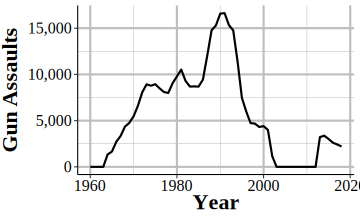
\includegraphics[width=1\linewidth,height=1\textheight]{index_files/figure-latex/nycGunAssaults-1} 

}

\caption{Monthly reports of gun assaults in New York City, 1960-2022.}\label{fig:nycGunAssaults}
\end{figure}

Given that agencies can join or drop out of the SRS program
at will, and report only partial data, it is highly
important to carefully examine your data to make sure that
there are no issues caused by this.

Even when an agency reports SRS data, and even when they
report every crime category, they can report fewer than 12
months of data. In some cases they simply report all of
their data in December, or report quarterly or semi-annually
so some months have zero crimes reported while others count
multiple months in that month's data. One example of this is
New York City, shown in Figure \ref{fig:nycMurderMonthly},
in the early-2000s to the mid-2010s where they began
reporting data quarterly instead of monthly.

\begin{figure}

{\centering 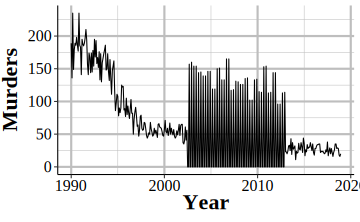
\includegraphics[width=1\linewidth,height=1\textheight]{index_files/figure-latex/nycMurderMonthly-1} 

}

\caption{Monthly murders in New York City, 1990-2022. During the 2000s, the police department began reporting quarterly instead of monthly and then resumed monthly reporting.}\label{fig:nycMurderMonthly}
\end{figure}

When you sum up each month into an annual count, as shown in
Figure \ref{fig:nycMurderYearly}, the problem disappears
since the zero months are accounted for in the months that
have the quarterly data. If you are using monthly data and
only examine the data at the annual level, you will fall
into the trap of having incorrect data that is hidden due to
the level of aggregation examined. While cases like NYC are
obvious when viewed monthly, for people that are including
thousands of agencies in their data, it is unfeasible to
look at each agency for each crime included. This can
introduce errors as the best way to examine the data is
manually viewing graphs and the automated method, looking
for outliers through some kind of comparison to expected
values, can be incorrect.

\begin{figure}

{\centering 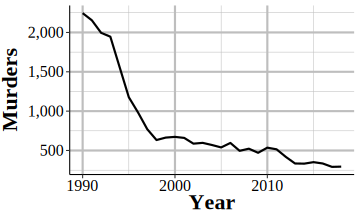
\includegraphics[width=1\linewidth,height=1\textheight]{index_files/figure-latex/nycMurderYearly-1} 

}

\caption{Annual murders in New York City, 1990-2022.}\label{fig:nycMurderYearly}
\end{figure}

In other cases when agencies report fewer than 12 months of
the year, they simply report partial data and as a result
undercount crimes. Figure \ref{fig:miamiDadeMurderAnnual}
shows annual murders in Miami-Dade, Florida and has three
years of this issue occurring. The first two years with this
issue are the two where zero murders are reported - this is
because the agency did not report any months of data. The
final year is in 2018, the last year of data in this graph,
where it looks like murder suddenly dropped significantly.
That is just because Miami-Dade only reported through June,
so they are missing half of 2018.

\begin{figure}

{\centering 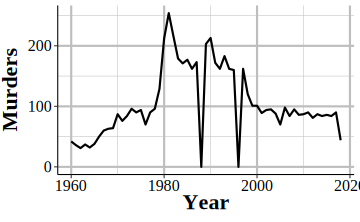
\includegraphics[width=1\linewidth,height=1\textheight]{index_files/figure-latex/miamiDadeMurderAnnual-1} 

}

\caption{Annual murders in Miami-Dade, Florida, 1960-2022.}\label{fig:miamiDadeMurderAnnual}
\end{figure}

\subsection{Zero crimes vs no
reports}\label{zero-crimes-vs-no-reports}

When an agency does not report, we see it in the data as
reporting zero crimes, not reporting NA or any indicator
that they did not report. In cases where the agency says
they did not report that month we can be fairly sure (not
entirely since that variable is not always accurate) that
the zero crimes reported are simply that the agency did not
report. In cases where the agency says they report that
month but report zero crimes, we cannot be sure if that is a
true no crimes reported to the agency or the agency not
reporting to the SRS. As agencies can report some crimes but
not others in a given month and still be considered
reporting that month, just saying they reported does not
mean that the zero is a true zero.

In some cases it is easy to see when a zero crimes reported
is actually the agency not reporting. As Figure
\ref{fig:nycGunAssaults} shows with New York City gun
assaults, there is a massive and sustained drop-off to zero
crimes and then a sudden return years later. Obviously,
going from hundreds of crimes to zero crimes is not a matter
of crimes not occurring anymore, it is a matter of the
agency not reporting - and New York City did report other
crimes these years so in the data it says that they reported
every month. So in agencies which tend to report many crimes
- and many here can be a few as 10 a year since going from
10 to 0 is a big drop - a sudden report of zero crimes is
probably just non-reporting.

Differentiating zero crimes and no reports becomes tricky in
agencies that tend to report few crimes, which most small
towns do. As an example, Figure \ref{fig:danvilleRape} shows
the annual reports of rape in Danville, California, a city
of approximately 45,000 people. The city reports on average
2.8 rapes per year and in five years reported zero rapes. In
cases like this it is not clear whether we should consider
those zero years as true zeros (that no one was raped or
reported their rape to the police) or whether the agency
simply did not report rape data that year.

\begin{figure}

{\centering 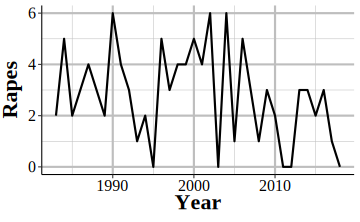
\includegraphics[width=1\linewidth,height=1\textheight]{index_files/figure-latex/danvilleRape-1} 

}

\caption{Annual rapes reported in Danville, CA, 1960-2022.}\label{fig:danvilleRape}
\end{figure}

\subsection{Agency data covered by another
agency}\label{agency-data-covered-by-another-agency}

\chapter*{About the Author}\label{about-the-author}


\textbf{Jacob Kaplan}

I am a Professional Specialist at the School of Public and
International Affairs (SPIA) and a member of Criminal
Justice @ SPIA at Princeton University. My research focuses
on law enforcement, including its impact on violent crime,
the influence of removing `bad apple' officers on reducing
complaints against officers, the extent to which police
forces represent the civilian populations they serve, and
the role of race and political affiliations in shaping
officer behavior. In addition to this, I conduct
methodological research focused on the quality and usability
of crime data, with a special emphasis on the FBI's Uniform
Crime Reporting (UCR) Program.

I am the author of
\emph{\href{https://www.routledge.com/A-Criminologists-Guide-to-R-Crime-by-the-Numbers/Kaplan/p/book/9781032244075}{A
Criminologist's Guide to R: Crime by the Numbers (Chapman \&
Hall/CRC The R Series, 2022)}}, an introductory textbook on
the R programming language tailored for crime research, with
a special focus on data cleaning and analysis. In addition,
I have developed several R packages, including
\href{https://jacobkap.github.io/fastDummies/}{fastDummies},
\href{https://jacobkap.github.io/asciiSetupReader/}{asciiSetupReader},
and
\href{https://jacobkap.github.io/predictrace/}{predictrace},
to streamline the data analysis process for researchers. My
website, \href{https://crimedatatool.com/}{Crime Data Tool},
offers users an interactive platform to explore crime data
from thousands of agencies across hundreds of variables
(e.g., arrests, offenses, demographics)---no data or
programming skills required.

My research has been published in leading academic journals,
such as the \emph{Journal of Quantitative Criminology},
\emph{Journal of Research in Crime and Delinquency},
\emph{Journal of Interpersonal Violence}, and \emph{American
Political Science Review}. I hold a B.S. in Criminal Justice
from California State University, Sacramento, and a M.S. and
Ph.D.~in Criminology from the University of Pennsylvania. I
previously served on the FBI's Criminal Justice Information
Services (CJIS) Advisory Policy Board (APB) Uniform Crime
Reporting (UCR) Subcommittee.

\mainmatter

\part{Summary Reporting System
(SRS)}\label{part-summary-reporting-system-srs}

\chapter{SRS Overview}\label{SRSGeneral}

One of the first, and most important, questions I think
people have about crime is a simple one: is crime going up?
Answering it seems simple - you just count up all the crimes
that happen in an area and see if that number of bigger than
it was in previous times.

However, putting this into practice invites a number of
questions, all of which affect how we measure crime. First,
we need to define what a crime is. Not philosophically what
actions are crimes - or what should be crimes - but
literally which of the many thousands of different criminal
acts (crimes as defined by state or federal law) should be
considered in this measure. Should murder count? Most people
would say yes. How about jaywalking or speeding? Many would
say probably not. Should marital rape be considered a crime?
Now, certainly most people (all, I would hope) would say
yes. But in much of the United States it was not a crime
until the 1970s
\citep{bennice2003marital, mcmahon2009criminalizing}. What
about marijuana possession, an act that is illegal
nationally and in some states, but legal elsewhere?

Next, we have to know what geographic and time unit to
measure crimes at since these decisions determine how
precise we can measure crime and when it changed. That is,
if you are mugged on Jan 1st at exactly 12:15pm right
outside your house, how do we record it? Should we be as
precise as including the exact time and location (such as
your home address)? Out of privacy concerns to the victim,
should we only include a larger time unit (such as hour of
the day or just the day without any time of day) or a larger
geographic unit (such as a Census Tract or the city)? And
what about when there are questions about geographic
jurisdiction such as a local police and sheriff overlapping
in their patrol area? Or when a crime happens over the
course of several hours (e.g.~a length burglary or
kidnapping)? Should we count the start time, the end time,
or somewhere in the middle?

The final question is that when a crime occurs, how do we
know? That is, when we want to count how many crimes
occurred do we ask people how often they've been victimized,
do we ask people how often they commit a crime, do we look
at crimes reported to police, crimes charged in a criminal
court? Each of these measures will likely give different
answers as to how many crimes
occurred.\footnote{The Bureau of Justice Statistics does measure crime by asking a random sample of people whether they were the victim of a crime. For more on this, please see their National Crime Victimization Survey reports}
And what about crimes where a victim reports it and the
police investigate and decide that it did not occur
(e.g.~victim reports an act which was not actually illegal)?
Or where the police say a crime occurred by the local
District Attorney declines to prosecute?

The FBI answered all of these questions in 1929 when they
began the Uniform Crime Reporting (SRS) Program Data, or SRS
data for short. \textbf{Crime consists of eight crime
categories - murder, rape, robbery, aggravated assault,
burglary, motor vehicle theft, theft, and simple assault -
that are reported to the police and is collected each month
from each agency in the country.} So essentially we know how
many of a small number of crime categories happen each month
in each city (though some cities have multiple police
agencies so even this is more complicated than it seems).
These decisions, born primarily out of the resource
limitations of 1929 (i.e.~no computers), have had a major
impact on criminology research. The first seven crime
categories - known as ``Index Crimes'' or ``Part 1 crimes''
(or ``Part I'' sometimes) - are the ones used to measure
crime in many criminology papers, even when the researchers
have access to data that covers a broader selection of
crimes than these.\footnote{Arson is also an index crime but
  was added after these initial seven were chosen and is not
  included in the crimes dataset (though is available
  separately) so is generally not included in studies that
  use index crimes.} These are also the crimes that the news
uses each year to report on how crime in the United States
compares to the previous year. The crime data actually also
includes the final crime, simple assault, though it is not
included as an index crime and is, therefore, generally
ignored by researchers - a large flaw in most studies that
we will discuss in more detail in Section \ref{indexCrimes}.
In fact excluding simple assault is such a large issue that
doing so has led us to exclude the most common violent crime
from most government, news, and academic reports, leading to
an undercount of violence in this country by approximately
50\%.

In this chapter we will provide a brief overview of the
datasets that make up the FBI's Summary Reporting System
(SRS) which you can think of as the ``aggregate'' data
collection that is part of their Uniform Crime Reporting
(UCR) Program Data. These datasets are primarily focused on
aggregate data, mostly having monthly counts of crimes
without many details about any particular crime. In
comparison, the other half of the UCR collection, the
National Incident-Based Reporting System (NIBRS) data is
focused entirely on providing detail on every individual
crime reported to the police. You can actually convert NIBRS
data to SRS in most cases - and FBI does for agencies that
report only NIBRS data - but there is no way to go from SRS
to NIBRS.

\section{Crimes included in the SRS
datasets}\label{crimes-included-in-the-srs-datasets}

SRS data covers only a subset - and for the crime data, a
very small subset - of all crimes that can occur. It also
only includes crimes reported to the police. So there are
two levels of abstraction from a crime occurring to it being
included in the data: a crime must occur that is one of the
crimes included in one of the SRS datasets (we detail all of
these crimes below) \emph{and} the victim must report the
incident to the police. While the crimes included are only a
small selection of crimes - which were originally chosen
since at the time the SRS was designed these were considered
important offenses and among the best reported - this is an
important first step to understanding the data.

SRS data should be understood as a loose collection of data
that seeks to understand crimes and arrests in the United
States. There are seven datasets in the SRS collection that
each cover a different topic or a subset of a previously
covered topic: crimes, arrests, property crimes
specifically, homicides specifically, police officers killed
or assaulted, arson specifically, and hate
crimes.\footnote{There is also a human trafficking dataset
  though this is a newer dataset and rarely used so I will
  not cover it in this book.} In this section we will go
over the crimes included in the two main SRS datasets:
Offenses Known and Clearances by Arrest and (which I like to
call the ``crime'' dataset) and the Arrests by Age, Sex, and
Race (the ``arrests'' dataset). These are the most commonly
used SRS datasets and the stolen property and homicide
datasets are simply more detailed subsets of these datasets.
The hate crime dataset can cover a broader selection of
offenses than in the crimes or arrests data, so we will
discuss those in Chapter @ref(hate\_crimes).

\section{A summary of each SRS
dataset}\label{a-summary-of-each-srs-dataset}

The SRS collection of data can be roughly summarized into
two groups: crime data and arrest data. While there are
several datasets included in the SRS data collection, they
are all extensions of one of the above groups. For arrest
data, you have information about who (by race and by
age-gender, but not by race-gender or race-age other than
within race you know if the arrestee is an adult or a
juvenile) was arrested for each crime. For crime data, you
have monthly counts of a small number of crimes (many fewer
than crimes covered in the arrest data) and then more
specialized data on a subset of these crimes - information
on homicides, hate crimes, assaults or killings of police
officers, and stolen property.

Each of these datasets will have its own chapter in this
book where we discuss the data thoroughly. Here is a very
brief summary of each dataset which will help you know which
one to use for your research. I still recommend reading that
data's chapter since it covers important caveats and uses
(or misuses) of the data that would not be covered below.

\subsection{Offenses Known and Clearances by Arrest (1960 -
present)}\label{offenses-known-and-clearances-by-arrest-1960---present}

The Offenses Known and Clearances by Arrest dataset - often
called Return A, ``Offenses Known'' or, less commonly, OKCA
- is the oldest and most commonly used dataset and measures
crimes reported to the police. For this reason it is used as
\emph{the} main measure of crime in the United States, and I
tend to call it the ``crimes dataset.'' This data answers
the most basic questions about crimes: how many occurred? If
you see crime data referenced in a news or academic article
it is usually this data. This data also includes the number
of crimes solved (though with a weaker definition of
``solved'' than you may think) and the number of crimes in
which the agency concluded did not actually occur which they
call an ``unfounded'' crime. This data has the monthly
number of crimes - for a select group of crimes types - that
occurred in an agency, as well as how many the police
investigated and decided did not occur, and the number
``cleared'' by an arrest. The data uses something called a
Hierarchy Rule which means that in incidents with multiple
crimes, only the most serious is recorded - though in
practice this affects only a small percent of cases, and
primarily affects property crimes.

\subsection{Arrests by Age, Sex, and Race (1974 -
present)}\label{arrests-by-age-sex-and-race-1974---present}

The Arrests by Age, Sex, and Race dataset - often called
ASR, or the ``arrests data'', or sometimes the ``Arrests by
Age, Sex, Race, and Ethnicity though this is really
misleading since most years do not even report ethnicity
data - includes the monthly number of arrests for a variety
of crimes and, unlike the crime data, breaks down this data
by age and gender. This data includes a broader number of
crime categories than the crime dataset (the Offenses Known
and Clearances by Arrest data) though is less detailed on
violent crimes since it does not breakdown aggravated
assault or robberies by weapon type as the Offenses Known
data does.

For each crime it says the number of arrests for each
gender-age group with younger ages (15-24) showing the
arrestee's age to the year (e.g.~age 16, age 17) and other
ages grouping years together (e.g.~age 25-29, 30-34, ``under
10''). It also breaks down arrests by race-age by including
the number of arrestees of each race (American Indian,
Asian, Black, and White are the only included races) and if
the arrestee is a juvenile (\textless18 years old) or an
adult. The data does technically include a breakdown by
ethnicity-age (e.g.~juvenile-Hispanic,
juvenile-non-Hispanic) but almost no agencies report this
data (for most years zero agencies report ethnicity at all)
so in practice the data does not include ethnicity. As the
data includes counts of arrestees, people who are arrested
multiple times are included in the data multiple times - it
is not a measure of unique arrestees.

\subsection{Law Enforcement Officers Killed and Assaulted
(LEOKA) (1960 -
present)}\label{law-enforcement-officers-killed-and-assaulted-leoka-1960---present}

The Law Enforcement Officers Killed and Assaulted data,
often called just by its acronym LEOKA (``LEE-OH-KUH''), has
two main purposes.\footnote{This data is also sometimes
  called the ``Police Employees'' dataset.} First, it
provides counts of employees employed by each agency -
broken down by if they are civilian employees or sworn
officers, and also broken down by sex (male and female are
the only options). And second, it measures how many officers
were assaulted or killed (including officers who die
accidentally such as in a car crash) in a given month. The
assault data is also broken down into shift type
(e.g.~alone, with a partner, on foot, in a car, etc.), the
offender's weapon, and type of call they are responding to
(e.g.~robbery, disturbance, traffic stop). The killed data
simply says how many officers are killed feloniously
(i.e.~murdered) or died accidentally (e.g.~car crash) in a
given month. The employee information is at the year-level
so you know, for example, how many male police officers were
employed in a given year at an agency, but do not know any
more than that such as if the number employed changed over
the year. This dataset is commonly used as a measure of
police employees and is a generally reliable measure of how
many police are employed by a police agency. The second part
of this data, measuring assaults and deaths, is more flawed
with missing data issues and data error issues (e.g.~more
officers killed than employed in an agency).

\subsection{Supplementary Homicide Reports
(SHR)}\label{supplementary-homicide-reports-shr}

The Supplementary Homicide Reports dataset - often
abbreviated to SHR - is the most detailed of the SRS
datasets and provides information about the circumstances
and participants (victim and offender demographics and
relationship status) for homicides. For each homicide
incident it tells you the age, gender, race, and ethnicity
of each victim and offender as well as the relationship
between the first victim and each of the offenders (but not
the other victims in cases where there are multiple
victims). It also tells you the weapon used by each offender
and the circumstance of the killing, such as a ``lovers
triangle'' or a gang-related murder. As with other SRS data,
it also tells you the agency it occurred in and the month
and year when the crime happened.

One important point of clarification: this is not the number
of murders, though it does track that. This data also
includes the number of homicides that are manslaughter by
negligence (e.g.~children playing with a gun, hunting
accident) and justifiable homicides (i.e.~not criminal). So
be carefully when speaking about this data. It is murders
but not only murders so you want to speak precisely.

\subsection{Hate Crime Data (1991 -
present)}\label{hate-crime-data-1991---present}

This dataset covers crimes that are reported to the police
and judged by the police to be motivated by hate. More
specifically, they are (1) crimes which were (2) motivated -
at least in part - by bias towards a certain person or group
of people because of characteristics about them such as
race, sexual orientation, or religion. The first part is
key, they must be crimes - and really must be the selection
of crimes that the FBI collects for this dataset. Biased
actions that do not meet the standard of a crime, or are of
a crime category not included in this data, are not
considered hate crimes. For example, if someone yells at a
Black person and uses racial slurs against them, it is
clearly a racist action. For it to be included in this data,
however, it would have to extend to a threat since
``intimidation'' is a crime included in this data but lesser
actions such as simply insulting someone is not included.
For the second part, the bias motivation, it must be against
a group that the FBI includes in this data. For example,
when this data collection began in 1991 crimes against
transgender people were not counted so if a transgender
person was assaulted or killed because they were
transgender, this is not a hate crime recorded in the data
(though it would have counted in the ``Anti-Lesbian, Gay,
Bisexual, Or Transgender, Mixed Group (LGBT)'' bias
motivation which was always reported).

\subsection{Property Stolen and Recovered (Supplement to
Return A) (1960 -
present)}\label{property-stolen-and-recovered-supplement-to-return-a-1960---present}

The Property Stolen and Recovered data - sometimes called
the Supplement to Return A (Return A being another name for
the Offenses Known and Clearances by Arrest dataset, the
``crime'' dataset) - provides monthly information about
property-related offenses (theft, motor vehicle theft,
robbery, and burglary), including the location of the
offense (in broad categories like ``gas station'' or
``residence''), what was stolen (e.g.~clothing, livestock,
firearms), and how much the stolen items were
worth.\footnote{It also includes the value of items stolen
  during rapes and murders, if anything was stolen.} It also
includes robberies so is really the ``stuff taken during a
crime'' dataset than the dataset about property crimes. The
``recovered'' part of this dataset covers the type and value
of property recovered so you can use this, along with the
type and value of property stolen, to determine what percent
and type of items the police managed to recover.

Like most other SRS datasets this is at the agency-month
level so you can, for example, learn how often burglaries
occur at the victim's home during the day, and if that rate
changes over the year or differs across agencies. The data,
however, provides no information about the offender or the
victim (other than if the victim was an individual or a
commercial business \footnote{based on the location of the
  incident - ``bank'', ``gas station'', etc.}). The value of
the property stolen is primarily based on the victim's
estimate of how much the item is worth (items that are
decreased in value once used - such as cars - are supposed
to be valued at the current market rate, but the data
provides no indication of when it uses the current market
rate or the victim's estimate) so it should be used as a
very rough estimate of value.

\subsection{Arson (1979 -
present)}\label{arson-1979---present}

The arson dataset provides monthly counts at the police
agency-level for arsons that occur, and includes a breakdown
of arsons by the type of arson (e.g.~arson of a person's
home, arson of a vehicle, arson of a community/public
building) and the estimated value of the damage caused by
the arson. This data includes all arsons reported to the
police or otherwise known to the police (e.g.~discovered
while on patrol) and also has a count of arsons that lead to
an arrest (of at least one person who committed the arson)
and reports that turned out to not be arsons (such as if an
investigation found that the fire was started accidentally).
This is essentially the Offenses Known and Clearances by
Arrest data but only for arsons. The data even follows the
same definitions for categories such as what counts as a
cleared or unfounded crime. The primary additional variable
is the estimated damage in dollars caused by the arson.

\chapter{Offenses Known and Clearances by
Arrest}\label{offensesKnown}

The Offenses Known and Clearances by Arrest dataset - often
called Return A, ``Offenses Known'' or, less commonly, OKCA
- is the oldest and most commonly used dataset in the UCR
and measures it crimes reported to the police. For this
reason it is used as \emph{the} main measure of crime in the
United States, and I tend to call it the ``crimes dataset.''
This data answers the most basic questions about crimes: how
many occurred? If you see crime data referenced in a news or
academic article it is usually this data. This data also
includes the number of crimes solved (though with a weaker
definition of ``solved'' than you may think) and the number
of crimes in which the agency concluded did not actually
occur which they call an ``unfounded'' crime. This data has
the monthly number of crimes - for a select group of crimes
types - that occurred in an agency, as well as how many the
police investigated and decided did not occur, and the
number ``cleared'' by an arrest.

The Offenses Known data has been \textbf{the} crime data of
record for nearly a century, and will likely still be for
the next couple of decades at least. And that is due to its
simplicity. This data is (with some exceptions we will get
into) just the monthly number of crimes reported or
otherwise known (e.g.~discovered while on patrol) to a
police agency for a small number of crimes. If you want to
know, for example, how many murders or burglaries happened
in your city last year, this is the dataset to turn to. This
simplicity allows a much wider group of people to use the
data; since it is monthly counts of crimes (with no
breakdown by location, race, age, injury, etc.) you do not
need much programming or analytic skills to use it.

I argued earlier in this book that NIBRS is a far superior
dataset than anything in SRS, and I stand by that. NIBRS is
superior in nearly every way. But for most people - the
general public, reporters, many academics, etc. - what is
important is ease of use and very basic descriptive
statistics such as how many crimes happened in my city last
year\footnote{Even some academic papers are little more than
  a difference between two or more cities over time and can
  be very good research even if the data is not that
  complex.}, and is it getting more dangerous than it used
to be? The Offenses Known data answers that, at least to a
point. You can answer more complex questions using NIBRS but
most people do not need those questions answered. They're
content with what can be answered using the Offenses Known
data. And for good reason. ``Is crime increasing in my
city'' is really the first and most important question about
crime that people have.

Part of the superiority of NIBRS is that while it can answer
much more complex questions than SRS datasets, it can also
answer the same questions that the SRS can. That is because,
by design, NIBRS collects the same information as SRS and
can be converted to SRS data. Many agencies that submit
NIBRS data do not submit SRS data at all, and the FBI
converts the NIBRS data to its SRS counterpart for release
to the public. This is an almost perfect comparison but not
all of the same variables are collected, which will cause
some issues that we will discuss in this chapter.

One thing you may have heard about this data is that it uses
something called the Hierarchy Rule. Basically the rule says
that when an incident involves more than one crime, such as
a robbery and a murder, you only count the most serious
crime. And most serious is based on the hierarchy the FBI
has created. This is true and therefore the number of crimes
- other than murder which is the most serious - recorded in
this data is always an undercount. But you really should not
be too concerned about this. As we will get into below, the
Hierarchy Rule affects only a relatively small share of
incidents so does not undercount crime by too much - and
when it does it is primarily undercounting property crime.

\section{Which crimes are
included?}\label{indexCrimesOffensesKnown}

This dataset contains information on the number of ``Index
Crimes'' (sometimes called Part I crimes) reported to each
agency.\footnote{While some people capitalize ``Index
  Crime,'' I prefer the term in lowercase which is how I
  will write it.} These index crimes are a collection of
eight crimes that, for historical reasons based largely by
perceived importance and reliability of their reporting in
the 1920s when the UCR program was first developed, are used
as the primary measure of crime today. Other data sets in
the UCR, such as the Arrests by Age, Sex, and Race data and
the Hate Crime data have more crimes reported.

The crimes are, in order by the Hierarchy Rule (which we
will discuss next):

\begin{enumerate}
\def\labelenumi{\arabic{enumi}.}
\tightlist
\item
  Homicide\\
\end{enumerate}

\begin{itemize}
\tightlist
\item
  Murder and non-negligent manslaughter\\
\item
  Manslaughter by negligence
\end{itemize}

\begin{enumerate}
\def\labelenumi{\arabic{enumi}.}
\setcounter{enumi}{1}
\tightlist
\item
  Rape\\
\end{enumerate}

\begin{itemize}
\tightlist
\item
  Rape\\
\item
  Attempted rape\\
\end{itemize}

\begin{enumerate}
\def\labelenumi{\arabic{enumi}.}
\setcounter{enumi}{2}
\tightlist
\item
  Robbery\\
\end{enumerate}

\begin{itemize}
\tightlist
\item
  With a firearm\\
\item
  With a knife of cutting instrument\\
\item
  With a dangerous weapon not otherwise specified\\
\item
  Unarmed - using hands, fists, feet, etc.\\
\end{itemize}

\begin{enumerate}
\def\labelenumi{\arabic{enumi}.}
\setcounter{enumi}{3}
\tightlist
\item
  Aggravated Assault (assault with a weapon or with the
  intent to cause serious bodily injury)\\
\end{enumerate}

\begin{itemize}
\tightlist
\item
  With a firearm\\
\item
  With a knife of cutting instrument\\
\item
  With a dangerous weapon not otherwise specified\\
\item
  Unarmed - using hands, fists, feet, etc.\\
\end{itemize}

\begin{enumerate}
\def\labelenumi{\arabic{enumi}.}
\setcounter{enumi}{4}
\tightlist
\item
  Burglary\\
\end{enumerate}

\begin{itemize}
\tightlist
\item
  With forcible entry\\
\item
  Without forcible entry\\
\item
  Attempted burglary with forcible entry\\
\end{itemize}

\begin{enumerate}
\def\labelenumi{\arabic{enumi}.}
\setcounter{enumi}{5}
\tightlist
\item
  Theft (other than of a motor vehicle)\\
\item
  Motor Vehicle Theft\\
\end{enumerate}

\begin{itemize}
\tightlist
\item
  Cars\\
\item
  Trucks and buses\\
\item
  Other vehicles\\
\end{itemize}

\begin{enumerate}
\def\labelenumi{\arabic{enumi}.}
\setcounter{enumi}{7}
\tightlist
\item
  Arson\\
\item
  Simple Assault
\end{enumerate}

Arson is considered an index crime but is not reported in
this data - you need to use the separate Arson dataset of
the UCR to get access to arson counts. See Chapter
\ref{arsonChapter} for an overview of the Arson data. The
ninth crime on that list, simple assault, is not considered
an index crime but is nevertheless included in this data.

Each of the crimes in the list above, and their
subcategories, are included in the UCR data. In most news
and academic articles, however, you will see them reported
as the total number of index crimes, summing up categories
1-7 and reporting that as ``crime.''\footnote{I have
  encountered a shocking number of academic papers and
  researchers who seem to believe that the subcategories are
  not included in the data at all.} These index crimes are
often divided into violent index crimes - murder, rape,
robbery, and aggravated assault - and property index crimes
- burglary, theft, motor vehicle theft. For more on index
crimes, and the drawbacks of using them, please see Section
\ref{indexCrimes}.

\subsection{Hierarchy Rule}\label{hierarchy}

This dataset uses what is called the Hierarchy Rule where
only the most serious crime in an incident is reported
(except for motor vehicle theft and arson, which are always
included).\footnote{FBI documentation actually differs on
  whether motor vehicle theft is always reported with some
  documentation saying it is while others placing it in the
  hierarchy. According to their ``Summary Reporting System
  (SRS) User Manual'' Version 1.0 released 6/20/2013, ``The
  offenses of justifiable homicide, motor vehicle theft, and
  arson are exceptions to the Hierarchy Rule.''} For example
if there is an incident where the victim is robbed and then
murdered, only the murder is counted as it is considered
more serious than the robbery. That the data uses the
Hierarchy Rule is a frequently cited (by academics,
reporters, random people on Twitter) criticism of the data
that is, in my opinion, overblown.

In practice, the Hierarchy Rule has only modest effects on
the data, undercounting few crimes. Though the Hierarchy
Rule does mean this data is an undercount, data from other
sources indicate that it is not much of an under count.
NIBRS data contains every crime that occurs in an incident
(i.e.~it does not use the Hierarchy Rule). Using this we can
measure how many crimes the Hierarchy Rule excludes. In
approximately 90\% of incidents, only one crime is
committed.\footnote{According to 2022 NIBRS, 88.15\% of
  incidents have only a single offense.} Additionally, when
people talk about ``crime'' they usually mean murder which,
while incomplete to discuss crime, means the UCR data here
is accurate on that measure.

The FBI released a report
\href{https://ucr.fbi.gov/nibrs/2014/resource-pages/effects_of_nibrs_on_crime_statistics_final.pdf}{available
here} in 2015 that directly examined this issue by taking
NIBRS data from 2014 and examined how NIBRS data (which does
not use the Hierarchy Rule) compares to using the Hierarchy
Rule and keeping only the most serious crime. Figure
\ref{fig:fbiHierarchy} is a screenshot from their report
showing the percent increases in crimes when including all
crimes in an incident relative to following the Hierarchy
Rule. They find that 10.6\% of incidents have multiple
crimes occurring. For violent crime, murder and rape have no
change; for the remaining violent crimes - robbery and
aggravated assault - crimes increased by 0.6\%.\footnote{Murder
  is not shown in this figure since murder is always
  reported so cannot change.} Burglary increased by 1\% and
the largest increases came from theft and motor vehicle
theft, increasing by 2.6\% and 2.7\%, respectively.
Curiously, motor vehicle theft increased even though the
FBI's documentation for this data says that it is exempt
from the Hierarchy Rule and should always be reported. This
discrepancy suggests either non-compliance or errors in the
FBI's manual.

\begin{figure}

{\centering \includegraphics[width=1\linewidth,height=1\textheight]{images/fbi_hierarchy} 

}

\caption{The FBI's findings of how crime reporting changes when using the Hierarchy Rule using NIBRS 2014 data.}\label{fig:fbiHierarchy}
\end{figure}

In Table \ref{tab:nibrsHierarchy} I replicate the FBI's
table using NIBRS 2022 data. Results are fairly close.
Homicide and rape and unchanged; robbery and aggravated
assault both increase by \textless1\%; my count for theft
and burglary are a bit smaller, and motor vehicle theft is
almost triple the FBI's 2014 number. But these numbers are
mostly consistent - particularly so for violent crime - and
I expect the differences are just that 2014 and 2022 data
are different. So using the Hierarchy Rule does undercount
crime, but this is a small undercounting and is primarily
led by property crime. Violent crime is only slightly
undercounted. And compared to the number of crimes not
counted because the victim does not reports it to the
police, this is a very small share of crimes.

\begin{longtable}[t]{ll}
\caption{\label{tab:nibrsHierarchy}The percent increase in reported crimes for each index crime if the Hierarchy Rule was not used, NIBRS 2022.}\\
\toprule
Crime & \% increase without Hierarchy Rule\\
\midrule
\endfirsthead
\caption[]{\label{tab:nibrsHierarchy}The percent increase in reported crimes for each index crime if the Hierarchy Rule was not used, NIBRS 2022. \textit{(continued)}}\\
\toprule
Crime & \% increase without Hierarchy Rule\\
\midrule
\endhead

\endfoot
\bottomrule
\endlastfoot
Homicide & 0.00\\
Rape & 0.03\\
Robbery & 0.54\\
Aggravated Assault & 0.82\\
Burglary & 1.57\\
\addlinespace
Theft & 1.47\\
Motor Vehicle Theft & 7.92\\
Arson & 7.54\\*
\end{longtable}

\subsection{Index (``Part 1'') crimes}\label{indexCrimes}

One of the first things that people tend to learn about SRS
crime data is that it covers something called an ``index
crime.''\footnote{Index crimes are sometimes capitalized as
  ``Index Crimes'' though I have seen it written both ways.
  In this book I keep it lowercase as ``index crimes.''}
Index crimes, sometimes written as Part 1 or Part I crimes,
are the seven crimes originally chosen by the FBI to be
included in their measure of crimes as these offenses were
both considered serious and generally well-reported so would
be a useful measure of crime. Index crimes are often broken
down into property index crimes - burglary, theft, and motor
vehicle theft (and arson now, though that is often not
included and is reported less often by agencies) - and
violent index crimes (murder, rape, robbery, and aggravated
assault). The ``index'' is simply that all of the crimes are
summed up into a total count of crimes (violent, property,
or total) for that police agency.

The biggest problem with index crimes is that it is simply
the sum of 8 (or 7 since arson data usually isn't included)
crimes. Index crimes have a huge range in their seriousness
- it includes, for example, both murder and theft - so
summing up the crimes gives each crime equal weight. This
approach is flawed as 100 murders is more serious than 100
thefts. This is especially a problem as less serious crimes
(theft mostly) are far more common than more serious crimes.
In 2017, for example, there were 1.25 million violent index
crimes in the United States. That same year had 5.5 million
thefts. So using index crimes as your measure of crimes
fails to account for the seriousness of crimes. Looking at
total index crimes is, in effect, mostly just looking at
theft. Looking at violent index crimes alone mostly measures
aggravated assault. This is especially a problem because it
hides trends in violent crimes. As an example, San
Francisco, shown in Figure \ref{fig:sfThefts}, has had a
huge increase - about 50\% - in index crimes in the last
several years. When looking closer, that increase is driven
almost entirely by the near doubling of theft since 2011.
During the same years, index violent crimes have stayed
fairly steady. So the city isn't getting more dangerous - at
least not in terms of violent index crimes increasing - but
it appears like it is due to just looking at total index
crimes.

\begin{figure}

{\centering 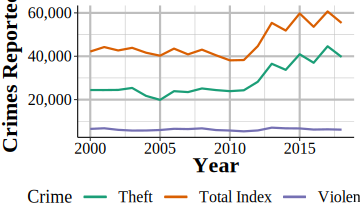
\includegraphics[width=1\linewidth,height=1\textheight]{03_offenses_known_files/figure-latex/sfThefts-1} 

}

\caption{Thefts and total index crimes in San Francisco, 2000-2022.}\label{fig:sfThefts}
\end{figure}

Many researchers divide index crimes into violent and
nonviolent categories, which helps but even this is not
entirely sufficient. Take Chicago as an example. It is a
city infamous for its large number of murders. But as a
fraction of index crimes, Chicago has a rounding error worth
of murders. Their 653 murders in 2017 is only 0.5\% of total
index crimes. For violent index crimes, murder made up 2.2\%
of crimes that year. As seen in Figure
\ref{fig:chicagoMurder}, in no year where data is available
did murders account for more than 3.5\% of violent index
crimes; and, while murders are increasing as a percent of
violent index crimes they still account for no more than
2.5\% in most recent years. What this means is that changes
in murder are very difficult to detect. If Chicago had no
murders this year, but a less serious crime (such as theft)
increased slightly, we could not tell from looking at the
number of index crimes, even from violent index crimes. As
discussed in the below section, using this sample of crimes
as the primary measure of crimes - and particularly of
violent crimes - is also misleading as it excludes important
- and highly common relative to index crimes - offenses,
such as simple assault.

\begin{figure}

{\centering 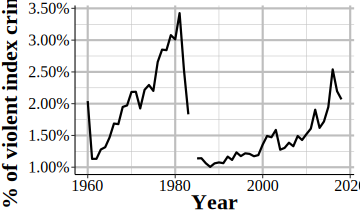
\includegraphics[width=1\linewidth,height=1\textheight]{03_offenses_known_files/figure-latex/chicagoMurder-1} 

}

\caption{Murders in Chicago as a percent of violent index crimes, 1960-2022.}\label{fig:chicagoMurder}
\end{figure}

\subsubsection{What is a violent
crime?}\label{what-is-a-violent-crime}

An important consideration in using this data is defining
what a ``violent crime'' is. One definition, and the one
that I think makes the most sense, is that a violent crime
is one that uses force or the threat of force. For example,
if I punch you in the face, that is a violent crime. If I
stab you, that is a violent crime. While clearly different
in terms of severity, both incidents used force so I believe
would be classified as a violent crime. The FBI, and most
researchers, reporters, and advocates would disagree.
Organizations ranging from the
\href{https://SRS.fbi.gov/crime-in-the-u.s/2019/crime-in-the-u.s.-2019/topic-pages/violent-crime}{FBI
itself} to
\href{https://www.pewresearch.org/fact-tank/2020/11/20/facts-about-crime-in-the-u-s/}{Pew
Research Center} and advocacy groups like the
\href{https://arresttrends.vera.org/data-sources-methodology}{Vera
Institute of Justice} and the
\href{https://www.aclu.org/report/tale-two-countries-racially-targeted-arrests-era-marijuana-reform}{ACLU}
all define the first example as a non-violent crime and the
second as a violent crime. They do this for three main
reasons.

The first reason is that simple assault is not an index
crime, so they do not include it when measuring violent
crime. It is almost a tautology in criminology that you use
index crimes as the measure of crime since that is just what
people do. As far as I am aware, this is really the main
reason why researchers justify using index crimes: because
people in the past used it so that is just what is done
now.\footnote{I have also seen the justification that
  aggravated assault is more serious since it uses a weapon,
  though as the SRS subcategory of aggravated assault
  without a weapon clearly shows, aggravated assault does
  not require use of a weapon.} This strikes me as a
particularly awful way of doing anything, more so since
simple assault data has been available almost as long as
index crime data.\footnote{Simple assault is first available
  in 1964. Index crime data is available since 1960.}

The second reason - and one that I think makes sense for
reporters and advocates who are less familiar with the data,
but should be unacceptable to researchers - is that people
do not know that simple assault is included, or at least do
not have easy access to it. Neither the FBI's annual report
\href{https://SRS.fbi.gov/crime-in-the-u.s/2019/crime-in-the-u.s.-2019/home}{page}
not their official
\href{https://crime-data-explorer.fr.cloud.gov/}{crime data
tool website} include simple assault since they only include
index crimes. For people who rely only on these sources -
and given that using the data itself requires at least some
programming skills, I think this accounts for most users and
certainly nearly all non-researchers - it is not possible to
access simple assault crime data (arrest data does include
simple assault on these sites) from these official sources.

The final reason is that it benefits some people's goals to
classify violent crime as only including index crimes. This
is because simple assault is extremely common compared to
violent index crimes - in many cities simple assault is more
common than all violent index crimes put together - so
excluding simple assault makes it seem like fewer arrests
are violent than they are when including simple assault. For
example, a number of articles have noted that marijuana
arrests are more common than violent crime arrests
\citep{ingraham2016, kertscher2019, devito2020, earlenbaugh2020, aclu2020}
or that violent crime arrests are only 5\% of all arrests
\citep{neusteter2019every, speri2019}.\footnote{The FBI's
  report for arrests does include simple assault so the
  second reason people may not include it does not apply
  here.} While true when considering only violent index
crimes, including simple assault as a violent crime makes
these statements false. Some organizations call the violent
index crimes ``serious violent crimes'' which is an
improvement but even this is a misnomer since simple assault
can lead to more serious harm than aggravated assault. An
assault becomes aggravated if using a weapon or there is the
\emph{potential} for serious harm, even if no harm actually
occurs.\footnote{SRS data provides no information about the
  harm caused to victims. The new FBI dataset NIBRS actually
  does have a variable that includes harm to the victim so
  if you are interested in measuring harm (an understudied
  topic in criminology), that is the dataset to use.}

As an example of this last point, Figure
\ref{fig:simpleIndex} shows the number of violent index
crimes and simple assaults each year from 1960 to 2018 in
Houston, Texas (simple assault is not reported in SRS until
1964, which is why 1960-1963 show zero simple assaults). In
every year where simple assault is reported, there are more
simple assaults than aggravated assaults. Beginning in the
late 1980s, there are also more simple assaults than total
violent index crimes. Excluding simple assault from being a
violent crime greatly underestimates violence in the
country.

\begin{figure}

{\centering 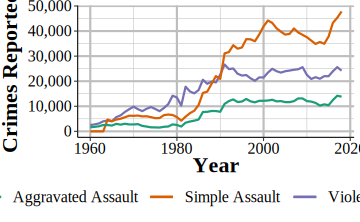
\includegraphics[width=1\linewidth,height=1\textheight]{03_offenses_known_files/figure-latex/simpleIndex-1} 

}

\caption{Reported crimes in Houston, Texas, from 1960 to 2018. Violent index crimes are aggravated assault, rape, robbery, and murder.}\label{fig:simpleIndex}
\end{figure}

\section{Agencies reporting}\label{offensesKnownReporting}

Figure \ref{fig:offensesAgenciesReporting} shows the annual
number of police agencies that reported at least one month
that year. With data starting in 1960, there were a little
under 7,500 agencies reporting a year until 1970 when the
number of agencies began increasing. This continued until
the late 1970s when about 14,000 agencies reported, and this
remained steady for over a decade before declining in the
1990s until about 12,500 in the latter half of the decade.
Then the number of agencies reporting increased steadily
until about 16,500 agencies reported in 2010. The number of
agencies has slowly increased since then, adding a few
hundred agencies from 2010 to 2020. The drop and then
partial recovery you see in 2021 and 2022 is from the FBI
stopping collection of this data and then restarting that
collection in 2021. Most agencies report to NIBRS but the
only that still report SRS, and therefore could not report
in 2021, caused the drop.

There are actually two lines throughout this entire figure,
though they are nearly identical until 2018. That is because
there are two ways of measuring how many months an agency
reports data. The primary one - and the one the FBI itself
uses - is through a variable in the data called the
``last\_month\_reported.'' This is, as it sounds, the last
month the agency sent data in. So if an agency reports data
in December the variable will have ``December'' as the last
month. If that agency only reported it December the variable
will still say ``December.'' Most people use this as the
number of months that the agency reported. So a December
value is 12 months reported, even though in our example it
was the only month with data.

In the data there are 12 columns - one for each month - that
says whether the agency reported data in that month. That is
what I use in the green line to measure how many months of
data that agency reported. I refer to this in the figure and
in the data I have released as the ``number of months
missing.'' When looking at agencies reporting only a single
month the lines are nearly identical, though the last month
reported measure is nearly always larger. This changes in
2018 as a result of the data changing, meaning I needed to
use different columns to check starting in that year. That
means that post-2018 data may not be comparable to 2018 and
earlier using this variable.

\begin{figure}

{\centering 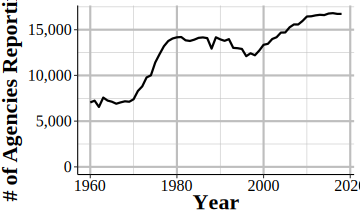
\includegraphics[width=1\linewidth,height=1\textheight]{03_offenses_known_files/figure-latex/offensesAgenciesReporting-1} 

}

\caption{The annual number of agencies reporting at least one month of data and a full 12 months of data, 1960-2022.}\label{fig:offensesAgenciesReporting}
\end{figure}

Usually when you are looking at crime data you want annual
data, so having agencies report a full year's of data is
more important than them submitting just partial data. This
is especially important when comparing an agency over time
or two different agencies to each other. Obviously, an
agency with 6 month of data will have fewer crimes reported
than one with 12 months reported, all else being equal. But
this is something easy to overlook as it is an easy
assumption that agencies will report a full years-worth of
data. Unfortunately, this is always true. Some agencies do
not report any data and others report only part of the year
- though if an agency reports one month they usually do
report all 12. Figure
\ref{fig:offensesAgenciesReportingFull} repeats Figure
\ref{fig:offensesAgenciesReporting} but now showing only
agencies reporting 12 months of data, using both of our
measures. Since 1960 every year has had fewer agencies
reporting full data using the ``number of months missing''
method than the ``last month reported'' method.

\section{Negative numbers}\label{negative-numbers}

One of the most common questions people have about this data
is why there are negative numbers, and if they are a
mistake. Negative numbers are not a mistake. The SRS data is
monthly so police agencies report the number of monthly
crimes that are known to them - either reported to them or
discovered by the police. In some cases the police will
determine that a crime reported to them did not actually
occur - which they called an ``unfounded crime.'' An example
that the FBI gives for this is a person reports their wallet
stolen (a theft) and then later finds it, so a crime was
initially reported but no crime actually occurred.

How this works when the police input the data is that an
unfounded crime is reported both as an unfounded crime and
as a negative actual crime - the negative is used to zero
out the erroneous report of the actual crime. So the report
would look like 1 actual theft (the crime being reported),
-1 theft (the crime being discovered as not have happened),
and 1 unfounded theft. If both incidents occurred in the
same month then this would simply be a single unfounded
theft occurring, with no actual theft - literally a value of
1 + -1 = 0 thefts.

Negative values occur when the unfounding happens in a later
month than the crime report. In the theft case, let us say
the theft occurred in January and the discovery of the
wallet happens in August. Assuming no other crimes occurred,
January would have 1 theft, and August would have -1 thefts
and 1 unfounded theft. There is no way of determining in
which month (or even which year) an unfounded crime was
initially reported in. When averaging over the long term,
there should not be any negative numbers as the actual and
unfounded reports will cancel themselves out. However, when
looking at monthly crimes - particularly for rare crimes -
you will still see negative numbers for this reason. Since
crimes can be unfounded for reports in previous years, you
can actually see entire year's crime counts be negative,
though this is much rarer than monthly values.\footnote{From
  1960-2022, there were 39 agency-years with a negative
  count of murders.}

So using the far more common last month reported method will
overestimate how many agencies report a full year of data.
In practice, though, this affects very little data and what
it does affect is only overcounted very slightly. At least
when aggregating nationally - which I generally advise
against since local crime matters a lot more than national
averages. Still, let us look the increase in the total
number of crimes reported by 12-month reporting agencies
increases from the ``number of months missing'' measure to
the ``last month reported'' measure, shown in Figure
\ref{fig:murdersBothMeasures}. The answer is an extremely
small increase, averaging (mean = 0.93\%, mean = 1.26\%)
about a one percent point increase each year. The
differences in measuring how many months are reported can
matter a great deal at the agency-level, but does very
little when aggregating nationally.

\begin{figure}

{\centering \includegraphics[width=1\linewidth,height=1\textheight]{03_offenses_known_files/figure-latex/murdersBothMeasures-1} 

}

\caption{The percent change in the number of murders reported in the United States each year when moving from the number of months missing measure to the last month reported measure, 1960-2020.}\label{fig:murdersBothMeasures}
\end{figure}

\section{Important variables}\label{important-variables}

Now let us talk about some important variables in this data
such as what it actually measures. For each crime we have
four different categories indicating the number of crimes
actually committed, the number cleared, and the number
determined to not have occurred. Like other UCR data, there
are also variables that provide information about the agency
- ORI codes, population under jurisdiction - the month and
year that the data covers, and how many months reported
data.

\subsection{Actual crimes}\label{actual}

This is the number of offenses that \emph{actually} occurred
- where \emph{actually} means that a police investigation
found that the crime report was accurate. Occurred is
actually a bit of a strong word. These are crimes that come
to the police's attention in that month, even if the crime
actually occurred before. For example, if someone walks into
a police department on February, 2025 and says ``last year I
killed five people'' that would count as five murders in
February, 2025 (that is assuming that the police believe
that the person is telling the truth). It would not be
counted in 2024 when the person says the murders took place.

Crimes that are reported that the police find did not occur
(e.g.~report of an arson but turns that the fire began
accidentally) are called ``unfounded'' crimes. So this
variable is the one people use to measure \emph{crime}. For
example if 10 people are murdered in a city the number of
``actual murders'' would be 10. A crime is a crime incident,
regardless of how many offenders there were. If there are
multiple victims in a case, such as a double murder, then it
would count as multiple crimes.

Figure \ref{fig:newarkMurders}, for example, shows the
number of murders per 100,000 population in Newark, NJ, for
1960-2022. One things stands out. Or does not stand out, in
a bad way. Newark Police did not report a full year of data
in 2015; they reported only 11 months. It is imperceptible
in the figure but if you look at the number of months
reported in that year - using either the last month reported
or the number of months missing measure - you can see that
December is missing. While visualizing the data is often a
good way to look for outliers or missingness, it is not
enough alone. You need to look at the raw data as well to be
safe.

\begin{figure}

{\centering \includegraphics[width=1\linewidth,height=1\textheight]{03_offenses_known_files/figure-latex/newarkMurders-1} 

}

\caption{The annual murder rate per 100,000 people in Newark, NJ, 1960-2022.}\label{fig:newarkMurders}
\end{figure}

Since this is the number of crimes reported and found to
occurred, it undercounts the total number of reported
crimes. To get that number you will need to add actual
crimes to unfounded crimes, which we discuss in Section
@ref(\{unfounded\}). However, unfounded crimes are
increasingly not being reported as agencies move to NIBRS
reporting which does not capture unfounded crimes.

\subsection{Total cleared crimes}\label{clearedCrimes}

A crime is cleared when an offender is arrested or when the
case is considered cleared by exceptional means. To be more
specific, this data counts crime as a crime incident,
regardless of the number of offenders. For example, if three
people robbed a person, that is one crime of robbery, not
three separate crimes. This crime is cleared when one of the
three robbers is arrested - no matter the outcome for the
other two robbers. Arresting all three still counts as a
single robbery cleared. If those three people had robbed two
people that would be reported as two robberies. The first
year with clearance data is in 1963, though that is
extremely rare; the vast majority of agencies started
reporting this data in 1964.

Even though this dataset is formally named ``Offenses Known
and Clearances by Arrest'' it does include clearances where
no one is arrested, which are called ``exceptional
clearances'' or ``clearances by exceptional means.'' For
exceptional clearances, police must have identified the
offender, have sufficient evidence to arrest that offender,
know where they are (so they can actually be apprehended)
and only then be unable to make the arrest. Exceptional
clearances include cases where the offender dies before an
arrest (by any means, including suicide, accidental,
illness, killed by someone including a police officer) or
when the police are unable to arrest the person since they
are already in custody by another jurisdiction (including
out of the country or in custody of another agency) and
extradition is denied. Two other potential causes of
exceptional clearance are when prosecution of the case
cannot go forward because the district attorney refuses to
prosecute the case, for reasons other than lack of evidence,
or when a victim refuses to assist the prosecution in the
case.

Unfortunately, this data does not differentiate between
clearances by arrest or by exceptional means so there is no
way to determine how many clearances mean the offender is
actually arrested - and even more problematic, how many
clearances have all of the offenders arrested. NIBRS data
does differentiate these types of clearances, another
advantage of using it. There is also some evidence that at
least some police agencies report classify large numbers of
clearances as clearances through exception means (again, we
have no way to tell which is which using this data) even
though exceptional clearances should be rare given that
times where the offender is known but cannot be arrested are
likely far less common than when they are arrested. For an
investigation into this issue, see the
\citet{yeung2018comes} article available on ProPublica's
website
\href{https://www.propublica.org/article/when-it-comes-to-rape-just-because-a-case-is-cleared-does-not-mean-solved}{here}.

Clearances are reported in the month that they occur,
regardless of when the crime they are clearing occurred. In
practice, however, most crimes are cleared in the month that
they occur. According to the 2019 NIBRS, it takes on average
7 days between the incident and the arrest (median = 0 days)
date when averaging across all crimes - for individual
crimes these values will be different. This means that most
of the clearances will be for the same month as the initial
crime - though this will be less common for crimes that
happen at the end of a month. Of course, police agencies can
solve older cases - and even target cold cases to be solved
- so this is still a degree of uncertainty for which month
these clearances are for.

This means that there are occasionally months - and even
years - where there are more reported crimes cleared than
crimes that occur.\footnote{In about 1\% of agency-years
  since 1964, the year most agencies started reporting this
  data, there were more cleared murders than actual murders.}
Figure \ref{fig:lapdClearance}, for example, shows the
number of actual and cleared murders from the Los Angeles
Police Department. In 2013 there were more murders cleared
(271) than actual murders (251) In 2020, both values are
zero as the LAPD did not report data that year.

This is actually a good check to see when people who use
this data do not actually understand how it works. I have
seen published academic papers that say that having more
clearances than actual crimes is a data error; clearly they
declined to read the official manual (or this book) before
they, their editor, and their anonymous reviewers published
the paper.

\begin{figure}

{\centering \includegraphics[width=1\linewidth,height=1\textheight]{03_offenses_known_files/figure-latex/lapdClearance-1} 

}

\caption{The annual number of actual and cleared murders from the Los Angeles Police Department, 1960-2022.}\label{fig:lapdClearance}
\end{figure}

\subsection{Crimes cleared where all offenders are under 18
years
old}\label{crimes-cleared-where-all-offenders-are-under-18-years-old}

This variable is a subset of the Total Cleared variable and
only includes clearances for offenses in which
\textbf{every} offender is younger than age 18. Since this
requires that the police know, or at least believe, the age
of every offender, it is probably fairly inaccurate. This
category includes cases where the juvenile is given a
citation to show up in court for their trial and is not
formally arrested and taken into custody.

\subsection{Unfounded crimes}\label{unfounded}

An unfounded crime is one in which a police investigation
has determined that the reported crime did not actually
happen. The first year of data that included unfounded
crimes was 1979, though most agencies began reporting in
1983.

For example, I observed during a ride-along a report of a
burglary where the homeowners said that they came home, and
the front door was open and they thought it might have been
their son who forgot to close it but were worried that it
could be a burglar, so they called the police just in case.
This would be recorded as a burglary and if it turned out to
be the son, the police would then record this as an
unfounded burglary.

Other unfounded crimes would include when someone reports a
crime but later says that the report was not true. For
example, a person could report a burglary to the police to
collect insurance money on the items they claim was stolen.
If the police discover this they would unfound the case -
and the lying to the police and fraud would not be counted
as neither of those are crimes included in this dataset. The
way that the police do this in the data is to record an
unfounded crime as a negative actual crime. If there are 10
burglaries already reported and then the above example
occurred they would take those 10, add 1 for the report, and
then subtract one for when they decide the crime is
unfounded. This evens out the data to ``erase'' the initial
report. If the unfounding occurs in a different month than
the reported crime then this could lead to negative crimes
being reported. This is just another quirk of SRS data and
is another good check to see if a person using the data
actually understands it as I have also seen people say
negative crimes is a data error.

Figure \ref{fig:frankenmuthRape} provides one example of
this by showing the number of burglaries that the
Frankenmuth Police, MI, say actually occurred from
1960-2022. In 1977 they reported -1 burglaries, the result
of having more cleared than actual burglaries in that year.

\begin{figure}

{\centering \includegraphics[width=1\linewidth,height=1\textheight]{03_offenses_known_files/figure-latex/frankenmuthRape-1} 

}

\caption{The number of actual burglaries reported by the Frankenmuth Police Department, MI, 1960-2022.}\label{fig:frankenmuthRape}
\end{figure}

While this is a useful variable, it is not captured in NIBRS
data. Instead the number of unfounded crimes is always
reported as zero. For example, Figure
\ref{fig:denverUnfounded} shows the annual number of
unfounded crimes (of any crime type) in Memphis, TN, and
Denver, CO, which are two of the earliest large agencies to
adopt NIBRS. Memphis started in reporting to NIBRS in 2000
and Denver did so in 2005. These agencies stopped reporting
any unfounded crimes either in that or the following
year.\footnote{For Memphis, as agencies can report both SRS
  and NIBRS, that agency may have reported both in 2000
  which is why we still see unfounded data that year.}

\begin{figure}

{\centering \includegraphics[width=1\linewidth,height=1\textheight]{03_offenses_known_files/figure-latex/denverUnfounded-1} 

}

\caption{The annual number of unfounded crimes in Denver, CO, 1983-2022.}\label{fig:denverUnfounded}
\end{figure}

\section{Important changes}\label{important-changes}

There are two major changes in recording practices over the
life of this dataset: an expansion of what counts as rape,
and a reduction in what counts as manslaughter.

\subsection{Rape definition
change}\label{rape-definition-change}

The FBI changed the definition of rape for UCR data starting
in 2013 to a broader definition than the older definition,
which is commonly called the ``legacy definition'' or
``legacy'' or ``historical'' rape. The legacy definition is
``the carnal knowledge of a female \textbf{forcibly} and
against her will'' (emphasis added). This means that only
rape is only included in UCR data when it is a female (of
any age, there is no differentiation for child victims)
forcibly vaginally penetrated by a penis. This is a narrow
definition and excludes a number of sexual acts that people
may consider rape such as forced oral or anal sex, and cases
with a male victim.

Starting in 2013, rape has a new, broader definition in the
UCR to include oral and anal penetration (by a body part or
object) and to allow men to be victims. The new definition
is: ``Penetration, no matter how slight, of the vagina or
anus with any body part or object, or oral penetration by a
sex organ of another person, without the consent of the
victim.'' The previous definition included only forcible
intercourse against a woman. This definition is far broader
and is effectively any non-consensual sexual act. It also
includes male victims though the data does not differentiate
between male or female (or any other gender) victims.

Both the current and legacy definitions exclude statutory
rape and incest other than forcible incest.\footnote{Both of
  these are recorded in NIBRS.} They both also include lack
of consent as cases where the victim cannot give consent,
such as if they are too young or are mentally or physically
incapacitated - the FBI specifically give the example of
being temporarily incapacitated through drugs or alcohol.

As this revised definition is broader than the original one
post-2013, rape data is not comparable to pre-2013 data.
2013, however, is simply the year that the FBI required that
agencies report using the new definition. As might not be
too surprising, not all agencies followed this requirement.
We will look at four examples to show when there is clear
evidence that the agency did change their definition in
2013, when it is clear they did so a year later, when it is
unclear exactly when they made the change, and when the
agency seems to not follow the change at all.

We will start with the Philadelphia Police Department shown
in Figure \ref{fig:rapePhilly}. It is declining slowly but
steadily over the 2000-2012 time period until spiking
sharply in 2013. Since the rape definition change in 2013 is
far broader than previous year's definition, this makes
sense. A broader definition should lead to a sudden increase
in reported rapes if the agency is reporting correctly.

\begin{figure}

{\centering 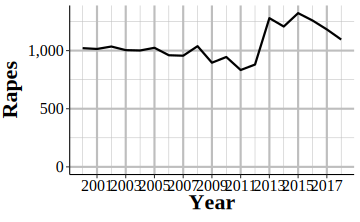
\includegraphics[width=1\linewidth,height=1\textheight]{03_offenses_known_files/figure-latex/rapePhilly-1} 

}

\caption{The annual number of rapes reported in Philadelphia, San Francisco, New York City, and Jackson, MS, 2005-2019.}\label{fig:rapePhilly}
\end{figure}

In comparison, New York City has the sudden spike a year
later, which indicates that they did not start using the new
definition until 2014. Figure \ref{fig:rapeNYC} shows that
rape is fairly steady, though increasing, in the years
leading up to 2013 and has almost no change from 2012 to
2013, but a huge increase in 2014 and then steadily
increases from there, spiking again in 2018. This seems like
a fairly clear indicator that NYC simply did not follow the
new definition until 2014.

Less clear is what is happening in San Francisco, shown in
Figure \ref{fig:rapeLA}. Here we do see an increase in 2013
which while it appears small on the graph is actually a 49\%
increase from 2012. Then there is a much larger spike in
2014 - a 120\% increase - which may suggest that part of the
agency started following the new definition in 2013 and the
remainder followed in 2014. Or maybe some months used the
old definition and others the new definition in 2013, while
all of 2014 used the new definition However, increases or
decreases are relatively common in San Francisco so it could
also be that the agency only switched to the new definition
in 2014 and the spike in 2013 is just a coincidence.

Finally, we will look at Jackson Police Department in
Mississippi where the definition change seems to have had no
effect. As seen in Figure \ref{fig:rapeJackson}, reported
rapes start to undulate in 2010 with 2013 data perfectly in
line with the before and after trends - no sign that there
is a change in reporting. This suggests that Jackson simply
did not follow the definition change and continues to report
using the old definition.

My takeaway from this is that rape should not be used at all
for years after 2012. While the definition change makes
pre-2013 and 2013+ years non-comparable, the differences in
agency responses to this change - i.e.~if they follow the
rules or not - is such a mess that the data is too flawed to
use.

\subsection{The decline of
manslaughter}\label{the-decline-of-manslaughter}

This data contains two different crime subcategories for
homicide: ``murder and non-negligent manslaughter,'' and
``manslaughter by negligence.'' The first is our measure of
murder, and it includes everything we traditionally think of
when it comes to murder - shootings, stabbings,
strangulation, basically any intentional killing of another
person.\footnote{Attempted murder is usually classified as
  an aggravated assault.} Suicides, killing a fetus, and
accidental killings (e.g.~car crashes) are not considered
murders.\footnote{Even the intentional killing of a fetus is
  classified as an aggravated assault against the mother,
  not a murder of the fetus.} The second, manslaughter by
negligence - usually called just ``manslaughter'' - is when
someone kills another person through ``gross negligence''
but does not kill them intentionally. This can include
accidental killings when the death was caused by gross
negligence. The FBI provide examples of this as kids playing
with guns and shooting each other (and not knowing the gun
was loaded) or a hunter accidentally shooting someone while
hunting. After the late 1970s this excludes deaths from
traffic accidents caused by negligence, such as hit and runs
or DUIs. However, prior to this, these deaths were included,
which is the cause of the very high number of manslaughters
in the 1960s and 1970s.

Figure \ref{fig:manslaughterVsMurder} shows the annual
number of murders, manslaughters, and the sum of the two
nationwide from 1960-2022. This just sums up the total
reported counts from every agency each year so part of the
increase is simply due to more agencies reporting as the
year gets closer to the present day - so please pay
attention to the diverging paths of each crime, not the
trend for the individual crime over time. Murder is always
more common than manslaughter, but these values are not that
far apart in the early decade of data and manslaughter does
not become rare until the end of the 1970s.

\begin{figure}

{\centering 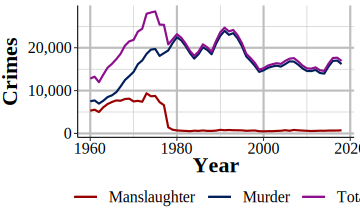
\includegraphics[width=1\linewidth,height=1\textheight]{03_offenses_known_files/figure-latex/manslaughterVsMurder-1} 

}

\caption{The annual number of murder and non-negligent manslaughter, manslaughter by negligence, and the sum of the two, nationwide from 1960-2022.}\label{fig:manslaughterVsMurder}
\end{figure}

Figure \ref{fig:manslaughterPercent} shows another way to
look at this data: manslaughter as a percent of reported
murder. In the early years of our data manslaughter was
fairly common, with about 70-80\% as many manslaughters
reported as murders. This declined sharply in the mid-1960s
until there were around 45\% as many manslaughters as
murders in the mid-1970s. Again, this declined until it was
about 4\% in 1980, and it has remained around there ever
since. As police behavior could reduce traffic fatalities -
and arrests for DUIs and traffic tickets are designed to
improve public safety - it is unfortunate the we no longer
have data on traffic deaths.

Manslaughter increased to over 1,000 for the first time
since 1978 in 2020, increased against to over 1,700 in 2021
and continued at around that number in 2022. This is
possibly related to the increase in murders over the last
few years of available data. Unfortunately, this dataset
does not allow us to do almost anything at figuring out more
information than monthly or annual counts. NIBRS, in
comparison, allows us to do this kind of deep dive, and for
curious readers NIBRS also has manslaughter so you can
investigate this question yourself.

\begin{figure}

{\centering 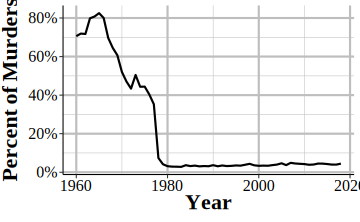
\includegraphics[width=1\linewidth,height=1\textheight]{03_offenses_known_files/figure-latex/manslaughterPercent-1} 

}

\caption{Reported manslaughter by negligence as a percent of reported murder and non-negligent manslaughter, nationwide 1960-2022.}\label{fig:manslaughterPercent}
\end{figure}

\chapter{Property Stolen and Recovered (Supplement to Return
A)}\label{stolen_property}

The Property Stolen and Recovered dataset, also known as the
Supplement to Return A\footnote{Return A being another name
  for the Offenses Known and Clearances by Arrest dataset.},
tracks monthly data on property crimes (theft, burglary,
robbery, and motor vehicle theft), with information on where
the crime occurred, what was stolen, and the estimated value
of the stolen property. The ``recovered'' part of this
dataset covers the type and value of property recovered.
Like most other SRS datasets this is at the agency-month
level so you can, for example, learn how often burglaries
occur at the victim's home during the day, and if that rate
changes over the year or differs across agencies. The data,
however, provides no information about the offender or the
victim (other than if the victim was an individual or a
commercial business \footnote{Based on the location of the
  incident - ``bank'', ``gas station'', etc.}).

The value of stolen property is generally based on the
victim's estimate. However, police are supposed to use the
market value for items, even if that value is different than
the victim's estimate. Because of this, the reported values
should be treated as rough estimates. And since this is the
victim's reporting it may be incomplete. For example, say a
person was burglarized and had 10 of their possessions
stolen but they only realized that nine items were taken.
They would report these nine items to the police but the
tenth item would be left out of our data.

This dataset provides a rough estimate of the cost of crime,
limited to the value of stolen property. It excludes other
important costs such as physical injuries, emotional harm,
or preventative expenses (e.g., home security systems). For
some types of stolen property we also know the number of
offenses that occurred meaning that we can use both of these
numbers to create an average value of stolen property per
offense. An issue here is that we only have the monthly
number of offenses and monthly value of the property. We can
make the average value per offense but will not know if our
average is affected by having an outlier in the data - such
as one theft of an extremely expensive item.

Before getting into the details of this data, let us look at
one example of how this data can measure property crime in a
few different ways, and look at common pitfalls. We will
look at home burglaries that occur during the day in
Philadelphia. Figure \ref{fig:phillyHomeBurglaryCount} shows
the annual number of daytime home burglaries Philadelphia
and in recent years it has declined sharply into having the
fewest on record in 2020 followed by a very low number of
crimes in 2021 and 2022. So citywide, Philadelphia has never
been safer (averaging across the last few years) when it
comes to the number of daytime home burglaries. As you
should be aware by this point in the book, SRS data is
optional and not all agencies report data every year.

In this case, 2019-2021 data are all partial-year reports,
with only 9, 4, and 9 months, respectively, reported for
these years. Every previous year other than 1974, 1975,
1988, and 1989\footnote{1974 had11 months, 1975 had 9
  months, 1988 had 10 months, and 1989 had 11 months of
  data.} had a full 12-months of data reported. So it makes
sense the 2019-2021 had fewer crimes if they only submitted
data for part of the year. This is something that is pretty
obvious - you cannot compare 12 months of data with
\textless12 months of data - but it is a common mistake so
you should check how many months are reported every time you
compare multiple years.

\begin{figure}

{\centering 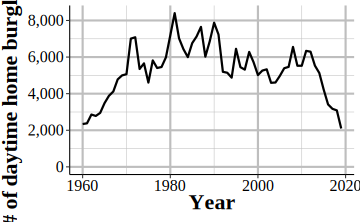
\includegraphics[width=1\linewidth,height=1\textheight]{04_stolen_property_files/figure-latex/phillyHomeBurglaryCount-1} 

}

\caption{The annual number of daytime home burglaries reported in Philadelphia, PA, 1960-2022.}\label{fig:phillyHomeBurglaryCount}
\end{figure}

When considering the cost of crime, we also want to know the
actually monetary cost of that incident. Figure
\ref{fig:PhillyBurglaryCost} measures this cost of crime by
showing the annual value of the property stolen for daytime
home burglaries in Philadelphia. The years without 12 months
of data are excluded from the figure. Like many variables in
this dataset, there is no reported crime value until 1964,
so the data shows a value of 0 from 1960-1963.

The trend here is different than the previous graph which
showed movement in the number of burglaries but not major
trend changes until the 2010s; here is a steady increase
over the long term, though with varying speed of increase,
until it peaked in the late 2000s/early 2010s before
declining substantially in recent years. While the number of
burglaries peaked in the early 1980s, the total value of
burglaries did not peak until the early 2010s, so the cost
of this crime (even this very narrow measure of cost) cannot
be ascertained from knowing the number of burglaries alone.
From this measure we can say that daytime home burglaries
were worse in the early 2010s and are substantially better
currently.

\begin{figure}

{\centering 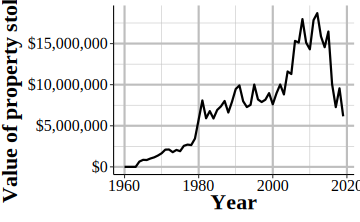
\includegraphics[width=1\linewidth,height=1\textheight]{04_stolen_property_files/figure-latex/PhillyBurglaryCost-1} 

}

\caption{The total annual cost of daytime home burglaries in Philadelphia.}\label{fig:PhillyBurglaryCost}
\end{figure}

The final way we can measure daytime home burglaries is to
put the previous variables together to look at the cost per
burglary. This will give us the average amount of property
stolen from each burglary victim. Figure
\ref{fig:phillyHomeCostPerBurglary} shows the average cost
per burglary for each year of data available. Now we have a
different story than the other graphs. Even though the
number of daytime home burglaries declined substantially
over the last decade and the total cost is around the level
seen in the 1980s, the cost per burglary remains high in
recent years, though down from the peak in the mid-2010s.
This suggests that while burglaries are down, the burden on
each burglary victim has continued to grow.

A perhaps obvious issue here is that we have no way to
determining how much outliers are affecting results. If one
year has, for example, a home burglary where \$10 million
worth of jewelry is stolen then that year's total value of
property stolen would be much higher just due to a single
burglary. There is, unfortunately, no way to handle this in
this dataset, though NIBRS has similar data which does allow
you to check for outliers.\footnote{Having an outlier, as
  long as it is not just a data entry error, should not
  necessarily mean you remove it. If we removed rare events
  after all we would have to drop murders from our data as
  murders are very uncommon crimes.}

\begin{figure}

{\centering 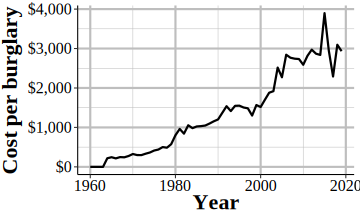
\includegraphics[width=1\linewidth,height=1\textheight]{04_stolen_property_files/figure-latex/phillyHomeCostPerBurglary-1} \includegraphics[width=1\linewidth,height=1\textheight]{04_stolen_property_files/figure-latex/phillyHomeCostPerBurglary-2} 

}

\caption{The annual cost per burglary for daytime home burglaries in Philadelphia, 1960-2022.}\label{fig:phillyHomeCostPerBurglary}
\end{figure}

Part of this - and part of the long-term increase seen in
Figure \ref{fig:PhillyBurglaryCost} - is simply due to
inflation. A dollar in 1964, the first year we have data on
the value of burglaries, is worth \$9.84 in 2023, according
to the Bureau of Labor Statistics.\footnote{Based on June of
  both years} The values in this data are \emph{not}
adjusted for inflation so you need to do that adjustment
yourself before any analyses, otherwise your results will be
quite a bit off. When we adjust all values to 2023 dollars,
as shown in Figure
\ref{fig:phillyHomeCostPerBurglaryInflation}, the trend
becomes changes a bit. There's still a steady increase in
cost per burglary over time but it is far more gradual than
in Figure \ref{fig:phillyHomeCostPerBurglary}. And now the
difference from the cost in early years and late years are
far smaller.

\section{Agencies reporting}\label{agencies-reporting}

The data is available from 1960 to the present, though
olders years of data have fewer variables reported. Figure
\ref{fig:propertyAgencies} show the number of agencies each
year that reported at least one month during that year. In
the first several years of data barely any agencies reported
data and then it spiked around 1966 to over 6,000 agencies
per year then grew quickly until over 12,000 agencies
reported data in the late 1970s. From here it actually
gradually declined until fewer than 12,000 agencies in the
late 1990s before reversing course again and growing to
about 15,000 agencies by 2019 - down several hundred
agencies from the peak a few years earlier. We see the
now-typical drop in 2021 as a result of the FBI's death of
SRS and then the partial recovery in 2022 when SRS was
reborn. The agencies that still reported in 2021 did so by
reporting NIBRS data which the FBI converted to this format.

\begin{figure}

{\centering 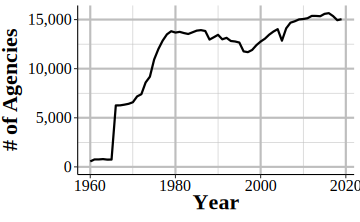
\includegraphics[width=1\linewidth,height=1\textheight]{04_stolen_property_files/figure-latex/propertyAgencies-1} 

}

\caption{The annual number of police agencies that report at least month of data and 12 months of data that year.}\label{fig:propertyAgencies}
\end{figure}

Since this data is called the ``Supplement to Return A'' we
would expect that the agencies that report here are the same
as the ones that report to the Offenses Known and Clearances
by Arrest data, which is also called the Return A dataset.
Figure \ref{fig:agenciesInBoth} shows the percent of
agencies in this dataset that are report at least one month
of Return A data. Except for the first several years of data
in the 1960s, we can see that most years have nearly all
agencies reporting to both, though this has declined
slightly in recent years. Since the late 1970s, over 90\% of
agencies that report to the Offenses Known data also report
to this dataset.

\begin{figure}

{\centering 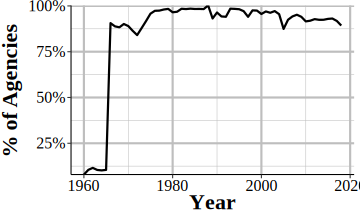
\includegraphics[width=1\linewidth,height=1\textheight]{04_stolen_property_files/figure-latex/agenciesInBoth-1} 

}

\caption{The percent of agencies in the Supplement to Return A data that report at least one month of data, and all 12 months of data, and are also in the Offenses Known and Clearances by Arrest (Return A) data in that year, 1960-2022.}\label{fig:agenciesInBoth}
\end{figure}

When filtering the data to agencies that report a full 12
months of both the Return A and the Supplement to Return A,
shown in Figure \ref{fig:agenciesInBoth12Month}, trends are
quite similar to Figure \ref{fig:agenciesInBoth} though now
the average percent is around 75\% rather than 90\%. This
translates to around 11k agencies though it drops starting
in 2018 until fewer than 8,500 agencies report full data to
both datasets in 2022.

\section{Important variables}\label{important-variables-1}

This data can really be broken into two parts: the monthly
number of property (as well as robbery) crimes that occur
that are more detailed than in the Offenses Known data, and
the value of the property stolen (and recovered) from these
crimes. For each category I present the complete breakdown
of the available offenses/items stolen and describe some of
the important issues to know about them. Like other SRS
data, there are also variables that provide information
about the agency - ORI codes, population under jurisdiction
- the month and year that the data covers, and how many
months reported data.

\subsection{A more detailed breakdown of property (and
robbery) crimes}\label{propertycount}

The first part of this data is just a monthly (or yearly if
you aggregate the data) number of crimes of each type
reported to the police and that a police investigation
discovered actually happened.\footnote{For more on this
  process, please see Section \ref{actual}}. There are six
crimes and their subsets included here: burglary, theft,
robbery, and motor vehicle theft. The remaining two are rape
and murder, but they do not break down these crimes into any
subcategories and are only available starting in 1974.

Though this data starts in 1960, not all variables are
available then. 1963 and 1964 saw many new variables added -
the values in these variables are reported as 0 in previous
years - and in 1974 and 1975 even more variables were added.
In 1963 the value of burglaries where the time of the
burglary was known, thefts broken down into categories based
on the value of property taken, thefts of car parts, theft
from cars, shoplifting, and ``other'' thefts was added to
the data. In the following year this data began including
the value of property stolen from burglaries where the time
of the burglary was unknown was added as well as thefts of
bicycles, from ``coin operated machines'' (i.e.~vending
machines), purse snatching, and pick pocketing. The value of
property stolen during rapes and murders was first reported
in 1974. Finally, 1975 was the last year with new variables,
with this year including consumable goods, stolen guns,
household goods, livestock, office equipment and
electronics, and sound and picture equipment.

The complete list of each subsection and a brief definition
for the non-obvious ones are presented below.

\begin{itemize}
\tightlist
\item
  Burglary

  \begin{itemize}
  \tightlist
  \item
    Home/residence during the day (6AM - 5:59PM)
  \item
    Home/residence during the night (6PM - 5:59AM)
  \item
    Home residence at unknown time
  \item
    Non-residence (i.e.~all buildings other than victim's
    home) during the day (6:00AM - 5:59PM)
  \item
    Non-residence (i.e.~all buildings other than victim's
    home) during the night (6:00PM - 5:59AM)
  \item
    Non-residence (i.e.~all buildings other than victim's
    home) at unknown time
  \end{itemize}
\item
  Theft/larceny (excluding of a motor vehicle)

  \begin{itemize}
  \tightlist
  \item
    Less than \$50
  \item
    \$50-\$199
  \item
    \$200 and up
  \item
    Pick pocket
  \item
    Purse snatching
  \item
    Shoplifting
  \item
    Stealing from a car (but not stealing the car itself)
  \item
    Stealing parts of a car, such as the car battery or the
    tires
  \item
    Stealing a bicycle
  \item
    Stealing from a building where the offender is allowed
    to be in (and is not counted already as shoplifting)
  \item
    Stealing from a ``coin operated machine'' which is
    mainly vending machines
  \item
    All other thefts
  \end{itemize}
\item
  Robbery

  \begin{itemize}
  \tightlist
  \item
    Highway - This is an old term to say a place is outside
    and in generally accessible and visible areas. This
    includes robberies on public streets and alleys.
  \item
    Commercial building - This is robberies in a business
    other than ones stated below. Includes restaurants,
    stores, hotels, bars.
  \item
    Gas station
  \item
    Chain/convenience store - a neighborhood store that
    generally is open late and sells food
  \item
    Home/residence
  \item
    Bank
  \item
    Miscellaneous/other - This is all other robberies not
    already covered.
  \end{itemize}
\item
  Motor vehicle theft

  \begin{itemize}
  \tightlist
  \item
    Stolen in current agency's jurisdiction and found by
    that agency
  \item
    Stolen in current agency's jurisdiction and found by
    another agency
  \item
    Stolen in another agency's jurisdiction and recovered by
    current agency
  \end{itemize}
\item
  Murder
\item
  Rape
\end{itemize}

Burglary is reported based on whether the building burgled
was the victim's residence or not, and also the time of the
burglary. Time is either during the day (6AM-5:59PM) or
night (6PM-5:59AM) or if the time is unknown. Data is
available since 1960 for both the day and night burglaries,
but only since 1964 for the unknown time burglaries. For
robbery, the subcategories are based on where the robberies
occurred such as if it happened in a bank, a gas station, or
a street.

Theft is divided into two groups. The first group is based
on the value of items stolen: less than \$50, \$50-\$199,
and \$200 and up. The second group of thefts is broken into
the type of theft such as a shoplifting or stealing from
someone's car. All theft variables begin in 1960 other than
thefts from a coin machine and from a building which start
in 1964 and the miscellaneous ``All other thefts'' variable
that has data starting in 1961. Finally, motor vehicle theft
is broken into where the stolen vehicle was stolen and
found: stolen in the reporting agency's jurisdiction and
found by the same agency, stolen in the reporting agency's
jurisdiction and found by a different agency, and stolen in
a different agency's jurisdiction and found by the reporting
agency.

The first group is a useful example of a problem in this
data, which can be seen happening in 1974. In Figure
\ref{fig:theftByValue} we use data from all agencies in the
United States that reported 12 months of data to see the
share of the total value of thefts by the three value
categories. Thefts of between \$50 and \$200 start as the
most common at nearly 60\% of thefts in 1960 and steadily
decline to under 20\% by 2022. Thefts of over \$200 increase
steadily from about 28\% of thefts in 1960 to almost 50\% in
1973 and then drop to 16\% in 1974. Then the share of thefts
over \$200 slowly increases over time to end our data at
over 55\% of thefts. Thefts valued at under \$50 have a near
mirror trend as over \$200, starting at under 15\% in 1960,
declining a bit after that and then massively spiking to
49\% in 1974 before starting a slow decline to 27\% in 2022.

\begin{figure}

{\centering \includegraphics[width=1\linewidth,height=1\textheight]{04_stolen_property_files/figure-latex/theftByValue-1} 

}

\caption{The annual breakdown in total theft value by the three value categories: less than \$50, \$50-\$199, and \$200 and over, among all agencies that reported 12 months of data in that year, 1960-2022.}\label{fig:theftByValue}
\end{figure}

What caused this weird swap of the less than \$50 and at
least \$200 values? Well, part of it is that different
agencies report over time so year-to-year comparisons are
not really appropriate. Even agencies that report every year
may report only some months of data. But we corrected that
by filtering the data shown in Figure \ref{fig:theftByValue}
to only agencies that reported 12 months of data.
Unfortunately, even doing that is not sufficient, as we can
see below.

Figure \ref{fig:theftByValueCalifornia} replicates Figure
\ref{fig:theftByValue} but now only for agencies in
California and zooms in to 1960-1980. In every agency in
California there were zero reported thefts under \$50
starting in 1969 and ending in 1974. The number of thefts
between \$50 and \$200, and thefts over \$200 increased,
suggesting that agencies still reported the data but in the
wrong category. Then in 1974 the thefts under \$50 were
reported once again and the number of thefts in the other
categories dropped. Given that the entire state changed
reporting practices I believe that this was from either a
policy at the state-level or some data error by the state
before they sent the data to the FBI. It certainly is not
true that there were zero thefts under \$50 for five years
in California.

Luckily in this case it was a fairly easy error to find -
though I suspect that California is only part of the
problem. But it reveals a broader issue with UCR data. The
purpose of the data is that it is ``Uniform,'' but we see
that entire states can stop reporting certain data even when
they say that they report data for all 12 months. Since UCR
data is voluntary, agencies can report some, all, or none of
the data, which makes it frustrating and time-consuming for
researchers to ensure that the results in the data are real
and not simply caused by reporting issues.

\begin{figure}

{\centering \includegraphics[width=1\linewidth,height=1\textheight]{04_stolen_property_files/figure-latex/theftByValueCalifornia-1} 

}

\caption{The annual breakdown in total theft value by the three value categories: less than \$50, \$50-\$199, and \$200 and over, among agencies in California that reported 12 months of data in that year, 1960-1980}\label{fig:theftByValueCalifornia}
\end{figure}

\subsection{The value of property
stolen}\label{the-value-of-property-stolen}

The next set of variables is the value of the property
stolen in each crime, as well as the value of property
stolen broken down by the type of property (e.g.~clothing,
electronics, etc.). To be clear, this is \emph{only} the
value of the property stolen during the crime. The cost of
any injuries (mental or physical) or any lasting cost to the
victim, their family, and society for these crimes are not
included. This, of course, vastly underestimates the cost of
these crimes so please understand that while this is a
measure of the cost of crime, it is only a narrow slice of
the true cost.

The cost is the cost for the victim to replace the stolen
item. So the current market price for that item (though
factoring in the current state the item is in, e.g.~if it is
already damaged) and, for businesses, the cost to buy that
item and \emph{not} the cost they sell it for. While the
police can ask the victim how much the property was worth,
they are not required to use the exact amount given as
victims may exaggerate the value of items. This is not an
exact science, so I recommend only interpreting these values
as estimates - and potentially rough estimates. None of this
data is adjusted for inflation so if you are comparing
values over time you will need to do that adjustment
yourself.

The value of the property stolen is broken into two
overlapping categories: by crime type, and by type of
property that was stolen. These are the exact same
categories as covered in Section \ref{propertycount} but now
is the dollar amount of the items stolen from those types of
crimes. The second group is what type of item, based on
several discrete categories, was stolen. Please note that
multiple items can be stolen in each category and this data
counts the property stolen for each crime type \emph{as well
as} for each item type. So if you sum up all of the crime
variables and all of the item type variables together you
will over-count the value of property stolen. Each of the
categories and their definitions are detailed below.

Some of these will overlap with the list in the previous
section, though for completeness I will repeat them.

Here are the subsets of crimes:

\begin{itemize}
\tightlist
\item
  Burglary

  \begin{itemize}
  \tightlist
  \item
    Home/residence during the day (6:00am - 5:59pm)
  \item
    Home/residence during the night (6:00pm - 5:59am)
  \item
    Home residence at unknown time
  \item
    Non-residence (i.e.~all buildings other than victim's
    home) during the day (6:00am - 5:59pm)
  \item
    Non-residence (i.e.~all buildings other than victim's
    home) during the night (6:00pm - 5:59am)
  \item
    Non-residence (i.e.~all buildings other than victim's
    home) at unknown time
  \end{itemize}
\item
  Theft/larceny (excluding of a motor vehicle)

  \begin{itemize}
  \tightlist
  \item
    Less than \$50
  \item
    \$50-\$199
  \item
    \$200 and up
  \item
    Pick pocket
  \item
    Purse snatching
  \item
    Shoplifting
  \item
    Stealing from a car (but not stealing the car itself)
  \item
    Stealing parts of a car, such as the car battery or the
    tires
  \item
    Stealing a bicycle
  \item
    Stealing from a building where the offender is allowed
    to be in (and is not counted already as shoplifting)
  \item
    Stealing from a ``coin operated machine'' which is
    mainly vending machines
  \item
    All other thefts
  \end{itemize}
\item
  Robbery

  \begin{itemize}
  \tightlist
  \item
    Highway - This is an old term to say a place is outside
    and in generally accessible and visible areas. This
    includes robberies on public streets and alleys.
  \item
    Commercial building - This is robberies in a business
    other than ones stated below. Includes restaurants,
    stores, hotels, bars.
  \item
    Gas station
  \item
    Chain/convenience store - a neighborhood store that
    generally is open late and sells food
  \item
    Home/residence
  \item
    Bank
  \item
    Miscellaneous/other - This is all other robberies not
    already covered.
  \end{itemize}
\item
  Motor vehicle theft

  \begin{itemize}
  \tightlist
  \item
    Stolen in current agency's jurisdiction and found by
    that agency
  \item
    Stolen in current agency's jurisdiction and found by
    another agency
  \item
    Stolen in another agency's jurisdiction and recovered by
    current agency
  \end{itemize}
\item
  Murder
\item
  Rape
\end{itemize}

And here are the items stolen:

\begin{itemize}
\tightlist
\item
  Currency

  \begin{itemize}
  \tightlist
  \item
    This includes all money and signed documents that can be
    exchanged for money (e.g.~checks). Blank checks and
    credit and debit cards are not included (they are in the
    Miscellaneous/other category)
  \end{itemize}
\item
  Jewelry and ``precious metals''

  \begin{itemize}
  \tightlist
  \item
    Only metals that are considered high value are included
    here. Metals that are generally worth little are counted
    in the Miscellaneous/other category.
  \end{itemize}
\item
  Clothing and fur

  \begin{itemize}
  \tightlist
  \item
    This also includes items that you take with you when
    leaving the house (except for your phone): wallet,
    shoes, purse, backpacks.
  \end{itemize}
\item
  Motor vehicle stolen in current agency's jurisdiction

  \begin{itemize}
  \tightlist
  \item
    This includes only vehicles than can be driven on wheels
    so excludes trains and anything on water or that can
    fly.
  \end{itemize}
\item
  Office equipment and electronics

  \begin{itemize}
  \tightlist
  \item
    This includes ``typewriters'' and ``magnetic tapes'' but
    is essentially any kind of equipment needed to run a
    business. So printers, computers, cash registers,
    computer equipment like a monitor or a mouse, and
    computer software. These items do not have to be stolen
    from a commercial building to be included in this
    category.
  \end{itemize}
\item
  Sound and picture equipment

  \begin{itemize}
  \tightlist
  \item
    This is a kind of odd category that is a product of its
    time. Anything that produces noise or pictures
    (including the fancy motion pictures) is included. This
    includes TVs, cameras, projectors, radios, MP3 players
    (but not phones that can play music) and (since again,
    this is a very old dataset) VHS cassettes.
  \end{itemize}
\item
  Guns

  \begin{itemize}
  \tightlist
  \item
    This includes all types of firearms other than toys or
    BB/pellet/paintball guns (which are in the
    ``Miscellaneous/other'' category).
  \end{itemize}
\item
  Home furniture

  \begin{itemize}
  \tightlist
  \item
    This includes all of the ``big things'' in a house:
    begs, chairs, AC units, washer/dryer units, etc.
    However, items that are in the ``Office equipment and
    electronics'' category do not apply.
  \end{itemize}
\item
  Consumable goods

  \begin{itemize}
  \tightlist
  \item
    This is anything that can be consumed such as food,
    drinks, and drugs, or anything you use in the bathroom.
  \end{itemize}
\item
  Livestock

  \begin{itemize}
  \tightlist
  \item
    This is all animals other than ones that you would
    consider a pet
  \end{itemize}
\item
  Miscellaneous/other

  \begin{itemize}
  \tightlist
  \item
    Anything that is not part of the above categories would
    fall in here. Cell phones and credit cards are included.
  \end{itemize}
\end{itemize}

\subsection{Value of recovered property by type of item
stolen}\label{value-of-recovered-property-by-type-of-item-stolen}

For a subset of items (listen below), this data includes the
value of the items that were recovered. The only information
we have for the value of recovered property is for the
breakdown in the items themselves - not breakdowns of crimes
such as robbery or burglary. So we can know the value of
guns recovered, but not if those guns were taken from a
burglary, a robbery, a theft, etc.

While this dataset began in 1960, the recovered property
variables begin later, and in different years. For clothing
and fur, currency, jewels and precious metals, motor
vehicles, miscellaneous/other, and the variable that sums up
all of the recovered property variables, the first year with
data was 1961. The remaining variables - consumable goods,
guns, household goods/home furniture, livestock, office
equipment and electronics, and sound and picture equipment -
began in 1975.

Another issue is that it uses the value of the property as
it is recovered, not as it is stolen. For example, if
someone steals a laptop that is worth \$1,000 and then the
police recover it damaged and it is now worth only \$200, we
would see \$1,000 for the stolen column for ``office
equipment and electronics'' and only \$200 for the recovered
column for that category. So an agency that recovers 100\%
of the items that were stolen can appear to only recover a
fraction of them since the value of recovered items could be
substantially lower than the value of stolen items.
Therefore, there is a systematic bias in the data that shows
a lower recovery value than stolen value in many cases. It
is extremely unlikely that an item would be worth more when
the police recover it than when it was stolen.

Unfortunately there is no way to know how many items are
actually recovered (except for motor vehicles), only the
value of the recovered property.\footnote{Even if we look at
  the Offenses Known and Clearances by Arrest data, that
  only says if there was an arrest or exceptional clearance
  in the case, not if the property stolen was recovered} For
these reasons I recommend against using this variable to try
to measure a recovery rate.

The full list of items recovered are below:

\begin{itemize}
\tightlist
\item
  Currency
\item
  Jewelry and ``precious metals''
\item
  Clothing and fur
\item
  Motor vehicle stolen in current agency's jurisdiction
\item
  Office equipment and electronics
\item
  Sound and picture equipment
\item
  Guns
\item
  Household goods/Home furniture
\item
  Consumable goods
\item
  Livestock
\item
  Miscellaneous/other
\end{itemize}

\section{Data errors}\label{data-errors}

This dataset comes with a considerable number of data errors
- basically enormous valuations for stolen
property.\footnote{Since the minimum value is 0 there is
  less chance of data errors underestimating the value of an
  item, though some errors must certainly occur.} Some of
the values are so big that it is clearly an error and not
just something very expensive stolen. Unfortunately we can't
just assume that high values are always errors. For example,
say someone stole an extremely expensive car in a city with
otherwise very little stolen property. We'd see a huge spike
in the value of stolen property which may appear to be an
error but would in fact be real.

Some of the stolen property include variables for both the
number of items of that type stolen and the total value of
the items. From this we can make an average value per item
stolen which can help our understanding of what was stolen.
However, some items only have the value of the property
stolen and the value of property recovered so we do not know
how many of those items were stolen. These cases make it
even harder to believe that a large value is true and not
just a data error since we do not know if the number of
these crimes increased, causing the increase in the value
reported. We will look at a couple examples of this and see
how difficult it can be to trust this data.

First, we will look at the value of livestock thefts in New
York City. Livestock is one of the variables where we know
the value stolen and recovered but not how many times it
happened. Being a major urban city, we might expect that
there are not many livestock animals in the city so the
values should be low. Figure \ref{fig:nycLivestock} shows
the annual value of livestock thefts in NYC. There are two
major issues here. First, in all but two years they report
\$0 in livestock thefts. This is likely wrong since even New
York City has some livestock (even just the police horses
and the horse carriages tourists like) that probably got
stolen. The second issue is the massive spike of reported
livestock theft value in 1993 with over \$15 million stolen
(the only other year with reported thefts is 1975 with
\$87,651 stolen). Clearly NYC did not move from \$0 in
thefts for decades to \$15 million in a year and then \$0
again so this appears to be a blatant data error.

\begin{figure}

{\centering 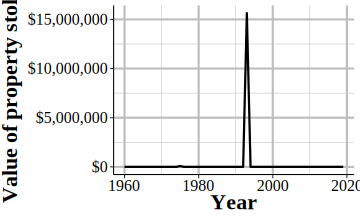
\includegraphics[width=1\linewidth,height=1\textheight]{04_stolen_property_files/figure-latex/nycLivestock-1} 

}

\caption{The annual value of stolen livestock in New York City, 1960-2022.}\label{fig:nycLivestock}
\end{figure}

It gets harder to determine when a value is a mistake when
it is simply a big spike - or drop - in data that otherwise
looks correct. Take, for example, the annual value of stolen
clothing and fur in Philadelphia from 1960-2019, shown in
Figure \ref{fig:phillyFurValue}. The annual value of these
stolen items more than doubled in 1989 compared to the
previous year and then declined rapidly in the following
year.

Is this real? Is it a data error? It is hard to tell. Here
we do not know how many clothing/fur thefts there were, only
the value of the total thefts that month (which is
aggregated annually here). It continues a multi-year trend
of increasing value of thefts but it is larger than previous
increases in value. And while the spike is very large in
percent terms, it is not so extraordinarily huge that we
immediately think it is an error - though some outlier
detection methods may think so if it is beyond the expected
value for that year.

Philadelphia had several years in this time period where
only part of that year's data was reported. In fact both
1988 and 1989 had fewer than 12 months of data; as did 1974
and 1975. So the year with fewer than 12 months had an
atypically high value of clothing and fur stolen. Normally
we would expect less data to lead to smaller numbers. But
that is not always true. Sometimes less data is a sign that
there is something wrong with the data quality altogether
and that we need to be cautious of any value in that year.
And even though we know that some years are missing months
of data just looking at this figure it is not clear which
years those are. So while graphing data helps, it is only by
looking at the data itself - and yes, this means you will
likely need to pull out a programming language like R or
python, or at the very least use Excel - and look at each
data point before trusting this data.

It is also important to have some understanding of what the
data \emph{should} look like when trying to figure out what
data point may be incorrect. In this figure we see a huge
spike in 1989. If we know, for example, that a ring of fur
thieves were active this year, then that makes it far more
likely that the data is real. This may be a rather odd
example, but it is helpful to try to understand the context
of the data to better understand when the ``weird'' data is
an error and when it is just ``weird but right.''

\begin{figure}

{\centering 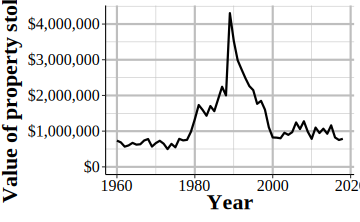
\includegraphics[width=1\linewidth,height=1\textheight]{04_stolen_property_files/figure-latex/phillyFurValue-1} 

}

\caption{The annual value of stolen clothing and fur in Philadelphia, PA, 1960-2019}\label{fig:phillyFurValue}
\end{figure}

Finally, some errors are so extreme that it is surprising
they were not captured during any of the review points from
the police officer entering data in their agency's computer
to the FBI releasing this data to the public. For example,
Figure \ref{fig:romeBicycles} shows Rome, New York, a city
of about 32,000 people in central New York State. Here's
what the reported value of bicycles stolen was for Rome in
our data.\footnote{For this example we would not worry about
  years where \textless12 months of data were reported.}

2020 had a bit of a spike in their stolen bicycle value,
from less than \$10,000 is the previous few years to over
\$5 billion. Yes, that is billion with a ``b.'' 2021
followed by slightly under \$3 billion worth of bicycles
stolen. In both years 19 bicycles were reported stolen.

Bicycles were not the only thing stolen in Rome. Consumable
goods such as food and toiletries were stolen to the tune of
\$5 billion in 2020 and \$1 billion in 2022, with only
\$84,278 worth of goods stolen in 2021. To put this into
perspective - not that it is needed - the total amount of
property stolen by theft the United States during 2019,
according to this dataset, was \$8 billion. Rome, NY,
superseded that by far just through two groups of property
stolen in 2020.

Now, obviously this is not real. This is just an error with
the police entering in the wrong price. But the issue is
that through all the layers of checks that occurred - checks
by the local police, by the state UCR system (though some
agencies submit directly to the FBI) and the FBI themselves
- failed to prevent this incorrect data from being
published. This is an obvious, glaring error. If this
slipped through the cracks, what less glaring issue did too?
So you cannot just trust that this data is right. You need
to check and recheck\footnote{and check again.} everything
before using it. This is the right approach for all data,
and especially for this data.

\begin{figure}

{\centering \includegraphics[width=1\linewidth,height=1\textheight]{04_stolen_property_files/figure-latex/romeConsumable-1} 

}

\caption{The annual value of stolen consumable goods, bicycles, livestock, and thefts from pickpocketing, in Rome, New York, 1960-2022.}\label{fig:romeConsumable}
\end{figure}

The Property Stolen and Recovered dataset offers a useful,
though imperfect, view of property crimes and their
financial impact. While limitations such as reporting gaps
and data inconsistencies exist, careful analysis can still
reveal important trends in the types and values of stolen
and recovered property. Researchers should approach this
data with caution, especially when making year-to-year
comparisons or analyzing categories with significant
outliers.

\chapter{Arrests by Age, Sex, and Race}\label{arrests}

The Arrests by Age, Sex, and Race dataset (ASR)\footnote{Sometimes
  called Arrests by Age, Sex, Race, and Ethnicity.} provides
monthly counts of arrests broken down by age, sex, and race
for a variety of crimes. This data includes a broader number
of crime categories than the crime dataset (the Offenses
Known and Clearances by Arrest data) though is less detailed
on violent crimes since it does not breakdown aggravated
assault or robberies by weapon type as the Offenses Known
data does.

For each crime it says the number of arrests for each
sex-age group with younger ages (15-24) showing the
arrestee's age to the year (e.g.~age 16, age 17) and other
ages grouping years together (e.g.~age 25-29, 30-34, ``under
10''). It also breaks down arrests by race-age by including
the number of arrestees of each race (American Indian,
Asian, Black, and White are the only included races) and if
the arrestee is a juvenile (\textless18 years old) or an
adult. The data does technically include a breakdown by
ethnicity-age (e.g.~juvenile-Hispanic,
juvenile-non-Hispanic) but almost no agencies report this
data and most do not report ethnicity at all. So in practice
the data does not include ethnicity. As the data includes
counts of arrestees, people who are arrested multiple times
are included in the data multiple times; it is not a measure
of unique arrestees.

\section{Agencies reporting}\label{agencies-reporting-1}

This data is available from 1974 through 2022 though after
2020 the measure for how many months of data an agency
reported changed so post-2020 data is difficult to compare
to 2020 and earlier.\footnote{Post-2020 years do have
  considerably fewer agencies reporting than in previous
  years.} Figure \ref{fig:arrestsAgenciesReporting} shows
how many agencies reported at least one month of the year
and every month of the year for 1974-2020.

The first year of data has about 9,000 agencies reporting at
least one month and that increases strongly to a little over
13,000 in the late 1970s, staying fairly steady until
decreasing in the late 1980s then increasing in the 2000s
until approximately 15,000 agencies report. The number of
agencies reporting 12 months of data follows a similar
trend, but at a lower level with about 4,000 fewer agencies
each year. This 15,000, however, still remains under the
estimated 18,000 police agencies in the United States and
below the reporting rates of UCR data such as the Offenses
Known and Clearances by Arrest data. This data is also
missing some important cities such as New York City which
has not reported even a single month since 2002 and Chicago
which tends to only report a single month if at all.

\begin{figure}

{\centering 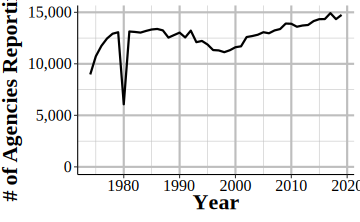
\includegraphics[width=1\linewidth,height=1\textheight]{05_arrests_files/figure-latex/arrestsAgenciesReporting-1} 

}

\caption{The annual number of agencies reporting at least one month of data and 12 months of data in that year.}\label{fig:arrestsAgenciesReporting}
\end{figure}

\section{What is an arrest? (what unit is this data
in?)}\label{what-is-an-arrest-what-unit-is-this-data-in}

This dataset counts each arrest separately, meaning that
individuals who are arrested multiple times will be counted
multiple times. It reports the most serious crime for each
arrest incident, so if someone commits multiple crimes
during an incident, only the most serious one is recorded.
Consider for example, a person who robs a bank, shooting and
killing a guard and pointing their gun at other people in
the bank. They are arrested and then released from jail
(just imagine that this is true) and are then arrested the
next day for shoplifting. And let us further assume that
both arrests were in the same month in the same agency. How
many arrests are here? They committed multiple crimes in the
first incident (murder, robbery, aggravated assault) but in
this dataset they would only be classified as an arrest for
the most serious crime, murder. And then separately they
would also be an arrested for shoplifting. So assuming that
no other arrests occurred in that police agency that month,
there would be two arrests reported: one for murder and one
for shoplifting.

There's no way to tell how many unique people were arrested,
or of those arrested multiple times which crimes they were
arrested for. So if you have 100 arrests there may be 1
person arrested 100 times or 100 people arrested once -
though, of course, the true number is likely somewhere in
between. This means that studies that try to use this data
as a measure of unique people or even the percent of
arrestees by group (age, sex, or race) relative to some base
rate of the population such as the number of people living
in that city are going to be wrong - though how wrong is
unclear.

Common uses of this data - more common in more news articles
or advocacy group reports than in peer-reviewed research
articles - compare the percent of arrestees of a certain
group to the percent of a city's population of that group.
Any differences between the arrestee percent and the
resident percent is, according to these reports, evidence of
a disparity. This is most common for looking at differences
by race.\footnote{Disparity, of course, does not even mean
  discrimination.} For example, say a city is equally split
between Black and White residents (and no other races are
present, for the simplicity of this example). If
\textgreater50\% of arrestees for a particular crime are
Black, that is often cited as evidence of anti-Black
discrimination.

There are two assumptions built into this. First, that
offending rates are identical between Black and White
residents; second, that reoffending rates are identical. If,
for example, Black people in this example commit that crime
at higher rates than White people then all else being equal
you would expect this group to have a higher share of
arrests than their share of the resident population. Second,
it assumes that people of each race are rearrested at
similar rates. Put another way, it assumes that if 100 Black
people are arrested and 100 White people are arrested, there
are an equal number of unique people in each group. If these
assumptions are violated - and they certainly are violated
to some degree in every use of the data - the conclusions
will be wrong. Whether this distinction between arrests and
unique people arrested affects your interpretation of the
data depends on the study you are doing, but it is important
to consider in your research. One way to address this is to
use other data on the rate of rearrest by group, though you
would have to be very careful to not extrapolate the results
of the other study too far beyond what they could tell you
about the specific time and place they studied.

Another solution would be to try to bound results, such as
calculating how extreme your assumptions (e.g.~assuming how
different the true offense rates between races are) can be
for your conclusions to still hold. Going back to the
example of a city with 50\% White and 50\% Black people, say
that there are 10 arrests with a split of 1 White and 9
Black arrestees. If offense rates are identical you would
expect 5 White and 5 Black people arrested, not a disparity
of 9 to 1. So you could say that this disparity is
reasonable if the Black people commit this offense at a rate
of nine times as often than White people.\footnote{This is a
  simplification as there are other things that affect
  arrests such as witness cooperation, details of the
  offense like time of day and location, and (especially in
  the case of rare events like only 10 arrests) random
  chance.}

Is this bounding assumption reasonable? In this context-less
example, I have no idea. There certainly may be cases where
it is reasonable but that is context dependent. And you need
to understand the context of what you are studying. Numbers
are not enough. If based on your understanding of the
context of what you are studying you believe that it is
unreasonable that Black people commit that offense at a rate
nine times that of White people, then you may conclude that
the disparity is not explained by differences in offending
rates. Your next step is to identify another explanation and
try to rule that out too.

\subsection{The Hierarchy Rule}\label{the-hierarchy-rule}

The Hierarchy Rule is used in this data which means that
when someone is arrested for multiple crimes, only the most
serious crime is recorded. For example, if a person commits
murder, robbery, and theft, only the murder is reported.
Essentially, the FBI chose seven crimes in 1929 that they
call Index Crimes - or sometimes called Part I crimes - and
these were considered the most important crimes to be
recorded.\footnote{Partly based on the quality of the data
  available as they considered these crimes to be a good
  combination of well-reported and serious.} If a person is
arrested for multiple crimes and an Index Crime is one of
those crimes, then the Index Crime at the top of the
Hierarchy is the one recorded in this data. Below I have
listed all crimes included in this dataset and the crimes
1-7 as well as 9 (arson) are the Index Crimes. The top of
the Hierarchy is the crime with the lowest number. So murder
is always reported in incidents where there is a murder;
rape is always reported when there is an incident with rape
but no murder; etc.

The remaining crimes - the ones that are not Index crimes -
are called Part II crimes and are not arranged in any
particular way. So a lower value numbered crime is not
higher on the Hierarchy than a higher value number - Part II
crimes do not follow the Hierarchy. If all of the crimes in
an incident are Part II crimes then the agency must decide
for themselves which crime is the most serious. This can
lead to agencies deciding their own hierarchy differently
than others which makes this data much less comparable
across agencies than if there was a standard
rule.\footnote{This here is another example of where the
  ``Uniform'' part of Uniform Crime Reporting is more of a
  suggestion than a rule.}

\begin{enumerate}
\def\labelenumi{\arabic{enumi}.}
\tightlist
\item
  Homicide
\end{enumerate}

\begin{enumerate}
\def\labelenumi{\alph{enumi}.}
\tightlist
\item
  Murder and non-negligent manslaughter
\item
  Manslaughter by negligence
\end{enumerate}

\begin{enumerate}
\def\labelenumi{\arabic{enumi}.}
\setcounter{enumi}{1}
\tightlist
\item
  Rape
\item
  Robbery
\item
  Aggravated assault
\item
  Burglary
\item
  Theft (other than of a motor vehicle)
\item
  Motor vehicle theft
\item
  Simple assault
\item
  Arson
\item
  Forgery and counterfeiting
\item
  Fraud
\item
  Embezzlement
\item
  Stolen property - buying, receiving, and possessing
\item
  Vandalism
\item
  Weapons offenses - carrying, possessing, etc.
\item
  Prostitution and commercialized vice
\item
  Sex offenses - other than rape or prostitution
\item
  Drug abuse violations - total
\end{enumerate}

\begin{enumerate}
\def\labelenumi{\alph{enumi}.}
\tightlist
\item
  Drug sale or manufacturing + Opium and cocaine, and their
  derivatives (including morphine and heroin) + Marijuana +
  Synthetic narcotics + Other dangerous non-narcotic drugs b
  Drug possession + Opium and cocaine, and their derivatives
  (including morphine and heroin) + Marijuana + Synthetic
  narcotics + Other dangerous non-narcotic drugs
\end{enumerate}

\begin{enumerate}
\def\labelenumi{\arabic{enumi}.}
\setcounter{enumi}{18}
\tightlist
\item
  Gambling - total
\end{enumerate}

\begin{enumerate}
\def\labelenumi{\alph{enumi}.}
\tightlist
\item
  Bookmaking - horse and sports
\item
  Number and lottery
\item
  All other gambling
\end{enumerate}

\begin{enumerate}
\def\labelenumi{\arabic{enumi}.}
\setcounter{enumi}{19}
\tightlist
\item
  Offenses against family and children - nonviolent acts
  against family members. Includes neglect or abuse,
  nonpayment of child support or alimony.
\item
  Driving under the influence (DUI)
\item
  Liquor law violations - Includes illegal production,
  possession (e.g.~underage) or sale of alcohol, open
  container, or public use laws. Does not include DUIs and
  drunkenness.
\item
  Drunkenness - i.e.~public intoxication
\item
  Disorderly conduct
\item
  Vagrancy - includes begging, loitering (for adults only),
  homelessness, and being a ``suspicious person.''
\item
  All other offenses (other than traffic) - a catch-all
  category for any arrest that is not otherwise specified in
  this list. Does not include traffic offenses. Very wide
  variety of crimes are included - use caution when using!
\item
  Suspicion - ``Arrested for no specific offense and
  released without formal charges being placed.''
\item
  Curfew and loitering law violations - for minors only.
\item
  Runaways - for minors only.
\end{enumerate}

In incidents where the arrestee committed both an Index
Crime and a Part II crime, then only the top Index Crime is
recorded. This can lead to rather silly results since some
Part II crimes are certainly more serious than some Index
Crimes. Consider, for example, a person arrested for simple
assault, carrying a firearm, pimping, and theft. The first
three crimes are, in my opinion, clearly more serious than
theft. But since theft is an Index Crime, this person would
be considered to have been arrested for theft.

\section{Important variables}\label{important-variables-2}

This data has the standard set of variables describing the
agency that is reporting. This includes the agency ORI -
which is the unique ID for that agency - the agency name,
their state, the population under their jurisdiction, and
the month and year of the data.

For each crime this data provides the number of arrests in
that month (or year for the annual data) broken down by age
(within this, by sex), by race (within this, by if they are
a juvenile or an adult), and by ethnicity though this is an
enormously flawed variable. Finally, we also know the number
of juvenile arrests that ended in a few possible outcomes
(e.g.~released without charges, referred to juvenile court),
though we do not know the crime that led to these arrests.
We will get into each of these variables below.

\subsection{Age}\label{age}

The dataset provides the number of arrests for each age
group and gender. Specific ages are reported for younger
individuals (e.g., 15-24), while older individuals are
grouped into broader age ranges (e.g., 25-29, 30-34). Male
and female arrestees are reported separately, and the
dataset does not include any category for non-binary or
transgender individuals. To get a total arrests for that
crime for that age, just add the female and male variables
together. Below are the ages or age categories included in
the data, and these are the same for female and male
arrestees.

\begin{itemize}
\tightlist
\item
  Under 10
\item
  10-12
\item
  13-14
\item
  15
\item
  16
\item
  17
\item
  18
\item
  19
\item
  20
\item
  21
\item
  22
\item
  23
\item
  24
\item
  25-29
\item
  30-34
\item
  35-39
\item
  40-44
\item
  45-49
\item
  50-54
\item
  55-59
\item
  60-64
\item
  65 and older
\end{itemize}

One way to use this data is to look at the age-crime curve
of offending. The age-crime curve is a criminological
finding that crime trends to increase in the early teenage
years to peaking around age 18 before declining sharply. So
essentially people commit crime as teenagers and then tend
to fizzle out (or go to prison) as they get older.

Figure \ref{fig:phillyRapeAge} shows this trend for male
arrestees of rape in Philadelphia from 1974-2022, which is
every year of data we have available. A major problem with
this figure is that some of the ages are for single years
and some are for age categories. In the graph there were 793
arrests for rape for people aged 24. The next age is the
category of aged 25-29 and there were 3,604 arrests for this
age group. One way to address this is to assume that each
age in the category has the same number of arrests, so
dividing 3,604 by 5 gives us about 721 arrests per age.
Assuming equal arrests by age, however, is not consistent
with either the literature on the age-crime curve or the
findings in this figure for previous ages, as the number of
arrests by age is, overall, going down since age 18. So
instead of assuming equality, would we assume that older
ages have fewer arrests than younger ages (maybe taking the
percent change from the previous years where we do have
individual ages available)? This is a tricky question to
answer and it makes these kinds of analyses really hard to
do - and very imprecise since all of your assumptions will
be wrong, though hopefully not \emph{too} wrong.

\begin{figure}

{\centering 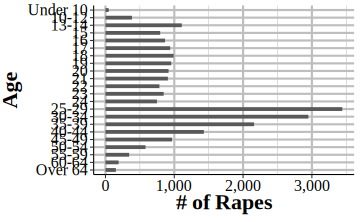
\includegraphics[width=1\linewidth,height=1\textheight]{05_arrests_files/figure-latex/phillyRapeAge-1} 

}

\caption{The total number of rapes by male arrestees reported by arrestee age in Philadelphia, 1974-2022.}\label{fig:phillyRapeAge}
\end{figure}

\subsection{Race}\label{race}

The dataset categorizes arrests by race: American Indian,
Asian, Black, and White. It does not account for mixed-race
individuals or provide details on how race was determined
(e.g., officer perception or arrestee self-reporting). This
is further broken down into if the arrestee was an adult (18
years or older) or a juvenile (under 18).

Whether the arrestee is Hispanic is in a separate (and
nearly universally non-reported variable). Since the
ethnicity variable is separate, and since the data is not at
the arrestee-level unit, there is no way to interact the
race and ethnicity variables. So, for example, there is no
way to determine how many White-Hispanic or
White-Non-Hispanic arrestees. Just total White arrestees and
total Hispanic arrestees.

As with race variables in other UCR datasets - and, really,
any dataset - you should be cautious about using this
variables since it is the officer's perception of the
arrestee's race - though of course some arrests do have
other data about the arrestee's race such as what they tell
the officer. In cases where the arrestee is carrying
identification such as a driver's license this variable is
likely to be extremely well reported. However, we cannot
tell from this data whether the race is based on something
like a license or is merely the officer's
perception.\footnote{In my experience working directly with
  police data where I can identify a person arrested
  multiple times in about 5-10\% of cases they have at least
  one arrest where their reported race is different than
  other arrests. Such as a person arrested five times and
  being reported as White four times and Black once. This is
  probably a mix of officers perceiving people differently
  (e.g.~mixed race people) and having different officers
  report different race for the same person, and human error
  when entering data. But all of it suggests that there is
  at least some uncertainty in this variable.}

Even though there is information about the specific age of
arrestee (or the age range, depending on the arrestee's age)
and their sex, there is no sex information combined with
race and no age beyond the adult/juvenile binary. If you add
up all arrests that are broken down by sex-age and compare
it to the sum of all of the arrests broken down by
adult/juvenile-race here, in some cases these numbers do not
add up. That is because while most agencies do report the
age variables, not all agencies report the race variables.
So summing up the race variables will actually undercount
the total number of arrests.

\begin{itemize}
\tightlist
\item
  American Indian
\item
  Asian
\item
  Black
\item
  White
\end{itemize}

Figure \ref{fig:phillyMarijuanaRacePercent} shows one
example of an analysis of this data by showing the percent
of arrests of adults for marijuana possession by the
arrestee's race in Philadelphia for all years of data we
have with a full year of data reported, 1976-2018 At the
bottom are American Indian and Asian arrestees who make up
nearly none of the arrests for this crime. Black arrestees,
shown in green, make up the bulk of arrests with only a few
years making up under 60\% of arrests and growing to around
80\% of arrests since the mid-2000s. As White arrestees,
shown in orange, are the only other race category included,
they make up a near perfect mirror image of Black arrestees,
composing of around 40\% of arrests until decreasing
starting in the 1990s to end up with about 20\% of arrests
in recent years.

\begin{figure}

{\centering 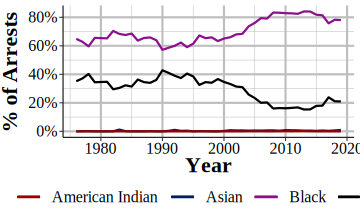
\includegraphics[width=1\linewidth,height=1\textheight]{05_arrests_files/figure-latex/phillyMarijuanaRacePercent-1} 

}

\caption{The annual percent of adult marijuana possession arrests in Philadelphia by arrestee race, 1978-2018.}\label{fig:phillyMarijuanaRacePercent}
\end{figure}

Interestingly, while the disparity between Black-White
arrests has grown dramatically in recent decades, the total
number of arrests have a very different trend as shown in
Figure \ref{fig:phillyMarijuanaRaceCount}. Total marijuana
possession arrests declined in the mid-1980s then increased
in the mid-1990s from only a few hundred arrests in the
early 1990s to nearly 5,000 arrests in 2010 before dropping
precipitously to under 700 each year in the late-2010s.

Yet throughout this latter period as a percent of arrests,
Black people consistently grew for years before plateauing
around 2007 with a small decline in the last few years of
full data. Philadelphia decriminalized marijuana possession
in 2014 under Mayor Nutter which is right when the steepest
decline in arrests happened. This suggests that who is
arrested, in terms of race, is relatively unrelated to the
total number of arrests, at least for marijuana in
Philadelphia.

\begin{figure}

{\centering 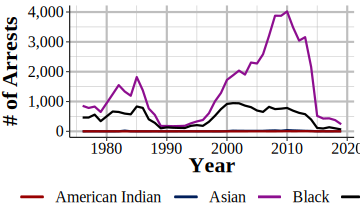
\includegraphics[width=1\linewidth,height=1\textheight]{05_arrests_files/figure-latex/phillyMarijuanaRaceCount-1} 

}

\caption{The annual number of adult marijuana possession arrests in Philadelphia by arrestee race, 1978:2018.}\label{fig:phillyMarijuanaRaceCount}
\end{figure}

\subsection{Ethnicity}\label{ethnicity}

While technically included, the ethnicity variable is
largely useless since for most years no agencies reported it
and for the years where agencies do report ethnicity, not
all agencies do so. The ethnicities included are Hispanic
and non-Hispanic and are broken down by if the arrestee is
an adult (18+ years old) or a juvenile (\textless18 years
old).

\begin{itemize}
\tightlist
\item
  Adult

  \begin{itemize}
  \tightlist
  \item
    Hispanic
  \item
    Non-Hispanic
  \end{itemize}
\item
  Juvenile

  \begin{itemize}
  \tightlist
  \item
    Hispanic
  \item
    Non-Hispanic
  \end{itemize}
\end{itemize}

Figure \ref{fig:theftHispanic} shows the annual number of
Hispanic arrestees for theft for all agencies that reported
any data that year.\footnote{Theft is used as it is one of
  the most common crimes.} For several years no agencies
reported until the number of Hispanic arrestees start
climbing in 1980 and peaks in 1986 at about 136,000
arrestees. Then there are zero Hispanic arrestees for a few
years, four Hispanic arrestees in 1990 and two non-Hispanic
arrests in 1991, and then again zero Hispanic arrestees,
this time for decades. Only in 2017 do the number of
Hispanic theft arrestees begin to creep up. From 2017 to
2022 (the last year available at the time of this writing)
there are Hispanic arrestees reported every year, though now
only about 60,000 per year.

\begin{figure}

{\centering 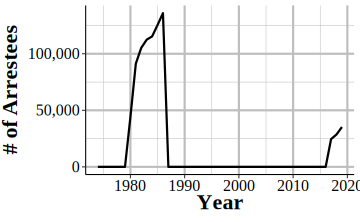
\includegraphics[width=1\linewidth,height=1\textheight]{05_arrests_files/figure-latex/theftHispanic-1} 

}

\caption{The national annual number of Hispanic arrestees for theft. This includes all agencies that year that reporting any number of months. Hispanic arrestees include both juvenile and adult arrestees}\label{fig:theftHispanic}
\end{figure}

Perhaps a better way to look at this data is to see what
percent of agencies report ethnicity data. Figure
\ref{fig:theftHispanicPercentAgencies} show the percent of
agencies each year that report at least one Hispanic or
non-Hispanic (which are the only choices, but showing only
Hispanic arrests would exclude agencies where no Hispanic
people truly were arrested) arrest for theft. About 60\% of
agencies reported ethnicity data in the early 80s and then
only a couple agencies report in 1990 and 1991. Other than
those agencies, none report between 1987 and 2016. Starting
in 2017, 36\% of agencies report and this number has grown
by about five percentage points a year until spiking to
about 67\% in 2021 and it remained steady in 2022. Given the
fluctuations in reporting and how many years there is no
data, I strongly recommend against using these variables,
even for the recent years of data.

\begin{figure}

{\centering 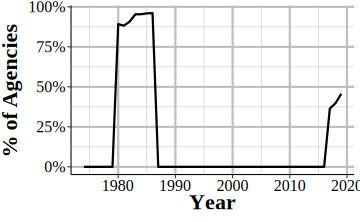
\includegraphics[width=1\linewidth,height=1\textheight]{05_arrests_files/figure-latex/theftHispanicPercentAgencies-1} 

}

\caption{The annual percent of agencies that report theft arrests that reported at least one Hispanic person or one non-Hispanic person arrested for theft. Arrestees include both juvenile and adult arrestees.}\label{fig:theftHispanicPercentAgencies}
\end{figure}

\subsection{Juvenile referrals}\label{juvenile-referrals}

The final variable of interest are five mutually exclusive
outcomes for juveniles who are arrested by the police for a
crime that if they were adults would have been counted as a
formal arrest. This variable is not available for data after
2020.

Unlike the rest of this dataset where juvenile is defined as
being under the age of 18, these variables allow states to
use their own definition of juvenile. So potentially the
limit for who is a juvenile could be below the age of 18,
and nothing in the data indicates when this is so - you
would have to check each state to see their definition and
if it changed over time. There is no breakdown by crime so
this gives you the outcomes for juveniles arrested for all
crimes in that agency. Please note that the number of
juveniles in other variables and the number here do not
always line up, which is a mix of underreporting of this
variable, arrests for other jurisdictions are not counted as
an arrest in the above variables, and different age
definitions for who is a juvenile. A juvenile may
potentially get multiple referrals, such as being released
and then later referred to court. But in this data only the
\emph{initial} referral is included. It is also unclear -
and likely determined by a particular agency's policy - what
is reported when there are multiple initial referrals. Below
are the five potential outcomes and definitions of each:

\begin{itemize}
\tightlist
\item
  Handled within department and released

  \begin{itemize}
  \tightlist
  \item
    Juvenile is arrested but then released without any
    formal charges. Generally released to adult relatives
    with a warning but no formal charge.
  \end{itemize}
\item
  Referred to juvenile court or probation department
\item
  Referred to welfare agency
\item
  Referred to other police agency

  \begin{itemize}
  \tightlist
  \item
    This includes when the agency makes an arrest on behalf
    of a different agency, such as when the juvenile
    committed a crime in that different agency's
    jurisdiction. People arrested in this category are also
    not included in the other variables for juvenile arrests
    (e.g.~arrests by age) as that only includes people who
    committed a crime in the agency's own jurisdiction.
  \end{itemize}
\item
  Referred to criminal or adult court

  \begin{itemize}
  \tightlist
  \item
    These are juveniles who are referred to be tried in
    criminal court as adults. This is for states that allow
    juveniles to be tried as adults. This is the police's
    recommendation that they be tried as adults, regardless
    of the decision of the district attorney or court for
    whether that juvenile is ultimately tried as an adult.
  \end{itemize}
\end{itemize}

We can look at an example of this in Figure
\ref{fig:JuvenileReferrals} which shows the annual number of
referral types in the entire United States from 1974-2022.
For all the first couple of years almost all of the
referrals have either been that the agency handles the
arrest internally and releases the juvenile without any
formal charges, or that the juvenile is formally arrested
and referred to juvenile court. Since this only happens for
a single year it appears to be a data issue.Starting in the
late 1990s the number of referrals has declined over time,
possibly due fewer juvenile arrests overall during this
period.

\begin{figure}

{\centering \includegraphics[width=1\linewidth,height=1\textheight]{05_arrests_files/figure-latex/JuvenileReferrals-1} 

}

\caption{The annual number of juvenile referrals in the United States by referral type, 1974-2020.}\label{fig:JuvenileReferrals}
\end{figure}

In Figure \ref{fig:JuvenileReferrals} there is a massive
spike in referrals to welfare, handled internally, and
juvenile court cases in 1976 that occurs for a single year.
Was this a year of superpredators? No, it was a year of
Michigan data errors. In 1976 many agencies in Michigan
provided erroneous data for this variable. This includes,
for example, Washtenaw County Sheriff's Office which had a
population of 101,452 in 1976 and reported that 150,088
juvenile arrests were reported in welfare. Similarly,
Otisville Police Department, population 760, had 10,000
referrals to welfare, and Saginaw Police Department,
population 82,000, had 80,074 referrals to welfare, 27,213
referrals to juvenile court, and 6,230 juvenile arrests
handled internally. When we remove Michigan, shown in Figure
\ref{fig:JuvenileReferralsNoMichigan}, this spike
disappears.

\begin{figure}

{\centering \includegraphics[width=1\linewidth,height=1\textheight]{05_arrests_files/figure-latex/JuvenileReferralsNoMichigan-1} 

}

\caption{The annual number of juvenile referrals in the United States excluding agencies in Michigan by referral type, 1974-2020.}\label{fig:JuvenileReferralsNoMichigan}
\end{figure}

Michigan is unlikely to be the sole state with data issues
in 1976, and 1976 is unlikely to be the only year with
problems. We can see other spikes in the data such as small
ones in 1991 and 2016. I leave the task of discovering the
cause of these spikes to the reader.

\chapter{Supplementary Homicide Reports (SHR)}\label{shr}

The Supplementary Homicide Reports dataset - often
abbreviated to SHR - is the most detailed of the SRS
datasets and provides information about the circumstances
and participants (victim and offender demographics and
relationship status) for homicides. For each homicide
incident it tells you the age, gender, race, and ethnicity
of each victim and offender as well as the relationship
between the first victim and each of the offenders (but not
the other victims in cases where there are multiple
victims). It also tells you the weapon used by each offender
and the circumstance of the killing, such as a ``lovers
triangle'' or a gang-related murder. As with other SRS data,
it also tells you the agency it occurred in and the month
and year when the crime happened.

One important point of clarification: this is not the number
of murders, though it does track that. This data also
includes the number of homicides that are manslaughter by
negligence (e.g.~children playing with a gun, hunting
accident) and justifiable homicides (i.e.~not criminal). So
be carefully when speaking about this data. It is murders
but not only murders so you want to speak precisely.

\section{Agencies reporting}\label{agencies-reporting-2}

This data only has a report when the agency has a homicide
that year and since homicides are relatively rare it is
difficult to measure underreporting. One way we can look at
reporting is to compare homicide in the SHR data with that
of other datasets. We will look at two of them: the Offenses
Known and Clearances by Arrest which is covered in detail in
Chapter \ref{offensesKnown}, and the Center for Disease
Control and Prevention (CDC) data on national deaths from
homicide.\footnote{CDC WONDER data is available here:
  \url{https://wonder.cdc.gov/}} Both this dataset and the
Offenses Known and Clearances by Arrest data are SHR
datasets so you may think that the numbers of homicides from
each dataset should be the same. That is a perfectly
reasonable assumption, but since this is SHR data we are
talking about, you would be wrong. Police agencies are free
to report to either, both, or neither dataset so while the
number of homicides are close for each dataset, they are
never equal. CDC WONDER data aggregates mortality data
(among other data) from state death certificates which
reduces the issue of voluntary reporting that we have in SHR
data.

Figure \ref{fig:shrVsOffenses} shows the annual number of
homicide victims (including murders and manslaughters) from
each of these datasets starting in 1976 for the SHR data and
in 1999 for the CDC data.\footnote{1975 is actually the
  first year that the Supplementary Homicide Reports data is
  available but that dataset only has info for a single
  victim and offender - all later years has info for up to
  11 victims and offenders - so 1976 is often used as the
  first year of data}

For the SHR data, in every year the numbers are fairly
similar and the trends are the same over time, but the
number of homicides is never equal. The numbers have
actually gotten worse over time with the difference between
the datasets increasing and the Offenses Known data having
consistently more murders reported than the SHR data since
the late 1990s. Compared to the CDC data, however, both SHR
datasets - and in particular the SHR data - undercount the
number of homicides. While trends are the same, SHR data
reports thousands fewer murders per year than the CDC data,
indicating how much of an issue underreporting is in this
data.

\begin{figure}

{\centering 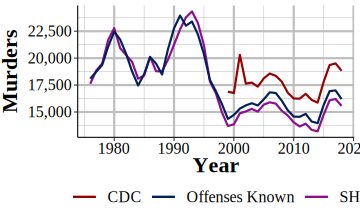
\includegraphics[width=1\linewidth,height=1\textheight]{06_shr_files/figure-latex/shrVsOffenses-1} 

}

\caption{The annual number of murders and nonngeligent manslaughters from the Supplementary Homicide Report and the Offenses Known and Clearances by Arrest dataset, and homicides from the Center for Disease Control (CDC). Numbers differ because agencies voluntarily report and may not report to both datasets.}\label{fig:shrVsOffenses}
\end{figure}

Let us look at Chicago for another example of the
differences in reporting from the SHR and the Offenses Known
data. Figure \ref{fig:chicagoSHRvsOffensesKnown} shows the
annual number of homicide victims from both datasets. In
most years they are pretty similar, excluding a few really
odd years in the 1980s and in 1990. But what is also strange
is that most years have more SHR victims than Offenses Known
victims. So nationally SHR has fewer homicides than Offenses
Known but that pattern is reversed in Chicago? This is one
of the many quirks of SHR data. And is a warning against
treating national trends as local trends; what is true
nationally is not always true in your community. So when you
use this data, check everything closely. And once you have
done that, check it again.

\begin{figure}

{\centering \includegraphics[width=1\linewidth,height=1\textheight]{06_shr_files/figure-latex/chicagoSHRvsOffensesKnown-1} 

}

\caption{The annual number of homicide victims in Chicago, Supplementary Homicide Reports and Offenses Known and Clearances by Arrest, 1976-2022.}\label{fig:chicagoSHRvsOffensesKnown}
\end{figure}

Figures \ref{fig:shrTopAgenciesCount} and
\ref{fig:shrTopAgenciesCountPercent} attempt to get at this
question by looking the number and percent of all incidents
that the top 100, 50 and 10 agencies based on number of
homicide incidents make up out of all homicide incidents in
each year. These agencies are massively disproportionate in
how many homicides they represent - though they are also
generally the largest cities in the country so are a small
number of agencies but a large share of this nation's
population. On average, the 10 agencies with the most
homicide incidents each year - which may change every year -
have over 4,000 homicide incidents and make up about 1/4 of
all homicide incidents reported nationally. The top 50 have
about 7,500 incidents a year, accounting for 46\% of
incidents. The top 100 agencies have a bit under 10,000
incidents a year and make up over 55\% of all homicide
incidents in the United States. So excluding the largest
agencies in the country would certainly undercount
homicides.

\begin{figure}

{\centering \includegraphics[width=1\linewidth,height=1\textheight]{06_shr_files/figure-latex/shrTopAgenciesCount-1} 

}

\caption{The annual number of homicide incidents, showing all agencies, the top 100 agencies (by number of homicide incidents), top 50, and top 10 agencies, 1976-2022.}\label{fig:shrTopAgenciesCount}
\end{figure}

\begin{figure}

{\centering \includegraphics[width=1\linewidth,height=1\textheight]{06_shr_files/figure-latex/shrTopAgenciesCountPercent-1} 

}

\caption{The annual percent of homicide incidents by the top 100 agencies (by number of homicide incidents), top 50, and top 10 agencies, 1976-2022.}\label{fig:shrTopAgenciesCountPercent}
\end{figure}

\section{Important variables}\label{important-variables-3}

The data has demographic information for up to 11 victims
and 11 offenders, as well as the information on the weapon
used by each offender, the relationship between the first
victim and each offender, and the circumstance of the
homicide. The data also has the traditional SHR set of
variables about the agency: their ORI code, population,
state, region and the month and year of this data. One key
variable that is missing is the outcome of the homicide:
there is no information on whether any of the offenders were
arrested.

While there is information on up to 11 victims and
offenders, in most cases, there is only a single victim and
a single offender in each incident. We can use the
additional\_victim\_count and additional\_offender\_count
columns to see how many additional victims/offenders there
are. An additional victim/offender means in addition to the
first one. Even though we have columns for up to 11 victims
and offenders, in very rare instances the
additional\_{[}victim/offender{]}\_count columns may say
there are more than 11 victims/offenders.

To see how the breakdown for the number of victims in each
incident looks, Figure \ref{fig:numberSHRVictims} shows the
percent of incidents with each possible number of
victims.\footnote{There are five incident where there are
  more than 11 victims. For simplicity of the graph, these
  incident are excluded.} In nearly all incidents - 96.0\% -
there was only a single victim. This drops to 3.3\% of
incidents for two victims, 0.5\% for three victims, and only
about 0.2\% of incidents have four or more victims.

\begin{figure}

{\centering 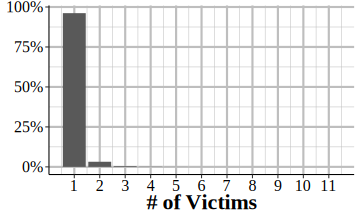
\includegraphics[width=1\linewidth,height=1\textheight]{06_shr_files/figure-latex/numberSHRVictims-1} 

}

\caption{The percent of incidents that have 1-11 victims.}\label{fig:numberSHRVictims}
\end{figure}

Figure \ref{fig:numberSHROffenders} shows the breakdown of
the number of offenders per homicide incident.\footnote{There
  are seven incidents with more than 11 offenders. For
  simplicity of the graph, these incidents are excluded.} It
is a little less concentrated than with victims but the vast
majority of homicides are committed by one offender - or at
least the police only report one offender. About 87.6\% of
homicides have only one offender, 8.4\% have two, 2.5\% have
three, and 1.5\% have four. Fewer than 0.5\% of homicides
have more than four offenders. However, this is all a bit
misleading. In cases where there is no information about the
offender, including how many offenders there is, the data
simply says that there is a single offender. So the number
of homicides with a single offender is an over-count while
the number with more offenders is an undercount.

\begin{figure}

{\centering 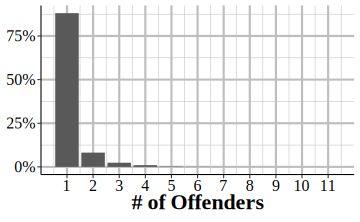
\includegraphics[width=1\linewidth,height=1\textheight]{06_shr_files/figure-latex/numberSHROffenders-1} 

}

\caption{The percent of incidents that have 1-11 offenders.}\label{fig:numberSHROffenders}
\end{figure}

The variable ``situation'' says what type of victim-offender
number combination the incident is - e.g.~``multiple
victims/single offender'', ``single victim/multiple
offenders'', etc. - and does indicate if the number of
offenders is unknown (though curiously there are over 4,000
instances where the number of offenders is unknown but they
still say there are two offenders) so you can use this
variable to determine if the police do not know how many
offenders there is. You're still limited, of course, in that
the number of offenders is always what the police think
there are, and they may be wrong. So use this variable - and
anything that comes from it like the percent of offenders of
a certain race - with caution.

We will now look at a number of important variables
individually. Since the data can potentially have 11 victims
and 11 offenders - but in practice has only one each in the
vast majority of cases - we will only look at the first
victim/offender for each of these variables. Therefore, the
results will not be entirely accurate, but will still give
you a good overview of the data. The figures below will use
data for all homicides from 1976 to 2022 so will cover all
currently available years of data. Keep in mind that
national trends are not the same as local trends so what is
shown in these figures will probably not be the same as what
is happening in your community. And that looking at all
homicides means we are including murders, manslaughters, and
justifiable homicides.

\subsection{Demographics}\label{demographics}

There are two broad categories of variables that we will
cover: demographics of the victim and offenders, and
characteristics of the case. We start with demographics.

\subsubsection{Age}\label{age-1}

This data includes the age (in years) for each victim and
each offender. For those under one years old, it also breaks
this down into those from birth to six days old ``including
abandoned infant'' and those seven days old to 364 days old.
So there is a bit more info on homicides of babies. It also
maxes out the age at 99 so for victims or offenders older
than that we do not get their exact age, just text that says
``99 years or older'' (which I turn to the number 99 in the
figures below).

Figure \ref{fig:shrOffenderAge} shows the percent of
homicides where the first offender in the case is of each
age from 0-99. Offenders with unknown ages are excluded from
this graph and make up about 27\% of cases. The average
(mean) age is 31.1 years old (shown in orange) which is due
to a long right tail; the median age is 28 years old. If you
look closely at the left side of the graph you can see that
there are some very young offenders, with at least one
offender for each year of age from 0 to 10 included in the
data. It is not clear from this alone that these ages are a
data entry error. While a two-year-old certainly could not
kill someone, the data does include deaths caused by
``children playing with gun'' (homicide circumstances will
be discussed in Section \ref{circumstance}) so these ages
could potentially be correct.

If you are familiar with the age-crime curve in criminology
- which basically says crime peaks in late teen years then
falls dramatically - this shows that exact curve, though is
older and does not decline as the offender ages as quickly
as we see with less serious crimes.

\begin{figure}

{\centering 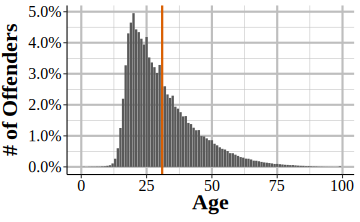
\includegraphics[width=1\linewidth,height=1\textheight]{06_shr_files/figure-latex/shrOffenderAge-1} 

}

\caption{The age of homicide offenders, based on the first offender in any homicide incident. Offenders under age 1 (classified as 'birth to 7 days old, including abandoned infant' and '7 days to 364 days old') and considered 0 years old. Offenders reported as '99 years or older' are considered 99 years old.}\label{fig:shrOffenderAge}
\end{figure}

Figure \ref{fig:shrVictimAge} repeats Figure
\ref{fig:shrOffenderAge} but with victim age rather than
offender age. The mean victim age (shown in orange) is 33
and the median age is 30. Though the average victim age is a
bit younger than the average offender age, trends are
relatively similar for teenagers and older where deaths
spikes in the late teen years and then declines steadily.
The major difference is the U-shape for younger victims -
for victims under age 15, homicides peak at age 0
(i.e.~younger than their first birthday) with
\textasciitilde1.4\% of all homicides being this this age.
They then decline until plateauing at around age 6 before
increasing again in the early teen years.

\begin{figure}

{\centering \includegraphics[width=1\linewidth,height=1\textheight]{06_shr_files/figure-latex/shrVictimAge-1} 

}

\caption{The age of homicide victims, based on the first victims in any homicide incident. Victims under age 1 (classified as 'birth to 7 days old, including abandoned infant' and '7 days to 364 days old') and considered 0 years old. Victims reported as '99 years or older' are considered 99 years old.}\label{fig:shrVictimAge}
\end{figure}

\subsubsection{Sex}\label{sex}

We will next look at victim and offender sex, a simple
variable since only male and female are included. About
62.2\% of offenders, as seen in Figure
\ref{fig:shrOffenderSex}, are male and about 8.2\% are
female, indicating a large disparity in the sex of homicide
offenders. The remaining 29.6\% of offenders do not have sex
data available because the police do not know the sex of
this individual. For offenders who are not arrested, this
variable may be inaccurate since it is perceived sex of the
offender.\footnote{If we ignore unknown sex, essentially
  saying that the unknown people will have their sex
  distributed exactly as the known sex people, 88\% are male
  and 12\% are female. However, this assumption is probably
  wrong since the unknown people may be materially different
  than the known people, as evidence by them likely not
  being arrested and committing the crime in a way where
  even their sex cannot be identified.}

\begin{figure}

{\centering \includegraphics[width=1\linewidth,height=1\textheight]{06_shr_files/figure-latex/shrOffenderSex-1} 

}

\caption{The sex of offender \#1, 1976-2022.}\label{fig:shrOffenderSex}
\end{figure}

There is far less uncertainty for victim sex, with under
0.17\% of victims having an unknown sex. Here again there is
a large disparity between male and female with about 78.2\%
of victims being male and 21.6\% being female.

\begin{figure}

{\centering \includegraphics[width=1\linewidth,height=1\textheight]{06_shr_files/figure-latex/shrVictimSex-1} 

}

\caption{The sex of victim \#1, 1976-2022.}\label{fig:shrVictimSex}
\end{figure}

\subsubsection{Race}\label{race-1}

This data also includes the race of the victims and
offenders. This includes the following races: American
Indian or Alaskan Native, Asian, Black, Native Hawaiian or
Other Pacific Islander, and White. These are the only races
included in the data; Hispanic is considered an ethnicity
and is available as a separate, though flawed, variable.
There is no category for bi- or multi-racial. As with other
demographics info for offenders, in cases where no arrest is
made (and we do not know in this data if one is made), there
is no way to confirm the person's race so these results may
not be entirely accurate.

Figure \ref{fig:shrOffenderRace} shows the percent of
homicides in the data by the race of offender \#1. Black and
White offenders are included are similar percentages, at
34.3\% and 33.6\% of victims, respectively. The next most
common group is Unknown at about 30.6\% of offenders. Given
that so many offenders have an unknown race, the reliability
of race measures is limited. The remaining races are Asian
at 0.9\% of offenders, American Indian or Alaskan Native at
0.6\%, and Native Hawaiian or Other Pacific Islander at
0.02\%.

\begin{figure}

{\centering \includegraphics[width=1\linewidth,height=1\textheight]{06_shr_files/figure-latex/shrOffenderRace-1} 

}

\caption{The race of offender \#1, 1976-2022.}\label{fig:shrOffenderRace}
\end{figure}

For victim race, seen in Figure \ref{fig:shrVictimRace},
only about 1\% of victim \#1 races are unknown. This means
we can be a lot more confident in the race of the victims
than in the race of the offender. Similar to offenders,
White and Black victims are the two most common races, with
48.4\% and 48.1\% of victims, respectively. There is a
greater share of Asian victims than Asian offenders at 1.5\%
of victims. American Indian or Alaskan Natives make up 0.8\%
of victims while Native Hawaiian or Pacific Islanders make
up 0.02\% of victims.

\begin{figure}

{\centering \includegraphics[width=1\linewidth,height=1\textheight]{06_shr_files/figure-latex/shrVictimRace-1} 

}

\caption{The race of victim \#1, 1976-2022}\label{fig:shrVictimRace}
\end{figure}

\subsubsection{Ethnicity}\label{ethnicity-1}

The final demographic variable is ethnicity which is whether
the victim or offender is Hispanic or not Hispanic. The SHR
data has a weird relationship with this variable (which is
also in the Arrests by Age, Sex, and Race dataset, discussed
in Chapter \ref{arrests}) where ethnicity is technically a
variable in the data but very rarely collected. As such,
this is an unreliable variable that if you really want to
use needs careful attention to make sure it is being
reported consistently by the agencies that you are looking
at.

The vast majority - 69.7\% - of offenders have an unknown
ethnicity while 23.4\% are not Hispanic and 7.1\% are
Hispanic.

\begin{figure}

{\centering \includegraphics[width=1\linewidth,height=1\textheight]{06_shr_files/figure-latex/shrOffenderEthnicity-1} 

}

\caption{The ethnicity of offender \#1, 1976-2022.}\label{fig:shrOffenderEthnicity}
\end{figure}

Unlike the other demographic variables, there is still a
huge amount of underreporting when it comes to victim
ethnicity, though still less than for offender ethnicity.
55.6\% of victims have an unknown ethnicity. Approximately
33.2\% of victim \#1 are reported as not Hispanic while
11.1\% are reported as Hispanic.

\begin{figure}

{\centering \includegraphics[width=1\linewidth,height=1\textheight]{06_shr_files/figure-latex/shrVictimEthnicity-1} 

}

\caption{The ethnicity of victim \#1, 1976-2022.}\label{fig:shrVictimEthnicity}
\end{figure}

As an example of agencies under-reporting this variable, let
us look at the number of offender \#1s in Albuquerque, New
Mexico, a city which the
\href{https://www.census.gov/quickfacts/fact/table/albuquerquecitynewmexico,US/PST045222}{US
Census} says is about 50\% Hispanic. Yet the Albuquerque
police reported no ethnicity information for almost three
decades of data.

\begin{figure}

{\centering \includegraphics[width=1\linewidth,height=1\textheight]{06_shr_files/figure-latex/ABQ-1} 

}

\caption{Annual number of offender \#1 who is Hispanic in Albuquerque, New Mexico, 1976-2022.}\label{fig:ABQ}
\end{figure}

\subsection{Case
characteristics}\label{case-characteristics}

Now we will move to facts about each case such as what
weapon was used, how people involved knew each other, and
what was the (rough) cause of the homicide.

\subsubsection{Weapon used}\label{weapon-used}

The first variable we will look at is the weapon used by
each offender. Table \ref{tab:shrWeapon} shows the weapon
used by the first offender in every incident from 1976 to
2022. Each offender can only be reported as having a single
weapon, so this table essentially shows the number (and
percent) of homicides caused by this weapon. This is not
entirely true since in reality an offender could use
multiple weapons and there can be multiple offenders. In
these cases the police include what they believe is the
``primary'' weapon used by this offender.

The most commonly used weapon is a handgun, which is used in
nearly half of homicides. This is followed by a knife or
other sharp weapon used to cut at almost 15\% of homicides,
and then by ``firearm, type not stated'' which is just a
firearm where we do not know the exact type (it can include
handguns) at 8.9\% of homicides The fourth most common
weapon is ``personal weapons'' at nearly 6\% of homicides.
``Personal weapons'' is a weird term to mean that there was
no weapon - the ``weapon'' was the offender who beat the
victim to death. Shotguns are involved in almost 5\% of
homicides and all other weapons are involved in fewer than
5\% of cases. In total there are 19 different weapons
included though most are very uncommon.

\begin{longtable}[t]{l|l|r}
\caption{\label{tab:shrWeapon}The weapon used in a homicide incident, 1976-2022. In cases where there are multiple offenders, shows only the primary weapon for the first offender.}\\
\hline
Weapon & \# of Incidents & \% of Incidents\\
\hline
\endfirsthead
\caption[]{\label{tab:shrWeapon}The weapon used in a homicide incident, 1976-2022. In cases where there are multiple offenders, shows only the primary weapon for the first offender. \textit{(continued)}}\\
\hline
Weapon & \# of Incidents & \% of Incidents\\
\hline
\endhead
Handgun & 388,178 & 49.06\textbackslash{}\%\\
\hline
Knife Or Cutting Instrument & 115,540 & 14.60\textbackslash{}\%\\
\hline
Firearm, Type Not Stated & 70,632 & 8.93\textbackslash{}\%\\
\hline
Personal Weapons - Includes Beating & 45,473 & 5.75\textbackslash{}\%\\
\hline
Other Or Unknown Weapon & 42,002 & 5.31\textbackslash{}\%\\
\hline
Shotgun & 36,827 & 4.65\textbackslash{}\%\\
\hline
Blunt Object & 34,716 & 4.39\textbackslash{}\%\\
\hline
Rifle & 28,108 & 3.55\textbackslash{}\%\\
\hline
Strangulation - Includes Hanging & 9,763 & 1.23\textbackslash{}\%\\
\hline
Fire & 5,380 & 0.68\textbackslash{}\%\\
\hline
Asphyxiation - Includes Death By Gas & 4,804 & 0.61\textbackslash{}\%\\
\hline
Other Gun & 3,473 & 0.44\textbackslash{}\%\\
\hline
Narcotics/Drugs - Includes Sleeping Pills & 3,144 & 0.40\textbackslash{}\%\\
\hline
Drowning & 1,387 & 0.18\textbackslash{}\%\\
\hline
Other Or Type Unknown & 586 & 0.07\textbackslash{}\%\\
\hline
Poison - Does Not Include Gas & 531 & 0.07\textbackslash{}\%\\
\hline
Explosives & 386 & 0.05\textbackslash{}\%\\
\hline
Pushed Or Thrown Out of Window & 257 & 0.03\textbackslash{}\%\\
\hline
Narcotics Or Drugs & 48 & 0.01\textbackslash{}\%\\
\hline
Total & 791,235 & 100\textbackslash{}\%\\
\hline
\end{longtable}

You may have noticed from the table that AR-15 is not
included. While AR-15 is the commonly discussed in the media
and policy circles as a way to control gun violence, it is
not in a category by itself. Instead it is combined with
other rifles in the ``rifle'' weapon group, and makes up
about 3.6\% of the weapons used by offender \#1 in the data.

Let us check if AR-15s, through our rough proxy of the
``rifle'' weapon group, is getting more common over time.
Figure \ref{fig:shrRifle} shows the number of homicide
incidents (including manslaughters, so not necessarily all
murders) where offender \#1 used a rifle. Figure
\ref{fig:shrRiflePercent} shows the percent of all homicide
incidents where the the weapon was a rifle. Using both of
these measures we can see the rifles are getting less
common, declining substantially since 1980 though increasing
again starting in the mid-2010s.

\begin{figure}

{\centering \includegraphics[width=1\linewidth,height=1\textheight]{06_shr_files/figure-latex/shrRifle-1} 

}

\caption{The annual number of homicide incidents where offender \#1's weapon was a rifle, 1976-2022.}\label{fig:shrRifle}
\end{figure}

\begin{figure}

{\centering \includegraphics[width=1\linewidth,height=1\textheight]{06_shr_files/figure-latex/shrRiflePercent-1} 

}

\caption{The annual share of homicide incidents where offender \#1's weapon was a rifle, 1976-2022.}\label{fig:shrRiflePercent}
\end{figure}

Now, maybe this weapon is more commonly used in some types
of crimes such as school shootings. You could get at that
question using this data by seeing if times when a rifle is
used that victims or offenders are younger or if the
circumstance is something that suggests a school shooting.
Unfortunately there is no offense location variable here,
though there is in NIBRS and we can largely recreate this
data through NIBRS. And of course you cannot tell if the
weapon is actually an AR-15, only if it is a rifle.

\subsubsection{Relationship between first victim and
offenders}\label{relationship-between-first-victim-and-offenders}

An interesting and highly useful variable is the
relationship between the first victim and each offender. To
be clear, this is only for the first victim; we do not have
the relationship between other victims and offenders.
However, as seen earlier, this is not \emph{too much} of an
issue since nearly all incidents only have a single victim.
There are 29 possible relationship types (including
``unknown'' relationship) which are broken into three
categories: legal family members, people known to the victim
but who are not family, and people not known to the victim.
Table \ref{tab:shrRelationship} shows these relationships
and the number and percent of homicides with these
relationships.

The most common relationship, with about 28\% of homicides,
is that the police do not know the relationship. So there is
a good deal of uncertainty in the relationship between
victims and offenders. Next is that the victim is the
offender's acquaintance at 19.7\% or is a stranger at
15.3\%. The next is ``other - known to victim'' which is
similar to being an acquaintance at almost 5\% of homicides.
This is followed by the victim being the friend of the
murderer at 3.6\%. The 6th most common relationship, at
3.6\% is that the victim is the wife of the offender, so she
is murdered by her husband, and is the first familial
relationship of this list. The remaining relationships all
make up fewer than 3\% of all homicides.

\begin{longtable}[t]{l|l|r|r}
\caption{\label{tab:shrRelationship}The relationship between the first victim and the first offender in a homicide incident, 1976-2022.}\\
\hline
Relationship & Category & \# of Incidents & \% of Incidents\\
\hline
\endfirsthead
\caption[]{\label{tab:shrRelationship}The relationship between the first victim and the first offender in a homicide incident, 1976-2022. \textit{(continued)}}\\
\hline
Relationship & Category & \# of Incidents & \% of Incidents\\
\hline
\endhead
Unknown &  & 296,757 & 37.51\textbackslash{}\%\\
\hline
Acquaintance & Not family (but known) & 156,115 & 19.73\textbackslash{}\%\\
\hline
Stranger & Not known & 120,719 & 15.26\textbackslash{}\%\\
\hline
Other - Known To Victim & Not family (but known) & 37,899 & 4.79\textbackslash{}\%\\
\hline
Friend & Not family (but known) & 28,411 & 3.59\textbackslash{}\%\\
\hline
Wife & Family & 27,977 & 3.54\textbackslash{}\%\\
\hline
Girlfriend & Not family (but known) & 21,447 & 2.71\textbackslash{}\%\\
\hline
Husband & Family & 12,085 & 1.53\textbackslash{}\%\\
\hline
Other Family & Family & 11,760 & 1.49\textbackslash{}\%\\
\hline
Son & Family & 11,408 & 1.44\textbackslash{}\%\\
\hline
Boyfriend & Not family (but known) & 10,009 & 1.26\textbackslash{}\%\\
\hline
Neighbor & Not family (but known) & 8,081 & 1.02\textbackslash{}\%\\
\hline
Daughter & Family & 8,056 & 1.02\textbackslash{}\%\\
\hline
Brother & Family & 6,961 & 0.88\textbackslash{}\%\\
\hline
Father & Family & 5,667 & 0.72\textbackslash{}\%\\
\hline
Mother & Family & 5,274 & 0.67\textbackslash{}\%\\
\hline
In-Law & Family & 4,608 & 0.58\textbackslash{}\%\\
\hline
Common-Law Wife & Family & 3,317 & 0.42\textbackslash{}\%\\
\hline
Common-Law Husband & Family & 2,722 & 0.34\textbackslash{}\%\\
\hline
Ex-Wife & Not family (but known) & 2,365 & 0.30\textbackslash{}\%\\
\hline
Stepfather & Family & 1,864 & 0.24\textbackslash{}\%\\
\hline
Homosexual Relationship & Not family (but known) & 1,704 & 0.22\textbackslash{}\%\\
\hline
Sister & Family & 1,536 & 0.19\textbackslash{}\%\\
\hline
Stepson & Family & 1,500 & 0.19\textbackslash{}\%\\
\hline
Ex-Husband & Not family (but known) & 937 & 0.12\textbackslash{}\%\\
\hline
Stepdaughter & Family & 792 & 0.10\textbackslash{}\%\\
\hline
Employer & Not family (but known) & 564 & 0.07\textbackslash{}\%\\
\hline
Employee & Not family (but known) & 451 & 0.06\textbackslash{}\%\\
\hline
Stepmother & Family & 250 & 0.03\textbackslash{}\%\\
\hline
Total &  & 791,236 & 100\textbackslash{}\%\\
\hline
\end{longtable}

\subsubsection{Homicide circumstance}\label{circumstance}

We also have information on the type of the homicide, which
this data calls the ``circumstance.'' This comes as
relatively broad categories that leave a lot to be desired
in our understanding of what led to the homicide. Table
\ref{tab:shrCircumstance} shows the number and percent of
each circumstance for the first victim of each homicide from
1976 to 2022. This data has 33 possible circumstances which
it groups into four main categories: murders that coincide
with committing another crime (``felony type'' murders),
murders that do not coincide with another crime
(``non-felony type'' murders), justifiable homicides, and
negligent manslaughter.

The felony type murders are simply ones where another crime
occurred during the homicide. While this is called ``felony
type'' it does include other crimes such as theft and
gambling (which are not always a felony) so is a bit of a
misnomer. The ``non-felony type'' are murders that happen
without another crime. This includes gang killings (where,
supposedly, only the murder occurred), children killed by
babysitters, fights among intoxicated (both of alcohol and
drugs) people, and ``lover's triangle'' killings.
Justifiable homicides are when a person (civilian or police
officer) kill a person who is committing a crime. Negligent
manslaughter includes accidental shootings such as when
children find and shoot a gun, but excludes deaths from
traffic accidents.

The most common circumstances, accounting for 27.4\%,
26.9\%, and 12.5\%, respectively, are ``Unknown'', ``Other
Arguments'', and ``Other Non-Felony Type - Not Specified.''
Since the data includes ``Argument Over Money Or Property''
as one category, the ``Other Arguments'' mean that it is an
argument for a reason other than over money or property. The
``Other Non-Felony Type'' one does not mean that the murder
did not occur alongside another crime, but also does not
fall into the non-felony categories included. Robbery is the
only remaining circumstance with more than 5\% of murders,
at 7.4\%.

\begin{longtable}[t]{l|l|r|r}
\caption{\label{tab:shrCircumstance}The circumstance of the homicide for the first offender in a homicide incident.}\\
\hline
Circumstance & Category & \# of Incidents & \% of Incidents\\
\hline
\endfirsthead
\caption[]{\label{tab:shrCircumstance}The circumstance of the homicide for the first offender in a homicide incident. \textit{(continued)}}\\
\hline
Circumstance & Category & \# of Incidents & \% of Incidents\\
\hline
\endhead
Unknown &  & 219,450 & 27.74\textbackslash{}\%\\
\hline
Other Arguments & Non-Felony Type & 212,941 & 26.91\textbackslash{}\%\\
\hline
Other Non-Felony Type - Not Specified & Non-Felony Type & 98,730 & 12.48\textbackslash{}\%\\
\hline
Robbery & Felony Type & 58,885 & 7.44\textbackslash{}\%\\
\hline
Narcotic Drug Laws & Felony Type & 28,360 & 3.58\textbackslash{}\%\\
\hline
Juvenile Gang Killings & Non-Felony Type & 24,309 & 3.07\textbackslash{}\%\\
\hline
Felon Killed By Police & Justifiable Homicide & 17,553 & 2.22\textbackslash{}\%\\
\hline
Other Felony Type - Not Specified & Felony Type & 15,460 & 1.95\textbackslash{}\%\\
\hline
Brawl Due To Influence of Alcohol & Non-Felony Type & 15,227 & 1.92\textbackslash{}\%\\
\hline
Argument Over Money Or Property & Non-Felony Type & 14,972 & 1.89\textbackslash{}\%\\
\hline
Felon Killed By Private Citizen & Justifiable Homicide & 13,928 & 1.76\textbackslash{}\%\\
\hline
All Suspected Felony Type & Felony Type & 12,975 & 1.64\textbackslash{}\%\\
\hline
All Other Manslaughter By Negligence Except Traffic Deaths & Negligent Manslaughter & 8,536 & 1.08\textbackslash{}\%\\
\hline
Domestic Violence (Historically Called Lovers Triangle/Quarrel) &  & 6,431 & 0.81\textbackslash{}\%\\
\hline
Burglary & Felony Type & 6,356 & 0.80\textbackslash{}\%\\
\hline
Gangland Killings & Non-Felony Type & 5,809 & 0.73\textbackslash{}\%\\
\hline
Brawl Due To Influence of Narcotics & Non-Felony Type & 4,750 & 0.60\textbackslash{}\%\\
\hline
Lovers Triangle & Non-Felony Type & 4,158 & 0.53\textbackslash{}\%\\
\hline
Rape & Felony Type & 4,142 & 0.52\textbackslash{}\%\\
\hline
Other Negligent Handling of Gun Which Resulted In Death of Another & Negligent Manslaughter & 3,877 & 0.49\textbackslash{}\%\\
\hline
Arson & Felony Type & 3,304 & 0.42\textbackslash{}\%\\
\hline
Motor Vehicle Theft & Felony Type & 1,468 & 0.19\textbackslash{}\%\\
\hline
Children Playing With Gun & Negligent Manslaughter & 1,453 & 0.18\textbackslash{}\%\\
\hline
Other Sex Offenses & Felony Type & 1,433 & 0.18\textbackslash{}\%\\
\hline
Child Killed By Babysitter & Non-Felony Type & 1,342 & 0.17\textbackslash{}\%\\
\hline
Institutional Killings & Non-Felony Type & 1,262 & 0.16\textbackslash{}\%\\
\hline
Gambling & Felony Type & 1,040 & 0.13\textbackslash{}\%\\
\hline
Larceny & Felony Type & 916 & 0.12\textbackslash{}\%\\
\hline
Prostitution And Commercialized Vice & Felony Type & 626 & 0.08\textbackslash{}\%\\
\hline
Other - Not Specified & Felony Type & 554 & 0.07\textbackslash{}\%\\
\hline
Sniper Attack & Non-Felony Type & 480 & 0.06\textbackslash{}\%\\
\hline
Victim Shot In Hunting Accident & Negligent Manslaughter & 350 & 0.04\textbackslash{}\%\\
\hline
Gun Cleaning Death - Other Than Self-Inflicted & Negligent Manslaughter & 144 & 0.02\textbackslash{}\%\\
\hline
Abortion & Felony Type & 14 & 0.00\textbackslash{}\%\\
\hline
Human Trafficking/Commercial Sex Acts &  & 1 & 0.00\textbackslash{}\%\\
\hline
Total &  & 791,236 & 100\textbackslash{}\%\\
\hline
\end{longtable}

\subsubsection{Homicide
subcircumstance}\label{homicide-subcircumstance}

The ``subcircumstance'' just tells you more information
about justifiable homicides. This includes the circumstance
leading up to the ``felon'' - which is how the person killed
is described, though technically they do not need to have
committed a felony - was killed. It includes if this person
attacked an officer (the one who killed them), a different
officer, a civilian, or was committing or fleeing a crime.

This dataset is one source of information on how many people
police kill each year. But it is a large undercount compared
to other sources such as the Washington Post collection, so
is not a very useful source of information on this topic.

\begin{longtable}[t]{l|l|r}
\caption{\label{tab:shrSubCircumstance}The circumstance for the first offender in a homicide incident in cases where the offender is killed. This includes incidents where the only person who dies in the offender.}\\
\hline
Subcircumstance & \# of Incidents & \% of Incidents\\
\hline
\endfirsthead
\caption[]{\label{tab:shrSubCircumstance}The circumstance for the first offender in a homicide incident in cases where the offender is killed. This includes incidents where the only person who dies in the offender. \textit{(continued)}}\\
\hline
Subcircumstance & \# of Incidents & \% of Incidents\\
\hline
\endhead
Felon Killed In Commission of A Crime & 11,026 & 35.02\textbackslash{}\%\\
\hline
Felon Attacked Police Officer & 9,224 & 29.30\textbackslash{}\%\\
\hline
Felon Attacked A Civilian & 5,499 & 17.47\textbackslash{}\%\\
\hline
Not Enough Information To Determine & 2,529 & 8.03\textbackslash{}\%\\
\hline
Felon Resisted Arrest & 1,268 & 4.03\textbackslash{}\%\\
\hline
Felon Attacked Fellow Police Officer & 1,096 & 3.48\textbackslash{}\%\\
\hline
Felon Attempted Flight From A Crime & 840 & 2.67\textbackslash{}\%\\
\hline
Total & 31,482 & 100\textbackslash{}\%\\
\hline
\end{longtable}

\chapter{Law Enforcement Officers Killed and Assaulted
(LEOKA)}\label{leoka}

The Law Enforcement Officers Killed and Assaulted data
(sometimes referred to as the ``Police Employees'' dataset),
often called just by its acronym LEOKA (``LEE-OH-KUH''), has
two main purposes. First, it provides counts of employees
employed by each agency - broken down by if they are
civilian employees or sworn officers, and also broken down
by sex (male and female are the only options). And second,
it measures how many officers were assaulted or killed
(including officers who die accidentally such as in a car
crash) in a given month. The assault data is also broken
down into shift type (e.g.~alone, with a partner, on foot,
in a car, etc.), the offender's weapon, and type of call
they are responding to (e.g.~robbery, disturbance, traffic
stop). The killed data simply says how many officers are
killed feloniously (i.e.~murdered) or died accidentally
(e.g.~car crash) in a given month. The employee information
is at the year-level so you know, for example, how many male
police officers were employed in a given year at an agency,
but do not know any more than that such as if the number
employed changed over the year. This dataset is commonly
used as a measure of police employees and is a generally
reliable measure of how many police are employed by a police
agency. The second part of this data, measuring assaults and
deaths, is more flawed with missing data issues and data
error issues (e.g.~more officers killed than employed in an
agency).

\section{Agencies reporting}\label{agencies-reporting-3}

Figure \ref{fig:leokaAgencies} shows the annual number of
police agencies that reported at least one month that year.
The first year of data available, 1960, has about 8,400
agencies reporting though this quickly drops to a trough of
around 4,800 agencies that last for several years. After
some undulations in the 1970s, reporting agencies steadily
increases to nearly 14,000 agencies in the 1980s and remains
steady until declining to around 12,000 by the late 1990s.
Then reporting again steadily increases through 2020 to
about 16,000 agencies by the end. 2021 has a massive drop in
reporting to only about 5,000 agencies and then slightly
increasing in 2022.\footnote{This returns us to the low
  point of historical collection all the back in the 1960s.}

The decline after 2020 is part of what I have referred to as
the ``death and rebirth'' of the SRS. 2020 was the last year
that the FBI accepted SRS data - though in 2022 they began
accepting SRS submissions again. As noted in previous
chapters, this death and rebirth led to changes in both
which agencies reported and what data was reported. In 2021
when only NIBRS was collected, no SRS agencies could report,
but even once they began to accept SRS data again the damage
was done. Some agencies were transitioning from SRS to NIBRS
so reported neither, while others likely made the decision
to stick to NIBRS only - perhaps caused by their data vendor
no longer supporting SRS data.

\begin{figure}

{\centering \includegraphics[width=1\linewidth,height=1\textheight]{07_leoka_files/figure-latex/leokaAgencies-1} 

}

\caption{The annual number of police agencies that report at least month of data, at least one employee, and at least one assault against an officer, 1960-2022}\label{fig:leokaAgencies}
\end{figure}

Part of the decline we see in Figure \ref{fig:leokaAgencies}
is because starting in 2018 - for reasons I am unsure of -
many more agencies started reporting having zero employees.
In Figure \ref{fig:leokaAgenciesEmployees} we can see the
annual number of agencies that report having at least one
employee (civilian or sworn officer). Compared to Figure
\ref{fig:leokaAgencies} we see more agencies reporting since
the 200s, and an earlier but less steep drop in reporting.

I mentioned that LEOKA has two purposes: employee
information and assaults on officers information. You should
really think about this data as two separate datasets as
agencies can report one, both, or neither part. In practice,
more agencies report data on the number of employees they
have than they do for assaults on officers. In Figure
\ref{fig:leokaAgenciesAssaults} we can see that in most
years of data fewer than 6,000 (out of \textasciitilde18k
agencies in the country) report having at least one officer
assaulted. The year with the most agencies reporting
\textgreater1 assault was 2022 with 6,397 agencies. Most
years average about 5,000 agencies reporting at least one
assault on an officer. Though there is variation over time,
the trend is much more settled than in the previous figures
without any sharp decline in recent years. Assaults on
officers is \emph{relatively} rare, at least considering how
many officer-civilian interactions occur. And many agencies
are small with relatively little crime. So agencies that say
they had zero assaults on officers may in fact truly have
zero assaults. However, there are agencies that likely do
have assaults on officers - such as large, high crime
agencies which report assaults in other years - which report
zero assaults in some months or years. So you will need to
be careful when determining if a zero report is a true zero
rather than an agency submitting incomplete data.

\section{Important variables}\label{important-variables-4}

The important variables can be divided into two sections:
information on people employed by the department, and
information about assaults against officers. The employee
information is a snapshot in time during the year while the
assault information tells you the number of assaults, broken
down several different ways, for each month of the year.
Like other UCR data, there are also variables that provide
information about the agency - ORI codes, population under
jurisdiction - the month and year that the data covers, and
how many months reported data.

\subsection{Number of employees}\label{number-of-employees}

This data includes the number of people employed by the
department with breakdowns by if they are civilian employees
or sworn officers (i.e.~carries a gun and badge and can make
arrests) as well as by gender. The only genders available
are female and male. This is the number of employees as of
Halloween that year so it is a single point in time. Though
this helps us as it is consistent every year, we do not know
exactly when certain officer classes start, which we would
likely see through a jump in employment that year, or if
employment or hiring patterns change over the year.

\begin{itemize}
\tightlist
\item
  Officers
\item
  Civilians
\end{itemize}

One of the claims made around the massive crime spike during
Covid is that it was caused, at least in part, by an exodus
of police officers. Fewer police officers led to more crime.
Luckily, we can easily determine if there were fewer
officers employed starting in 2020. In Figure
\ref{fig:leokaNationalEmployees} we have the total number of
sworn officers and civilian employees in the country from
1960 through 2022. The number of both groups has fairly
steadily increased since 1960 until plateuing around 2010
and then fairly sharply dropping in 2018 before rebounding a
bit in 2022. So the number of employees dropped before 2020,
actually increased a tiny bit in 20202 itself, and increased
in 2022. Obviously all the claims about a declining number
of officers was wrong.

Well, not quite. This country's population has grown quite a
bit since 1960 so we really want to do some kind of rate of
officers per civilian population. And as we saw earlier not
all agencies report data. So changes over time may really
just be changes in which agencies report data. For a good
comparison we need to look at only agencies that have
reported data for every year we are interested in. And that
is all assuming we actually care about national trends which
we really should not. Crime is a local issue; what happens
in your community - be it whether officers are leaving or
crime is increasing - matters a whole lot more than what is
happening across the country.\footnote{Of course what
  happens nationally may be reflected locally, but there is
  no good reason to focus on national data in lieu of local
  data.}

\begin{figure}

{\centering \includegraphics[width=1\linewidth,height=1\textheight]{07_leoka_files/figure-latex/leokaNationalEmployees-1} 

}

\caption{The number of civilian employees and sworn officers in the United States, 1960-2022}\label{fig:leokaNationalEmployees}
\end{figure}

So now lets look at a local example: the Philadelphia Police
Department as shown in Figure
\ref{fig:leokaCivilianOfficers}. The number of civilian
employees has remained at a little under 1,000 employees
from about 1970 through the end of our data, though
declining very slightly since the middle 2000s. This is
curious since the city's population and crime trends have
changed dramatically over this time and the ability of
civilian employees to contribute has also changed, such as
that they now have computers.\footnote{The last time I
  heard, which was several years ago, patrol officers in
  Philadelphia still had to write up certain reports using
  typewriters. So tech apparently is still about 1960 level.}
In contrast, the number of police has changed far more than
civilians, growing rapidly in the 1960s and 1970s to peaking
at a little over 8,000 officers in the mid-1970s before
declining substantially to the 6,000s. in the late-1980s. As
with some larger agencies nationwide, the number of officers
increased in the 1990s and then has decreased steadily in
ensuing years. By recent years there are about as many
officers as in the late-1980s, even though the city's
population has grown substantially since then. What stands
out is that in 2020 there are zero sworn officers or
civilians employees. By 2022 there are fewer sworn officers
but more civilian employees than in 2020. 2021 is simply due
to Philly reporting zero employees in that year, though
obviously this is not actually a reflection of reality. When
looking at only one city like we do here it is glaringly
obvious that there is a data issue. The problem is that when
looking at aggregate data, like we do in Figure
\ref{fig:leokaNationalEmployees} it is much harder, without
additional data cleaning steps, to determine what is a data
error and what is a true change.

\begin{figure}

{\centering \includegraphics[width=1\linewidth,height=1\textheight]{07_leoka_files/figure-latex/leokaCivilianOfficers-1} 

}

\caption{The number of civilian employees and sworn officers in the Philadelphia Police Department, 1960-2022}\label{fig:leokaCivilianOfficers}
\end{figure}

We can also look at the number of officers (or civilian
employees) by gender. Figure \ref{fig:leokaOfficersGender}
shows the percent of Philadelphia police officers by gender
while Figure \ref{fig:leokaOfficersGenderCount} shows the
number of officers. For the first decade of data all female
officers (or civilians) were recorded as male, so that
variable should be interpreted as ``total officers'' until
1971 when it is split into gender. Starting at basically 0\%
of officers in 1971, female officers grew until they made up
about a quarter of officers in 2000 and then has declined
slowly since then.\footnote{Please note that since Philly
  did not report in 2021 the 2021 value is NA, and is shown
  in the figure as the 2020 data point drawing a straight
  line to the 2022 data point.}

\begin{figure}

{\centering \includegraphics[width=1\linewidth,height=1\textheight]{07_leoka_files/figure-latex/leokaOfficersGender-1} 

}

\caption{The percent of female and male sworn officers in Philadelphia, 1960-2022}\label{fig:leokaOfficersGender}
\end{figure}

\subsection{Officers killed}\label{officers-killed}

There is almost no information about officers killed. The
data only breaks this down into if they died ``feloniously''
which just means that someone killed them on purpose
(e.g.~shooting them, intentionally hitting them with a car)
or if they died ``accidentally'' such as if they die during
a car crash while on duty. The FBI actually collects more
information on officer deaths than they release in this
data. This includes the circumstances of each death such as
the type of death (e.g.~car crash, shooting, ambush, etc.),
what weapon the offender had if feloniously killed, and even
a detailed written summary of what occurred for each officer
killed. They post this information in their annual LEOKA
report which is part of their Crime in the United States
report. The 2019 report, for example, can be found on their
site \href{https://ucr.fbi.gov/leoka/2019/home}{here}.

We can look at what data is available through Figure
\ref{fig:leokaOfficersKilled} which shows the number of Los
Angeles Police Department officers killed over time. There
are no accidental killings until 1975 though this is
misleading because that accidental killings variable is not
reported until 1971, which is a year in which many other
variables in this data began reporting. So we actually have
no idea how many officers were killed accidentally from
1960-1970 since this variable is always reported as 0. In
general it seems like there is about one officer killed per
year in recent decades while the period from 1980 to 2000
was the time of highest danger with as many as five officers
killed in a single year. We can also see some trend changes
with felonious killings more common than accidental killings
in the 1990s and then accidental killings becoming far more
common starting in 2000.

\begin{figure}

{\centering \includegraphics[width=1\linewidth,height=1\textheight]{07_leoka_files/figure-latex/leokaOfficersKilled-1} 

}

\caption{The number of officers killed by felony and killed accidentally in New York City, 1960-2022}\label{fig:leokaOfficersKilled}
\end{figure}

We can also look at the national number of officers killed
as shown in Figure \ref{fig:leokaOfficersKilledNational}.
Please note that this is simply summing up the number of
officers killed by all agencies that report that year so
changes over time are certainly partially due to different
agencies reporting each year. Therefore, we will focus on
interpreting the different between felony and accidental
killings rather than counts over time - though even this may
be off if agencies that reported more felony or more
accidental killings differ in their reporting over time.
Again we see that there are no officers killed accidentally,
due to that variable not being reported, until 1971. The
difference between officers killed by felony and killed
accidentally is widest are the start of our data and narrows
considerable until there are only several more felonious
killings than accidental killings by the late 1990s. This
trend reverses in the early 2010s with accidental killings
decreasing and felonious killings increasing again.

The last several years of data have extremely few officers
killed accidentally, with fewer than 10 a year since 2018
and even zero officers killed in 2021. According to the
website
\href{https://www.odmp.org/search/year?year=2021}{Officer
Down Memorial Page}, there were 719 officers who died in
2021, including some that should meet the killed
accidentally criteria.\footnote{The vast majority of
  officers who died in 2021 died from Covid.} For example,
23 officers were reported to have been killed by an
automobile crash. So this data on officers killed is
incorrect, is an undercount, and should be used only with a
great deal of caution.

\begin{figure}

{\centering \includegraphics[width=1\linewidth,height=1\textheight]{07_leoka_files/figure-latex/leokaOfficersKilledNational-1} 

}

\caption{The national number of officers killed by felony and killed accidentally, 1960-2022}\label{fig:leokaOfficersKilledNational}
\end{figure}

\subsection{Assaults by injury and
weapon}\label{assaults-by-injury-and-weapon}

This data breaks down the monthly number of assaults on
officers in a few different ways. Here, we will look at the
number of assaults where the officer is injured or not
injured and within these categories by which weapon the
offender had. This is the number of officers assaulted so if
an incident has three officers assaulted, that will count as
three different assaults. If the offender used multiple
weapons then only the most serious weapon would be counted.
For example, if an offender used a knife and a gun during
the assault, the assault would be counted as a gun assault.
Unfortunately we only know if an officer was injured or not
and not the severity of the injury. So we cannot tell if the
officer is merely bruised or was shot or stabbed.

\begin{itemize}
\tightlist
\item
  Assaults with injury
\item
  Offender has firearm
\item
  Offender had knife
\item
  Offender had other weapon
\item
  Offender was unarmed
\item
  Assaults without injury
\item
  Offender has firearm
\item
  Offender had knife
\item
  Offender had other weapon
\item
  Offender was unarmed
\end{itemize}

We can start by looking at the breakdown of assaults by
injury and weapon type for officers in the Los Angeles
Police Department. Figure \ref{fig:leokaAssaultTypeInjury}
shows the number of assaults from all years reported for
these categories. Over the complete time period there were
almost 43,000 officers assaulted with about three-quarters
of these assaults - 33,000 assaults - leading to no
injuries. This data shows the number of officers assaulted,
not unique officers, so an officer can potentially be
included in the data multiple times if they are assaulted
multiple times over a year. A little under a quarter of
assaults lead to officer injury with most of these from
unarmed offenders. Interestingly, there are far more gun and
knife assaults where the officer is not injured than where
the officer is injured. There are likely cases when the
offender threatens the officer with the weapon but does not
shoot or stab the officer.

\begin{figure}

{\centering \includegraphics[width=1\linewidth,height=1\textheight]{07_leoka_files/figure-latex/leokaAssaultTypeInjury-1} 

}

\caption{The total number of assaults on officers by injury sustained and offender weapon in Los Angeles, 1960-2022.}\label{fig:leokaAssaultTypeInjury}
\end{figure}

We can also look at assaults over time. Figure
\ref{fig:leokaAssaultsInjuryYear} shows the number of
assaults, assaults with injury, and assault without injury
for the Los Angeles Police Department from 1960 to 2018. We
can immediately see some data issues are there are years
with no assaults recorded. And in the late-2000s there is a
sudden drop from about 250 assaults with injuries per year
in the previous few decades to nearly zero officer injuries
reported a year. This strongly suggests some change in
reporting rather than a true decrease in assaults with
injuries. For the decades where the data is less obviously
wrong, there is a consistent trend of most assaults leading
to no injuries, though the distance between the number of
injury and non-injury assaults fluctuates over time.

\begin{figure}

{\centering \includegraphics[width=1\linewidth,height=1\textheight]{07_leoka_files/figure-latex/leokaAssaultsInjuryYear-1} 

}

\caption{The annual number of assaults on officers by injury sustained in New York City, 1960-2022.}\label{fig:leokaAssaultsInjuryYear}
\end{figure}

\subsection{Assaults by call
type}\label{assaults-by-call-type}

The next group of ways that assaults are broken down is by
the type of call the officer is assigned when they are
assaulted. For example, if an officer is responding to a
burglary report, any assault they experience on that call
will be classified as ``burglary'' related. In addition, we
know how many assaults were cleared by arrest or cleared
through exceptional means (for more on this, please see
Section \ref{clearedCrimes}) though it does not
differentiate between the two. Since assaults are based on
the number of officers assaulted, not the number of
incidents where officers are assaulted, arresting a single
person can clear multiple assaults. The possible call types
are below:

\begin{itemize}
\tightlist
\item
  Disturbance call (e.g.~domestic violence, person carrying
  a gun in public)
\item
  Burglary
\item
  Robbery
\item
  Officers arresting someone for another crime
\item
  Civil disorder
\item
  Officer has custody of prisoners
\item
  Suspicious persons
\item
  Officers are ambushed
\item
  Mentally deranged person
\item
  Traffic pursuit and traffic stops
\item
  All other call types
\item
  Total - sum of all call types
\end{itemize}

Figure \ref{fig:leokaAssaultCallType} shows the number of
assaults on Los Angeles Police Department officers by the
type of call for 1960-2022. There were about 41,000 assaults
against Los Angeles Police Department officers with a little
over 33,500 of these assaults cleared. An important thing to
note is that the number of assaults here is less than the
nearly 43,000 assaults for the same agency over the same
time period we saw in Figure
\ref{fig:leokaAssaultTypeInjury}. This is because some
variables are not reported for all years and agencies are
free to report which variables they want to report in any
given year. This makes it massively tricky to use this data
since even simple statistics for the same agency for
supposedly the same variable (here it is technically
different variables but should still be the total number of
officers assaulted) can be different.

The most common type of call where officers are assaulted
are disturbance calls which include domestic violence and
reports of dangerous individuals such as people carrying
guns in public. The least common call type is ambush calls,
though in these calls the police are called to a scene by
the offender who intends to assault or kill the officers, so
is likely far more dangerous than other call types, even
though it is rare.

\begin{figure}

{\centering \includegraphics[width=1\linewidth,height=1\textheight]{07_leoka_files/figure-latex/leokaAssaultCallType-1} 

}

\caption{Assaults on Los Angeles Police Department officers by type of call where they were assaulted at, 1960-2022.}\label{fig:leokaAssaultCallType}
\end{figure}

Within these call types is also a breakdown by offender
weapon use, with the same weapons as above, and the type of
officer assignment which is essentially if they are alone or
not and if they are on foot or not. Finally, it says how
many assaults are cleared by arrest or cleared through
exceptional means, though it does not differentiate between
the two. The shift assignment is essentially how they go
through their normal day, if this is in a vehicle, alone, as
a detective, or under a different assignment (including
being off-duty). For example, being in a vehicle with two
officers means that their normal assignment is driving in a
vehicle, not that they were actually assaulted in said
vehicle. This also does not necessarily mean that these are
the only officers at the scene. It is simply the shift
assignment of the officer who is assaulted. For example, if
an officer who normally works alone in a vehicle shows up to
a scene where other officers are present, and who are under
different shift assignments, and gets assaulted - and no one
else gets assaulted - that is an assault for officers ``in a
vehicle alone''.

\begin{itemize}
\tightlist
\item
  Offender weapons
\item
  Offender has firearm
\item
  Offender had knife
\item
  Offender had other weapon
\item
  Offender was unarmed
\item
  Type of officer shift assignment
\item
  In a vehicle with two officers
\item
  In a vehicle alone
\item
  In a vehicle alone but assisted by other officers
\item
  Detective or special unit alone
\item
  Detective or special unit assisted by other officers
\item
  Other assignment alone
\item
  Other assignment assisted by other officers
\item
  Number of assaults on police cleared
\end{itemize}

We will look specifically at disturbance calls since they
are the most common call type, at least for the Los Angeles
Police Department. Figure \ref{fig:leokaDisturbanceWeapon}
shows the total number of disturbance assaults by offender
weapon in Los Angeles. Most assaults have an unarmed
offender with a sharp decline to the number of offenders
with a weapon other than a gun or knife. Assaults by a gun
and by a knife are the least common.

\begin{figure}

{\centering \includegraphics[width=1\linewidth,height=1\textheight]{07_leoka_files/figure-latex/leokaDisturbanceWeapon-1} 

}

\caption{The number of assaults on Los Angeles Police Department officers in disturbance calls by the injury sustained by the officer, 1960-2022.}\label{fig:leokaDisturbanceWeapon}
\end{figure}

Again using disturbance calls for the Los Angeles Police
Department, we can look at assaults by the officer
assignment, as seen in Figure
\ref{fig:leokaShiftAssignment}. In the vast majority of
assaults it is of officers who are in a vehicle along with a
partner. This drops very sharply to several hundred assaults
on detectives who are assisting other officers and then
increasingly declines to the other shift assignments to the
least common assault being against detectives who are acting
alone. So are officers in two-man vehicles are much higher
risk of assaults than officers alone or of detectives?
Almost certainly not. To determine the risk for officers we
need to know how officers are generally deployed. If the
vast majority of officers are in two-man cars then it makes
sense that the vast majority of assaults are on these
assignments. Like most FBI data - and most crime data in
general - we have the numerator (in this case the number of
assaults by shift assignment type) and do not have a proper
denominator (such as the distribution of shift assignments
for all LAPD officers) to determine a rate of risk. Without
this we can present some descriptive statistics but cannot
be more useful by determining, for example, if officers in
certain shift assignments are at higher risks of being
assaulted.

\begin{figure}

{\centering \includegraphics[width=1\linewidth,height=1\textheight]{07_leoka_files/figure-latex/leokaShiftAssignment-1} 

}

\caption{The number of assaults on Los Angeles Police Department officers in disturbance calls by the injury sustained by the shift assignment of the officer, 1960-2022.}\label{fig:leokaShiftAssignment}
\end{figure}

\subsection{Assaults by time}\label{assaults-by-time}

The final breakdown in assaults is by the time they occur,
divided into 12 two-hour chunks starting at 12:01am. Like
some other variables this data is only available starting in
1971. There is no more information than total assaults in
this time so we do not know if the assaults led to injuries,
the type of call or shift assignment the officer was on, or
the offender's weapons.

\begin{itemize}
\tightlist
\item
  12:01am - 2:00am
\item
  2:01am - 4:00am
\item
  4:01am - 6:00am
\item
  6:01am - 8:00am
\item
  8:01am - 10:00am
\item
  10:01am - 12:00pm
\item
  12:01pm - 2:00pm
\item
  2:01pm - 4:00pm
\item
  4:01pm - 6:00pm
\item
  6:01pm - 8:00pm
\item
  8:01pm - 10:00pm
\item
  10:01pm - 12:00am
\end{itemize}

We will look at these time chunks in Figure
\ref{fig:phoenixAssaultTimes} which shows the total number
of assaults by time of day from 1971 to 2018 in Phoenix,
Arizona. The most common times for officers to be assaulted
looks pretty similar to when crime is highest: late night
and early morning. The 12:01am to 2am chunk is the most
common time followed by 10pm to midnight, with assaults
increasing at the day grows later and at its lowest point
from 6-8am. This strongly suggests that officers are
assaulted at crime scenes, such as responding to crimes or
making arrests.\footnote{In the chapters on NIBRS I will
  argue against placing too much trust about time which
  includes midnight, such as the 12:01am to 2am chunk here,
  because there is evidence that some agencies may use it as
  the default time when the true time is unknown. That
  probably happens here as well. While in nearly every
  officer assault the time should be known, there may still
  be instances where the reported time is unknown, such as
  an officer being assaulted at a certain time but
  forgetting to mark it when entering the report.}

\begin{figure}

{\centering \includegraphics[width=1\linewidth,height=1\textheight]{07_leoka_files/figure-latex/phoenixAssaultTimes-1} 

}

\caption{The number of assaults against Phoenix Police Department officers by hourly grouping for all years with data available, 1971-2018.}\label{fig:phoenixAssaultTimes}
\end{figure}

\chapter{Arson}\label{arsonChapter}

The arson dataset provides monthly counts of reported arson
incidents, with detailed breakdowns by type (e.g., arson of
residential properties, vehicles, or public buildings) and
the estimated value of property damage. The data spans from
1979 to the present and includes additional information on
arrests, clearances, and unfounded cases.

This data includes all arsons reported to the police or
otherwise known to the police such as when an officer
discovers it while on patrol. It also has a count of arsons
that lead to an arrest (of at least one person who committed
the arson) and of reports that turned out to not be arsons,
such as if an investigation found that the fire was started
accidentally. This is essentially the Offenses Known and
Clearances by Arrest data, detailed in Chapter
\ref{offensesKnown}, but for arsons. The data even follows
the same definitions for categories such as what counts as a
cleared or unfounded crime. The primary additional variable
is the estimated damage in dollars caused by the arson. As
much of this information is the same as detailed in Chapter
\ref{offensesKnown}, this chapter will be brief. If you have
a question about definitions, please refer to that chapter.

The dataset includes a variable indicating whether the arson
occurred in an uninhabited structure, which refers to
buildings that are vacant, abandoned, or not in regular use.
This allows for estimates of how many building arsons had
the potential to harm people, distinguishing between, for
example, a vacant warehouse and a home where people could be
harmed.

In cases where the arson led to a death, that death would be
recorded as a murder on the Offenses Known and Clearances by
Arrest dataset - but not indicated anywhere on this dataset.
If an individual who responds to the arson dies because of
it, such as a police officer or a firefighter, this is not
considered a homicide (though the officer death is still
included in the Law Enforcement Officers Killed and
Assaulted data) unless the arsonist intended to cause their
deaths.

\section{Agencies reporting}\label{agencies-reporting-4}

This dataset measures how many months that an agency reports
data over a year in the same way as the Offenses Known data
does: the standard FBI definition using the last month
reported, and my own measure counting how many months
reported data according to a column for each month that says
so.\footnote{This is different than identifying how many
  months have an arson as there may be months that truly do
  not have any arsons. We do not want to count those are
  non-reporting months.} And just like the Offenses Known
data, the variable I use for my own measurement changed in
2018, leading to fewer months of data reported and making it
non-comparable to pre-2018 data. The variable changed again
in 2021 and said that all agencies always reported data in
every month, making the variable useless.

In Figure \ref{fig:arsonAgencies} we can see the annual
number of agencies that reported at least one month of data
using both measures. These measures are nearly identical
every year with the last month reported having slightly more
agencies reported, but they are effectively the same. This
changes in 2018 as my measure declines considerably and then
skyrockets to nearly 25,000 agencies in 2021 and 2022. The
last month reported variable declines considerably in 2021,
consistent with the FBI ending SRS collection, and then
rebounds in 2022 when the FBI reopens SRS collection. How
can there be more than 18k agencies reporting? The 18k
number is the estimated number of agencies that are active:
agencies that can respond to crimes and do investigations.
Remember that SRS data goes back decades - the Offenses
Known data is available since 1930. So agencies can come and
go, with agencies shutting down or joining with other
agencies. Over time this adds up to thousands of agencies
other than the 18k we normal think about.

\begin{figure}

{\centering \includegraphics[width=1\linewidth,height=1\textheight]{08_arson_files/figure-latex/arsonAgencies-1} 

}

\caption{The annual number of police agencies that report at least month of data and all 12 months of data, using both measures of how many months are reported, 1979-2022.}\label{fig:arsonAgencies}
\end{figure}

\section{Important variables}\label{important-variables-5}

Similar to the Offenses Known and Clearances by Arrest data,
this data shows the monthly number of crimes - in this case
only arsons - reported or discovered by the police, the
number found by police to be unfounded, and the number
cleared by the police. In addition, it includes the number
of arsons in structures that were uninhabited, and the
estimated cost of the damage caused by the arsons. For each
variable, the arsons are also broken into several categories
of arsons, which we will talk about in Section
\ref{arsonType}. As with other SRS datasets, there are also
variables that provide information about the agency - ORI
codes, population under jurisdiction - the month and year
that the data covers, and how many months reported data.
When another agency submits data for the given agency, that
is noted in the data through the ``covered\_by\_ori''
variable.

\subsection{Types of arsons}\label{arsonType}

For each of the outcome categories detailed below, this
dataset has information for ten different \emph{types} of
arson. Arsons are categorized into three main groups:
building arsons, vehicle arsons, and other arsons (e.g.,
fires in outdoor areas like parks or forests). Building
arsons are further subdivided into seven types, such as
single-family homes, industrial buildings, and public
structures. For each of the building arsons we also have
variables that say how many of the arsons were of
uninhabited buildings. Vehicle arsons are split between
motor vehicles and other mobile objects, such as boats or
airplanes.

\begin{itemize}
\tightlist
\item
  Total structures (buildings)

  \begin{itemize}
  \tightlist
  \item
    Single occupancy (e.g.~single family homes)
  \item
    Other residential (e.g.~hotel, apartment)
  \item
    Storage (warehouses, storage facilities)
  \item
    Industrial
  \item
    Other commercial (e.g.~restaurant, office building, car
    dealership)
  \item
    Community/public (e.g.~government buildings, hospitals,
    community centers, places of worship)
  \item
    All other structures (all buildings that do not fit in
    another category')
  \end{itemize}
\item
  Total mobile vehicles (vehicles)

  \begin{itemize}
  \tightlist
  \item
    Motor vehicles (a car that runs on a road such as a SUV,
    sedan, motorcycle)
  \item
    Other mobile vehicles (other mobile objects such as
    airplanes and boats)
  \end{itemize}
\item
  Other (everything that does not fit in a previous
  category)
\item
  Grand total (all arsons of any category)
\end{itemize}

Some arsons can burn down multiple types or structures or
cars - fire, after all, tends to spread. This data defines
the arson based on where the fire originated, regardless of
what burns after that. This is true even if the damage is
more severe for a type other than where the fire started.
For example, a
\href{https://www.nbcnews.com/news/us-news/man-pushing-burning-car-ravine-started-park-fire-burning-45000-acres-c-rcna163697}{recent
fire in California} was started by a man ``pushing a burning
car into a ravine.'' That fire, known as the Park Fire has
burned over 429,000 acres and over 700 buildings. This fire
would be classified as a motor vehicle arson because the
fire started in a vehicle.

\subsection{Actual arsons}\label{actual-arsons}

This variable includes the number of arsons either reported
to the police or otherwise known to the police in that month
and that the police determine to actually be arsons - that
is, reports that are not unfounded. This is the number of
arsons, regardless of their severity. An arson that burns
down a single vehicle is treated as one arson, as is an
arson that burns down a vehicle, 429 thousand acres of land,
and 600 buildings.

\subsection{Unfounded arsons}\label{unfounded-arsons}

This variable shows the number of arsons reports that the
police determined to not actually be arsons. For example, if
a house burns down and police think it was arson but later
determine that it was an accident, it would be an unfounded
arson. Whether an arson is unfounded is based only on the
police's determination about that event, not the decision of
other groups like a court or the conviction of someone for
the crime. However, this doesn't mean that the officer makes
that decision in a vacuum as they can use evidence such as
the findings from firefighters for if the fire was an arson.

\subsection{Reported arsons}\label{reported-arsons}

This variable is the sum of actual arsons and unfounded
arsons - it is the total number of arsons that were reported
or known to the police, even if a later investigation found
that it was not actually an arson.

\subsection{Cleared arsons}\label{cleared-arsons}

This shows the number of arsons where at least one offender
is arrested or when an arrest cannot be made for some
reason, but the police know who the offender is - the latter
option is called ``exceptional clearances'' or ``clearances
by exceptional means.'' There is no way to tell if a
clearance is due to an arrest or due to exceptional
means.\footnote{NIBRS data does tell more information about
  the type of arrest, but SRS data does not.}

Please note that this data is at the incident-level which
means that having multiple people arrested for an incident
still only is a clearance for that single incident. If there
are multiple people who committed the arson only one needs
to be arrested or exceptionally cleared for the incident to
be cleared.

Clearances are reported in the month they occur, which may
be different than the month when the arson happened. This
can create the illusion that more crimes are solved than
were reported in certain time periods. Figure
\ref{fig:arsonClearance}, for example, shows the number of
actual arsons (reports that are founded) and clearances for
single-family home arsons in League City, Texas, a city of
about 100,000 outside of Houston. In most years there were
fewer clearances than arsons, but in four years (1982, 1981,
1992, and 2007) there were more clearances than arsons.

\begin{figure}

{\centering \includegraphics[width=1\linewidth,height=1\textheight]{08_arson_files/figure-latex/arsonClearance-1} 

}

\caption{The annual number of single-family home arsons and clearances in League City, Texas, 1979-2022.}\label{fig:arsonClearance}
\end{figure}

\subsection{Cleared for arsons where all offenders are under
age
18}\label{cleared-for-arsons-where-all-offenders-are-under-age-18}

This variable is the same for normal clearances but only for
arsons where every offender is under the age of 18. For
juvenile offenders, a clearance can still occur if the
juvenile is issued a citation to appear in court, even if
they are not formally arrested and taken into custody. As
this variable requires that the police know the identity of
every offender (to be able to determine that they are all
under 18), it is likely flawed and merits caution when
using.

\subsection{Uninhabited building
arsons}\label{uninhabited-building-arsons}

This data also includes the number of arsons that occur in
uninhabited structures. These structures must be uninhabited
in the long-term, not simply having no one inside them when
the arson occurs. In the FBI's manual for this data they
define uninhabited buildings as ones that are ``uninhabited,
abandoned, deserted, or not normally in use'' at the time of
the arson. For example, a vacation home whose owners are not
living in at the time would be ``not normally in use'' so
would be an uninhabited building. A business that is closed
when the fire started, but is open during the day, is not an
uninhabited building.

\subsection{Estimated damage
cost}\label{estimated-damage-cost}

The final variable is the estimated cost of the arson. This
is how much the police estimates the value (in dollars) of
the damaged or destroyed property is. Since this is the
value of property damage, injuries to people (including
non-physical injuries such as trauma or mental health costs)
are not included. Since this is estimated damage it may be
inaccurate to some degree. This variable is the sum of
monthly estimated cost so while you can get the average cost
by dividing this by the number of actual offenses, this
average may be significantly off due to having extremely
small or large values in your data. This value may be \$0
since arsons include attempted arsons which may cause little
or no damage. Please note that this value is not
inflation-adjusted so you will have to adjust the value
yourself.

\section{Data errors}\label{data-errors-1}

As with other SRS datasets, the arson data sometimes
includes clear data entry errors, such as reporting
implausibly high numbers of arsons for small jurisdictions
or recording unrealistic damage estimates. For example,
Figure \ref{fig:residenceArson} shows the annual number of
single-family home arsons in Byron City, Illinois, which has
a population of slightly over 3,600 people. In every year
there are zero arsons reported until 2003 when 469 arsons
are reported. Since it is exceedingly unlikely that suddenly
an eighth of the city each suffered different arson attacks,
and that the city never again had a residence arson, this is
almost certainly a data entry error. As arsons are
relatively rare, having errors - and especially ones like
this - can drastically change the results of your analysis
so it is important to check your data carefully for more
errors.

\begin{figure}

{\centering \includegraphics[width=1\linewidth,height=1\textheight]{08_arson_files/figure-latex/residenceArson-1} 

}

\caption{Annual single-family home arsons in Byron  City, Illinois. The sudden spike to over 400 arsons in a single year is an example of data errors in this dataset, 1979-2022. }\label{fig:residenceArson}
\end{figure}

There are also cases where it is less clear when a value is
a data error or is simply due to an outlier - but real -
value. For example, Figure \ref{fig:arsonCost} shows the
annual average cost of a single-family home fire in Los
Angeles, California. In most years the value is low. Since
an arson can cause little or no damage, these low values
likely mean that on average only part of the house was
damaged, rather than the entire house burning down. In 2009,
however, the average damage is about \$540,000 per arson. Is
this a data entry error that simply inputs a damage value
that is too high? It certainly appears to be a data error
since it is a sudden huge jump in damage value. However, it
could also be that some extraordinarily expensive homes were
destroyed that year. In 2009, Los Angeles reported only 63
single-family home arsons so having one, or a few, super
mansions - which LA has plenty of - destroyed could mean
that this huge value is real.

\begin{figure}

{\centering \includegraphics[width=1\linewidth,height=1\textheight]{08_arson_files/figure-latex/arsonCost-1} 

}

\caption{The annual cost per arson for single family homes in Los Angeles, California, 1979-2022.}\label{fig:arsonCost}
\end{figure}

\chapter{Hate Crime Data}\label{hate_crimes}

This dataset covers crimes that are reported to the police
and judged by the police to be motivated by hate. More
specifically, they are crimes which were motivated - at
least in part - by bias towards a certain person or group of
people because of characteristics about them such as race,
sexual orientation, or religion. The first part is key:
incidents must first be crimes---specifically, the types of
crimes the FBI includes in this dataset. Actions motivated
by bias that do not meet the legal standard of a crime, or
fall outside the specific crime categories covered by this
data, are not recorded as hate crimes.

For example, if someone yells racial slurs at a Black
person, it's clearly a biased and racist action, but it
wouldn't be included in this data unless it involved a
specific crime like intimidation. Racial slurs alone,
without additional criminal behavior, are generally not
illegal and thus wouldn't be reported as a hate crime in
this dataset. For the second part, the bias motivation, it
must be against a group that the FBI includes in this data.
For example, when this data collection began in 1991, there
was no way to collect information about hate crimes against
transgender people specifically. Instead it would be counted
in the ``Anti-Lesbian, Gay, Bisexual, Or Transgender, Mixed
Group (LGBT) bias motivation. So if a transgender person was
assaulted or killed because they were transgender, there
would not be a way to count that until 2013 when
anti-transgender was first recorded in this data.

In the previous example the offender shouted a racial slur,
clear that the actions were motivated by bias. What about a
hate crime where there is no explicit evidence of hate? Say,
a White man robs a Black man and targets him because he is
Black. The offender does not wear any insignia suggesting
bias and never says a word to the victim. If the offender is
never caught this robbery would not be considered a hate
crime as there is no evidence that it is motivated by hate.
Even if the offender is caught this would only be considered
a hate crime if the police uncover evidence of bias, such as
a confession or text messages between the offender and
another person explaining why the victim was targeted. I
think many - perhaps even most - hate crimes fall into this
category. Where it was in fact a hate crime but there is not
sufficient evidence - both in terms of evidence the police
can gather and even the victim's own perception - that it
was a hate crime.

This data is a more limited measure of hate crimes than it
may initially appear. It represents only (some) crimes,
motivated by (some) types of hate, that are both reported to
the police and where the police have gathered sufficient
evidence to determine bias. It is also the dataset with the
fewest agencies reporting, with most agencies not reporting
any hate crimes to the FBI in a given year. This may be true
for most agencies as hate crimes are rare and many agencies
are small with relatively few crimes of any type reported.
However, there is evidence that some agencies that likely
have hate crimes still do not report. This leads to gaps in
the data with some states having few agencies that report
hate crimes, agencies reporting some bias motivations but
not others, and agencies reporting some years but not
others. While these problems exist for all of the SRS
datasets, it is more severe in this data. This problem is
further complicated by hate crimes being rare even in
agencies that report them. With such rare events, even minor
changes in which agencies report or whether victims report
the crime to the police can drastically change the reported
number of hate crimes. For these reasons I strongly advise
caution to anyone using these data.

\section{Agencies reporting}\label{agencies-reporting-5}

We will start by looking at how many agencies report hate
crime each year. This is a bit tricky since there can be
multiple ways to examine how agencies report, and since
agencies can truly have no hate crimes in a year it is hard
to differentiate the true zeroes from the non-reporters.

Figure \ref{fig:hateAgencies} shows the number of agencies
that report at least one hate crime incident in that year.
During the first year of data in 1991 there were about 750
agencies reporting and that grew steadily to about 2,000
agencies in year 2000. From there it increased a bit over
the next decade before declining to below 1,750 in the early
2010s and rising again to around 3,000 agencies at the end
of our data.

\begin{figure}

{\centering \includegraphics[width=1\linewidth,height=1\textheight]{09_hate_crime_files/figure-latex/hateAgencies-1} 

}

\caption{The annual number of police agencies that report at least one hate crime incident in that year.}\label{fig:hateAgencies}
\end{figure}

The 3,000 or so agencies that report each year are not the
same every year. Figure \ref{fig:hateCrimesEver} shows the
cumulative number of agencies that have reported at least
one hate crime between 1991 and 2022. There is a steady
growth in the cumulative number of agencies, with about 350
new agencies each year. In each year some new agencies
report hate crimes for the first time while some agencies
that reported a hate crime in previous years do not report
any hate crimes in the current year.

\begin{figure}

{\centering \includegraphics[width=1\linewidth,height=1\textheight]{09_hate_crime_files/figure-latex/hateCrimesEver-1} 

}

\caption{The cumulative number of agencies that have reported one or more hate crimes between 1991 and 2022}\label{fig:hateCrimesEver}
\end{figure}

Figure \ref{fig:hateCrimesPreviousYear} puts this into hard
numbers by showing the percent of agencies who reported a
hate crime in a certain year who \emph{also} reported a hate
crime in the previous year. For most years between 50\% and
60\% of agencies which reported a hate crime in the year
shown on the x-axis also reported a hate crime in the
previous year, indicating somewhat high consistency in which
agencies have hate crimes.

\begin{figure}

{\centering \includegraphics[width=1\linewidth,height=1\textheight]{09_hate_crime_files/figure-latex/hateCrimesPreviousYear-1} 

}

\caption{The percent of agencies that report a hate crime in a given year that also reported a hate crime in the previous year, 1992-2022}\label{fig:hateCrimesPreviousYear}
\end{figure}

Another way to understand reporting is to look at the number
of reported hate crimes by state and see which states report
and which do not. Figure \ref{fig:hateCrimesMap} does this
for 2022 data by showing the number of reported hate crime
incidents by state. Unfortunately what we have done here is
basically create a population map, though with California as
a clear outlier. Counting up and graphing or mapping the
number of crimes is a common first response to getting new
data but is not actually that helpful. Here we see that the
states with the biggest populations - California, New York,
Texas, - have the most hate crimes. To be more useful let us
look at state-level reporting after adjusting to the number
of agencies in the state and to the civilian population.

\begin{figure}

{\centering \includegraphics[width=1\linewidth,height=1\textheight]{09_hate_crime_files/figure-latex/hateCrimesMap-1} 

}

\caption{Total reported hate crimes by state, 2022}\label{fig:hateCrimesMap}
\end{figure}

We will start with the rate of agencies reporting though
this incorrectly assumes that each agency in the state is
comparable. For example, say a state has 10 agencies; one
that has jurisdiction over 91\% of the state's population,
and nine that have jurisdiction over 1\% of the population
each. If the one big agency reports and none of the nine do
then we will say that only 10\% of agencies report data. But
this one covers 91\% of the state so this is actually great
coverage. Conversely, having that one agency not report
means that even with the other nine agencies reporting we
actually cover less than one-tenth of the state's
population. Still, this is a useful starting point for
understanding this data's reporting and usually answering
these kinds of questions requires multiple answers that are
all wrong in their own way.

Figure \ref{fig:statePercentReporting} shows the percent of
agencies for each state that reported at least one hate
crime in 2022. In New Jersey, the state with the highest
percent of agencies reporting, 39\% of agencies reported at
least one hate crime. It is neighboring states of
Pennsylvania, Delaware, and New York have a much lower rate
of reporting at 4\% (the lowest of any state), 11\%, and
14\%, respectively. This difference is likely due to a 2019
request by the New Jersey Attorney General to police
officers that they
\href{\%22more\%20thoroughly\%20report\%20on\%20bias\%20incidents.\%22}{https://www.washingtonpost.com/national-security/2022/01/29/hate-crimes-nj-fbi-asian/}
To me this suggests that decisions at the state level can
lead to drastic changes in reporting rates by agencies, and
is a possible solution to low reporting rates.

In 15 states, fewer than 10\% of agencies reported a hate
crime, and in one state (Pennsylvania) fewer than 5\% of
agencies did so. One interesting finding from this map is
the more liberal states - New Jersey, Washington,
California, Connecticut, etc. - have the highest share of
agencies reporting a hate crime, indicating that the culture
of the state may influence either the propensity of hate
crimes, whether victims report, whether agencies report hate
crimes, or simply that more hate crimes happen in these
areas.

\begin{figure}

{\centering \includegraphics[width=1\linewidth,height=1\textheight]{09_hate_crime_files/figure-latex/statePercentReporting-1} 

}

\caption{The percent of agencies in each state that reported at least one hate crime in 2022, excluding agencies covered by another agency.}\label{fig:statePercentReporting}
\end{figure}

To examine how population affects our results, Figure
\ref{fig:statePercentReportingPop} shows the percent of each
state's population that is covered by an agency that
reported at least one hate crime. Results are similar to
Figure \ref{fig:statePercentReporting} but now show that
there is more reporting than it appeared in that figure.
That is because while not all agencies report a hate crime,
the ones that do report are generally larger (in terms of
population) than the ones that do not. And that is to be
expected since smaller agencies will have fewer crimes than
larger ones meaning that it is less likely that have a hate
crime.

So measuring by population we see that about half of the
people in the country lives in the jurisdiction of an agency
which reported at least one hate crime. The average state
also covers about half of the population in a
hate-crime-reporting agency. The state with the lowest
population covered is Mississippi with 17\% of its residents
in a jurisdiction with an agency reporting data; the state
with the highest share is Hawaii at 86\%.

Is this good? We do not necessarily want 100\% of agencies
to report a hate crime since not all agencies will
experience a hate crime in their jurisdiction. The ideal
dataset would have all hate crimes reported but without
knowing how many hates crimes there actually are we cannot
tell how well this data captures hate crimes.

This is also a fairly poor measure of reporting as it just
measures agencies reporting at least one hate crime. If an
agency had many hate crimes but only reported very few - and
here let us think about that as both agencies not knowing a
crime was a hate crime and also knowing but not reporting a
hate crime - that is also quite bad for our understanding of
hate crimes. However, it is far more likely that a hate
crime is not reported than a non-hate crime being reported
as a hate crime. Since we know the likely direction of any
errors we can think about this entire dataset as being the
lower-bound of hate crime data.

\begin{figure}

{\centering \includegraphics[width=1\linewidth,height=1\textheight]{09_hate_crime_files/figure-latex/statePercentReportingPop-1} 

}

\caption{The percent of population in each state in agencies that reported at least one hate crime in 2022, excluding agencies that are covered by another agency.}\label{fig:statePercentReportingPop}
\end{figure}

\section{Tree of Life synagogue shooting}\label{treeOfLife}

One way I like to check the quality of data is to see how it
reports something that I know occurred. Here we will look at
how the anti-Semitic attack on a synagogue in Pittsburgh was
reported. In October of 2018 the deadliest attack on Jewish
people in US history occurred at the Tree of Life synagogue
in Pittsburgh, PA. There, 11 congregants were murdered, and
several other people, including police officers, were
injured by the shooter. Yet according to this data, however,
those murders never occurred. Not in Pittsburgh at least. No
murders with an anti-Jewish bias were reported in Pittsburgh
in 2018. Instead, the shooting was reported by the FBI's
Pittsburgh field office, which, like many federal agencies
that have offices across the country, is included in the
data as its own agency.

This is good and bad. Of course it is good that when a crime
happens it is reported in the data. The bad part is that it
is counted as hate crimes that occurred in the FBI's
Pittsburgh agency, and not the Pittsburgh Police Department.
Most research occurs at the local level - usually studying
an agency or county. So if a study is examining agency-level
characteristics that are related to hate crimes it would
almost certainly exclude these murders as they are reported
by a federal agency and not the local Pittsburgh agency.

This also gets complicated as FBI rules say that a crime
should be reported by the most local jurisdiction. This is
true even when there is overlapping jurisdiction. 11 people
were murdered in Pittsburgh, and several Pittsburgh Police
officers were injured. That should mean that the crime is
reported by Pittsburgh Police, not by the FBI. Pittsburgh
does report these murders in their Offenses Known data,
making it even more odd that they are Pittsburgh crimes in
one dataset and not another.\footnote{The murders of nine
  Black parishioners in the Emanuel African Methodist
  Episcopal Church in Charleston, South Carolina, in 2015
  was reported by the Charleston Police Department, making
  it even more inconsistent for when the FBI reports hate
  crime murders.}

\section{Important variables}\label{important-variables-6}

This data has the standard set of variables describing the
agency that is reporting. This includes the agency ORI -
which is the unique ID for that agency - the agency name,
their state, and the population under their jurisdiction. It
then has more detailed information about each crime such as
what crime happened, what type of bias it involved, where it
occurred, and some demographics of the offender.

\subsection{Date and time}\label{date-and-time}

This data says the exact date that the hate crime occurred
on - though not the date it was reported on. Figure
\ref{fig:hateCrimesByDay} shows the percent of hates crimes
between 1991 and 2022 that occurred on each day of the week.
Interestingly, the most common days for a hate crime to
occur is on Friday, which is also when non-hate crimes most
frequently occur. This suggests that hate crimes do follow
the same trends - at least partially - as other crimes.

\begin{figure}

{\centering \includegraphics[width=1\linewidth,height=1\textheight]{09_hate_crime_files/figure-latex/hateCrimesByDay-1} 

}

\caption{The day of the week that hate crimes occurred on, 1991-2022}\label{fig:hateCrimesByDay}
\end{figure}

We can also look at which day of the month is most common,
as shown in Figure \ref{fig:hateCrimesByMonthDay}. There's
no pattern that I can see other than the the 1st of the most
has the most hate crimes and the end of the month has the
fewest. Not all months have more than 28 days so it makes
sense that the 29th, 30th, and 31st are the least common
days. Is the 1st of the month really the most dangerous? I
think this is likely just a quirk of the data, and is
something we also see in NIBRS data. When an agency does not
report an actual date they may use the 1st of the month as a
placeholder which then looks to us like the 1st is an
especially prolific day for hate crimes.

\begin{figure}

{\centering \includegraphics[width=1\linewidth,height=1\textheight]{09_hate_crime_files/figure-latex/hateCrimesByMonthDay-1} 

}

\caption{The day of the month that hate crimes occurred on, 1991-2022}\label{fig:hateCrimesByMonthDay}
\end{figure}

\subsection{The bias motivation (who the hate is
against)}\label{the-bias-motivation-who-the-hate-is-against}

The most important variable in this data is the ``bias
motivation'' which is the FBI's term for the cause of the
hate. A hate crime targeted against Black people would be an
``anti-Black'' bias motivation. For the police to classify
an incident as a hate crime, and to assign a particular bias
motivation, the police must have \emph{some} evidence that
the crime was motivated by hate. The victim saying that the
crime is a hate crime alone is not sufficient - though if
large portions of the victim's community believe that the
crime is a hate crime, this can be a factor in the police's
assessment.

The evidence required is not major. It includes evidence as
explicit as slurs said during an incident and less obvious
factors like the crime occurring on an important holiday for
that community (e.g.~Martin Luther King Day, religious
holidays). The FBI also encourages police to consider the
totality of the evidence even if none alone strongly
suggests that the crime was a hate crime in making their
determination about whether the incident was a hate crime or
not. This also means that many (perhaps most) hate crimes
will not be recorded as hate crimes since there is no
evidence that the crime is motivated by hate.

Consider, for example, a person who is biased against Asian
people and decides to rob them because they are Asian. This
is clearly a hate crime. And say this persons robs 10 Asian
people in 10 different incidents, causing 10 hate crimes.
All of the victims report it to the police but only two of
them tell the police that they think it was a hate crime;
the other eight do not think it is a hate crime. Without
additional information the police would likely not report
any of these robberies as hate crimes. And if all ten of the
victims happened to be surveyed about crime victimization,
such as through the Bureau of Justice Statistics' National
Crime Victimization Survey, only two of the 10 victims would
report being the victim of a hate crime. Using FBI data the
anti-Asian hate crimes would be zero; using victimization
surveys would undercount anti-Asian hate crimes enormously.
This is the main problem with using hate crime data, even
with perfect reporting or surveys of everyone possibly
victimized we may still be getting data that is completely
incorrect.

In the FBI data bias motivation is based on the offender's
perceptions of the victim so even if they are incorrect in
who their victim is, if they intended to target someone for
their perceived group membership, that is still a hate
crime. For example, if a person assaults a man because they
think he is gay, that is a hate crime because the assault
was motivated by hate towards gay people. Whether the victim
is actually gay or not is not relevant - the offender
perceived him to be gay so it is an anti-gay hate crime. To
make this even more complicated, the offender must have
committed the crime because they are motivated, at least to
some degree, by their bias against the victim. Being biased
against the victim but targeting them for some other reason
means that the crime is not a hate crime.

The biases that the FBI includes in this data have grown
over time, with new bias motivations being added in 1997,
2012, 2013, and 2015. Table \ref{tab:hateBiasMotivation}
shows each bias motivation in this data, the year it was
first reported, how many hate crimes there were for this
bias motivation from 1991-2022 and what percent of hate
crimes that bias motivation makes up.

To make the most common bias motivations easier to identify,
the table is sorted by the frequency of incidents. The
``first year'' column reflects the first year that the bias
motivation was officially recorded, though some biases may
have existed earlier but were not yet captured in the data.
The last column in this table shows the percent of hate
crime incidents from 1991-2022.

This sorting makes it easy to see the most common bias
motivations, but that is not actually that useful to most
people since we usually care more about a rate than a count.
For example, according to this table there were almost three
times as many anti-Black hate crimes than anti-Jewish hate
crimes, showing that anti-Black hate crimes are more of a
problem in this country. But this is not right. We cannot
just count of the number of offenses or we risk accidentally
just measuring the population of these groups. Black people,
for example, make up about 14\% of the United States
population while Jewish people make up about 2\%.\footnote{For
  simplicity I am treating these groups as independent
  though of course some Black people can be Jewish.} If we
adjust the numbers to equalize population then we see that
there is a much higher anti-Jewish hate crime rate than
anti-Black rate.

And even this is not that useful since you really need a
much deeper dive into the data before pulling out these
seemingly simple statistics. For example, maybe areas with
more Jewish people have better reporting than areas with
more Black people. Or that Jewish victims would report to
the police at higher rates than Black victims. Maybe these
are both true at certain times between 1992 and 2022 but
have changed over the years. It is not hard to think of
possible explanations for differences between groups so
without running down each of these explanations I recommend
caution before putting out even something as seemingly
simple at the number of crimes by bias group.

\begin{longtable}[t]{l|l|r|r}
\caption{\label{tab:hateBiasMotivation}The bias motivation for hate crime incidents. In incidents with multiple bias motivation, this shows only the first bias motivation recorded.}\\
\hline
Bias Motivation & First Year Reported & \# of Incidents & \% of Incidents\\
\hline
\endfirsthead
\caption[]{\label{tab:hateBiasMotivation}The bias motivation for hate crime incidents. In incidents with multiple bias motivation, this shows only the first bias motivation recorded. \textit{(continued)}}\\
\hline
Bias Motivation & First Year Reported & \# of Incidents & \% of Incidents\\
\hline
\endhead
Total &  & 240,108 & 100\textbackslash{}\%\\
\hline
Anti-Black & 1991 & 81,208 & 33.82\textbackslash{}\%\\
\hline
Anti-Jewish & 1991 & 29,967 & 12.48\textbackslash{}\%\\
\hline
Anti-White & 1991 & 27,360 & 11.39\textbackslash{}\%\\
\hline
Anti-Male Homosexual (Gay) & 1991 & 23,862 & 9.94\textbackslash{}\%\\
\hline
Anti-Hispanic & 1991 & 15,397 & 6.41\textbackslash{}\%\\
\hline
Anti-Ethnicity Other Than Hispanic & 1991 & 11,498 & 4.79\textbackslash{}\%\\
\hline
Anti-Lesbian, Gay, Bisexual, Or Transgender, Mixed Group (LGBT) & 1991 & 7,815 & 3.25\textbackslash{}\%\\
\hline
Anti-Asian & 1991 & 7,671 & 3.19\textbackslash{}\%\\
\hline
Anti-Multi-Racial Group & 1991 & 5,652 & 2.35\textbackslash{}\%\\
\hline
Anti-Female Homosexual (Lesbian) & 1991 & 4,876 & 2.03\textbackslash{}\%\\
\hline
Anti-Muslim & 1991 & 4,206 & 1.75\textbackslash{}\%\\
\hline
Anti-Other Religion & 1991 & 3,621 & 1.51\textbackslash{}\%\\
\hline
Anti-American Indian Or Native Alaskan & 1991 & 2,781 & 1.16\textbackslash{}\%\\
\hline
Anti-Catholic & 1991 & 1,819 & 0.76\textbackslash{}\%\\
\hline
Anti-Arab & 1991 & 1,510 & 0.63\textbackslash{}\%\\
\hline
Anti-Transgender & 2013 & 1,500 & 0.62\textbackslash{}\%\\
\hline
Anti-Protestant & 1991 & 1,361 & 0.57\textbackslash{}\%\\
\hline
Anti-Mental Disability & 1997 & 1,333 & 0.56\textbackslash{}\%\\
\hline
Anti-Multi-Religious Group & 1991 & 1,314 & 0.55\textbackslash{}\%\\
\hline
Anti-Physical Disability & 1997 & 752 & 0.31\textbackslash{}\%\\
\hline
Anti-Sikh & 2015 & 673 & 0.28\textbackslash{}\%\\
\hline
Anti-Bisexual & 1991 & 652 & 0.27\textbackslash{}\%\\
\hline
Anti-Heterosexual & 1991 & 615 & 0.26\textbackslash{}\%\\
\hline
Anti-Gender Non-Conforming & 2012 & 514 & 0.21\textbackslash{}\%\\
\hline
Anti-Female & 2012 & 443 & 0.18\textbackslash{}\%\\
\hline
Anti-Other Christian & 2015 & 403 & 0.17\textbackslash{}\%\\
\hline
Anti-Eastern Orthodox (Greek, Russian, Etc.) & 2015 & 388 & 0.16\textbackslash{}\%\\
\hline
Anti-Atheism/Agnosticism & 1991 & 201 & 0.08\textbackslash{}\%\\
\hline
Anti-Native Hawaiian Or Other Pacific Islander & 2013 & 184 & 0.08\textbackslash{}\%\\
\hline
Anti-Male & 2013 & 171 & 0.07\textbackslash{}\%\\
\hline
Anti-Mormon & 2015 & 106 & 0.04\textbackslash{}\%\\
\hline
Anti-Hindu & 2015 & 103 & 0.04\textbackslash{}\%\\
\hline
Anti-Buddhist & 2015 & 101 & 0.04\textbackslash{}\%\\
\hline
Anti-Jehovahs Witness & 2015 & 51 & 0.02\textbackslash{}\%\\
\hline
\end{longtable}

2015 is the year with the most bias additions, as of data
through 2022. This year added a number of religions such as
Anti-Buddhist, Anti-Sikh, and Anti-Jehovah's Witness. In
2013, anti-Transgender was added and this is the most common
of the bias motivations added since data began in 1991 with
1500 hate crimes between 2013-2022 - 0.62\% of all hate
crime incidents from 1991-2022. That year also added
anti-male and Anti-Native Hawaiian or Other Pacific
Islander, which is the most recent racial group added. In
2012, anti-gender non-conforming and anti-female were
included, while in 1997 both anti-mental and anti-physical
disability were added. In part due to having fewer years of
data available, these newer bias motivations make up a small
percent of total hate crimes.

The original hate crimes - that is, those in the data in
1991 when this dataset was released - are far more common.
The most common bias motivation is anti-Black at 34\% of
hate crimes, anti-Jewish at 12\%, anti-White at 11\%,
anti-male homosexual (gay) at 10\%, anti-Hispanic at 6\%,
and anti-ethnicity other than Hispanic (this group means a
crime against an ethnic group that is not Hispanic, though
it is occasionally reported as anti-non-Hispanic which is
incorrect.) at 5\%. All other bias motivations are less than
5\% of hate crimes and consist of a variety of ethnic,
racial, religious, or sexual orientation. Some hate crimes
can potentially fall in multiple categories. For example,
there is a bias motivation of ``anti-male homosexual (gay)''
and of ``anti-lesbian, gay, bisexual, or transgender, mixed
group (LGBT)'' so there is some overlap between them. When
an incident involves multiple bias motivations we can track
that in the data as police can report up to 10 bias
motivations per incident. In practice, however, most
incidents involve only a single bias motivation.

\subsection{The crime that
occurred}\label{the-crime-that-occurred}

The ``crime'' part of hate crimes is which criminal offense
occurred during the incident. A hateful act where the action
is not one of the crimes that the FBI records would not be
considered a hate crime. This is likely most common when
considering something like a person calling someone by a
hateful slur (e.g.~``You're a {[}slur{]},'' ``go back to
your own country'', etc.) but where the action is not
technically a crime. Another layer of difficulty in using
this data is that not all crimes that the FBI includes were
initially included when data become available in 1991. Every
several years the FBI adds new crimes to be included in this
data. Table \ref{tab:hateOffense} shows each crime in the
data, the first year that this crime was reported, the total
number of these crimes reported between 1991 and 2022, and
the percent of all incidents this crime makes up.\footnote{This
  tables uses only the first offense in an incident so
  counts are slightly lower than if all crimes in every
  incident is used.}

Each hate crime incident can cover up to 10 different crimes
occurring - for example, a person who burglarizes a
synagogue and spray paints a swastika on the wall would have
both burglary and vandalism reported in this data. With each
crime, this data has the bias motivation for that crime, the
location of the crime (in broad categories, not the actual
location in the city like a street address would have), and
the number of victims for that offense. In practice, in most
hate crimes with multiple offenses recorded, the bias
motivation, location, and victim count is the same for each
offense.

Figure \ref{fig:crimesPerHateCrime} shows the number of
crimes per incident for each hate crime reported between
1991 and 2022. In 96.6\% of cases, there is only one offense
in that incident.\footnote{In 0.0004\% of hate crimes there
  is no recorded offense. This is not shown in the graph.}
This drops sharply to 3.2\% of incidents having two
offenses, 0.21\% having three offenses, 0.019\% having four
offenses, and 0.002\% having five offenses. Even though this
data does allow up to 10 offenses per hate crime incident,
there has never been a recorded case with more than five
offenses. Results are nearly identical when examining the
number of bias motivations and locations reported in an
incident.

\begin{figure}

{\centering \includegraphics[width=1\linewidth,height=1\textheight]{09_hate_crime_files/figure-latex/crimesPerHateCrime-1} 

}

\caption{The number of offenses per hate crime incident.}\label{fig:crimesPerHateCrime}
\end{figure}

Nearly all hate crimes are vandalism/destruction of property
(30\%), intimidation (30\%), and simple assault (20\%) or
aggravated assault (11\%) with no remaining crime making up
more than 2\% of total hate crimes.

\begin{longtable}[t]{l|l|r|r}
\caption{\label{tab:hateOffense}The offense type for hate crime incidents. In incidents with multiple offense types, this shows only the first offense type recorded.}\\
\hline
Offense & First Year Reported & \# of Incidents & \% of Incidents\\
\hline
\endfirsthead
\caption[]{\label{tab:hateOffense}The offense type for hate crime incidents. In incidents with multiple offense types, this shows only the first offense type recorded. \textit{(continued)}}\\
\hline
Offense & First Year Reported & \# of Incidents & \% of Incidents\\
\hline
\endhead
Total &  & 240,108 & 100\textbackslash{}\%\\
\hline
Destruction of Property/Vandalism & 1991 & 72,489 & 30.19\textbackslash{}\%\\
\hline
Intimidation & 1991 & 71,583 & 29.81\textbackslash{}\%\\
\hline
Simple Assault & 1991 & 47,917 & 19.96\textbackslash{}\%\\
\hline
Aggravated Assault & 1991 & 26,879 & 11.19\textbackslash{}\%\\
\hline
Robbery & 1991 & 4,339 & 1.81\textbackslash{}\%\\
\hline
Burglary/Breaking And Entering & 1991 & 3,890 & 1.62\textbackslash{}\%\\
\hline
All Other Larceny & 1993 & 2,584 & 1.08\textbackslash{}\%\\
\hline
Arson & 1991 & 1,456 & 0.61\textbackslash{}\%\\
\hline
Drug/Narcotic Violations & 1993 & 1,380 & 0.57\textbackslash{}\%\\
\hline
Theft-Other & 1991 & 917 & 0.38\textbackslash{}\%\\
\hline
Theft From Motor Vehicle & 1993 & 884 & 0.37\textbackslash{}\%\\
\hline
Shoplifting & 1993 & 771 & 0.32\textbackslash{}\%\\
\hline
Theft From Building & 1994 & 617 & 0.26\textbackslash{}\%\\
\hline
Motor Vehicle Theft & 1992 & 577 & 0.24\textbackslash{}\%\\
\hline
Weapon Law Violations & 1993 & 469 & 0.20\textbackslash{}\%\\
\hline
Drug Equipment Violations & 1995 & 391 & 0.16\textbackslash{}\%\\
\hline
False Pretenses/Swindle/Confidence Game & 1997 & 353 & 0.15\textbackslash{}\%\\
\hline
Murder/Non-Negligent Manslaughter & 1991 & 330 & 0.14\textbackslash{}\%\\
\hline
Forcible Rape & 1991 & 314 & 0.13\textbackslash{}\%\\
\hline
Theft of Motor Vehicle Parts/Accessories & 1993 & 249 & 0.10\textbackslash{}\%\\
\hline
Counterfeiting/Forgery & 1993 & 245 & 0.10\textbackslash{}\%\\
\hline
Forcible Fondling - Indecent Liberties/Child Molest & 1993 & 225 & 0.09\textbackslash{}\%\\
\hline
Credit Card/Atm Fraud & 1995 & 182 & 0.08\textbackslash{}\%\\
\hline
Impersonation & 2001 & 152 & 0.06\textbackslash{}\%\\
\hline
Kidnapping/Abduction & 1994 & 152 & 0.06\textbackslash{}\%\\
\hline
Stolen Property Offenses - Receiving, Selling, Etc. & 1996 & 140 & 0.06\textbackslash{}\%\\
\hline
Fraud-Other & 2016 & 103 & 0.04\textbackslash{}\%\\
\hline
Forcible Sodomy & 1995 & 82 & 0.03\textbackslash{}\%\\
\hline
Pornography/Obscene Material & 1995 & 81 & 0.03\textbackslash{}\%\\
\hline
Embezzlement & 1995 & 66 & 0.03\textbackslash{}\%\\
\hline
Extortion/Blackmail & 1997 & 62 & 0.03\textbackslash{}\%\\
\hline
Sexual Assault With An Object & 1996 & 41 & 0.02\textbackslash{}\%\\
\hline
Purse-Snatching & 1995 & 29 & 0.01\textbackslash{}\%\\
\hline
Pocket-Picking & 1996 & 28 & 0.01\textbackslash{}\%\\
\hline
Wire Fraud & 2006 & 26 & 0.01\textbackslash{}\%\\
\hline
Statutory Rape & 1999 & 21 & 0.01\textbackslash{}\%\\
\hline
Theft From Coin-Operated Machine Or Device & 1999 & 16 & 0.01\textbackslash{}\%\\
\hline
Unknown & 2018 & 15 & 0.01\textbackslash{}\%\\
\hline
Prostitution & 2001 & 14 & 0.01\textbackslash{}\%\\
\hline
Negligent Manslaughter & 1999 & 8 & 0.00\textbackslash{}\%\\
\hline
Welfare Fraud & 1996 & 8 & 0.00\textbackslash{}\%\\
\hline
Incest & 1997 & 7 & 0.00\textbackslash{}\%\\
\hline
Assisting Or Promoting Prostitution & 2013 & 5 & 0.00\textbackslash{}\%\\
\hline
Human Trafficking - Commercial Sex Acts & 2017 & 4 & 0.00\textbackslash{}\%\\
\hline
Bribery & 2014 & 4 & 0.00\textbackslash{}\%\\
\hline
Purchasing Prostitution & 2013 & 2 & 0.00\textbackslash{}\%\\
\hline
Human Trafficking - Involuntary Servitude & 2021 & 1 & 0.00\textbackslash{}\%\\
\hline
\end{longtable}

Agencies that report to the FBI's National Incident-Based
Reporting System (NIBRS) can also report bias motivations
for their crimes, and these reports are included in this
dataset. One tricky thing is that the crimes included are
different depending on if the agency reported through NIBRS
or to the dataset directly, and are not NIBRS reporting
agencies. NIBRS agencies report all of the crimes as the
agencies directly submitting SRS data, but have a wider
variety of crimes they can report. In practice, however,
both NIBRS and SRS reporting agencies can report the most
common offenses so there is relatively little difference.

\begin{longtable}[t]{l|l|r|r}
\caption{\label{tab:hateBiasOffense}The number and percent of offenses by bias motivation, 2022.}\\
\hline
Bias Motivation & Offense & \textbackslash{}\# of Incidents & \textbackslash{}\% of Incidents\\
\hline
\endfirsthead
\caption[]{\label{tab:hateBiasOffense}The number and percent of offenses by bias motivation, 2022. \textit{(continued)}}\\
\hline
Bias Motivation & Offense & \textbackslash{}\# of Incidents & \textbackslash{}\% of Incidents\\
\hline
\endhead
Anti-American Indian Or Native Alaskan & Simple Assault & 536 & 19.27\textbackslash{}\%\\
\hline
Anti-American Indian Or Native Alaskan & Intimidation & 425 & 15.28\textbackslash{}\%\\
\hline
Anti-American Indian Or Native Alaskan & Destruction of Property/Vandalism & 409 & 14.71\textbackslash{}\%\\
\hline
Anti-American Indian Or Native Alaskan & Aggravated Assault & 270 & 9.71\textbackslash{}\%\\
\hline
Anti-American Indian Or Native Alaskan & All Other Larceny & 192 & 6.90\textbackslash{}\%\\
\hline
Anti-American Indian Or Native Alaskan & All Other & 949 & 34.15\textbackslash{}\%\\
\hline
Anti-American Indian Or Native Alaskan & Total & 2,781 & 100\textbackslash{}\%\\
\hline
Anti-Arab & Intimidation & 582 & 38.54\textbackslash{}\%\\
\hline
Anti-Arab & Simple Assault & 351 & 23.25\textbackslash{}\%\\
\hline
Anti-Arab & Destruction of Property/Vandalism & 291 & 19.27\textbackslash{}\%\\
\hline
Anti-Arab & Aggravated Assault & 169 & 11.19\textbackslash{}\%\\
\hline
Anti-Arab & Burglary/Breaking And Entering & 21 & 1.39\textbackslash{}\%\\
\hline
Anti-Arab & All Other & 96 & 6.38\textbackslash{}\%\\
\hline
Anti-Arab & Total & 1,510 & 100\textbackslash{}\%\\
\hline
Anti-Asian & Intimidation & 2,544 & 33.16\textbackslash{}\%\\
\hline
Anti-Asian & Destruction of Property/Vandalism & 2,002 & 26.10\textbackslash{}\%\\
\hline
Anti-Asian & Simple Assault & 1,787 & 23.30\textbackslash{}\%\\
\hline
Anti-Asian & Aggravated Assault & 753 & 9.82\textbackslash{}\%\\
\hline
Anti-Asian & Burglary/Breaking And Entering & 148 & 1.93\textbackslash{}\%\\
\hline
Anti-Asian & All Other & 437 & 5.67\textbackslash{}\%\\
\hline
Anti-Asian & Total & 7,671 & 100\textbackslash{}\%\\
\hline
Anti-Atheism/Agnosticism & Destruction of Property/Vandalism & 74 & 36.82\textbackslash{}\%\\
\hline
Anti-Atheism/Agnosticism & All Other Larceny & 22 & 10.95\textbackslash{}\%\\
\hline
Anti-Atheism/Agnosticism & Simple Assault & 21 & 10.45\textbackslash{}\%\\
\hline
Anti-Atheism/Agnosticism & Intimidation & 16 & 7.96\textbackslash{}\%\\
\hline
Anti-Atheism/Agnosticism & Burglary/Breaking And Entering & 13 & 6.47\textbackslash{}\%\\
\hline
Anti-Atheism/Agnosticism & All Other & 55 & 27.39\textbackslash{}\%\\
\hline
Anti-Atheism/Agnosticism & Total & 201 & 100\textbackslash{}\%\\
\hline
Anti-Bisexual & Simple Assault & 186 & 28.53\textbackslash{}\%\\
\hline
Anti-Bisexual & Intimidation & 125 & 19.17\textbackslash{}\%\\
\hline
Anti-Bisexual & Destruction of Property/Vandalism & 90 & 13.80\textbackslash{}\%\\
\hline
Anti-Bisexual & Aggravated Assault & 64 & 9.82\textbackslash{}\%\\
\hline
Anti-Bisexual & All Other Larceny & 47 & 7.21\textbackslash{}\%\\
\hline
Anti-Bisexual & All Other & 140 & 21.46\textbackslash{}\%\\
\hline
Anti-Bisexual & Total & 652 & 100\textbackslash{}\%\\
\hline
Anti-Black & Intimidation & 29,761 & 36.65\textbackslash{}\%\\
\hline
Anti-Black & Destruction of Property/Vandalism & 23,283 & 28.67\textbackslash{}\%\\
\hline
Anti-Black & Simple Assault & 14,789 & 18.21\textbackslash{}\%\\
\hline
Anti-Black & Aggravated Assault & 9,760 & 12.02\textbackslash{}\%\\
\hline
Anti-Black & Burglary/Breaking And Entering & 978 & 1.20\textbackslash{}\%\\
\hline
Anti-Black & All Other & 2,637 & 3.24\textbackslash{}\%\\
\hline
Anti-Black & Total & 81,208 & 100\textbackslash{}\%\\
\hline
Anti-Buddhist & Destruction of Property/Vandalism & 38 & 37.62\textbackslash{}\%\\
\hline
Anti-Buddhist & Simple Assault & 12 & 11.88\textbackslash{}\%\\
\hline
Anti-Buddhist & All Other Larceny & 7 & 6.93\textbackslash{}\%\\
\hline
Anti-Buddhist & Aggravated Assault & 7 & 6.93\textbackslash{}\%\\
\hline
Anti-Buddhist & Burglary/Breaking And Entering & 5 & 4.95\textbackslash{}\%\\
\hline
Anti-Buddhist & All Other & 32 & 31.68\textbackslash{}\%\\
\hline
Anti-Buddhist & Total & 101 & 100\textbackslash{}\%\\
\hline
Anti-Catholic & Destruction of Property/Vandalism & 1,066 & 58.60\textbackslash{}\%\\
\hline
Anti-Catholic & Intimidation & 201 & 11.05\textbackslash{}\%\\
\hline
Anti-Catholic & Simple Assault & 96 & 5.28\textbackslash{}\%\\
\hline
Anti-Catholic & Burglary/Breaking And Entering & 82 & 4.51\textbackslash{}\%\\
\hline
Anti-Catholic & All Other Larceny & 59 & 3.24\textbackslash{}\%\\
\hline
Anti-Catholic & All Other & 315 & 17.23\textbackslash{}\%\\
\hline
Anti-Catholic & Total & 1,819 & 100\textbackslash{}\%\\
\hline
Anti-Eastern Orthodox (Greek, Russian, Etc.) & Destruction of Property/Vandalism & 64 & 16.49\textbackslash{}\%\\
\hline
Anti-Eastern Orthodox (Greek, Russian, Etc.) & Simple Assault & 48 & 12.37\textbackslash{}\%\\
\hline
Anti-Eastern Orthodox (Greek, Russian, Etc.) & All Other Larceny & 45 & 11.60\textbackslash{}\%\\
\hline
Anti-Eastern Orthodox (Greek, Russian, Etc.) & Drug/Narcotic Violations & 34 & 8.76\textbackslash{}\%\\
\hline
Anti-Eastern Orthodox (Greek, Russian, Etc.) & Burglary/Breaking And Entering & 31 & 7.99\textbackslash{}\%\\
\hline
Anti-Eastern Orthodox (Greek, Russian, Etc.) & All Other & 166 & 42.81\textbackslash{}\%\\
\hline
Anti-Eastern Orthodox (Greek, Russian, Etc.) & Total & 388 & 100\textbackslash{}\%\\
\hline
Anti-Ethnicity Other Than Hispanic & Intimidation & 4,013 & 34.90\textbackslash{}\%\\
\hline
Anti-Ethnicity Other Than Hispanic & Destruction of Property/Vandalism & 3,271 & 28.45\textbackslash{}\%\\
\hline
Anti-Ethnicity Other Than Hispanic & Simple Assault & 2,245 & 19.53\textbackslash{}\%\\
\hline
Anti-Ethnicity Other Than Hispanic & Aggravated Assault & 1,130 & 9.83\textbackslash{}\%\\
\hline
Anti-Ethnicity Other Than Hispanic & Burglary/Breaking And Entering & 182 & 1.58\textbackslash{}\%\\
\hline
Anti-Ethnicity Other Than Hispanic & All Other & 657 & 5.71\textbackslash{}\%\\
\hline
Anti-Ethnicity Other Than Hispanic & Total & 11,498 & 100\textbackslash{}\%\\
\hline
Anti-Female & Intimidation & 132 & 29.80\textbackslash{}\%\\
\hline
Anti-Female & Simple Assault & 115 & 25.96\textbackslash{}\%\\
\hline
Anti-Female & Aggravated Assault & 58 & 13.09\textbackslash{}\%\\
\hline
Anti-Female & Destruction of Property/Vandalism & 57 & 12.87\textbackslash{}\%\\
\hline
Anti-Female & Forcible Rape & 12 & 2.71\textbackslash{}\%\\
\hline
Anti-Female & All Other & 69 & 15.6\textbackslash{}\%\\
\hline
Anti-Female & Total & 443 & 100\textbackslash{}\%\\
\hline
Anti-Female Homosexual (Lesbian) & Intimidation & 1,624 & 33.31\textbackslash{}\%\\
\hline
Anti-Female Homosexual (Lesbian) & Simple Assault & 1,240 & 25.43\textbackslash{}\%\\
\hline
Anti-Female Homosexual (Lesbian) & Destruction of Property/Vandalism & 1,075 & 22.05\textbackslash{}\%\\
\hline
Anti-Female Homosexual (Lesbian) & Aggravated Assault & 600 & 12.31\textbackslash{}\%\\
\hline
Anti-Female Homosexual (Lesbian) & Burglary/Breaking And Entering & 61 & 1.25\textbackslash{}\%\\
\hline
Anti-Female Homosexual (Lesbian) & All Other & 276 & 5.64\textbackslash{}\%\\
\hline
Anti-Female Homosexual (Lesbian) & Total & 4,876 & 100\textbackslash{}\%\\
\hline
Anti-Gender Non-Conforming & Simple Assault & 123 & 23.93\textbackslash{}\%\\
\hline
Anti-Gender Non-Conforming & Destruction of Property/Vandalism & 78 & 15.18\textbackslash{}\%\\
\hline
Anti-Gender Non-Conforming & Intimidation & 59 & 11.48\textbackslash{}\%\\
\hline
Anti-Gender Non-Conforming & Aggravated Assault & 50 & 9.73\textbackslash{}\%\\
\hline
Anti-Gender Non-Conforming & All Other Larceny & 44 & 8.56\textbackslash{}\%\\
\hline
Anti-Gender Non-Conforming & All Other & 160 & 31.11\textbackslash{}\%\\
\hline
Anti-Gender Non-Conforming & Total & 514 & 100\textbackslash{}\%\\
\hline
Anti-Heterosexual & Intimidation & 154 & 25.04\textbackslash{}\%\\
\hline
Anti-Heterosexual & Destruction of Property/Vandalism & 151 & 24.55\textbackslash{}\%\\
\hline
Anti-Heterosexual & Simple Assault & 114 & 18.54\textbackslash{}\%\\
\hline
Anti-Heterosexual & Aggravated Assault & 41 & 6.67\textbackslash{}\%\\
\hline
Anti-Heterosexual & Burglary/Breaking And Entering & 22 & 3.58\textbackslash{}\%\\
\hline
Anti-Heterosexual & All Other & 133 & 21.65\textbackslash{}\%\\
\hline
Anti-Heterosexual & Total & 615 & 100\textbackslash{}\%\\
\hline
Anti-Hindu & Intimidation & 31 & 30.10\textbackslash{}\%\\
\hline
Anti-Hindu & Destruction of Property/Vandalism & 26 & 25.24\textbackslash{}\%\\
\hline
Anti-Hindu & Simple Assault & 19 & 18.45\textbackslash{}\%\\
\hline
Anti-Hindu & Aggravated Assault & 7 & 6.80\textbackslash{}\%\\
\hline
Anti-Hindu & Burglary/Breaking And Entering & 4 & 3.88\textbackslash{}\%\\
\hline
Anti-Hindu & All Other & 16 & 15.52\textbackslash{}\%\\
\hline
Anti-Hindu & Total & 103 & 100\textbackslash{}\%\\
\hline
Anti-Hispanic & Intimidation & 4,748 & 30.84\textbackslash{}\%\\
\hline
Anti-Hispanic & Simple Assault & 4,008 & 26.03\textbackslash{}\%\\
\hline
Anti-Hispanic & Aggravated Assault & 2,826 & 18.35\textbackslash{}\%\\
\hline
Anti-Hispanic & Destruction of Property/Vandalism & 2,635 & 17.11\textbackslash{}\%\\
\hline
Anti-Hispanic & Robbery & 520 & 3.38\textbackslash{}\%\\
\hline
Anti-Hispanic & All Other & 660 & 4.3\textbackslash{}\%\\
\hline
Anti-Hispanic & Total & 15,397 & 100\textbackslash{}\%\\
\hline
Anti-Jehovahs Witness & Destruction of Property/Vandalism & 17 & 33.33\textbackslash{}\%\\
\hline
Anti-Jehovahs Witness & Intimidation & 8 & 15.69\textbackslash{}\%\\
\hline
Anti-Jehovahs Witness & Simple Assault & 6 & 11.76\textbackslash{}\%\\
\hline
Anti-Jehovahs Witness & Aggravated Assault & 6 & 11.76\textbackslash{}\%\\
\hline
Anti-Jehovahs Witness & All Other Larceny & 4 & 7.84\textbackslash{}\%\\
\hline
Anti-Jehovahs Witness & All Other & 10 & 19.6\textbackslash{}\%\\
\hline
Anti-Jehovahs Witness & Total & 51 & 100\textbackslash{}\%\\
\hline
Anti-Jewish & Destruction of Property/Vandalism & 19,407 & 64.76\textbackslash{}\%\\
\hline
Anti-Jewish & Intimidation & 7,617 & 25.42\textbackslash{}\%\\
\hline
Anti-Jewish & Simple Assault & 1,555 & 5.19\textbackslash{}\%\\
\hline
Anti-Jewish & Aggravated Assault & 423 & 1.41\textbackslash{}\%\\
\hline
Anti-Jewish & Burglary/Breaking And Entering & 331 & 1.10\textbackslash{}\%\\
\hline
Anti-Jewish & All Other & 634 & 2.11\textbackslash{}\%\\
\hline
Anti-Jewish & Total & 29,967 & 100\textbackslash{}\%\\
\hline
Anti-Lesbian, Gay, Bisexual, Or Transgender, Mixed Group (Lgbt) & Destruction of Property/Vandalism & 2,242 & 28.69\textbackslash{}\%\\
\hline
Anti-Lesbian, Gay, Bisexual, Or Transgender, Mixed Group (Lgbt) & Simple Assault & 1,957 & 25.04\textbackslash{}\%\\
\hline
Anti-Lesbian, Gay, Bisexual, Or Transgender, Mixed Group (Lgbt) & Intimidation & 1,927 & 24.66\textbackslash{}\%\\
\hline
Anti-Lesbian, Gay, Bisexual, Or Transgender, Mixed Group (Lgbt) & Aggravated Assault & 957 & 12.25\textbackslash{}\%\\
\hline
Anti-Lesbian, Gay, Bisexual, Or Transgender, Mixed Group (Lgbt) & Robbery & 200 & 2.56\textbackslash{}\%\\
\hline
Anti-Lesbian, Gay, Bisexual, Or Transgender, Mixed Group (Lgbt) & All Other & 532 & 6.82\textbackslash{}\%\\
\hline
Anti-Lesbian, Gay, Bisexual, Or Transgender, Mixed Group (Lgbt) & Total & 7,815 & 100\textbackslash{}\%\\
\hline
Anti-Male & Simple Assault & 45 & 26.32\textbackslash{}\%\\
\hline
Anti-Male & Intimidation & 37 & 21.64\textbackslash{}\%\\
\hline
Anti-Male & Aggravated Assault & 20 & 11.70\textbackslash{}\%\\
\hline
Anti-Male & Destruction of Property/Vandalism & 17 & 9.94\textbackslash{}\%\\
\hline
Anti-Male & All Other Larceny & 8 & 4.68\textbackslash{}\%\\
\hline
Anti-Male & All Other & 44 & 25.64\textbackslash{}\%\\
\hline
Anti-Male & Total & 171 & 100\textbackslash{}\%\\
\hline
Anti-Male Homosexual (Gay) & Simple Assault & 7,612 & 31.90\textbackslash{}\%\\
\hline
Anti-Male Homosexual (Gay) & Intimidation & 6,446 & 27.01\textbackslash{}\%\\
\hline
Anti-Male Homosexual (Gay) & Destruction of Property/Vandalism & 4,143 & 17.36\textbackslash{}\%\\
\hline
Anti-Male Homosexual (Gay) & Aggravated Assault & 3,821 & 16.01\textbackslash{}\%\\
\hline
Anti-Male Homosexual (Gay) & Robbery & 1,045 & 4.38\textbackslash{}\%\\
\hline
Anti-Male Homosexual (Gay) & All Other & 795 & 3.33\textbackslash{}\%\\
\hline
Anti-Male Homosexual (Gay) & Total & 23,862 & 100\textbackslash{}\%\\
\hline
Anti-Mental Disability & Simple Assault & 355 & 26.63\textbackslash{}\%\\
\hline
Anti-Mental Disability & Intimidation & 199 & 14.93\textbackslash{}\%\\
\hline
Anti-Mental Disability & Destruction of Property/Vandalism & 172 & 12.90\textbackslash{}\%\\
\hline
Anti-Mental Disability & Aggravated Assault & 124 & 9.30\textbackslash{}\%\\
\hline
Anti-Mental Disability & All Other Larceny & 110 & 8.25\textbackslash{}\%\\
\hline
Anti-Mental Disability & All Other & 373 & 28.04\textbackslash{}\%\\
\hline
Anti-Mental Disability & Total & 1,333 & 100\textbackslash{}\%\\
\hline
Anti-Mormon & Destruction of Property/Vandalism & 42 & 39.62\textbackslash{}\%\\
\hline
Anti-Mormon & Burglary/Breaking And Entering & 12 & 11.32\textbackslash{}\%\\
\hline
Anti-Mormon & Intimidation & 10 & 9.43\textbackslash{}\%\\
\hline
Anti-Mormon & Simple Assault & 9 & 8.49\textbackslash{}\%\\
\hline
Anti-Mormon & Arson & 6 & 5.66\textbackslash{}\%\\
\hline
Anti-Mormon & All Other & 27 & 25.46\textbackslash{}\%\\
\hline
Anti-Mormon & Total & 106 & 100\textbackslash{}\%\\
\hline
Anti-Multi-Racial Group & Destruction of Property/Vandalism & 2,787 & 49.31\textbackslash{}\%\\
\hline
Anti-Multi-Racial Group & Intimidation & 1,505 & 26.63\textbackslash{}\%\\
\hline
Anti-Multi-Racial Group & Simple Assault & 631 & 11.16\textbackslash{}\%\\
\hline
Anti-Multi-Racial Group & Aggravated Assault & 401 & 7.09\textbackslash{}\%\\
\hline
Anti-Multi-Racial Group & Burglary/Breaking And Entering & 106 & 1.88\textbackslash{}\%\\
\hline
Anti-Multi-Racial Group & All Other & 222 & 3.95\textbackslash{}\%\\
\hline
Anti-Multi-Racial Group & Total & 5,652 & 100\textbackslash{}\%\\
\hline
Anti-Multi-Religious Group & Destruction of Property/Vandalism & 781 & 59.44\textbackslash{}\%\\
\hline
Anti-Multi-Religious Group & Intimidation & 197 & 14.99\textbackslash{}\%\\
\hline
Anti-Multi-Religious Group & Simple Assault & 87 & 6.62\textbackslash{}\%\\
\hline
Anti-Multi-Religious Group & All Other Larceny & 51 & 3.88\textbackslash{}\%\\
\hline
Anti-Multi-Religious Group & Burglary/Breaking And Entering & 49 & 3.73\textbackslash{}\%\\
\hline
Anti-Multi-Religious Group & All Other & 149 & 11.34\textbackslash{}\%\\
\hline
Anti-Multi-Religious Group & Total & 1,314 & 100\textbackslash{}\%\\
\hline
Anti-Muslim & Intimidation & 1,677 & 39.87\textbackslash{}\%\\
\hline
Anti-Muslim & Destruction of Property/Vandalism & 1,135 & 26.99\textbackslash{}\%\\
\hline
Anti-Muslim & Simple Assault & 800 & 19.02\textbackslash{}\%\\
\hline
Anti-Muslim & Aggravated Assault & 309 & 7.35\textbackslash{}\%\\
\hline
Anti-Muslim & Burglary/Breaking And Entering & 59 & 1.40\textbackslash{}\%\\
\hline
Anti-Muslim & All Other & 226 & 5.37\textbackslash{}\%\\
\hline
Anti-Muslim & Total & 4,206 & 100\textbackslash{}\%\\
\hline
Anti-Native Hawaiian Or Other Pacific Islander & Simple Assault & 35 & 19.02\textbackslash{}\%\\
\hline
Anti-Native Hawaiian Or Other Pacific Islander & Intimidation & 23 & 12.50\textbackslash{}\%\\
\hline
Anti-Native Hawaiian Or Other Pacific Islander & Destruction of Property/Vandalism & 21 & 11.41\textbackslash{}\%\\
\hline
Anti-Native Hawaiian Or Other Pacific Islander & Aggravated Assault & 18 & 9.78\textbackslash{}\%\\
\hline
Anti-Native Hawaiian Or Other Pacific Islander & Drug/Narcotic Violations & 13 & 7.07\textbackslash{}\%\\
\hline
Anti-Native Hawaiian Or Other Pacific Islander & All Other & 74 & 40.19\textbackslash{}\%\\
\hline
Anti-Native Hawaiian Or Other Pacific Islander & Total & 184 & 100\textbackslash{}\%\\
\hline
Anti-Other Christian & Destruction of Property/Vandalism & 206 & 51.12\textbackslash{}\%\\
\hline
Anti-Other Christian & Intimidation & 62 & 15.38\textbackslash{}\%\\
\hline
Anti-Other Christian & Simple Assault & 29 & 7.20\textbackslash{}\%\\
\hline
Anti-Other Christian & Arson & 25 & 6.20\textbackslash{}\%\\
\hline
Anti-Other Christian & Burglary/Breaking And Entering & 21 & 5.21\textbackslash{}\%\\
\hline
Anti-Other Christian & All Other & 60 & 14.9\textbackslash{}\%\\
\hline
Anti-Other Christian & Total & 403 & 100\textbackslash{}\%\\
\hline
Anti-Other Religion & Destruction of Property/Vandalism & 2,057 & 56.81\textbackslash{}\%\\
\hline
Anti-Other Religion & Intimidation & 721 & 19.91\textbackslash{}\%\\
\hline
Anti-Other Religion & Simple Assault & 227 & 6.27\textbackslash{}\%\\
\hline
Anti-Other Religion & Burglary/Breaking And Entering & 156 & 4.31\textbackslash{}\%\\
\hline
Anti-Other Religion & Aggravated Assault & 112 & 3.09\textbackslash{}\%\\
\hline
Anti-Other Religion & All Other & 348 & 9.63\textbackslash{}\%\\
\hline
Anti-Other Religion & Total & 3,621 & 100\textbackslash{}\%\\
\hline
Anti-Physical Disability & Simple Assault & 218 & 28.99\textbackslash{}\%\\
\hline
Anti-Physical Disability & Intimidation & 152 & 20.21\textbackslash{}\%\\
\hline
Anti-Physical Disability & Destruction of Property/Vandalism & 83 & 11.04\textbackslash{}\%\\
\hline
Anti-Physical Disability & Aggravated Assault & 68 & 9.04\textbackslash{}\%\\
\hline
Anti-Physical Disability & All Other Larceny & 56 & 7.45\textbackslash{}\%\\
\hline
Anti-Physical Disability & All Other & 175 & 23.26\textbackslash{}\%\\
\hline
Anti-Physical Disability & Total & 752 & 100\textbackslash{}\%\\
\hline
Anti-Protestant & Destruction of Property/Vandalism & 811 & 59.59\textbackslash{}\%\\
\hline
Anti-Protestant & Intimidation & 131 & 9.63\textbackslash{}\%\\
\hline
Anti-Protestant & Burglary/Breaking And Entering & 91 & 6.69\textbackslash{}\%\\
\hline
Anti-Protestant & Simple Assault & 69 & 5.07\textbackslash{}\%\\
\hline
Anti-Protestant & All Other Larceny & 62 & 4.56\textbackslash{}\%\\
\hline
Anti-Protestant & All Other & 197 & 14.47\textbackslash{}\%\\
\hline
Anti-Protestant & Total & 1,361 & 100\textbackslash{}\%\\
\hline
Anti-Sikh & All Other Larceny & 97 & 14.41\textbackslash{}\%\\
\hline
Anti-Sikh & Destruction of Property/Vandalism & 96 & 14.26\textbackslash{}\%\\
\hline
Anti-Sikh & Simple Assault & 83 & 12.33\textbackslash{}\%\\
\hline
Anti-Sikh & Drug/Narcotic Violations & 48 & 7.13\textbackslash{}\%\\
\hline
Anti-Sikh & Burglary/Breaking And Entering & 44 & 6.54\textbackslash{}\%\\
\hline
Anti-Sikh & All Other & 305 & 45.33\textbackslash{}\%\\
\hline
Anti-Sikh & Total & 673 & 100\textbackslash{}\%\\
\hline
Anti-Transgender & Simple Assault & 515 & 34.33\textbackslash{}\%\\
\hline
Anti-Transgender & Intimidation & 343 & 22.87\textbackslash{}\%\\
\hline
Anti-Transgender & Aggravated Assault & 293 & 19.53\textbackslash{}\%\\
\hline
Anti-Transgender & Destruction of Property/Vandalism & 132 & 8.80\textbackslash{}\%\\
\hline
Anti-Transgender & Robbery & 60 & 4.00\textbackslash{}\%\\
\hline
Anti-Transgender & All Other & 157 & 10.47\textbackslash{}\%\\
\hline
Anti-Transgender & Total & 1,500 & 100\textbackslash{}\%\\
\hline
Anti-White & Simple Assault & 7,994 & 29.22\textbackslash{}\%\\
\hline
Anti-White & Intimidation & 6,051 & 22.12\textbackslash{}\%\\
\hline
Anti-White & Aggravated Assault & 4,418 & 16.15\textbackslash{}\%\\
\hline
Anti-White & Destruction of Property/Vandalism & 3,729 & 13.63\textbackslash{}\%\\
\hline
Anti-White & Robbery & 1,136 & 4.15\textbackslash{}\%\\
\hline
Anti-White & All Other & 4,032 & 14.76\textbackslash{}\%\\
\hline
Anti-White & Total & 27,360 & 100\textbackslash{}\%\\
\hline
\end{longtable}

\begin{longtable}[t]{l|l|l|r|r}
\caption{\label{tab:hateOffenseBias}The number and percent of biases by offense, 2022.}\\
\hline
  & Offense & Bias Motivation & \textbackslash{}\# of Incidents & \textbackslash{}\% of Incidents\\
\hline
\endfirsthead
\caption[]{\label{tab:hateOffenseBias}The number and percent of biases by offense, 2022. \textit{(continued)}}\\
\hline
  & Offense & Bias Motivation & \textbackslash{}\# of Incidents & \textbackslash{}\% of Incidents\\
\hline
\endhead
...1 & Aggravated Assault & Anti-Black & 9,760 & 36.31\textbackslash{}\%\\
\hline
...2 & Aggravated Assault & Anti-White & 4,418 & 16.44\textbackslash{}\%\\
\hline
...3 & Aggravated Assault & Anti-Male Homosexual (Gay) & 3,821 & 14.22\textbackslash{}\%\\
\hline
...4 & Aggravated Assault & Anti-Hispanic & 2,826 & 10.51\textbackslash{}\%\\
\hline
...5 & Aggravated Assault & Anti-Ethnicity Other Than Hispanic & 1,130 & 4.20\textbackslash{}\%\\
\hline
...6 & Aggravated Assault & All Other & 4,924 & 18.32\textbackslash{}\%\\
\hline
...7 & Aggravated Assault & Total & 26,879 & 100\textbackslash{}\%\\
\hline
...8 & All Other Larceny & Anti-White & 787 & 30.46\textbackslash{}\%\\
\hline
...9 & All Other Larceny & Anti-Black & 254 & 9.83\textbackslash{}\%\\
\hline
...10 & All Other Larceny & Anti-American Indian Or Native Alaskan & 192 & 7.43\textbackslash{}\%\\
\hline
...11 & All Other Larceny & Anti-Lesbian, Gay, Bisexual, Or Transgender, Mixed Group (Lgbt) & 177 & 6.85\textbackslash{}\%\\
\hline
...12 & All Other Larceny & Anti-Mental Disability & 110 & 4.26\textbackslash{}\%\\
\hline
...13 & All Other Larceny & All Other & 1,064 & 41.15\textbackslash{}\%\\
\hline
...14 & All Other Larceny & Total & 2,584 & 100\textbackslash{}\%\\
\hline
...15 & Arson & Anti-Black & 443 & 30.43\textbackslash{}\%\\
\hline
...16 & Arson & Anti-Jewish & 172 & 11.81\textbackslash{}\%\\
\hline
...17 & Arson & Anti-Other Religion & 107 & 7.35\textbackslash{}\%\\
\hline
...18 & Arson & Anti-White & 97 & 6.66\textbackslash{}\%\\
\hline
...19 & Arson & Anti-Male Homosexual (Gay) & 92 & 6.32\textbackslash{}\%\\
\hline
...20 & Arson & All Other & 545 & 37.46\textbackslash{}\%\\
\hline
...21 & Arson & Total & 1,456 & 100\textbackslash{}\%\\
\hline
1...22 & Assisting Or Promoting Prostitution & Anti-Mental Disability & 2 & 40.00\textbackslash{}\%\\
\hline
2...23 & Assisting Or Promoting Prostitution & Anti-Black & 1 & 20.00\textbackslash{}\%\\
\hline
3...24 & Assisting Or Promoting Prostitution & Anti-Male & 1 & 20.00\textbackslash{}\%\\
\hline
4...25 & Assisting Or Promoting Prostitution & Anti-Ethnicity Other Than Hispanic & 1 & 20.00\textbackslash{}\%\\
\hline
NA...26 & NA & NA & NA & NA\\
\hline
...27 & Assisting Or Promoting Prostitution & All Other & NA & NA\textbackslash{}\%\\
\hline
...28 & Assisting Or Promoting Prostitution & Total & 5 & 100\textbackslash{}\%\\
\hline
1...29 & Bribery & Anti-Black & 2 & 50.00\textbackslash{}\%\\
\hline
2...30 & Bribery & Anti-Heterosexual & 1 & 25.00\textbackslash{}\%\\
\hline
3...31 & Bribery & Anti-Arab & 1 & 25.00\textbackslash{}\%\\
\hline
NA...32 & NA & NA & NA & NA\\
\hline
NA.1...33 & NA & NA & NA & NA\\
\hline
...34 & Bribery & All Other & NA & NA\textbackslash{}\%\\
\hline
...35 & Bribery & Total & 4 & 100\textbackslash{}\%\\
\hline
...36 & Burglary/Breaking And Entering & Anti-Black & 978 & 25.14\textbackslash{}\%\\
\hline
...37 & Burglary/Breaking And Entering & Anti-White & 629 & 16.17\textbackslash{}\%\\
\hline
...38 & Burglary/Breaking And Entering & Anti-Jewish & 331 & 8.51\textbackslash{}\%\\
\hline
...39 & Burglary/Breaking And Entering & Anti-Male Homosexual (Gay) & 241 & 6.20\textbackslash{}\%\\
\hline
...40 & Burglary/Breaking And Entering & Anti-Hispanic & 209 & 5.37\textbackslash{}\%\\
\hline
...41 & Burglary/Breaking And Entering & All Other & 1,502 & 38.62\textbackslash{}\%\\
\hline
...42 & Burglary/Breaking And Entering & Total & 3,890 & 100\textbackslash{}\%\\
\hline
...43 & Counterfeiting/Forgery & Anti-White & 100 & 40.82\textbackslash{}\%\\
\hline
...44 & Counterfeiting/Forgery & Anti-Black & 25 & 10.20\textbackslash{}\%\\
\hline
...45 & Counterfeiting/Forgery & Anti-American Indian Or Native Alaskan & 20 & 8.16\textbackslash{}\%\\
\hline
...46 & Counterfeiting/Forgery & Anti-Sikh & 11 & 4.49\textbackslash{}\%\\
\hline
...47 & Counterfeiting/Forgery & Anti-Catholic & 11 & 4.49\textbackslash{}\%\\
\hline
...48 & Counterfeiting/Forgery & All Other & 78 & 31.86\textbackslash{}\%\\
\hline
...49 & Counterfeiting/Forgery & Total & 245 & 100\textbackslash{}\%\\
\hline
...50 & Credit Card/Atm Fraud & Anti-White & 55 & 30.22\textbackslash{}\%\\
\hline
...51 & Credit Card/Atm Fraud & Anti-American Indian Or Native Alaskan & 18 & 9.89\textbackslash{}\%\\
\hline
...52 & Credit Card/Atm Fraud & Anti-Mental Disability & 13 & 7.14\textbackslash{}\%\\
\hline
...53 & Credit Card/Atm Fraud & Anti-Sikh & 12 & 6.59\textbackslash{}\%\\
\hline
...54 & Credit Card/Atm Fraud & Anti-Black & 10 & 5.49\textbackslash{}\%\\
\hline
...55 & Credit Card/Atm Fraud & All Other & 74 & 40.7\textbackslash{}\%\\
\hline
...56 & Credit Card/Atm Fraud & Total & 182 & 100\textbackslash{}\%\\
\hline
...57 & Destruction of Property/Vandalism & Anti-Black & 23,283 & 32.12\textbackslash{}\%\\
\hline
...58 & Destruction of Property/Vandalism & Anti-Jewish & 19,407 & 26.77\textbackslash{}\%\\
\hline
...59 & Destruction of Property/Vandalism & Anti-Male Homosexual (Gay) & 4,143 & 5.72\textbackslash{}\%\\
\hline
...60 & Destruction of Property/Vandalism & Anti-White & 3,729 & 5.14\textbackslash{}\%\\
\hline
...61 & Destruction of Property/Vandalism & Anti-Ethnicity Other Than Hispanic & 3,271 & 4.51\textbackslash{}\%\\
\hline
...62 & Destruction of Property/Vandalism & All Other & 18,655 & 25.72\textbackslash{}\%\\
\hline
...63 & Destruction of Property/Vandalism & Total & 72,488 & 100\textbackslash{}\%\\
\hline
...64 & Drug Equipment Violations & Anti-White & 126 & 32.23\textbackslash{}\%\\
\hline
...65 & Drug Equipment Violations & Anti-American Indian Or Native Alaskan & 57 & 14.58\textbackslash{}\%\\
\hline
...66 & Drug Equipment Violations & Anti-Eastern Orthodox (Greek, Russian, Etc.) & 24 & 6.14\textbackslash{}\%\\
\hline
...67 & Drug Equipment Violations & Anti-Sikh & 23 & 5.88\textbackslash{}\%\\
\hline
...68 & Drug Equipment Violations & Anti-Black & 20 & 5.12\textbackslash{}\%\\
\hline
...69 & Drug Equipment Violations & All Other & 141 & 36.04\textbackslash{}\%\\
\hline
...70 & Drug Equipment Violations & Total & 391 & 100\textbackslash{}\%\\
\hline
...71 & Drug/Narcotic Violations & Anti-White & 484 & 35.07\textbackslash{}\%\\
\hline
...72 & Drug/Narcotic Violations & Anti-Black & 235 & 17.03\textbackslash{}\%\\
\hline
...73 & Drug/Narcotic Violations & Anti-American Indian Or Native Alaskan & 156 & 11.30\textbackslash{}\%\\
\hline
...74 & Drug/Narcotic Violations & Anti-Sikh & 48 & 3.48\textbackslash{}\%\\
\hline
...75 & Drug/Narcotic Violations & Anti-Hispanic & 43 & 3.12\textbackslash{}\%\\
\hline
...76 & Drug/Narcotic Violations & All Other & 414 & 29.96\textbackslash{}\%\\
\hline
...77 & Drug/Narcotic Violations & Total & 1,380 & 100\textbackslash{}\%\\
\hline
...78 & Embezzlement & Anti-White & 23 & 34.85\textbackslash{}\%\\
\hline
...79 & Embezzlement & Anti-American Indian Or Native Alaskan & 8 & 12.12\textbackslash{}\%\\
\hline
...80 & Embezzlement & Anti-Mental Disability & 6 & 9.09\textbackslash{}\%\\
\hline
...81 & Embezzlement & Anti-Black & 5 & 7.58\textbackslash{}\%\\
\hline
...82 & Embezzlement & Anti-Physical Disability & 4 & 6.06\textbackslash{}\%\\
\hline
...83 & Embezzlement & All Other & 20 & 30.35\textbackslash{}\%\\
\hline
...84 & Embezzlement & Total & 66 & 100\textbackslash{}\%\\
\hline
...85 & Extortion/Blackmail & Anti-Male Homosexual (Gay) & 15 & 24.19\textbackslash{}\%\\
\hline
...86 & Extortion/Blackmail & Anti-White & 7 & 11.29\textbackslash{}\%\\
\hline
...87 & Extortion/Blackmail & Anti-Ethnicity Other Than Hispanic & 6 & 9.68\textbackslash{}\%\\
\hline
...88 & Extortion/Blackmail & Anti-Lesbian, Gay, Bisexual, Or Transgender, Mixed Group (Lgbt) & 6 & 9.68\textbackslash{}\%\\
\hline
...89 & Extortion/Blackmail & Anti-Jewish & 6 & 9.68\textbackslash{}\%\\
\hline
...90 & Extortion/Blackmail & All Other & 22 & 35.47\textbackslash{}\%\\
\hline
...91 & Extortion/Blackmail & Total & 62 & 100\textbackslash{}\%\\
\hline
...92 & False Pretenses/Swindle/Confidence Game & Anti-White & 120 & 33.99\textbackslash{}\%\\
\hline
...93 & False Pretenses/Swindle/Confidence Game & Anti-Black & 31 & 8.78\textbackslash{}\%\\
\hline
...94 & False Pretenses/Swindle/Confidence Game & Anti-Mental Disability & 30 & 8.50\textbackslash{}\%\\
\hline
...95 & False Pretenses/Swindle/Confidence Game & Anti-Sikh & 23 & 6.52\textbackslash{}\%\\
\hline
...96 & False Pretenses/Swindle/Confidence Game & Anti-American Indian Or Native Alaskan & 17 & 4.82\textbackslash{}\%\\
\hline
...97 & False Pretenses/Swindle/Confidence Game & All Other & 132 & 37.39\textbackslash{}\%\\
\hline
...98 & False Pretenses/Swindle/Confidence Game & Total & 353 & 100\textbackslash{}\%\\
\hline
...99 & Forcible Fondling - Indecent Liberties/Child Molest & Anti-White & 56 & 24.89\textbackslash{}\%\\
\hline
...100 & Forcible Fondling - Indecent Liberties/Child Molest & Anti-Black & 27 & 12.00\textbackslash{}\%\\
\hline
...101 & Forcible Fondling - Indecent Liberties/Child Molest & Anti-Male Homosexual (Gay) & 25 & 11.11\textbackslash{}\%\\
\hline
...102 & Forcible Fondling - Indecent Liberties/Child Molest & Anti-Mental Disability & 17 & 7.56\textbackslash{}\%\\
\hline
...103 & Forcible Fondling - Indecent Liberties/Child Molest & Anti-American Indian Or Native Alaskan & 13 & 5.78\textbackslash{}\%\\
\hline
...104 & Forcible Fondling - Indecent Liberties/Child Molest & All Other & 87 & 38.61\textbackslash{}\%\\
\hline
...105 & Forcible Fondling - Indecent Liberties/Child Molest & Total & 225 & 100\textbackslash{}\%\\
\hline
...106 & Forcible Rape & Anti-White & 82 & 26.11\textbackslash{}\%\\
\hline
...107 & Forcible Rape & Anti-Female Homosexual (Lesbian) & 51 & 16.24\textbackslash{}\%\\
\hline
...108 & Forcible Rape & Anti-Black & 45 & 14.33\textbackslash{}\%\\
\hline
...109 & Forcible Rape & Anti-Mental Disability & 18 & 5.73\textbackslash{}\%\\
\hline
...110 & Forcible Rape & Anti-Hispanic & 15 & 4.78\textbackslash{}\%\\
\hline
...111 & Forcible Rape & All Other & 103 & 32.82\textbackslash{}\%\\
\hline
...112 & Forcible Rape & Total & 314 & 100\textbackslash{}\%\\
\hline
...113 & Forcible Sodomy & Anti-Male Homosexual (Gay) & 27 & 32.93\textbackslash{}\%\\
\hline
...114 & Forcible Sodomy & Anti-White & 11 & 13.41\textbackslash{}\%\\
\hline
...115 & Forcible Sodomy & Anti-Lesbian, Gay, Bisexual, Or Transgender, Mixed Group (Lgbt) & 9 & 10.98\textbackslash{}\%\\
\hline
...116 & Forcible Sodomy & Anti-Heterosexual & 8 & 9.76\textbackslash{}\%\\
\hline
...117 & Forcible Sodomy & Anti-Transgender & 6 & 7.32\textbackslash{}\%\\
\hline
...118 & Forcible Sodomy & All Other & 21 & 25.62\textbackslash{}\%\\
\hline
...119 & Forcible Sodomy & Total & 82 & 100\textbackslash{}\%\\
\hline
...120 & Fraud-Other & Anti-White & 29 & 28.16\textbackslash{}\%\\
\hline
...121 & Fraud-Other & Anti-American Indian Or Native Alaskan & 11 & 10.68\textbackslash{}\%\\
\hline
...122 & Fraud-Other & Anti-Black & 10 & 9.71\textbackslash{}\%\\
\hline
...123 & Fraud-Other & Anti-Sikh & 10 & 9.71\textbackslash{}\%\\
\hline
...124 & Fraud-Other & Anti-Mental Disability & 5 & 4.85\textbackslash{}\%\\
\hline
...125 & Fraud-Other & All Other & 38 & 36.86\textbackslash{}\%\\
\hline
...126 & Fraud-Other & Total & 103 & 100\textbackslash{}\%\\
\hline
1...127 & Human Trafficking - Commercial Sex Acts & Anti-Transgender & 1 & 25.00\textbackslash{}\%\\
\hline
2...128 & Human Trafficking - Commercial Sex Acts & Anti-Asian & 1 & 25.00\textbackslash{}\%\\
\hline
3...129 & Human Trafficking - Commercial Sex Acts & Anti-Physical Disability & 1 & 25.00\textbackslash{}\%\\
\hline
4...130 & Human Trafficking - Commercial Sex Acts & Anti-Native Hawaiian Or Other Pacific Islander & 1 & 25.00\textbackslash{}\%\\
\hline
NA...131 & NA & NA & NA & NA\\
\hline
...132 & Human Trafficking - Commercial Sex Acts & All Other & NA & NA\textbackslash{}\%\\
\hline
...133 & Human Trafficking - Commercial Sex Acts & Total & 4 & 100\textbackslash{}\%\\
\hline
1...134 & Human Trafficking - Involuntary Servitude & Anti-Female & 1 & 100.00\textbackslash{}\%\\
\hline
NA...135 & NA & NA & NA & NA\\
\hline
NA.1...136 & NA & NA & NA & NA\\
\hline
NA.2...137 & NA & NA & NA & NA\\
\hline
NA.3 & NA & NA & NA & NA\\
\hline
...139 & Human Trafficking - Involuntary Servitude & All Other & NA & NA\textbackslash{}\%\\
\hline
...140 & Human Trafficking - Involuntary Servitude & Total & 1 & 100\textbackslash{}\%\\
\hline
...141 & Impersonation & Anti-White & 43 & 28.29\textbackslash{}\%\\
\hline
...142 & Impersonation & Anti-American Indian Or Native Alaskan & 22 & 14.47\textbackslash{}\%\\
\hline
...143 & Impersonation & Anti-Black & 20 & 13.16\textbackslash{}\%\\
\hline
...144 & Impersonation & Anti-Hispanic & 11 & 7.24\textbackslash{}\%\\
\hline
...145 & Impersonation & Anti-Eastern Orthodox (Greek, Russian, Etc.) & 6 & 3.95\textbackslash{}\%\\
\hline
...146 & Impersonation & All Other & 50 & 32.92\textbackslash{}\%\\
\hline
...147 & Impersonation & Total & 152 & 100\textbackslash{}\%\\
\hline
...148 & Incest & Anti-White & 2 & 28.57\textbackslash{}\%\\
\hline
...149 & Incest & Anti-American Indian Or Native Alaskan & 1 & 14.29\textbackslash{}\%\\
\hline
...150 & Incest & Anti-Heterosexual & 1 & 14.29\textbackslash{}\%\\
\hline
...151 & Incest & Anti-Female Homosexual (Lesbian) & 1 & 14.29\textbackslash{}\%\\
\hline
...152 & Incest & Anti-Bisexual & 1 & 14.29\textbackslash{}\%\\
\hline
...153 & Incest & All Other & 1 & 14.29\textbackslash{}\%\\
\hline
...154 & Incest & Total & 7 & 100\textbackslash{}\%\\
\hline
...155 & Intimidation & Anti-Black & 29,761 & 41.58\textbackslash{}\%\\
\hline
...156 & Intimidation & Anti-Jewish & 7,617 & 10.64\textbackslash{}\%\\
\hline
...157 & Intimidation & Anti-Male Homosexual (Gay) & 6,446 & 9.00\textbackslash{}\%\\
\hline
...158 & Intimidation & Anti-White & 6,051 & 8.45\textbackslash{}\%\\
\hline
...159 & Intimidation & Anti-Hispanic & 4,748 & 6.63\textbackslash{}\%\\
\hline
...160 & Intimidation & All Other & 16,960 & 23.66\textbackslash{}\%\\
\hline
...161 & Intimidation & Total & 71,583 & 100\textbackslash{}\%\\
\hline
...162 & Kidnapping/Abduction & Anti-White & 29 & 19.08\textbackslash{}\%\\
\hline
...163 & Kidnapping/Abduction & Anti-Black & 27 & 17.76\textbackslash{}\%\\
\hline
...164 & Kidnapping/Abduction & Anti-Male Homosexual (Gay) & 12 & 7.89\textbackslash{}\%\\
\hline
...165 & Kidnapping/Abduction & Anti-Lesbian, Gay, Bisexual, Or Transgender, Mixed Group (Lgbt) & 9 & 5.92\textbackslash{}\%\\
\hline
...166 & Kidnapping/Abduction & Anti-Hispanic & 9 & 5.92\textbackslash{}\%\\
\hline
...167 & Kidnapping/Abduction & All Other & 66 & 43.44\textbackslash{}\%\\
\hline
...168 & Kidnapping/Abduction & Total & 152 & 100\textbackslash{}\%\\
\hline
...169 & Motor Vehicle Theft & Anti-White & 164 & 28.42\textbackslash{}\%\\
\hline
...170 & Motor Vehicle Theft & Anti-Black & 84 & 14.56\textbackslash{}\%\\
\hline
...171 & Motor Vehicle Theft & Anti-American Indian Or Native Alaskan & 78 & 13.52\textbackslash{}\%\\
\hline
...172 & Motor Vehicle Theft & Anti-Sikh & 25 & 4.33\textbackslash{}\%\\
\hline
...173 & Motor Vehicle Theft & Anti-Ethnicity Other Than Hispanic & 24 & 4.16\textbackslash{}\%\\
\hline
...174 & Motor Vehicle Theft & All Other & 202 & 35.03\textbackslash{}\%\\
\hline
...175 & Motor Vehicle Theft & Total & 577 & 100\textbackslash{}\%\\
\hline
...176 & Murder/Non-Negligent Manslaughter & Anti-Black & 80 & 24.24\textbackslash{}\%\\
\hline
...177 & Murder/Non-Negligent Manslaughter & Anti-Male Homosexual (Gay) & 61 & 18.48\textbackslash{}\%\\
\hline
...178 & Murder/Non-Negligent Manslaughter & Anti-White & 50 & 15.15\textbackslash{}\%\\
\hline
...179 & Murder/Non-Negligent Manslaughter & Anti-Hispanic & 40 & 12.12\textbackslash{}\%\\
\hline
...180 & Murder/Non-Negligent Manslaughter & Anti-Asian & 14 & 4.24\textbackslash{}\%\\
\hline
...181 & Murder/Non-Negligent Manslaughter & All Other & 85 & 25.77\textbackslash{}\%\\
\hline
...182 & Murder/Non-Negligent Manslaughter & Total & 330 & 100\textbackslash{}\%\\
\hline
...183 & Negligent Manslaughter & Anti-American Indian Or Native Alaskan & 2 & 25.00\textbackslash{}\%\\
\hline
...184 & Negligent Manslaughter & Anti-Physical Disability & 2 & 25.00\textbackslash{}\%\\
\hline
...185 & Negligent Manslaughter & Anti-Black & 2 & 25.00\textbackslash{}\%\\
\hline
...186 & Negligent Manslaughter & Anti-Hispanic & 1 & 12.50\textbackslash{}\%\\
\hline
...187 & Negligent Manslaughter & Anti-White & 1 & 12.50\textbackslash{}\%\\
\hline
...188 & Negligent Manslaughter & All Other & NA & NA\textbackslash{}\%\\
\hline
...189 & Negligent Manslaughter & Total & 8 & 100\textbackslash{}\%\\
\hline
...190 & Pocket-Picking & Anti-Black & 7 & 25.00\textbackslash{}\%\\
\hline
...191 & Pocket-Picking & Anti-White & 7 & 25.00\textbackslash{}\%\\
\hline
...192 & Pocket-Picking & Anti-Hispanic & 4 & 14.29\textbackslash{}\%\\
\hline
...193 & Pocket-Picking & Anti-American Indian Or Native Alaskan & 3 & 10.71\textbackslash{}\%\\
\hline
...194 & Pocket-Picking & Anti-Physical Disability & 2 & 7.14\textbackslash{}\%\\
\hline
...195 & Pocket-Picking & All Other & 5 & 17.85\textbackslash{}\%\\
\hline
...196 & Pocket-Picking & Total & 28 & 100\textbackslash{}\%\\
\hline
...197 & Pornography/Obscene Material & Anti-Black & 13 & 16.05\textbackslash{}\%\\
\hline
...198 & Pornography/Obscene Material & Anti-Female & 7 & 8.64\textbackslash{}\%\\
\hline
...199 & Pornography/Obscene Material & Anti-White & 7 & 8.64\textbackslash{}\%\\
\hline
...200 & Pornography/Obscene Material & Anti-American Indian Or Native Alaskan & 6 & 7.41\textbackslash{}\%\\
\hline
...201 & Pornography/Obscene Material & Anti-Mental Disability & 5 & 6.17\textbackslash{}\%\\
\hline
...202 & Pornography/Obscene Material & All Other & 43 & 53.06\textbackslash{}\%\\
\hline
...203 & Pornography/Obscene Material & Total & 81 & 100\textbackslash{}\%\\
\hline
1...204 & Prostitution & Anti-White & 10 & 71.43\textbackslash{}\%\\
\hline
2...205 & Prostitution & Anti-Asian & 3 & 21.43\textbackslash{}\%\\
\hline
3...206 & Prostitution & Anti-Other Religion & 1 & 7.14\textbackslash{}\%\\
\hline
NA...207 & NA & NA & NA & NA\\
\hline
NA.1...208 & NA & NA & NA & NA\\
\hline
...209 & Prostitution & All Other & NA & NA\textbackslash{}\%\\
\hline
...210 & Prostitution & Total & 14 & 100\textbackslash{}\%\\
\hline
1...211 & Purchasing Prostitution & Anti-Asian & 1 & 50.00\textbackslash{}\%\\
\hline
2...212 & Purchasing Prostitution & Anti-Heterosexual & 1 & 50.00\textbackslash{}\%\\
\hline
NA...213 & NA & NA & NA & NA\\
\hline
NA.1...214 & NA & NA & NA & NA\\
\hline
NA.2...215 & NA & NA & NA & NA\\
\hline
...216 & Purchasing Prostitution & All Other & NA & NA\textbackslash{}\%\\
\hline
...217 & Purchasing Prostitution & Total & 2 & 100\textbackslash{}\%\\
\hline
...218 & Purse-Snatching & Anti-White & 11 & 37.93\textbackslash{}\%\\
\hline
...219 & Purse-Snatching & Anti-American Indian Or Native Alaskan & 3 & 10.34\textbackslash{}\%\\
\hline
...220 & Purse-Snatching & Anti-Hispanic & 2 & 6.90\textbackslash{}\%\\
\hline
...221 & Purse-Snatching & Anti-Other Religion & 2 & 6.90\textbackslash{}\%\\
\hline
...222 & Purse-Snatching & Anti-Black & 2 & 6.90\textbackslash{}\%\\
\hline
...223 & Purse-Snatching & All Other & 9 & 31.05\textbackslash{}\%\\
\hline
...224 & Purse-Snatching & Total & 29 & 100\textbackslash{}\%\\
\hline
...225 & Robbery & Anti-White & 1,136 & 26.18\textbackslash{}\%\\
\hline
...226 & Robbery & Anti-Male Homosexual (Gay) & 1,045 & 24.08\textbackslash{}\%\\
\hline
...227 & Robbery & Anti-Black & 652 & 15.03\textbackslash{}\%\\
\hline
...228 & Robbery & Anti-Hispanic & 520 & 11.98\textbackslash{}\%\\
\hline
...229 & Robbery & Anti-Lesbian, Gay, Bisexual, Or Transgender, Mixed Group (Lgbt) & 200 & 4.61\textbackslash{}\%\\
\hline
...230 & Robbery & All Other & 786 & 18.11\textbackslash{}\%\\
\hline
...231 & Robbery & Total & 4,339 & 100\textbackslash{}\%\\
\hline
...232 & Sexual Assault With An Object & Anti-Male Homosexual (Gay) & 9 & 21.95\textbackslash{}\%\\
\hline
...233 & Sexual Assault With An Object & Anti-Black & 6 & 14.63\textbackslash{}\%\\
\hline
...234 & Sexual Assault With An Object & Anti-White & 5 & 12.20\textbackslash{}\%\\
\hline
...235 & Sexual Assault With An Object & Anti-Transgender & 4 & 9.76\textbackslash{}\%\\
\hline
...236 & Sexual Assault With An Object & Anti-Female Homosexual (Lesbian) & 3 & 7.32\textbackslash{}\%\\
\hline
...237 & Sexual Assault With An Object & All Other & 14 & 34.16\textbackslash{}\%\\
\hline
...238 & Sexual Assault With An Object & Total & 41 & 100\textbackslash{}\%\\
\hline
...239 & Shoplifting & Anti-White & 263 & 34.11\textbackslash{}\%\\
\hline
...240 & Shoplifting & Anti-Black & 87 & 11.28\textbackslash{}\%\\
\hline
...241 & Shoplifting & Anti-American Indian Or Native Alaskan & 80 & 10.38\textbackslash{}\%\\
\hline
...242 & Shoplifting & Anti-Ethnicity Other Than Hispanic & 29 & 3.76\textbackslash{}\%\\
\hline
...243 & Shoplifting & Anti-Sikh & 27 & 3.50\textbackslash{}\%\\
\hline
...244 & Shoplifting & All Other & 285 & 36.99\textbackslash{}\%\\
\hline
...245 & Shoplifting & Total & 771 & 100\textbackslash{}\%\\
\hline
...246 & Simple Assault & Anti-Black & 14,789 & 30.86\textbackslash{}\%\\
\hline
...247 & Simple Assault & Anti-White & 7,994 & 16.68\textbackslash{}\%\\
\hline
...248 & Simple Assault & Anti-Male Homosexual (Gay) & 7,612 & 15.89\textbackslash{}\%\\
\hline
...249 & Simple Assault & Anti-Hispanic & 4,008 & 8.36\textbackslash{}\%\\
\hline
...250 & Simple Assault & Anti-Ethnicity Other Than Hispanic & 2,245 & 4.69\textbackslash{}\%\\
\hline
...251 & Simple Assault & All Other & 11,269 & 23.5\textbackslash{}\%\\
\hline
...252 & Simple Assault & Total & 47,917 & 100\textbackslash{}\%\\
\hline
...253 & Statutory Rape & Anti-White & 7 & 33.33\textbackslash{}\%\\
\hline
...254 & Statutory Rape & Anti-Male Homosexual (Gay) & 2 & 9.52\textbackslash{}\%\\
\hline
...255 & Statutory Rape & Anti-Black & 2 & 9.52\textbackslash{}\%\\
\hline
...256 & Statutory Rape & Anti-Heterosexual & 2 & 9.52\textbackslash{}\%\\
\hline
...257 & Statutory Rape & Anti-American Indian Or Native Alaskan & 2 & 9.52\textbackslash{}\%\\
\hline
...258 & Statutory Rape & All Other & 6 & 28.56\textbackslash{}\%\\
\hline
...259 & Statutory Rape & Total & 21 & 100\textbackslash{}\%\\
\hline
...260 & Stolen Property Offenses - Receiving, Selling, Etc. & Anti-White & 46 & 32.86\textbackslash{}\%\\
\hline
...261 & Stolen Property Offenses - Receiving, Selling, Etc. & Anti-American Indian Or Native Alaskan & 18 & 12.86\textbackslash{}\%\\
\hline
...262 & Stolen Property Offenses - Receiving, Selling, Etc. & Anti-Black & 17 & 12.14\textbackslash{}\%\\
\hline
...263 & Stolen Property Offenses - Receiving, Selling, Etc. & Anti-Sikh & 7 & 5.00\textbackslash{}\%\\
\hline
...264 & Stolen Property Offenses - Receiving, Selling, Etc. & Anti-Mental Disability & 6 & 4.29\textbackslash{}\%\\
\hline
...265 & Stolen Property Offenses - Receiving, Selling, Etc. & All Other & 46 & 32.84\textbackslash{}\%\\
\hline
...266 & Stolen Property Offenses - Receiving, Selling, Etc. & Total & 140 & 100\textbackslash{}\%\\
\hline
...267 & Theft-Other & Anti-Black & 176 & 19.19\textbackslash{}\%\\
\hline
...268 & Theft-Other & Anti-Jewish & 175 & 19.08\textbackslash{}\%\\
\hline
...269 & Theft-Other & Anti-Male Homosexual (Gay) & 85 & 9.27\textbackslash{}\%\\
\hline
...270 & Theft-Other & Anti-White & 76 & 8.29\textbackslash{}\%\\
\hline
...271 & Theft-Other & Anti-Lesbian, Gay, Bisexual, Or Transgender, Mixed Group (Lgbt) & 56 & 6.11\textbackslash{}\%\\
\hline
...272 & Theft-Other & All Other & 349 & 38.09\textbackslash{}\%\\
\hline
...273 & Theft-Other & Total & 917 & 100\textbackslash{}\%\\
\hline
...274 & Theft From Building & Anti-White & 202 & 32.74\textbackslash{}\%\\
\hline
...275 & Theft From Building & Anti-Black & 55 & 8.91\textbackslash{}\%\\
\hline
...276 & Theft From Building & Anti-American Indian Or Native Alaskan & 52 & 8.43\textbackslash{}\%\\
\hline
...277 & Theft From Building & Anti-Ethnicity Other Than Hispanic & 32 & 5.19\textbackslash{}\%\\
\hline
...278 & Theft From Building & Anti-Lesbian, Gay, Bisexual, Or Transgender, Mixed Group (Lgbt) & 32 & 5.19\textbackslash{}\%\\
\hline
...279 & Theft From Building & All Other & 244 & 39.55\textbackslash{}\%\\
\hline
...280 & Theft From Building & Total & 617 & 100\textbackslash{}\%\\
\hline
...281 & Theft From Coin-Operated Machine Or Device & Anti-White & 4 & 25.00\textbackslash{}\%\\
\hline
...282 & Theft From Coin-Operated Machine Or Device & Anti-American Indian Or Native Alaskan & 3 & 18.75\textbackslash{}\%\\
\hline
...283 & Theft From Coin-Operated Machine Or Device & Anti-Physical Disability & 3 & 18.75\textbackslash{}\%\\
\hline
...284 & Theft From Coin-Operated Machine Or Device & Anti-Black & 2 & 12.50\textbackslash{}\%\\
\hline
...285 & Theft From Coin-Operated Machine Or Device & Anti-Sikh & 1 & 6.25\textbackslash{}\%\\
\hline
...286 & Theft From Coin-Operated Machine Or Device & All Other & 3 & 18.75\textbackslash{}\%\\
\hline
...287 & Theft From Coin-Operated Machine Or Device & Total & 16 & 100\textbackslash{}\%\\
\hline
...288 & Theft From Motor Vehicle & Anti-White & 303 & 34.28\textbackslash{}\%\\
\hline
...289 & Theft From Motor Vehicle & Anti-American Indian Or Native Alaskan & 101 & 11.43\textbackslash{}\%\\
\hline
...290 & Theft From Motor Vehicle & Anti-Black & 88 & 9.95\textbackslash{}\%\\
\hline
...291 & Theft From Motor Vehicle & Anti-Hispanic & 38 & 4.30\textbackslash{}\%\\
\hline
...292 & Theft From Motor Vehicle & Anti-Sikh & 30 & 3.39\textbackslash{}\%\\
\hline
...293 & Theft From Motor Vehicle & All Other & 324 & 36.63\textbackslash{}\%\\
\hline
...294 & Theft From Motor Vehicle & Total & 884 & 100\textbackslash{}\%\\
\hline
...295 & Theft of Motor Vehicle Parts/Accessories & Anti-White & 86 & 34.54\textbackslash{}\%\\
\hline
...296 & Theft of Motor Vehicle Parts/Accessories & Anti-American Indian Or Native Alaskan & 24 & 9.64\textbackslash{}\%\\
\hline
...297 & Theft of Motor Vehicle Parts/Accessories & Anti-Black & 23 & 9.24\textbackslash{}\%\\
\hline
...298 & Theft of Motor Vehicle Parts/Accessories & Anti-Sikh & 11 & 4.42\textbackslash{}\%\\
\hline
...299 & Theft of Motor Vehicle Parts/Accessories & Anti-Ethnicity Other Than Hispanic & 9 & 3.61\textbackslash{}\%\\
\hline
...300 & Theft of Motor Vehicle Parts/Accessories & All Other & 96 & 38.53\textbackslash{}\%\\
\hline
...301 & Theft of Motor Vehicle Parts/Accessories & Total & 249 & 100\textbackslash{}\%\\
\hline
...302 & Unknown & Anti-Black & 5 & 31.25\textbackslash{}\%\\
\hline
...303 & Unknown & Anti-White & 4 & 25.00\textbackslash{}\%\\
\hline
...304 & Unknown & Anti-American Indian Or Native Alaskan & 2 & 12.50\textbackslash{}\%\\
\hline
...305 & Unknown & Anti-Catholic & 1 & 6.25\textbackslash{}\%\\
\hline
...306 & Unknown & Anti-Male & 1 & 6.25\textbackslash{}\%\\
\hline
...307 & Unknown & All Other & 3 & 18.75\textbackslash{}\%\\
\hline
...308 & Unknown & Total & 16 & 100\textbackslash{}\%\\
\hline
...309 & Weapon Law Violations & Anti-Black & 173 & 36.89\textbackslash{}\%\\
\hline
...310 & Weapon Law Violations & Anti-White & 95 & 20.26\textbackslash{}\%\\
\hline
...311 & Weapon Law Violations & Anti-Hispanic & 23 & 4.90\textbackslash{}\%\\
\hline
...312 & Weapon Law Violations & Anti-American Indian Or Native Alaskan & 23 & 4.90\textbackslash{}\%\\
\hline
...313 & Weapon Law Violations & Anti-Ethnicity Other Than Hispanic & 19 & 4.05\textbackslash{}\%\\
\hline
...314 & Weapon Law Violations & All Other & 136 & 29.02\textbackslash{}\%\\
\hline
...315 & Weapon Law Violations & Total & 469 & 100\textbackslash{}\%\\
\hline
1...316 & Welfare Fraud & Anti-White & 4 & 50.00\textbackslash{}\%\\
\hline
2...317 & Welfare Fraud & Anti-Mental Disability & 2 & 25.00\textbackslash{}\%\\
\hline
3...318 & Welfare Fraud & Anti-American Indian Or Native Alaskan & 1 & 12.50\textbackslash{}\%\\
\hline
4...319 & Welfare Fraud & Anti-Arab & 1 & 12.50\textbackslash{}\%\\
\hline
NA...320 & NA & NA & NA & NA\\
\hline
...321 & Welfare Fraud & All Other & NA & NA\textbackslash{}\%\\
\hline
...322 & Welfare Fraud & Total & 8 & 100\textbackslash{}\%\\
\hline
...323 & Wire Fraud & Anti-White & 7 & 26.92\textbackslash{}\%\\
\hline
...324 & Wire Fraud & Anti-Catholic & 2 & 7.69\textbackslash{}\%\\
\hline
...325 & Wire Fraud & Anti-Female & 2 & 7.69\textbackslash{}\%\\
\hline
...326 & Wire Fraud & Anti-Multi-Racial Group & 2 & 7.69\textbackslash{}\%\\
\hline
...327 & Wire Fraud & Anti-Male Homosexual (Gay) & 2 & 7.69\textbackslash{}\%\\
\hline
...328 & Wire Fraud & All Other & 11 & 42.35\textbackslash{}\%\\
\hline
...329 & Wire Fraud & Total & 26 & 100\textbackslash{}\%\\
\hline
\end{longtable}

\subsection{The location of the
crime}\label{the-location-of-the-crime}

This data is interesting because it includes the location -
in categories for types of places, not actual addresses - of
the incident. This is important since the type of location
can be a factor in whether the incident is classified as a
hate crime. For example, spray paint on a synagogue or a
mosque is much more likely to be a hate crime than spray
paint on a wall of an abandoned building. Table
\ref{tab:hateLocations} shows the locations of hate crimes,
including the first year that location was reported. Each
hate crime incident can have multiple locations (up to ten)
since each offense can have its own incident, but in most
cases (96.6\%) a hate crime only has a single location.

As with the crime and the bias motivation, the available
locations have increased as time went on, though these newer
locations are relatively uncommon. One important change in
location is that starting in 2010 the location of
``school/college'' was split to have one location be for
elementary and high schools and another location be for
colleges and universities. The majority of hate crimes occur
in the victim's home (30\%), on a road or alley (19\%), in
an other or unknown location (13\%), and in a parking lot or
parking garage (6\%). All other locations occur in fewer
than 5\% of hate crimes.

\begin{longtable}[t]{l|l|r|r}
\caption{\label{tab:hateLocations}The location of hate crime incidents. In incidents with multiple locations, this shows only the first location recorded.}\\
\hline
Location & First Year Reported & \# of Incidents & \% of Incidents\\
\hline
\endfirsthead
\caption[]{\label{tab:hateLocations}The location of hate crime incidents. In incidents with multiple locations, this shows only the first location recorded. \textit{(continued)}}\\
\hline
Location & First Year Reported & \# of Incidents & \% of Incidents\\
\hline
\endhead
Total &  & 239,665 & 100\textbackslash{}\%\\
\hline
Residence/Home & 1991 & 70,736 & 29.51\textbackslash{}\%\\
\hline
Highway/Road/Alley & 1991 & 45,004 & 18.78\textbackslash{}\%\\
\hline
Other/Unknown & 1991 & 31,218 & 13.03\textbackslash{}\%\\
\hline
School/College & 1991 & 17,550 & 7.32\textbackslash{}\%\\
\hline
Parking Lot/Garage & 1991 & 13,786 & 5.75\textbackslash{}\%\\
\hline
Church/Synagogue/Temple & 1991 & 8,926 & 3.72\textbackslash{}\%\\
\hline
Commercial/Office Building & 1991 & 5,403 & 2.25\textbackslash{}\%\\
\hline
Restaurant & 1991 & 5,099 & 2.13\textbackslash{}\%\\
\hline
Bar/Nightclub & 1991 & 4,088 & 1.71\textbackslash{}\%\\
\hline
School - Elementary/Secondary & 2010 & 3,919 & 1.64\textbackslash{}\%\\
\hline
Government/Public Building & 1991 & 3,545 & 1.48\textbackslash{}\%\\
\hline
Convenience Store & 1991 & 3,357 & 1.40\textbackslash{}\%\\
\hline
Specialty Store - Tv, Fur, Etc. & 1991 & 2,795 & 1.17\textbackslash{}\%\\
\hline
Air/Bus/Train Terminal & 1991 & 2,531 & 1.06\textbackslash{}\%\\
\hline
Service/Gas Station & 1991 & 2,287 & 0.95\textbackslash{}\%\\
\hline
Grocery/Supermarket & 1991 & 2,178 & 0.91\textbackslash{}\%\\
\hline
Field/Woods & 1991 & 2,169 & 0.91\textbackslash{}\%\\
\hline
School - College/University & 2010 & 2,068 & 0.86\textbackslash{}\%\\
\hline
Department/Discount Store & 1991 & 2,024 & 0.84\textbackslash{}\%\\
\hline
Drug Store/Doctors Office/Hospital & 1991 & 1,967 & 0.82\textbackslash{}\%\\
\hline
Park/Playground & 2010 & 1,883 & 0.79\textbackslash{}\%\\
\hline
Jail/Prison & 1991 & 1,726 & 0.72\textbackslash{}\%\\
\hline
Hotel/Motel & 1991 & 1,618 & 0.68\textbackslash{}\%\\
\hline
Construction Site & 1991 & 643 & 0.27\textbackslash{}\%\\
\hline
Bank/Savings And Loan & 1991 & 556 & 0.23\textbackslash{}\%\\
\hline
Liquor Store & 1991 & 459 & 0.19\textbackslash{}\%\\
\hline
Lake/Waterway & 1991 & 416 & 0.17\textbackslash{}\%\\
\hline
Shopping Mall & 2010 & 268 & 0.11\textbackslash{}\%\\
\hline
Rental Storage Facility & 1991 & 257 & 0.11\textbackslash{}\%\\
\hline
Community Center & 2013 & 215 & 0.09\textbackslash{}\%\\
\hline
Shelter - Mission/Homeless & 2011 & 169 & 0.07\textbackslash{}\%\\
\hline
Industrial Site & 2010 & 135 & 0.06\textbackslash{}\%\\
\hline
Arena/Stadium/Fairgrounds/Coliseum & 2011 & 88 & 0.04\textbackslash{}\%\\
\hline
Auto Dealership New/Used & 2011 & 82 & 0.03\textbackslash{}\%\\
\hline
Camp/Campground & 2010 & 77 & 0.03\textbackslash{}\%\\
\hline
Abandoned/Condemned Structure & 2011 & 75 & 0.03\textbackslash{}\%\\
\hline
Gambling Facility/Casino/Race Track & 2010 & 69 & 0.03\textbackslash{}\%\\
\hline
Rest Area & 2011 & 65 & 0.03\textbackslash{}\%\\
\hline
Dock/Wharf/Freight/Modal Terminal & 2012 & 47 & 0.02\textbackslash{}\%\\
\hline
Daycare Facility & 2011 & 47 & 0.02\textbackslash{}\%\\
\hline
Amusement Park & 2011 & 41 & 0.02\textbackslash{}\%\\
\hline
Farm Facility & 2011 & 34 & 0.01\textbackslash{}\%\\
\hline
Tribal Lands & 2011 & 23 & 0.01\textbackslash{}\%\\
\hline
Atm Separate From Bank & 2011 & 17 & 0.01\textbackslash{}\%\\
\hline
Military Installation & 2015 & 5 & 0.00\textbackslash{}\%\\
\hline
\end{longtable}

\begin{longtable}[t]{l|l|l|r|r}
\caption{\label{tab:hatelocationOffense}The number and percent of offenses by location, 2022.}\\
\hline
  & Location & Offense & \textbackslash{}\# of Incidents & \textbackslash{}\% of Incidents\\
\hline
\endfirsthead
\caption[]{\label{tab:hatelocationOffense}The number and percent of offenses by location, 2022. \textit{(continued)}}\\
\hline
  & Location & Offense & \textbackslash{}\# of Incidents & \textbackslash{}\% of Incidents\\
\hline
\endhead
...1 & Abandoned/Condemned Structure & Destruction of Property/Vandalism & 42 & 56.00\textbackslash{}\%\\
\hline
...2 & Abandoned/Condemned Structure & Intimidation & 7 & 9.33\textbackslash{}\%\\
\hline
...3 & Abandoned/Condemned Structure & Simple Assault & 7 & 9.33\textbackslash{}\%\\
\hline
...4 & Abandoned/Condemned Structure & Burglary/Breaking And Entering & 5 & 6.67\textbackslash{}\%\\
\hline
...5 & Abandoned/Condemned Structure & Aggravated Assault & 3 & 4.00\textbackslash{}\%\\
\hline
...6 & Abandoned/Condemned Structure & All Other & 11 & 14.66\textbackslash{}\%\\
\hline
...7 & Abandoned/Condemned Structure & Total & 75 & 100\textbackslash{}\%\\
\hline
...8 & Air/Bus/Train Terminal & Simple Assault & 998 & 39.43\textbackslash{}\%\\
\hline
...9 & Air/Bus/Train Terminal & Intimidation & 552 & 21.81\textbackslash{}\%\\
\hline
...10 & Air/Bus/Train Terminal & Aggravated Assault & 414 & 16.36\textbackslash{}\%\\
\hline
...11 & Air/Bus/Train Terminal & Destruction of Property/Vandalism & 390 & 15.41\textbackslash{}\%\\
\hline
...12 & Air/Bus/Train Terminal & Robbery & 98 & 3.87\textbackslash{}\%\\
\hline
...13 & Air/Bus/Train Terminal & All Other & 79 & 3.15\textbackslash{}\%\\
\hline
...14 & Air/Bus/Train Terminal & Total & 2,531 & 100\textbackslash{}\%\\
\hline
...15 & Amusement Park & Simple Assault & 14 & 34.15\textbackslash{}\%\\
\hline
...16 & Amusement Park & Intimidation & 12 & 29.27\textbackslash{}\%\\
\hline
...17 & Amusement Park & Aggravated Assault & 5 & 12.20\textbackslash{}\%\\
\hline
...18 & Amusement Park & Destruction of Property/Vandalism & 5 & 12.20\textbackslash{}\%\\
\hline
...19 & Amusement Park & All Other Larceny & 2 & 4.88\textbackslash{}\%\\
\hline
...20 & Amusement Park & All Other & 3 & 7.32\textbackslash{}\%\\
\hline
...21 & Amusement Park & Total & 41 & 100\textbackslash{}\%\\
\hline
...22 & Arena/Stadium/Fairgrounds/Coliseum & Simple Assault & 40 & 45.45\textbackslash{}\%\\
\hline
...23 & Arena/Stadium/Fairgrounds/Coliseum & Intimidation & 20 & 22.73\textbackslash{}\%\\
\hline
...24 & Arena/Stadium/Fairgrounds/Coliseum & Destruction of Property/Vandalism & 15 & 17.05\textbackslash{}\%\\
\hline
...25 & Arena/Stadium/Fairgrounds/Coliseum & Aggravated Assault & 8 & 9.09\textbackslash{}\%\\
\hline
...26 & Arena/Stadium/Fairgrounds/Coliseum & All Other Larceny & 1 & 1.14\textbackslash{}\%\\
\hline
...27 & Arena/Stadium/Fairgrounds/Coliseum & All Other & 4 & 4.56\textbackslash{}\%\\
\hline
...28 & Arena/Stadium/Fairgrounds/Coliseum & Total & 88 & 100\textbackslash{}\%\\
\hline
...29 & Atm Separate From Bank & Simple Assault & 5 & 29.41\textbackslash{}\%\\
\hline
...30 & Atm Separate From Bank & Intimidation & 3 & 17.65\textbackslash{}\%\\
\hline
...31 & Atm Separate From Bank & Credit Card/Atm Fraud & 3 & 17.65\textbackslash{}\%\\
\hline
...32 & Atm Separate From Bank & False Pretenses/Swindle/Confidence Game & 1 & 5.88\textbackslash{}\%\\
\hline
...33 & Atm Separate From Bank & Fraud-Other & 1 & 5.88\textbackslash{}\%\\
\hline
...34 & Atm Separate From Bank & All Other & 4 & 23.52\textbackslash{}\%\\
\hline
...35 & Atm Separate From Bank & Total & 17 & 100\textbackslash{}\%\\
\hline
...36 & Auto Dealership New/Used & Intimidation & 27 & 32.93\textbackslash{}\%\\
\hline
...37 & Auto Dealership New/Used & Destruction of Property/Vandalism & 12 & 14.63\textbackslash{}\%\\
\hline
...38 & Auto Dealership New/Used & Simple Assault & 11 & 13.41\textbackslash{}\%\\
\hline
...39 & Auto Dealership New/Used & Theft of Motor Vehicle Parts/Accessories & 6 & 7.32\textbackslash{}\%\\
\hline
...40 & Auto Dealership New/Used & All Other Larceny & 6 & 7.32\textbackslash{}\%\\
\hline
...41 & Auto Dealership New/Used & All Other & 20 & 24.4\textbackslash{}\%\\
\hline
...42 & Auto Dealership New/Used & Total & 82 & 100\textbackslash{}\%\\
\hline
...43 & Bank/Savings And Loan & Intimidation & 181 & 32.55\textbackslash{}\%\\
\hline
...44 & Bank/Savings And Loan & Destruction of Property/Vandalism & 96 & 17.27\textbackslash{}\%\\
\hline
...45 & Bank/Savings And Loan & Simple Assault & 67 & 12.05\textbackslash{}\%\\
\hline
...46 & Bank/Savings And Loan & Counterfeiting/Forgery & 54 & 9.71\textbackslash{}\%\\
\hline
...47 & Bank/Savings And Loan & Aggravated Assault & 38 & 6.83\textbackslash{}\%\\
\hline
...48 & Bank/Savings And Loan & All Other & 120 & 21.6\textbackslash{}\%\\
\hline
...49 & Bank/Savings And Loan & Total & 556 & 100\textbackslash{}\%\\
\hline
...50 & Bar/Nightclub & Simple Assault & 1,881 & 46.01\textbackslash{}\%\\
\hline
...51 & Bar/Nightclub & Aggravated Assault & 985 & 24.09\textbackslash{}\%\\
\hline
...52 & Bar/Nightclub & Intimidation & 757 & 18.52\textbackslash{}\%\\
\hline
...53 & Bar/Nightclub & Destruction of Property/Vandalism & 273 & 6.68\textbackslash{}\%\\
\hline
...54 & Bar/Nightclub & Robbery & 63 & 1.54\textbackslash{}\%\\
\hline
...55 & Bar/Nightclub & All Other & 129 & 3.11\textbackslash{}\%\\
\hline
...56 & Bar/Nightclub & Total & 4,088 & 100\textbackslash{}\%\\
\hline
...57 & Camp/Campground & Destruction of Property/Vandalism & 24 & 31.17\textbackslash{}\%\\
\hline
...58 & Camp/Campground & Simple Assault & 18 & 23.38\textbackslash{}\%\\
\hline
...59 & Camp/Campground & Intimidation & 12 & 15.58\textbackslash{}\%\\
\hline
...60 & Camp/Campground & Aggravated Assault & 10 & 12.99\textbackslash{}\%\\
\hline
...61 & Camp/Campground & All Other Larceny & 4 & 5.19\textbackslash{}\%\\
\hline
...62 & Camp/Campground & All Other & 9 & 11.7\textbackslash{}\%\\
\hline
...63 & Camp/Campground & Total & 77 & 100\textbackslash{}\%\\
\hline
...64 & Church/Synagogue/Temple & Destruction of Property/Vandalism & 6,080 & 68.12\textbackslash{}\%\\
\hline
...65 & Church/Synagogue/Temple & Intimidation & 1,636 & 18.33\textbackslash{}\%\\
\hline
...66 & Church/Synagogue/Temple & Burglary/Breaking And Entering & 372 & 4.17\textbackslash{}\%\\
\hline
...67 & Church/Synagogue/Temple & Arson & 324 & 3.63\textbackslash{}\%\\
\hline
...68 & Church/Synagogue/Temple & Simple Assault & 228 & 2.55\textbackslash{}\%\\
\hline
...69 & Church/Synagogue/Temple & All Other & 286 & 3.18\textbackslash{}\%\\
\hline
...70 & Church/Synagogue/Temple & Total & 8,926 & 100\textbackslash{}\%\\
\hline
...71 & Commercial/Office Building & Intimidation & 2,317 & 42.88\textbackslash{}\%\\
\hline
...72 & Commercial/Office Building & Destruction of Property/Vandalism & 1,745 & 32.30\textbackslash{}\%\\
\hline
...73 & Commercial/Office Building & Simple Assault & 687 & 12.72\textbackslash{}\%\\
\hline
...74 & Commercial/Office Building & Aggravated Assault & 240 & 4.44\textbackslash{}\%\\
\hline
...75 & Commercial/Office Building & Burglary/Breaking And Entering & 116 & 2.15\textbackslash{}\%\\
\hline
...76 & Commercial/Office Building & All Other & 298 & 5.51\textbackslash{}\%\\
\hline
...77 & Commercial/Office Building & Total & 5,403 & 100\textbackslash{}\%\\
\hline
...78 & Community Center & Intimidation & 89 & 41.40\textbackslash{}\%\\
\hline
...79 & Community Center & Destruction of Property/Vandalism & 72 & 33.49\textbackslash{}\%\\
\hline
...80 & Community Center & Simple Assault & 30 & 13.95\textbackslash{}\%\\
\hline
...81 & Community Center & Aggravated Assault & 12 & 5.58\textbackslash{}\%\\
\hline
...82 & Community Center & Burglary/Breaking And Entering & 3 & 1.40\textbackslash{}\%\\
\hline
...83 & Community Center & All Other & 9 & 4.21\textbackslash{}\%\\
\hline
...84 & Community Center & Total & 215 & 100\textbackslash{}\%\\
\hline
...85 & Construction Site & Destruction of Property/Vandalism & 359 & 55.83\textbackslash{}\%\\
\hline
...86 & Construction Site & Intimidation & 100 & 15.55\textbackslash{}\%\\
\hline
...87 & Construction Site & Simple Assault & 54 & 8.40\textbackslash{}\%\\
\hline
...88 & Construction Site & Burglary/Breaking And Entering & 41 & 6.38\textbackslash{}\%\\
\hline
...89 & Construction Site & Aggravated Assault & 34 & 5.29\textbackslash{}\%\\
\hline
...90 & Construction Site & All Other & 55 & 8.55\textbackslash{}\%\\
\hline
...91 & Construction Site & Total & 643 & 100\textbackslash{}\%\\
\hline
...92 & Convenience Store & Intimidation & 1,137 & 33.87\textbackslash{}\%\\
\hline
...93 & Convenience Store & Simple Assault & 907 & 27.02\textbackslash{}\%\\
\hline
...94 & Convenience Store & Aggravated Assault & 469 & 13.97\textbackslash{}\%\\
\hline
...95 & Convenience Store & Destruction of Property/Vandalism & 388 & 11.56\textbackslash{}\%\\
\hline
...96 & Convenience Store & Shoplifting & 99 & 2.95\textbackslash{}\%\\
\hline
...97 & Convenience Store & All Other & 357 & 10.66\textbackslash{}\%\\
\hline
...98 & Convenience Store & Total & 3,357 & 100\textbackslash{}\%\\
\hline
...99 & Daycare Facility & Destruction of Property/Vandalism & 16 & 34.04\textbackslash{}\%\\
\hline
...100 & Daycare Facility & Intimidation & 12 & 25.53\textbackslash{}\%\\
\hline
...101 & Daycare Facility & Simple Assault & 9 & 19.15\textbackslash{}\%\\
\hline
...102 & Daycare Facility & Burglary/Breaking And Entering & 3 & 6.38\textbackslash{}\%\\
\hline
...103 & Daycare Facility & Aggravated Assault & 2 & 4.26\textbackslash{}\%\\
\hline
...104 & Daycare Facility & All Other & 5 & 10.65\textbackslash{}\%\\
\hline
...105 & Daycare Facility & Total & 47 & 100\textbackslash{}\%\\
\hline
...106 & Department/Discount Store & Intimidation & 553 & 27.32\textbackslash{}\%\\
\hline
...107 & Department/Discount Store & Simple Assault & 452 & 22.33\textbackslash{}\%\\
\hline
...108 & Department/Discount Store & Shoplifting & 298 & 14.72\textbackslash{}\%\\
\hline
...109 & Department/Discount Store & Destruction of Property/Vandalism & 270 & 13.34\textbackslash{}\%\\
\hline
...110 & Department/Discount Store & Aggravated Assault & 161 & 7.95\textbackslash{}\%\\
\hline
...111 & Department/Discount Store & All Other & 290 & 14.37\textbackslash{}\%\\
\hline
...112 & Department/Discount Store & Total & 2,024 & 100\textbackslash{}\%\\
\hline
...113 & Dock/Wharf/Freight/Modal Terminal & Simple Assault & 17 & 36.17\textbackslash{}\%\\
\hline
...114 & Dock/Wharf/Freight/Modal Terminal & Destruction of Property/Vandalism & 8 & 17.02\textbackslash{}\%\\
\hline
...115 & Dock/Wharf/Freight/Modal Terminal & Intimidation & 8 & 17.02\textbackslash{}\%\\
\hline
...116 & Dock/Wharf/Freight/Modal Terminal & Aggravated Assault & 7 & 14.89\textbackslash{}\%\\
\hline
...117 & Dock/Wharf/Freight/Modal Terminal & Robbery & 5 & 10.64\textbackslash{}\%\\
\hline
...118 & Dock/Wharf/Freight/Modal Terminal & All Other & 2 & 4.26\textbackslash{}\%\\
\hline
...119 & Dock/Wharf/Freight/Modal Terminal & Total & 47 & 100\textbackslash{}\%\\
\hline
...120 & Drug Store/Doctors Office/Hospital & Intimidation & 830 & 42.20\textbackslash{}\%\\
\hline
...121 & Drug Store/Doctors Office/Hospital & Simple Assault & 492 & 25.01\textbackslash{}\%\\
\hline
...122 & Drug Store/Doctors Office/Hospital & Destruction of Property/Vandalism & 388 & 19.73\textbackslash{}\%\\
\hline
...123 & Drug Store/Doctors Office/Hospital & Aggravated Assault & 130 & 6.61\textbackslash{}\%\\
\hline
...124 & Drug Store/Doctors Office/Hospital & Shoplifting & 19 & 0.97\textbackslash{}\%\\
\hline
...125 & Drug Store/Doctors Office/Hospital & All Other & 108 & 5.47\textbackslash{}\%\\
\hline
...126 & Drug Store/Doctors Office/Hospital & Total & 1,967 & 100\textbackslash{}\%\\
\hline
...127 & Farm Facility & Destruction of Property/Vandalism & 8 & 23.53\textbackslash{}\%\\
\hline
...128 & Farm Facility & Burglary/Breaking And Entering & 7 & 20.59\textbackslash{}\%\\
\hline
...129 & Farm Facility & Aggravated Assault & 5 & 14.71\textbackslash{}\%\\
\hline
...130 & Farm Facility & Simple Assault & 5 & 14.71\textbackslash{}\%\\
\hline
...131 & Farm Facility & All Other Larceny & 2 & 5.88\textbackslash{}\%\\
\hline
...132 & Farm Facility & All Other & 7 & 20.58\textbackslash{}\%\\
\hline
...133 & Farm Facility & Total & 34 & 100\textbackslash{}\%\\
\hline
...134 & Field/Woods & Destruction of Property/Vandalism & 638 & 29.41\textbackslash{}\%\\
\hline
...135 & Field/Woods & Simple Assault & 519 & 23.93\textbackslash{}\%\\
\hline
...136 & Field/Woods & Aggravated Assault & 436 & 20.10\textbackslash{}\%\\
\hline
...137 & Field/Woods & Intimidation & 293 & 13.51\textbackslash{}\%\\
\hline
...138 & Field/Woods & Robbery & 116 & 5.35\textbackslash{}\%\\
\hline
...139 & Field/Woods & All Other & 167 & 7.71\textbackslash{}\%\\
\hline
...140 & Field/Woods & Total & 2,169 & 100\textbackslash{}\%\\
\hline
...141 & Gambling Facility/Casino/Race Track & Simple Assault & 29 & 42.03\textbackslash{}\%\\
\hline
...142 & Gambling Facility/Casino/Race Track & Intimidation & 12 & 17.39\textbackslash{}\%\\
\hline
...143 & Gambling Facility/Casino/Race Track & Destruction of Property/Vandalism & 8 & 11.59\textbackslash{}\%\\
\hline
...144 & Gambling Facility/Casino/Race Track & All Other Larceny & 6 & 8.70\textbackslash{}\%\\
\hline
...145 & Gambling Facility/Casino/Race Track & Counterfeiting/Forgery & 4 & 5.80\textbackslash{}\%\\
\hline
...146 & Gambling Facility/Casino/Race Track & All Other & 10 & 14.5\textbackslash{}\%\\
\hline
...147 & Gambling Facility/Casino/Race Track & Total & 69 & 100\textbackslash{}\%\\
\hline
...148 & Government/Public Building & Destruction of Property/Vandalism & 1,354 & 38.19\textbackslash{}\%\\
\hline
...149 & Government/Public Building & Intimidation & 1,279 & 36.08\textbackslash{}\%\\
\hline
...150 & Government/Public Building & Simple Assault & 548 & 15.46\textbackslash{}\%\\
\hline
...151 & Government/Public Building & Aggravated Assault & 180 & 5.08\textbackslash{}\%\\
\hline
...152 & Government/Public Building & Drug/Narcotic Violations & 31 & 0.87\textbackslash{}\%\\
\hline
...153 & Government/Public Building & All Other & 153 & 4.32\textbackslash{}\%\\
\hline
...154 & Government/Public Building & Total & 3,545 & 100\textbackslash{}\%\\
\hline
...155 & Grocery/Supermarket & Intimidation & 657 & 30.17\textbackslash{}\%\\
\hline
...156 & Grocery/Supermarket & Simple Assault & 577 & 26.49\textbackslash{}\%\\
\hline
...157 & Grocery/Supermarket & Destruction of Property/Vandalism & 320 & 14.69\textbackslash{}\%\\
\hline
...158 & Grocery/Supermarket & Aggravated Assault & 232 & 10.65\textbackslash{}\%\\
\hline
...159 & Grocery/Supermarket & Shoplifting & 180 & 8.26\textbackslash{}\%\\
\hline
...160 & Grocery/Supermarket & All Other & 212 & 9.78\textbackslash{}\%\\
\hline
...161 & Grocery/Supermarket & Total & 2,178 & 100\textbackslash{}\%\\
\hline
...162 & Highway/Road/Alley & Simple Assault & 13,194 & 29.32\textbackslash{}\%\\
\hline
...163 & Highway/Road/Alley & Aggravated Assault & 10,401 & 23.11\textbackslash{}\%\\
\hline
...164 & Highway/Road/Alley & Intimidation & 9,803 & 21.78\textbackslash{}\%\\
\hline
...165 & Highway/Road/Alley & Destruction of Property/Vandalism & 7,356 & 16.35\textbackslash{}\%\\
\hline
...166 & Highway/Road/Alley & Robbery & 2,169 & 4.82\textbackslash{}\%\\
\hline
...167 & Highway/Road/Alley & All Other & 2,081 & 4.59\textbackslash{}\%\\
\hline
...168 & Highway/Road/Alley & Total & 45,004 & 100\textbackslash{}\%\\
\hline
...169 & Hotel/Motel & Intimidation & 491 & 30.35\textbackslash{}\%\\
\hline
...170 & Hotel/Motel & Simple Assault & 459 & 28.37\textbackslash{}\%\\
\hline
...171 & Hotel/Motel & Destruction of Property/Vandalism & 245 & 15.14\textbackslash{}\%\\
\hline
...172 & Hotel/Motel & Aggravated Assault & 226 & 13.97\textbackslash{}\%\\
\hline
...173 & Hotel/Motel & Robbery & 31 & 1.92\textbackslash{}\%\\
\hline
...174 & Hotel/Motel & All Other & 166 & 10.24\textbackslash{}\%\\
\hline
...175 & Hotel/Motel & Total & 1,618 & 100\textbackslash{}\%\\
\hline
...176 & Industrial Site & Intimidation & 53 & 39.26\textbackslash{}\%\\
\hline
...177 & Industrial Site & Destruction of Property/Vandalism & 32 & 23.70\textbackslash{}\%\\
\hline
...178 & Industrial Site & Simple Assault & 16 & 11.85\textbackslash{}\%\\
\hline
...179 & Industrial Site & Aggravated Assault & 10 & 7.41\textbackslash{}\%\\
\hline
...180 & Industrial Site & All Other Larceny & 9 & 6.67\textbackslash{}\%\\
\hline
...181 & Industrial Site & All Other & 15 & 11.11\textbackslash{}\%\\
\hline
...182 & Industrial Site & Total & 135 & 100\textbackslash{}\%\\
\hline
...183 & Jail/Prison & Simple Assault & 903 & 52.32\textbackslash{}\%\\
\hline
...184 & Jail/Prison & Aggravated Assault & 367 & 21.26\textbackslash{}\%\\
\hline
...185 & Jail/Prison & Intimidation & 326 & 18.89\textbackslash{}\%\\
\hline
...186 & Jail/Prison & Destruction of Property/Vandalism & 47 & 2.72\textbackslash{}\%\\
\hline
...187 & Jail/Prison & Drug/Narcotic Violations & 25 & 1.45\textbackslash{}\%\\
\hline
...188 & Jail/Prison & All Other & 58 & 3.4\textbackslash{}\%\\
\hline
...189 & Jail/Prison & Total & 1,726 & 100\textbackslash{}\%\\
\hline
...190 & Lake/Waterway & Simple Assault & 127 & 30.53\textbackslash{}\%\\
\hline
...191 & Lake/Waterway & Aggravated Assault & 102 & 24.52\textbackslash{}\%\\
\hline
...192 & Lake/Waterway & Destruction of Property/Vandalism & 80 & 19.23\textbackslash{}\%\\
\hline
...193 & Lake/Waterway & Intimidation & 64 & 15.38\textbackslash{}\%\\
\hline
...194 & Lake/Waterway & Robbery & 17 & 4.09\textbackslash{}\%\\
\hline
...195 & Lake/Waterway & All Other & 26 & 6.24\textbackslash{}\%\\
\hline
...196 & Lake/Waterway & Total & 416 & 100\textbackslash{}\%\\
\hline
...197 & Liquor Store & Intimidation & 170 & 37.04\textbackslash{}\%\\
\hline
...198 & Liquor Store & Simple Assault & 101 & 22.00\textbackslash{}\%\\
\hline
...199 & Liquor Store & Aggravated Assault & 88 & 19.17\textbackslash{}\%\\
\hline
...200 & Liquor Store & Destruction of Property/Vandalism & 50 & 10.89\textbackslash{}\%\\
\hline
...201 & Liquor Store & Robbery & 14 & 3.05\textbackslash{}\%\\
\hline
...202 & Liquor Store & All Other & 36 & 7.86\textbackslash{}\%\\
\hline
...203 & Liquor Store & Total & 459 & 100\textbackslash{}\%\\
\hline
1 & Military Installation & Destruction of Property/Vandalism & 2 & 40.00\textbackslash{}\%\\
\hline
2 & Military Installation & Human Trafficking - Involuntary Servitude & 1 & 20.00\textbackslash{}\%\\
\hline
3 & Military Installation & Simple Assault & 1 & 20.00\textbackslash{}\%\\
\hline
4 & Military Installation & Murder/Non-Negligent Manslaughter & 1 & 20.00\textbackslash{}\%\\
\hline
NA & NA & NA & NA & NA\\
\hline
...209 & Military Installation & All Other & NA & NA\textbackslash{}\%\\
\hline
...210 & Military Installation & Total & 5 & 100\textbackslash{}\%\\
\hline
...211 & Other/Unknown & Destruction of Property/Vandalism & 11,242 & 36.01\textbackslash{}\%\\
\hline
...212 & Other/Unknown & Intimidation & 9,642 & 30.89\textbackslash{}\%\\
\hline
...213 & Other/Unknown & Simple Assault & 5,865 & 18.79\textbackslash{}\%\\
\hline
...214 & Other/Unknown & Aggravated Assault & 2,577 & 8.25\textbackslash{}\%\\
\hline
...215 & Other/Unknown & Robbery & 583 & 1.87\textbackslash{}\%\\
\hline
...216 & Other/Unknown & All Other & 1,309 & 4.2\textbackslash{}\%\\
\hline
...217 & Other/Unknown & Total & 31,218 & 100\textbackslash{}\%\\
\hline
...218 & Park/Playground & Destruction of Property/Vandalism & 909 & 48.27\textbackslash{}\%\\
\hline
...219 & Park/Playground & Simple Assault & 338 & 17.95\textbackslash{}\%\\
\hline
...220 & Park/Playground & Intimidation & 283 & 15.03\textbackslash{}\%\\
\hline
...221 & Park/Playground & Aggravated Assault & 243 & 12.90\textbackslash{}\%\\
\hline
...222 & Park/Playground & Robbery & 56 & 2.97\textbackslash{}\%\\
\hline
...223 & Park/Playground & All Other & 54 & 2.88\textbackslash{}\%\\
\hline
...224 & Park/Playground & Total & 1,883 & 100\textbackslash{}\%\\
\hline
...225 & Parking Lot/Garage & Destruction of Property/Vandalism & 4,234 & 30.71\textbackslash{}\%\\
\hline
...226 & Parking Lot/Garage & Simple Assault & 3,185 & 23.10\textbackslash{}\%\\
\hline
...227 & Parking Lot/Garage & Intimidation & 2,801 & 20.32\textbackslash{}\%\\
\hline
...228 & Parking Lot/Garage & Aggravated Assault & 2,293 & 16.63\textbackslash{}\%\\
\hline
...229 & Parking Lot/Garage & Robbery & 332 & 2.41\textbackslash{}\%\\
\hline
...230 & Parking Lot/Garage & All Other & 941 & 6.82\textbackslash{}\%\\
\hline
...231 & Parking Lot/Garage & Total & 13,786 & 100\textbackslash{}\%\\
\hline
...232 & Rental Storage Facility & Destruction of Property/Vandalism & 100 & 38.91\textbackslash{}\%\\
\hline
...233 & Rental Storage Facility & Intimidation & 43 & 16.73\textbackslash{}\%\\
\hline
...234 & Rental Storage Facility & Burglary/Breaking And Entering & 37 & 14.40\textbackslash{}\%\\
\hline
...235 & Rental Storage Facility & Simple Assault & 22 & 8.56\textbackslash{}\%\\
\hline
...236 & Rental Storage Facility & Aggravated Assault & 19 & 7.39\textbackslash{}\%\\
\hline
...237 & Rental Storage Facility & All Other & 36 & 14.02\textbackslash{}\%\\
\hline
...238 & Rental Storage Facility & Total & 257 & 100\textbackslash{}\%\\
\hline
...239 & Residence/Home & Intimidation & 25,953 & 36.69\textbackslash{}\%\\
\hline
...240 & Residence/Home & Destruction of Property/Vandalism & 23,212 & 32.81\textbackslash{}\%\\
\hline
...241 & Residence/Home & Simple Assault & 9,231 & 13.05\textbackslash{}\%\\
\hline
...242 & Residence/Home & Aggravated Assault & 4,999 & 7.07\textbackslash{}\%\\
\hline
...243 & Residence/Home & Burglary/Breaking And Entering & 2,395 & 3.39\textbackslash{}\%\\
\hline
...244 & Residence/Home & All Other & 4,946 & 7.02\textbackslash{}\%\\
\hline
...245 & Residence/Home & Total & 70,736 & 100\textbackslash{}\%\\
\hline
...246 & Rest Area & Destruction of Property/Vandalism & 38 & 58.46\textbackslash{}\%\\
\hline
...247 & Rest Area & Simple Assault & 10 & 15.38\textbackslash{}\%\\
\hline
...248 & Rest Area & Intimidation & 9 & 13.85\textbackslash{}\%\\
\hline
...249 & Rest Area & Aggravated Assault & 7 & 10.77\textbackslash{}\%\\
\hline
...250 & Rest Area & All Other Larceny & 1 & 1.54\textbackslash{}\%\\
\hline
...251 & Rest Area & All Other & NA & NA\textbackslash{}\%\\
\hline
...252 & Rest Area & Total & 65 & 100\textbackslash{}\%\\
\hline
...253 & Restaurant & Intimidation & 1,830 & 35.89\textbackslash{}\%\\
\hline
...254 & Restaurant & Simple Assault & 1,491 & 29.24\textbackslash{}\%\\
\hline
...255 & Restaurant & Destruction of Property/Vandalism & 881 & 17.28\textbackslash{}\%\\
\hline
...256 & Restaurant & Aggravated Assault & 606 & 11.88\textbackslash{}\%\\
\hline
...257 & Restaurant & Robbery & 55 & 1.08\textbackslash{}\%\\
\hline
...258 & Restaurant & All Other & 236 & 4.63\textbackslash{}\%\\
\hline
...259 & Restaurant & Total & 5,099 & 100\textbackslash{}\%\\
\hline
...260 & School - College/University & Destruction of Property/Vandalism & 1,042 & 50.39\textbackslash{}\%\\
\hline
...261 & School - College/University & Intimidation & 643 & 31.09\textbackslash{}\%\\
\hline
...262 & School - College/University & Simple Assault & 215 & 10.40\textbackslash{}\%\\
\hline
...263 & School - College/University & Aggravated Assault & 58 & 2.80\textbackslash{}\%\\
\hline
...264 & School - College/University & Burglary/Breaking And Entering & 27 & 1.31\textbackslash{}\%\\
\hline
...265 & School - College/University & All Other & 83 & 4.03\textbackslash{}\%\\
\hline
...266 & School - College/University & Total & 2,068 & 100\textbackslash{}\%\\
\hline
...267 & School - Elementary/Secondary & Intimidation & 1,386 & 35.37\textbackslash{}\%\\
\hline
...268 & School - Elementary/Secondary & Destruction of Property/Vandalism & 1,348 & 34.40\textbackslash{}\%\\
\hline
...269 & School - Elementary/Secondary & Simple Assault & 871 & 22.23\textbackslash{}\%\\
\hline
...270 & School - Elementary/Secondary & Aggravated Assault & 144 & 3.67\textbackslash{}\%\\
\hline
...271 & School - Elementary/Secondary & Burglary/Breaking And Entering & 33 & 0.84\textbackslash{}\%\\
\hline
...272 & School - Elementary/Secondary & All Other & 137 & 3.52\textbackslash{}\%\\
\hline
...273 & School - Elementary/Secondary & Total & 3,919 & 100\textbackslash{}\%\\
\hline
...274 & School/College & Destruction of Property/Vandalism & 7,922 & 45.14\textbackslash{}\%\\
\hline
...275 & School/College & Intimidation & 5,234 & 29.82\textbackslash{}\%\\
\hline
...276 & School/College & Simple Assault & 3,158 & 17.99\textbackslash{}\%\\
\hline
...277 & School/College & Aggravated Assault & 690 & 3.93\textbackslash{}\%\\
\hline
...278 & School/College & Burglary/Breaking And Entering & 132 & 0.75\textbackslash{}\%\\
\hline
...279 & School/College & All Other & 414 & 2.38\textbackslash{}\%\\
\hline
...280 & School/College & Total & 17,550 & 100\textbackslash{}\%\\
\hline
...281 & Service/Gas Station & Intimidation & 768 & 33.58\textbackslash{}\%\\
\hline
...282 & Service/Gas Station & Simple Assault & 576 & 25.19\textbackslash{}\%\\
\hline
...283 & Service/Gas Station & Aggravated Assault & 374 & 16.35\textbackslash{}\%\\
\hline
...284 & Service/Gas Station & Destruction of Property/Vandalism & 246 & 10.76\textbackslash{}\%\\
\hline
...285 & Service/Gas Station & All Other Larceny & 100 & 4.37\textbackslash{}\%\\
\hline
...286 & Service/Gas Station & All Other & 223 & 9.74\textbackslash{}\%\\
\hline
...287 & Service/Gas Station & Total & 2,287 & 100\textbackslash{}\%\\
\hline
...288 & Shelter - Mission/Homeless & Simple Assault & 85 & 50.30\textbackslash{}\%\\
\hline
...289 & Shelter - Mission/Homeless & Intimidation & 43 & 25.44\textbackslash{}\%\\
\hline
...290 & Shelter - Mission/Homeless & Aggravated Assault & 25 & 14.79\textbackslash{}\%\\
\hline
...291 & Shelter - Mission/Homeless & Destruction of Property/Vandalism & 11 & 6.51\textbackslash{}\%\\
\hline
...292 & Shelter - Mission/Homeless & Forcible Sodomy & 1 & 0.59\textbackslash{}\%\\
\hline
...293 & Shelter - Mission/Homeless & All Other & 4 & 2.36\textbackslash{}\%\\
\hline
...294 & Shelter - Mission/Homeless & Total & 169 & 100\textbackslash{}\%\\
\hline
...295 & Shopping Mall & Simple Assault & 77 & 28.73\textbackslash{}\%\\
\hline
...296 & Shopping Mall & Intimidation & 71 & 26.49\textbackslash{}\%\\
\hline
...297 & Shopping Mall & Destruction of Property/Vandalism & 59 & 22.01\textbackslash{}\%\\
\hline
...298 & Shopping Mall & Aggravated Assault & 31 & 11.57\textbackslash{}\%\\
\hline
...299 & Shopping Mall & Shoplifting & 13 & 4.85\textbackslash{}\%\\
\hline
...300 & Shopping Mall & All Other & 17 & 6.33\textbackslash{}\%\\
\hline
...301 & Shopping Mall & Total & 268 & 100\textbackslash{}\%\\
\hline
...302 & Specialty Store - Tv, Fur, Etc. & Intimidation & 1,074 & 38.43\textbackslash{}\%\\
\hline
...303 & Specialty Store - Tv, Fur, Etc. & Destruction of Property/Vandalism & 917 & 32.81\textbackslash{}\%\\
\hline
...304 & Specialty Store - Tv, Fur, Etc. & Simple Assault & 391 & 13.99\textbackslash{}\%\\
\hline
...305 & Specialty Store - Tv, Fur, Etc. & Aggravated Assault & 134 & 4.79\textbackslash{}\%\\
\hline
...306 & Specialty Store - Tv, Fur, Etc. & Burglary/Breaking And Entering & 53 & 1.90\textbackslash{}\%\\
\hline
...307 & Specialty Store - Tv, Fur, Etc. & All Other & 226 & 8.13\textbackslash{}\%\\
\hline
...308 & Specialty Store - Tv, Fur, Etc. & Total & 2,795 & 100\textbackslash{}\%\\
\hline
...309 & Tribal Lands & Aggravated Assault & 6 & 26.09\textbackslash{}\%\\
\hline
...310 & Tribal Lands & Simple Assault & 5 & 21.74\textbackslash{}\%\\
\hline
...311 & Tribal Lands & Intimidation & 5 & 21.74\textbackslash{}\%\\
\hline
...312 & Tribal Lands & Destruction of Property/Vandalism & 4 & 17.39\textbackslash{}\%\\
\hline
...313 & Tribal Lands & All Other Larceny & 1 & 4.35\textbackslash{}\%\\
\hline
...314 & Tribal Lands & All Other & 2 & 8.7\textbackslash{}\%\\
\hline
...315 & Tribal Lands & Total & 23 & 100\textbackslash{}\%\\
\hline
\end{longtable}

\subsection{Number and race of
offenders}\label{number-and-race-of-offenders}

There are two variables that have information about the
people who commit the hate crime: the number of offenders
and the race of the offenders. The offender race is recorded
as a single value with the race of the group if all are of
the same race or it will say a ``multi-racial'' group if
there are offenders of different races. Unfortunately,
important information like the age of the offenders, their
criminal history, their relationship to the victim, their
gender, or whether they are arrested are completely
unavailable in this dataset. These variables, however, are
available in NIBRS data.

As shown in Figure \ref{fig:hateCrimeOffenderNumber}, the
most common racial group is ``unknown'' since the police do
not know the race of the offenders. Next are White offenders
at nearly 40\% of hate crimes followed by Black offenders at
nearly 13\% of hate crimes. The remaining racial groups are
rare with about 2\% of hate crimes being committed by a
multi-racial group of offenders and 0.8 \% of hate crimes
committed by Asian or Pacific Islander offenders and 0.6 \%
committed by American Indian or Native Alaskan offenders.
Only 0.05\% of offenders are Native Hawaiian or Other
Pacific Islander.

\begin{figure}

{\centering \includegraphics[width=1\linewidth,height=1\textheight]{09_hate_crime_files/figure-latex/hateCrimeOffenderRace-1} 

}

\caption{The race of offenders, as a group, for hate crime incidents, 1991-2022.}\label{fig:hateCrimeOffenderRace}
\end{figure}

When the police do not have any information about the number
of offenders (which is common in cases of property crimes
such as vandalism but rare in violent crimes), this data
considers that to have zero offenders. The zero is just a
placeholder that means that the police do not know how many
offenders there are, not that they think there were actually
no offenders. Figure \ref{fig:hateCrimeOffenderNumber} shows
the percent of hate crimes from 1991-2022 that have each
number of offenders recorded. In the actual data it says the
actual number of offenders, with the largest group in the
current data going to 99 offenders - in this graph I group
10 or more offenders together for simplicity. I also relabel
zero offenders as ``Unknown'' offenders since that is more
accurate. The most common number of offenders per hate crime
is one offender, at about 49\% of hate crimes from 1991-2022
having only one offender. This drops sharply to 9\% of hate
crimes having two offenders and continues to drop as the
number of offenders increase. However, about a third (36\%)
of hate crimes have an unknown number of offenders.

\begin{figure}

{\centering \includegraphics[width=1\linewidth,height=1\textheight]{09_hate_crime_files/figure-latex/hateCrimeOffenderNumber-1} 

}

\caption{The race of offenders, as a group, for hate crime incidents, 1991-2022.}\label{fig:hateCrimeOffenderNumber}
\end{figure}

\subsection{Number of victims}\label{number-of-victims}

When considering the data itself, hate crime data is very
similar to most other datasets. It is just the number of
crimes that were reported to the police, though with the
additional step of having evidence of bias. But the
difference in use is that while in other crimes the victim
is usually, well, the victim, in hate crimes the victim may
be a much wider group. Consider a burglary: the homeowner is
the direct victim, as their property was targeted. However,
the crime can also affect their neighbors, who may now feel
unsafe in their own homes, as well as the victim's family,
who may worry about their safety.

Hate crimes, however, tend to affect not just the direct
victim but also the entire targeted group, or at least a
broader community. A swastika painted on a synagogue, for
example, impacts not only the synagogue's congregation but
may instill fear in the broader Jewish community. If a
swastika, for example, is spray painted on the front door of
a synagogue, who is the victim? Directly it would be
whomever owns the synagogue building. But it also affects
all members of that congregation. And what about members of
other synagogues in the city? What about Jewish people in
the city who do not go to synagogue? Even though only a
single crime occurred - a vandalism - it is very difficult
to count how many victims there were. Is a swastika on a
synagogue worse if the synagogue has a small congregation
versus a large one? What if it is in a city with only one
synagogue compared to a city with many? Is it worse to have
a large swastika than a small one?

If we are trying to use this data to measure hate against a
particular group these are questions we need to answer, but
are of course impossible to answer with this data. Remember,
all of the FBI data is essentially just abstract contextless
numbers in a spreadsheet. This is true for all UCR data but
especially so for hate crimes where no two hate crimes are
equal. One burglary in City A is about equivalent to one
burglary in City B. For hate crimes a single incident may
affect far more people in City A than in City B.

In fact, I would argue that this issue is bad enough that we
should be extraordinarily cautious when using this data.
Just aggregating up the number of incidents is insufficient
to measuring either hate or fear. Sure, you can measure the
number of hate crimes reported to the police and where the
police found adequate evidence to label the crime as bias
motivated. But is that really what you want be measuring
when using hate crime data?

Nonetheless, this is a book about the data. So let us look
at one final variable in this data, the number of victims
for each incident. This is not going to be true number of
people affected by the crime. It is more the number of
direct victims for the incident. Whether that is actually
better than just counting incidents is dependent on the
context of your question and the hate crimes in question. In
Figure \ref{fig:jewishIncidentVictim} I show the annual
number of anti-Jewish hate crimes reported by all agencies
in the country. As may be expected, there are always more
victims than incidents though the trends are extremely
similar over the entire period of data. This trend is also
present for other bias motivations, such as anti-Black hate
crimes shown in Figure \ref{fig:blackIncidentVictim}.

While this variable is available in the data, I actually
think it is best not to use it. I think there is always a
danger in being overly precise and, therefore, overly
confident about what the data shows. When you use the number
of incidents you implicitly allow for each incident to
affect multiple people\footnote{One of the points of hate
  crimes is to cause fear in more than just the direct
  victim of the crime.} and readers understand that. But if
you use this variable and say that ``this is the number of
victims of this crime'' you are implicitly closing that door
and therefore being too confident about how many victims of
a crime there is. This is especially true for readers who
are not paying close attention - such as academics reviewing
papers or New York Times reporters - since they may think
you are measuring the number of victims in a better way than
you actually are.

\begin{figure}

{\centering \includegraphics[width=1\linewidth,height=1\textheight]{09_hate_crime_files/figure-latex/jewishIncidentVictim-1} 

}

\caption{The annual number of anti-Jewish hate crime incidents and victims in the United States, 1991-2022.}\label{fig:jewishIncidentVictim}
\end{figure}

\begin{figure}

{\centering \includegraphics[width=1\linewidth,height=1\textheight]{09_hate_crime_files/figure-latex/blackIncidentVictim-1} 

}

\caption{The annual number of anti-Black hate crime incidents and victims in the United States, 1991-2022.}\label{fig:blackIncidentVictim}
\end{figure}

\chapter{County-Level Data}\label{county-level-data}

SRS data is only available at the agency-level.\footnote{Even
  for county-level agencies such as Sheriff's Offices, the
  data is only for crimes in that agency's jurisdiction. So
  the county sheriff reports crimes that they responded to
  but not crimes within the county that other agencies, such
  as a city police force, responded to.} This has caused a
lot of problems for researchers because many variables from
other datasets (e.g.~CDC data, economic data) is primarily
available at the county-level. Their solution to this
problem is to aggregate the data to the county-level by
summing all the agencies in a particular county.\footnote{Because
  the county-level data imputes missing months, this dataset
  is only available at the annual-level, not at the monthly
  level.}

More specifically, nearly all researchers who use this
county-level data use the National Archive for Criminal
Justice Data (NACJD)'s
\href{https://www.icpsr.umich.edu/web/NACJD/series/57}{datasets}
which have done the aggregation themselves\footnote{Full
  disclosure, I used to have my own version of this data
  available on openICPSR and followed NACJD's method. My
  reasoning was that people were using it anyways and I
  wanted to make sure that they knew the problem of the
  data, so I included the issues with this data in the
  documentation when downloading it. However, I decided that
  the data was more flawed than I originally thought so I
  took down the data.}. These are not official FBI datasets
but ``UCR staff were consulted in developing the new
adjustment procedures''.\footnote{This chapter is not a
  critique of NACJD, merely of a single dataset collection
  that they released using imputation methods from decades
  ago.} The ``new'' procedures is because NACJD changed
their missing data imputation procedure starting with 1994
SRS data, and for this chapter I will only focus on this
``new'' procedure.

It makes sense to aggregate SRS data to the county-level.
That level is often times more useful to analyze than the
agency-level. But there are two problems with county-level
SRS data: 1) agencies in multiple counties, 2) and agencies
with missing data.\footnote{These problems are in addition
  to all the other quirks and issues with SRS data that have
  been discussed throughout this book.}

The first issue is in distributing crimes across counties
when an agency is in multiple counties. If, for example, New
York City had 100 murders in a given year, how do you create
county-level data from this? SRS data only tells you how
many crimes happened in a particular agency, not where in
the jurisdiction it happened. So we have no idea how many of
these 100 murders happened in Kings County, how many
happened in Bronx County, and so on.

SRS data does, however, tell you how many counties the
agency is in and the population of each. They only do this
for up to three counties so in cases like New York City you
do not actually have every county the agency is part
of.\footnote{For New York City specifically NACJD does
  distribute to all five counties, and does so by county
  population.} NACJD's method is to distribute crimes
\emph{according to the population of the agency in each
county}. In the New York City example, Kings County is home
to about 31\% of the people in NYC while Bronx County is
home to about 17\%. So Kings County would get 31 murders
while Bronx County gets 17 murders. The problem with this is
the crime is not evenly distributed by population. Indeed,
crime is generally extremely concentrated in a small number
of areas in a city. Even if 100\% of the murders in NYC
actually happened in Bronx County, only 17\% would get
assigned there. So for agencies in multiple counties could
have their crimes distributed among their different counties
incorrectly. This is not that big of a deal, however, as
most agencies are only in a single county. It is likely
incorrect given how crime is concentrated, but affects
relatively little in our data so is not worth much worry.

The second problem is the one we need to be concerned about.
This issue is that not all agencies report data, and even
those that do may report only partially (e.g.~report fewer
than 12 months of the year). So by necessity the missing
data has to be filled in somehow. All methods of estimating
missing data are wrong, some are useful. How useful are the
methods used for SRS data? I will argue that they are not
useful enough to be used in most crime research. This is by
no means the first argument against using that data. Most
famously is
\href{https://link.springer.com/article/10.1023/A:1016060020848}{Maltz
and Targonski's (2002)} paper in the Journal of Quantitative
Criminology about the issues with this data. They concluded
that ``Until improved methods of imputing county-level crime
data are developed, tested, and implemented, they should not
be used, especially in policy studies'' which is a
conclusion I also hold.

County-level data aggregates both crimes from the Offenses
Known and Clearances by Arrests dataset and arrests from the
Arrests by Age, Sex, and Race dataset, which has lower
reporting (and thus more missingness) than the crime data.
For simplicity, in this chapter we will use the crime data
as an example. We will do so in a number of different ways
to try to really understand how much data is missing and how
it changed over time. Estimation is largely the same for
arrests and county-level arrests is far less commonly used

Since these methods are for dealing with missing data, if
there is no missing data then it does not matter how good or
bad the estimation process is. Counties where all agencies
report full data are perfectly fine to use without
concerning yourself with anything from this chapter. In this
chapter we will also look at where counties have missing
data and how that changed over time.

\section{Current usage}\label{current-usage}

Even with the well-known flaws of this data, it remains a
popular dataset. A search on Google Scholar for
\href{https://scholar.google.com/scholar?q=county-level+ucr&hl=en&as_sdt=0,20}{``county-level
UCR''} returns 5,580 results as of this writing in summer
2024. About half of these results are from 2015 or later. In
addition to use by researchers, the county-level UCR data is
used by organizations such as the FBI in their annual
\href{https://ucr.fbi.gov/crime-in-the-u.s}{Crimes in the
United States} report (which is essentially the report that
informs the media and the public about crime, even though it
is actually only a subset of their published UCR data) and
\href{https://www.socialexplorer.com/explore-maps}{Social
Explorer}, a website that makes it extremely convenient to
examine US Census data.

\section{How much data is
missing}\label{how-much-data-is-missing}

Since estimating missing data only matters when the data is
missing, let us look at how many agencies report less than a
full year of data.

For each of the below graphs and tables we use the Offenses
Known and Clearances by Arrest data for 1960-2022 and
exclude any agency that are ``special jurisdictions''.
Special jurisdiction agencies are, as it seems, special
agencies that tend to have an extremely specific
jurisdiction and goals. These include agencies such as port
authorities, alcohol beverage control, university police,
and airport police. These agencies tend to cover a tiny
geographic area and have both very low crime and very low
reporting rates.\footnote{Even though these are unusual
  agencies, in real analyses using UCR data at the
  county-level you would like want to include them. Or
  justify why you are not including them.} So to prevent
missingness being overcounted due to these weird agencies I
am excluding them from the below examples. I am also
excluding federal agencies as these operate much the same as
special jurisdiction agencies. Since some estimation is
based on state-level data and I present maps that exclude
territories, I am also going to subset the data to only
agencies in a state or in Washington DC.

We will first look at how many months are reported in the
2017. Table \ref{tab:countyMonthsReportedDefinitions} shows
the number of months reported using two ways to measure how
many months an agency has reported data, the ``last month
reported'' and the ``number of months missing'' measure that
we considered in Section \ref{offensesKnownReporting}. The
data changed how some of the variables were used starting in
2018, making post-2017 data unreliable for the ``number of
months missing variable.

The table shows what percent of agencies that reported data
had data for each possible number of months: 0 through 12
months. Column 2 shows the percent for the ``last month
reported'' method while column 3 shows the percent for my
``number of months missing'' method. And the final column
shows the percent change\footnote{Not the percentage point
  difference.} from moving from the 1st to 2nd measure.

Ultimately the measures are quite similar though
systematically overcount reporting using the 1st method.
Both show that about 27\% of agencies reported zero months.
The 1st method has about 69\% of agencies reporting 12
months while the 2nd method has 66\%, a difference of about
5\% which is potentially a sizable difference depending on
exactly which agencies are missing. The remaining nearly 4\%
of agencies all have far more people in the 2nd method than
in the first, which is because in the 1st method those
agencies are recorded as having 12 months since they
reported in December but not actually all 12 months of the
year. There are huge percent increases in moving from the
1st to 2nd method for 1-11 months reported though this is
due to having very few agencies report this many months.
Most months have only about 50 agencies in the 1st method
and about 70 in the 2nd, so the actual difference is not
that large.

\begin{longtable}[t]{l|r|r|r}
\caption{\label{tab:countyMonthsReportedDefinitions}The number of months reported to the 2017 Offenses Known and Clearances by Arrest data using two definitions of months reported. The 'Last Month' definition is the preferred measure of months reported by both the FBI and researchers, though this overcounts months.}\\
\hline
Months Reported & Last Month Definition & Months Not Missing Definition & Percent Difference\\
\hline
\endfirsthead
\caption[]{\label{tab:countyMonthsReportedDefinitions}The number of months reported to the 2017 Offenses Known and Clearances by Arrest data using two definitions of months reported. The 'Last Month' definition is the preferred measure of months reported by both the FBI and researchers, though this overcounts months. \textit{(continued)}}\\
\hline
Months Reported & Last Month Definition & Months Not Missing Definition & Percent Difference\\
\hline
\endhead
0 & 1,626 (8.35\%) & 1,626 (8.35\%) & +0.00\\
\hline
1 & 60 (0.31\%) & 113 (0.58\%) & +88.33\\
\hline
2 & 40 (0.21\%) & 75 (0.39\%) & +87.50\\
\hline
3 & 44 (0.23\%) & 159 (0.82\%) & +261.36\\
\hline
4 & 46 (0.24\%) & 71 (0.36\%) & +54.35\\
\hline
5 & 45 (0.23\%) & 85 (0.44\%) & +88.89\\
\hline
6 & 45 (0.23\%) & 76 (0.39\%) & +68.89\\
\hline
7 & 61 (0.31\%) & 90 (0.46\%) & +47.54\\
\hline
8 & 60 (0.31\%) & 94 (0.48\%) & +56.67\\
\hline
9 & 67 (0.34\%) & 114 (0.59\%) & +70.15\\
\hline
10 & 173 (0.89\%) & 273 (1.4\%) & +57.80\\
\hline
11 & 232 (1.19\%) & 474 (2.43\%) & +104.31\\
\hline
12 & 16,968 (87.16\%) & 16,217 (83.31\%) & -4.43\\
\hline
\end{longtable}

We can look at how these trends change over time in Figure
\ref{fig:countyAnyMonthReported} that shows the annual
number of agencies that reported at least one month of data
in that year. Both measures have the exact same trend with
the last month reported measure always being a bit higher
than the number of months missing method, at least until the
data change in 2018 that renders my method unreliable.

\begin{figure}

{\centering \includegraphics[width=1\linewidth,height=1\textheight]{10_ucr_county_files/figure-latex/countyAnyMonthReported-1} 

}

\caption{The annual number of agencies that reported data in that year.}\label{fig:countyAnyMonthReported}
\end{figure}

For the remainder of this chapter we will treat the last
month reported variable as our measure of how many months an
agency reports data. I believe that pre-2018 this is not as
good a measure at the number of months missing, but it has
the benefit of consistency post-2017. So keep in mind that
the true number of agencies reporting fewer than 12 months
of data is a bit larger than what it seems when using this
measure.

\begin{figure}

{\centering \includegraphics[width=1\linewidth,height=1\textheight]{10_ucr_county_files/figure-latex/stateMap2022-1} 

}

\caption{The share of the population in each state covered by an agency reporting 12 months of data based on their last month reported being December, 2022.}\label{fig:stateMap2022}
\end{figure}

\begin{figure}

{\centering \includegraphics[width=1\linewidth,height=1\textheight]{10_ucr_county_files/figure-latex/countyMap2022-1} 

}

\caption{The share of the population in each county covered by an agency reporting 12 months of data based on their last month reported being December, 2022.}\label{fig:countyMap2022}
\end{figure}

\begin{figure}

{\centering \includegraphics[width=1\linewidth,height=1\textheight]{10_ucr_county_files/figure-latex/countyMap2010-1} 

}

\caption{The share of the population in each county covered by an agency reporting 12 months of data based on their last month reported being December, 2010.}\label{fig:countyMap2010}
\end{figure}

\begin{figure}

{\centering \includegraphics[width=1\linewidth,height=1\textheight]{10_ucr_county_files/figure-latex/countyMap2000-1} 

}

\caption{The share of the population in each county covered by an agency reporting 12 months of data based on their last month reported being December, 2000.}\label{fig:countyMap2000}
\end{figure}

\section{Current imputation
practices}\label{current-imputation-practices}

There are three paths that the county-level UCR data takes
when dealing with the agency-level data before aggregating
it to the county-level. The path each agency is on is
dependent on how many months of data they report. Figure
\ref{fig:countyImputation} shows each of these three paths.
We will look in detail at these paths in the below sections,
but for now we will briefly summarize each path.

First, if an agency reports only two or fewer months, the
entire agency's data (that is, any month that they do
report) is deleted and their annual data is replaced with
the average of agencies that are: 1) in the same state, 2)
in the same population group (i.e.~very roughly the same
size), 3) and that reported all 12 months of the year
(i.e.~reported in December but potentially not any other
month).

When an agency reports 3-11 months, those months of data are
multiplied by 12/numbers-of-months-reported so it just
upweights the available data to account for the missing
months, assuming that missing months are like the present
months.

Finally, for agencies that reported all 12 months there is
nothing missing so it just uses the data as it is.

\begin{figure}

{\centering \includegraphics[width=1\linewidth,height=1\textheight]{images/segments_flowchart} 

}

\caption{The imputation procedure for missing data based on the number of months missing.}\label{fig:countyImputation}
\end{figure}

\subsection{1-9 months missing}\label{months-missing}

When there are 1-9 months reported the missing months are
imputed by multiplying the reported months of data by
12/numbers-of-months-reported, essentially just scaling up
the reported months. For example, if 6 months are reported
then it multiplies each crime values by 12/6=2, doubling
each reported crime value. This method makes the assumption
that missing values are similar to present ones, at on
average. Given that there are seasonal differences in crime
- which tends to increase in the summer and decrease in the
winter - how accurate this replacement is depends on how
consistent crime is over the year and which months are
missing. Miss the summer months and you will undercount
crime. Miss the winter months and you will overcount crime.
Miss random months and you will be wrong randomly (and maybe
it'll balance out but maybe it would not).

We will look at a number of examples and simulations about
how accurate this method is. For each example we will use
agencies that reported in 2018 so we have a real comparison
when using their method of replacing ``missing'' months.

Starting with Table \ref{tab:CountyPhillyMurders}, we will
see the change in the actual annual count of murders in
Philadelphia when replacing data from each month. Each row
shows what happens when you assume that month - and only
that month - is missing and interpolate using the current
12/numbers-of-months-reported method. Column 1 shows the
month that we are ``replacing'' while column 2 shows the
actual number of murders in that month and the percent of
annual murders in parentheses. Column 3 shows the actual
annual murders which is 351 in 2018; column 4 shows the
annual murder count when imputing the ``missing'' month''
and column 5 shows the percent change between columns 3 and
4.

If each month had the same number of crimes we would expect
each month to account for 8.33\% of the year's total. That
is not what we are seeing in Philadelphia for murders as the
percentages range from 5.13\% in both January and April to
12.25\% in December. This means that replacing these months
will not give us an accurate count of crimes as crime is not
distributed evenly across months. Indeed, as seen in column
5, on average, the annual sum of murders when imputing a
single month is 1.85\% off from the real value. When
imputing the worst (as far as its effect on results) months
you can report murder as either 4.27\% lower than it is or
3.5\% higher than it is.

\begin{longtable}[t]{l|r|r|r|r}
\caption{\label{tab:CountyPhillyMurders}The imputed number of murders in Philadelphia in 2022 when missing a single month. This shows how different the imputed value is to the real value for each month missing.}\\
\hline
Month & Murders That Month & Actual Annual Murders & Imputed Annual Murders & Percent Change\\
\hline
\endfirsthead
\caption[]{\label{tab:CountyPhillyMurders}The imputed number of murders in Philadelphia in 2022 when missing a single month. This shows how different the imputed value is to the real value for each month missing. \textit{(continued)}}\\
\hline
Month & Murders That Month & Actual Annual Murders & Imputed Annual Murders & Percent Change\\
\hline
\endhead
January & 46 (8.95\%) & 514 & 511 & -0.58\\
\hline
February & 38 (7.39\%) & 514 & 519 & +0.97\\
\hline
March & 40 (7.78\%) & 514 & 517 & +0.58\\
\hline
April & 34 (6.61\%) & 514 & 524 & +1.95\\
\hline
May & 56 (10.89\%) & 514 & 500 & -2.72\\
\hline
June & 52 (10.12\%) & 514 & 504 & -1.95\\
\hline
July & 55 (10.70\%) & 514 & 501 & -2.53\\
\hline
August & 46 (8.95\%) & 514 & 511 & -0.58\\
\hline
September & 40 (7.78\%) & 514 & 517 & +0.58\\
\hline
October & 42 (8.17\%) & 514 & 515 & +0.19\\
\hline
November & 25 (4.86\%) & 514 & 533 & +3.70\\
\hline
December & 40 (7.78\%) & 514 & 517 & +0.58\\
\hline
\end{longtable}

Part of the reason for the percent difference for murders
when replacing a month found above is that there was high
variation in the number of murders per month with some
months having more than double the number as other months.
We will look at what happens when crimes are far more evenly
distributed across months in Table
\ref{tab:countyPhillyThefts}. This table replicates Table
\ref{tab:CountyPhillyMurders} but uses thefts in
Philadelphia in 2022 instead of murders. Here the monthly
share of thefts ranged only from 6.85\% to 9.16\% so
month-to-month variation is not very large. Now the percent
change never increases above an absolute value of 1.62 and
changes by an average of 0.77\%. In cases like this, the
imputation method is less of a problem.

\begin{longtable}[t]{l|r|r|r|r}
\caption{\label{tab:countyPhillyThefts}The imputed number of thefts in Philadelphia in 2022 when missing a single month. This shows how different the imputed value is to the real value for each month missing.}\\
\hline
Month & Thefts That Month & Actual Annual Thefts & Imputed Annual Thefts & Percent Change\\
\hline
\endfirsthead
\caption[]{\label{tab:countyPhillyThefts}The imputed number of thefts in Philadelphia in 2022 when missing a single month. This shows how different the imputed value is to the real value for each month missing. \textit{(continued)}}\\
\hline
Month & Thefts That Month & Actual Annual Thefts & Imputed Annual Thefts & Percent Change\\
\hline
\endhead
January & 3,080 (6.41\%) & 48,067 & 49,077 & +2.10\\
\hline
February & 2,929 (6.09\%) & 48,067 & 49,241 & +2.44\\
\hline
March & 3,546 (7.38\%) & 48,067 & 48,568 & +1.04\\
\hline
April & 3,619 (7.53\%) & 48,067 & 48,489 & +0.88\\
\hline
May & 4,063 (8.45\%) & 48,067 & 48,004 & -0.13\\
\hline
June & 4,425 (9.21\%) & 48,067 & 47,609 & -0.95\\
\hline
July & 4,566 (9.50\%) & 48,067 & 47,456 & -1.27\\
\hline
August & 4,798 (9.98\%) & 48,067 & 47,203 & -1.80\\
\hline
September & 4,477 (9.31\%) & 48,067 & 47,553 & -1.07\\
\hline
October & 4,618 (9.61\%) & 48,067 & 47,399 & -1.39\\
\hline
November & 4,022 (8.37\%) & 48,067 & 48,049 & -0.04\\
\hline
December & 3,924 (8.16\%) & 48,067 & 48,156 & +0.19\\
\hline
\end{longtable}

Given that the imputation method is largely dependent on
consistency across months, what happens when crime is very
rare? Table \ref{tab:countyDanvilleVehicle} shows what
happens when replacing a single month for motor vehicle
thefts in Danville, California, a small town which had 22 of
these thefts in 2022. While possible to still have an even
distribution of crimes over months, this is less likely when
it comes to rare events. Here, having so few motor vehicle
thefts means that small changes in monthly crimes can have
an outsize effect. The average absolute value percent change
now is 7.3\% and this ranges from a -15.68\% difference to a
+9.1\% difference from the real annual count. This means
that having even a single month missing can vastly overcount
or undercount the real values.

\begin{longtable}[t]{l|r|r|r|r}
\caption{\label{tab:countyDanvilleVehicle}The imputed number of motor vehicle thefts in Danville, California, in 2022 when missing a single month. This shows how different the imputed value is to the real value for each month missing.}\\
\hline
Month & Vehicle Thefts That Month & Actual Annual Vehicle Thefts & Imputed Annual Vehicle Thefts & Percent Change\\
\hline
\endfirsthead
\caption[]{\label{tab:countyDanvilleVehicle}The imputed number of motor vehicle thefts in Danville, California, in 2022 when missing a single month. This shows how different the imputed value is to the real value for each month missing. \textit{(continued)}}\\
\hline
Month & Vehicle Thefts That Month & Actual Annual Vehicle Thefts & Imputed Annual Vehicle Thefts & Percent Change\\
\hline
\endhead
January & 2 (7.41\%) & 27 & 27 & +0.00\\
\hline
February & 2 (7.41\%) & 27 & 27 & +0.00\\
\hline
March & 1 (3.70\%) & 27 & 28 & +3.70\\
\hline
April & 4 (14.81\%) & 27 & 25 & -7.41\\
\hline
May & 6 (22.22\%) & 27 & 23 & -14.81\\
\hline
June & 0 (0.00\%) & 27 & 29 & +7.41\\
\hline
July & 2 (7.41\%) & 27 & 27 & +0.00\\
\hline
August & 1 (3.70\%) & 27 & 28 & +3.70\\
\hline
September & 1 (3.70\%) & 27 & 28 & +3.70\\
\hline
October & 3 (11.11\%) & 27 & 26 & -3.70\\
\hline
November & 3 (11.11\%) & 27 & 26 & -3.70\\
\hline
December & 2 (7.41\%) & 27 & 27 & +0.00\\
\hline
\end{longtable}

In the above three tables we looked at what happens if a
single month is missing. Below we will look at the results
of simulating when between 1 and 9 months are missing for an
agency. Table \ref{tab:countyPhillyMurderMonthsMissing}
looks at murder in Philadelphia again but now randomizes
removing between 1 and 9 months of the year and
interpolating the annual murder count using the current
method. For each number of months removed I run 10,000
simulations.\footnote{This is actually more than I need to
  run to get the same results..} Given that I am literally
randomly choosing which months to say are missing, I am
assuming that missing data is missing completely at random.
This is a very bold assumption and one that is the best-case
scenario since it means that missing data is not related to
crimes, police funding/staffing, or anything else relevant.
So you should read the below tables as the most optimistic
(and thus likely wrong) outcomes.

For each number of months reported the table shows the
actual annual murder (which never changes) and the imputed
mean, median, modal, minimum, and maximum annual murder
count. As a function of the randomization, the imputed mean
is always nearly identical to the real value. The most
important columns, I believe, are the minimum and maximum
imputed value since these show the worst-case scenario -
that is, what happens when the month(s) least like the
average month is replaced. Since as researchers we should
try to minimize the harm caused from our work if it is
wrong, I think it is safest to assume that if data is
missing it is missing in the worst possible way. While this
is a conservative approach, doing so otherwise leads to the
greatest risk of using incorrect data, and incorrect results
- and criminology is a field important enough to necessitate
this caution.

As might be expected, as the number of months missing
increases the quality of the imputation decreases. The
minimum is further and further below the actual value while
the maximum is further and further above the actual value.

\begin{longtable}[t]{l|r|r|r|r}
\caption{\label{tab:countyPhillyMurderMonthsMissing}A simulation showing how the imputed values of murders in Philadelphia in 2022 changes as the number of months to impute changes. For each number of months missing (and thus, imputed) 10,000 simulations are run removing and imputing those months of data.}\\
\hline
\# of Months Missing & Mean Imputed Value & Median Imputed Value & Minimum Imputed Value & Maximum Imputed Value\\
\hline
\endfirsthead
\caption[]{\label{tab:countyPhillyMurderMonthsMissing}A simulation showing how the imputed values of murders in Philadelphia in 2022 changes as the number of months to impute changes. For each number of months missing (and thus, imputed) 10,000 simulations are run removing and imputing those months of data. \textit{(continued)}}\\
\hline
\# of Months Missing & Mean Imputed Value & Median Imputed Value & Minimum Imputed Value & Maximum Imputed Value\\
\hline
\endhead
No Missing Data & 514.00 & 514.00 & 514.00 & 514.00\\
\hline
1 month & 514.08 & 517.09 & 499.64 & 533.45\\
\hline
2 & 514.12 & 513.60 & 483.60 & 546.00\\
\hline
3 & 513.81 & 513.33 & 468.00 & 556.00\\
\hline
4 & 514.15 & 513.00 & 457.50 & 565.50\\
\hline
5 & 513.95 & 514.29 & 444.00 & 577.71\\
\hline
6 & 514.05 & 514.00 & 434.00 & 594.00\\
\hline
7 & 514.45 & 513.60 & 424.80 & 612.00\\
\hline
8 & 513.85 & 516.00 & 411.00 & 627.00\\
\hline
9 & 513.02 & 512.00 & 388.00 & 652.00\\
\hline
\end{longtable}

This problem is even more pronounced when looking at
agencies with fewer crimes and less evenly distributed
crimes. Table \ref{tab:countyDanvilleBurglaryMonthsMissing}
repeats the above table but now looks at motor vehicle
thefts in Danville, California. By the time 5 months are
missing, the minimum value is nearly half of the actual
value while the maximum value is a little under 50\% larger
than the actual value. By 9 months missing, possible imputed
values range from 0\% of the actual value to over twice as
large as the actual value.

\begin{longtable}[t]{l|r|r|r|r}
\caption{\label{tab:countyDanvilleBurglaryMonthsMissing}A simulation showing how the imputed values of motor vehicle thefts in Danville, California, in 2022 changes as the number of months to impute changes. For each number of months missing (and thus, imputed) 10,000 simulations are run for removing and imputing those months of data.}\\
\hline
\# of Months Missing & Mean Imputed Value & Median Imputed Value & Minimum Imputed Value & Maximum Imputed Value\\
\hline
\endfirsthead
\caption[]{\label{tab:countyDanvilleBurglaryMonthsMissing}A simulation showing how the imputed values of motor vehicle thefts in Danville, California, in 2022 changes as the number of months to impute changes. For each number of months missing (and thus, imputed) 10,000 simulations are run for removing and imputing those months of data. \textit{(continued)}}\\
\hline
\# of Months Missing & Mean Imputed Value & Median Imputed Value & Minimum Imputed Value & Maximum Imputed Value\\
\hline
\endhead
No Missing Data & 27.00 & 27.00 & 27.00 & 27.00\\
\hline
1 month & 26.99 & 27.27 & 22.91 & 29.45\\
\hline
2 & 27.01 & 27.60 & 20.40 & 31.20\\
\hline
3 & 26.98 & 28.00 & 18.67 & 33.33\\
\hline
4 & 26.96 & 27.00 & 16.50 & 36.00\\
\hline
5 & 26.89 & 27.43 & 15.43 & 37.71\\
\hline
6 & 26.94 & 26.00 & 14.00 & 40.00\\
\hline
7 & 26.96 & 26.40 & 12.00 & 43.20\\
\hline
8 & 27.01 & 27.00 & 9.00 & 48.00\\
\hline
9 & 26.93 & 24.00 & 8.00 & 52.00\\
\hline
\end{longtable}

\begin{longtable}[t]{l|r|r|r|r}
\caption{\label{tab:countyMurderMonthsMissing}A simulation showing how the imputed values of murder in Danville, California, in 2019 changes as the number of months to impute changes. For each number of months missing (and thus, imputed) 10,000 simulations are run for removing and imputing those months of data.}\\
\hline
\# of Months Missing & Mean Imputed Value & Median Imputed Value & Minimum Imputed Value & Maximum Imputed Value\\
\hline
\endfirsthead
\caption[]{\label{tab:countyMurderMonthsMissing}A simulation showing how the imputed values of murder in Danville, California, in 2019 changes as the number of months to impute changes. For each number of months missing (and thus, imputed) 10,000 simulations are run for removing and imputing those months of data. \textit{(continued)}}\\
\hline
\# of Months Missing & Mean Imputed Value & Median Imputed Value & Minimum Imputed Value & Maximum Imputed Value\\
\hline
\endhead
No Missing Data & 1.00 & 1.00 & 1 & 1.00\\
\hline
1 month & 1.00 & 1.09 & 0 & 1.09\\
\hline
2 & 1.00 & 1.20 & 0 & 1.20\\
\hline
3 & 1.01 & 1.33 & 0 & 1.33\\
\hline
4 & 1.01 & 1.50 & 0 & 1.50\\
\hline
5 & 1.01 & 1.71 & 0 & 1.71\\
\hline
6 & 1.01 & 2.00 & 0 & 2.00\\
\hline
7 & 1.00 & 0.00 & 0 & 2.40\\
\hline
8 & 1.01 & 0.00 & 0 & 3.00\\
\hline
9 & 1.01 & 0.00 & 0 & 4.00\\
\hline
\end{longtable}

\subsection{10-12 months missing}\label{months-missing-1}

In cases where there are more than 9 months of data missing,
the current imputation method replaces the entire year of
data for that agency with the average of the crime for
agencies who reported 12 months of data, are in the same
state and in the same population group as the given agency.
Considering that when an agency reports data it tends to
report every month of the year - and about a quarter of
agencies still do not report any months of data - this is a
far bigger issue than when agencies are missing 1-9 months
of data. The imputation process is also far worse here.

Whereas with 1-9 months missing the results were at least
based on the own agency's data, and were actually not
terribly wrong (depending on the specific agency and crime
patterns) when only a small number of months were missing,
the imputation for 10+ months missing is nonsensical. It
assumes that these agencies are much like similarly sized
agencies in the same state.

There are two major problems here. First, similarly sized
agencies are based on the population group which is quite
literally just a category indicating how big the agency is
when grouped into rather arbitrary categories. These
categories can range quite far - with agencies having
millions more people than other agencies in the same
category in some cases - so in most cases ``similarly
sized'' agencies are not that similarly sized. The second
issue is simply the assumption that population is all that
important to crime rates. Population is certainly important
to crime counts; New York City is going to have many more
crimes than small towns purely due to its huge population,
even though NYC has a low crime rate. But there is still
huge variation in crimes among cities of the same or similar
size as crime tends to concentrate in certain areas. So
replacing an agency's annual crime counts with that or other
agencies (even the average of other agencies) will give you
a very wrong count.

For this method of replacing missing data to be accurate
agencies in the same population group in each state would
need to have very similar crime counts. Otherwise it is
assuming that missing agencies are just average (literally)
in terms of crime. This again assumes that missing data is
missing at random, which is unlikely to be true.

In each of the below examples we use data from 2022 Offenses
Known and Clearances by Arrest and use only agencies whose
final month reported was December. This makes it the actual
agencies in each population group that would replace
agencies that are missing 10 or more months of data in 2022.
As agencies can - and do - report different numbers of
months each year, these numbers would be a little different
if using any year other than 2022.

For each population group we will look at the mean, median,
and maximum number of murders plus aggravated assaults with
a gun.\footnote{Aggravated assaults with a gun include but
  are not limited to shootings. The gun does not need to be
  fired to be considered an aggregated assault.} This is
essentially a measure of the most serious violent crimes as
the difference between gun assaults and murders is, to some
degree, a matter of luck (e.g.~where the person is shot can
make the difference between an assault and a
murder).\footnote{Attempted murders are considered
  aggravated assaults in the UCR.} This is actually not
available in NACJD's county-level UCR data as they do not
separate gun assaults from other aggravated assaults, though
that data is available in the agency-level UCR data. If we
see a wide range in the number of murders+gun-assaults in
the below table, that'll indicate that this method of
imputing missing data is highly flawed.

Table \ref{tab:countyPopulationGroupStatsNational} shows
these values for all agencies in the United States who
reported 12 months of data (based on the ``December last
month reported'' definition) in 2022. The actual imputation
process only looks at agencies in the same state, but this
is still information at seeing broad trends - and we will
look at two specific states below. Column 1 shows each of
the population groups in the data while the remaining
columns show the mean, median, minimum, and maximum number
of murders+gun-assaults in 2022, respectively.\footnote{The
  agency-level UCR data actually has more population groups
  than this list, but NACJD has grouped some together. Given
  that some states may have few (or no) agencies in a
  population group, combining more groups together does
  alleviate the problem of having no comparison cities but
  at the tradeoff of making the comparison less similar to
  the given agency.} For each population group there is a
large range of values, as seen from the minimum and maximum
values. There are also large differences in the mean and
median values for larger (25,000+ population) agencies,
particularly when compared to the top and bottom of the
range of values. Using this imputation method will, in most
cases (but soon we will see an instance where there is an
exception) provide substantially different values than the
real (but unknown) values.

\begin{longtable}[t]{l|r|r|r|r|l}
\caption{\label{tab:countyPopulationGroupStatsNational}The mean, median, minimum, and maximum agency-level murder count nationwide for all population groups in the 2022 Offenses Known and Clearances by Arrests data, based on agencies reporting their last month of data was in December.}\\
\hline
Population Group & Mean Murder & Median Murder & 90th Percentile Murder & Minimum Murder & Max Murder\\
\hline
\endfirsthead
\caption[]{\label{tab:countyPopulationGroupStatsNational}The mean, median, minimum, and maximum agency-level murder count nationwide for all population groups in the 2022 Offenses Known and Clearances by Arrests data, based on agencies reporting their last month of data was in December. \textit{(continued)}}\\
\hline
Population Group & Mean Murder & Median Murder & 90th Percentile Murder & Minimum Murder & Max Murder\\
\hline
\endhead
City Under 2,500 & 0 & 0 & 0 & 0 & 26\\
\hline
City 2,500-9,999 & 0 & 0 & 1 & 0 & 10\\
\hline
City 10,000-24,999 & 0 & 0 & 2 & 0 & 58\\
\hline
City 25,000-49,999 & 1 & 0 & 4 & 0 & 21\\
\hline
City 50,000-99,999 & 3 & 2 & 8 & 0 & 47\\
\hline
City 100,000-249,999 & 10 & 5 & 22 & 0 & 142\\
\hline
City 250,000+ & 94 & 45 & 237 & 0 & 604\\
\hline
MSA Counties and MSA State Police & 2 & 0 & 4 & 0 & 141\\
\hline
Non-MSA Counties and Non-MSA State Police & 0 & 0 & 1 & 0 & 29\\
\hline
\end{longtable}

\begin{longtable}[t]{l|r|r|r|r|l}
\caption{\label{tab:countyPopulationGroupStats}The mean, median, minimum, 90th percentile, and maximum agency-level murder count nationwide for all population groups in the 2022 Offenses Known and Clearances by Arrests data, based on agencies reporting their last month of data was in December.}\\
\hline
Population Group & Mean Murder & Median Murder & 90th Percentile Murder & Minimum Murder & Max Murder\\
\hline
\endfirsthead
\caption[]{\label{tab:countyPopulationGroupStats}The mean, median, minimum, 90th percentile, and maximum agency-level murder count nationwide for all population groups in the 2022 Offenses Known and Clearances by Arrests data, based on agencies reporting their last month of data was in December. \textit{(continued)}}\\
\hline
Population Group & Mean Murder & Median Murder & 90th Percentile Murder & Minimum Murder & Max Murder\\
\hline
\endhead
City Under 2,500 & 0 & 0 & 0 & 0 & 26\\
\hline
City 2,500-9,999 & 0 & 0 & 1 & 0 & 10\\
\hline
City 10,000-24,999 & 0 & 0 & 2 & 0 & 58\\
\hline
City 25,000-49,999 & 1 & 0 & 4 & 0 & 21\\
\hline
City 50,000-99,999 & 3 & 2 & 8 & 0 & 47\\
\hline
City 100,000-249,999 & 10 & 5 & 22 & 0 & 142\\
\hline
City 250,000+ & 94 & 45 & 237 & 0 & 604\\
\hline
MSA Counties and MSA State Police & 2 & 0 & 4 & 0 & 141\\
\hline
Non-MSA Counties and Non-MSA State Police & 0 & 0 & 1 & 0 & 29\\
\hline
\end{longtable}

Since the actual imputation process looks only at agencies
in the same state, we will look at two example states -
Texas and Maine - and see how trends differ from nationally.
These states are chosen as Texas is a very large (both in
population and in number of jurisdictions) state with some
areas of high crime while Maine is a small, more rural state
with very low crime. Table
\ref{tab:countyPopulationGroupStatsTexas} shows results in
Texas. Here, the findings are very similar to that of Table
\ref{tab:countyPopulationGroupStatsNational}. While the
numbers are different, and the maximum value is
substantially smaller than using all agencies in the
country, the basic findings of a wide range of values -
especially at larger population groups - is the same.

\begin{longtable}[t]{l|r|r|r|r|l}
\caption{\label{tab:countyPopulationGroupStatsTexas}The mean, median, minimum, 90th percentile, and maximum agency-level murder count in Texas for all population groups in the 2022 Offenses Known and Clearances by Arrests data, based on agencies reporting their last month of data was in December.}\\
\hline
Population Group & Mean Murder & Median Murder & 90th Percentile Murder & Minimum Murder & Max Murder\\
\hline
\endfirsthead
\caption[]{\label{tab:countyPopulationGroupStatsTexas}The mean, median, minimum, 90th percentile, and maximum agency-level murder count in Texas for all population groups in the 2022 Offenses Known and Clearances by Arrests data, based on agencies reporting their last month of data was in December. \textit{(continued)}}\\
\hline
Population Group & Mean Murder & Median Murder & 90th Percentile Murder & Minimum Murder & Max Murder\\
\hline
\endhead
City Under 2,500 & 0 & 0 & 0 & 0 & 2\\
\hline
City 2,500-9,999 & 0 & 0 & 1 & 0 & 3\\
\hline
City 10,000-24,999 & 0 & 0 & 2 & 0 & 22\\
\hline
City 25,000-49,999 & 1 & 1 & 3 & 0 & 8\\
\hline
City 50,000-99,999 & 2 & 2 & 7 & 0 & 13\\
\hline
City 100,000-249,999 & 6 & 5 & 14 & 0 & 23\\
\hline
City 250,000+ & 93 & 33 & 222 & 1 & 433\\
\hline
MSA Counties and MSA State Police & 4 & 1 & 10 & 0 & 141\\
\hline
Non-MSA Counties and Non-MSA State Police & 0 & 0 & 1 & 0 & 7\\
\hline
\end{longtable}

Now we will look at data from Maine, as shown in Table
\ref{tab:countyPopulationGroupStatsMaine}. Here, results are
much better: there is a narrow range in values meaning that
the imputation would be very similar to the real values.
This is driven mainly by Maine being a tiny state, with only
one city larger than 50,000 people (Portland) and Maine
being an extremely safe state so most places have zero
murders+gun-assaults. In cases like this, where both crime
and population size are consistent across the state (which
is generally caused by everywhere having low crime), this
imputation process can work well.

\begin{longtable}[t]{l|r|r|r|r|r}
\caption{\label{tab:countyPopulationGroupStatsMaine}The mean, median, minimum, 90th percentile, and maximum agency-level murder count in Maine for all population groups in the 2022 Offenses Known and Clearances by Arrests data, based on agencies reporting their last month of data was in December.}\\
\hline
Population Group & Mean Murder & Median Murder & 90th Percentile Murder & Minimum Murder & Max Murder\\
\hline
\endfirsthead
\caption[]{\label{tab:countyPopulationGroupStatsMaine}The mean, median, minimum, 90th percentile, and maximum agency-level murder count in Maine for all population groups in the 2022 Offenses Known and Clearances by Arrests data, based on agencies reporting their last month of data was in December. \textit{(continued)}}\\
\hline
Population Group & Mean Murder & Median Murder & 90th Percentile Murder & Minimum Murder & Max Murder\\
\hline
\endhead
City Under 2,500 & 0 & 0 & 0 & 0 & 1\\
\hline
City 2,500-9,999 & 0 & 0 & 0 & 0 & 1\\
\hline
City 10,000-24,999 & 0 & 0 & 1 & 0 & 2\\
\hline
City 25,000-49,999 & 1 & 0 & 2 & 0 & 3\\
\hline
City 50,000-99,999 & 5 & 5 & 5 & 5 & 5\\
\hline
City 100,000-249,999 & - & - & - & - & -\\
\hline
City 250,000+ & - & - & - & - & -\\
\hline
MSA Counties and MSA State Police & 0 & 0 & 0 & 0 & 0\\
\hline
Non-MSA Counties and Non-MSA State Police & 0 & 0 & 0 & 0 & 13\\
\hline
\end{longtable}

\part{National Incident-Based Reporting System
(NIBRS)}\label{part-national-incident-based-reporting-system-nibrs}

\chapter{NIBRS Overview}\label{nibrs-overview}

Nearly a century ago the FBI started collecting data on
crime that occurred in the United States as a way to better
understand and respond to crime. This data, the
\href{https://ucrbook.com/}{Uniform Crime Reporting (UCR)
Program Data}, is a monthly count of the number of crime
incidents (in cases where more than one crime happens per
incident, only the most serious crime is included) in each
police agency that reports data.\footnote{This data has been
  expanded since it began in 1929 to include information on
  arrests, hate crimes, and stolen property.} Other than for
homicides (which provides information about each victim and
offender), only the number of crimes that occurred is
included. So we know, for example, the number of robberies
in a city but nothing about who the victims or offenders
were, when in that month (day or time of day) the robberies
occurred, or the type of location where they happened. To
address these limitations the FBI started a new dataset in
1991, the National Incident-Based Reporting System data -
which is known by its abbreviation NIBRS - and is the topic
of this book. Relative to the FBI's UCR data there are far
fewer ``weird things'' in NIBRS data. Still, we will cover
instances of the ``weirdness'' in the data, such as the why
crime always goes up on the 1st of the month, or why there
are more crimes at noon than at nearly all other hours of
the day. We will also be discussing how much of the detailed
information that should be available in the data is missing,
and when that affects which questions we can answer.

NIBRS data provides detailed information on every crime
reported to the police, including victim and offender
demographics, whether the offender was arrested (and the
type of arrest it was), what date and time of day (by hour
only) it happened on, the victim-offender relationship, and
the crime location (as a location type, not the exact
address). It also covers a far wider range of crimes than
UCR data did. With the exception of UCR data on assaults
against police officers, all NIBRS data can be converted
back to UCR data, making it fully backwards compatible and,
therefore, comparable to UCR data. In many ways NIBRS data
is a massive improvement over UCR data. This data allows for
a deeper understanding of crime and it has led to an
explosion of research that allows a far more detailed
analysis of crime and crime-policies than the blunt UCR
data.

However, there is a major limitation to this data: most
agencies do not use it.
\href{https://www.fbi.gov/news/pressrel/press-releases/fbi-releases-2019-nibrs-crime-data}{According
to the FBI} only about 8,500 police agencies, covering about
45\% of the US population, reported NIBRS data in 2019 (the
latest year currently available). This is fewer than half of
the about 18,000 police agencies in the United States. This
is an even larger problem than it seems as the agencies that
do report - especially in earlier years of the data - are
disproportionately small and rural. So we are missing out of
data from most major cities. A number of states do not have
any agencies reporting, making this data relatively biased
at least in terms of geography and city size. \textbf{Even
so, the FBI has said that they are moving entirely to NIBRS
data starting in 2021, and will no longer even collect UCR
data.} While NIBRS can be converted to UCR data, meaning we
can have consistent statistics over time, for agencies that
do not report to NIBRS, we have no information on their
crimes. In effect, unless the majority of agencies suddenly
switch to NIBRS - which, given that the high level of detail
relative to UCR data makes moving to NIBRS a costly and
timely switch - we will be flying blind for most crime in
the country.

\begin{figure}

{\centering \includegraphics[width=1\linewidth,height=1\textheight]{11_nibrs_general_files/figure-latex/nibrsSegmentsAgencies-1} 

}

\caption{The number of agencies reporting data for each of the NIBRS Segments, 1991-2022.}\label{fig:nibrsSegmentsAgencies}
\end{figure}

\section{Problems with NIBRS}\label{problems-with-nibrs}

There are three major problems with NIBRS data, with the
first two related to the lack of reporting. First, we are
potentially looking at a massive loss of data when UCR data
ends in 2020 - it takes over a year for data to be released
so even though I am writing this in Spring 2021, 2019 UCR
and NIBRS data are the latest years available. 2020 data
would not be released by the FBI until September or October
of this year. Considering the huge crime changes during 2020
- and the latest evidence suggests that the violent crime
increase is continuing (and in places even accelerating) in
2021 - losing standardized crime data for most cities (and
especially the largest cities) is a very bad thing. Moving
the majority of agencies over to NIBRS so quickly may also
risk the integrity of the data.\footnote{``Quickly'' is a
  bit of a misnomer as agencies were free to report to NIBRS
  since it began in 1991 and the FBI had announced many
  years ago that they would only collect NIBRS in 2021.
  Still, given that the majority of agencies do not report
  to NIBRS and 2020 had a plague, the switch is likely to
  introduce issues and should be delayed.} As they rush to
comply with the FBI's order that they only will accept NIBRS
data, there will likely be more mistakes made and erroneous
data included in NIBRS data. This will likely include both
knowledge problems with agencies not understanding how to
properly report data and the simply issue of typos leading
to wrong information being entered. Though the FBI does do
quality assurance checks, no check is foolproof - and their
checks in UCR data have still allowed clearly impossible
data to be entered (e.g.~millions of arsons reported in a
month in a small town). So while I always urge caution when
using any data - caution that should be accompanied by a
thorough examination of your data before using it - NIBRS
data from 2020 and beyond merits extra attention.

The second problem is that even if suddenly all agencies do
start reporting in 2021, we would only have a single year of
data available. Even for agencies that already report, we
generally do not have too many years of data for them. This
really limits the kind of research since we can do since it
is hard to know if a finding is based on a trend or is just
a weird outlier without having many years of data available.
For the agencies where 2020 is the first year, we will
likely to have to wait a few years to even figure out what
``normal'' crime is supposed to look like. This means that
for the next several years at least we will be mostly using
NIBRS data as UCR-like datasets, aggregated to the month- or
year-level so we can compare it with UCR data from the past.
Luckily, this problem will be alleviated the longer we wait
as more years of data will become available.

The final issue is that this data is massive. A single year
of 2019 data - with \textless50\% of agencies reporting, and
few large agencies reporting - has about 6.5 million crime
incidents recorded. Since each crime incident can have
multiple victims, offenders, and crimes, there are more rows
for these datasets.\footnote{While people generally refer to
  NIBRS just as ``NIBRS data'' it is actually a collection
  multiple different datasets all - with a few exceptions -
  corresponding to a single crime incident. For example, if
  you care about victim information you will look in the
  victim file called the ``Victim Segment'' (each of the
  datasets are called ``Segments'' since they are part of
  the whole picture of the crime incident) and likely will
  merge it with other data, such as when are where the crime
  occurred which is in the ``Offense Segment''. In most
  cases you will merge together multiple datasets from the
  NIBRS collection to be able to answer the question that
  you have.} Once all agencies report - though it is
doubtful that'll ever occur, though we may come close - we
are looking at tens of millions of rows per year. And even
now if we wanted to look at a decade of data we are going to
be dealing with over 50 million rows of data. So this data
requires both good hardware - a strong laptop or server is
necessary - and good programming skills, which most
academics sorely lack. If you can, buy more RAM for your
computer as that is much easier than having to write
complicated code to deal with large data. I want to stress
this point. If you intend to work with NIBRS data for any
significant amount of time you should buy the most RAM your
computer can use (RAM is very cheap now) and install it. I
would recommend at least 16GB but more is better. While
computers can handle NIBRS with less RAM, it'll just lead to
you spending more time writing code to deal with big data
and it'll inevitably still run slower than buying extra RAM.

\subsection{NIBRS allows for different units of
analysis}\label{nibrs-allows-for-different-units-of-analysis}

A major benefit of UCR data is that you have very limited
choices. If you wanted to measure crime your only choice was
to use their monthly aggregated police agency-level data.
This makes working with the data relatively easy, even
though what work you could do was limited. NIBRS data takes
an opposite approach. It provides detailed data and largely
leaves it up to the users for what to do with it. This
flexibility is also a curse. For every use of this data you
will need to decide which unit of analysis to use - and
NIBRS provides a few options.

If you are interested in measuring rape you could do so in
several different ways, each of which addresses a different
part of crime measurement and will lead to different answers
to your questions: the number of crime incidents, the number
of victims, the number of offenders, and the number of
crimes. Let us use an incident where four men rape a single
woman as an example. Even if we somehow solve the issue of
victims not reporting their rapes, we still have a few
different ways of even measuring rape. First, we can follow
the old UCR measure of incident-level and say that this is
one rape since only one crime incident occurred (even though
there were multiple offenders). Second, we could look at the
victim-level, which again is one rape as there was only one
victim. Or at the offender-level, which now has four rapes
since each offender would be responsible the rape. Finally
we could look at the offense-level. Even though the four men
were involved in the rape incident, potentially not all of
them would have actually committed the rape (and would have
the offense in NIBRS data as something else such as assault
or attempted rape if they did not complete the act). Some
could have acted as, for example, lookouts so would be
involved with the incident but not the rape. So through this
measure we would have between one and four rapes, depending
on the exact circumstances. Each way of measuring could lead
to substantially different understandings of rape, and this
is the kind of complexity that we will have to wrangle with
when using NIBRS data.

Since this data includes multiple crimes in each criminal
incident, unlike the UCR which includes only the most
serious crime per incident, we can also measure crime in its
relationship to other crimes. In the above example we are
interested in rapes. The UCR method would measure it as the
number of rapes in incidents where rape is the most serious
charge (``most serious'' is based on the FBI's hierarchy of
offenses, following what they call the Hierarchy Rule) but
this undercounts crimes where rape happened alongside
another, more serious, offense.\footnote{Based on the
  Hierarchy Rule, only murder is more serious.} So we can
also look at incidents where any offense that occurred was a
rape. Using this method we can examine how often rape - or
any crime we are interested in - co-occurs with other
offenses, which provides more information on how crime
happens that looking at one crime alone. For example, we
could see how often burglary-rapes occur, a crime which is
far different than spousal-rape, and in UCR data we would
have no way of differentiating the two. In most cases,
however, only one offense occurs per criminal incident (at
least as reported in the data), so the opportunity to
explore co-occurrence is relatively limited.

\section{Which agencies report
data}\label{which-agencies-report-data}

So if this data has the same information (other than
unfounded and negative crimes) as UCR data, but is also far
more detailed, why do people ever use UCR data? Besides
NIBRS being more complicated to use, far fewer agencies
report NIBRS data than do UCR data. Nearly all agencies
report crime data for UCR, though fewer do so for some of
the UCR datasets such as arrests or arsons - for more,
please see my \href{https://ucrbook.com/}{UCR book}. In
comparison, fewer than half of agencies report to NIBRS, and
these agencies are disproportionately smaller and more
rural. Starting with 2021 data, the FBI has stopped
collecting UCR data, instead only collecting NIBRS data. So
if - and this is a very large if - many more agencies move
to NIBRS in 2021, we will start having much more detail from
a very representative sample of agencies. Even so, most
research - especially policy analyses - requires many years
of data so it'll take many years before the full potential
of NIBRS data can be realized.

We will look here at how many agencies report at least one
crime each year between 1991 - the first year of data - and
2019 - the latest year of data - as well as compare NIBRS
reporting to UCR reporting. Figure
\ref{fig:agenciesReporting} shows the number of agencies
each year that reported at least one incident. Keep in mind
that there are about 18,000 police agencies in the United
States. Only a little over 600 agencies reported in 1991.
This has grown pretty linearly, adding a few hundred
agencies each year though that trend accelerated in recent
years. In 2019, nearly 8,200 agencies reported at least some
data to NIBRS. Compared to the estimated 18,000 police
agencies in the United States, however, this is still fewer
than half of agencies. The data shown here is potentially an
overcount, however, as it includes agencies reporting any
crime that year, even if they do not report every month.

Another way to look at reporting is comparing it to
reporting to UCR. Figure \ref{fig:agenciesReportingMap}
shows the number of agencies in each state that report NIBRS
data in 2019. Since 2019 is the year with the most
participation, this does overstate reporting for previous
years. This map pretty closely follows a population map of
the US. Texas had the most agencies, followed by Michigan
and Ohio. The southern states have more agencies reporting
than the lightly populated northern states. The issue here
is that a number of states are in white, indicating that
very few agencies reported. Indeed, four of the most
populated states - California, New York, Florida, and New
Jersey - do not have any agencies at all that report NIBRS
data.

Since the number of agencies in a state is partially just a
factor of population, Figure
\ref{fig:agenciesReportingMapPercent} shows each state as a
percent of agencies in that state that report to NIBRS that
also reported to the UCR Offenses Known and Clearances by
Arrest (the ``crime'' dataset) in 2019.\footnote{This is the
  UCR dataset which has the highest reporting rate.} Not all
agencies in the US reported to UCR in 2019 - and a small
number reported to NIBRS but not UCR in 2019 - but this is a
fairly good measure of reporting rates. Here the story looks
a bit different than in the previous figure. Now we can tell
that among north-western states and states along the
Appalachian Mountains, nearly all agencies report. In total,
18 states have 90\% or more of agencies that reported to UCR
in 2019 also reporting to NIBRS. Thirteen agencies have
fewer than 10\% of agencies reporting to NIBRS that also
reported to UCR, with 5 of these having 0\% of agencies
reporting. The remaining states average about 56\% of
agencies reporting. So when using NIBRS data, keep in mind
that you have very good coverage of certain states, and very
poor coverage of other states. And the low - or zero -
reporting states are systematically high population states.

\begin{figure}

{\centering \includegraphics[width=1\linewidth,height=1\textheight]{11_nibrs_general_files/figure-latex/nibrsAnnualNumberAgencies-1} 

}

\caption{The annual number of police agencies that report data to NIBRS.}\label{fig:nibrsAnnualNumberAgencies}
\end{figure}

\begin{figure}

{\centering \includegraphics[width=1\linewidth,height=1\textheight]{11_nibrs_general_files/figure-latex/nibrsAnnualPercentPopulation-1} 

}

\caption{The annual percent of the United States population that is covered by an agency reporting data to NIBRS.}\label{fig:nibrsAnnualPercentPopulation}
\end{figure}

\begin{figure}

{\centering \includegraphics[width=1\linewidth,height=1\textheight]{11_nibrs_general_files/figure-latex/nibrsStateParticipation2000-1} 

}

\caption{The percent of each state's population that is covered by police agencies reporting at least one month of data to NIBRS, 2000}\label{fig:nibrsStateParticipation2000}
\end{figure}

\begin{figure}

{\centering \includegraphics[width=1\linewidth,height=1\textheight]{11_nibrs_general_files/figure-latex/nibrsStateParticipation2010-1} 

}

\caption{The percent of each state's population that is covered by police agencies reporting at least one month of data to NIBRS, 2010}\label{fig:nibrsStateParticipation2010}
\end{figure}

\begin{figure}

{\centering \includegraphics[width=1\linewidth,height=1\textheight]{11_nibrs_general_files/figure-latex/nibrsStateParticipation2022-1} 

}

\caption{The percent of each state's population that is covered by police agencies reporting at least one month of data to NIBRS, 2022}\label{fig:nibrsStateParticipation2022}
\end{figure}

\begin{figure}

{\centering \includegraphics[width=1\linewidth,height=1\textheight]{11_nibrs_general_files/figure-latex/nibrsStateParticipation2022Full-1} 

}

\caption{The percent of each state's population that is covered by police agencies reporting 12 months of data to NIBRS, 2022}\label{fig:nibrsStateParticipation2022Full}
\end{figure}

\section{Crimes included in
NIBRS}\label{crimes-included-in-nibrs}

NIBRS data contains far more crime categories than in the
UCR data, particularly far more than
\href{https://ucrbook.com/ucrGeneral.html\#crimes-in-the-offenses-known-and-clearances-by-arrest-dataset}{UCR
crime data} which contained only eight crimes (and their
subcategories of crimes). It also includes several more
crime categories than in the
\href{https://ucrbook.com/ucrGeneral.html\#crimes-in-the-arrests-by-age-sex-and-race-dataset}{UCR
arrest data} which is far more expansive than the UCR crime
dataset. Compared to UCR data, however, there are
occasionally more steps you must take to get the same crime
category. For example, UCR crime data has the number of gun
assaults each month. NIBRS data has the number of aggravated
assaults only, but has a variable indicating what weapon the
offender used. So you can find out how many aggravated
assaults used a gun, giving you the same data as in the UCR,
but you need to take extra steps to get there.

Likewise the UCR arrest data has the number of people
arrested for selling drugs (broken down into a few different
categories of drugs). NIBRS data has if the crime type was a
``drug/narcotic violation'' which means any crime having to
deal with drugs possession, sale, or manufacturing, and
excluding drug equipment crimes. We then have to look first
at the subcategory of offenses to see if the arrest was for
possession, for sale, for manufacturing, or some other kind
of drug crime. The final step to be comparable to UCR data
is to look at the type of drug involved in the crime. You'll
often have to do steps like this during NIBRS research.
NIBRS data is available in multiple files that all (for the
most part) correspond with each other so you will tend to
have to combine them together to get the complete data you
want.

The crimes included in NIBRS are broken into two categories:
Group A and Group B crimes.

\subsection{Group A crimes}\label{group-a-crimes}

The first set of crimes included are Group A crimes and
these are really the main crimes included in NIBRS. For each
of these crimes we have full data on the victim, the
offender, the offense, any property stolen or damaged (or
for drug crimes, seized by the police), and information
about the arrestee (if any). Of course, not all of this data
may be available (e.g.~information on the offender is
unknown) so there can be significant amounts of missing
data, but each crime incident does have corresponding files
with this information.

The complete list of Group A crimes is below. I have bolded
the Index Crimes which are a flawed, but ubiquitous measure
of crime used in the UCR crime data as the main measure of
crime in the United States. The Index Crimes are murder,
rape (sexual assault with an object and sodomy are only
considered rape using the FBI new definition that began in
2013), aggravated assault, robbery (these four are the
``Violent Index Crimes''), burglary, motor vehicle theft,
and theft (these are the ``Property Index Crimes''. Theft
here is broken down into several types of theft like
purse-snatching and shoplifting. In the UCR crime dataset it
is only ``theft''.). Arson is also technically an Index
Crime (arson is considered a property crime) but is
generally excluded.

\begin{itemize}
\tightlist
\item
  Animal Cruelty\\
\item
  Arson\\
\item
  \textbf{Assault Offenses - Aggravated Assault}\\
\item
  Assault Offenses - Intimidation\\
\item
  \textbf{Assault Offenses - Simple Assault}
\item
  Bad Checks\\
\item
  Bribery\\
\item
  \textbf{Burglary/Breaking And Entering}
\item
  \emph{Commerce Violations - Import Violations}
\item
  \emph{Commerce Violations - Export Violations}
\item
  Commerce Violations - Federal Liquor Offenses\\
\item
  \emph{Commerce Violations - Federal Tobacco Offenses}\\
\item
  \emph{Commerce Violations - Wildlife Trafficking}
\item
  Counterfeiting/Forgery\\
\item
  Destruction/Damage/Vandalism of Property\\
\item
  Driving Under The Influence\\
\item
  Drug/Narcotic Offenses - Drug Equipment Violations\\
\item
  Drug/Narcotic Offenses - Drug/Narcotic Violations\\
\item
  Drunkenness\\
\item
  Embezzlement
\item
  \emph{Espionage}
\item
  Extortion/Blackmail\\
\item
  Fraud Offenses - Credit Card/Atm Fraud\\
\item
  Fraud Offenses - False Pretenses/Swindle/Confidence Game\\
\item
  Fraud Offenses - Hacking/Computer Invasion\\
\item
  Fraud Offenses - Identity Theft\\
\item
  Fraud Offenses - Impersonation\\
\item
  \emph{Fraud Offenses - Money Laundering}
\item
  Fraud Offenses - Welfare Fraud\\
\item
  Fraud Offenses - Wire Fraud\\
\item
  Fugitive Offenses - Flight To Avoid Prosecution\\
\item
  \emph{Fugitive Offenses - Flight to Avoid Deportation}\\
\item
  Fugitive Offenses - Harboring Escappee/Concealing From
  Arrest\\
\item
  Gambling Offenses - Betting/Wagering\\
\item
  Gambling Offenses - Gambling Equipment Violations\\
\item
  Gambling Offenses - Operating/Promoting/Assisting
  Gambling\\
\item
  Gambling Offenses - Sports Tampering\\
\item
  Human Trafficking - Commercial Sex Acts\\
\item
  Human Trafficking - Involuntary Servitude\\
\item
  Immigration Violations - Illegal Entry Into The United
  States\\
\item
  \emph{Immigration Violations - False Citizenship}
\item
  \emph{Immigration Violations - Smuggling Aliens}
\item
  \emph{Immigration Violations - Re-entry after
  Deportation}\\
\item
  Kidnapping/Abduction\\
\item
  \textbf{Larceny/Theft Offenses - All Other Larceny}
\item
  \textbf{Larceny/Theft Offenses - Pocket-Picking}
\item
  \textbf{Larceny/Theft Offenses - Purse-Snatching}
\item
  \textbf{Larceny/Theft Offenses - Shoplifting}
\item
  \textbf{Larceny/Theft Offenses - Theft From Building}
\item
  \textbf{Larceny/Theft Offenses - Theft From Coin-Operated
  Machine Or Device}
\item
  \textbf{Larceny/Theft Offenses - Theft From Motor Vehicle}
\item
  \textbf{Larceny/Theft Offenses - Theft of Motor Vehicle
  Parts/Accessories}\\
\item
  \textbf{Motor Vehicle Theft}
\item
  \textbf{Murder/Nonnegligent Manslaughter}
\item
  \textbf{Negligent Manslaughter}
\item
  Peeping Tom\\
\item
  Pornography/Obscene Material\\
\item
  Prostitution Offenses - Assisting Or Promoting
  Prostitution\\
\item
  Prostitution Offenses - Prostitution\\
\item
  Prostitution Offenses - Purchasing Prostitution\\
\item
  \textbf{Robbery}\\
\item
  Sex Offenses - Failure To Register As A Sex Offender\\
\item
  Sex Offenses - Fondling (Indecent Liberties/Child
  Molest)\\
\item
  Sex Offenses - Incest\\
\item
  \textbf{Sex Offenses - Rape}
\item
  \textbf{Sex Offenses - Sexual Assault With An Object}
\item
  \textbf{Sex Offenses - Sodomy}
\item
  Sex Offenses - Statutory Rape\\
\item
  Stolen Property Offenses (Receiving, Selling, Etc.)\\
\item
  \emph{Treason}
\item
  Weapon Law Violations - Explosives\\
\item
  \emph{Weapon Law Violations - Violation of National
  Firearm Act of 1934}\\
\item
  Weapon Law Violations - Weapon Law Violations
\item
  \emph{Weapon Law Violations - Weapons of Mass Destruction}
\end{itemize}

\subsection{Group B crimes}\label{group-b-crimes}

The other set of crimes included in NIBRS are called Group B
crimes. For these crimes, only the arrestee segment is
available, meaning that we have far more limited data on
these incidents than for Group A crimes. Unlike Group A, we
only have data here when a person was arrested for the
crime, so we do not know how often they occur without an
arrest made. These crimes are considered Group B rather than
Group A, according to the FBI, because they are less serious
or less common than Group A crimes. This is not really true
though. They are certainly less serious than the most
serious Group A crimes but include offenses more serious
than some Group A crimes. For example, DUIs can potentially
lead to serious injury if they crash into someone (if they
did then that would likely be considered a charge like
manslaughter or assault, but DUIs still have the
\emph{potential} to cause great harm) and peeping toms are
an invasion of privacy and can cause serious distress to
their victims. Relative to crimes like shoplifting, Group B
offenses can indeed be more serious. Group B crimes are also
quite common, particularly the catch-all category All Other
Offenses.

One way I like to think of Group B crimes is that they are
mostly - excluding peeping tom - victim-less crimes, or more
specifically crimes without a specific victim. For example,
in DUIs there is no individual victim; public drunkenness
may disturb certain people around the event but they are not
the victims of the drunkenness. There are Group A crimes
where the same is true, such as drug offenses, but I think
this is a helpful way of thinking about Group B crimes.

\begin{itemize}
\tightlist
\item
  All Other Offenses - excludes traffic violations
\item
  Bad Checks (removed starting in 2021)
\item
  Curfew/Loitering/Vagrancy Violations
\item
  Disorderly Conduct
\item
  Driving Under The Influence (DUI)
\item
  Drunkenness (removed starting in 2021)
\item
  Failure To Appear
\item
  Family Offenses, Nonviolent
\item
  Federal Resource Violations
\item
  Liquor Law Violations
\item
  Peeping Tom (removed starting in 2021)
\item
  Perjury
\item
  Runaway
\item
  Trespass of Real Property
\end{itemize}

\section{Differences from SRS
data}\label{differences-from-srs-data}

While NIBRS data is a far more expansive and detailed
dataset than the SRS data, in most cases you can convert
NIBRS to SRS which allows for continuation of data over
time. So the switch from SRS to NIBRS adds a lot of
information but loses relatively little. That relatively
little amount of difference, however, can impact the types
of questions we can ask so they are detailed below.

\subsection{NIBRS does not have unfounded
crimes}\label{nibrs-does-not-have-unfounded-crimes}

In SRS data, which provides monthly counts of crimes (as
well as more detailed information on hate crimes and
homicides, and monthly counts of arrests), there is a count
of ``unfounded'' crimes in each month. An unfounded crime is
just one which was previously reported and then new evidence
finds out that it never actually occurred (or that it is not
for the crime that was reported). For example, if you
misplace your wallet but think it is stolen you may call the
police and report it stolen. This would be recorded in SRS
data as a theft. If you then find your wallet and tell the
police, then it would be changed to an unfounded crime since
the reported theft never actually happened. NIBRS data does
not include unfounded data at all so you do not know how
many reported crimes turn out to not be true. In practice,
this does not matter too much as unfounded crimes are rare,
constituting generally under 2\% of each crime type. The
major exception is in rape, where some agencies report that
over 10\% of rapes in certain years are unfounded.

Unfounded crimes are also a way that the SRS used to
identify justifiable homicides and when police killed
someone. But that way was not always used properly and NIBRS
data already includes justifiable homicide as a crime
category so this is not a problem.

\subsubsection{NIBRS does not have negative
numbers}\label{nibrs-does-not-have-negative-numbers}

Negative numbers in SRS data are because when a crime is
reported and then later unfounded, in the month that it is
unfounded it is classified as -1 crimes. This is so over the
long term (i.e.~more than a single month) the positive (but
incorrect, and therefore later unfounded) reports and the
negative reports to deal with unfounding would equal out so
you have the actual number of crimes. In practice though
this tended to end up confusing users - though only users
who did not read the manual. Since NIBRS does not have
unfounded data, and since it is not aggregated beyond the
incident-level anyways, there are no negative numbers in
NIBRS data.

\section{A summary of each segment
file}\label{a-summary-of-each-segment-file}

NIBRS data is often discussed - and is used - as if it were
a single file with all of this information available. But it
actually comes as multiple different files that each provide
different information about a crime incident, including at
different levels of analysis so users must clean each
segment before merging them together. In this section we
will discuss each of the segments and how they are related
to each other. First, keep in mind that NIBRS is at its core
an incident-level dataset (hence the ``Incident-Based'' part
of its name). Everything that we have stems from the
incident, even though we can get more detailed and look at,
for example, individual victims in an incident or even
offenses within an incident. Figure
\ref{fig:segmentFlowchart} shows the seven main segments and
how they relate to each other. There are also three segments
called ``window segments'' - there is one for arrestees, one
of exceptional clearances (i.e.~police could have made an
arrest but did not for some reason but still consider the
case closed), and one for property - that do not have an
associated segment with them, they only have the information
available in the given ``window'' segment. We will talk
about window segments more in Section \ref{window} below.

\begin{figure}

{\centering \includegraphics[width=1\linewidth,height=1\textheight]{images/nibrsSegments} 

}

\caption{The association of each segment file in the NIBRS dataset.}\label{fig:segmentFlowchart}
\end{figure}

The first two boxes in Figure \ref{fig:segmentFlowchart},
colored in orange, are not part of NIBRS but are part of the
data generating process. First, obviously, a crime has to
occur. The police then have to learn about the crime. This
can happen in two ways. First, they can discover it
themselves while on patrol. This is common in crimes such as
drug possession or sale as well as any crime that occurs
outdoors, which is largely where police are able to observe
behavior. The second way is that the victim or witness to a
crime reports it. So if they call the police to report a
crime, the police learn about it from that call. We do not
actually know from the data how the police learned of a
crime but it is important to think about this data
generating process when using the data. Alongside the crime
being reported (or discovered) to the police, agencies must
then report the crime to NIBRS. All crimes that occur in
that agency's jurisdiction \emph{should} be reported, but
that is not always the case. Since reporting is voluntary
(at least nationally, though some states do require agencies
to report data), agencies are free to report as many or as
few crimes as they wish. This often occurs when agencies
report only parts of the year, excluding certain months, so
you should ensure that the agency reported data for each
month you are interested in.

Once a crime occurs and is reported to the police, it can be
recorded to NIBRS in two ways, depending on the type of
crime that occurred. If it is one of the Group B crimes,
then we only get a Group B Arrestee Segment which is the
same as the normal arrestee segment which we discuss in more
detail below as well as in Chapter \ref{arrestee}. In this
segment we have useful variables including the type of
arrest (e.g.~arrested by a warrant), what crime was
committed, demographics of the arrestee, and weapon use.
However, we are missing a wealth of information that is
available in the other segments. When the crime is one of
the Group A crimes, we get all of this additional
information.

For Group A crimes, we get every other segment, starting
with the Administrative Segment. The Administrative Segment
is largely a meta-segment - it provides information about
other segments. The Administrative Segment is the only
incident-level segment of the collection and provides
information that is consistent across every offense in the
incident such as the incident date and time (in hours of the
day). It also includes the type of exceptional clearance for
the incident, if the incident was exceptionally cleared. The
key part of this segment, however, is that it tells you how
many of the Offense, Offender, Victim, and Property segments
that are associated with this incident. There are always at
least one of these segments per incident, but can
potentially be multiple of each segment. These other
segments do exactly what their name suggests, providing
information about the offenses, offender, victims, and
stolen or damaged property for each crime incident. Each of
these segments, including the Administrative Segment, have
the agency identifier code (the ORI code which is discussed
on Section \ref{ori}) and an incident number (which is just
a randomly generated unique identifier for that incident) so
you can merge the files together. Please note that the
incident number of only unique \emph{within} an agency. So
there can - and are - incident numbers that are identical
across different agencies but are for different incidents.
To avoid this issue, make sure you match based on
\emph{both} the ORI code and the incident number (or make a
new variable with just combines the ORI code and incident
number together).

At the bottom is the Arrestee Segment which is only
available when a person was arrested for that incident. This
provides a bit more detailed data than the Offender Segment
for everyone who was arrested for the incident. Now, in
reality arrestees are not necessarily a subset of offenders
as some people arrested may not be the ones included in the
offender data. Consider, for example, a crime where police
initially think two people committed it but end up arresting
three people for the crime. The third person would be in the
arrestee file but not the offender file. However, in this
data there is never a case where there are more arrestees
than offenders so it appears that if an offender is arrested
who was not previously known to the police, they add a
corresponding offender segment row for that arrestee.

\subsection{Administrative
Segment}\label{administrative-segment}

The Administrative Segment provides information about the
incident itself, such as how many victims or offenders there
were. In practice this means that it tells us how many other
segments - offense, offender, victim, and arrestee segments
- there are for this particular incident. It also has
several important variables at the incident-level such as
what hour of the day the incident occurred and whether the
incident date variable is actually just the date the
incident was reported. Finally, it tells us whether the case
was cleared exceptionally and, if so, what type of
exceptional clearance it was. This can tell us, for example,
how many crimes were cleared because the offender died or
the victim refused to cooperate. As the UCR data does not
differentiate between normal clearances (i.e.~arrest the
offender) and exceptional clearances, this provides a far
deeper understanding of case outcomes.

\subsection{Offense Segment}\label{offense-segment}

This segment provides information about the offense that
occurred, and each incident can have multiple offenses. This
data tells you which offense occurred and for a subset of
offenses it also provides a more detailed subcategory of
offense, allowing a deeper dive into what exactly happened.
For example, for animal abuse there are four subcategories
of offenses: simple/gross neglect of an animal, intentional
abuse or torture, animal sexual abuse (bestiality), and
organized fighting of animals such as dog or cock fights.
This segment also says what date the crime occurred on,
where the crime occurred - in categories such as residence
or sidewalk rather than exact coordinates in a city -
whether the offender is suspected of using drugs, alcohol,
or ``computer equipment'' (which includes cell phones)
during the crime, and which weapon was used. In cases where
the weapon was a firearm it says whether that weapon was
fully automatic or not. It also provides information on if
the crime was a hate crime by including a variable on the
bias motivation (if any) of the offender. This is based on
evidence that the crime was motivated, at least in part, by
the victim's group (e.g.~race, sexuality, religion, etc.).
There are 34 possible bias motivations and while hate crimes
could potentially be motivated by bias against multiple
groups, this data only allows for a single bias motivation.

\subsection{Offender Segment}\label{offender-segment}

As might be expected, the Offender Segment provides
information about who the offender is for each incident,
though this is limited to only demographic variables. So we
know the age, sex, and race of each offender but nothing
else. This means that important variables such as criminal
history, ethnicity, socioeconomic status, and motive are
missing. In the Victim Segment we learn about the
relationship between the victim and offender, and in the
Offense Segment we learn which weapon (if any) the offender
used. So there is some other data on the offender in other
segments but it is quite limited. This data has one row per
offender so incidents with multiple offenders have multiple
rows. In cases where there is no information about the
offender there will be a single row where all of the
offender variables will be ``unknown.'' In these cases
having a single row for the offender is merely a placeholder
and does not necessarily mean that there was only one
offender for that incident. However, there is no indicator
for when this is a placeholder and when there was actually
one offender but whose demographic information is unknown.

\subsection{Victim Segment}\label{victim-segment}

The Victim Segment provides data at the victim-level and
includes information about who the victim is and their
relationship to offenders. This data tells us what ``type''
of victim it is with the type meaning if they are a police
officer, a civilian (called an ``Individual'' victim and
basically any person who is not a police officer), a
business, the government, etc. It also includes the standard
demographics variables in other segments - age, race, sex,
ethnicity - as well as whether the victim is a resident
(i.e.~do they live there?) of the jurisdiction where they
were victimized. We also learn from this data what types of
injuries (if any) the victim suffered as a result of the
crime. This is limited to physical injuries - excluding
important outcomes such as mental duress or PTSD - but
allows for a much better measure of harm from crime than
simply assuming (or using past studies that tend to be old
and only look at the cost of crime) what harm comes from
certain offenses. There are seven possible injury types
(including no injury at all) and victims can report up to
five of these injuries so we have a fairly detailed measure
of victim injury.

One highly interesting variable in this segment is the
relationship between the victim and the offender (for up to
10 offenders). This includes, for example, if the victim was
the offender's wife, their child, employee, or if the
stranger was unknown to them, with 27 total possible
relationship categories. You can use this to determine which
incidents were crimes by strangers, identify domestic
violence, or simply learn about the victim-offender
relationship for certain types of crimes. This variable is
only available when the victim is a police officer or an
``individual.'' This makes some sense though there could
actually be cases where non-human victims (e.g.~businesses,
religious organizations) do have a relationship with the
offender such as an employee stealing from a store. Related
to the victim-offender relationship, this segment provides a
bit of information about the motive for the crime. For
aggravated assaults and homicides, there is a variable with
the ``circumstance'' of the offense which is essentially the
reason why the crime occurred. For example, possible
circumstances include arguments between people, hunting
accidents, child playing with weapon, and mercy killings.

\subsection{Arrestee and Group B Arrestee
Segment}\label{arrestee-and-group-b-arrestee-segment}

The Arrestee Segment has information on the person arrested
in an incident and has a number of variables that look at
same as in previous segments but with subtle differences.
This segment covers the arrestee's age, sex, and race,
ethnicity, and residency status (of the city, not as a
United States citizen). Age, sex, and race are also in the
Offender Segment but can differ as not all offenders are
arrested. It also says the crime the arrestee was arrested
for (which in some cases is different than the crime
committed in the offense since an arrest can clear multiple
incidents), the weapon carried during the arrest (which may
be different than the weapon used during the offense) and if
this weapon (if it is a firearm) was an automatic weapon.
There are a few completely new variables including the date
of the arrest and the type of arrest. The type of arrest is
simply whether the person was arrested by police who viewed
the crime, if the arrest followed an arrest warrant or a
previous arrest (i.e.~arrested for a different crime and
then police find out you also committed this one so they
consider you arrested for this one too), and whether the
person was cited by police and ordered to appear in court
but not formally taken into custody. Finally, for juvenile
arrestees it says whether arrestees were ``handled within
the department'' which means they were released without
formal sanctions or were ``referred to other authorities''
such as juvenile or criminal court, a welfare agency, or
probation or parole department (for those on probation or
parole).

\subsection{Property Segment}\label{property-segment}

The Property Segment provides a bit more information than
would be expected from the name. For each item involved in
the crime it tells you what category that items falls into,
with 68 total categories of types of property (including
``other'') ranging from explosives and pets to money and
alcohol. It also tells you the estimated value of that item.
This data covers more than just items stolen during a crime.
For each item it tells you what happened to that item such
as if it was stolen, damaged, seized by police (such as
illegal items like drugs), recovered by police, or burned
during an arson.

For drug offenses it includes the drugs seized by police.
For these offenses, the data tells us the type of drug, with
16 different drug categories ranging from specific ones like
marijuana or heroin to broader categories such as ``other
narcotics''. There can be up to three different drugs
included in this data - if the person has more than three
types of drugs seized then the third drug category will
simply indicate that there are more than three drugs, so we
learn what the first two drugs are but not the third or
greater drugs are in these cases. For each drug we also know
exactly how much was seized with one variable saying the
amount the police found and another saying the units we
should we reading that amount as (e.g.~pills, grams,
plants).

\subsection{Window segments}\label{window}

The final set of segments are the ``Window'' segments which
are partial reports meaning that the incident does not have
all of the other segment files associated with it. There are
three window segments Window Arrestee, Window Property, and
Window Exceptional Clearance. All three are very rare
relative to non-window data and are generally no more than
several thousand incidents per year (the non-window data is
several million per year). Window files are here when the
crime occurred before the agency started reporting to NIBRS
and then the arrest happened after they switched to NIBRS.

\chapter{Administrative
Segment}\label{administrative-segment-1}

The Administrative Segment provides information about the
incident itself, such as how many victims or offenders there
were. In practice this means that it tells us how many other
segments - Offense, Offender, Victim, and Arrestee Segments
- there are for this particular incident. It also has
several important variables at the incident-level such as
what hour of the day the incident occurred and whether the
``incident date'' variable refers to the date the incident
occurred or the date it was reported to the police. Finally,
it tells us whether the case was cleared exceptionally and,
if so, what type of exceptional clearance it was. An
exceptional clearance is one where the police can declare
the case closed but without making an arrest. This can tell
us, for example, how many crimes were cleared because the
offender died or the victim refused to cooperate. In
comparison, the Offenses Known and Clearances by Arrest data
that is part of the SRS and is detailed in Chapter
\ref{offensesKnown}, tells us how many offenses were cleared
by either arrest or exceptional clearance, but does not
differentiate between the two. NIBRS, therefore, provides a
deeper understanding of case outcomes.

\section{The incident and report
date}\label{the-incident-and-report-date}

An important variable, especially for policy analyses, is
when the crime happened. NIBRS tells you both the date and
the hour of the day for when the crime occurred. We will
start with the date. We can convert the date a few different
ways, such as daily, weekly, monthly, quarterly. We could
use this precise date to do regression discontinuity studies
where we look at days just before and just after some policy
change or natural experiment. In this chapter we will look
simply at the percent of crimes each month and each day of
the month (overall, not within each month). And we will look
at all incidents; if you want to see the distribution for
certain offenses or victim/offender groups you will need to
merge this segment with one of the other segments.

Figure \ref{fig:administrativeIncidentMonth} shows the
percent of incidents in the 2022 for each month. Past
research has found that crimes are lowest when it is cold
and highest when it is hot\footnote{Summer also comes with
  many teens and young adults out of school so have more
  free time to offend or be victimized, so the weather is
  only part of the cause.}. Consistent with previous
research, we find that crime rates are lowest in February,
steadily increasing through the warmer months before peaking
in July and August, then decreasing as temperatures cool.
These seasonal patterns are important in understanding how
environmental factors, such as weather, influence criminal
activity, and they can help law enforcement agencies plan
how many officers they want on patrol since they can
determine which times of the year have the highest expected
crime.

\begin{figure}

{\centering \includegraphics[width=1\linewidth,height=1\textheight]{12_nibrs_administrative_files/figure-latex/administrativeIncidentMonth-1} 

}

\caption{The percent of crime incidents in 2022 NIBRS by the month of incident.}\label{fig:administrativeIncidentMonth}
\end{figure}

We can also look at the days of the month to see if there is
any variation there. Figure
\ref{fig:administrativeMonthDayIncident} shows the percent
of incidents on each day of the month. There's not much
variation other than a few days. The 29th and 30th day of
the month have fewer incidents than average, and the 31st
day has by far the fewest incidents These findings are
reasonable since not all months have more than 28 days so by
definition there are fewer 31st (and 29th, and 30th) days of
the month for crimes to occur on.

The most common day of the month is the 1st which accounts
for 3.95\% of all incidents. In this data the agencies must
report a date, even if they do not know the exact date;
there is no option to put ``unknown date''. When agencies
are unsure of the exact date of a crime, they appear to
default to entering the 1st of the month as a placeholder.
This practice introduces a potential source of error, and
researchers should be cautious when analyzing trends that
rely on specific dates, as the 1st of the month may
disproportionately represent incidents with unknown dates.

\begin{figure}

{\centering \includegraphics[width=1\linewidth,height=1\textheight]{12_nibrs_administrative_files/figure-latex/administrativeMonthDayIncident-1} 

}

\caption{The percent of incidents that occur using the day of the incident, even if the incidents was not reported that day, each day of the month for all agencies reporting to NIBRS in 2022.}\label{fig:administrativeMonthDayIncident}
\end{figure}

The above graph showed the days of the month where the
incident was said to occur. There is also a variable that
says if the date included was the incident date or the date
the crime was reported to the police. Figure
\ref{fig:administrativeMonthDayReport} replicates Figure
\ref{fig:administrativeMonthDayIncident} but now shows only
report dates rather than incident date. Here too we see the
same pattern of the 1st of the month having a
disproportionate share of data, again suggesting that it is
a placeholder for ``unknown'' dates.

\begin{figure}

{\centering \includegraphics[width=1\linewidth,height=1\textheight]{12_nibrs_administrative_files/figure-latex/administrativeMonthDayReport-1} 

}

\caption{The percent of incidents that are reported (the day of the report, even if not the day of the incident) each day of the month for all agencies reporting to NIBRS in 2022.}\label{fig:administrativeMonthDayReport}
\end{figure}

\section{Hour of incident}\label{hour-of-incident}

Understanding the exact time of day when crimes occur is
crucial for developing effective anti-crime strategies. For
example, if crime spikes consistently at the end of the
local high school day, this may indicate that students are
involved in these incidents, either as victims or offenders.
Law enforcement agencies can use this information to adjust
patrol schedules and allocate resources more effectively to
areas and times with higher crime rates. Luckily, NIBRS data
does have the time of each incident, though it is only at
the hour level.

Figure \ref{fig:administrativeHours} shows the distribution
of incidents that occurred in the 2022 for each hour of the
day. There are two key trends in this figure. First, past
research has found that crime tends to increase during the
night (this is especially true during weekends), drop to a
daily low in the couple of hours before sunrise, and then
slowly increase as the day progresses.\footnote{In all of
  the nighttime police ride-alongs I have been on the police
  tend to stop patrolling in early morning (e.g.~3-4am) and
  go back to the station to do paperwork. I think this
  likely partially explains the findings that crime is
  lowest around 4-5am.} What we find here is a little
different. Crime peaks at night at 5-5:59pm which is far
earlier than other estimates. Since this is all crimes it
could be biased by large increases of certain crimes at this
time, such as people coming home from work and finding their
house burgled. As crimes differ in their timing
(e.g.~burglary happens often during the day, fights are more
common at night), you will need to merge this segment with
the Offense Segment to be able to look at certain types of
crimes alone.

The substantial spike at midnight is unlikely to reflect
actual crime patterns, as the number of incidents during
this hour is more than triple that of neighboring hours. The
noon hour is about 50\% larger than in the neighboring
hours, so is a sizable increase though continues the trend
of increasing crime during the day and is a far smaller
increase than at midnight. This suggests that, similar to
the ``1st of the month'' issue, officers may be using
midnight and (less so) noon as a placeholder when the exact
time of the crime is unknown. Researchers should exclude the
midnight and noon hours from time-sensitive analyses to
avoid skewed results.

\begin{figure}

{\centering \includegraphics[width=1\linewidth,height=1\textheight]{12_nibrs_administrative_files/figure-latex/administrativeHours-1} 

}

\caption{The percent of crimes that are reported each hour for all agencies reporting to NIBRS in 2022.}\label{fig:administrativeHours}
\end{figure}

To look at these trends over time, Figure
\ref{fig:nibrsAdministrativeHours} shows the percent of
incidents each year that are reported at noon, at midnight,
and where the hour is unknown. The noon hour has slowly and
steadily become more common, moving from about 4\% in 1991
to 6\% in 2022. The midnight hour has seen more
fluctuations, increasing to 9\% by 1993 before steadily
decreasing until a large and sustained spike to 9\% in 2017.
The spike was caused by the end of data being reported as
having an unknown hour. While the share of incidents with an
unknown hour has also fluctuated - from around 2.5\% to 5\%
of incidents depending on the year - that dropped to 0\% in
2017, as unknown hours stopped being reported after 2016.

\begin{figure}

{\centering \includegraphics[width=1\linewidth,height=1\textheight]{12_nibrs_administrative_files/figure-latex/nibrsAdministrativeHours-1} 

}

\caption{Annual percent of incidents that occurred at midnight, noon, and at an unknown time, 1991-2022.}\label{fig:nibrsAdministrativeHours}
\end{figure}

Another way to visualize this is to see what hour is most
and least common for every year we have data, as shown in
Table \ref{tab:nibrsAdministrativeCommonHours}. Results are
strikingly similar for the entire time period we have NIBRS.
In every year except for 1991 the most common hour is
midnight, and in every year the least common is 5am. When
excluding midnight the most common hours are are the end of
the work day at 5PM-5:59PM and 6PM-6:59PM, or at noon.

NIBRS data is available since 1991, and the number of
agencies reporting has grown each year. This is also a time
period which has seen considerable changes in crimes, an
increase in the 1990s followed by a sustained decrease since
then until a (now seemingly temporary) spike starting in
2020. Yet throughout all these changes the most and least
common hours remain very consistent, suggesting that there
appear to strong rules of when crime occurs regardless of
other changes. Or at least strong rules in what appears in
our data, as I do not believe the midnight or noon hour
results are real.

\begin{longtable}[t]{l|l|r|r|l}
\caption{\label{tab:nibrsAdministrativeCommonHours}The most and least common incident hours, and the most common hours excluding midnight and noon.}\\
\hline
Year & Most Common & Least Common & Most Common, Exclude Midnight & Most Common, Exclude Midnight/Noon\\
\hline
\endfirsthead
\caption[]{\label{tab:nibrsAdministrativeCommonHours}The most and least common incident hours, and the most common hours excluding midnight and noon. \textit{(continued)}}\\
\hline
Year & Most Common & Least Common & Most Common, Exclude Midnight & Most Common, Exclude Midnight/Noon\\
\hline
\endhead
1991 & 6PM & 5AM & 6PM & 6PM\\
\hline
1992 & Midnight & 5AM & 6PM & 6PM\\
\hline
1993 & Midnight & 5AM & 6PM & 6PM\\
\hline
1994 & Midnight & 5AM & 6PM & 6PM\\
\hline
1995 & Midnight & 5AM & 6PM & 6PM\\
\hline
1996 & Midnight & 5AM & 6PM & 6PM\\
\hline
1997 & Midnight & 5AM & 6PM & 6PM\\
\hline
1998 & Midnight & 5AM & 6PM & 6PM\\
\hline
1999 & Midnight & 5AM & 5PM & 5PM\\
\hline
2000 & Midnight & 5AM & 5PM & 5PM\\
\hline
2001 & Midnight & 5AM & 5PM & 5PM\\
\hline
2002 & Midnight & 5AM & 5PM & 5PM\\
\hline
2003 & Midnight & 5AM & 5PM & 5PM\\
\hline
2004 & Midnight & 5AM & 5PM & 5PM\\
\hline
2005 & Midnight & 5AM & 5PM & 5PM\\
\hline
2006 & Midnight & 5AM & 5PM & 5PM\\
\hline
2007 & Midnight & 5AM & 5PM & 5PM\\
\hline
2008 & Midnight & 5AM & 5PM & 5PM\\
\hline
2009 & Midnight & 5AM & Noon & 5PM\\
\hline
2010 & Midnight & 5AM & Noon & 5PM\\
\hline
2011 & Midnight & 5AM & Noon & 5PM\\
\hline
2012 & Midnight & 5AM & Noon & 5PM\\
\hline
2013 & Midnight & 5AM & Noon & 5PM\\
\hline
2014 & Midnight & 5AM & Noon & 5PM\\
\hline
2015 & Midnight & 5AM & Noon & 5PM\\
\hline
2016 & Midnight & 5AM & Noon & 5PM\\
\hline
2017 & Midnight & 5AM & Noon & 5PM\\
\hline
2018 & Midnight & 5AM & Noon & 5PM\\
\hline
2019 & Midnight & 5AM & Noon & 5PM\\
\hline
2020 & Midnight & 5AM & Noon & 5PM\\
\hline
2021 & Midnight & 5AM & Noon & 5PM\\
\hline
2022 & Midnight & 5AM & Noon & 5PM\\
\hline
\end{longtable}

\section{Exceptional clearance}\label{exceptional-clearance}

When we speak of clearances we generally mean that a person
was arrested for the crime.\footnote{While a more expansive
  definition may include a conviction in a court for that
  crime (including pleading guilty), NIBRS data only extends
  to the arrest stage so we never know the judicial outcome
  of the case.} Cases may also be cleared ``through
exceptional means'' which is also called an ``exceptional
clearance.'' Exceptional clearances, which occur in about
3\% of cases, are important because they indicate that the
police have identified the offender and have enough evidence
to arrest them, but are unable to do so for specific
reasons. Unlike standard clearances, which involve arrests,
exceptional clearances may result from factors such as the
offender's death, the victim's refusal to cooperate, or the
prosecution's decision not to pursue the case. Basically, if
they could arrest them they would but for some reason they
cannot. NIBRS data tells us if the case is exceptionally
cleared as well as the reason for the exceptional clearance.

Figure \ref{fig:administrativeExceptionalClearances} shows
the breakdown of reasons why the case was cleared for these
\textasciitilde3 of cases that are exceptionally cleared.
The most common reason, at 45\% of exceptional clearances,
is that the victim refused to cooperate with the police or
prosecution. This can include cases where the victim
reported their crime to the police and then later decide to
stop assisting. The next most common reason, also at at 45\%
of exceptionally cleared cases, is that the prosecution
decides to not prosecute the case. This excludes cases where
the prosecution believes that there is not probable cause to
make the arrest. Therefore it largely includes cases that
the prosecution either does not believe they could win or
where the agency has a policy of non-prosecution - this is
likely increasingly common in jurisdiction which has
``progressive prosecutors'' who de facto legalize certain
crimes.

Next we have when the offender is a juvenile and the police
chose to avoid arresting them due to their age, which makes
up about 7\% of these incidents. This generally occurs in
minor offenses such as property crimes and the police do
give notice to the juvenile offender's parents or guardians
about the situation. If the offender is in another agency's
jurisdiction (including out of the country) and the agency
reporting data is unable to make an arrest, including when
the agency who has the offender in their jurisdiction
refuses to extradite the offender, the case can be
exceptionally cleared. This occurs in 2\% of exceptional
clearances. In these cases we do not know any information
about which jurisdiction the offender is in at the time of
the exceptional clearance. Finally, if the offender dies (by
any means) before the arrest they cannot be arrested so the
case is exceptionally cleared. This makes up about 1\% of
exceptional clearances.

The values shown in Figure
\ref{fig:administrativeExceptionalClearances} are for all
incidents so can be quite different when examining subsets
of the data such as by offender demographics or incident
type. Doing this would require merging the Administrative
Segment with another segment such as Offense or Victim.

\begin{figure}

{\centering \includegraphics[width=1\linewidth,height=1\textheight]{12_nibrs_administrative_files/figure-latex/administrativeExceptionalClearances-1} 

}

\caption{The distribution of exceptional clearances for all exceptional clearances reported to NIBRS, 1991-2022.}\label{fig:administrativeExceptionalClearances}
\end{figure}

In Figure \ref{fig:nibrsAdministrativeClearance} we can see
trends in the percent of incidents that involve an arrest or
an exceptional clearance. Ignoring the spike in the arrest
rate in the first few years of data, likely part of growing
pains of any new dataset, the share of incidents with an
arrest is relatively steady over time, increasing until it
peaks at a little under 30\% of incidents in the mid-2010s
and then declining since then. The share of incidents that
are exceptionally cleared likewise are relatively steady but
do show a slow decline over time, moving from a bit over 5\%
at the start of our data to about 3\% by the end. These
changes may simply be due to different agencies reporting
over time but they are steady enough that I think the trend
likely accurately reflects arrest and exceptional clearance
rates in the US.

\begin{figure}

{\centering \includegraphics[width=1\linewidth,height=1\textheight]{12_nibrs_administrative_files/figure-latex/nibrsAdministrativeClearance-1} 

}

\caption{Percent of incidents with an arrest or exceptional clearance, 1991-2022.}\label{fig:nibrsAdministrativeClearance}
\end{figure}

\section{Number of other
segments}\label{number-of-other-segments}

The ``Administrative'' part of this segment is that it tells
us about other segments related to this incident. Here we
know how many Offense, Offender, Victim, and Arrestee
segments there are for the incident. In effect it says how
many crimes were committed, how many offenders involved (at
least the number known to police), how many victims there
were, and how many people were arrested for this particular
incident. This can be useful both as a check to make sure
you are not missing anything when looking at the other
segments and to quickly subset data, such as to only
single-victim or only multiple-offender incidents.

\subsection{Offense Segments}\label{offense-segments}

This variable indicates how many offense segments there are
associated with this incident. Each incident can have
multiple offenses, so this just says how many of these
crimes there were. For example, if a person is raped and
robbed then there would be two offense segments related to
that incident.

Figure \ref{fig:administrativeOffenseSegments} shows the
number of offense segments - and thus the number of crimes -
associated with each incident. The vast majority of
incidents only have one offense reported, making up 88\% of
incidents.\footnote{In reality a person who commits a crime
  may be arrested or charged with many (often highly
  related) offenses related to a single criminal incident.
  So this data does report fewer incidents than you would
  likely find in other data sources, such as if you request
  data from a local police agency or district attorney's
  office.} This drops considerably to 10\% of incidents
having two offenses, 1\% having three, and then under 0.15\%
of incidents having four through nine offenses.

\begin{figure}

{\centering \includegraphics[width=1\linewidth,height=1\textheight]{12_nibrs_administrative_files/figure-latex/administrativeOffenseSegments-1} 

}

\caption{The distribution for the number of Offender Segments per incident, for all incidents in NIBRS 2022.}\label{fig:administrativeOffenseSegments}
\end{figure}

This trend is consistent over time. As shown in Figure
\ref{fig:nibrsAdministrativeNumberOffense}, the median
number of offense segments each year is one, while the mean
number is slightly over one.

\begin{figure}

{\centering \includegraphics[width=1\linewidth,height=1\textheight]{12_nibrs_administrative_files/figure-latex/nibrsAdministrativeNumberOffense-1} 

}

\caption{Annual mean and median number of Offense Segments, 1991-2022.}\label{fig:nibrsAdministrativeNumberOffense}
\end{figure}

\subsection{Offender Segments}\label{offender-segments}

The Administrative Segment tells you how many offenders are
involved with an incident. This is, of course, an estimate
because in some incidents the police do not know how many
people are involved. If, for example, someone was robbed
then they can tell the police how many robbers there were.
But if someone comes home to find their home burglarized
then they do not know how many burglars there were. If there
is no video evidence (e.g.~a home security camera) and
neighbors did not see anything then the police would not
know how many offenders were involved in the incident. In
these cases they put in a single offender and in the
Offender Segment all of the information about the offender
is ``unknown.'' The remaining number of offenders are still
estimates as the police may not know for sure how many
offenders were involved, but this is more reliable than when
there is only a single offender reported.

With that major caveat in mind, Figure
\ref{fig:administrativeOffenderSegments} shows the
distribution in how many offenders there were per incident.
The vast majority of incidents have only one (or potentially
an unknown number) offenders, at 91\% percent of incidents.
Incidents with two offenders make up only 7\% of incidents
while those with three make up 1\% of incidents. No other
number of offenders make up more than 0.5\% of incidents.
The data does have the exact number of offenders but I have
top coded it to 10 in the graph for simplicity. There can
potentially be a large number of offenders involved in an
incident and in the 2022 NIBRS data the incident with the
higher number of offenders had 86. However, it is
exceedingly rare for there to be even more than a handful of
offenders.

\begin{figure}

{\centering \includegraphics[width=1\linewidth,height=1\textheight]{12_nibrs_administrative_files/figure-latex/administrativeOffenderSegments-1} 

}

\caption{The distribution for the number of Offender Segments per incident, for all incidents in NIBRS 2022.}\label{fig:administrativeOffenderSegments}
\end{figure}

As seen in Figure
\ref{fig:nibrsAdministrativeNumberOffender}, in every year
the median number of offenders is one and the mean number is
just above one.

\begin{figure}

{\centering \includegraphics[width=1\linewidth,height=1\textheight]{12_nibrs_administrative_files/figure-latex/nibrsAdministrativeNumberOffender-1} 

}

\caption{Annual mean and median number of Offender Segments, 1991-2022.}\label{fig:nibrsAdministrativeNumberOffender}
\end{figure}

\subsection{Victim Segments}\label{victim-segments}

In cases where the offense is a ``victimless crime'' (or at
least one where there is no specific victim) such as a drug
offense, the victim and the offender can be the same
individual. For other cases, being a victim in an incident
just means that you were the victim of at least one offense
committed in the incident.

Figure \ref{fig:administrativeVictimSegments} shows the
distribution in the number of victims per incident. Like the
number of offenses and offenders, this is massively skewed
to the left with 91\% of incidents having a single victim.
Incidents with two victims make up 8\% of the data while
incidents with three victims are 1\%. All remaining numbers
of victims are less than one third of 0.5\% of the data
each. The data does have the exact number of victims but I
have top coded it to 10 in the graph for simplicity. The
incident with the most victims in 2022 had 163 victims.

\begin{figure}

{\centering \includegraphics[width=1\linewidth,height=1\textheight]{12_nibrs_administrative_files/figure-latex/administrativeVictimSegments-1} 

}

\caption{The distribution for the number of Victim Segments per incident, for all incidents in NIBRS 2022.}\label{fig:administrativeVictimSegments}
\end{figure}

Similar to what we have seen with offenses and offenders, we
can see in Figure \ref{fig:nibrsAdministrativeNumberVictim}
that the median number of victims is one and the mean number
is just a bit more than one.

\begin{figure}

{\centering \includegraphics[width=1\linewidth,height=1\textheight]{12_nibrs_administrative_files/figure-latex/nibrsAdministrativeNumberVictim-1} 

}

\caption{Annual mean and median number of Victim Segments, 1991-2022.}\label{fig:nibrsAdministrativeNumberVictim}
\end{figure}

\subsection{Arrestee Segments}\label{arrestee-segments}

Unlike the previous segments, there may not always be an
arrestee segment since not all crimes lead to an arrest.
Figure \ref{fig:administrativeArresteeSegments} shows the
distribution in the number of arrestee segments per incident
in the 2022 NIBRS data. Indeed, the vast majority - 77\% of
incidents - did not lead to a single arrest. In 21\% of
incidents a single person was arrested while in 2\% of
incidents two people were arrested. The remaining numbers of
people arrested are increasingly small with fewer than 0.3\%
of incidents having more than three people arrested. The
incident with the most arrests in 2022 led to 65 people
arrested.

\begin{figure}

{\centering \includegraphics[width=1\linewidth,height=1\textheight]{12_nibrs_administrative_files/figure-latex/administrativeArresteeSegments-1} 

}

\caption{The distribution for the number of Arrestee Segments per incident, for all incidents in NIBRS 2022.}\label{fig:administrativeArresteeSegments}
\end{figure}

Of course, to really understand these arrests we would need
to know how many people committed the crime. Having one
arrest for an incident with one offender is good, having one
arrest when there are multiple offenders means some
criminals are walking free. While we do not know the true
number of offenders (as police may not know how many there
actually were), we can use the Offender Segment count as an
estimate. Figure \ref{fig:administrativeArrestsAny} shows
the percent of incidents where at least one offender was
arrested and where all offenders were arrested, broken down
by the number of reported offenders.

There is wide variability in the percent of offenders
arrested by the number of offenders in an incident. In cases
with one offender, there was an arrest made only 22\% of the
time. Given that this includes incidents without a known
offender, I expect the true arrest rate for incidents that
actually have one offender to be higher.

When there are two offenders, about 39\% of incidents have
at least one arrest and 26\% of incidents have both
offenders arrested. For having at least one person arrested
we see a fairly steady rate of mid- to high-30\% for each
number of offenders. In contrast, the share of incidents
where all offenders are arrested declines with each
additional offender, reaching to only 9\% with 10 or more
offenders.

\begin{figure}

{\centering \includegraphics[width=1\linewidth,height=1\textheight]{12_nibrs_administrative_files/figure-latex/administrativeArrestsAny-1} 

}

\caption{The percent of incidents by number of offenders where at least one offender is arrested and where all offenders are arrested.}\label{fig:administrativeArrestsAny}
\end{figure}

The median number of arrestee segments over time, as shown
in Figure \ref{fig:nibrsAdministrativeNumberArrestee} is
zero, with the mean number slightly higher at around 0.3.

\begin{figure}

{\centering \includegraphics[width=1\linewidth,height=1\textheight]{12_nibrs_administrative_files/figure-latex/nibrsAdministrativeNumberArrestee-1} 

}

\caption{Annual mean and median number of Arrestee Segments, 1991-2022.}\label{fig:nibrsAdministrativeNumberArrestee}
\end{figure}

In summary, the Administrative Segment provides a useful
metadata for understanding what other segments are available
for each incident. Although it is often necessary to combine
this data with other segments to gain a full understanding
of the incident, the information in the Administrative
Segment - such as the timing of the crime and exceptional
clearance details - offers useful insights into the broader
patterns of criminal activity and law enforcement responses.

\chapter{Offense Segment}\label{offenseSegment}

This dataset provides information about the offense that
occurred, with each incident potentially having multiple
offenses. Each row is an incident-offense so incidents with
multiple offenses would have multiple rows. For a subset of
offenses it also provides a more detailed subcategory of
offense, allowing a deeper dive into what exactly happened.
For example, for animal abuse there are four subcategories
of offenses: simple/gross neglect of an animal, intentional
abuse or torture, animal sexual abuse (bestiality), and
organized fighting of animals such as dog or cock fights.

There is also information for what date the crime occurred
on, where the crime occurred - in categories such as
residence or sidewalk rather than an address - whether the
offender is suspected of using drugs, alcohol, or ``computer
equipment'' (which includes cell phones) during the crime,
and which weapon was involved. In cases where the weapon was
a firearm it says whether that weapon was fully automatic or
not. It also provides information on if the crime was a hate
crime by including a variable on the bias motivation (if
any) of the offender. This is based on evidence that the
crime was motivated, at least in part, by the victim's group
(e.g.~race, sexuality, religion, etc.). There are 34
possible bias motivations and while hate crimes could
potentially be motivated by bias against multiple groups,
this data only allows for a single bias motivation.

As you look through this data yourself you may be surprised
that some common crimes, such as DUIs and disorderly
conduct, are missing. That is because some crimes, which the
FBI calls ``Group B'' crimes, are reported only when an
arrest is made and only as part of the ``Group B Arrest
Report'' segment. Therefore, none of these offenses will be
reported in the Offense Segment. We'll discuss these Group B
offenses when we discuss arrestees in Chapter
\ref{arrestee}.

\section{Crime category}\label{crime-category}

The most important variable in the Offense Segment is
figuring out exactly what offense was committed. This tells
you what crimes occurred in the incident. There can be
multiple crimes in a single incident so this provides
information about each offense that happened. To figure out
which offenses belong together, just look at the incident
number, year, and the ORI. Within ORI and year, each
incident number is a unique identifier for an incident. Be
careful that you're using all three of these variables as
the incident number may be the same in different agencies,
or in the same agency in different years, but these refer to
different incidents.

Each crime is mutually exclusive and crimes which are
elements of another crime are not double-counted. For
example, robberies are basically theft plus
assault/intimidation - it is the use of force (assault) or
the threat of force (intimidation) to take property (theft).
A case of robbery in this data would only count as robbery,
not as robbery and theft and assault/intimidation. If there
are these crimes together in an incident that is because
that crime \emph{also} occurred separately. For example, if
someone is robbed and after the robbery is over (i.e.~they
hand over their belongings) they are then punched
repeatedly, that could potentially be classified as a
robbery and an assault.

Table \ref{tab:offenseCrimeCategories} shows each possible
crime in the data and how common it was in 2022. It is
sorted by frequency instead of alphabetically so it is
easier to see which crimes are most common. There were about
13 million crimes reported to NIBRS in 2022. The most common
crime is simple assault - which is an assault that did not
use a weapon and did not result in serious injury - at 14\%
of crimes, or about 1.7 million crimes. If you think this is
odd because property crimes are more common than violent
crimes, you would be right. NIBRS data is pretty specific in
its crime categories so it splits up certain crimes into a
number of different categories. Theft is the most common
crime committed in the United States. In NIBRS it is broken
into several different types of theft so you need to combine
them together to actually measure theft in its entirety. Of
the top 6 most common crimes, theft crimes make up ranks 3,
5, and 6 (all other larceny, theft from motor vehicle, and
shoplifting), and there are other theft offenses that are
less common such as ``theft from building'' and ``theft of
motor vehicle parts/accessories.''

This table also shows the first year that offense is
included in the data. Most offenses have been included since
NIBRS started in 1991, but these have been new offenses
added, with these additions becoming more common recently.
For example, the crime ``Failure to register as a sex
offender'' was added in 2021 as was ``Illegal entry into the
United States.'' There are even offenses that were not
reported at all in 2022, such as ``treason,'' which is an
offense that only federal and tribal agencies are allowed to
report.

\begin{longtable}[t]{l|l|r|r}
\caption{\label{tab:offenseCrimeCategories}The number and percent of crimes reported from all agencies in 2022, by crime category.}\\
\hline
Crime Category & First Year & \textbackslash{}\# of Offenses & \textbackslash{}\% of Offenses\\
\hline
\endfirsthead
\caption[]{\label{tab:offenseCrimeCategories}The number and percent of crimes reported from all agencies in 2022, by crime category. \textit{(continued)}}\\
\hline
Crime Category & First Year & \textbackslash{}\# of Offenses & \textbackslash{}\% of Offenses\\
\hline
\endhead
Assault Offenses - Simple Assault & 1991 & 1,725,221 & 13.57\textbackslash{}\%\\
\hline
Destruction/Damage/Vandalism of Property & 1991 & 1,499,936 & 11.80\textbackslash{}\%\\
\hline
Larceny/Theft Offenses - All Other Larceny & 1991 & 1,341,444 & 10.55\textbackslash{}\%\\
\hline
Drug/Narcotic Offenses - Drug/Narcotic Violations & 1991 & 993,308 & 7.81\textbackslash{}\%\\
\hline
Larceny/Theft Offenses - Theft From Motor Vehicle & 1991 & 851,640 & 6.70\textbackslash{}\%\\
\hline
Larceny/Theft Offenses - Shoplifting & 1991 & 733,952 & 5.77\textbackslash{}\%\\
\hline
Motor Vehicle Theft & 1991 & 721,788 & 5.68\textbackslash{}\%\\
\hline
Burglary/Breaking And Entering & 1991 & 673,144 & 5.30\textbackslash{}\%\\
\hline
Assault Offenses - Aggravated Assault & 1991 & 540,892 & 4.25\textbackslash{}\%\\
\hline
Assault Offenses - Intimidation & 1991 & 474,517 & 3.73\textbackslash{}\%\\
\hline
Drug/Narcotic Offenses - Drug Equipment Violations & 1991 & 467,075 & 3.67\textbackslash{}\%\\
\hline
Larceny/Theft Offenses - Theft of Motor Vehicle Parts/Accessories & 1991 & 378,447 & 2.98\textbackslash{}\%\\
\hline
Fraud Offenses - False Pretenses/Swindle/Confidence Game & 1991 & 337,056 & 2.65\textbackslash{}\%\\
\hline
Weapon Law Violations - Weapon Law Violations & 1991 & 326,104 & 2.57\textbackslash{}\%\\
\hline
Larceny/Theft Offenses - Theft From Building & 1991 & 279,349 & 2.20\textbackslash{}\%\\
\hline
Fraud Offenses - Credit Card/Atm Fraud & 1991 & 190,962 & 1.50\textbackslash{}\%\\
\hline
Fraud Offenses - Identity Theft & 2015 & 186,144 & 1.46\textbackslash{}\%\\
\hline
Robbery & 1991 & 149,999 & 1.18\textbackslash{}\%\\
\hline
Counterfeiting/Forgery & 1991 & 147,991 & 1.16\textbackslash{}\%\\
\hline
Stolen Property Offenses (Receiving, Selling, Etc.) & 1991 & 115,472 & 0.91\textbackslash{}\%\\
\hline
Sex Offenses - Fondling (Incident Liberties/Child Molest) & 1991 & 80,711 & 0.63\textbackslash{}\%\\
\hline
Fraud Offenses - Impersonation & 1991 & 79,049 & 0.62\textbackslash{}\%\\
\hline
Sex Offenses - Rape & 1991 & 76,495 & 0.60\textbackslash{}\%\\
\hline
Pornography/Obscene Material & 1991 & 39,885 & 0.31\textbackslash{}\%\\
\hline
Kidnapping/Abduction & 1991 & 39,148 & 0.31\textbackslash{}\%\\
\hline
Fraud Offenses - Wire Fraud & 1991 & 38,373 & 0.30\textbackslash{}\%\\
\hline
Embezzlement & 1991 & 32,487 & 0.26\textbackslash{}\%\\
\hline
Arson & 1991 & 30,178 & 0.24\textbackslash{}\%\\
\hline
Larceny/Theft Offenses - Pocket-Picking & 1991 & 21,078 & 0.17\textbackslash{}\%\\
\hline
Animal Cruelty & 2015 & 20,527 & 0.16\textbackslash{}\%\\
\hline
Extortion/Blackmail & 1991 & 20,305 & 0.16\textbackslash{}\%\\
\hline
Sex Offenses - Sodomy & 1991 & 18,353 & 0.14\textbackslash{}\%\\
\hline
Murder/Nonnegligent Manslaughter & 1991 & 14,994 & 0.12\textbackslash{}\%\\
\hline
Larceny/Theft Offenses - Purse-Snatching & 1991 & 11,278 & 0.09\textbackslash{}\%\\
\hline
Fraud Offenses - Hacking/Computer Invasion & 2015 & 8,151 & 0.06\textbackslash{}\%\\
\hline
Sex Offenses - Sexual Assault With An Object & 1991 & 7,871 & 0.06\textbackslash{}\%\\
\hline
Sex Offenses - Statutory Rape & 1991 & 7,752 & 0.06\textbackslash{}\%\\
\hline
Prostitution Offenses - Prostitution & 1991 & 7,670 & 0.06\textbackslash{}\%\\
\hline
Larceny/Theft Offenses - Theft From Coin-Operated Machine Or Device & 1991 & 5,500 & 0.04\textbackslash{}\%\\
\hline
Fraud Offenses - Welfare Fraud & 1991 & 4,580 & 0.04\textbackslash{}\%\\
\hline
Prostitution Offenses - Assisting Or Promoting Prostitution & 1991 & 2,961 & 0.02\textbackslash{}\%\\
\hline
Prostitution Offenses - Purchasing Prostitution & 2013 & 2,380 & 0.02\textbackslash{}\%\\
\hline
Human Trafficking - Commercial Sex Acts & 2013 & 1,818 & 0.01\textbackslash{}\%\\
\hline
Negligent Manslaughter & 1991 & 1,588 & 0.01\textbackslash{}\%\\
\hline
Sex Offenses - Incest & 1991 & 1,175 & 0.01\textbackslash{}\%\\
\hline
Gambling Offenses - Operating/Promoting/Assisting Gambling & 1991 & 909 & 0.01\textbackslash{}\%\\
\hline
Bribery & 1991 & 652 & 0.01\textbackslash{}\%\\
\hline
Gambling Offenses - Betting/Wagering & 1991 & 649 & 0.01\textbackslash{}\%\\
\hline
Justifiable Homicide - Not A Crime & 1991 & 617 & 0.00\textbackslash{}\%\\
\hline
Gambling Offenses - Gambling Equipment Violations & 1991 & 560 & 0.00\textbackslash{}\%\\
\hline
Human Trafficking - Involuntary Servitude & 2014 & 416 & 0.00\textbackslash{}\%\\
\hline
Commerce Violations - Federal Liquor Offenses & 2020 & 145 & 0.00\textbackslash{}\%\\
\hline
Fugitive Offenses - Flight To Avoid Prosecution & 2021 & 68 & 0.00\textbackslash{}\%\\
\hline
Sex Offenses - Failure To Register As A Sex Offender & 2021 & 27 & 0.00\textbackslash{}\%\\
\hline
Fraud Offenses - Money Laundering & 2022 & 7 & 0.00\textbackslash{}\%\\
\hline
Weapon Law Violations - Explosives & 2021 & 4 & 0.00\textbackslash{}\%\\
\hline
Fugitive Offenses - Harboring Escappee/Concealing From Arrest & 2021 & 3 & 0.00\textbackslash{}\%\\
\hline
Immigration Violations - Illegal Entry Into The United States & 2020 & 3 & 0.00\textbackslash{}\%\\
\hline
Gambling Offenses - Sports Tampering & 1994 & 3 & 0.00\textbackslash{}\%\\
\hline
Fugitive Offenses - Flight To Avoid Deportation & 2021 & 1 & 0.00\textbackslash{}\%\\
\hline
Weapon Law Violations - Violation of National Firearm Act of 1934 & 2021 & 1 & 0.00\textbackslash{}\%\\
\hline
Total & - & 12,712,813 & 100\textbackslash{}\%\\
\hline
\end{longtable}

Though each agency is supposed to report the same crimes -
using the exact same definition of the crimes so the data is
consistent - that is not always true in practice. For
example, animal cruelty was first reported in 2015 (before
that it was not an option so agencies could not report it)
and likely most agencies in the US have had at least one
animal abuse crime since then. In 2015, however, reporting
was concentrated in a small number of states, meaning that
not all agencies reported that offense. The concentration in
certain states suggests that this low reporting is due to
agencies in certain states deciding (or not being able to,
such as if having older reporting systems which do not have
animal cruelty as an option) not to report that offense at
all. Reporting has increased as time has gone on, suggesting
that over time more agencies begin reporting crimes as they
are added. Therefore, I strongly suggest examining your data
over time and across geographic areas to see if there are
any biases before using it.

\section{Offense subtype}\label{offense-subtype}

In addition to the broader crime committed, NIBRS does allow
for a ``subtype'' of crime variable which gives us a bit
more information about what crime occurred (the variable is
technically called the ``type of criminal activity''). This
is especially useful for certain crimes where it is not
clear exactly what they are referring to from the crime
category alone. For example, for drug crimes we generally
differentiate possession from sale or manufacturing. NIBRS
combines everything into ``drug/narcotic violations (crimes
for drug materials such as syringes are classified as''drug
equipment violations''). So we need to use the subtype
variable to figure out what type of drug crime it is.
Looking at the subtype we can see if the arrest is for
``distributing/selling'' ``operating/promoting/assisting.''
``possessing/concealing,''
``transporting/transmitting/importing,'' or
``using/consuming.'' There can be up to three subtypes per
offense, so an arrest for a drug crime may be related to
both possessing and selling drugs.

There are also some unexpected subtypes related to certain
offenses. For example, there are a few dozen drug offenses
that also have the subtype of ``exploiting children.'' This
subtype is generally for cases where a child is abused, but
happens here for drug offenses that do not have any
associated child abuse (or for some of them, does not have
any other crime at all) offense. The reason, I believe, for
this category is that these offenses occurred in public so
could have been viewed by children, and were labeled as
exploiting children for that reason. Or, it may simply be a
data entry error. If you are studying crimes against
children, pulling from this variable would likely overcount
crimes so - as always - you should make sure that the data
you carefully check your data for odd things like
this.\footnote{Whether children viewing a crime, even a drug
  crime, would count as a crime against children would, of
  course, depend on your definition.}

This data is only available for the below subset of crimes,
and is not always present even for these crimes. In Table
\ref{tab:offenseCrimeSubcategories} we show the breakdown of
subtypes for each of these offenses, based on the first
subtype reported.

\begin{itemize}
\tightlist
\item
  Animal Cruelty
\item
  Assault Offenses - Aggravated Assault
\item
  Assault Offenses - Intimidation
\item
  Assault Offenses - Simple Assault
\item
  Commerce Violations - Federal Liquor Offenses
\item
  Counterfeiting/Forgery
\item
  Drug/Narcotic Offenses - Drug Equipment Violations
\item
  Drug/Narcotic Offenses - Drug/Narcotic Violations
\item
  Fugitive Offenses - Harboring Escapee/Concealing From
  Arrest
\item
  Gambling Offenses - Gambling Equipment Violations
\item
  Kidnapping/Abduction
\item
  Murder/Nonnegligent Manslaughter
\item
  Negligent Manslaughter
\item
  Pornography/Obscene Material
\item
  Robbery
\item
  Sex Offenses - Fondling (Incident Liberties/Child Molest)
\item
  Sex Offenses - Rape
\item
  Sex Offenses - Sexual Assault With An Object
\item
  Sex Offenses - Sodomy
\item
  Stolen Property Offenses (Receiving, Selling, Etc.)
\item
  Weapon Law Violations - Explosives
\item
  Weapon Law Violations - Violation of National Firearm Act
  of 1934
\item
  Weapon Law Violations - Weapon Law Violations
\end{itemize}

\begin{longtable}[t]{l|l|r|r}
\caption{\label{tab:offenseCrimeSubcategories}The number and percent of crime subtypes by offense, 2022. This breakdown is only available for a subset of offenses. There can be up to three subtypes per offense; in this table we only use the first subtype.}\\
\hline
Crime & Crime Subcategory & \textbackslash{}\# of Offenses & \textbackslash{}\% of Offenses\\
\hline
\endfirsthead
\caption[]{\label{tab:offenseCrimeSubcategories}The number and percent of crime subtypes by offense, 2022. This breakdown is only available for a subset of offenses. There can be up to three subtypes per offense; in this table we only use the first subtype. \textit{(continued)}}\\
\hline
Crime & Crime Subcategory & \textbackslash{}\# of Offenses & \textbackslash{}\% of Offenses\\
\hline
\endhead
Animal Cruelty & Simple/Gross Neglect (Unintentionally, Intentionally, Or Knowingly Failing To Provide Food, Water, Shelter, Veterinary Care, Hoarding, Etc.) & 13,144 & 64.03\textbackslash{}\%\\
\hline
Animal Cruelty & Intentional Abuse And Torture (Tormenting, Mutilating, Poisoning, Or Abandonment) & 6,835 & 33.30\textbackslash{}\%\\
\hline
Animal Cruelty & Animal Sexual Abuse (Bestiality) & 293 & 1.43\textbackslash{}\%\\
\hline
Animal Cruelty & Organized Abuse (Dog Fighting And Cock Fighting) & 255 & 1.24\textbackslash{}\%\\
\hline
Animal Cruelty & Total & 20,527 & 100\textbackslash{}\%\\
\hline
Assault Offenses - Aggravated Assault & None/Unknown Gang Involvement (Mutually Exclusive) & 292,170 & 54.02\textbackslash{}\%\\
\hline
Assault Offenses - Aggravated Assault & None & 243,941 & 45.10\textbackslash{}\%\\
\hline
Assault Offenses - Aggravated Assault & Other Gang & 3,701 & 0.68\textbackslash{}\%\\
\hline
Assault Offenses - Aggravated Assault & Juvenile Gang Involvement & 1,080 & 0.20\textbackslash{}\%\\
\hline
Assault Offenses - Aggravated Assault & Total & 540,892 & 100\textbackslash{}\%\\
\hline
Assault Offenses - Intimidation & None/Unknown Gang Involvement (Mutually Exclusive) & 265,718 & 56.00\textbackslash{}\%\\
\hline
Assault Offenses - Intimidation & None & 206,580 & 43.53\textbackslash{}\%\\
\hline
Assault Offenses - Intimidation & Other Gang & 1,682 & 0.35\textbackslash{}\%\\
\hline
Assault Offenses - Intimidation & Juvenile Gang Involvement & 537 & 0.11\textbackslash{}\%\\
\hline
Assault Offenses - Intimidation & Total & 474,517 & 100\textbackslash{}\%\\
\hline
Assault Offenses - Simple Assault & None/Unknown Gang Involvement (Mutually Exclusive) & 939,861 & 54.48\textbackslash{}\%\\
\hline
Assault Offenses - Simple Assault & None & 780,608 & 45.25\textbackslash{}\%\\
\hline
Assault Offenses - Simple Assault & Other Gang & 3,246 & 0.19\textbackslash{}\%\\
\hline
Assault Offenses - Simple Assault & Juvenile Gang Involvement & 1,506 & 0.09\textbackslash{}\%\\
\hline
Assault Offenses - Simple Assault & Total & 1,725,221 & 100\textbackslash{}\%\\
\hline
Commerce Violations - Federal Liquor Offenses & Using/Consuming & 104 & 71.72\textbackslash{}\%\\
\hline
Commerce Violations - Federal Liquor Offenses & Possessing/Concealing & 37 & 25.52\textbackslash{}\%\\
\hline
Commerce Violations - Federal Liquor Offenses & Distributing/Selling & 3 & 2.07\textbackslash{}\%\\
\hline
Commerce Violations - Federal Liquor Offenses & Buying/Receiving & 1 & 0.69\textbackslash{}\%\\
\hline
Commerce Violations - Federal Liquor Offenses & Total & 145 & 100\textbackslash{}\%\\
\hline
Counterfeiting/Forgery & Possessing/Concealing & 52,146 & 35.24\textbackslash{}\%\\
\hline
Counterfeiting/Forgery & Using/Consuming & 30,247 & 20.44\textbackslash{}\%\\
\hline
Counterfeiting/Forgery & Cultivating/Manufacturing/Publishing & 28,423 & 19.21\textbackslash{}\%\\
\hline
Counterfeiting/Forgery & Buying/Receiving & 24,592 & 16.62\textbackslash{}\%\\
\hline
Counterfeiting/Forgery & Distributing/Selling & 6,967 & 4.71\textbackslash{}\%\\
\hline
Counterfeiting/Forgery & Operating/Promoting/Assisting & 3,383 & 2.29\textbackslash{}\%\\
\hline
Counterfeiting/Forgery & Transporting/Transmitting/Importing & 2,165 & 1.46\textbackslash{}\%\\
\hline
Counterfeiting/Forgery & Exploiting Children & 68 & 0.05\textbackslash{}\%\\
\hline
Counterfeiting/Forgery & Total & 147,991 & 100\textbackslash{}\%\\
\hline
Drug/Narcotic Offenses - Drug Equipment Violations & Possessing/Concealing & 415,267 & 88.91\textbackslash{}\%\\
\hline
Drug/Narcotic Offenses - Drug Equipment Violations & Using/Consuming & 36,401 & 7.79\textbackslash{}\%\\
\hline
Drug/Narcotic Offenses - Drug Equipment Violations & Distributing/Selling & 7,936 & 1.70\textbackslash{}\%\\
\hline
Drug/Narcotic Offenses - Drug Equipment Violations & Buying/Receiving & 4,500 & 0.96\textbackslash{}\%\\
\hline
Drug/Narcotic Offenses - Drug Equipment Violations & Transporting/Transmitting/Importing & 1,223 & 0.26\textbackslash{}\%\\
\hline
Drug/Narcotic Offenses - Drug Equipment Violations & Operating/Promoting/Assisting & 1,032 & 0.22\textbackslash{}\%\\
\hline
Drug/Narcotic Offenses - Drug Equipment Violations & Cultivating/Manufacturing/Publishing & 694 & 0.15\textbackslash{}\%\\
\hline
Drug/Narcotic Offenses - Drug Equipment Violations & Exploiting Children & 22 & 0.00\textbackslash{}\%\\
\hline
Drug/Narcotic Offenses - Drug Equipment Violations & Total & 467,075 & 100\textbackslash{}\%\\
\hline
Drug/Narcotic Offenses - Drug/Narcotic Violations & Possessing/Concealing & 789,994 & 79.53\textbackslash{}\%\\
\hline
Drug/Narcotic Offenses - Drug/Narcotic Violations & Distributing/Selling & 90,927 & 9.15\textbackslash{}\%\\
\hline
Drug/Narcotic Offenses - Drug/Narcotic Violations & Using/Consuming & 81,161 & 8.17\textbackslash{}\%\\
\hline
Drug/Narcotic Offenses - Drug/Narcotic Violations & Buying/Receiving & 17,783 & 1.79\textbackslash{}\%\\
\hline
Drug/Narcotic Offenses - Drug/Narcotic Violations & Transporting/Transmitting/Importing & 6,117 & 0.62\textbackslash{}\%\\
\hline
Drug/Narcotic Offenses - Drug/Narcotic Violations & Cultivating/Manufacturing/Publishing & 5,247 & 0.53\textbackslash{}\%\\
\hline
Drug/Narcotic Offenses - Drug/Narcotic Violations & Operating/Promoting/Assisting & 1,978 & 0.20\textbackslash{}\%\\
\hline
Drug/Narcotic Offenses - Drug/Narcotic Violations & Exploiting Children & 101 & 0.01\textbackslash{}\%\\
\hline
Drug/Narcotic Offenses - Drug/Narcotic Violations & Total & 993,308 & 100\textbackslash{}\%\\
\hline
Fugitive Offenses - Harboring Escappee/Concealing From Arrest & Possessing/Concealing & 2 & 66.67\textbackslash{}\%\\
\hline
Fugitive Offenses - Harboring Escappee/Concealing From Arrest & Operating/Promoting/Assisting & 1 & 33.33\textbackslash{}\%\\
\hline
Fugitive Offenses - Harboring Escappee/Concealing From Arrest & Total & 3 & 100\textbackslash{}\%\\
\hline
Gambling Offenses - Gambling Equipment Violations & Possessing/Concealing & 286 & 51.07\textbackslash{}\%\\
\hline
Gambling Offenses - Gambling Equipment Violations & Operating/Promoting/Assisting & 244 & 43.57\textbackslash{}\%\\
\hline
Gambling Offenses - Gambling Equipment Violations & Distributing/Selling & 9 & 1.61\textbackslash{}\%\\
\hline
Gambling Offenses - Gambling Equipment Violations & Using/Consuming & 8 & 1.43\textbackslash{}\%\\
\hline
Gambling Offenses - Gambling Equipment Violations & Cultivating/Manufacturing/Publishing & 7 & 1.25\textbackslash{}\%\\
\hline
Gambling Offenses - Gambling Equipment Violations & Buying/Receiving & 5 & 0.89\textbackslash{}\%\\
\hline
Gambling Offenses - Gambling Equipment Violations & Transporting/Transmitting/Importing & 1 & 0.18\textbackslash{}\%\\
\hline
Gambling Offenses - Gambling Equipment Violations & Total & 560 & 100\textbackslash{}\%\\
\hline
Kidnapping/Abduction & None/Unknown Gang Involvement (Mutually Exclusive) & 20,866 & 53.30\textbackslash{}\%\\
\hline
Kidnapping/Abduction & None & 18,080 & 46.18\textbackslash{}\%\\
\hline
Kidnapping/Abduction & Other Gang & 169 & 0.43\textbackslash{}\%\\
\hline
Kidnapping/Abduction & Juvenile Gang Involvement & 33 & 0.08\textbackslash{}\%\\
\hline
Kidnapping/Abduction & Total & 39,148 & 100\textbackslash{}\%\\
\hline
Murder/Nonnegligent Manslaughter & None/Unknown Gang Involvement (Mutually Exclusive) & 8,247 & 55.00\textbackslash{}\%\\
\hline
Murder/Nonnegligent Manslaughter & None & 6,386 & 42.59\textbackslash{}\%\\
\hline
Murder/Nonnegligent Manslaughter & Other Gang & 320 & 2.13\textbackslash{}\%\\
\hline
Murder/Nonnegligent Manslaughter & Juvenile Gang Involvement & 41 & 0.27\textbackslash{}\%\\
\hline
Murder/Nonnegligent Manslaughter & Total & 14,994 & 100\textbackslash{}\%\\
\hline
Negligent Manslaughter & None/Unknown Gang Involvement (Mutually Exclusive) & 847 & 53.34\textbackslash{}\%\\
\hline
Negligent Manslaughter & None & 735 & 46.28\textbackslash{}\%\\
\hline
Negligent Manslaughter & Other Gang & 5 & 0.31\textbackslash{}\%\\
\hline
Negligent Manslaughter & Juvenile Gang Involvement & 1 & 0.06\textbackslash{}\%\\
\hline
Negligent Manslaughter & Total & 1,588 & 100\textbackslash{}\%\\
\hline
Pornography/Obscene Material & Exploiting Children & 12,595 & 31.58\textbackslash{}\%\\
\hline
Pornography/Obscene Material & Possessing/Concealing & 10,677 & 26.77\textbackslash{}\%\\
\hline
Pornography/Obscene Material & Distributing/Selling & 9,304 & 23.33\textbackslash{}\%\\
\hline
Pornography/Obscene Material & Cultivating/Manufacturing/Publishing & 3,112 & 7.80\textbackslash{}\%\\
\hline
Pornography/Obscene Material & Transporting/Transmitting/Importing & 1,651 & 4.14\textbackslash{}\%\\
\hline
Pornography/Obscene Material & Operating/Promoting/Assisting & 978 & 2.45\textbackslash{}\%\\
\hline
Pornography/Obscene Material & Buying/Receiving & 915 & 2.29\textbackslash{}\%\\
\hline
Pornography/Obscene Material & Using/Consuming & 653 & 1.64\textbackslash{}\%\\
\hline
Pornography/Obscene Material & Total & 39,885 & 100\textbackslash{}\%\\
\hline
Robbery & None/Unknown Gang Involvement (Mutually Exclusive) & 86,453 & 57.64\textbackslash{}\%\\
\hline
Robbery & None & 62,001 & 41.33\textbackslash{}\%\\
\hline
Robbery & Other Gang & 1,086 & 0.72\textbackslash{}\%\\
\hline
Robbery & Juvenile Gang Involvement & 459 & 0.31\textbackslash{}\%\\
\hline
Robbery & Total & 149,999 & 100\textbackslash{}\%\\
\hline
Sex Offenses - Fondling (Incident Liberties/Child Molest) & None & 40,530 & 50.22\textbackslash{}\%\\
\hline
Sex Offenses - Fondling (Incident Liberties/Child Molest) & None/Unknown Gang Involvement (Mutually Exclusive) & 40,008 & 49.57\textbackslash{}\%\\
\hline
Sex Offenses - Fondling (Incident Liberties/Child Molest) & Other Gang & 99 & 0.12\textbackslash{}\%\\
\hline
Sex Offenses - Fondling (Incident Liberties/Child Molest) & Juvenile Gang Involvement & 74 & 0.09\textbackslash{}\%\\
\hline
Sex Offenses - Fondling (Incident Liberties/Child Molest) & Total & 80,711 & 100\textbackslash{}\%\\
\hline
Sex Offenses - Rape & None/Unknown Gang Involvement (Mutually Exclusive) & 40,412 & 52.83\textbackslash{}\%\\
\hline
Sex Offenses - Rape & None & 35,875 & 46.90\textbackslash{}\%\\
\hline
Sex Offenses - Rape & Other Gang & 162 & 0.21\textbackslash{}\%\\
\hline
Sex Offenses - Rape & Juvenile Gang Involvement & 46 & 0.06\textbackslash{}\%\\
\hline
Sex Offenses - Rape & Total & 76,495 & 100\textbackslash{}\%\\
\hline
Sex Offenses - Sexual Assault With An Object & None & 4,340 & 55.14\textbackslash{}\%\\
\hline
Sex Offenses - Sexual Assault With An Object & None/Unknown Gang Involvement (Mutually Exclusive) & 3,513 & 44.63\textbackslash{}\%\\
\hline
Sex Offenses - Sexual Assault With An Object & Other Gang & 14 & 0.18\textbackslash{}\%\\
\hline
Sex Offenses - Sexual Assault With An Object & Juvenile Gang Involvement & 4 & 0.05\textbackslash{}\%\\
\hline
Sex Offenses - Sexual Assault With An Object & Total & 7,871 & 100\textbackslash{}\%\\
\hline
Sex Offenses - Sodomy & None/Unknown Gang Involvement (Mutually Exclusive) & 9,465 & 51.57\textbackslash{}\%\\
\hline
Sex Offenses - Sodomy & None & 8,847 & 48.20\textbackslash{}\%\\
\hline
Sex Offenses - Sodomy & Other Gang & 32 & 0.17\textbackslash{}\%\\
\hline
Sex Offenses - Sodomy & Juvenile Gang Involvement & 9 & 0.05\textbackslash{}\%\\
\hline
Sex Offenses - Sodomy & Total & 18,353 & 100\textbackslash{}\%\\
\hline
Stolen Property Offenses (Receiving, Selling, Etc.) & Possessing/Concealing & 88,549 & 76.68\textbackslash{}\%\\
\hline
Stolen Property Offenses (Receiving, Selling, Etc.) & Buying/Receiving & 14,777 & 12.80\textbackslash{}\%\\
\hline
Stolen Property Offenses (Receiving, Selling, Etc.) & Operating/Promoting/Assisting & 4,790 & 4.15\textbackslash{}\%\\
\hline
Stolen Property Offenses (Receiving, Selling, Etc.) & Using/Consuming & 3,401 & 2.95\textbackslash{}\%\\
\hline
Stolen Property Offenses (Receiving, Selling, Etc.) & Transporting/Transmitting/Importing & 1,914 & 1.66\textbackslash{}\%\\
\hline
Stolen Property Offenses (Receiving, Selling, Etc.) & Distributing/Selling & 1,910 & 1.65\textbackslash{}\%\\
\hline
Stolen Property Offenses (Receiving, Selling, Etc.) & Cultivating/Manufacturing/Publishing & 128 & 0.11\textbackslash{}\%\\
\hline
Stolen Property Offenses (Receiving, Selling, Etc.) & Exploiting Children & 3 & 0.00\textbackslash{}\%\\
\hline
Stolen Property Offenses (Receiving, Selling, Etc.) & Total & 115,472 & 100\textbackslash{}\%\\
\hline
Weapon Law Violations - Explosives & Operating/Promoting/Assisting & 2 & 50.00\textbackslash{}\%\\
\hline
Weapon Law Violations - Explosives & Using/Consuming & 1 & 25.00\textbackslash{}\%\\
\hline
Weapon Law Violations - Explosives & Transporting/Transmitting/Importing & 1 & 25.00\textbackslash{}\%\\
\hline
Weapon Law Violations - Explosives & Total & 4 & 100\textbackslash{}\%\\
\hline
Weapon Law Violations - Violation of National Firearm Act of 1934 & Possessing/Concealing & 1 & 100.00\textbackslash{}\%\\
\hline
Weapon Law Violations - Violation of National Firearm Act of 1934 & Total & 1 & 100\textbackslash{}\%\\
\hline
Weapon Law Violations - Weapon Law Violations & Possessing/Concealing & 268,198 & 82.24\textbackslash{}\%\\
\hline
Weapon Law Violations - Weapon Law Violations & Using/Consuming & 35,898 & 11.01\textbackslash{}\%\\
\hline
Weapon Law Violations - Weapon Law Violations & Operating/Promoting/Assisting & 11,222 & 3.44\textbackslash{}\%\\
\hline
Weapon Law Violations - Weapon Law Violations & Buying/Receiving & 4,102 & 1.26\textbackslash{}\%\\
\hline
Weapon Law Violations - Weapon Law Violations & Distributing/Selling & 3,051 & 0.94\textbackslash{}\%\\
\hline
Weapon Law Violations - Weapon Law Violations & Transporting/Transmitting/Importing & 2,744 & 0.84\textbackslash{}\%\\
\hline
Weapon Law Violations - Weapon Law Violations & Cultivating/Manufacturing/Publishing & 817 & 0.25\textbackslash{}\%\\
\hline
Weapon Law Violations - Weapon Law Violations & Exploiting Children & 72 & 0.02\textbackslash{}\%\\
\hline
Weapon Law Violations - Weapon Law Violations & Total & 326,104 & 100\textbackslash{}\%\\
\hline
\end{longtable}

\section{Offense completed}\label{offense-completed}

For each offense, this segment also tells you if the offense
was completed or only attempted. Nearly all offenses
reported in NIBRS are completed offenses. This is likely in
part due to completed crimes being easier to detect than
attempted crimes. For example, if someone breaks into your
house you will likely discover that and alert the police. If
someone tries to break in but fails (even something such as
trying your front door to see if it is locked and then
leaving because it could be considered attempted burglary)
there is much less evidence so it probably does not come to
the police's attention as much.

Some offenses, such as simple and aggravated assault or
homicide, are only labeled as completed. This is because an
attempted murder, for example, would be classified as
aggravated assault. Since crimes in NIBRS are mutually
exclusive, there cannot be both attempted murder and
aggravated assault, so only aggravated assault is included.
This does limit the data as it is important to know when an
aggravated assault is done with the intent to kill the
victim and when it is just to seriously harm the victim
(though measuring this would likely be extremely imprecise
since it requires knowing the motives of the offender).

Table \ref{tab:offensesCompleted} shows the percent of each
crime category in 2022 NIBRS data that was completed or was
only attempted.

\begin{longtable}[t]{l|l|r}
\caption{\label{tab:offensesCompleted}The percent of crimes completed or attempted, by crime category.}\\
\hline
Crime Category & \textbackslash{}\% Completed & \% Attempted\\
\hline
\endfirsthead
\caption[]{\label{tab:offensesCompleted}The percent of crimes completed or attempted, by crime category. \textit{(continued)}}\\
\hline
Crime Category & \textbackslash{}\% Completed & \% Attempted\\
\hline
\endhead
Drug/Narcotic Offenses - Drug Equipment Violations & 99.81 \textbackslash{}\% & 0.19 \textbackslash{}\%\\
\hline
Drug/Narcotic Offenses - Drug/Narcotic Violations & 99.63 \textbackslash{}\% & 0.37 \textbackslash{}\%\\
\hline
Destruction/Damage/Vandalism of Property & 99.43 \textbackslash{}\% & 0.57 \textbackslash{}\%\\
\hline
Larceny/Theft Offenses - Theft From Building & 99.27 \textbackslash{}\% & 0.73 \textbackslash{}\%\\
\hline
Larceny/Theft Offenses - Pocket-Picking & 98.83 \textbackslash{}\% & 1.17 \textbackslash{}\%\\
\hline
Weapon Law Violations - Weapon Law Violations & 98.81 \textbackslash{}\% & 1.19 \textbackslash{}\%\\
\hline
Larceny/Theft Offenses - All Other Larceny & 98.8 \textbackslash{}\% & 1.2 \textbackslash{}\%\\
\hline
Embezzlement & 98.73 \textbackslash{}\% & 1.27 \textbackslash{}\%\\
\hline
Stolen Property Offenses (Receiving, Selling, Etc.) & 98.73 \textbackslash{}\% & 1.27 \textbackslash{}\%\\
\hline
Larceny/Theft Offenses - Shoplifting & 98.68 \textbackslash{}\% & 1.32 \textbackslash{}\%\\
\hline
Larceny/Theft Offenses - Purse-Snatching & 98.19 \textbackslash{}\% & 1.81 \textbackslash{}\%\\
\hline
Larceny/Theft Offenses - Theft of Motor Vehicle Parts/Accessories & 97.81 \textbackslash{}\% & 2.19 \textbackslash{}\%\\
\hline
Sex Offenses - Sexual Assault With An Object & 97.33 \textbackslash{}\% & 2.67 \textbackslash{}\%\\
\hline
Sex Offenses - Statutory Rape & 97.3 \textbackslash{}\% & 2.7 \textbackslash{}\%\\
\hline
Animal Cruelty & 97.25 \textbackslash{}\% & 2.75 \textbackslash{}\%\\
\hline
Pornography/Obscene Material & 97.17 \textbackslash{}\% & 2.83 \textbackslash{}\%\\
\hline
Sex Offenses - Sodomy & 97.16 \textbackslash{}\% & 2.84 \textbackslash{}\%\\
\hline
Sex Offenses - Fondling (Incident Liberties/Child Molest) & 97.12 \textbackslash{}\% & 2.88 \textbackslash{}\%\\
\hline
Sex Offenses - Rape & 96.7 \textbackslash{}\% & 3.3 \textbackslash{}\%\\
\hline
Sex Offenses - Incest & 96.43 \textbackslash{}\% & 3.57 \textbackslash{}\%\\
\hline
Counterfeiting/Forgery & 95.72 \textbackslash{}\% & 4.28 \textbackslash{}\%\\
\hline
Prostitution Offenses - Prostitution & 95.62 \textbackslash{}\% & 4.38 \textbackslash{}\%\\
\hline
Fraud Offenses - Identity Theft & 95.33 \textbackslash{}\% & 4.67 \textbackslash{}\%\\
\hline
Arson & 95.1 \textbackslash{}\% & 4.9 \textbackslash{}\%\\
\hline
Prostitution Offenses - Assisting Or Promoting Prostitution & 94.97 \textbackslash{}\% & 5.03 \textbackslash{}\%\\
\hline
Kidnapping/Abduction & 94.82 \textbackslash{}\% & 5.18 \textbackslash{}\%\\
\hline
Motor Vehicle Theft & 94.69 \textbackslash{}\% & 5.31 \textbackslash{}\%\\
\hline
Fraud Offenses - Credit Card/Atm Fraud & 94.19 \textbackslash{}\% & 5.81 \textbackslash{}\%\\
\hline
Burglary/Breaking And Entering & 93.55 \textbackslash{}\% & 6.45 \textbackslash{}\%\\
\hline
Larceny/Theft Offenses - Theft From Motor Vehicle & 92.84 \textbackslash{}\% & 7.16 \textbackslash{}\%\\
\hline
Fraud Offenses - Impersonation & 92.43 \textbackslash{}\% & 7.57 \textbackslash{}\%\\
\hline
Fraud Offenses - False Pretenses/Swindle/Confidence Game & 92.36 \textbackslash{}\% & 7.64 \textbackslash{}\%\\
\hline
Fraud Offenses - Wire Fraud & 92.04 \textbackslash{}\% & 7.96 \textbackslash{}\%\\
\hline
Gambling Offenses - Gambling Equipment Violations & 91.43 \textbackslash{}\% & 8.57 \textbackslash{}\%\\
\hline
Human Trafficking - Involuntary Servitude & 91.11 \textbackslash{}\% & 8.89 \textbackslash{}\%\\
\hline
Human Trafficking - Commercial Sex Acts & 91.09 \textbackslash{}\% & 8.91 \textbackslash{}\%\\
\hline
Prostitution Offenses - Purchasing Prostitution & 90.29 \textbackslash{}\% & 9.71 \textbackslash{}\%\\
\hline
Robbery & 90.17 \textbackslash{}\% & 9.83 \textbackslash{}\%\\
\hline
Fraud Offenses - Welfare Fraud & 90.15 \textbackslash{}\% & 9.85 \textbackslash{}\%\\
\hline
Larceny/Theft Offenses - Theft From Coin-Operated Machine Or Device & 89.76 \textbackslash{}\% & 10.24 \textbackslash{}\%\\
\hline
Fraud Offenses - Hacking/Computer Invasion & 89.18 \textbackslash{}\% & 10.82 \textbackslash{}\%\\
\hline
Fraud Offenses - Money Laundering & 85.71 \textbackslash{}\% & 14.29 \textbackslash{}\%\\
\hline
Gambling Offenses - Operating/Promoting/Assisting Gambling & 85.7 \textbackslash{}\% & 14.3 \textbackslash{}\%\\
\hline
Bribery & 83.9 \textbackslash{}\% & 16.1 \textbackslash{}\%\\
\hline
Gambling Offenses - Betting/Wagering & 83.36 \textbackslash{}\% & 16.64 \textbackslash{}\%\\
\hline
Gambling Offenses - Sports Tampering & 66.67 \textbackslash{}\% & 33.33 \textbackslash{}\%\\
\hline
Commerce Violations - Federal Liquor Offenses & 64.83 \textbackslash{}\% & 35.17 \textbackslash{}\%\\
\hline
Extortion/Blackmail & 60.81 \textbackslash{}\% & 39.19 \textbackslash{}\%\\
\hline
Fugitive Offenses - Flight To Avoid Prosecution & 30.88 \textbackslash{}\% & 69.12 \textbackslash{}\%\\
\hline
Assault Offenses - Aggravated Assault & 100 \textbackslash{}\% & 0 \textbackslash{}\%\\
\hline
Assault Offenses - Intimidation & 100 \textbackslash{}\% & 0 \textbackslash{}\%\\
\hline
Assault Offenses - Simple Assault & 100 \textbackslash{}\% & 0 \textbackslash{}\%\\
\hline
Fugitive Offenses - Harboring Escappee/Concealing From Arrest & 100 \textbackslash{}\% & 0 \textbackslash{}\%\\
\hline
Immigration Violations - Illegal Entry Into The United States & 100 \textbackslash{}\% & 0 \textbackslash{}\%\\
\hline
Justifiable Homicide - Not A Crime & 100 \textbackslash{}\% & 0 \textbackslash{}\%\\
\hline
Murder/Nonnegligent Manslaughter & 100 \textbackslash{}\% & 0 \textbackslash{}\%\\
\hline
Negligent Manslaughter & 100 \textbackslash{}\% & 0 \textbackslash{}\%\\
\hline
Sex Offenses - Failure To Register As A Sex Offender & 100 \textbackslash{}\% & 0 \textbackslash{}\%\\
\hline
Weapon Law Violations - Violation of National Firearm Act of 1934 & 100 \textbackslash{}\% & 0 \textbackslash{}\%\\
\hline
\end{longtable}

In Figure \ref{fig:nibrsOffenseCompleted} we see the share
of all offenses per year that are reported as completed. In
every year we have data nearly all offenses were reported as
being completed.

\begin{figure}

{\centering \includegraphics[width=1\linewidth,height=1\textheight]{13_nibrs_offense_files/figure-latex/nibrsOffenseCompleted-1} 

}

\caption{The annual percent of offenses reported as completed, 1991-2022.}\label{fig:nibrsOffenseCompleted}
\end{figure}

\section{Drug, alcohol, or computer
use}\label{drug-alcohol-or-computer-use}

Intoxication, mainly by alcohol, is known to be a major
correlate (and cause) of crime. Drunk people commit a lot of
crime (even though most drunk people never commit crime).
Drunk people are also better targets for crime so are chosen
by certain offenders who want an easy victim. NIBRS tries to
capture this by telling us if the offender is
\emph{suspected of using} drugs (just ``drugs'' as we do not
know which drug was involved, though we could look in the
Property Segment to see what drug {[}if any{]} was seized by
the police), alcohol, or ``computer equipment'' which also
includes cell phones. Computer equipment is more relevant
for certain crimes such as fraud or pornography/obscene
materials.

For each offense there are three variables about usage of
any of these so potentially the offender could have used all
three. The data does not get any more specific than if the
offender is \emph{suspected of using} these items. So we do
not know how intoxicated they are or what they used the
computer equipment for. Just that they are suspected of
using it. And suspected is key. We do not know for sure if
they used it. If, for example, a victim says that their
mugger was drunk, NIBRS will say they are suspected of using
alcohol, even though there is no definitive proof such as a
blood test or breathalyzer. Unlike some past variables like
offense subtype where it applies to only a subset of crimes,
this variable is available for every crime.

Figure \ref{fig:offenseDrugAlcoholComputer} shows the
distribution is suspected usage for all offenses in 2019
NIBRS. This is just from the first suspected use variable
for simplicity of the graph. The most common outcome is
``Not Applicable'' at 89\% of offenses. Not Applicable
actually just means that the offender was not suspected of
using drugs, alcohol, or computer equipment.

\begin{figure}

{\centering \includegraphics[width=1\linewidth,height=1\textheight]{13_nibrs_offense_files/figure-latex/offenseDrugAlcoholComputer-1} 

}

\caption{The distribution of drug, alcohol, or computer use for all offenses in 2022}\label{fig:offenseDrugAlcoholComputer}
\end{figure}

Figure \ref{fig:offenseDrugAlcoholComputerAny} shows the
distribution of suspected use when excluding ``Not
Applicable.'' Drug usage is the most common thing offenders
are suspected of using. In about 61\% of offenses where the
offender is suspected of using something (of the drugs,
alcohol, or ``computer equipment'' choices), that something
is drugs. Again, we do not know what type of drug was used,
only that it was not alcohol. Alcohol follows at 30\% while
computer equipment is only 6\%.

\begin{figure}

{\centering \includegraphics[width=1\linewidth,height=1\textheight]{13_nibrs_offense_files/figure-latex/offenseDrugAlcoholComputerAny-1} 

}

\caption{The distribution of drug, alcohol, or computer use for offenses where there was usage of one of these items. For easier viewing of how this variable is distributed, this figure excludes all offenses where there was no drug, alcohol, or computer use or the variable was NA.}\label{fig:offenseDrugAlcoholComputerAny}
\end{figure}

\section{Crime location}\label{crime-location}

This dataset tells us where each crime happened, giving more
of a type of location rather than the precise location
(e.g.~coordinates) where it happened. Table
\ref{tab:offenseLocation} shows the different location types
where each offense could occur, sorted by most common to
least common location, and includes the first year that
location was reported. Most locations were part of the data
since 1991 but there have been some changes, such as adding
``Cyberspace'' in 2009, and splitting ``school/college'' to
``school - college/university'' and ``school -
elementary/secondary'' in 2009.

The most common place for a crime to occur is in someone's
own home, at 38\% of offenses. This makes a bit of sense as
people spend a lot of time at home and certain crimes, such
as burglary and domestic violence, commonly occur in the
victim's home. Crimes happening on a road or alley make up
the second most common location at 17\% and parking lot or
garage follows at 10\%. The remaining locations only make up
5\% or fewer of offense locations. A careful reader may
realize a mistake in this table.

Incidents can involve multiple offenses but would likely -
though not always - occur in the same location. So if
certain locations are more likely to have multiple offenses
in that incident then we could be counting those locations
more often. That may be okay, if what you're really
interested in is data at the offense-level rather than the
more commonly used incident-level. But it is important to be
careful in making sure you are measuring the data right and
presenting results clearly.

\begin{longtable}[t]{l|l|r|r}
\caption{\label{tab:offenseLocation}The location of crimes for all offenses reported in 2022.}\\
\hline
Crime Location & First Year & \textbackslash{}\# of Offenses & \textbackslash{}\% of Offenses\\
\hline
\endfirsthead
\caption[]{\label{tab:offenseLocation}The location of crimes for all offenses reported in 2022. \textit{(continued)}}\\
\hline
Crime Location & First Year & \textbackslash{}\# of Offenses & \textbackslash{}\% of Offenses\\
\hline
\endhead
Residence/Home & 1991 & 4,782,593 & 37.62\textbackslash{}\%\\
\hline
Highway/Road/Alley & 1991 & 2,159,647 & 16.99\textbackslash{}\%\\
\hline
Parking Lot/Garage & 1991 & 1,245,424 & 9.80\textbackslash{}\%\\
\hline
Other/Unknown & 1991 & 614,236 & 4.83\textbackslash{}\%\\
\hline
Department/Discount Store & 1991 & 495,673 & 3.90\textbackslash{}\%\\
\hline
Commercial/Office Building & 1991 & 293,432 & 2.31\textbackslash{}\%\\
\hline
Specialty Store (Tv, Fur, Etc.) & 1991 & 285,175 & 2.24\textbackslash{}\%\\
\hline
Convenience Store & 1991 & 282,025 & 2.22\textbackslash{}\%\\
\hline
Grocery/Supermarket & 1991 & 263,737 & 2.07\textbackslash{}\%\\
\hline
Hotel/Motel/Etc. & 1991 & 226,396 & 1.78\textbackslash{}\%\\
\hline
School - Elementary/Secondary & 2009 & 222,077 & 1.75\textbackslash{}\%\\
\hline
Restaurant & 1991 & 203,154 & 1.60\textbackslash{}\%\\
\hline
Service/Gas Station & 1991 & 190,517 & 1.50\textbackslash{}\%\\
\hline
Drug Store/Doctors Office/Hospital & 1991 & 138,569 & 1.09\textbackslash{}\%\\
\hline
Cyberspace & 2015 & 127,061 & 1.00\textbackslash{}\%\\
\hline
Bank/Savings And Loan & 1991 & 121,775 & 0.96\textbackslash{}\%\\
\hline
Park/Playground & 2010 & 112,826 & 0.89\textbackslash{}\%\\
\hline
Bar/Nightclub & 1991 & 87,592 & 0.69\textbackslash{}\%\\
\hline
Government/Public Building & 1991 & 87,227 & 0.69\textbackslash{}\%\\
\hline
Rental Storage Facility & 1991 & 82,479 & 0.65\textbackslash{}\%\\
\hline
Construction Site & 1991 & 72,579 & 0.57\textbackslash{}\%\\
\hline
School - College/University & 2009 & 65,940 & 0.52\textbackslash{}\%\\
\hline
Jail/Prison & 1991 & 65,250 & 0.51\textbackslash{}\%\\
\hline
Air/Bus/Train Terminal & 1991 & 58,884 & 0.46\textbackslash{}\%\\
\hline
Shopping Mall & 2009 & 57,199 & 0.45\textbackslash{}\%\\
\hline
Field/Woods & 1991 & 54,266 & 0.43\textbackslash{}\%\\
\hline
Church/Synagogue/Temple & 1991 & 42,293 & 0.33\textbackslash{}\%\\
\hline
Auto Dealership New/Used & 2009 & 42,120 & 0.33\textbackslash{}\%\\
\hline
Gambling Facility/Casino/Race Track & 2009 & 32,557 & 0.26\textbackslash{}\%\\
\hline
School/College & 1991 & 30,474 & 0.24\textbackslash{}\%\\
\hline
Liquor Store & 1991 & 28,907 & 0.23\textbackslash{}\%\\
\hline
Industrial Site & 2009 & 22,938 & 0.18\textbackslash{}\%\\
\hline
Community Center & 2012 & 14,362 & 0.11\textbackslash{}\%\\
\hline
Camp/Campground & 2009 & 12,287 & 0.10\textbackslash{}\%\\
\hline
Shelter - Mission/Homeless & 2010 & 11,573 & 0.09\textbackslash{}\%\\
\hline
Lake/Waterway & 1991 & 11,237 & 0.09\textbackslash{}\%\\
\hline
Farm Facility & 2009 & 10,580 & 0.08\textbackslash{}\%\\
\hline
Arena/Stadium/Fairgrounds/Coliseum & 2009 & 9,586 & 0.08\textbackslash{}\%\\
\hline
Atm Separate From Bank & 2009 & 9,214 & 0.07\textbackslash{}\%\\
\hline
Abandoned/Condemned Structure & 2010 & 8,757 & 0.07\textbackslash{}\%\\
\hline
Amusement Park & 2010 & 7,275 & 0.06\textbackslash{}\%\\
\hline
Daycare Facility & 2009 & 7,268 & 0.06\textbackslash{}\%\\
\hline
Dock/Wharf/Freight/Model Terminal & 2009 & 6,469 & 0.05\textbackslash{}\%\\
\hline
Tribal Lands & 2011 & 5,372 & 0.04\textbackslash{}\%\\
\hline
Rest Area & 2009 & 3,216 & 0.03\textbackslash{}\%\\
\hline
Military Installation & 2010 & 595 & 0.00\textbackslash{}\%\\
\hline
Total & - & 12,712,813 & 100\textbackslash{}\%\\
\hline
\end{longtable}

Keep in mind that some locations may be an overly specific
location that fits well into a broader category that you are
interested in. For example, if you care about crimes that
happen in stores you would look at ``Bank/Savings and
Loan'', ``Restaurant'', ``Bar/Nightclub,'' among other
locations, which combined have a lot more offenses than any
one individually. This is a recurring theme of NIBRS data -
you have a lot of data and some of it is so specific that
you need to do extra work to aggregate data into units you
want.

\begin{longtable}[t]{l|l|r|r}
\caption{\label{tab:offenseLocation}The most common offenses for each crime location, 2022.}\\
\hline
Crime Location & Offense & \textbackslash{}\# of Offenses & \textbackslash{}\# of Offenses\\
\hline
\endfirsthead
\caption[]{\label{tab:offenseLocation}The most common offenses for each crime location, 2022. \textit{(continued)}}\\
\hline
Crime Location & Offense & \textbackslash{}\# of Offenses & \textbackslash{}\# of Offenses\\
\hline
\endhead
Abandoned/Condemned Structure & Destruction/Damage/Vandalism of Property & 2,153 & 24.59\textbackslash{}\%\\
\hline
Abandoned/Condemned Structure & Burglary/Breaking And Entering & 1,900 & 21.70\textbackslash{}\%\\
\hline
Abandoned/Condemned Structure & Larceny/Theft Offenses - All Other Larceny & 682 & 7.79\textbackslash{}\%\\
\hline
Abandoned/Condemned Structure & Drug/Narcotic Offenses - Drug/Narcotic Violations & 670 & 7.65\textbackslash{}\%\\
\hline
Abandoned/Condemned Structure & Drug/Narcotic Offenses - Drug Equipment Violations & 503 & 5.74\textbackslash{}\%\\
\hline
Abandoned/Condemned Structure & All Other & 2,849 & 32.54\textbackslash{}\%\\
\hline
Abandoned/Condemned Structure & Total & 8,757 & 100\textbackslash{}\%\\
\hline
Air/Bus/Train Terminal & Larceny/Theft Offenses - All Other Larceny & 11,518 & 19.56\textbackslash{}\%\\
\hline
Air/Bus/Train Terminal & Assault Offenses - Simple Assault & 8,474 & 14.39\textbackslash{}\%\\
\hline
Air/Bus/Train Terminal & Destruction/Damage/Vandalism of Property & 6,035 & 10.25\textbackslash{}\%\\
\hline
Air/Bus/Train Terminal & Drug/Narcotic Offenses - Drug/Narcotic Violations & 5,749 & 9.76\textbackslash{}\%\\
\hline
Air/Bus/Train Terminal & Weapon Law Violations - Weapon Law Violations & 4,948 & 8.40\textbackslash{}\%\\
\hline
Air/Bus/Train Terminal & All Other & 22,160 & 37.62\textbackslash{}\%\\
\hline
Air/Bus/Train Terminal & Total & 58,884 & 100\textbackslash{}\%\\
\hline
Amusement Park & Larceny/Theft Offenses - All Other Larceny & 1,563 & 21.48\textbackslash{}\%\\
\hline
Amusement Park & Assault Offenses - Simple Assault & 1,410 & 19.38\textbackslash{}\%\\
\hline
Amusement Park & Destruction/Damage/Vandalism of Property & 711 & 9.77\textbackslash{}\%\\
\hline
Amusement Park & Larceny/Theft Offenses - Theft From Motor Vehicle & 496 & 6.82\textbackslash{}\%\\
\hline
Amusement Park & Larceny/Theft Offenses - Theft From Building & 487 & 6.69\textbackslash{}\%\\
\hline
Amusement Park & All Other & 2,608 & 35.81\textbackslash{}\%\\
\hline
Amusement Park & Total & 7,275 & 100\textbackslash{}\%\\
\hline
Arena/Stadium/Fairgrounds/Coliseum & Assault Offenses - Simple Assault & 2,414 & 25.18\textbackslash{}\%\\
\hline
Arena/Stadium/Fairgrounds/Coliseum & Larceny/Theft Offenses - All Other Larceny & 1,727 & 18.02\textbackslash{}\%\\
\hline
Arena/Stadium/Fairgrounds/Coliseum & Destruction/Damage/Vandalism of Property & 1,057 & 11.03\textbackslash{}\%\\
\hline
Arena/Stadium/Fairgrounds/Coliseum & Larceny/Theft Offenses - Theft From Motor Vehicle & 576 & 6.01\textbackslash{}\%\\
\hline
Arena/Stadium/Fairgrounds/Coliseum & Larceny/Theft Offenses - Theft From Building & 551 & 5.75\textbackslash{}\%\\
\hline
Arena/Stadium/Fairgrounds/Coliseum & All Other & 3,261 & 34.04\textbackslash{}\%\\
\hline
Arena/Stadium/Fairgrounds/Coliseum & Total & 9,586 & 100\textbackslash{}\%\\
\hline
Atm Separate From Bank & Fraud Offenses - Credit Card/Atm Fraud & 3,329 & 36.13\textbackslash{}\%\\
\hline
Atm Separate From Bank & Larceny/Theft Offenses - All Other Larceny & 1,331 & 14.45\textbackslash{}\%\\
\hline
Atm Separate From Bank & Fraud Offenses - False Pretenses/Swindle/Confidence Game & 1,158 & 12.57\textbackslash{}\%\\
\hline
Atm Separate From Bank & Destruction/Damage/Vandalism of Property & 667 & 7.24\textbackslash{}\%\\
\hline
Atm Separate From Bank & Counterfeiting/Forgery & 597 & 6.48\textbackslash{}\%\\
\hline
Atm Separate From Bank & All Other & 2,132 & 23.14\textbackslash{}\%\\
\hline
Atm Separate From Bank & Total & 9,214 & 100\textbackslash{}\%\\
\hline
Auto Dealership New/Used & Motor Vehicle Theft & 11,022 & 26.17\textbackslash{}\%\\
\hline
Auto Dealership New/Used & Larceny/Theft Offenses - Theft of Motor Vehicle Parts/Accessories & 5,882 & 13.96\textbackslash{}\%\\
\hline
Auto Dealership New/Used & Destruction/Damage/Vandalism of Property & 5,248 & 12.46\textbackslash{}\%\\
\hline
Auto Dealership New/Used & Larceny/Theft Offenses - All Other Larceny & 3,512 & 8.34\textbackslash{}\%\\
\hline
Auto Dealership New/Used & Burglary/Breaking And Entering & 3,286 & 7.80\textbackslash{}\%\\
\hline
Auto Dealership New/Used & All Other & 13,170 & 31.29\textbackslash{}\%\\
\hline
Auto Dealership New/Used & Total & 42,120 & 100\textbackslash{}\%\\
\hline
Bank/Savings And Loan & Counterfeiting/Forgery & 33,697 & 27.67\textbackslash{}\%\\
\hline
Bank/Savings And Loan & Fraud Offenses - False Pretenses/Swindle/Confidence Game & 24,565 & 20.17\textbackslash{}\%\\
\hline
Bank/Savings And Loan & Larceny/Theft Offenses - All Other Larceny & 13,768 & 11.31\textbackslash{}\%\\
\hline
Bank/Savings And Loan & Fraud Offenses - Identity Theft & 13,014 & 10.69\textbackslash{}\%\\
\hline
Bank/Savings And Loan & Fraud Offenses - Credit Card/Atm Fraud & 10,932 & 8.98\textbackslash{}\%\\
\hline
Bank/Savings And Loan & All Other & 25,798 & 21.19\textbackslash{}\%\\
\hline
Bank/Savings And Loan & Total & 121,774 & 100\textbackslash{}\%\\
\hline
Bar/Nightclub & Assault Offenses - Simple Assault & 27,606 & 31.52\textbackslash{}\%\\
\hline
Bar/Nightclub & Larceny/Theft Offenses - All Other Larceny & 10,557 & 12.05\textbackslash{}\%\\
\hline
Bar/Nightclub & Assault Offenses - Aggravated Assault & 8,159 & 9.31\textbackslash{}\%\\
\hline
Bar/Nightclub & Destruction/Damage/Vandalism of Property & 8,007 & 9.14\textbackslash{}\%\\
\hline
Bar/Nightclub & Larceny/Theft Offenses - Theft From Motor Vehicle & 4,425 & 5.05\textbackslash{}\%\\
\hline
Bar/Nightclub & All Other & 28,838 & 32.94\textbackslash{}\%\\
\hline
Bar/Nightclub & Total & 87,592 & 100\textbackslash{}\%\\
\hline
Camp/Campground & Larceny/Theft Offenses - All Other Larceny & 2,307 & 18.78\textbackslash{}\%\\
\hline
Camp/Campground & Assault Offenses - Simple Assault & 2,017 & 16.42\textbackslash{}\%\\
\hline
Camp/Campground & Destruction/Damage/Vandalism of Property & 1,771 & 14.41\textbackslash{}\%\\
\hline
Camp/Campground & Larceny/Theft Offenses - Theft From Motor Vehicle & 912 & 7.42\textbackslash{}\%\\
\hline
Camp/Campground & Assault Offenses - Aggravated Assault & 772 & 6.28\textbackslash{}\%\\
\hline
Camp/Campground & All Other & 4,508 & 36.69\textbackslash{}\%\\
\hline
Camp/Campground & Total & 12,287 & 100\textbackslash{}\%\\
\hline
Church/Synagogue/Temple & Destruction/Damage/Vandalism of Property & 12,433 & 29.40\textbackslash{}\%\\
\hline
Church/Synagogue/Temple & Burglary/Breaking And Entering & 6,709 & 15.86\textbackslash{}\%\\
\hline
Church/Synagogue/Temple & Larceny/Theft Offenses - All Other Larceny & 5,693 & 13.46\textbackslash{}\%\\
\hline
Church/Synagogue/Temple & Larceny/Theft Offenses - Theft of Motor Vehicle Parts/Accessories & 2,463 & 5.82\textbackslash{}\%\\
\hline
Church/Synagogue/Temple & Larceny/Theft Offenses - Theft From Motor Vehicle & 2,359 & 5.58\textbackslash{}\%\\
\hline
Church/Synagogue/Temple & All Other & 12,636 & 29.85\textbackslash{}\%\\
\hline
Church/Synagogue/Temple & Total & 42,293 & 100\textbackslash{}\%\\
\hline
Commercial/Office Building & Destruction/Damage/Vandalism of Property & 52,806 & 18.00\textbackslash{}\%\\
\hline
Commercial/Office Building & Larceny/Theft Offenses - All Other Larceny & 46,733 & 15.93\textbackslash{}\%\\
\hline
Commercial/Office Building & Burglary/Breaking And Entering & 42,149 & 14.36\textbackslash{}\%\\
\hline
Commercial/Office Building & Motor Vehicle Theft & 15,019 & 5.12\textbackslash{}\%\\
\hline
Commercial/Office Building & Larceny/Theft Offenses - Theft From Motor Vehicle & 14,931 & 5.09\textbackslash{}\%\\
\hline
Commercial/Office Building & All Other & 121,794 & 41.48\textbackslash{}\%\\
\hline
Commercial/Office Building & Total & 293,432 & 100\textbackslash{}\%\\
\hline
Community Center & Destruction/Damage/Vandalism of Property & 2,779 & 19.35\textbackslash{}\%\\
\hline
Community Center & Larceny/Theft Offenses - All Other Larceny & 2,594 & 18.06\textbackslash{}\%\\
\hline
Community Center & Assault Offenses - Simple Assault & 2,020 & 14.06\textbackslash{}\%\\
\hline
Community Center & Larceny/Theft Offenses - Theft From Building & 1,661 & 11.57\textbackslash{}\%\\
\hline
Community Center & Burglary/Breaking And Entering & 1,010 & 7.03\textbackslash{}\%\\
\hline
Community Center & All Other & 4,298 & 29.95\textbackslash{}\%\\
\hline
Community Center & Total & 14,362 & 100\textbackslash{}\%\\
\hline
Construction Site & Larceny/Theft Offenses - All Other Larceny & 32,950 & 45.40\textbackslash{}\%\\
\hline
Construction Site & Burglary/Breaking And Entering & 11,962 & 16.48\textbackslash{}\%\\
\hline
Construction Site & Destruction/Damage/Vandalism of Property & 10,277 & 14.16\textbackslash{}\%\\
\hline
Construction Site & Larceny/Theft Offenses - Theft From Building & 4,056 & 5.59\textbackslash{}\%\\
\hline
Construction Site & Motor Vehicle Theft & 2,777 & 3.83\textbackslash{}\%\\
\hline
Construction Site & All Other & 10,557 & 14.54\textbackslash{}\%\\
\hline
Construction Site & Total & 72,579 & 100\textbackslash{}\%\\
\hline
Convenience Store & Larceny/Theft Offenses - Shoplifting & 83,873 & 29.74\textbackslash{}\%\\
\hline
Convenience Store & Larceny/Theft Offenses - All Other Larceny & 35,007 & 12.41\textbackslash{}\%\\
\hline
Convenience Store & Assault Offenses - Simple Assault & 19,543 & 6.93\textbackslash{}\%\\
\hline
Convenience Store & Drug/Narcotic Offenses - Drug/Narcotic Violations & 17,333 & 6.15\textbackslash{}\%\\
\hline
Convenience Store & Destruction/Damage/Vandalism of Property & 16,625 & 5.89\textbackslash{}\%\\
\hline
Convenience Store & All Other & 109,644 & 38.89\textbackslash{}\%\\
\hline
Convenience Store & Total & 282,025 & 100\textbackslash{}\%\\
\hline
Cyberspace & Fraud Offenses - False Pretenses/Swindle/Confidence Game & 30,332 & 23.87\textbackslash{}\%\\
\hline
Cyberspace & Fraud Offenses - Identity Theft & 26,124 & 20.56\textbackslash{}\%\\
\hline
Cyberspace & Assault Offenses - Intimidation & 16,597 & 13.06\textbackslash{}\%\\
\hline
Cyberspace & Fraud Offenses - Credit Card/Atm Fraud & 14,746 & 11.61\textbackslash{}\%\\
\hline
Cyberspace & Fraud Offenses - Wire Fraud & 12,770 & 10.05\textbackslash{}\%\\
\hline
Cyberspace & All Other & 26,492 & 20.83\textbackslash{}\%\\
\hline
Cyberspace & Total & 127,061 & 100\textbackslash{}\%\\
\hline
Daycare Facility & Assault Offenses - Simple Assault & 1,903 & 26.18\textbackslash{}\%\\
\hline
Daycare Facility & Destruction/Damage/Vandalism of Property & 1,136 & 15.63\textbackslash{}\%\\
\hline
Daycare Facility & Larceny/Theft Offenses - All Other Larceny & 634 & 8.72\textbackslash{}\%\\
\hline
Daycare Facility & Burglary/Breaking And Entering & 584 & 8.04\textbackslash{}\%\\
\hline
Daycare Facility & Larceny/Theft Offenses - Theft From Motor Vehicle & 546 & 7.51\textbackslash{}\%\\
\hline
Daycare Facility & All Other & 2,465 & 33.92\textbackslash{}\%\\
\hline
Daycare Facility & Total & 7,268 & 100\textbackslash{}\%\\
\hline
Department/Discount Store & Larceny/Theft Offenses - Shoplifting & 288,743 & 58.25\textbackslash{}\%\\
\hline
Department/Discount Store & Larceny/Theft Offenses - All Other Larceny & 51,803 & 10.45\textbackslash{}\%\\
\hline
Department/Discount Store & Fraud Offenses - Credit Card/Atm Fraud & 17,890 & 3.61\textbackslash{}\%\\
\hline
Department/Discount Store & Fraud Offenses - False Pretenses/Swindle/Confidence Game & 17,710 & 3.57\textbackslash{}\%\\
\hline
Department/Discount Store & Larceny/Theft Offenses - Theft From Building & 13,357 & 2.69\textbackslash{}\%\\
\hline
Department/Discount Store & All Other & 106,169 & 21.41\textbackslash{}\%\\
\hline
Department/Discount Store & Total & 495,672 & 100\textbackslash{}\%\\
\hline
Dock/Wharf/Freight/Model Terminal & Larceny/Theft Offenses - All Other Larceny & 1,594 & 24.64\textbackslash{}\%\\
\hline
Dock/Wharf/Freight/Model Terminal & Drug/Narcotic Offenses - Drug/Narcotic Violations & 1,077 & 16.65\textbackslash{}\%\\
\hline
Dock/Wharf/Freight/Model Terminal & Destruction/Damage/Vandalism of Property & 672 & 10.39\textbackslash{}\%\\
\hline
Dock/Wharf/Freight/Model Terminal & Assault Offenses - Simple Assault & 604 & 9.34\textbackslash{}\%\\
\hline
Dock/Wharf/Freight/Model Terminal & Burglary/Breaking And Entering & 360 & 5.57\textbackslash{}\%\\
\hline
Dock/Wharf/Freight/Model Terminal & All Other & 2,162 & 33.44\textbackslash{}\%\\
\hline
Dock/Wharf/Freight/Model Terminal & Total & 6,469 & 100\textbackslash{}\%\\
\hline
Drug Store/Doctors Office/Hospital & Assault Offenses - Simple Assault & 32,178 & 23.22\textbackslash{}\%\\
\hline
Drug Store/Doctors Office/Hospital & Larceny/Theft Offenses - Shoplifting & 24,166 & 17.44\textbackslash{}\%\\
\hline
Drug Store/Doctors Office/Hospital & Larceny/Theft Offenses - All Other Larceny & 13,092 & 9.45\textbackslash{}\%\\
\hline
Drug Store/Doctors Office/Hospital & Destruction/Damage/Vandalism of Property & 10,889 & 7.86\textbackslash{}\%\\
\hline
Drug Store/Doctors Office/Hospital & Drug/Narcotic Offenses - Drug/Narcotic Violations & 7,168 & 5.17\textbackslash{}\%\\
\hline
Drug Store/Doctors Office/Hospital & All Other & 51,076 & 36.87\textbackslash{}\%\\
\hline
Drug Store/Doctors Office/Hospital & Total & 138,569 & 100\textbackslash{}\%\\
\hline
Farm Facility & Larceny/Theft Offenses - All Other Larceny & 2,989 & 28.25\textbackslash{}\%\\
\hline
Farm Facility & Burglary/Breaking And Entering & 1,865 & 17.63\textbackslash{}\%\\
\hline
Farm Facility & Destruction/Damage/Vandalism of Property & 1,765 & 16.68\textbackslash{}\%\\
\hline
Farm Facility & Motor Vehicle Theft & 1,127 & 10.65\textbackslash{}\%\\
\hline
Farm Facility & Larceny/Theft Offenses - Theft From Building & 552 & 5.22\textbackslash{}\%\\
\hline
Farm Facility & All Other & 2,282 & 21.62\textbackslash{}\%\\
\hline
Farm Facility & Total & 10,580 & 100\textbackslash{}\%\\
\hline
Field/Woods & Larceny/Theft Offenses - All Other Larceny & 12,193 & 22.47\textbackslash{}\%\\
\hline
Field/Woods & Destruction/Damage/Vandalism of Property & 9,190 & 16.94\textbackslash{}\%\\
\hline
Field/Woods & Drug/Narcotic Offenses - Drug/Narcotic Violations & 4,797 & 8.84\textbackslash{}\%\\
\hline
Field/Woods & Assault Offenses - Simple Assault & 4,494 & 8.28\textbackslash{}\%\\
\hline
Field/Woods & Motor Vehicle Theft & 3,003 & 5.53\textbackslash{}\%\\
\hline
Field/Woods & All Other & 20,589 & 37.96\textbackslash{}\%\\
\hline
Field/Woods & Total & 54,266 & 100\textbackslash{}\%\\
\hline
Gambling Facility/Casino/Race Track & Larceny/Theft Offenses - All Other Larceny & 6,079 & 18.67\textbackslash{}\%\\
\hline
Gambling Facility/Casino/Race Track & Drug/Narcotic Offenses - Drug/Narcotic Violations & 3,899 & 11.98\textbackslash{}\%\\
\hline
Gambling Facility/Casino/Race Track & Assault Offenses - Simple Assault & 3,792 & 11.65\textbackslash{}\%\\
\hline
Gambling Facility/Casino/Race Track & Larceny/Theft Offenses - Theft From Building & 2,729 & 8.38\textbackslash{}\%\\
\hline
Gambling Facility/Casino/Race Track & Counterfeiting/Forgery & 2,140 & 6.57\textbackslash{}\%\\
\hline
Gambling Facility/Casino/Race Track & All Other & 13,918 & 42.76\textbackslash{}\%\\
\hline
Gambling Facility/Casino/Race Track & Total & 32,557 & 100\textbackslash{}\%\\
\hline
Government/Public Building & Destruction/Damage/Vandalism of Property & 14,699 & 16.85\textbackslash{}\%\\
\hline
Government/Public Building & Larceny/Theft Offenses - All Other Larceny & 11,491 & 13.17\textbackslash{}\%\\
\hline
Government/Public Building & Assault Offenses - Simple Assault & 9,805 & 11.24\textbackslash{}\%\\
\hline
Government/Public Building & Drug/Narcotic Offenses - Drug/Narcotic Violations & 8,714 & 9.99\textbackslash{}\%\\
\hline
Government/Public Building & Assault Offenses - Intimidation & 6,029 & 6.91\textbackslash{}\%\\
\hline
Government/Public Building & All Other & 36,489 & 41.83\textbackslash{}\%\\
\hline
Government/Public Building & Total & 87,227 & 100\textbackslash{}\%\\
\hline
Grocery/Supermarket & Larceny/Theft Offenses - Shoplifting & 130,745 & 49.57\textbackslash{}\%\\
\hline
Grocery/Supermarket & Larceny/Theft Offenses - All Other Larceny & 37,134 & 14.08\textbackslash{}\%\\
\hline
Grocery/Supermarket & Assault Offenses - Simple Assault & 10,533 & 3.99\textbackslash{}\%\\
\hline
Grocery/Supermarket & Fraud Offenses - Credit Card/Atm Fraud & 10,165 & 3.85\textbackslash{}\%\\
\hline
Grocery/Supermarket & Larceny/Theft Offenses - Theft From Building & 8,149 & 3.09\textbackslash{}\%\\
\hline
Grocery/Supermarket & All Other & 67,011 & 25.35\textbackslash{}\%\\
\hline
Grocery/Supermarket & Total & 263,737 & 100\textbackslash{}\%\\
\hline
Highway/Road/Alley & Drug/Narcotic Offenses - Drug/Narcotic Violations & 535,922 & 24.82\textbackslash{}\%\\
\hline
Highway/Road/Alley & Drug/Narcotic Offenses - Drug Equipment Violations & 258,483 & 11.97\textbackslash{}\%\\
\hline
Highway/Road/Alley & Destruction/Damage/Vandalism of Property & 220,622 & 10.22\textbackslash{}\%\\
\hline
Highway/Road/Alley & Motor Vehicle Theft & 182,556 & 8.45\textbackslash{}\%\\
\hline
Highway/Road/Alley & Assault Offenses - Simple Assault & 171,408 & 7.94\textbackslash{}\%\\
\hline
Highway/Road/Alley & All Other & 790,655 & 36.58\textbackslash{}\%\\
\hline
Highway/Road/Alley & Total & 2,159,646 & 100\textbackslash{}\%\\
\hline
Hotel/Motel/Etc. & Assault Offenses - Simple Assault & 38,168 & 16.86\textbackslash{}\%\\
\hline
Hotel/Motel/Etc. & Larceny/Theft Offenses - All Other Larceny & 23,933 & 10.57\textbackslash{}\%\\
\hline
Hotel/Motel/Etc. & Destruction/Damage/Vandalism of Property & 22,344 & 9.87\textbackslash{}\%\\
\hline
Hotel/Motel/Etc. & Drug/Narcotic Offenses - Drug/Narcotic Violations & 21,524 & 9.51\textbackslash{}\%\\
\hline
Hotel/Motel/Etc. & Larceny/Theft Offenses - Theft From Motor Vehicle & 19,700 & 8.70\textbackslash{}\%\\
\hline
Hotel/Motel/Etc. & All Other & 100,727 & 44.5\textbackslash{}\%\\
\hline
Hotel/Motel/Etc. & Total & 226,396 & 100\textbackslash{}\%\\
\hline
Industrial Site & Larceny/Theft Offenses - All Other Larceny & 5,784 & 25.22\textbackslash{}\%\\
\hline
Industrial Site & Destruction/Damage/Vandalism of Property & 4,097 & 17.86\textbackslash{}\%\\
\hline
Industrial Site & Burglary/Breaking And Entering & 3,176 & 13.85\textbackslash{}\%\\
\hline
Industrial Site & Assault Offenses - Simple Assault & 1,467 & 6.40\textbackslash{}\%\\
\hline
Industrial Site & Motor Vehicle Theft & 1,337 & 5.83\textbackslash{}\%\\
\hline
Industrial Site & All Other & 7,077 & 30.82\textbackslash{}\%\\
\hline
Industrial Site & Total & 22,938 & 100\textbackslash{}\%\\
\hline
Jail/Prison & Assault Offenses - Simple Assault & 25,582 & 39.21\textbackslash{}\%\\
\hline
Jail/Prison & Drug/Narcotic Offenses - Drug/Narcotic Violations & 16,126 & 24.71\textbackslash{}\%\\
\hline
Jail/Prison & Assault Offenses - Aggravated Assault & 6,047 & 9.27\textbackslash{}\%\\
\hline
Jail/Prison & Destruction/Damage/Vandalism of Property & 5,897 & 9.04\textbackslash{}\%\\
\hline
Jail/Prison & Drug/Narcotic Offenses - Drug Equipment Violations & 2,481 & 3.80\textbackslash{}\%\\
\hline
Jail/Prison & All Other & 9,117 & 13.95\textbackslash{}\%\\
\hline
Jail/Prison & Total & 65,250 & 100\textbackslash{}\%\\
\hline
Lake/Waterway & Larceny/Theft Offenses - All Other Larceny & 3,163 & 28.15\textbackslash{}\%\\
\hline
Lake/Waterway & Destruction/Damage/Vandalism of Property & 1,296 & 11.53\textbackslash{}\%\\
\hline
Lake/Waterway & Assault Offenses - Simple Assault & 1,274 & 11.34\textbackslash{}\%\\
\hline
Lake/Waterway & Drug/Narcotic Offenses - Drug/Narcotic Violations & 1,071 & 9.53\textbackslash{}\%\\
\hline
Lake/Waterway & Larceny/Theft Offenses - Theft From Motor Vehicle & 1,001 & 8.91\textbackslash{}\%\\
\hline
Lake/Waterway & All Other & 3,432 & 30.55\textbackslash{}\%\\
\hline
Lake/Waterway & Total & 11,237 & 100\textbackslash{}\%\\
\hline
Liquor Store & Larceny/Theft Offenses - Shoplifting & 13,951 & 48.26\textbackslash{}\%\\
\hline
Liquor Store & Burglary/Breaking And Entering & 2,273 & 7.86\textbackslash{}\%\\
\hline
Liquor Store & Larceny/Theft Offenses - All Other Larceny & 2,083 & 7.21\textbackslash{}\%\\
\hline
Liquor Store & Destruction/Damage/Vandalism of Property & 1,941 & 6.71\textbackslash{}\%\\
\hline
Liquor Store & Assault Offenses - Simple Assault & 1,335 & 4.62\textbackslash{}\%\\
\hline
Liquor Store & All Other & 7,324 & 25.31\textbackslash{}\%\\
\hline
Liquor Store & Total & 28,907 & 100\textbackslash{}\%\\
\hline
Military Installation & Larceny/Theft Offenses - All Other Larceny & 96 & 16.13\textbackslash{}\%\\
\hline
Military Installation & Destruction/Damage/Vandalism of Property & 68 & 11.43\textbackslash{}\%\\
\hline
Military Installation & Assault Offenses - Simple Assault & 58 & 9.75\textbackslash{}\%\\
\hline
Military Installation & Drug/Narcotic Offenses - Drug/Narcotic Violations & 56 & 9.41\textbackslash{}\%\\
\hline
Military Installation & Burglary/Breaking And Entering & 33 & 5.55\textbackslash{}\%\\
\hline
Military Installation & All Other & 284 & 47.73\textbackslash{}\%\\
\hline
Military Installation & Total & 595 & 100\textbackslash{}\%\\
\hline
Other/Unknown & Larceny/Theft Offenses - All Other Larceny & 102,675 & 16.72\textbackslash{}\%\\
\hline
Other/Unknown & Destruction/Damage/Vandalism of Property & 69,403 & 11.30\textbackslash{}\%\\
\hline
Other/Unknown & Assault Offenses - Simple Assault & 48,967 & 7.97\textbackslash{}\%\\
\hline
Other/Unknown & Burglary/Breaking And Entering & 34,446 & 5.61\textbackslash{}\%\\
\hline
Other/Unknown & Fraud Offenses - False Pretenses/Swindle/Confidence Game & 34,352 & 5.59\textbackslash{}\%\\
\hline
Other/Unknown & All Other & 324,393 & 52.83\textbackslash{}\%\\
\hline
Other/Unknown & Total & 614,236 & 100\textbackslash{}\%\\
\hline
Park/Playground & Destruction/Damage/Vandalism of Property & 26,880 & 23.82\textbackslash{}\%\\
\hline
Park/Playground & Assault Offenses - Simple Assault & 16,119 & 14.29\textbackslash{}\%\\
\hline
Park/Playground & Larceny/Theft Offenses - Theft From Motor Vehicle & 11,976 & 10.61\textbackslash{}\%\\
\hline
Park/Playground & Larceny/Theft Offenses - All Other Larceny & 11,863 & 10.51\textbackslash{}\%\\
\hline
Park/Playground & Drug/Narcotic Offenses - Drug/Narcotic Violations & 10,611 & 9.40\textbackslash{}\%\\
\hline
Park/Playground & All Other & 35,377 & 31.35\textbackslash{}\%\\
\hline
Park/Playground & Total & 112,826 & 100\textbackslash{}\%\\
\hline
Parking Lot/Garage & Larceny/Theft Offenses - Theft From Motor Vehicle & 275,220 & 22.10\textbackslash{}\%\\
\hline
Parking Lot/Garage & Destruction/Damage/Vandalism of Property & 221,608 & 17.79\textbackslash{}\%\\
\hline
Parking Lot/Garage & Motor Vehicle Theft & 166,238 & 13.35\textbackslash{}\%\\
\hline
Parking Lot/Garage & Larceny/Theft Offenses - Theft of Motor Vehicle Parts/Accessories & 133,517 & 10.72\textbackslash{}\%\\
\hline
Parking Lot/Garage & Larceny/Theft Offenses - All Other Larceny & 89,685 & 7.20\textbackslash{}\%\\
\hline
Parking Lot/Garage & All Other & 359,156 & 28.82\textbackslash{}\%\\
\hline
Parking Lot/Garage & Total & 1,245,424 & 100\textbackslash{}\%\\
\hline
Rental Storage Facility & Burglary/Breaking And Entering & 36,571 & 44.34\textbackslash{}\%\\
\hline
Rental Storage Facility & Destruction/Damage/Vandalism of Property & 12,003 & 14.55\textbackslash{}\%\\
\hline
Rental Storage Facility & Larceny/Theft Offenses - All Other Larceny & 9,948 & 12.06\textbackslash{}\%\\
\hline
Rental Storage Facility & Motor Vehicle Theft & 4,689 & 5.69\textbackslash{}\%\\
\hline
Rental Storage Facility & Larceny/Theft Offenses - Theft From Building & 3,761 & 4.56\textbackslash{}\%\\
\hline
Rental Storage Facility & All Other & 15,507 & 18.8\textbackslash{}\%\\
\hline
Rental Storage Facility & Total & 82,479 & 100\textbackslash{}\%\\
\hline
Residence/Home & Assault Offenses - Simple Assault & 1,040,876 & 21.76\textbackslash{}\%\\
\hline
Residence/Home & Destruction/Damage/Vandalism of Property & 625,313 & 13.07\textbackslash{}\%\\
\hline
Residence/Home & Larceny/Theft Offenses - All Other Larceny & 554,025 & 11.58\textbackslash{}\%\\
\hline
Residence/Home & Burglary/Breaking And Entering & 387,061 & 8.09\textbackslash{}\%\\
\hline
Residence/Home & Assault Offenses - Aggravated Assault & 290,021 & 6.06\textbackslash{}\%\\
\hline
Residence/Home & All Other & 1,885,297 & 39.43\textbackslash{}\%\\
\hline
Residence/Home & Total & 4,782,593 & 100\textbackslash{}\%\\
\hline
Rest Area & Destruction/Damage/Vandalism of Property & 582 & 18.10\textbackslash{}\%\\
\hline
Rest Area & Assault Offenses - Simple Assault & 501 & 15.58\textbackslash{}\%\\
\hline
Rest Area & Larceny/Theft Offenses - All Other Larceny & 397 & 12.34\textbackslash{}\%\\
\hline
Rest Area & Drug/Narcotic Offenses - Drug/Narcotic Violations & 306 & 9.51\textbackslash{}\%\\
\hline
Rest Area & Larceny/Theft Offenses - Theft From Motor Vehicle & 234 & 7.28\textbackslash{}\%\\
\hline
Rest Area & All Other & 1,196 & 37.18\textbackslash{}\%\\
\hline
Rest Area & Total & 3,216 & 100\textbackslash{}\%\\
\hline
Restaurant & Larceny/Theft Offenses - All Other Larceny & 30,109 & 14.82\textbackslash{}\%\\
\hline
Restaurant & Assault Offenses - Simple Assault & 28,492 & 14.02\textbackslash{}\%\\
\hline
Restaurant & Destruction/Damage/Vandalism of Property & 26,174 & 12.88\textbackslash{}\%\\
\hline
Restaurant & Burglary/Breaking And Entering & 21,754 & 10.71\textbackslash{}\%\\
\hline
Restaurant & Larceny/Theft Offenses - Theft From Building & 11,597 & 5.71\textbackslash{}\%\\
\hline
Restaurant & All Other & 85,028 & 41.83\textbackslash{}\%\\
\hline
Restaurant & Total & 203,154 & 100\textbackslash{}\%\\
\hline
School - College/University & Larceny/Theft Offenses - All Other Larceny & 14,276 & 21.65\textbackslash{}\%\\
\hline
School - College/University & Destruction/Damage/Vandalism of Property & 11,508 & 17.45\textbackslash{}\%\\
\hline
School - College/University & Assault Offenses - Simple Assault & 7,467 & 11.32\textbackslash{}\%\\
\hline
School - College/University & Larceny/Theft Offenses - Theft From Building & 5,719 & 8.67\textbackslash{}\%\\
\hline
School - College/University & Drug/Narcotic Offenses - Drug/Narcotic Violations & 5,125 & 7.77\textbackslash{}\%\\
\hline
School - College/University & All Other & 21,845 & 33.11\textbackslash{}\%\\
\hline
School - College/University & Total & 65,940 & 100\textbackslash{}\%\\
\hline
School - Elementary/Secondary & Assault Offenses - Simple Assault & 71,472 & 32.18\textbackslash{}\%\\
\hline
School - Elementary/Secondary & Drug/Narcotic Offenses - Drug/Narcotic Violations & 37,014 & 16.67\textbackslash{}\%\\
\hline
School - Elementary/Secondary & Assault Offenses - Intimidation & 22,226 & 10.01\textbackslash{}\%\\
\hline
School - Elementary/Secondary & Destruction/Damage/Vandalism of Property & 17,368 & 7.82\textbackslash{}\%\\
\hline
School - Elementary/Secondary & Larceny/Theft Offenses - All Other Larceny & 14,553 & 6.55\textbackslash{}\%\\
\hline
School - Elementary/Secondary & All Other & 59,444 & 26.77\textbackslash{}\%\\
\hline
School - Elementary/Secondary & Total & 222,077 & 100\textbackslash{}\%\\
\hline
School/College & Assault Offenses - Simple Assault & 7,591 & 24.91\textbackslash{}\%\\
\hline
School/College & Drug/Narcotic Offenses - Drug/Narcotic Violations & 4,577 & 15.02\textbackslash{}\%\\
\hline
School/College & Larceny/Theft Offenses - All Other Larceny & 3,382 & 11.10\textbackslash{}\%\\
\hline
School/College & Destruction/Damage/Vandalism of Property & 3,257 & 10.69\textbackslash{}\%\\
\hline
School/College & Assault Offenses - Intimidation & 2,682 & 8.80\textbackslash{}\%\\
\hline
School/College & All Other & 8,985 & 29.48\textbackslash{}\%\\
\hline
School/College & Total & 30,474 & 100\textbackslash{}\%\\
\hline
Service/Gas Station & Larceny/Theft Offenses - All Other Larceny & 29,723 & 15.60\textbackslash{}\%\\
\hline
Service/Gas Station & Larceny/Theft Offenses - Shoplifting & 26,926 & 14.13\textbackslash{}\%\\
\hline
Service/Gas Station & Assault Offenses - Simple Assault & 14,779 & 7.76\textbackslash{}\%\\
\hline
Service/Gas Station & Drug/Narcotic Offenses - Drug/Narcotic Violations & 14,728 & 7.73\textbackslash{}\%\\
\hline
Service/Gas Station & Destruction/Damage/Vandalism of Property & 14,400 & 7.56\textbackslash{}\%\\
\hline
Service/Gas Station & All Other & 89,961 & 47.21\textbackslash{}\%\\
\hline
Service/Gas Station & Total & 190,517 & 100\textbackslash{}\%\\
\hline
Shelter - Mission/Homeless & Assault Offenses - Simple Assault & 3,636 & 31.42\textbackslash{}\%\\
\hline
Shelter - Mission/Homeless & Larceny/Theft Offenses - All Other Larceny & 1,874 & 16.19\textbackslash{}\%\\
\hline
Shelter - Mission/Homeless & Destruction/Damage/Vandalism of Property & 1,008 & 8.71\textbackslash{}\%\\
\hline
Shelter - Mission/Homeless & Larceny/Theft Offenses - Theft From Building & 944 & 8.16\textbackslash{}\%\\
\hline
Shelter - Mission/Homeless & Assault Offenses - Intimidation & 838 & 7.24\textbackslash{}\%\\
\hline
Shelter - Mission/Homeless & All Other & 3,273 & 28.3\textbackslash{}\%\\
\hline
Shelter - Mission/Homeless & Total & 11,573 & 100\textbackslash{}\%\\
\hline
Shopping Mall & Larceny/Theft Offenses - Shoplifting & 23,443 & 40.98\textbackslash{}\%\\
\hline
Shopping Mall & Larceny/Theft Offenses - All Other Larceny & 6,566 & 11.48\textbackslash{}\%\\
\hline
Shopping Mall & Assault Offenses - Simple Assault & 3,381 & 5.91\textbackslash{}\%\\
\hline
Shopping Mall & Destruction/Damage/Vandalism of Property & 3,188 & 5.57\textbackslash{}\%\\
\hline
Shopping Mall & Larceny/Theft Offenses - Theft From Motor Vehicle & 2,633 & 4.60\textbackslash{}\%\\
\hline
Shopping Mall & All Other & 17,988 & 31.41\textbackslash{}\%\\
\hline
Shopping Mall & Total & 57,199 & 100\textbackslash{}\%\\
\hline
Specialty Store (Tv, Fur, Etc.) & Larceny/Theft Offenses - Shoplifting & 96,088 & 33.69\textbackslash{}\%\\
\hline
Specialty Store (Tv, Fur, Etc.) & Larceny/Theft Offenses - All Other Larceny & 33,721 & 11.82\textbackslash{}\%\\
\hline
Specialty Store (Tv, Fur, Etc.) & Destruction/Damage/Vandalism of Property & 25,244 & 8.85\textbackslash{}\%\\
\hline
Specialty Store (Tv, Fur, Etc.) & Burglary/Breaking And Entering & 24,109 & 8.45\textbackslash{}\%\\
\hline
Specialty Store (Tv, Fur, Etc.) & Fraud Offenses - False Pretenses/Swindle/Confidence Game & 15,677 & 5.50\textbackslash{}\%\\
\hline
Specialty Store (Tv, Fur, Etc.) & All Other & 90,336 & 31.66\textbackslash{}\%\\
\hline
Specialty Store (Tv, Fur, Etc.) & Total & 285,175 & 100\textbackslash{}\%\\
\hline
Tribal Lands & Drug/Narcotic Offenses - Drug/Narcotic Violations & 751 & 13.98\textbackslash{}\%\\
\hline
Tribal Lands & Assault Offenses - Simple Assault & 630 & 11.73\textbackslash{}\%\\
\hline
Tribal Lands & Destruction/Damage/Vandalism of Property & 592 & 11.02\textbackslash{}\%\\
\hline
Tribal Lands & Motor Vehicle Theft & 547 & 10.18\textbackslash{}\%\\
\hline
Tribal Lands & Assault Offenses - Aggravated Assault & 391 & 7.28\textbackslash{}\%\\
\hline
Tribal Lands & All Other & 2,461 & 45.79\textbackslash{}\%\\
\hline
Tribal Lands & Total & 5,372 & 100\textbackslash{}\%\\
\hline
\end{longtable}

\section{Weapons}\label{offenseWeapons}

Using a weapon during a crime can greatly increase the
severity of the offense, as evidenced by increased sanctions
for using a weapon (and particularly a gun) and the enormous
amount of attention - by the media, the public, and
researchers - on gun crimes. Luckily, this data tells us the
weapon used in certain offenses. There can be up to three
different weapon types included in an offense. This data
does not provide a weapon used for all offenses, just for
the ones that they deem to be violent crimes, and thus could
involve a weapon. Please note that this is the weapons used
in some capacity during the crime, not necessarily to harm
the victim.\footnote{The Victim Segment does have data on
  victim injuries though it does not say which weapon caused
  the injuries} For example, if a gun is involved in a
crime, that gun may have been fired and missed the victim,
fired and hit the victim, used to beat the victim, or merely
brandished. From this data alone we do not know how it was
used.

The list of offenses where there is data on weapon usage is
below:

\begin{itemize}
\tightlist
\item
  Assault Offenses - Aggravated Assault
\item
  Assault Offenses - Simple Assault
\item
  Extortion/Blackmail
\item
  Human Trafficking - Commercial Sex Acts
\item
  Human Trafficking - Involuntary Servitude
\item
  Justifiable Homicide - Not A Crime
\item
  Kidnapping/Abduction
\item
  Murder/Nonnegligent Manslaughter
\item
  Negligent Manslaughter
\item
  Robbery
\item
  Sex Offenses - Fondling (Incident Liberties/Child Molest)
\item
  Sex Offenses - Rape
\item
  Sex Offenses - Sexual Assault With An Object
\item
  Sex Offenses - Sodomy
\item
  Weapon Law Violations - Explosives
\item
  Weapon Law Violations - Violation of National Firearm Act
  of 1934
\item
  Weapon Law Violations - Weapon Law Violations
\end{itemize}

Table \ref{tab:offenseWeapon} shows the breakdown in the
weapons used in 2022 data, by the offense type. This table
aggregates data at the offense-level, meaning that an
incident with two offenses that both involved a weapon would
count that weapon twice. Depending on your use case you may
want to aggregate data to the incident-level, such as by
top-coding to the most serious weapon per incident.

\begin{longtable}[t]{l|l|r|r}
\caption{\label{tab:offenseWeapon}The weapon used by an offender, by offense, 2022. The use means that it was part of the crime though may not have been physically discharged. For example, pointing a gun at someone even without firing the gun is still using it.}\\
\hline
Crime & Weapon & \textbackslash{}\# of Offenses & \textbackslash{}\% of Offenses\\
\hline
\endfirsthead
\caption[]{\label{tab:offenseWeapon}The weapon used by an offender, by offense, 2022. The use means that it was part of the crime though may not have been physically discharged. For example, pointing a gun at someone even without firing the gun is still using it. \textit{(continued)}}\\
\hline
Crime & Weapon & \textbackslash{}\# of Offenses & \textbackslash{}\% of Offenses\\
\hline
\endhead
Assault Offenses - Simple Assault & Personal Weapons (Hands, Feet, Teeth, Etc.) & 1,339,468 & 77.64\textbackslash{}\%\\
\hline
Assault Offenses - Simple Assault & None & 199,659 & 11.57\textbackslash{}\%\\
\hline
Assault Offenses - Simple Assault & Other & 137,600 & 7.98\textbackslash{}\%\\
\hline
Assault Offenses - Simple Assault & Unknown & 48,494 & 2.81\textbackslash{}\%\\
\hline
Assault Offenses - Simple Assault & Total & 1,725,221 & 100\textbackslash{}\%\\
\hline
Assault Offenses - Aggravated Assault & Handgun & 107,104 & 19.80\textbackslash{}\%\\
\hline
Assault Offenses - Aggravated Assault & Personal Weapons (Hands, Feet, Teeth, Etc.) & 105,595 & 19.52\textbackslash{}\%\\
\hline
Assault Offenses - Aggravated Assault & Knife/Cutting Instrument (Ice Pick, Screwdriver, Ax, Etc.) & 86,430 & 15.98\textbackslash{}\%\\
\hline
Assault Offenses - Aggravated Assault & Firearm (Type Not Stated) & 59,787 & 11.05\textbackslash{}\%\\
\hline
Assault Offenses - Aggravated Assault & Blunt Object (Club, Hammer, Etc.) & 51,416 & 9.51\textbackslash{}\%\\
\hline
Assault Offenses - Aggravated Assault & Other & 47,939 & 8.86\textbackslash{}\%\\
\hline
Assault Offenses - Aggravated Assault & Motor Vehicle & 26,332 & 4.87\textbackslash{}\%\\
\hline
Assault Offenses - Aggravated Assault & None & 16,091 & 2.97\textbackslash{}\%\\
\hline
Assault Offenses - Aggravated Assault & Unknown & 11,615 & 2.15\textbackslash{}\%\\
\hline
Assault Offenses - Aggravated Assault & Asphyxiation (By Drowning, Strangulation, Suffocation, Gas, Etc.) & 11,199 & 2.07\textbackslash{}\%\\
\hline
Assault Offenses - Aggravated Assault & Rifle & 6,284 & 1.16\textbackslash{}\%\\
\hline
Assault Offenses - Aggravated Assault & Other Firearm & 5,282 & 0.98\textbackslash{}\%\\
\hline
Assault Offenses - Aggravated Assault & Shotgun & 3,303 & 0.61\textbackslash{}\%\\
\hline
Assault Offenses - Aggravated Assault & Fire/Incendiary Device & 994 & 0.18\textbackslash{}\%\\
\hline
Assault Offenses - Aggravated Assault & Drugs/Narcotics/Sleeping Pills & 800 & 0.15\textbackslash{}\%\\
\hline
Assault Offenses - Aggravated Assault & Poison (Include Gas) & 506 & 0.09\textbackslash{}\%\\
\hline
Assault Offenses - Aggravated Assault & Explosives & 213 & 0.04\textbackslash{}\%\\
\hline
Assault Offenses - Aggravated Assault & Unknown & 2 & 0.00\textbackslash{}\%\\
\hline
Assault Offenses - Aggravated Assault & Total & 540,892 & 100\textbackslash{}\%\\
\hline
Weapon Law Violations - Weapon Law Violations & Handgun & 175,717 & 53.88\textbackslash{}\%\\
\hline
Weapon Law Violations - Weapon Law Violations & Firearm (Type Not Stated) & 68,207 & 20.92\textbackslash{}\%\\
\hline
Weapon Law Violations - Weapon Law Violations & Knife/Cutting Instrument (Ice Pick, Screwdriver, Ax, Etc.) & 23,043 & 7.07\textbackslash{}\%\\
\hline
Weapon Law Violations - Weapon Law Violations & None & 13,726 & 4.21\textbackslash{}\%\\
\hline
Weapon Law Violations - Weapon Law Violations & Other & 12,822 & 3.93\textbackslash{}\%\\
\hline
Weapon Law Violations - Weapon Law Violations & Rifle & 9,070 & 2.78\textbackslash{}\%\\
\hline
Weapon Law Violations - Weapon Law Violations & Other Firearm & 5,481 & 1.68\textbackslash{}\%\\
\hline
Weapon Law Violations - Weapon Law Violations & Blunt Object (Club, Hammer, Etc.) & 5,227 & 1.60\textbackslash{}\%\\
\hline
Weapon Law Violations - Weapon Law Violations & Shotgun & 4,912 & 1.51\textbackslash{}\%\\
\hline
Weapon Law Violations - Weapon Law Violations & Unknown & 4,422 & 1.36\textbackslash{}\%\\
\hline
Weapon Law Violations - Weapon Law Violations & Explosives & 1,545 & 0.47\textbackslash{}\%\\
\hline
Weapon Law Violations - Weapon Law Violations & Personal Weapons (Hands, Feet, Teeth, Etc.) & 959 & 0.29\textbackslash{}\%\\
\hline
Weapon Law Violations - Weapon Law Violations & Motor Vehicle & 362 & 0.11\textbackslash{}\%\\
\hline
Weapon Law Violations - Weapon Law Violations & Fire/Incendiary Device & 353 & 0.11\textbackslash{}\%\\
\hline
Weapon Law Violations - Weapon Law Violations & Drugs/Narcotics/Sleeping Pills & 188 & 0.06\textbackslash{}\%\\
\hline
Weapon Law Violations - Weapon Law Violations & Poison (Include Gas) & 37 & 0.01\textbackslash{}\%\\
\hline
Weapon Law Violations - Weapon Law Violations & Asphyxiation (By Drowning, Strangulation, Suffocation, Gas, Etc.) & 33 & 0.01\textbackslash{}\%\\
\hline
Weapon Law Violations - Weapon Law Violations & Total & 326,104 & 100\textbackslash{}\%\\
\hline
Sex Offenses - Sexual Assault With An Object & Personal Weapons (Hands, Feet, Teeth, Etc.) & 4,752 & 60.37\textbackslash{}\%\\
\hline
Sex Offenses - Sexual Assault With An Object & None & 1,667 & 21.18\textbackslash{}\%\\
\hline
Sex Offenses - Sexual Assault With An Object & Unknown & 587 & 7.46\textbackslash{}\%\\
\hline
Sex Offenses - Sexual Assault With An Object & Other & 521 & 6.62\textbackslash{}\%\\
\hline
Sex Offenses - Sexual Assault With An Object & Blunt Object (Club, Hammer, Etc.) & 160 & 2.03\textbackslash{}\%\\
\hline
Sex Offenses - Sexual Assault With An Object & Knife/Cutting Instrument (Ice Pick, Screwdriver, Ax, Etc.) & 60 & 0.76\textbackslash{}\%\\
\hline
Sex Offenses - Sexual Assault With An Object & Handgun & 45 & 0.57\textbackslash{}\%\\
\hline
Sex Offenses - Sexual Assault With An Object & Drugs/Narcotics/Sleeping Pills & 40 & 0.51\textbackslash{}\%\\
\hline
Sex Offenses - Sexual Assault With An Object & Firearm (Type Not Stated) & 18 & 0.23\textbackslash{}\%\\
\hline
Sex Offenses - Sexual Assault With An Object & Asphyxiation (By Drowning, Strangulation, Suffocation, Gas, Etc.) & 9 & 0.11\textbackslash{}\%\\
\hline
Sex Offenses - Sexual Assault With An Object & Poison (Include Gas) & 5 & 0.06\textbackslash{}\%\\
\hline
Sex Offenses - Sexual Assault With An Object & Other Firearm & 3 & 0.04\textbackslash{}\%\\
\hline
Sex Offenses - Sexual Assault With An Object & Rifle & 1 & 0.01\textbackslash{}\%\\
\hline
Sex Offenses - Sexual Assault With An Object & Explosives & 1 & 0.01\textbackslash{}\%\\
\hline
Sex Offenses - Sexual Assault With An Object & Shotgun & 1 & 0.01\textbackslash{}\%\\
\hline
Sex Offenses - Sexual Assault With An Object & Fire/Incendiary Device & 1 & 0.01\textbackslash{}\%\\
\hline
Sex Offenses - Sexual Assault With An Object & Total & 7,871 & 100\textbackslash{}\%\\
\hline
Sex Offenses - Rape & Personal Weapons (Hands, Feet, Teeth, Etc.) & 39,886 & 52.14\textbackslash{}\%\\
\hline
Sex Offenses - Rape & None & 23,420 & 30.62\textbackslash{}\%\\
\hline
Sex Offenses - Rape & Unknown & 7,569 & 9.89\textbackslash{}\%\\
\hline
Sex Offenses - Rape & Other & 2,447 & 3.20\textbackslash{}\%\\
\hline
Sex Offenses - Rape & Handgun & 855 & 1.12\textbackslash{}\%\\
\hline
Sex Offenses - Rape & Knife/Cutting Instrument (Ice Pick, Screwdriver, Ax, Etc.) & 769 & 1.01\textbackslash{}\%\\
\hline
Sex Offenses - Rape & Drugs/Narcotics/Sleeping Pills & 726 & 0.95\textbackslash{}\%\\
\hline
Sex Offenses - Rape & Firearm (Type Not Stated) & 374 & 0.49\textbackslash{}\%\\
\hline
Sex Offenses - Rape & Asphyxiation (By Drowning, Strangulation, Suffocation, Gas, Etc.) & 182 & 0.24\textbackslash{}\%\\
\hline
Sex Offenses - Rape & Blunt Object (Club, Hammer, Etc.) & 162 & 0.21\textbackslash{}\%\\
\hline
Sex Offenses - Rape & Other Firearm & 38 & 0.05\textbackslash{}\%\\
\hline
Sex Offenses - Rape & Motor Vehicle & 19 & 0.02\textbackslash{}\%\\
\hline
Sex Offenses - Rape & Shotgun & 18 & 0.02\textbackslash{}\%\\
\hline
Sex Offenses - Rape & Poison (Include Gas) & 17 & 0.02\textbackslash{}\%\\
\hline
Sex Offenses - Rape & Rifle & 11 & 0.01\textbackslash{}\%\\
\hline
Sex Offenses - Rape & Fire/Incendiary Device & 2 & 0.00\textbackslash{}\%\\
\hline
Sex Offenses - Rape & Total & 76,495 & 100\textbackslash{}\%\\
\hline
Robbery & Handgun & 45,014 & 30.01\textbackslash{}\%\\
\hline
Robbery & Personal Weapons (Hands, Feet, Teeth, Etc.) & 41,101 & 27.40\textbackslash{}\%\\
\hline
Robbery & None & 19,123 & 12.75\textbackslash{}\%\\
\hline
Robbery & Firearm (Type Not Stated) & 13,738 & 9.16\textbackslash{}\%\\
\hline
Robbery & Knife/Cutting Instrument (Ice Pick, Screwdriver, Ax, Etc.) & 11,368 & 7.58\textbackslash{}\%\\
\hline
Robbery & Other & 7,701 & 5.13\textbackslash{}\%\\
\hline
Robbery & Unknown & 4,427 & 2.95\textbackslash{}\%\\
\hline
Robbery & Blunt Object (Club, Hammer, Etc.) & 3,950 & 2.63\textbackslash{}\%\\
\hline
Robbery & Rifle & 1,124 & 0.75\textbackslash{}\%\\
\hline
Robbery & Other Firearm & 918 & 0.61\textbackslash{}\%\\
\hline
Robbery & Motor Vehicle & 849 & 0.57\textbackslash{}\%\\
\hline
Robbery & Shotgun & 384 & 0.26\textbackslash{}\%\\
\hline
Robbery & Asphyxiation (By Drowning, Strangulation, Suffocation, Gas, Etc.) & 99 & 0.07\textbackslash{}\%\\
\hline
Robbery & Poison (Include Gas) & 67 & 0.04\textbackslash{}\%\\
\hline
Robbery & Explosives & 59 & 0.04\textbackslash{}\%\\
\hline
Robbery & Fire/Incendiary Device & 39 & 0.03\textbackslash{}\%\\
\hline
Robbery & Drugs/Narcotics/Sleeping Pills & 38 & 0.03\textbackslash{}\%\\
\hline
Robbery & Total & 149,999 & 100\textbackslash{}\%\\
\hline
Sex Offenses - Sodomy & Personal Weapons (Hands, Feet, Teeth, Etc.) & 9,530 & 51.93\textbackslash{}\%\\
\hline
Sex Offenses - Sodomy & None & 6,216 & 33.87\textbackslash{}\%\\
\hline
Sex Offenses - Sodomy & Unknown & 1,298 & 7.07\textbackslash{}\%\\
\hline
Sex Offenses - Sodomy & Other & 598 & 3.26\textbackslash{}\%\\
\hline
Sex Offenses - Sodomy & Handgun & 229 & 1.25\textbackslash{}\%\\
\hline
Sex Offenses - Sodomy & Knife/Cutting Instrument (Ice Pick, Screwdriver, Ax, Etc.) & 164 & 0.89\textbackslash{}\%\\
\hline
Sex Offenses - Sodomy & Drugs/Narcotics/Sleeping Pills & 105 & 0.57\textbackslash{}\%\\
\hline
Sex Offenses - Sodomy & Firearm (Type Not Stated) & 98 & 0.53\textbackslash{}\%\\
\hline
Sex Offenses - Sodomy & Blunt Object (Club, Hammer, Etc.) & 66 & 0.36\textbackslash{}\%\\
\hline
Sex Offenses - Sodomy & Asphyxiation (By Drowning, Strangulation, Suffocation, Gas, Etc.) & 26 & 0.14\textbackslash{}\%\\
\hline
Sex Offenses - Sodomy & Other Firearm & 10 & 0.05\textbackslash{}\%\\
\hline
Sex Offenses - Sodomy & Motor Vehicle & 5 & 0.03\textbackslash{}\%\\
\hline
Sex Offenses - Sodomy & Shotgun & 2 & 0.01\textbackslash{}\%\\
\hline
Sex Offenses - Sodomy & Poison (Include Gas) & 2 & 0.01\textbackslash{}\%\\
\hline
Sex Offenses - Sodomy & Rifle & 2 & 0.01\textbackslash{}\%\\
\hline
Sex Offenses - Sodomy & Explosives & 1 & 0.01\textbackslash{}\%\\
\hline
Sex Offenses - Sodomy & Fire/Incendiary Device & 1 & 0.01\textbackslash{}\%\\
\hline
Sex Offenses - Sodomy & Total & 18,353 & 100\textbackslash{}\%\\
\hline
Murder/Nonnegligent Manslaughter & Handgun & 5,942 & 39.63\textbackslash{}\%\\
\hline
Murder/Nonnegligent Manslaughter & Firearm (Type Not Stated) & 4,754 & 31.71\textbackslash{}\%\\
\hline
Murder/Nonnegligent Manslaughter & Knife/Cutting Instrument (Ice Pick, Screwdriver, Ax, Etc.) & 1,179 & 7.86\textbackslash{}\%\\
\hline
Murder/Nonnegligent Manslaughter & Unknown & 618 & 4.12\textbackslash{}\%\\
\hline
Murder/Nonnegligent Manslaughter & Personal Weapons (Hands, Feet, Teeth, Etc.) & 522 & 3.48\textbackslash{}\%\\
\hline
Murder/Nonnegligent Manslaughter & Rifle & 397 & 2.65\textbackslash{}\%\\
\hline
Murder/Nonnegligent Manslaughter & Other Firearm & 379 & 2.53\textbackslash{}\%\\
\hline
Murder/Nonnegligent Manslaughter & Blunt Object (Club, Hammer, Etc.) & 276 & 1.84\textbackslash{}\%\\
\hline
Murder/Nonnegligent Manslaughter & Other & 249 & 1.66\textbackslash{}\%\\
\hline
Murder/Nonnegligent Manslaughter & Motor Vehicle & 220 & 1.47\textbackslash{}\%\\
\hline
Murder/Nonnegligent Manslaughter & Drugs/Narcotics/Sleeping Pills & 168 & 1.12\textbackslash{}\%\\
\hline
Murder/Nonnegligent Manslaughter & Shotgun & 148 & 0.99\textbackslash{}\%\\
\hline
Murder/Nonnegligent Manslaughter & Asphyxiation (By Drowning, Strangulation, Suffocation, Gas, Etc.) & 69 & 0.46\textbackslash{}\%\\
\hline
Murder/Nonnegligent Manslaughter & Fire/Incendiary Device & 59 & 0.39\textbackslash{}\%\\
\hline
Murder/Nonnegligent Manslaughter & Poison (Include Gas) & 13 & 0.09\textbackslash{}\%\\
\hline
Murder/Nonnegligent Manslaughter & Explosives & 1 & 0.01\textbackslash{}\%\\
\hline
Murder/Nonnegligent Manslaughter & Total & 14,994 & 100\textbackslash{}\%\\
\hline
Kidnapping/Abduction & Personal Weapons (Hands, Feet, Teeth, Etc.) & 18,134 & 46.32\textbackslash{}\%\\
\hline
Kidnapping/Abduction & None & 10,734 & 27.42\textbackslash{}\%\\
\hline
Kidnapping/Abduction & Handgun & 2,882 & 7.36\textbackslash{}\%\\
\hline
Kidnapping/Abduction & Knife/Cutting Instrument (Ice Pick, Screwdriver, Ax, Etc.) & 1,693 & 4.32\textbackslash{}\%\\
\hline
Kidnapping/Abduction & Unknown & 1,651 & 4.22\textbackslash{}\%\\
\hline
Kidnapping/Abduction & Other & 1,602 & 4.09\textbackslash{}\%\\
\hline
Kidnapping/Abduction & Firearm (Type Not Stated) & 1,026 & 2.62\textbackslash{}\%\\
\hline
Kidnapping/Abduction & Motor Vehicle & 500 & 1.28\textbackslash{}\%\\
\hline
Kidnapping/Abduction & Blunt Object (Club, Hammer, Etc.) & 408 & 1.04\textbackslash{}\%\\
\hline
Kidnapping/Abduction & Asphyxiation (By Drowning, Strangulation, Suffocation, Gas, Etc.) & 181 & 0.46\textbackslash{}\%\\
\hline
Kidnapping/Abduction & Rifle & 133 & 0.34\textbackslash{}\%\\
\hline
Kidnapping/Abduction & Other Firearm & 73 & 0.19\textbackslash{}\%\\
\hline
Kidnapping/Abduction & Shotgun & 64 & 0.16\textbackslash{}\%\\
\hline
Kidnapping/Abduction & Drugs/Narcotics/Sleeping Pills & 48 & 0.12\textbackslash{}\%\\
\hline
Kidnapping/Abduction & Fire/Incendiary Device & 13 & 0.03\textbackslash{}\%\\
\hline
Kidnapping/Abduction & Poison (Include Gas) & 4 & 0.01\textbackslash{}\%\\
\hline
Kidnapping/Abduction & Explosives & 2 & 0.01\textbackslash{}\%\\
\hline
Kidnapping/Abduction & Total & 39,148 & 100\textbackslash{}\%\\
\hline
Sex Offenses - Fondling (Incident Liberties/Child Molest) & Personal Weapons (Hands, Feet, Teeth, Etc.) & 45,113 & 55.89\textbackslash{}\%\\
\hline
Sex Offenses - Fondling (Incident Liberties/Child Molest) & None & 27,645 & 34.25\textbackslash{}\%\\
\hline
Sex Offenses - Fondling (Incident Liberties/Child Molest) & Unknown & 5,609 & 6.95\textbackslash{}\%\\
\hline
Sex Offenses - Fondling (Incident Liberties/Child Molest) & Other & 1,773 & 2.20\textbackslash{}\%\\
\hline
Sex Offenses - Fondling (Incident Liberties/Child Molest) & Knife/Cutting Instrument (Ice Pick, Screwdriver, Ax, Etc.) & 145 & 0.18\textbackslash{}\%\\
\hline
Sex Offenses - Fondling (Incident Liberties/Child Molest) & Handgun & 124 & 0.15\textbackslash{}\%\\
\hline
Sex Offenses - Fondling (Incident Liberties/Child Molest) & Firearm (Type Not Stated) & 83 & 0.10\textbackslash{}\%\\
\hline
Sex Offenses - Fondling (Incident Liberties/Child Molest) & Drugs/Narcotics/Sleeping Pills & 77 & 0.10\textbackslash{}\%\\
\hline
Sex Offenses - Fondling (Incident Liberties/Child Molest) & Blunt Object (Club, Hammer, Etc.) & 61 & 0.08\textbackslash{}\%\\
\hline
Sex Offenses - Fondling (Incident Liberties/Child Molest) & Asphyxiation (By Drowning, Strangulation, Suffocation, Gas, Etc.) & 31 & 0.04\textbackslash{}\%\\
\hline
Sex Offenses - Fondling (Incident Liberties/Child Molest) & Motor Vehicle & 14 & 0.02\textbackslash{}\%\\
\hline
Sex Offenses - Fondling (Incident Liberties/Child Molest) & Other Firearm & 13 & 0.02\textbackslash{}\%\\
\hline
Sex Offenses - Fondling (Incident Liberties/Child Molest) & Poison (Include Gas) & 9 & 0.01\textbackslash{}\%\\
\hline
Sex Offenses - Fondling (Incident Liberties/Child Molest) & Rifle & 7 & 0.01\textbackslash{}\%\\
\hline
Sex Offenses - Fondling (Incident Liberties/Child Molest) & Shotgun & 5 & 0.01\textbackslash{}\%\\
\hline
Sex Offenses - Fondling (Incident Liberties/Child Molest) & Fire/Incendiary Device & 2 & 0.00\textbackslash{}\%\\
\hline
Sex Offenses - Fondling (Incident Liberties/Child Molest) & Total & 80,711 & 100\textbackslash{}\%\\
\hline
Human Trafficking - Commercial Sex Acts & None & 1,011 & 55.61\textbackslash{}\%\\
\hline
Human Trafficking - Commercial Sex Acts & Personal Weapons (Hands, Feet, Teeth, Etc.) & 330 & 18.15\textbackslash{}\%\\
\hline
Human Trafficking - Commercial Sex Acts & Unknown & 288 & 15.84\textbackslash{}\%\\
\hline
Human Trafficking - Commercial Sex Acts & Other & 108 & 5.94\textbackslash{}\%\\
\hline
Human Trafficking - Commercial Sex Acts & Handgun & 32 & 1.76\textbackslash{}\%\\
\hline
Human Trafficking - Commercial Sex Acts & Drugs/Narcotics/Sleeping Pills & 17 & 0.94\textbackslash{}\%\\
\hline
Human Trafficking - Commercial Sex Acts & Firearm (Type Not Stated) & 16 & 0.88\textbackslash{}\%\\
\hline
Human Trafficking - Commercial Sex Acts & Knife/Cutting Instrument (Ice Pick, Screwdriver, Ax, Etc.) & 6 & 0.33\textbackslash{}\%\\
\hline
Human Trafficking - Commercial Sex Acts & Blunt Object (Club, Hammer, Etc.) & 4 & 0.22\textbackslash{}\%\\
\hline
Human Trafficking - Commercial Sex Acts & Asphyxiation (By Drowning, Strangulation, Suffocation, Gas, Etc.) & 2 & 0.11\textbackslash{}\%\\
\hline
Human Trafficking - Commercial Sex Acts & Other Firearm & 2 & 0.11\textbackslash{}\%\\
\hline
Human Trafficking - Commercial Sex Acts & Motor Vehicle & 2 & 0.11\textbackslash{}\%\\
\hline
Human Trafficking - Commercial Sex Acts & Total & 1,818 & 100\textbackslash{}\%\\
\hline
Negligent Manslaughter & Motor Vehicle & 764 & 48.11\textbackslash{}\%\\
\hline
Negligent Manslaughter & Other & 227 & 14.29\textbackslash{}\%\\
\hline
Negligent Manslaughter & Handgun & 173 & 10.89\textbackslash{}\%\\
\hline
Negligent Manslaughter & Drugs/Narcotics/Sleeping Pills & 145 & 9.13\textbackslash{}\%\\
\hline
Negligent Manslaughter & Unknown & 80 & 5.04\textbackslash{}\%\\
\hline
Negligent Manslaughter & Firearm (Type Not Stated) & 65 & 4.09\textbackslash{}\%\\
\hline
Negligent Manslaughter & Personal Weapons (Hands, Feet, Teeth, Etc.) & 58 & 3.65\textbackslash{}\%\\
\hline
Negligent Manslaughter & Asphyxiation (By Drowning, Strangulation, Suffocation, Gas, Etc.) & 19 & 1.20\textbackslash{}\%\\
\hline
Negligent Manslaughter & Shotgun & 13 & 0.82\textbackslash{}\%\\
\hline
Negligent Manslaughter & Blunt Object (Club, Hammer, Etc.) & 12 & 0.76\textbackslash{}\%\\
\hline
Negligent Manslaughter & Knife/Cutting Instrument (Ice Pick, Screwdriver, Ax, Etc.) & 11 & 0.69\textbackslash{}\%\\
\hline
Negligent Manslaughter & Rifle & 10 & 0.63\textbackslash{}\%\\
\hline
Negligent Manslaughter & Fire/Incendiary Device & 5 & 0.31\textbackslash{}\%\\
\hline
Negligent Manslaughter & Poison (Include Gas) & 4 & 0.25\textbackslash{}\%\\
\hline
Negligent Manslaughter & Other Firearm & 1 & 0.06\textbackslash{}\%\\
\hline
Negligent Manslaughter & Explosives & 1 & 0.06\textbackslash{}\%\\
\hline
Negligent Manslaughter & Total & 1,588 & 100\textbackslash{}\%\\
\hline
Extortion/Blackmail & None & 15,974 & 78.67\textbackslash{}\%\\
\hline
Extortion/Blackmail & Other & 1,778 & 8.76\textbackslash{}\%\\
\hline
Extortion/Blackmail & Unknown & 1,193 & 5.88\textbackslash{}\%\\
\hline
Extortion/Blackmail & Personal Weapons (Hands, Feet, Teeth, Etc.) & 1,123 & 5.53\textbackslash{}\%\\
\hline
Extortion/Blackmail & Handgun & 71 & 0.35\textbackslash{}\%\\
\hline
Extortion/Blackmail & Firearm (Type Not Stated) & 65 & 0.32\textbackslash{}\%\\
\hline
Extortion/Blackmail & Knife/Cutting Instrument (Ice Pick, Screwdriver, Ax, Etc.) & 33 & 0.16\textbackslash{}\%\\
\hline
Extortion/Blackmail & Blunt Object (Club, Hammer, Etc.) & 16 & 0.08\textbackslash{}\%\\
\hline
Extortion/Blackmail & Rifle & 14 & 0.07\textbackslash{}\%\\
\hline
Extortion/Blackmail & Other Firearm & 8 & 0.04\textbackslash{}\%\\
\hline
Extortion/Blackmail & Motor Vehicle & 8 & 0.04\textbackslash{}\%\\
\hline
Extortion/Blackmail & Fire/Incendiary Device & 7 & 0.03\textbackslash{}\%\\
\hline
Extortion/Blackmail & Explosives & 6 & 0.03\textbackslash{}\%\\
\hline
Extortion/Blackmail & Asphyxiation (By Drowning, Strangulation, Suffocation, Gas, Etc.) & 3 & 0.01\textbackslash{}\%\\
\hline
Extortion/Blackmail & Shotgun & 3 & 0.01\textbackslash{}\%\\
\hline
Extortion/Blackmail & Drugs/Narcotics/Sleeping Pills & 3 & 0.01\textbackslash{}\%\\
\hline
Extortion/Blackmail & Total & 20,305 & 100\textbackslash{}\%\\
\hline
Justifiable Homicide - Not A Crime & Handgun & 371 & 60.13\textbackslash{}\%\\
\hline
Justifiable Homicide - Not A Crime & Firearm (Type Not Stated) & 155 & 25.12\textbackslash{}\%\\
\hline
Justifiable Homicide - Not A Crime & Rifle & 40 & 6.48\textbackslash{}\%\\
\hline
Justifiable Homicide - Not A Crime & Knife/Cutting Instrument (Ice Pick, Screwdriver, Ax, Etc.) & 23 & 3.73\textbackslash{}\%\\
\hline
Justifiable Homicide - Not A Crime & Personal Weapons (Hands, Feet, Teeth, Etc.) & 10 & 1.62\textbackslash{}\%\\
\hline
Justifiable Homicide - Not A Crime & Blunt Object (Club, Hammer, Etc.) & 5 & 0.81\textbackslash{}\%\\
\hline
Justifiable Homicide - Not A Crime & Other Firearm & 5 & 0.81\textbackslash{}\%\\
\hline
Justifiable Homicide - Not A Crime & Shotgun & 4 & 0.65\textbackslash{}\%\\
\hline
Justifiable Homicide - Not A Crime & Other & 3 & 0.49\textbackslash{}\%\\
\hline
Justifiable Homicide - Not A Crime & Unknown & 1 & 0.16\textbackslash{}\%\\
\hline
Justifiable Homicide - Not A Crime & Total & 617 & 100\textbackslash{}\%\\
\hline
Human Trafficking - Involuntary Servitude & None & 191 & 45.91\textbackslash{}\%\\
\hline
Human Trafficking - Involuntary Servitude & Personal Weapons (Hands, Feet, Teeth, Etc.) & 94 & 22.60\textbackslash{}\%\\
\hline
Human Trafficking - Involuntary Servitude & Unknown & 79 & 18.99\textbackslash{}\%\\
\hline
Human Trafficking - Involuntary Servitude & Handgun & 18 & 4.33\textbackslash{}\%\\
\hline
Human Trafficking - Involuntary Servitude & Other & 15 & 3.61\textbackslash{}\%\\
\hline
Human Trafficking - Involuntary Servitude & Drugs/Narcotics/Sleeping Pills & 7 & 1.68\textbackslash{}\%\\
\hline
Human Trafficking - Involuntary Servitude & Blunt Object (Club, Hammer, Etc.) & 4 & 0.96\textbackslash{}\%\\
\hline
Human Trafficking - Involuntary Servitude & Knife/Cutting Instrument (Ice Pick, Screwdriver, Ax, Etc.) & 4 & 0.96\textbackslash{}\%\\
\hline
Human Trafficking - Involuntary Servitude & Motor Vehicle & 3 & 0.72\textbackslash{}\%\\
\hline
Human Trafficking - Involuntary Servitude & Firearm (Type Not Stated) & 1 & 0.24\textbackslash{}\%\\
\hline
Human Trafficking - Involuntary Servitude & Total & 416 & 100\textbackslash{}\%\\
\hline
Weapon Law Violations - Explosives & Explosives & 3 & 75.00\textbackslash{}\%\\
\hline
Weapon Law Violations - Explosives & Unknown & 1 & 25.00\textbackslash{}\%\\
\hline
Weapon Law Violations - Explosives & Total & 4 & 100\textbackslash{}\%\\
\hline
Weapon Law Violations - Violation of National Firearm Act of 1934 & Firearm (Type Not Stated) & 1 & 100.00\textbackslash{}\%\\
\hline
Weapon Law Violations - Violation of National Firearm Act of 1934 & Total & 1 & 100\textbackslash{}\%\\
\hline
\end{longtable}

We can use this dataset to look at, for example, trends in
the type of weapon used in murders and nonnegligent
manslaughters over time, as seen in Figure
\ref{nibrsMurdersWeapon}. We can see that guns are the most
common weapon are over 60\% of murders in most years. Most
of these guns are handguns, with about 35\% of all murders
using a handgun. Other weapons are far less common making up
fewer than 20\% of offenses most years. There are different
agencies reporting each year so differents in trends may
simply be due to different agencies in the data. For your
own analysis you will need to be far more careful than the
figure shown here.

\begin{figure}

{\centering \includegraphics[width=1\linewidth,height=1\textheight]{13_nibrs_offense_files/figure-latex/nibrsMurdersWeapon-1} 

}

\caption{The annual percent of murders and nonnegligent homicides, by offender weapon, 1991-2022.}\label{fig:nibrsMurdersWeapon}
\end{figure}

\subsection{Automatic weapons}\label{automatic-weapons}

When the weapon involved was a firearm there is a variable
which indicates that the firearm was fully automatic. To be
clear, this means that when you pull the trigger once the
gun will fire multiple bullets. Semi-automatic firearms are
\textbf{not} automatic firearms. Of course, saying a gun is
fully automatic requires either the policing seizing the gun
or the gun being fired (and for witnesses to accurately
determine that it is fully automatic). Since many crimes are
never solved (and even those that lead to an arrest may not
lead to the gun being seized\footnote{Though some guns are
  seized even without an arrest, such as if the gun is left
  at the crime scene}, this variable is likely imprecise.
Still, Figure \ref{fig:offenseAutomaticWeapon} shows the
percent of firearms used in offenses in 2022 that are
reported to be fully automatic. Even though there can be up
to three weapons used in an offense, this figure only looks
at the first weapon. The most common guns to be automatic
are rifles and handguns, both with about 5\% of all uses
being of an automatic weapon. The remaining categories are
all under 3\% of uses.

\begin{figure}

{\centering \includegraphics[width=1\linewidth,height=1\textheight]{13_nibrs_offense_files/figure-latex/offenseAutomaticWeapon-1} 

}

\caption{The percent of firearms used that were fully automatic, for all offenses, 1991-2022.}\label{fig:offenseAutomaticWeapon}
\end{figure}

\section{Burglary info}\label{burglary-info}

For burglary offenses there are two variables that provide a
little more information on the offense. The first variable
is the number of ``premises'' that the burglar entered. This
is only available when the location for the offense is
either hotel/motel or a rental storage facility. So the
``premise'' can really be thought of as a room in the
building, not that they break into multiple hotels. Figure
\ref{fig:offensePremisesEntered} shows the breakdown in the
number of premises entered during a burglary incident. The
graph is capped at ten or more for simplicity but in the
data itself the number can go higher. The vast majority of
hotel/motel and storage facility burglaries only have one
room entered, with 87\% of these burglaries only being on a
single room. This declines enormously to 5\% burglarizing
two rooms and then more than halves to 2\% burglarizing
three rooms. This trend continues as the number of rooms
increase.

\begin{figure}

{\centering \includegraphics[width=1\linewidth,height=1\textheight]{13_nibrs_offense_files/figure-latex/offensePremisesEntered-1} 

}

\caption{The distribution in the number of premises entered during burglaries, 2022. This information is only available for burglaries in a hotel/motel or rental storage facilities.}\label{fig:offensePremisesEntered}
\end{figure}

The second variable, and one where there is data from every
burglary reported regardless of location, says whether the
burglar entered the building forcibly or not. A burglary
without force is one when the burglary \emph{only} enters
through unlocked doors or windows. The \emph{only} means
that if they entered through an unlocked door or window and
then forced open another door or window, the entire burglary
is classified as forcible entry. Forcible entry is any when
the burglar has to access a locked door or window
\emph{through any means of entering}. This is very broad and
includes actions ranging from breaking the window - which
people generally think of when it comes to forcible entry -
to less obvious uses of force like picking the lock or even
using a passcard (e.g.~a hotel room card) to unlock the
door. The FBI also includes when a burglar enters a building
legally and then stays past their allowed time such as
walking into a store and hiding somewhere until past closing
time.

Figure \ref{fig:nibrsBurglaryForce} shows the annual trend
in the share of burglaries with or without force. Nearly all
burglaries at the start of our data used force and has
steadily declined until fewer than 60\% of burglaries have
force in 2022. However, this data is likely affected by
differences in reporting by whether force was used. For
example, consider two cases of burglary in which the victim
does not notice any property stolen. If you come home and
find your front door kicked in you'll almost certainly call
the police, regardless of if you find any property taken.
But if you come home and the door is just unlocked, and do
not notice anything stolen, then you may just chalk it up to
forgetting to lock the door and never alert the police.

\begin{figure}

{\centering \includegraphics[width=1\linewidth,height=1\textheight]{13_nibrs_offense_files/figure-latex/nibrsBurglaryForce-1} 

}

\caption{The annual percent of burglaries, by whether entry used force, 1991-2022.}\label{fig:nibrsBurglaryForce}
\end{figure}

\section{Hate crime indicator (bias
motivation)}\label{hate-crime-indicator-bias-motivation}

For each offense, NIBRS indicates whether it had a bias
motivation, which is NIBRS way of saying if it was a hate
crime or not. Offenses are considered hate crimes when the
police has some evidence that the offense was motivated - at
least in part - against the victim. Since not all hate
crimes have evidence of bias (e.g.~a person targeted due to
bias but without the offender providing evidence that it is
a hate crime) many hate crimes will likely not be reported
as such. The process for what the FBI classifies as a hate
crime is the same in NIBRS as in the Hate Crime dataset
discussed in detail in Chapter @ref(hate\_crimes). For more
information on how hate crimes are defined and important
caveats with these data, please read that chapter.

Table \ref{tab:offenseBiasMotivation} shows the percent of
all offenses in 2022 that were classified with or without a
bias motivation. Nearly all offenses - 99.9\% - are without
a bias motivation or with an unknown bias motivation meaning
that they are not considered hate crimes.

\begin{longtable}[t]{l|l|r}
\caption{\label{tab:offenseBiasMotivation}The number and percent of incidents that had a known bias motivation for all incidents reported in 2022.}\\
\hline
Bias Motivation & \textbackslash{}\# of Offenses & \textbackslash{}\% of Offenses\\
\hline
\endfirsthead
\caption[]{\label{tab:offenseBiasMotivation}The number and percent of incidents that had a known bias motivation for all incidents reported in 2022. \textit{(continued)}}\\
\hline
Bias Motivation & \textbackslash{}\# of Offenses & \textbackslash{}\% of Offenses\\
\hline
\endhead
No Bias Motivation & 11,199,356 & 99.93\textbackslash{}\%\\
\hline
Bias Motivation & 8,278 & 0.07\textbackslash{}\%\\
\hline
Total & 11,207,634 & 100\textbackslash{}\%\\
\hline
\end{longtable}

In Table \ref{tab:offenseBiasMotivationBiases} we can see
the breakdown in the bias motivation of hate crimes, for all
incidents where the crime is considered a hate crime. The
most common bias motivation is anti-Black, which accounts
for 31\% of all hate crimes in the data. This is followed by
anti-White at 10\% and ``anti-male homosexual (gay)'' at
almost 9\% of crimes. The only other biases that make up
more than 5\% of hate crimes are anti-Jewish, anti-Hispanic,
and ``anti-Lesbian, Gay, Bisexual, Or Transgender (Mixed
Group).''\footnote{Looking at the raw percents is a rather
  naive measure as it assumes that all groups have equal
  risk of hate crimes. Certain groups, such as Jews and
  transgender people, make up a relatively small share of
  the percent of hate crimes but when considering their
  percent of the overall population (itself only a slightly
  better measure as even total population does not account
  for true opportunity to be victimized) are victimized at
  much higher rates than many other groups.}

Some of these groups are also subsets of larger groups. For
example, anti-Muslim, anti-Arab, and anti-Sikh (while Sikhs
are not Muslim or Arabic, some Sikhs have been targeted by
people who incorrectly believe that they are) are probably
all the same bias motivation. Likewise, attacks on LGBT
people are in multiple categories, which allows for a more
detailed understanding of these hate crimes but requires
aggregation to look at them as a group. While this
aggregation is easy enough to do, accidentally missing any
of the subcategories could vastly undercount offenses
against the larger category.

\begin{longtable}[t]{l|l|r|r}
\caption{\label{tab:offenseBiasMotivationBiases}The bias motivation (i.e. if it was a hate crime and what type of hate crime) for all incidents reported in 2022 that were classified as hate crimes.}\\
\hline
Bias Motivation & First Year & \textbackslash{}\# of Offenses & \textbackslash{}\% of Offenses\\
\hline
\endfirsthead
\caption[]{\label{tab:offenseBiasMotivationBiases}The bias motivation (i.e. if it was a hate crime and what type of hate crime) for all incidents reported in 2022 that were classified as hate crimes. \textit{(continued)}}\\
\hline
Bias Motivation & First Year & \textbackslash{}\# of Offenses & \textbackslash{}\% of Offenses\\
\hline
\endhead
Anti-Black & 1992 & 2,623 & 31.69\textbackslash{}\%\\
\hline
Anti-White & 1992 & 837 & 10.11\textbackslash{}\%\\
\hline
Anti-Gay (Male) & 1992 & 719 & 8.69\textbackslash{}\%\\
\hline
Anti-Jewish & 1992 & 554 & 6.69\textbackslash{}\%\\
\hline
Anti-Lesbian, Gay, Bisexual, Or Transgender (Mixed Group) & 1992 & 523 & 6.32\textbackslash{}\%\\
\hline
Anti-Hispanic & 1992 & 506 & 6.11\textbackslash{}\%\\
\hline
Anti-Other Race/Ethnicity/National Origin & 1993 & 287 & 3.47\textbackslash{}\%\\
\hline
Anti-Asian & 1992 & 277 & 3.35\textbackslash{}\%\\
\hline
Anti-Transgender & 2013 & 250 & 3.02\textbackslash{}\%\\
\hline
Anti-Multi-Racial Group & 1993 & 202 & 2.44\textbackslash{}\%\\
\hline
Anti-American Indian Or Alaskan Native & 1993 & 152 & 1.84\textbackslash{}\%\\
\hline
Anti-Sikh & 2015 & 151 & 1.82\textbackslash{}\%\\
\hline
Anti-Lesbian (Female) & 1993 & 143 & 1.73\textbackslash{}\%\\
\hline
Anti-Gender Non-Conforming & 2013 & 110 & 1.33\textbackslash{}\%\\
\hline
Anti-Islamic (Muslim) & 1994 & 109 & 1.32\textbackslash{}\%\\
\hline
Anti-Mental Disability & 1998 & 87 & 1.05\textbackslash{}\%\\
\hline
Anti-Other Christian & 2015 & 82 & 0.99\textbackslash{}\%\\
\hline
Anti-Other Religion & 1992 & 73 & 0.88\textbackslash{}\%\\
\hline
Anti-Physical Disability & 1997 & 70 & 0.85\textbackslash{}\%\\
\hline
Anti-Arab & 1993 & 70 & 0.85\textbackslash{}\%\\
\hline
Anti-Catholic & 1993 & 68 & 0.82\textbackslash{}\%\\
\hline
Anti-Eastern Orthodox (Greek, Russian, Etc.) & 2015 & 65 & 0.79\textbackslash{}\%\\
\hline
Anti-Female & 2012 & 64 & 0.77\textbackslash{}\%\\
\hline
Anti-Protestant & 1993 & 48 & 0.58\textbackslash{}\%\\
\hline
Anti-Multi-Religious Group & 1993 & 36 & 0.43\textbackslash{}\%\\
\hline
Anti-Bisexual & 1994 & 32 & 0.39\textbackslash{}\%\\
\hline
Anti-Mormon & 2015 & 26 & 0.31\textbackslash{}\%\\
\hline
Anti-Native Hawaiian Or Other Pacific Islander & 2013 & 24 & 0.29\textbackslash{}\%\\
\hline
Anti-Heterosexual & 1993 & 18 & 0.22\textbackslash{}\%\\
\hline
Anti-Hindu & 2015 & 18 & 0.22\textbackslash{}\%\\
\hline
Anti-Buddhist & 2016 & 17 & 0.21\textbackslash{}\%\\
\hline
Anti-Male & 2012 & 15 & 0.18\textbackslash{}\%\\
\hline
Anti-Atheism/Agnosticism & 1993 & 12 & 0.14\textbackslash{}\%\\
\hline
Anti-Jehovahs Witness & 2016 & 10 & 0.12\textbackslash{}\%\\
\hline
Total & - & 8,278 & 100\textbackslash{}\%\\
\hline
\end{longtable}

Even as the number of agencies reporting to NIBRS increased
over time, the share of offenses that are considered hate
crimes has remained fairly steady, as shown in Figure
\ref{fig:nibrsOffenseBias} with no year having more than
0.1\% of offenses considered hate crimes.

\begin{longtable}[t]{l|l|r|r}
\caption{\label{tab:offenseBiasOffense}The number and percent of offenses by bias motivation, 2022. }\\
\hline
bias & Offense & \textbackslash{}\# of Offenses & \textbackslash{}\% of Offenses\\
\hline
\endfirsthead
\caption[]{\label{tab:offenseBiasOffense}The number and percent of offenses by bias motivation, 2022.  \textit{(continued)}}\\
\hline
bias & Offense & \textbackslash{}\# of Offenses & \textbackslash{}\% of Offenses\\
\hline
\endhead
Anti-American Indian Or Alaskan Native & Destruction/Damage/Vandalism of Property & 27 & 14.44\textbackslash{}\%\\
\hline
Anti-American Indian Or Alaskan Native & Assault Offenses - Simple Assault & 26 & 13.90\textbackslash{}\%\\
\hline
Anti-American Indian Or Alaskan Native & Drug/Narcotic Offenses - Drug/Narcotic Violations & 25 & 13.37\textbackslash{}\%\\
\hline
Anti-American Indian Or Alaskan Native & Assault Offenses - Intimidation & 15 & 8.02\textbackslash{}\%\\
\hline
Anti-American Indian Or Alaskan Native & Assault Offenses - Aggravated Assault & 14 & 7.49\textbackslash{}\%\\
\hline
Anti-American Indian Or Alaskan Native & All Other & 80 & 42.75\textbackslash{}\%\\
\hline
Anti-American Indian Or Alaskan Native & Total & 187 & 100\textbackslash{}\%\\
\hline
Anti-Arab & Assault Offenses - Intimidation & 33 & 43.42\textbackslash{}\%\\
\hline
Anti-Arab & Assault Offenses - Simple Assault & 21 & 27.63\textbackslash{}\%\\
\hline
Anti-Arab & Destruction/Damage/Vandalism of Property & 8 & 10.53\textbackslash{}\%\\
\hline
Anti-Arab & Assault Offenses - Aggravated Assault & 8 & 10.53\textbackslash{}\%\\
\hline
Anti-Arab & Weapon Law Violations - Weapon Law Violations & 2 & 2.63\textbackslash{}\%\\
\hline
Anti-Arab & All Other & 4 & 5.28\textbackslash{}\%\\
\hline
Anti-Arab & Total & 76 & 100\textbackslash{}\%\\
\hline
Anti-Asian & Assault Offenses - Intimidation & 111 & 36.51\textbackslash{}\%\\
\hline
Anti-Asian & Assault Offenses - Simple Assault & 83 & 27.30\textbackslash{}\%\\
\hline
Anti-Asian & Destruction/Damage/Vandalism of Property & 48 & 15.79\textbackslash{}\%\\
\hline
Anti-Asian & Assault Offenses - Aggravated Assault & 31 & 10.20\textbackslash{}\%\\
\hline
Anti-Asian & Robbery & 7 & 2.30\textbackslash{}\%\\
\hline
Anti-Asian & All Other & 24 & 7.9\textbackslash{}\%\\
\hline
Anti-Asian & Total & 304 & 100\textbackslash{}\%\\
\hline
Anti-Atheism/Agnosticism & Larceny/Theft Offenses - All Other Larceny & 2 & 14.29\textbackslash{}\%\\
\hline
Anti-Atheism/Agnosticism & Larceny/Theft Offenses - Theft of Motor Vehicle Parts/Accessories & 2 & 14.29\textbackslash{}\%\\
\hline
Anti-Atheism/Agnosticism & Assault Offenses - Aggravated Assault & 2 & 14.29\textbackslash{}\%\\
\hline
Anti-Atheism/Agnosticism & Fraud Offenses - Identity Theft & 1 & 7.14\textbackslash{}\%\\
\hline
Anti-Atheism/Agnosticism & Larceny/Theft Offenses - Theft From Motor Vehicle & 1 & 7.14\textbackslash{}\%\\
\hline
Anti-Atheism/Agnosticism & All Other & 6 & 42.84\textbackslash{}\%\\
\hline
Anti-Atheism/Agnosticism & Total & 14 & 100\textbackslash{}\%\\
\hline
Anti-Bisexual & Assault Offenses - Simple Assault & 11 & 32.35\textbackslash{}\%\\
\hline
Anti-Bisexual & Assault Offenses - Intimidation & 9 & 26.47\textbackslash{}\%\\
\hline
Anti-Bisexual & Assault Offenses - Aggravated Assault & 5 & 14.71\textbackslash{}\%\\
\hline
Anti-Bisexual & Destruction/Damage/Vandalism of Property & 4 & 11.76\textbackslash{}\%\\
\hline
Anti-Bisexual & Larceny/Theft Offenses - All Other Larceny & 3 & 8.82\textbackslash{}\%\\
\hline
Anti-Bisexual & All Other & 2 & 5.88\textbackslash{}\%\\
\hline
Anti-Bisexual & Total & 34 & 100\textbackslash{}\%\\
\hline
Anti-Black & Assault Offenses - Intimidation & 965 & 34.39\textbackslash{}\%\\
\hline
Anti-Black & Destruction/Damage/Vandalism of Property & 712 & 25.37\textbackslash{}\%\\
\hline
Anti-Black & Assault Offenses - Simple Assault & 601 & 21.42\textbackslash{}\%\\
\hline
Anti-Black & Assault Offenses - Aggravated Assault & 308 & 10.98\textbackslash{}\%\\
\hline
Anti-Black & Weapon Law Violations - Weapon Law Violations & 34 & 1.21\textbackslash{}\%\\
\hline
Anti-Black & All Other & 186 & 6.64\textbackslash{}\%\\
\hline
Anti-Black & Total & 2,806 & 100\textbackslash{}\%\\
\hline
Anti-Buddhist & Destruction/Damage/Vandalism of Property & 6 & 31.58\textbackslash{}\%\\
\hline
Anti-Buddhist & Burglary/Breaking And Entering & 3 & 15.79\textbackslash{}\%\\
\hline
Anti-Buddhist & Drug/Narcotic Offenses - Drug/Narcotic Violations & 2 & 10.53\textbackslash{}\%\\
\hline
Anti-Buddhist & Larceny/Theft Offenses - Theft From Building & 1 & 5.26\textbackslash{}\%\\
\hline
Anti-Buddhist & Larceny/Theft Offenses - All Other Larceny & 1 & 5.26\textbackslash{}\%\\
\hline
Anti-Buddhist & All Other & 6 & 31.56\textbackslash{}\%\\
\hline
Anti-Buddhist & Total & 19 & 100\textbackslash{}\%\\
\hline
Anti-Catholic & Destruction/Damage/Vandalism of Property & 50 & 65.79\textbackslash{}\%\\
\hline
Anti-Catholic & Assault Offenses - Intimidation & 6 & 7.89\textbackslash{}\%\\
\hline
Anti-Catholic & Assault Offenses - Simple Assault & 5 & 6.58\textbackslash{}\%\\
\hline
Anti-Catholic & Arson & 3 & 3.95\textbackslash{}\%\\
\hline
Anti-Catholic & Burglary/Breaking And Entering & 2 & 2.63\textbackslash{}\%\\
\hline
Anti-Catholic & All Other & 10 & 13.18\textbackslash{}\%\\
\hline
Anti-Catholic & Total & 76 & 100\textbackslash{}\%\\
\hline
Anti-Eastern Orthodox (Greek, Russian, Etc.) & Destruction/Damage/Vandalism of Property & 14 & 18.67\textbackslash{}\%\\
\hline
Anti-Eastern Orthodox (Greek, Russian, Etc.) & Assault Offenses - Intimidation & 13 & 17.33\textbackslash{}\%\\
\hline
Anti-Eastern Orthodox (Greek, Russian, Etc.) & Larceny/Theft Offenses - All Other Larceny & 8 & 10.67\textbackslash{}\%\\
\hline
Anti-Eastern Orthodox (Greek, Russian, Etc.) & Assault Offenses - Simple Assault & 7 & 9.33\textbackslash{}\%\\
\hline
Anti-Eastern Orthodox (Greek, Russian, Etc.) & Drug/Narcotic Offenses - Drug/Narcotic Violations & 7 & 9.33\textbackslash{}\%\\
\hline
Anti-Eastern Orthodox (Greek, Russian, Etc.) & All Other & 26 & 34.66\textbackslash{}\%\\
\hline
Anti-Eastern Orthodox (Greek, Russian, Etc.) & Total & 75 & 100\textbackslash{}\%\\
\hline
Anti-Female & Assault Offenses - Intimidation & 20 & 28.17\textbackslash{}\%\\
\hline
Anti-Female & Assault Offenses - Simple Assault & 14 & 19.72\textbackslash{}\%\\
\hline
Anti-Female & Assault Offenses - Aggravated Assault & 14 & 19.72\textbackslash{}\%\\
\hline
Anti-Female & Destruction/Damage/Vandalism of Property & 9 & 12.68\textbackslash{}\%\\
\hline
Anti-Female & Larceny/Theft Offenses - All Other Larceny & 4 & 5.63\textbackslash{}\%\\
\hline
Anti-Female & All Other & 10 & 14.1\textbackslash{}\%\\
\hline
Anti-Female & Total & 71 & 100\textbackslash{}\%\\
\hline
Anti-Gay (Male) & Assault Offenses - Simple Assault & 250 & 33.24\textbackslash{}\%\\
\hline
Anti-Gay (Male) & Assault Offenses - Intimidation & 214 & 28.46\textbackslash{}\%\\
\hline
Anti-Gay (Male) & Destruction/Damage/Vandalism of Property & 138 & 18.35\textbackslash{}\%\\
\hline
Anti-Gay (Male) & Assault Offenses - Aggravated Assault & 88 & 11.70\textbackslash{}\%\\
\hline
Anti-Gay (Male) & Larceny/Theft Offenses - All Other Larceny & 17 & 2.26\textbackslash{}\%\\
\hline
Anti-Gay (Male) & All Other & 45 & 5.96\textbackslash{}\%\\
\hline
Anti-Gay (Male) & Total & 752 & 100\textbackslash{}\%\\
\hline
Anti-Gender Non-Conforming & Assault Offenses - Simple Assault & 26 & 22.03\textbackslash{}\%\\
\hline
Anti-Gender Non-Conforming & Destruction/Damage/Vandalism of Property & 24 & 20.34\textbackslash{}\%\\
\hline
Anti-Gender Non-Conforming & Assault Offenses - Intimidation & 17 & 14.41\textbackslash{}\%\\
\hline
Anti-Gender Non-Conforming & Assault Offenses - Aggravated Assault & 12 & 10.17\textbackslash{}\%\\
\hline
Anti-Gender Non-Conforming & Larceny/Theft Offenses - All Other Larceny & 11 & 9.32\textbackslash{}\%\\
\hline
Anti-Gender Non-Conforming & All Other & 28 & 23.74\textbackslash{}\%\\
\hline
Anti-Gender Non-Conforming & Total & 118 & 100\textbackslash{}\%\\
\hline
Anti-Heterosexual & Assault Offenses - Simple Assault & 5 & 23.81\textbackslash{}\%\\
\hline
Anti-Heterosexual & Assault Offenses - Intimidation & 4 & 19.05\textbackslash{}\%\\
\hline
Anti-Heterosexual & Destruction/Damage/Vandalism of Property & 3 & 14.29\textbackslash{}\%\\
\hline
Anti-Heterosexual & Drug/Narcotic Offenses - Drug/Narcotic Violations & 3 & 14.29\textbackslash{}\%\\
\hline
Anti-Heterosexual & Assault Offenses - Aggravated Assault & 2 & 9.52\textbackslash{}\%\\
\hline
Anti-Heterosexual & All Other & 4 & 19.04\textbackslash{}\%\\
\hline
Anti-Heterosexual & Total & 21 & 100\textbackslash{}\%\\
\hline
Anti-Hindu & Assault Offenses - Intimidation & 6 & 30.00\textbackslash{}\%\\
\hline
Anti-Hindu & Assault Offenses - Simple Assault & 6 & 30.00\textbackslash{}\%\\
\hline
Anti-Hindu & Destruction/Damage/Vandalism of Property & 4 & 20.00\textbackslash{}\%\\
\hline
Anti-Hindu & Assault Offenses - Aggravated Assault & 2 & 10.00\textbackslash{}\%\\
\hline
Anti-Hindu & Drug/Narcotic Offenses - Drug/Narcotic Violations & 1 & 5.00\textbackslash{}\%\\
\hline
Anti-Hindu & All Other & 1 & 5\textbackslash{}\%\\
\hline
Anti-Hindu & Total & 20 & 100\textbackslash{}\%\\
\hline
Anti-Hispanic & Assault Offenses - Intimidation & 176 & 31.37\textbackslash{}\%\\
\hline
Anti-Hispanic & Assault Offenses - Simple Assault & 174 & 31.02\textbackslash{}\%\\
\hline
Anti-Hispanic & Assault Offenses - Aggravated Assault & 97 & 17.29\textbackslash{}\%\\
\hline
Anti-Hispanic & Destruction/Damage/Vandalism of Property & 59 & 10.52\textbackslash{}\%\\
\hline
Anti-Hispanic & Robbery & 14 & 2.50\textbackslash{}\%\\
\hline
Anti-Hispanic & All Other & 41 & 7.32\textbackslash{}\%\\
\hline
Anti-Hispanic & Total & 561 & 100\textbackslash{}\%\\
\hline
Anti-Islamic (Muslim) & Assault Offenses - Intimidation & 54 & 44.63\textbackslash{}\%\\
\hline
Anti-Islamic (Muslim) & Assault Offenses - Simple Assault & 24 & 19.83\textbackslash{}\%\\
\hline
Anti-Islamic (Muslim) & Destruction/Damage/Vandalism of Property & 16 & 13.22\textbackslash{}\%\\
\hline
Anti-Islamic (Muslim) & Assault Offenses - Aggravated Assault & 15 & 12.40\textbackslash{}\%\\
\hline
Anti-Islamic (Muslim) & Burglary/Breaking And Entering & 6 & 4.96\textbackslash{}\%\\
\hline
Anti-Islamic (Muslim) & All Other & 6 & 4.97\textbackslash{}\%\\
\hline
Anti-Islamic (Muslim) & Total & 121 & 100\textbackslash{}\%\\
\hline
Anti-Jehovahs Witness & Destruction/Damage/Vandalism of Property & 4 & 36.36\textbackslash{}\%\\
\hline
Anti-Jehovahs Witness & Assault Offenses - Simple Assault & 2 & 18.18\textbackslash{}\%\\
\hline
Anti-Jehovahs Witness & Assault Offenses - Intimidation & 2 & 18.18\textbackslash{}\%\\
\hline
Anti-Jehovahs Witness & Sex Offenses - Statutory Rape & 1 & 9.09\textbackslash{}\%\\
\hline
Anti-Jehovahs Witness & Fraud Offenses - Identity Theft & 1 & 9.09\textbackslash{}\%\\
\hline
Anti-Jehovahs Witness & All Other & 1 & 9.09\textbackslash{}\%\\
\hline
Anti-Jehovahs Witness & Total & 11 & 100\textbackslash{}\%\\
\hline
Anti-Jewish & Destruction/Damage/Vandalism of Property & 331 & 57.37\textbackslash{}\%\\
\hline
Anti-Jewish & Assault Offenses - Intimidation & 187 & 32.41\textbackslash{}\%\\
\hline
Anti-Jewish & Assault Offenses - Simple Assault & 31 & 5.37\textbackslash{}\%\\
\hline
Anti-Jewish & Assault Offenses - Aggravated Assault & 12 & 2.08\textbackslash{}\%\\
\hline
Anti-Jewish & Burglary/Breaking And Entering & 5 & 0.87\textbackslash{}\%\\
\hline
Anti-Jewish & All Other & 11 & 1.9\textbackslash{}\%\\
\hline
Anti-Jewish & Total & 577 & 100\textbackslash{}\%\\
\hline
Anti-Lesbian (Female) & Assault Offenses - Intimidation & 52 & 34.90\textbackslash{}\%\\
\hline
Anti-Lesbian (Female) & Assault Offenses - Simple Assault & 40 & 26.85\textbackslash{}\%\\
\hline
Anti-Lesbian (Female) & Destruction/Damage/Vandalism of Property & 27 & 18.12\textbackslash{}\%\\
\hline
Anti-Lesbian (Female) & Assault Offenses - Aggravated Assault & 13 & 8.72\textbackslash{}\%\\
\hline
Anti-Lesbian (Female) & Larceny/Theft Offenses - All Other Larceny & 3 & 2.01\textbackslash{}\%\\
\hline
Anti-Lesbian (Female) & All Other & 14 & 9.38\textbackslash{}\%\\
\hline
Anti-Lesbian (Female) & Total & 149 & 100\textbackslash{}\%\\
\hline
Anti-Lesbian, Gay, Bisexual, Or Transgender (Mixed Group) & Destruction/Damage/Vandalism of Property & 177 & 31.00\textbackslash{}\%\\
\hline
Anti-Lesbian, Gay, Bisexual, Or Transgender (Mixed Group) & Assault Offenses - Intimidation & 138 & 24.17\textbackslash{}\%\\
\hline
Anti-Lesbian, Gay, Bisexual, Or Transgender (Mixed Group) & Assault Offenses - Simple Assault & 117 & 20.49\textbackslash{}\%\\
\hline
Anti-Lesbian, Gay, Bisexual, Or Transgender (Mixed Group) & Larceny/Theft Offenses - All Other Larceny & 51 & 8.93\textbackslash{}\%\\
\hline
Anti-Lesbian, Gay, Bisexual, Or Transgender (Mixed Group) & Assault Offenses - Aggravated Assault & 46 & 8.06\textbackslash{}\%\\
\hline
Anti-Lesbian, Gay, Bisexual, Or Transgender (Mixed Group) & All Other & 42 & 7.4\textbackslash{}\%\\
\hline
Anti-Lesbian, Gay, Bisexual, Or Transgender (Mixed Group) & Total & 571 & 100\textbackslash{}\%\\
\hline
Anti-Male & Destruction/Damage/Vandalism of Property & 4 & 22.22\textbackslash{}\%\\
\hline
Anti-Male & Assault Offenses - Simple Assault & 4 & 22.22\textbackslash{}\%\\
\hline
Anti-Male & Larceny/Theft Offenses - All Other Larceny & 2 & 11.11\textbackslash{}\%\\
\hline
Anti-Male & Assault Offenses - Intimidation & 2 & 11.11\textbackslash{}\%\\
\hline
Anti-Male & Drug/Narcotic Offenses - Drug Equipment Violations & 1 & 5.56\textbackslash{}\%\\
\hline
Anti-Male & All Other & 5 & 27.8\textbackslash{}\%\\
\hline
Anti-Male & Total & 18 & 100\textbackslash{}\%\\
\hline
Anti-Mental Disability & Assault Offenses - Simple Assault & 26 & 27.96\textbackslash{}\%\\
\hline
Anti-Mental Disability & Assault Offenses - Aggravated Assault & 14 & 15.05\textbackslash{}\%\\
\hline
Anti-Mental Disability & Assault Offenses - Intimidation & 14 & 15.05\textbackslash{}\%\\
\hline
Anti-Mental Disability & Destruction/Damage/Vandalism of Property & 10 & 10.75\textbackslash{}\%\\
\hline
Anti-Mental Disability & Larceny/Theft Offenses - All Other Larceny & 6 & 6.45\textbackslash{}\%\\
\hline
Anti-Mental Disability & All Other & 23 & 24.77\textbackslash{}\%\\
\hline
Anti-Mental Disability & Total & 93 & 100\textbackslash{}\%\\
\hline
Anti-Mormon & Destruction/Damage/Vandalism of Property & 18 & 56.25\textbackslash{}\%\\
\hline
Anti-Mormon & Burglary/Breaking And Entering & 6 & 18.75\textbackslash{}\%\\
\hline
Anti-Mormon & Arson & 2 & 6.25\textbackslash{}\%\\
\hline
Anti-Mormon & Assault Offenses - Simple Assault & 2 & 6.25\textbackslash{}\%\\
\hline
Anti-Mormon & Assault Offenses - Intimidation & 1 & 3.12\textbackslash{}\%\\
\hline
Anti-Mormon & All Other & 3 & 9.36\textbackslash{}\%\\
\hline
Anti-Mormon & Total & 32 & 100\textbackslash{}\%\\
\hline
Anti-Multi-Racial Group & Destruction/Damage/Vandalism of Property & 106 & 49.30\textbackslash{}\%\\
\hline
Anti-Multi-Racial Group & Assault Offenses - Intimidation & 54 & 25.12\textbackslash{}\%\\
\hline
Anti-Multi-Racial Group & Assault Offenses - Simple Assault & 30 & 13.95\textbackslash{}\%\\
\hline
Anti-Multi-Racial Group & Assault Offenses - Aggravated Assault & 8 & 3.72\textbackslash{}\%\\
\hline
Anti-Multi-Racial Group & Larceny/Theft Offenses - All Other Larceny & 3 & 1.40\textbackslash{}\%\\
\hline
Anti-Multi-Racial Group & All Other & 14 & 6.56\textbackslash{}\%\\
\hline
Anti-Multi-Racial Group & Total & 215 & 100\textbackslash{}\%\\
\hline
Anti-Multi-Religious Group & Destruction/Damage/Vandalism of Property & 20 & 47.62\textbackslash{}\%\\
\hline
Anti-Multi-Religious Group & Assault Offenses - Intimidation & 4 & 9.52\textbackslash{}\%\\
\hline
Anti-Multi-Religious Group & Larceny/Theft Offenses - All Other Larceny & 3 & 7.14\textbackslash{}\%\\
\hline
Anti-Multi-Religious Group & Drug/Narcotic Offenses - Drug/Narcotic Violations & 2 & 4.76\textbackslash{}\%\\
\hline
Anti-Multi-Religious Group & Arson & 2 & 4.76\textbackslash{}\%\\
\hline
Anti-Multi-Religious Group & All Other & 11 & 26.18\textbackslash{}\%\\
\hline
Anti-Multi-Religious Group & Total & 42 & 100\textbackslash{}\%\\
\hline
Anti-Native Hawaiian Or Other Pacific Islander & Assault Offenses - Simple Assault & 5 & 19.23\textbackslash{}\%\\
\hline
Anti-Native Hawaiian Or Other Pacific Islander & Burglary/Breaking And Entering & 4 & 15.38\textbackslash{}\%\\
\hline
Anti-Native Hawaiian Or Other Pacific Islander & Assault Offenses - Aggravated Assault & 4 & 15.38\textbackslash{}\%\\
\hline
Anti-Native Hawaiian Or Other Pacific Islander & Assault Offenses - Intimidation & 3 & 11.54\textbackslash{}\%\\
\hline
Anti-Native Hawaiian Or Other Pacific Islander & Drug/Narcotic Offenses - Drug Equipment Violations & 2 & 7.69\textbackslash{}\%\\
\hline
Anti-Native Hawaiian Or Other Pacific Islander & All Other & 8 & 30.79\textbackslash{}\%\\
\hline
Anti-Native Hawaiian Or Other Pacific Islander & Total & 26 & 100\textbackslash{}\%\\
\hline
Anti-Other Christian & Destruction/Damage/Vandalism of Property & 53 & 56.38\textbackslash{}\%\\
\hline
Anti-Other Christian & Assault Offenses - Intimidation & 13 & 13.83\textbackslash{}\%\\
\hline
Anti-Other Christian & Arson & 5 & 5.32\textbackslash{}\%\\
\hline
Anti-Other Christian & Burglary/Breaking And Entering & 5 & 5.32\textbackslash{}\%\\
\hline
Anti-Other Christian & Larceny/Theft Offenses - All Other Larceny & 4 & 4.26\textbackslash{}\%\\
\hline
Anti-Other Christian & All Other & 14 & 14.88\textbackslash{}\%\\
\hline
Anti-Other Christian & Total & 94 & 100\textbackslash{}\%\\
\hline
Anti-Other Race/Ethnicity/National Origin & Assault Offenses - Intimidation & 89 & 29.67\textbackslash{}\%\\
\hline
Anti-Other Race/Ethnicity/National Origin & Destruction/Damage/Vandalism of Property & 84 & 28.00\textbackslash{}\%\\
\hline
Anti-Other Race/Ethnicity/National Origin & Assault Offenses - Simple Assault & 71 & 23.67\textbackslash{}\%\\
\hline
Anti-Other Race/Ethnicity/National Origin & Assault Offenses - Aggravated Assault & 20 & 6.67\textbackslash{}\%\\
\hline
Anti-Other Race/Ethnicity/National Origin & Larceny/Theft Offenses - All Other Larceny & 8 & 2.67\textbackslash{}\%\\
\hline
Anti-Other Race/Ethnicity/National Origin & All Other & 28 & 9.31\textbackslash{}\%\\
\hline
Anti-Other Race/Ethnicity/National Origin & Total & 300 & 100\textbackslash{}\%\\
\hline
Anti-Other Religion & Destruction/Damage/Vandalism of Property & 30 & 35.71\textbackslash{}\%\\
\hline
Anti-Other Religion & Assault Offenses - Intimidation & 17 & 20.24\textbackslash{}\%\\
\hline
Anti-Other Religion & Assault Offenses - Simple Assault & 9 & 10.71\textbackslash{}\%\\
\hline
Anti-Other Religion & Assault Offenses - Aggravated Assault & 9 & 10.71\textbackslash{}\%\\
\hline
Anti-Other Religion & Larceny/Theft Offenses - All Other Larceny & 5 & 5.95\textbackslash{}\%\\
\hline
Anti-Other Religion & All Other & 14 & 16.66\textbackslash{}\%\\
\hline
Anti-Other Religion & Total & 84 & 100\textbackslash{}\%\\
\hline
Anti-Physical Disability & Assault Offenses - Simple Assault & 24 & 31.58\textbackslash{}\%\\
\hline
Anti-Physical Disability & Destruction/Damage/Vandalism of Property & 11 & 14.47\textbackslash{}\%\\
\hline
Anti-Physical Disability & Assault Offenses - Intimidation & 11 & 14.47\textbackslash{}\%\\
\hline
Anti-Physical Disability & Larceny/Theft Offenses - All Other Larceny & 5 & 6.58\textbackslash{}\%\\
\hline
Anti-Physical Disability & Assault Offenses - Aggravated Assault & 4 & 5.26\textbackslash{}\%\\
\hline
Anti-Physical Disability & All Other & 21 & 27.65\textbackslash{}\%\\
\hline
Anti-Physical Disability & Total & 76 & 100\textbackslash{}\%\\
\hline
Anti-Protestant & Destruction/Damage/Vandalism of Property & 14 & 25.00\textbackslash{}\%\\
\hline
Anti-Protestant & Assault Offenses - Intimidation & 8 & 14.29\textbackslash{}\%\\
\hline
Anti-Protestant & Drug/Narcotic Offenses - Drug/Narcotic Violations & 7 & 12.50\textbackslash{}\%\\
\hline
Anti-Protestant & Larceny/Theft Offenses - All Other Larceny & 7 & 12.50\textbackslash{}\%\\
\hline
Anti-Protestant & Assault Offenses - Simple Assault & 5 & 8.93\textbackslash{}\%\\
\hline
Anti-Protestant & All Other & 15 & 26.8\textbackslash{}\%\\
\hline
Anti-Protestant & Total & 56 & 100\textbackslash{}\%\\
\hline
Anti-Sikh & Destruction/Damage/Vandalism of Property & 32 & 17.98\textbackslash{}\%\\
\hline
Anti-Sikh & Larceny/Theft Offenses - All Other Larceny & 27 & 15.17\textbackslash{}\%\\
\hline
Anti-Sikh & Assault Offenses - Simple Assault & 20 & 11.24\textbackslash{}\%\\
\hline
Anti-Sikh & Assault Offenses - Aggravated Assault & 11 & 6.18\textbackslash{}\%\\
\hline
Anti-Sikh & Drug/Narcotic Offenses - Drug/Narcotic Violations & 10 & 5.62\textbackslash{}\%\\
\hline
Anti-Sikh & All Other & 78 & 43.83\textbackslash{}\%\\
\hline
Anti-Sikh & Total & 178 & 100\textbackslash{}\%\\
\hline
Anti-Transgender & Assault Offenses - Simple Assault & 79 & 30.15\textbackslash{}\%\\
\hline
Anti-Transgender & Assault Offenses - Intimidation & 68 & 25.95\textbackslash{}\%\\
\hline
Anti-Transgender & Destruction/Damage/Vandalism of Property & 38 & 14.50\textbackslash{}\%\\
\hline
Anti-Transgender & Assault Offenses - Aggravated Assault & 26 & 9.92\textbackslash{}\%\\
\hline
Anti-Transgender & Larceny/Theft Offenses - All Other Larceny & 14 & 5.34\textbackslash{}\%\\
\hline
Anti-Transgender & All Other & 37 & 14.11\textbackslash{}\%\\
\hline
Anti-Transgender & Total & 262 & 100\textbackslash{}\%\\
\hline
Anti-White & Assault Offenses - Simple Assault & 250 & 28.09\textbackslash{}\%\\
\hline
Anti-White & Assault Offenses - Intimidation & 193 & 21.69\textbackslash{}\%\\
\hline
Anti-White & Assault Offenses - Aggravated Assault & 106 & 11.91\textbackslash{}\%\\
\hline
Anti-White & Destruction/Damage/Vandalism of Property & 105 & 11.80\textbackslash{}\%\\
\hline
Anti-White & Larceny/Theft Offenses - All Other Larceny & 39 & 4.38\textbackslash{}\%\\
\hline
Anti-White & All Other & 197 & 22.1\textbackslash{}\%\\
\hline
Anti-White & Total & 890 & 100\textbackslash{}\%\\
\hline
\end{longtable}

\begin{figure}

{\centering \includegraphics[width=1\linewidth,height=1\textheight]{13_nibrs_offense_files/figure-latex/nibrsOffenseBias-1} 

}

\caption{The annual percent of offenses reported as having a bias motivation (i.e. hate crime), 1993-2022.}\label{fig:nibrsOffenseBias}
\end{figure}

\chapter{Offender Segment}\label{offender-segment-1}

As might be expected, the Offender Segment provides
information about who the offender is for each incident,
though this is limited to only four demographic variables:
age, sex, race, and ethnicity. In incidents with multiple
offenders it provides information about each offender. While
important factors such as criminal history, socioeconomic
status, and motive are missing in the Offender Segment,
other segments provide some supplementary details. For
example, the Victim Segment reveals the relationship between
the offender and victim, and the Offense Segment tells us
whether a weapon was used by the offender. These pieces of
information allow for a more complete picture, although they
remain fragmented across segments.

In cases where there is no information about the offender
there will be a single row where all of the offender
variables will be ``unknown.'' In these cases having a
single row for the offender is merely a placeholder and
doesn't necessarily mean that there was only one offender
for that incident. However, there's no indicator for when
this is a placeholder and when there was actually one
offender but whose demographic information is unknown.

The Offender Segment is the sparsest of the available
segments, and provides only four new variables that are
about the offender's demographics.

\section{Demographics}\label{demographics-1}

There are four demographics variables included in this data:
the offenders' age, sex, race, ethnicity. Please note that
what we have here are not unique offenders as the same
person can be involved in multiple incidents and therefore
be counted multiple times. There's no offender ID variable
that is consistent across incidents so we cannot tell when
an offender is involved with different incidents. So be
cautious when trying to compare this with some base rate
such as percent of people of each age, sex, race, or
ethnicity in a population.

\subsection{Age}\label{age-2}

The age variable is the suspected age of the offender. This
is presented to us as how many years old the offender is,
however, agencies can input an age range if they do not know
the exact age (e.g.~age 20-29) and the FBI will convert that
to an exact number by averaging it for us. So if the police
say the offender is aged 20-29 (since they do not know for
sure), we only see that the offender is 24 years old since
the FBI averages the range and then rounds down to make an
integer. This value is top-coded to 99 years old with
everyone 99 years or older being set as ``over 98 years
old.'' Figure \ref{fig:offenderAge} shows the distribution
of offender ages for all known offenders in the 2022 NIBRS
data. About 14\% of offenders have an unknown age and are
excluded from the figure.

This data supports the widely observed age-crime curve,
which shows that criminal activity tends to peak in the late
teenage years and gradually declines as individuals age.
Interestingly, in the NIBRS data, the most common offender
age is 25, indicating a slightly later peak. This shift
could reflect changes in the types of offenses reported or
evolving offender patterns over time. The age distribution
can differ depending on what offenses the offender's
committed. To examine that you will need to merge this
segment with the Offense Segment and then subset the
offender data by the offense you are interested in.

\begin{figure}

{\centering \includegraphics[width=1\linewidth,height=1\textheight]{14_nibrs_offender_files/figure-latex/offenderAge-1} 

}

\caption{The age of all offenders reported in the 2022 NIBRS data. Approximately 44 percent of offenders have an unknown age are not shown in the figure.}\label{fig:offenderAge}
\end{figure}

The spike you see at the very end of the data is due to the
data maxing out possible individual ages at 98, so anyone
older is grouped together. Surely very young children aren't
committing crimes, so is this a data error? Mostly yes.
These entries likely reflect either data entry mistakes or
situations where officers mistakenly input the offender's
age as ``1'' rather than selecting ``unknown.'' However, in
rare cases, this could also include tragic incidents, such
as accidental harm caused by a child handling a firearm,
which are still recorded as criminal incidents despite no
intent. However, the bulk of this, especially for age one,
is likely just a data error or the police entering age as
one instead of saying that the age is unknown (which they
have the option of doing) or simply entering the data
incorrectly by mistake.

Another indicator of guesses about age is that three of the
five most common ages are 25, 30, and 20 years old. People
tend to like multiples of five when making estimates, so
these indicate that someone (the victim or the officer)
probably did not know the exact age and so guessed the age
or used an age range rather than the exact age.

Since we have data since 1991 we can look at how age changed
over time. In Figure \ref{fig:nibrsOffenderAge} shows the
annual mean and median age of offenders from 1991-2022. The
first two years of data we see very old offenders\footnote{At
  least in terms of expected age of offenders.} with mean
age over 50 and median age over 34 each year. That then
drops considerably in 1993 to about age 25 and then starts a
very slow and consistent increase over time until the
average offender is in the early thirties by the latest
years of data. Figure \ref{fig:nibrsOffenderAgeMissing}
shows the percent of offenders that have an unknown age
which also has some odd and large movements in 1991-1992
then settles to a steady and slow declining trend in 1993
before reversing itself and increasing in the late 2010s.

So what do we make of these trends? The first thing to keep
in mind is that we are doing something fairly dumb. Each
year of data we have different agencies reporting meaning
that differences over time may simply be due to different
agencies providing data. Still, if we had to interpret it I
would say that the values in 1991 and 1992 are due to data
issues likely caused by growing pains from agencies just
starting out using NIBRS. Luckily, since NIBRS data has
information on every single offender - rather than being
already aggregated like in SRS data - we can check this.
Indeed, this appears to simply be a data issue where many
agencies put the age of offenders as ``over 98 years old''
rather than identifying them as unknown. In 1991, for
example, 36\% of offenders who had a known age were reported
to be older than 98 years. When we look at the average age
in 1991 when excluding people 99+ years old we get 28 years
old, perfectly within expectation when looking at averages
after 1992.

\begin{figure}

{\centering \includegraphics[width=1\linewidth,height=1\textheight]{14_nibrs_offender_files/figure-latex/nibrsOffenderAge-1} 

}

\caption{The mean and median age of offenders, 1991-2022.}\label{fig:nibrsOffenderAge}
\end{figure}

\begin{figure}

{\centering \includegraphics[width=1\linewidth,height=1\textheight]{14_nibrs_offender_files/figure-latex/nibrsOffenderAgeMissing-1} 

}

\caption{The percent of offender's age that is unknown, 1991-2022.}\label{fig:nibrsOffenderAgeMissing}
\end{figure}

\subsection{Sex}\label{sex-1}

The second offender demographic variable available is the
offender's sex with male and female being the only available
sexes. There is no option for transgender or anything else.
Other than arrestees, where police could (though we do not
know if they do) use their identification (e.g.~driver's
license) to determine their sex, this is likely the
perceived sex of the offender based on what evidence the
officer can collect (e.g.~witness statement, video
recordings, driver's licenses of the offender if they are
caught, etc.). Figure \ref{fig:nibrsOffenderSex} shows the
distribution of offenders by sex for each year of data. The
most common sex is male, which is consistent with the
literature on who commits crime. About 45\% of all offenders
were male. Female offenders make up fewer than 20\% of
offenders though the general trend is that the share of
offenders is increasing. Over a third of offenders have an
unknown sex with the share being unknown decreasing over
time until increasing again in the last several years.
Considering that when nothing is known about offenders
(including even how many offenders there are) this data
includes a single row with ``unknown'' for all demographic
variables, this is actually an undercount of offenders who
have unknown sex. Again we see odd results in 1991 and 1992,
likely an issue with data entry at the birth of NIBRS.

\begin{figure}

{\centering \includegraphics[width=1\linewidth,height=1\textheight]{14_nibrs_offender_files/figure-latex/nibrsOffenderSex-1} 

}

\caption{The share of offenders by sex, 1991-2022.}\label{fig:nibrsOffenderSex}
\end{figure}

\subsection{Race}\label{race-2}

The next variable is the race of the offender, categorized
as White, Black, American Indian/Alaskan Native, Asian, and
Native Hawaiian/Other Pacific Islander. It is important to
note that this is often the officer's perception of race,
which can introduce bias or inaccuracies, particularly in
cases where there was no arrest or detailed witness account.

Figure \ref{fig:offenderRace} shows the breakdown in
offender races for every offender in our data. The most
common offender race in nearly every year is Unknown, with
about 40\% of offenders not having a known race. This is
actually an undercount as in cases where the agency does not
know anything about the offenders they will put down a
single offender with ``unknown'' for every demographics
variable. So there could potentially be multiple offenders
represented when there is a row with an unknown offender
race. This is also dependent on the type of crimes committed
and when they are committed. For example, a daytime robbery
would likely have a known offender race as the victim can
clearly see (complexities about identifying people's race
aside) the race of the robber. A daytime burglary where no
one is home would likely have an unknown offender race and
there would be no witnesses. Likewise, a robbery at night
could have an unknown offender race because the darkness
makes it harder to identify people.

The next most common offender race is White at a bit under
40\% in most years, followed by Black at around 20\%. The
remaining races make up very few offender and are hard to
see on the figure. We still see the weird values in 1991 and
1992, this time showing a massive spike in the number of
Asian offenders which disappear to less than 1\% in 1993.
This corresponds to spike in White offenders in 1993,
suggesting that some White offenders in 1991-1992 were
incorrectly identified as Asian.

\begin{figure}

{\centering \includegraphics[width=1\linewidth,height=1\textheight]{14_nibrs_offender_files/figure-latex/nibrsOffenderRace-1} 

}

\caption{The share of offenders by race, 1991-2022.}\label{fig:nibrsOffenderRace}
\end{figure}

\subsection{Ethnicity}\label{ethnicity-2}

Ethnicity data, collected sporadically starting in 2013, is
rarely recorded, with the most common entry being
``unknown.'' As we can see in Figure
\ref{fig:nibrsOffenderEthnicity} this variable is very
rarely used and for most of the life of NIBRS it was not
collected. Even when it was collected - which started in
2013, ended after 2016, and then returned in 2021 - the most
common value is that the offender's ethnicity was unknown.

\begin{figure}

{\centering \includegraphics[width=1\linewidth,height=1\textheight]{14_nibrs_offender_files/figure-latex/nibrsOffenderEthnicity-1} 

}

\caption{The share of offenders by ethnicity, 1991-2022.}\label{fig:nibrsOffenderEthnicity}
\end{figure}

While the Offender Segment is limited to basic demographics,
it remains a valuable resource for identifying broad
patterns in offender behavior. By tracking trends over time,
researchers can examine shifts in age, sex, and race among
offenders, which may inform policy decisions on crime
prevention and law enforcement strategies. However, gaps in
the data - such as unknown offender details, new agencies
reporting data each year, and the absence of critical
variables like criminal history - highlight the need for
cautious interpretation and cross-referencing with other
data sources.

\chapter{Victim Segment}\label{victim-segment-1}

The Victim Segment provides data at the victim-level and
includes information about who the victim is and their
relationship to offenders. This data tells us what ``type''
of victim it is with the type meaning if they are a police
officer, a civilian (``Individual'' and basically any person
who is not a police officer), a business, the government,
etc. It also includes the standard demographics variables in
other segments - age, race, sex, ethnicity - as well as
whether the victim is a resident (i.e.~do they live there?)
of the jurisdiction where they were victimized. We also
learn from this data what types of injuries (if any) the
victim suffered as a result of the crime. This is limited to
physical injuries - excluding important outcomes such as
mental duress or PTSD - but allows for a much better measure
of harm from crime than simply assuming (or using past
studies that tend to be old and only look at the cost of
crime) what harm comes from certain offenses. There are
seven possible injury types (including no injury at all) and
victims can report up to five of these injuries so we have a
fairly detailed measure of victim injury.

One highly interesting variable in this segment is the
relationship between the victim and the offender (for up to
10 offenders). This includes, for example, if the victim was
the offender's wife, their child, employee, or if the
stranger was unknown to them, with 27 total possible
relationship categories. You can use this to determine which
incidents were crimes by strangers, identify domestic
violence, or simply learn who tends to commit crimes against
certain types of victims. This variable is only available
when the victim is a police officer or an ``individual.''
This makes some sense though there could actually be cases
where non-human victims (e.g.~businesses, religious
organizations) do have a relationship with the offender such
as an employee stealing from a store. Related to the
victim-offender relationship, this segment provides a bit of
information about the motive for the crime. For aggravated
assaults and homicides, there is a variable with the
``circumstance'' of the offense which is essentially the
reason why the crime occurred. For example, possible
circumstances are arguments between people, hunting
accidents, child playing with weapon, and domestic violence.

It also has a ``victim sequence number'' which is a number
identifying the victim in an incident since some incidents
have multiple victims.

\section{Crime category}\label{crime-category-1}

The first variable we will look at is the crime the victim
experienced. This is a bit different than the offenses in
the Offense Segment as not all victims in an incident are
victimized by all of the crimes involved. For example, if a
couple is assaulted and the woman is raped, the woman would
experience rape and assault while the man only experiences
assault. NIBRS allows for up to 10 offenses per victim and
these are supposed to be ranked in order of seriousness. So
the first variable has the most serious offense, the second
has the second most serious offense, and so on. This is true
is most cases but some have more minor crimes presented
before more serious crimes. This seems to just be a data
entry issue and nothing systematic but you should still
check all offense variables if you are interested in finding
the most serious crime per victim.

There are 52 possible offenses included in this segment and
Table \ref{tab:victimCrimeCategory} shows how frequent each
offense is. Though there are 10 possible offenses per
victim, this table only looks at the first offense. The most
common offense is simple assault, affecting 12.7\% of
victims or 944k people. This is followed by damage,
vandalism, or destruction of property for 11\% of victims.
About 9.6\% of victims experience drugs/narcotic violations,
and these victims are likely also the offenders in the case
(all incidents must have a victim recorded so in drug crimes
the victims are also the offenders in most cases). Theft
crimes, broken into some subcategories like ``all other
larceny'' and ``theft from motor vehicle'' make up the three
of the top six crimes (ranks 3, 5, and 6) people are
victimized by. And the only remaining crime that accounts
for 5\% or more of offenses is burglary at 6.4\%.

\begin{longtable}[t]{l|l|r|r|r|l}
\caption{\label{tab:victimCrimeCategory}The number and percent of crimes committed against each victim, counting all victims and then separately law enforcement officer victims, 2022. For victims with multiple crimes committed against them, this shows the first crime reported.}\\
\hline
Crime Category & First Year & \textbackslash{}\# of Victims & \textbackslash{}\% of Victims & \# of Officer Victims & \% of Officer Victims\\
\hline
\endfirsthead
\caption[]{\label{tab:victimCrimeCategory}The number and percent of crimes committed against each victim, counting all victims and then separately law enforcement officer victims, 2022. For victims with multiple crimes committed against them, this shows the first crime reported. \textit{(continued)}}\\
\hline
Crime Category & First Year & \textbackslash{}\# of Victims & \textbackslash{}\% of Victims & \# of Officer Victims & \% of Officer Victims\\
\hline
\endhead
Assault Offenses - Simple Assault & 1991 & 1,963,108 & 15.51\textbackslash{}\% & 47,190 & 64.25\textbackslash{}\%\\
\hline
Larceny/Theft Offenses - All Other Larceny & 1991 & 1,349,448 & 10.67\textbackslash{}\% & 0 & 0\textbackslash{}\%\\
\hline
Destruction/Damage/Vandalism of Property & 1991 & 1,204,569 & 9.52\textbackslash{}\% & 0 & 0\textbackslash{}\%\\
\hline
Drug/Narcotic Offenses - Drug/Narcotic Violations & 1991 & 993,317 & 7.85\textbackslash{}\% & - & -\\
\hline
Larceny/Theft Offenses - Theft From Motor Vehicle & 1991 & 959,554 & 7.58\textbackslash{}\% & 0 & 0\textbackslash{}\%\\
\hline
Burglary/Breaking And Entering & 1991 & 757,933 & 5.99\textbackslash{}\% & 0 & 0\textbackslash{}\%\\
\hline
Larceny/Theft Offenses - Shoplifting & 1991 & 747,655 & 5.91\textbackslash{}\% & 0 & 0\textbackslash{}\%\\
\hline
Motor Vehicle Theft & 1991 & 703,215 & 5.56\textbackslash{}\% & 0 & 0\textbackslash{}\%\\
\hline
Assault Offenses - Aggravated Assault & 1991 & 669,067 & 5.29\textbackslash{}\% & 17,616 & 23.98\textbackslash{}\%\\
\hline
Assault Offenses - Intimidation & 1991 & 537,389 & 4.25\textbackslash{}\% & 8,584 & 11.69\textbackslash{}\%\\
\hline
Larceny/Theft Offenses - Theft of Motor Vehicle Parts/Accessories & 1991 & 387,566 & 3.06\textbackslash{}\% & 0 & 0\textbackslash{}\%\\
\hline
Fraud Offenses - False Pretenses/Swindle/Confidence Game & 1991 & 333,517 & 2.64\textbackslash{}\% & 0 & 0\textbackslash{}\%\\
\hline
Larceny/Theft Offenses - Theft From Building & 1991 & 276,139 & 2.18\textbackslash{}\% & 0 & 0\textbackslash{}\%\\
\hline
Weapon Law Violations - Weapon Law Violations & 1991 & 240,037 & 1.90\textbackslash{}\% & - & -\\
\hline
Robbery & 1991 & 194,500 & 1.54\textbackslash{}\% & - & -\\
\hline
Fraud Offenses - Identity Theft & 2015 & 177,323 & 1.40\textbackslash{}\% & - & -\\
\hline
Fraud Offenses - Credit Card/Atm Fraud & 1991 & 159,970 & 1.26\textbackslash{}\% & - & -\\
\hline
Drug/Narcotic Offenses - Drug Equipment Violations & 1991 & 159,409 & 1.26\textbackslash{}\% & - & -\\
\hline
Counterfeiting/Forgery & 1991 & 143,052 & 1.13\textbackslash{}\% & 0 & 0\textbackslash{}\%\\
\hline
Stolen Property Offenses (Receiving, Selling, Etc.) & 1991 & 111,630 & 0.88\textbackslash{}\% & 0 & 0\textbackslash{}\%\\
\hline
Sex Offenses - Fondling (Incident Liberties/Child Molest) & 1991 & 87,715 & 0.69\textbackslash{}\% & 0 & 0\textbackslash{}\%\\
\hline
Sex Offenses - Rape & 1991 & 76,759 & 0.61\textbackslash{}\% & - & -\\
\hline
Fraud Offenses - Impersonation & 1991 & 75,089 & 0.59\textbackslash{}\% & 0 & 0\textbackslash{}\%\\
\hline
Kidnapping/Abduction & 1991 & 43,094 & 0.34\textbackslash{}\% & 8 & 0.01\textbackslash{}\%\\
\hline
Pornography/Obscene Material & 1991 & 39,629 & 0.31\textbackslash{}\% & - & -\\
\hline
Fraud Offenses - Wire Fraud & 1991 & 36,975 & 0.29\textbackslash{}\% & - & -\\
\hline
Arson & 1991 & 35,241 & 0.28\textbackslash{}\% & 0 & 0\textbackslash{}\%\\
\hline
Embezzlement & 1991 & 32,065 & 0.25\textbackslash{}\% & - & -\\
\hline
Larceny/Theft Offenses - Pocket-Picking & 1991 & 21,080 & 0.17\textbackslash{}\% & 0 & 0\textbackslash{}\%\\
\hline
Animal Cruelty & 2015 & 20,100 & 0.16\textbackslash{}\% & - & -\\
\hline
Extortion/Blackmail & 1991 & 19,953 & 0.16\textbackslash{}\% & - & -\\
\hline
Sex Offenses - Sodomy & 1991 & 17,447 & 0.14\textbackslash{}\% & - & -\\
\hline
Murder/Nonnegligent Manslaughter & 1991 & 16,414 & 0.13\textbackslash{}\% & 55 & 0.07\textbackslash{}\%\\
\hline
Larceny/Theft Offenses - Purse-Snatching & 1991 & 11,048 & 0.09\textbackslash{}\% & - & -\\
\hline
Sex Offenses - Statutory Rape & 1991 & 7,984 & 0.06\textbackslash{}\% & - & -\\
\hline
Sex Offenses - Sexual Assault With An Object & 1991 & 7,425 & 0.06\textbackslash{}\% & - & -\\
\hline
Prostitution Offenses - Prostitution & 1991 & 7,113 & 0.06\textbackslash{}\% & - & -\\
\hline
Fraud Offenses - Hacking/Computer Invasion & 2015 & 6,380 & 0.05\textbackslash{}\% & - & -\\
\hline
Larceny/Theft Offenses - Theft From Coin-Operated Machine Or Device & 1991 & 5,630 & 0.04\textbackslash{}\% & - & -\\
\hline
Fraud Offenses - Welfare Fraud & 1991 & 4,415 & 0.03\textbackslash{}\% & - & -\\
\hline
Prostitution Offenses - Assisting Or Promoting Prostitution & 1991 & 2,378 & 0.02\textbackslash{}\% & - & -\\
\hline
Prostitution Offenses - Purchasing Prostitution & 2013 & 2,184 & 0.02\textbackslash{}\% & - & -\\
\hline
Negligent Manslaughter & 1991 & 1,750 & 0.01\textbackslash{}\% & - & -\\
\hline
Human Trafficking - Commercial Sex Acts & 2013 & 1,749 & 0.01\textbackslash{}\% & - & -\\
\hline
Sex Offenses - Incest & 1991 & 1,277 & 0.01\textbackslash{}\% & - & -\\
\hline
Gambling Offenses - Operating/Promoting/Assisting Gambling & 1991 & 822 & 0.01\textbackslash{}\% & - & -\\
\hline
Justifiable Homicide - Not A Crime & 1991 & 634 & 0.01\textbackslash{}\% & - & -\\
\hline
Gambling Offenses - Betting/Wagering & 1991 & 600 & 0.00\textbackslash{}\% & - & -\\
\hline
Bribery & 1991 & 567 & 0.00\textbackslash{}\% & 0 & 0\textbackslash{}\%\\
\hline
Human Trafficking - Involuntary Servitude & 2014 & 506 & 0.00\textbackslash{}\% & - & -\\
\hline
Gambling Offenses - Gambling Equipment Violations & 1991 & 313 & 0.00\textbackslash{}\% & - & -\\
\hline
Commerce Violations - Federal Liquor Offenses & 2020 & 145 & 0.00\textbackslash{}\% & - & -\\
\hline
Fugitive Offenses - Flight To Avoid Prosecution & 2021 & 66 & 0.00\textbackslash{}\% & - & -\\
\hline
Sex Offenses - Failure To Register As A Sex Offender & 2021 & 27 & 0.00\textbackslash{}\% & - & -\\
\hline
Fraud Offenses - Money Laundering & 2022 & 7 & 0.00\textbackslash{}\% & - & -\\
\hline
Weapon Law Violations - Explosives & 2021 & 4 & 0.00\textbackslash{}\% & - & -\\
\hline
Fugitive Offenses - Harboring Escappee/Concealing From Arrest & 2021 & 3 & 0.00\textbackslash{}\% & - & -\\
\hline
Immigration Violations - Illegal Entry Into The United States & 2020 & 3 & 0.00\textbackslash{}\% & - & -\\
\hline
Gambling Offenses - Sports Tampering & 1994 & 2 & 0.00\textbackslash{}\% & - & -\\
\hline
Fugitive Offenses - Flight To Avoid Deportation & 2021 & 1 & 0.00\textbackslash{}\% & - & -\\
\hline
Weapon Law Violations - Violation of National Firearm Act of 1934 & 2021 & 1 & 0.00\textbackslash{}\% & - & -\\
\hline
Total & - & 12,652,993 & 100\textbackslash{}\% & - & -\\
\hline
\end{longtable}

\begin{figure}

{\centering \includegraphics[width=1\linewidth,height=1\textheight]{15_nibrs_victim_files/figure-latex/nibrsFirstVsAllOffensesMurders-1} 

}

\caption{The share of victims when considering only the 1st offense reported compared to using all offenses, for murder and nonnegligent manslaughter, sex offenses, motor vehicle theft, and destruction of property/vandalism, 1991-2022.}\label{fig:nibrsFirstVsAllOffensesMurders}
\end{figure}

\section{Victim type}\label{victim-type}

I spoke above as if all victims are people who are
victimized. This is not entirely true. Some victims may be
organizations, businesses, or other inanimate objects. NIBRS
has nine different types of victims (including ``unknown''
type and ``other'' type) in the data and it tells us which
type each victim is.

Table \ref{tab:victimType} shows each of the victim types
and how commonly they appear in the data. Two key ones are
``individual'' at 69.4\% of victims and law enforcement
officer at 0.5\% of victims. Law enforcement officers who
are victimized are only classified as law enforcement
officers when they are the victims of murder, aggravated or
simple assault, or intimidation. Otherwise they are labeled
as ``individual'' victims. So an individual is a person who
is either not a law enforcement officer or who is an officer
but is not victimized by one of the approved crimes. These
two are special types of victims as all other variables in
this segment apply only to them. This is because non-humans
cannot have demographic information, injuries (injury to
property would be detailed in the Property Segment in
Chapter \ref{property}), or relationships.\footnote{Businesses
  may have some form of demographic information if you think
  about demographics of the owners or managers. However,
  that information is not available. If the business was
  targeted due to the owner's demographics then that may be
  considered a hate crime and be reported in the Offense
  Segment.}

The next most common type is business at 15.6\% of victims,
``society/public'' at 12.9\% of victims, and the government
in 1\% of victims. When the victim is society/public that
means that the offense is a ``victimless crime'' or one
where there is no specific victim. This includes drug
offenses, animal cruelty (animals cannon be victims in this
data), prostitution-related offenses (purchasing, promoting,
and being a prostitute), pornography/obscene materials, and
weapon offenses. The remaining categories - financial
institution, other victim type, unknown victim type, and
religion organization - are each under 0.25\% of victims.

\begin{longtable}[t]{l|l|r|r}
\caption{\label{tab:victimType}The distribution of the type of victim, 2022. Victim types are mutually exclusive.}\\
\hline
Type of Victim & First Year & \textbackslash{}\# of Victims & \textbackslash{}\% of Victims\\
\hline
\endfirsthead
\caption[]{\label{tab:victimType}The distribution of the type of victim, 2022. Victim types are mutually exclusive. \textit{(continued)}}\\
\hline
Type of Victim & First Year & \textbackslash{}\# of Victims & \textbackslash{}\% of Victims\\
\hline
\endhead
Individual & 1991 & 8,983,510 & 71.00\textbackslash{}\%\\
\hline
Business & 1991 & 1,897,966 & 15.00\textbackslash{}\%\\
\hline
Society/Public & 1991 & 1,466,005 & 11.59\textbackslash{}\%\\
\hline
Government & 1991 & 139,194 & 1.10\textbackslash{}\%\\
\hline
Law Enforcement Officer & 2002 & 73,453 & 0.58\textbackslash{}\%\\
\hline
Other & 1991 & 36,800 & 0.29\textbackslash{}\%\\
\hline
Financial Institution & 1991 & 21,144 & 0.17\textbackslash{}\%\\
\hline
Unknown & 1991 & 17,953 & 0.14\textbackslash{}\%\\
\hline
Religious Organization & 1991 & 16,968 & 0.13\textbackslash{}\%\\
\hline
Total & - & 12,652,993 & 100\textbackslash{}\%\\
\hline
\end{longtable}

\begin{figure}

{\centering \includegraphics[width=1\linewidth,height=1\textheight]{15_nibrs_victim_files/figure-latex/nibrsVictimPercentIndividualOfficer-1} 

}

\caption{Percent of victimizations whose victim type of 'law enforcement officer,' 'business,' or 'invidual,' 1991-2022.}\label{fig:nibrsVictimPercentIndividualOfficer}
\end{figure}

\section{Injury}\label{injury}

An important variable that is completely missing in UCR data
is how injured the victim was. NIBRS has eight different
categories of victim injuries ranging from no injury to
serious injuries such as ``possible internal injury'' or
``apparent broken bones''. NIBRS includes five variables for
victim injuries so up to five of the seven injury types (if
there is no injury, that will take up the first variable and
no others will be recorded) per victim. These injuries
should be thought of as suspected injuries based on
observations by the officer or what the victim says. These
do not need to be confirmed by a doctor. Therefore there is
some imprecision on the exact victim injury. For example,
``possible internal injury'' means only the possibility,
even if the victim does not turn out to have internal
injuries.

However, it is still a useful measure of victim injury and
is highly necessary given that UCR data does not provide any
indication about injury. As academics continue to argue
about which crimes are serious, this variable can provide
information as to exactly how injured victims are from the
crime. Not all crimes have this information. The FBI only
includes this information for what they consider violent
crimes which are listed below (since victims may have up to
10 offenses recorded, only one offense has to be among the
below list for injury to be recorded).

\begin{itemize}
\tightlist
\item
  Aggravated assault
\item
  Extortion/blackmail
\item
  Fondling
\item
  Human trafficking - commercial sex acts
\item
  Human trafficking - involuntary servitude
\item
  Kidnapping/abduction
\item
  Rape
\item
  Robbery
\item
  Sexual assault with an object
\item
  Simple assault
\item
  Sodomy
\end{itemize}

Even though there are up to five victim injuries recorded,
for the below graphs I am just looking at the first
variable. Injuries are sorted by seriousness with the first
recorded injury more serious than the second, and so on, so
this will look at the most serious injuries victims
received. As with most variables in this data, only
``individual'' and law enforcement officer victims have this
info.

Figure \ref{fig:victimInjury} shows the eight injury
categories and how common they are for all victims with this
information reported. The most common type is ``none'' at
52.6\% of injuries which means the victim did not suffer any
injuries at all. This is followed by 42.0\% of victims
suffering ``apparent minor injuries.'' The six serious
injuries are far lesson common and given that nearly a third
of victims suffer none or minor injuries are hard to see on
the graph. To make it easier to see, Figure
\ref{fig:victimInjuryExcludeNone} shows the breakdown in
victim injury excluding those who did not suffer an injury
or those who suffered a minor injury.

\begin{figure}

{\centering \includegraphics[width=1\linewidth,height=1\textheight]{15_nibrs_victim_files/figure-latex/victimInjury-1} 

}

\caption{The distribution of the injury sustained by the victim, 2022. Only individual and law enforcement officer victims have this variable available.}\label{fig:victimInjury}
\end{figure}

For the group who suffered one of the six more serious
injury types, 32.1\% suffered an ``other major injury''
which is a serious injury other than one of the other
categories. This is followed by 25.8\% having a serious
laceration (a laceration is a cut), 21.6\% having a possible
internal injury, and 12.5\% having an apparent broken bone.
About 6.5\% of these victims became unconscious at some
point in the incident, and 1.5\% lost at least one tooth.

Trends for law enforcement officer victims (not shown) are
nearly identical for those with an injury but have more
victims reporting no injury at all relative to non-law
enforcement officer victims.

\begin{longtable}[t]{l|l|r|r}
\caption{\label{tab:offenseCrimeInjury}The number and percent of victim injury by offense, 2022. This breakdown is only available for a subset of offenses. There can be up to five injuries per victim; in this table we only use the first injury reported. There can be up to 10 offenses per victim; in this table we only use the first offense reported.}\\
\hline
Crime & Injury & \textbackslash{}\# of Offenses & \textbackslash{}\% of Offenses\\
\hline
\endfirsthead
\caption[]{\label{tab:offenseCrimeInjury}The number and percent of victim injury by offense, 2022. This breakdown is only available for a subset of offenses. There can be up to five injuries per victim; in this table we only use the first injury reported. There can be up to 10 offenses per victim; in this table we only use the first offense reported. \textit{(continued)}}\\
\hline
Crime & Injury & \textbackslash{}\# of Offenses & \textbackslash{}\% of Offenses\\
\hline
\endhead
Assault Offenses - Aggravated Assault & None & 343,460 & 51.33\textbackslash{}\%\\
\hline
Assault Offenses - Aggravated Assault & Apparent Minor Injuries & 166,056 & 24.82\textbackslash{}\%\\
\hline
Assault Offenses - Aggravated Assault & Other Major Injury & 62,432 & 9.33\textbackslash{}\%\\
\hline
Assault Offenses - Aggravated Assault & Severe Laceration & 38,791 & 5.80\textbackslash{}\%\\
\hline
Assault Offenses - Aggravated Assault & Possible Internal Injury & 30,879 & 4.62\textbackslash{}\%\\
\hline
Assault Offenses - Aggravated Assault & Apparent Broken Bones & 16,887 & 2.52\textbackslash{}\%\\
\hline
Assault Offenses - Aggravated Assault & Unconsciousness & 8,366 & 1.25\textbackslash{}\%\\
\hline
Assault Offenses - Aggravated Assault & Loss of Teeth & 2,196 & 0.33\textbackslash{}\%\\
\hline
Assault Offenses - Aggravated Assault & Total & 669,067 & 100\textbackslash{}\%\\
\hline
Assault Offenses - Simple Assault & None & 983,042 & 50.08\textbackslash{}\%\\
\hline
Assault Offenses - Simple Assault & Apparent Minor Injuries & 980,065 & 49.92\textbackslash{}\%\\
\hline
Assault Offenses - Simple Assault & Severe Laceration & 1 & 0.00\textbackslash{}\%\\
\hline
Assault Offenses - Simple Assault & Total & 1,963,108 & 100\textbackslash{}\%\\
\hline
Extortion/Blackmail & None & 19,570 & 98.08\textbackslash{}\%\\
\hline
Extortion/Blackmail & Unknown & 289 & 1.45\textbackslash{}\%\\
\hline
Extortion/Blackmail & Apparent Minor Injuries & 67 & 0.34\textbackslash{}\%\\
\hline
Extortion/Blackmail & Other Major Injury & 11 & 0.06\textbackslash{}\%\\
\hline
Extortion/Blackmail & Apparent Broken Bones & 7 & 0.04\textbackslash{}\%\\
\hline
Extortion/Blackmail & Possible Internal Injury & 6 & 0.03\textbackslash{}\%\\
\hline
Extortion/Blackmail & Loss of Teeth & 2 & 0.01\textbackslash{}\%\\
\hline
Extortion/Blackmail & Unconsciousness & 1 & 0.01\textbackslash{}\%\\
\hline
Extortion/Blackmail & Total & 19,953 & 100\textbackslash{}\%\\
\hline
Human Trafficking - Commercial Sex Acts & None & 1,647 & 94.17\textbackslash{}\%\\
\hline
Human Trafficking - Commercial Sex Acts & Apparent Minor Injuries & 68 & 3.89\textbackslash{}\%\\
\hline
Human Trafficking - Commercial Sex Acts & Other Major Injury & 16 & 0.91\textbackslash{}\%\\
\hline
Human Trafficking - Commercial Sex Acts & Possible Internal Injury & 11 & 0.63\textbackslash{}\%\\
\hline
Human Trafficking - Commercial Sex Acts & Unconsciousness & 3 & 0.17\textbackslash{}\%\\
\hline
Human Trafficking - Commercial Sex Acts & Severe Laceration & 2 & 0.11\textbackslash{}\%\\
\hline
Human Trafficking - Commercial Sex Acts & Loss of Teeth & 1 & 0.06\textbackslash{}\%\\
\hline
Human Trafficking - Commercial Sex Acts & Apparent Broken Bones & 1 & 0.06\textbackslash{}\%\\
\hline
Human Trafficking - Commercial Sex Acts & Total & 1,749 & 100\textbackslash{}\%\\
\hline
Human Trafficking - Involuntary Servitude & None & 457 & 90.32\textbackslash{}\%\\
\hline
Human Trafficking - Involuntary Servitude & Apparent Minor Injuries & 38 & 7.51\textbackslash{}\%\\
\hline
Human Trafficking - Involuntary Servitude & Possible Internal Injury & 8 & 1.58\textbackslash{}\%\\
\hline
Human Trafficking - Involuntary Servitude & Apparent Broken Bones & 1 & 0.20\textbackslash{}\%\\
\hline
Human Trafficking - Involuntary Servitude & Other Major Injury & 1 & 0.20\textbackslash{}\%\\
\hline
Human Trafficking - Involuntary Servitude & Severe Laceration & 1 & 0.20\textbackslash{}\%\\
\hline
Human Trafficking - Involuntary Servitude & Total & 506 & 100\textbackslash{}\%\\
\hline
Kidnapping/Abduction & None & 24,986 & 57.98\textbackslash{}\%\\
\hline
Kidnapping/Abduction & Apparent Minor Injuries & 14,421 & 33.46\textbackslash{}\%\\
\hline
Kidnapping/Abduction & Possible Internal Injury & 1,296 & 3.01\textbackslash{}\%\\
\hline
Kidnapping/Abduction & Other Major Injury & 1,126 & 2.61\textbackslash{}\%\\
\hline
Kidnapping/Abduction & Severe Laceration & 520 & 1.21\textbackslash{}\%\\
\hline
Kidnapping/Abduction & Apparent Broken Bones & 371 & 0.86\textbackslash{}\%\\
\hline
Kidnapping/Abduction & Unconsciousness & 324 & 0.75\textbackslash{}\%\\
\hline
Kidnapping/Abduction & Loss of Teeth & 50 & 0.12\textbackslash{}\%\\
\hline
Kidnapping/Abduction & Total & 43,094 & 100\textbackslash{}\%\\
\hline
Murder/Nonnegligent Manslaughter & Unknown & 16,113 & 98.17\textbackslash{}\%\\
\hline
Murder/Nonnegligent Manslaughter & Other Major Injury & 244 & 1.49\textbackslash{}\%\\
\hline
Murder/Nonnegligent Manslaughter & None & 20 & 0.12\textbackslash{}\%\\
\hline
Murder/Nonnegligent Manslaughter & Possible Internal Injury & 14 & 0.09\textbackslash{}\%\\
\hline
Murder/Nonnegligent Manslaughter & Severe Laceration & 12 & 0.07\textbackslash{}\%\\
\hline
Murder/Nonnegligent Manslaughter & Apparent Broken Bones & 5 & 0.03\textbackslash{}\%\\
\hline
Murder/Nonnegligent Manslaughter & Unconsciousness & 3 & 0.02\textbackslash{}\%\\
\hline
Murder/Nonnegligent Manslaughter & Apparent Minor Injuries & 3 & 0.02\textbackslash{}\%\\
\hline
Murder/Nonnegligent Manslaughter & Total & 16,414 & 100\textbackslash{}\%\\
\hline
Robbery & None & 116,438 & 59.87\textbackslash{}\%\\
\hline
Robbery & Apparent Minor Injuries & 39,239 & 20.17\textbackslash{}\%\\
\hline
Robbery & Unknown & 29,607 & 15.22\textbackslash{}\%\\
\hline
Robbery & Other Major Injury & 2,949 & 1.52\textbackslash{}\%\\
\hline
Robbery & Severe Laceration & 2,809 & 1.44\textbackslash{}\%\\
\hline
Robbery & Possible Internal Injury & 1,746 & 0.90\textbackslash{}\%\\
\hline
Robbery & Apparent Broken Bones & 983 & 0.51\textbackslash{}\%\\
\hline
Robbery & Unconsciousness & 573 & 0.29\textbackslash{}\%\\
\hline
Robbery & Loss of Teeth & 156 & 0.08\textbackslash{}\%\\
\hline
Robbery & Total & 194,500 & 100\textbackslash{}\%\\
\hline
Sex Offenses - Fondling (Incident Liberties/Child Molest) & None & 81,627 & 93.06\textbackslash{}\%\\
\hline
Sex Offenses - Fondling (Incident Liberties/Child Molest) & Apparent Minor Injuries & 4,482 & 5.11\textbackslash{}\%\\
\hline
Sex Offenses - Fondling (Incident Liberties/Child Molest) & Possible Internal Injury & 933 & 1.06\textbackslash{}\%\\
\hline
Sex Offenses - Fondling (Incident Liberties/Child Molest) & Other Major Injury & 489 & 0.56\textbackslash{}\%\\
\hline
Sex Offenses - Fondling (Incident Liberties/Child Molest) & Unconsciousness & 99 & 0.11\textbackslash{}\%\\
\hline
Sex Offenses - Fondling (Incident Liberties/Child Molest) & Apparent Broken Bones & 36 & 0.04\textbackslash{}\%\\
\hline
Sex Offenses - Fondling (Incident Liberties/Child Molest) & Severe Laceration & 34 & 0.04\textbackslash{}\%\\
\hline
Sex Offenses - Fondling (Incident Liberties/Child Molest) & Loss of Teeth & 15 & 0.02\textbackslash{}\%\\
\hline
Sex Offenses - Fondling (Incident Liberties/Child Molest) & Total & 87,715 & 100\textbackslash{}\%\\
\hline
Sex Offenses - Rape & None & 56,697 & 73.86\textbackslash{}\%\\
\hline
Sex Offenses - Rape & Apparent Minor Injuries & 13,106 & 17.07\textbackslash{}\%\\
\hline
Sex Offenses - Rape & Possible Internal Injury & 4,976 & 6.48\textbackslash{}\%\\
\hline
Sex Offenses - Rape & Other Major Injury & 1,148 & 1.50\textbackslash{}\%\\
\hline
Sex Offenses - Rape & Unconsciousness & 580 & 0.76\textbackslash{}\%\\
\hline
Sex Offenses - Rape & Severe Laceration & 129 & 0.17\textbackslash{}\%\\
\hline
Sex Offenses - Rape & Apparent Broken Bones & 102 & 0.13\textbackslash{}\%\\
\hline
Sex Offenses - Rape & Loss of Teeth & 21 & 0.03\textbackslash{}\%\\
\hline
Sex Offenses - Rape & Total & 76,759 & 100\textbackslash{}\%\\
\hline
Sex Offenses - Sexual Assault With An Object & None & 5,713 & 76.94\textbackslash{}\%\\
\hline
Sex Offenses - Sexual Assault With An Object & Apparent Minor Injuries & 1,030 & 13.87\textbackslash{}\%\\
\hline
Sex Offenses - Sexual Assault With An Object & Possible Internal Injury & 516 & 6.95\textbackslash{}\%\\
\hline
Sex Offenses - Sexual Assault With An Object & Other Major Injury & 110 & 1.48\textbackslash{}\%\\
\hline
Sex Offenses - Sexual Assault With An Object & Unconsciousness & 34 & 0.46\textbackslash{}\%\\
\hline
Sex Offenses - Sexual Assault With An Object & Severe Laceration & 11 & 0.15\textbackslash{}\%\\
\hline
Sex Offenses - Sexual Assault With An Object & Apparent Broken Bones & 8 & 0.11\textbackslash{}\%\\
\hline
Sex Offenses - Sexual Assault With An Object & Loss of Teeth & 3 & 0.04\textbackslash{}\%\\
\hline
Sex Offenses - Sexual Assault With An Object & Total & 7,425 & 100\textbackslash{}\%\\
\hline
Sex Offenses - Sodomy & None & 14,234 & 81.58\textbackslash{}\%\\
\hline
Sex Offenses - Sodomy & Apparent Minor Injuries & 2,025 & 11.61\textbackslash{}\%\\
\hline
Sex Offenses - Sodomy & Possible Internal Injury & 913 & 5.23\textbackslash{}\%\\
\hline
Sex Offenses - Sodomy & Other Major Injury & 172 & 0.99\textbackslash{}\%\\
\hline
Sex Offenses - Sodomy & Unconsciousness & 63 & 0.36\textbackslash{}\%\\
\hline
Sex Offenses - Sodomy & Severe Laceration & 21 & 0.12\textbackslash{}\%\\
\hline
Sex Offenses - Sodomy & Apparent Broken Bones & 18 & 0.10\textbackslash{}\%\\
\hline
Sex Offenses - Sodomy & Loss of Teeth & 1 & 0.01\textbackslash{}\%\\
\hline
Sex Offenses - Sodomy & Total & 17,447 & 100\textbackslash{}\%\\
\hline
Sex Offenses - Statutory Rape & Unknown & 7,963 & 99.74\textbackslash{}\%\\
\hline
Sex Offenses - Statutory Rape & None & 15 & 0.19\textbackslash{}\%\\
\hline
Sex Offenses - Statutory Rape & Apparent Minor Injuries & 4 & 0.05\textbackslash{}\%\\
\hline
Sex Offenses - Statutory Rape & Possible Internal Injury & 2 & 0.03\textbackslash{}\%\\
\hline
Sex Offenses - Statutory Rape & Total & 7,984 & 100\textbackslash{}\%\\
\hline
\end{longtable}

\begin{figure}

{\centering \includegraphics[width=1\linewidth,height=1\textheight]{15_nibrs_victim_files/figure-latex/nibrsVictimAssaultInjury-1} 

}

\caption{Victim injury for assault offenses, by injury severity, 1991-2022. Major injury is all injury types other than 'none' and 'apparent minor injuries' which are 'other major injury,' 'severe laceration,' possible internal injury,' apparent broken bones,' 'unconsciousness,' and 'loss of teeth.'}\label{fig:nibrsVictimAssaultInjury}
\end{figure}

\section{Relationship to
offender}\label{relationship-to-offender}

One interesting variable in this segment is that we know the
relationship between the victim and the offender. There are
27 possible relationship types (including ``unknown''
relationship) which can be broken into three broad
categories: legal family members, people known to the victim
but who aren't family, and people not known to the victim.
These relationship categories are mutually exclusive. If,
for example, there were two possible relationship categories
that apply, such as the victim was both the friend and the
neighbor of the offender, only a single category would be
reported.

Table \ref{tab:victimRelationship} shows each of the
relationship categories and how frequently they occur. The
most common relationship category, accounting for 19.8\% of
relationships was that the relationship was unknown. This is
followed by 14.4\% of victims being the boyfriend or
girlfriend (we can find out which by looking at their sex)
of the offender. Then victims were the acquaintance of or a
stranger to the offender at 13\% and 12.8\%, respectively.
The only other categories that account for over 5\% of
victims are the victim being ``otherwise known'' to the
offender at 9.5\% and being the spouse of the offender at
5.4\%. One relationship to note is that when the victim
``was child'' that means they were the offender's biological
or adopted child. This does not mean that they are actually
a child (\textless18 years old).

\begin{longtable}[t]{l|l|r|r|r|l}
\caption{\label{tab:victimRelationship}The distribution of the relationship between the victim and the offender. Only individual and law enforcement officer victims have this variable available, 2022.}\\
\hline
Crime Category & First Year & \textbackslash{}\# of Victims & \textbackslash{}\% of Victims & \textbackslash{}\# of Officer Victims & \textbackslash{}\% of Officer Victims\\
\hline
\endfirsthead
\caption[]{\label{tab:victimRelationship}The distribution of the relationship between the victim and the offender. Only individual and law enforcement officer victims have this variable available, 2022. \textit{(continued)}}\\
\hline
Crime Category & First Year & \textbackslash{}\# of Victims & \textbackslash{}\% of Victims & \textbackslash{}\# of Officer Victims & \textbackslash{}\% of Officer Victims\\
\hline
\endhead
Relationship Unknown & 1991 & 1,117,979 & 24.31\textbackslash{}\% & 16,873 & 23.14\textbackslash{}\%\\
\hline
Victim Was Stranger & 1991 & 669,425 & 14.56\textbackslash{}\% & 40,978 & 56.20\textbackslash{}\%\\
\hline
Victim Was Boyfriend/Girlfriend & 1991 & 538,762 & 11.72\textbackslash{}\% & 110 & 0.15\textbackslash{}\%\\
\hline
Victim Was Acquaintance & 1991 & 505,720 & 11.00\textbackslash{}\% & 2,151 & 2.95\textbackslash{}\%\\
\hline
Victim Was Otherwise Known & 1991 & 384,883 & 8.37\textbackslash{}\% & 12,381 & 16.98\textbackslash{}\%\\
\hline
Victim Was Spouse & 1991 & 209,028 & 4.55\textbackslash{}\% & 55 & 0.08\textbackslash{}\%\\
\hline
Victim Was Ex-Relationship (Ex-Boyfriend/Ex-Girlfriend) & 2017 & 172,218 & 3.75\textbackslash{}\% & 11 & 0.02\textbackslash{}\%\\
\hline
Victim Was Parent & 1991 & 163,978 & 3.57\textbackslash{}\% & 26 & 0.04\textbackslash{}\%\\
\hline
Victim Was Child & 1991 & 128,085 & 2.79\textbackslash{}\% & 6 & 0.01\textbackslash{}\%\\
\hline
Victim Was Other Family Member & 1991 & 113,811 & 2.48\textbackslash{}\% & 31 & 0.04\textbackslash{}\%\\
\hline
Victim Was Sibling & 1991 & 102,790 & 2.24\textbackslash{}\% & 18 & 0.02\textbackslash{}\%\\
\hline
Victim Was Friend & 1991 & 100,191 & 2.18\textbackslash{}\% & 17 & 0.02\textbackslash{}\%\\
\hline
Victim Was Offender & 1991 & 93,715 & 2.04\textbackslash{}\% & 8 & 0.01\textbackslash{}\%\\
\hline
Victim Was Neighbor & 1991 & 86,725 & 1.89\textbackslash{}\% & 19 & 0.03\textbackslash{}\%\\
\hline
Victim Was Ex-Spouse & 1991 & 52,407 & 1.14\textbackslash{}\% & 8 & 0.01\textbackslash{}\%\\
\hline
Victim Was Common-Law Spouse & 1991 & 25,507 & 0.55\textbackslash{}\% & 6 & 0.01\textbackslash{}\%\\
\hline
Victim Was In-Law & 1991 & 19,763 & 0.43\textbackslash{}\% & 27 & 0.04\textbackslash{}\%\\
\hline
Victim Was Step-Child & 1991 & 19,401 & 0.42\textbackslash{}\% & 5 & 0.01\textbackslash{}\%\\
\hline
Victim Was Grandparent & 1991 & 19,054 & 0.41\textbackslash{}\% & 1 & 0.00\textbackslash{}\%\\
\hline
Victim Was Step-Parent & 1991 & 15,982 & 0.35\textbackslash{}\% & 3 & 0.00\textbackslash{}\%\\
\hline
Victim Was Employee & 1991 & 14,920 & 0.32\textbackslash{}\% & 158 & 0.22\textbackslash{}\%\\
\hline
Victim Was Child of Boyfriend/Girlfriend & 1991 & 14,423 & 0.31\textbackslash{}\% & 1 & 0.00\textbackslash{}\%\\
\hline
Victim Was Employer & 1991 & 13,567 & 0.30\textbackslash{}\% & 8 & 0.01\textbackslash{}\%\\
\hline
Victim Was Grandchild & 1991 & 8,776 & 0.19\textbackslash{}\% & 0 & 0.00\textbackslash{}\%\\
\hline
Victim Was Step-Sibling & 1991 & 4,616 & 0.10\textbackslash{}\% & 13 & 0.02\textbackslash{}\%\\
\hline
Victim Was Babysittee (The Baby) & 1991 & 2,399 & 0.05\textbackslash{}\% & 3 & 0.00\textbackslash{}\%\\
\hline
Total & - & 4,598,125 & 100\textbackslash{}\% & 72,917 & 100\textbackslash{}\%\\
\hline
\end{longtable}

We also know the relationship between victim and offender
when the victim is a law enforcement officer. As shown in
Table \ref{tab:victimRelationshipPolice}, most of the time
the officer did not know the offender, with 58.9\% of
victimizations being this relationship type. This is
followed by 18.7\% where the officer knew the offender,
including if they were familiar with the person by arresting
or stopping them previously. In about 18.5\% we do not know
the relationship as it is unknown and in 3.2\% the officer
and the offender were acquaintances. There are also a number
of unlikely (and some impossible) relationships like the
three in which the officer was the offender's child and the
one in which the officer was a baby who was abused by their
babysitter. These seem to be clear indications that there
are some data errors with this variable.

\begin{longtable}[t]{l|l|r|r}
\caption{\label{tab:offenseVictimRelationship}The number and percent of victim relationships to offender by offense, 2022. This breakdown is only available for a subset of offenses. There can be up to 10 victim-offender relationships per victim; in this table we only use the first relationship reported. The top five most common relationships are shown, all other relationships are combined into an 'All Other' category. }\\
\hline
Crime & Relationship to Offender & \textbackslash{}\# of Offenses & \textbackslash{}\% of Offenses\\
\hline
\endfirsthead
\caption[]{\label{tab:offenseVictimRelationship}The number and percent of victim relationships to offender by offense, 2022. This breakdown is only available for a subset of offenses. There can be up to 10 victim-offender relationships per victim; in this table we only use the first relationship reported. The top five most common relationships are shown, all other relationships are combined into an 'All Other' category.  \textit{(continued)}}\\
\hline
Crime & Relationship to Offender & \textbackslash{}\# of Offenses & \textbackslash{}\% of Offenses\\
\hline
\endhead
Arson & Relationship Unknown & 2,798 & 36.94\textbackslash{}\%\\
\hline
Arson & Victim Was Stranger & 1,058 & 13.97\textbackslash{}\%\\
\hline
Arson & Victim Was Acquaintance & 791 & 10.44\textbackslash{}\%\\
\hline
Arson & Victim Was Otherwise Known & 720 & 9.51\textbackslash{}\%\\
\hline
Arson & Victim Was Parent & 428 & 5.65\textbackslash{}\%\\
\hline
Arson & All Other & 1,779 & 23.49\textbackslash{}\%\\
\hline
Arson & Total & 7,574 & 100\textbackslash{}\%\\
\hline
Assault Offenses - Aggravated Assault & Relationship Unknown & 125,660 & 21.86\textbackslash{}\%\\
\hline
Assault Offenses - Aggravated Assault & Victim Was Stranger & 89,408 & 15.55\textbackslash{}\%\\
\hline
Assault Offenses - Aggravated Assault & Victim Was Boyfriend/Girlfriend & 80,103 & 13.94\textbackslash{}\%\\
\hline
Assault Offenses - Aggravated Assault & Victim Was Acquaintance & 66,709 & 11.61\textbackslash{}\%\\
\hline
Assault Offenses - Aggravated Assault & Victim Was Otherwise Known & 50,231 & 8.74\textbackslash{}\%\\
\hline
Assault Offenses - Aggravated Assault & All Other & 162,692 & 28.32\textbackslash{}\%\\
\hline
Assault Offenses - Aggravated Assault & Total & 574,803 & 100\textbackslash{}\%\\
\hline
Assault Offenses - Intimidation & Victim Was Acquaintance & 79,595 & 16.47\textbackslash{}\%\\
\hline
Assault Offenses - Intimidation & Relationship Unknown & 74,276 & 15.37\textbackslash{}\%\\
\hline
Assault Offenses - Intimidation & Victim Was Otherwise Known & 63,911 & 13.22\textbackslash{}\%\\
\hline
Assault Offenses - Intimidation & Victim Was Stranger & 62,722 & 12.98\textbackslash{}\%\\
\hline
Assault Offenses - Intimidation & Victim Was Boyfriend/Girlfriend & 37,121 & 7.68\textbackslash{}\%\\
\hline
Assault Offenses - Intimidation & All Other & 165,675 & 34.29\textbackslash{}\%\\
\hline
Assault Offenses - Intimidation & Total & 483,300 & 100\textbackslash{}\%\\
\hline
Assault Offenses - Simple Assault & Victim Was Boyfriend/Girlfriend & 359,209 & 19.17\textbackslash{}\%\\
\hline
Assault Offenses - Simple Assault & Victim Was Acquaintance & 207,915 & 11.09\textbackslash{}\%\\
\hline
Assault Offenses - Simple Assault & Relationship Unknown & 189,435 & 10.11\textbackslash{}\%\\
\hline
Assault Offenses - Simple Assault & Victim Was Stranger & 177,632 & 9.48\textbackslash{}\%\\
\hline
Assault Offenses - Simple Assault & Victim Was Otherwise Known & 174,926 & 9.33\textbackslash{}\%\\
\hline
Assault Offenses - Simple Assault & All Other & 765,140 & 40.82\textbackslash{}\%\\
\hline
Assault Offenses - Simple Assault & Total & 1,874,257 & 100\textbackslash{}\%\\
\hline
Bribery & Victim Was Stranger & 70 & 32.41\textbackslash{}\%\\
\hline
Bribery & Relationship Unknown & 36 & 16.67\textbackslash{}\%\\
\hline
Bribery & Victim Was Otherwise Known & 29 & 13.43\textbackslash{}\%\\
\hline
Bribery & Victim Was Acquaintance & 28 & 12.96\textbackslash{}\%\\
\hline
Bribery & Victim Was Boyfriend/Girlfriend & 12 & 5.56\textbackslash{}\%\\
\hline
Bribery & All Other & 41 & 18.99\textbackslash{}\%\\
\hline
Bribery & Total & 216 & 100\textbackslash{}\%\\
\hline
Burglary/Breaking And Entering & Relationship Unknown & 70,068 & 48.54\textbackslash{}\%\\
\hline
Burglary/Breaking And Entering & Victim Was Stranger & 32,762 & 22.70\textbackslash{}\%\\
\hline
Burglary/Breaking And Entering & Victim Was Acquaintance & 10,869 & 7.53\textbackslash{}\%\\
\hline
Burglary/Breaking And Entering & Victim Was Otherwise Known & 8,098 & 5.61\textbackslash{}\%\\
\hline
Burglary/Breaking And Entering & Victim Was Ex-Relationship (Ex-Boyfriend/Ex-Girlfriend) & 5,621 & 3.89\textbackslash{}\%\\
\hline
Burglary/Breaking And Entering & All Other & 16,937 & 11.76\textbackslash{}\%\\
\hline
Burglary/Breaking And Entering & Total & 144,355 & 100\textbackslash{}\%\\
\hline
Counterfeiting/Forgery & Relationship Unknown & 9,991 & 47.44\textbackslash{}\%\\
\hline
Counterfeiting/Forgery & Victim Was Stranger & 5,982 & 28.41\textbackslash{}\%\\
\hline
Counterfeiting/Forgery & Victim Was Acquaintance & 1,300 & 6.17\textbackslash{}\%\\
\hline
Counterfeiting/Forgery & Victim Was Otherwise Known & 1,047 & 4.97\textbackslash{}\%\\
\hline
Counterfeiting/Forgery & Victim Was Parent & 443 & 2.10\textbackslash{}\%\\
\hline
Counterfeiting/Forgery & All Other & 2,296 & 10.9\textbackslash{}\%\\
\hline
Counterfeiting/Forgery & Total & 21,059 & 100\textbackslash{}\%\\
\hline
Destruction/Damage/Vandalism of Property & Relationship Unknown & 92,048 & 34.62\textbackslash{}\%\\
\hline
Destruction/Damage/Vandalism of Property & Victim Was Stranger & 40,575 & 15.26\textbackslash{}\%\\
\hline
Destruction/Damage/Vandalism of Property & Victim Was Acquaintance & 24,158 & 9.09\textbackslash{}\%\\
\hline
Destruction/Damage/Vandalism of Property & Victim Was Otherwise Known & 20,892 & 7.86\textbackslash{}\%\\
\hline
Destruction/Damage/Vandalism of Property & Victim Was Boyfriend/Girlfriend & 18,126 & 6.82\textbackslash{}\%\\
\hline
Destruction/Damage/Vandalism of Property & All Other & 70,107 & 26.38\textbackslash{}\%\\
\hline
Destruction/Damage/Vandalism of Property & Total & 265,906 & 100\textbackslash{}\%\\
\hline
Embezzlement & Victim Was Employer & 767 & 23.29\textbackslash{}\%\\
\hline
Embezzlement & Victim Was Acquaintance & 472 & 14.33\textbackslash{}\%\\
\hline
Embezzlement & Relationship Unknown & 469 & 14.24\textbackslash{}\%\\
\hline
Embezzlement & Victim Was Otherwise Known & 352 & 10.69\textbackslash{}\%\\
\hline
Embezzlement & Victim Was Stranger & 245 & 7.44\textbackslash{}\%\\
\hline
Embezzlement & All Other & 988 & 30.01\textbackslash{}\%\\
\hline
Embezzlement & Total & 3,293 & 100\textbackslash{}\%\\
\hline
Extortion/Blackmail & Relationship Unknown & 2,442 & 50.08\textbackslash{}\%\\
\hline
Extortion/Blackmail & Victim Was Stranger & 1,013 & 20.78\textbackslash{}\%\\
\hline
Extortion/Blackmail & Victim Was Acquaintance & 494 & 10.13\textbackslash{}\%\\
\hline
Extortion/Blackmail & Victim Was Otherwise Known & 339 & 6.95\textbackslash{}\%\\
\hline
Extortion/Blackmail & Victim Was Ex-Relationship (Ex-Boyfriend/Ex-Girlfriend) & 185 & 3.79\textbackslash{}\%\\
\hline
Extortion/Blackmail & All Other & 403 & 8.25\textbackslash{}\%\\
\hline
Extortion/Blackmail & Total & 4,876 & 100\textbackslash{}\%\\
\hline
Fraud Offenses - Credit Card/Atm Fraud & Relationship Unknown & 12,346 & 46.38\textbackslash{}\%\\
\hline
Fraud Offenses - Credit Card/Atm Fraud & Victim Was Stranger & 5,124 & 19.25\textbackslash{}\%\\
\hline
Fraud Offenses - Credit Card/Atm Fraud & Victim Was Acquaintance & 2,174 & 8.17\textbackslash{}\%\\
\hline
Fraud Offenses - Credit Card/Atm Fraud & Victim Was Otherwise Known & 1,433 & 5.38\textbackslash{}\%\\
\hline
Fraud Offenses - Credit Card/Atm Fraud & Victim Was Parent & 1,260 & 4.73\textbackslash{}\%\\
\hline
Fraud Offenses - Credit Card/Atm Fraud & All Other & 4,284 & 16.11\textbackslash{}\%\\
\hline
Fraud Offenses - Credit Card/Atm Fraud & Total & 26,621 & 100\textbackslash{}\%\\
\hline
Fraud Offenses - False Pretenses/Swindle/Confidence Game & Relationship Unknown & 26,989 & 46.33\textbackslash{}\%\\
\hline
Fraud Offenses - False Pretenses/Swindle/Confidence Game & Victim Was Stranger & 14,505 & 24.90\textbackslash{}\%\\
\hline
Fraud Offenses - False Pretenses/Swindle/Confidence Game & Victim Was Acquaintance & 5,070 & 8.70\textbackslash{}\%\\
\hline
Fraud Offenses - False Pretenses/Swindle/Confidence Game & Victim Was Otherwise Known & 4,700 & 8.07\textbackslash{}\%\\
\hline
Fraud Offenses - False Pretenses/Swindle/Confidence Game & Victim Was Friend & 1,156 & 1.98\textbackslash{}\%\\
\hline
Fraud Offenses - False Pretenses/Swindle/Confidence Game & All Other & 5,831 & 10.01\textbackslash{}\%\\
\hline
Fraud Offenses - False Pretenses/Swindle/Confidence Game & Total & 58,251 & 100\textbackslash{}\%\\
\hline
Fraud Offenses - Hacking/Computer Invasion & Relationship Unknown & 556 & 47.28\textbackslash{}\%\\
\hline
Fraud Offenses - Hacking/Computer Invasion & Victim Was Stranger & 183 & 15.56\textbackslash{}\%\\
\hline
Fraud Offenses - Hacking/Computer Invasion & Victim Was Acquaintance & 94 & 7.99\textbackslash{}\%\\
\hline
Fraud Offenses - Hacking/Computer Invasion & Victim Was Ex-Relationship (Ex-Boyfriend/Ex-Girlfriend) & 84 & 7.14\textbackslash{}\%\\
\hline
Fraud Offenses - Hacking/Computer Invasion & Victim Was Otherwise Known & 63 & 5.36\textbackslash{}\%\\
\hline
Fraud Offenses - Hacking/Computer Invasion & All Other & 196 & 16.7\textbackslash{}\%\\
\hline
Fraud Offenses - Hacking/Computer Invasion & Total & 1,176 & 100\textbackslash{}\%\\
\hline
Fraud Offenses - Identity Theft & Relationship Unknown & 23,475 & 62.93\textbackslash{}\%\\
\hline
Fraud Offenses - Identity Theft & Victim Was Stranger & 7,323 & 19.63\textbackslash{}\%\\
\hline
Fraud Offenses - Identity Theft & Victim Was Acquaintance & 1,235 & 3.31\textbackslash{}\%\\
\hline
Fraud Offenses - Identity Theft & Victim Was Otherwise Known & 1,029 & 2.76\textbackslash{}\%\\
\hline
Fraud Offenses - Identity Theft & Victim Was Sibling & 955 & 2.56\textbackslash{}\%\\
\hline
Fraud Offenses - Identity Theft & All Other & 3,286 & 8.79\textbackslash{}\%\\
\hline
Fraud Offenses - Identity Theft & Total & 37,303 & 100\textbackslash{}\%\\
\hline
Fraud Offenses - Impersonation & Relationship Unknown & 7,764 & 54.13\textbackslash{}\%\\
\hline
Fraud Offenses - Impersonation & Victim Was Stranger & 2,954 & 20.59\textbackslash{}\%\\
\hline
Fraud Offenses - Impersonation & Victim Was Sibling & 1,030 & 7.18\textbackslash{}\%\\
\hline
Fraud Offenses - Impersonation & Victim Was Otherwise Known & 611 & 4.26\textbackslash{}\%\\
\hline
Fraud Offenses - Impersonation & Victim Was Acquaintance & 590 & 4.11\textbackslash{}\%\\
\hline
Fraud Offenses - Impersonation & All Other & 1,395 & 9.73\textbackslash{}\%\\
\hline
Fraud Offenses - Impersonation & Total & 14,344 & 100\textbackslash{}\%\\
\hline
Fraud Offenses - Welfare Fraud & Relationship Unknown & 271 & 61.31\textbackslash{}\%\\
\hline
Fraud Offenses - Welfare Fraud & Victim Was Otherwise Known & 33 & 7.47\textbackslash{}\%\\
\hline
Fraud Offenses - Welfare Fraud & Victim Was Acquaintance & 27 & 6.11\textbackslash{}\%\\
\hline
Fraud Offenses - Welfare Fraud & Victim Was Stranger & 26 & 5.88\textbackslash{}\%\\
\hline
Fraud Offenses - Welfare Fraud & Victim Was Friend & 16 & 3.62\textbackslash{}\%\\
\hline
Fraud Offenses - Welfare Fraud & All Other & 69 & 15.6\textbackslash{}\%\\
\hline
Fraud Offenses - Welfare Fraud & Total & 442 & 100\textbackslash{}\%\\
\hline
Fraud Offenses - Wire Fraud & Relationship Unknown & 3,167 & 54.64\textbackslash{}\%\\
\hline
Fraud Offenses - Wire Fraud & Victim Was Stranger & 1,409 & 24.31\textbackslash{}\%\\
\hline
Fraud Offenses - Wire Fraud & Victim Was Acquaintance & 330 & 5.69\textbackslash{}\%\\
\hline
Fraud Offenses - Wire Fraud & Victim Was Otherwise Known & 263 & 4.54\textbackslash{}\%\\
\hline
Fraud Offenses - Wire Fraud & Victim Was Parent & 123 & 2.12\textbackslash{}\%\\
\hline
Fraud Offenses - Wire Fraud & All Other & 504 & 8.69\textbackslash{}\%\\
\hline
Fraud Offenses - Wire Fraud & Total & 5,796 & 100\textbackslash{}\%\\
\hline
Human Trafficking - Commercial Sex Acts & Relationship Unknown & 427 & 30.54\textbackslash{}\%\\
\hline
Human Trafficking - Commercial Sex Acts & Victim Was Acquaintance & 289 & 20.67\textbackslash{}\%\\
\hline
Human Trafficking - Commercial Sex Acts & Victim Was Stranger & 269 & 19.24\textbackslash{}\%\\
\hline
Human Trafficking - Commercial Sex Acts & Victim Was Otherwise Known & 146 & 10.44\textbackslash{}\%\\
\hline
Human Trafficking - Commercial Sex Acts & Victim Was Boyfriend/Girlfriend & 88 & 6.29\textbackslash{}\%\\
\hline
Human Trafficking - Commercial Sex Acts & All Other & 179 & 12.79\textbackslash{}\%\\
\hline
Human Trafficking - Commercial Sex Acts & Total & 1,398 & 100\textbackslash{}\%\\
\hline
Human Trafficking - Involuntary Servitude & Relationship Unknown & 188 & 43.12\textbackslash{}\%\\
\hline
Human Trafficking - Involuntary Servitude & Victim Was Stranger & 86 & 19.72\textbackslash{}\%\\
\hline
Human Trafficking - Involuntary Servitude & Victim Was Acquaintance & 47 & 10.78\textbackslash{}\%\\
\hline
Human Trafficking - Involuntary Servitude & Victim Was Employee & 32 & 7.34\textbackslash{}\%\\
\hline
Human Trafficking - Involuntary Servitude & Victim Was Otherwise Known & 20 & 4.59\textbackslash{}\%\\
\hline
Human Trafficking - Involuntary Servitude & All Other & 63 & 14.46\textbackslash{}\%\\
\hline
Human Trafficking - Involuntary Servitude & Total & 436 & 100\textbackslash{}\%\\
\hline
Justifiable Homicide - Not A Crime & Victim Was Stranger & 290 & 47.62\textbackslash{}\%\\
\hline
Justifiable Homicide - Not A Crime & Relationship Unknown & 127 & 20.85\textbackslash{}\%\\
\hline
Justifiable Homicide - Not A Crime & Victim Was Acquaintance & 67 & 11.00\textbackslash{}\%\\
\hline
Justifiable Homicide - Not A Crime & Victim Was Otherwise Known & 43 & 7.06\textbackslash{}\%\\
\hline
Justifiable Homicide - Not A Crime & Victim Was Boyfriend/Girlfriend & 20 & 3.28\textbackslash{}\%\\
\hline
Justifiable Homicide - Not A Crime & All Other & 62 & 10.18\textbackslash{}\%\\
\hline
Justifiable Homicide - Not A Crime & Total & 609 & 100\textbackslash{}\%\\
\hline
Kidnapping/Abduction & Victim Was Boyfriend/Girlfriend & 12,082 & 29.52\textbackslash{}\%\\
\hline
Kidnapping/Abduction & Relationship Unknown & 4,221 & 10.31\textbackslash{}\%\\
\hline
Kidnapping/Abduction & Victim Was Ex-Relationship (Ex-Boyfriend/Ex-Girlfriend) & 3,652 & 8.92\textbackslash{}\%\\
\hline
Kidnapping/Abduction & Victim Was Stranger & 3,464 & 8.46\textbackslash{}\%\\
\hline
Kidnapping/Abduction & Victim Was Acquaintance & 3,321 & 8.11\textbackslash{}\%\\
\hline
Kidnapping/Abduction & All Other & 14,190 & 34.67\textbackslash{}\%\\
\hline
Kidnapping/Abduction & Total & 40,930 & 100\textbackslash{}\%\\
\hline
Larceny/Theft Offenses - All Other Larceny & Relationship Unknown & 107,302 & 44.48\textbackslash{}\%\\
\hline
Larceny/Theft Offenses - All Other Larceny & Victim Was Stranger & 50,393 & 20.89\textbackslash{}\%\\
\hline
Larceny/Theft Offenses - All Other Larceny & Victim Was Acquaintance & 24,885 & 10.32\textbackslash{}\%\\
\hline
Larceny/Theft Offenses - All Other Larceny & Victim Was Otherwise Known & 14,940 & 6.19\textbackslash{}\%\\
\hline
Larceny/Theft Offenses - All Other Larceny & Victim Was Friend & 6,680 & 2.77\textbackslash{}\%\\
\hline
Larceny/Theft Offenses - All Other Larceny & All Other & 37,027 & 15.38\textbackslash{}\%\\
\hline
Larceny/Theft Offenses - All Other Larceny & Total & 241,227 & 100\textbackslash{}\%\\
\hline
Larceny/Theft Offenses - Pocket-Picking & Relationship Unknown & 2,458 & 50.13\textbackslash{}\%\\
\hline
Larceny/Theft Offenses - Pocket-Picking & Victim Was Stranger & 1,235 & 25.19\textbackslash{}\%\\
\hline
Larceny/Theft Offenses - Pocket-Picking & Victim Was Acquaintance & 382 & 7.79\textbackslash{}\%\\
\hline
Larceny/Theft Offenses - Pocket-Picking & Victim Was Otherwise Known & 221 & 4.51\textbackslash{}\%\\
\hline
Larceny/Theft Offenses - Pocket-Picking & Victim Was Friend & 116 & 2.37\textbackslash{}\%\\
\hline
Larceny/Theft Offenses - Pocket-Picking & All Other & 491 & 10.02\textbackslash{}\%\\
\hline
Larceny/Theft Offenses - Pocket-Picking & Total & 4,903 & 100\textbackslash{}\%\\
\hline
Larceny/Theft Offenses - Purse-Snatching & Relationship Unknown & 1,728 & 41.65\textbackslash{}\%\\
\hline
Larceny/Theft Offenses - Purse-Snatching & Victim Was Stranger & 1,584 & 38.18\textbackslash{}\%\\
\hline
Larceny/Theft Offenses - Purse-Snatching & Victim Was Acquaintance & 261 & 6.29\textbackslash{}\%\\
\hline
Larceny/Theft Offenses - Purse-Snatching & Victim Was Otherwise Known & 125 & 3.01\textbackslash{}\%\\
\hline
Larceny/Theft Offenses - Purse-Snatching & Victim Was Boyfriend/Girlfriend & 107 & 2.58\textbackslash{}\%\\
\hline
Larceny/Theft Offenses - Purse-Snatching & All Other & 344 & 8.29\textbackslash{}\%\\
\hline
Larceny/Theft Offenses - Purse-Snatching & Total & 4,149 & 100\textbackslash{}\%\\
\hline
Larceny/Theft Offenses - Shoplifting & Victim Was Stranger & 7,665 & 55.12\textbackslash{}\%\\
\hline
Larceny/Theft Offenses - Shoplifting & Relationship Unknown & 5,058 & 36.37\textbackslash{}\%\\
\hline
Larceny/Theft Offenses - Shoplifting & Victim Was Acquaintance & 437 & 3.14\textbackslash{}\%\\
\hline
Larceny/Theft Offenses - Shoplifting & Victim Was Otherwise Known & 367 & 2.64\textbackslash{}\%\\
\hline
Larceny/Theft Offenses - Shoplifting & Victim Was Employee & 123 & 0.88\textbackslash{}\%\\
\hline
Larceny/Theft Offenses - Shoplifting & All Other & 257 & 1.85\textbackslash{}\%\\
\hline
Larceny/Theft Offenses - Shoplifting & Total & 13,907 & 100\textbackslash{}\%\\
\hline
Larceny/Theft Offenses - Theft From Building & Relationship Unknown & 19,538 & 34.11\textbackslash{}\%\\
\hline
Larceny/Theft Offenses - Theft From Building & Victim Was Stranger & 10,633 & 18.56\textbackslash{}\%\\
\hline
Larceny/Theft Offenses - Theft From Building & Victim Was Acquaintance & 7,986 & 13.94\textbackslash{}\%\\
\hline
Larceny/Theft Offenses - Theft From Building & Victim Was Otherwise Known & 5,127 & 8.95\textbackslash{}\%\\
\hline
Larceny/Theft Offenses - Theft From Building & Victim Was Friend & 2,433 & 4.25\textbackslash{}\%\\
\hline
Larceny/Theft Offenses - Theft From Building & All Other & 11,565 & 20.18\textbackslash{}\%\\
\hline
Larceny/Theft Offenses - Theft From Building & Total & 57,282 & 100\textbackslash{}\%\\
\hline
Larceny/Theft Offenses - Theft From Coin-Operated Machine Or Device & Relationship Unknown & 233 & 49.47\textbackslash{}\%\\
\hline
Larceny/Theft Offenses - Theft From Coin-Operated Machine Or Device & Victim Was Stranger & 180 & 38.22\textbackslash{}\%\\
\hline
Larceny/Theft Offenses - Theft From Coin-Operated Machine Or Device & Victim Was Acquaintance & 20 & 4.25\textbackslash{}\%\\
\hline
Larceny/Theft Offenses - Theft From Coin-Operated Machine Or Device & Victim Was Otherwise Known & 18 & 3.82\textbackslash{}\%\\
\hline
Larceny/Theft Offenses - Theft From Coin-Operated Machine Or Device & Victim Was Employee & 4 & 0.85\textbackslash{}\%\\
\hline
Larceny/Theft Offenses - Theft From Coin-Operated Machine Or Device & All Other & 16 & 3.39\textbackslash{}\%\\
\hline
Larceny/Theft Offenses - Theft From Coin-Operated Machine Or Device & Total & 471 & 100\textbackslash{}\%\\
\hline
Larceny/Theft Offenses - Theft From Motor Vehicle & Relationship Unknown & 104,788 & 72.36\textbackslash{}\%\\
\hline
Larceny/Theft Offenses - Theft From Motor Vehicle & Victim Was Stranger & 31,736 & 21.91\textbackslash{}\%\\
\hline
Larceny/Theft Offenses - Theft From Motor Vehicle & Victim Was Acquaintance & 2,555 & 1.76\textbackslash{}\%\\
\hline
Larceny/Theft Offenses - Theft From Motor Vehicle & Victim Was Otherwise Known & 1,905 & 1.32\textbackslash{}\%\\
\hline
Larceny/Theft Offenses - Theft From Motor Vehicle & Victim Was Ex-Relationship (Ex-Boyfriend/Ex-Girlfriend) & 806 & 0.56\textbackslash{}\%\\
\hline
Larceny/Theft Offenses - Theft From Motor Vehicle & All Other & 3,029 & 2.07\textbackslash{}\%\\
\hline
Larceny/Theft Offenses - Theft From Motor Vehicle & Total & 144,819 & 100\textbackslash{}\%\\
\hline
Larceny/Theft Offenses - Theft of Motor Vehicle Parts/Accessories & Relationship Unknown & 41,437 & 81.49\textbackslash{}\%\\
\hline
Larceny/Theft Offenses - Theft of Motor Vehicle Parts/Accessories & Victim Was Stranger & 7,121 & 14.00\textbackslash{}\%\\
\hline
Larceny/Theft Offenses - Theft of Motor Vehicle Parts/Accessories & Victim Was Acquaintance & 734 & 1.44\textbackslash{}\%\\
\hline
Larceny/Theft Offenses - Theft of Motor Vehicle Parts/Accessories & Victim Was Otherwise Known & 492 & 0.97\textbackslash{}\%\\
\hline
Larceny/Theft Offenses - Theft of Motor Vehicle Parts/Accessories & Victim Was Ex-Relationship (Ex-Boyfriend/Ex-Girlfriend) & 196 & 0.39\textbackslash{}\%\\
\hline
Larceny/Theft Offenses - Theft of Motor Vehicle Parts/Accessories & All Other & 871 & 1.72\textbackslash{}\%\\
\hline
Larceny/Theft Offenses - Theft of Motor Vehicle Parts/Accessories & Total & 50,851 & 100\textbackslash{}\%\\
\hline
Motor Vehicle Theft & Relationship Unknown & 81,557 & 57.70\textbackslash{}\%\\
\hline
Motor Vehicle Theft & Victim Was Stranger & 28,319 & 20.04\textbackslash{}\%\\
\hline
Motor Vehicle Theft & Victim Was Acquaintance & 9,716 & 6.87\textbackslash{}\%\\
\hline
Motor Vehicle Theft & Victim Was Otherwise Known & 4,680 & 3.31\textbackslash{}\%\\
\hline
Motor Vehicle Theft & Victim Was Parent & 3,824 & 2.71\textbackslash{}\%\\
\hline
Motor Vehicle Theft & All Other & 13,251 & 9.39\textbackslash{}\%\\
\hline
Motor Vehicle Theft & Total & 141,347 & 100\textbackslash{}\%\\
\hline
Murder/Nonnegligent Manslaughter & Relationship Unknown & 5,146 & 39.72\textbackslash{}\%\\
\hline
Murder/Nonnegligent Manslaughter & Victim Was Acquaintance & 1,903 & 14.69\textbackslash{}\%\\
\hline
Murder/Nonnegligent Manslaughter & Victim Was Stranger & 1,531 & 11.82\textbackslash{}\%\\
\hline
Murder/Nonnegligent Manslaughter & Victim Was Otherwise Known & 904 & 6.98\textbackslash{}\%\\
\hline
Murder/Nonnegligent Manslaughter & Victim Was Boyfriend/Girlfriend & 711 & 5.49\textbackslash{}\%\\
\hline
Murder/Nonnegligent Manslaughter & All Other & 2,761 & 21.31\textbackslash{}\%\\
\hline
Murder/Nonnegligent Manslaughter & Total & 12,956 & 100\textbackslash{}\%\\
\hline
Negligent Manslaughter & Victim Was Stranger & 568 & 34.13\textbackslash{}\%\\
\hline
Negligent Manslaughter & Relationship Unknown & 326 & 19.59\textbackslash{}\%\\
\hline
Negligent Manslaughter & Victim Was Acquaintance & 182 & 10.94\textbackslash{}\%\\
\hline
Negligent Manslaughter & Victim Was Friend & 160 & 9.62\textbackslash{}\%\\
\hline
Negligent Manslaughter & Victim Was Child & 129 & 7.75\textbackslash{}\%\\
\hline
Negligent Manslaughter & All Other & 299 & 17.96\textbackslash{}\%\\
\hline
Negligent Manslaughter & Total & 1,664 & 100\textbackslash{}\%\\
\hline
Robbery & Relationship Unknown & 54,458 & 41.85\textbackslash{}\%\\
\hline
Robbery & Victim Was Stranger & 50,037 & 38.46\textbackslash{}\%\\
\hline
Robbery & Victim Was Acquaintance & 10,347 & 7.95\textbackslash{}\%\\
\hline
Robbery & Victim Was Otherwise Known & 4,792 & 3.68\textbackslash{}\%\\
\hline
Robbery & Victim Was Boyfriend/Girlfriend & 3,181 & 2.44\textbackslash{}\%\\
\hline
Robbery & All Other & 7,301 & 5.63\textbackslash{}\%\\
\hline
Robbery & Total & 130,116 & 100\textbackslash{}\%\\
\hline
Sex Offenses - Fondling (Incident Liberties/Child Molest) & Victim Was Acquaintance & 16,257 & 20.60\textbackslash{}\%\\
\hline
Sex Offenses - Fondling (Incident Liberties/Child Molest) & Victim Was Otherwise Known & 9,645 & 12.22\textbackslash{}\%\\
\hline
Sex Offenses - Fondling (Incident Liberties/Child Molest) & Relationship Unknown & 8,513 & 10.78\textbackslash{}\%\\
\hline
Sex Offenses - Fondling (Incident Liberties/Child Molest) & Victim Was Other Family Member & 7,823 & 9.91\textbackslash{}\%\\
\hline
Sex Offenses - Fondling (Incident Liberties/Child Molest) & Victim Was Child & 7,366 & 9.33\textbackslash{}\%\\
\hline
Sex Offenses - Fondling (Incident Liberties/Child Molest) & All Other & 29,331 & 37.16\textbackslash{}\%\\
\hline
Sex Offenses - Fondling (Incident Liberties/Child Molest) & Total & 78,935 & 100\textbackslash{}\%\\
\hline
Sex Offenses - Incest & Victim Was Child & 429 & 35.02\textbackslash{}\%\\
\hline
Sex Offenses - Incest & Victim Was Sibling & 308 & 25.14\textbackslash{}\%\\
\hline
Sex Offenses - Incest & Victim Was Other Family Member & 225 & 18.37\textbackslash{}\%\\
\hline
Sex Offenses - Incest & Victim Was Grandchild & 50 & 4.08\textbackslash{}\%\\
\hline
Sex Offenses - Incest & Victim Was Step-Child & 47 & 3.84\textbackslash{}\%\\
\hline
Sex Offenses - Incest & All Other & 166 & 13.54\textbackslash{}\%\\
\hline
Sex Offenses - Incest & Total & 1,225 & 100\textbackslash{}\%\\
\hline
Sex Offenses - Rape & Victim Was Acquaintance & 16,657 & 24.07\textbackslash{}\%\\
\hline
Sex Offenses - Rape & Relationship Unknown & 9,825 & 14.20\textbackslash{}\%\\
\hline
Sex Offenses - Rape & Victim Was Boyfriend/Girlfriend & 7,261 & 10.49\textbackslash{}\%\\
\hline
Sex Offenses - Rape & Victim Was Otherwise Known & 6,211 & 8.98\textbackslash{}\%\\
\hline
Sex Offenses - Rape & Victim Was Friend & 5,540 & 8.01\textbackslash{}\%\\
\hline
Sex Offenses - Rape & All Other & 23,706 & 34.23\textbackslash{}\%\\
\hline
Sex Offenses - Rape & Total & 69,200 & 100\textbackslash{}\%\\
\hline
Sex Offenses - Sexual Assault With An Object & Victim Was Acquaintance & 1,440 & 21.25\textbackslash{}\%\\
\hline
Sex Offenses - Sexual Assault With An Object & Relationship Unknown & 834 & 12.31\textbackslash{}\%\\
\hline
Sex Offenses - Sexual Assault With An Object & Victim Was Otherwise Known & 726 & 10.72\textbackslash{}\%\\
\hline
Sex Offenses - Sexual Assault With An Object & Victim Was Child & 592 & 8.74\textbackslash{}\%\\
\hline
Sex Offenses - Sexual Assault With An Object & Victim Was Other Family Member & 547 & 8.07\textbackslash{}\%\\
\hline
Sex Offenses - Sexual Assault With An Object & All Other & 2,636 & 38.9\textbackslash{}\%\\
\hline
Sex Offenses - Sexual Assault With An Object & Total & 6,775 & 100\textbackslash{}\%\\
\hline
Sex Offenses - Sodomy & Victim Was Acquaintance & 3,127 & 19.49\textbackslash{}\%\\
\hline
Sex Offenses - Sodomy & Relationship Unknown & 2,097 & 13.07\textbackslash{}\%\\
\hline
Sex Offenses - Sodomy & Victim Was Other Family Member & 1,723 & 10.74\textbackslash{}\%\\
\hline
Sex Offenses - Sodomy & Victim Was Otherwise Known & 1,627 & 10.14\textbackslash{}\%\\
\hline
Sex Offenses - Sodomy & Victim Was Child & 1,157 & 7.21\textbackslash{}\%\\
\hline
Sex Offenses - Sodomy & All Other & 6,314 & 39.35\textbackslash{}\%\\
\hline
Sex Offenses - Sodomy & Total & 16,045 & 100\textbackslash{}\%\\
\hline
Sex Offenses - Statutory Rape & Victim Was Acquaintance & 1,819 & 25.37\textbackslash{}\%\\
\hline
Sex Offenses - Statutory Rape & Victim Was Boyfriend/Girlfriend & 1,472 & 20.53\textbackslash{}\%\\
\hline
Sex Offenses - Statutory Rape & Victim Was Otherwise Known & 825 & 11.50\textbackslash{}\%\\
\hline
Sex Offenses - Statutory Rape & Relationship Unknown & 778 & 10.85\textbackslash{}\%\\
\hline
Sex Offenses - Statutory Rape & Victim Was Friend & 565 & 7.88\textbackslash{}\%\\
\hline
Sex Offenses - Statutory Rape & All Other & 1,712 & 23.86\textbackslash{}\%\\
\hline
Sex Offenses - Statutory Rape & Total & 7,171 & 100\textbackslash{}\%\\
\hline
Stolen Property Offenses (Receiving, Selling, Etc.) & Relationship Unknown & 25,124 & 52.19\textbackslash{}\%\\
\hline
Stolen Property Offenses (Receiving, Selling, Etc.) & Victim Was Stranger & 18,462 & 38.35\textbackslash{}\%\\
\hline
Stolen Property Offenses (Receiving, Selling, Etc.) & Victim Was Acquaintance & 1,420 & 2.95\textbackslash{}\%\\
\hline
Stolen Property Offenses (Receiving, Selling, Etc.) & Victim Was Otherwise Known & 1,155 & 2.40\textbackslash{}\%\\
\hline
Stolen Property Offenses (Receiving, Selling, Etc.) & Victim Was Parent & 380 & 0.79\textbackslash{}\%\\
\hline
Stolen Property Offenses (Receiving, Selling, Etc.) & All Other & 1,596 & 3.32\textbackslash{}\%\\
\hline
Stolen Property Offenses (Receiving, Selling, Etc.) & Total & 48,137 & 100\textbackslash{}\%\\
\hline
\end{longtable}

\section{Aggravated assault and homicide
circumstances}\label{aggravated-assault-and-homicide-circumstances}

In cases of aggravated assault or homicide we have some
information about the motive of the offender. There can be
up to two motives, what NIBRS calls circumstances, for each
of these offenses. Table \ref{tab:victimAggAssault} shows
all of the possible circumstances in the data, and shows the
frequency only of the first circumstance. The most common
circumstance is that there was an argument, and this
accounts for 42.7\% of these victims. The next most common
is 24\% which had unknown circumstances followed by 18.7\%
with ``other'' circumstances. The next most common group is
``lovers' quarrel'' which the FBI relabeled as ``domestic
violence'' beginning in 2019. This group accounts for 9.4\%
of victims. Assault on law enforcement officers is the next
most common group at 2.8\% of victims. All other groups are
less common than 2\% of victims.

\begin{longtable}[t]{l|l|r|r|l}
\caption{\label{tab:victimAggAssault}The distribution of circumstances for aggravated assault and homicides, 2022.}\\
\hline
Circumstance & Crime Category & First Year & \textbackslash{}\# of Victims & \textbackslash{}\% of Victims\\
\hline
\endfirsthead
\caption[]{\label{tab:victimAggAssault}The distribution of circumstances for aggravated assault and homicides, 2022. \textit{(continued)}}\\
\hline
Circumstance & Crime Category & First Year & \textbackslash{}\# of Victims & \textbackslash{}\% of Victims\\
\hline
\endhead
Argument & Aggravated Assault/Murder & 1991 & 263,394 & 37.82\textbackslash{}\%\\
\hline
Unknown Circumstances & Aggravated Assault/Murder & 1991 & 176,578 & 25.35\textbackslash{}\%\\
\hline
Other Circumstances & Aggravated Assault/Murder & 1991 & 135,511 & 19.46\textbackslash{}\%\\
\hline
Domestic Violence (Historically Called Lovers Triangle/Quarrel) & Aggravated Assault/Murder & 1991 & 83,118 & 11.93\textbackslash{}\%\\
\hline
Assault On Law Enforcement Officer(s) & Aggravated Assault/Murder & 1991 & 19,495 & 2.80\textbackslash{}\%\\
\hline
Other Felony Involved & Aggravated Assault/Murder & 1991 & 9,213 & 1.32\textbackslash{}\%\\
\hline
Gangland & Aggravated Assault/Murder & 1991 & 2,938 & 0.42\textbackslash{}\%\\
\hline
Drug Dealing & Aggravated Assault/Murder & 1991 & 2,326 & 0.33\textbackslash{}\%\\
\hline
Juvenile Gang & Aggravated Assault/Murder & 1991 & 1,509 & 0.22\textbackslash{}\%\\
\hline
Other Negligent Killings & Negligent Manslaughter & 1991 & 1,433 & 0.21\textbackslash{}\%\\
\hline
Criminal Killed By Private Citizen & Justifiable Homicide & 1991 & 409 & 0.06\textbackslash{}\%\\
\hline
Other Negligent Weapon Handling & Negligent Manslaughter & 1991 & 270 & 0.04\textbackslash{}\%\\
\hline
Criminal Killed By Police Officer & Justifiable Homicide & 1992 & 225 & 0.03\textbackslash{}\%\\
\hline
Mercy Killing & Aggravated Assault/Murder & 1993 & 47 & 0.01\textbackslash{}\%\\
\hline
Child Playing With Weapon & Negligent Manslaughter & 1991 & 40 & 0.01\textbackslash{}\%\\
\hline
Gun-Cleaning Accident & Negligent Manslaughter & 1992 & 4 & 0.00\textbackslash{}\%\\
\hline
Hunting Accident & Negligent Manslaughter & 1991 & 3 & 0.00\textbackslash{}\%\\
\hline
Total & Aggravated Assault/Murder & - & 696,513 & 100\textbackslash{}\%\\
\hline
\end{longtable}

\section{Justifiable homicide
circumstance}\label{justifiable-homicide-circumstance}

We know a little bit more in cases of justifiable homicides.
Here, we know the circumstances behind the homicide. Figure
\ref{fig:victimJustifiableHomicide} shows the circumstance
breakdown for all 308 justifiable homicides reported in
2019. The most common reason, at 34.4\% of justifiable
homicides is because the offender attacked a civilian. In
21\% of justifiable homicides the offender attacked a police
officer and was killed by the same officer. In 6.5\% the
offender attacked a police officer and was killed by a
different officer. This is followed by 28\% being killed
during the commission of a crime. In 4.9\% of justifiable
homicides, the circumstance is unknown. 3.6\% had the
offender killed while fleeing from a crime and 1\% were
killed while resisting arrest.

\begin{figure}

{\centering \includegraphics[width=1\linewidth,height=1\textheight]{15_nibrs_victim_files/figure-latex/victimJustifiableHomicide-1} 

}

\caption{The distribution of circumstances for justifiable homicides (N = 308 in 2022 for all agencies reporting).}\label{fig:victimJustifiableHomicide}
\end{figure}

\section{Demographics}\label{demographics-2}

As only people have demographics, these variables only apply
when the victim is an individual or a law enforcement
officer. The demographics here cover victim age, race, sex,
ethnicity, and whether they live in the jurisdiction of the
agency where they were victimized. For the following graphs
I will be using all victims, not separating by if they are
an ``individual'' or a law enforcement officer.

\subsection{Residence status}\label{residence-status}

This segment tells us if the victim is a resident of the
jurisdiction they were victimized in. This basically means
whether or not they live in the city where the crime
happened. It has nothing to do with residence status or
citizenship status in the United States. The FBI defines
residence as their legal permanent address though it is
unclear how that is handled for people without this
information (though this is far less likely to be a problem
here than for arrestees which also report this variable) and
when people live permanently in a different spot than their
legal address. This variable is useful when trying to figure
out if victims are those who live in the area or live
outside of it, such as tourists or workers who live nearby.
Since crime rates are usually crimes per residents in the
jurisdiction, this can be used to determine how reliable
that denominator is. If many victims are residents then it
makes much more sense than if few are.

Table \ref{fig:victimResidenceStatus} shows the residence
status for all individual or law enforcement officer
victims. The vast majority, 67\%, of victims are residents
of the jurisdiction where they were victimized while 12.5\%
were not residents. 20.4\% of victims have an unknown
resident status.

One proposed measure to improve policing is to require
police officers (or at least newly hired officers) live in
the city where they work. The idea here is that people will
do a better job if it affects the place they consider
home.\footnote{Since crime is generally concentrated in a
  small number of impoverished parts of town, and police
  likely would not live in these parts, this probably would
  not be very effective.} Luckily for us, NIBRS includes law
enforcement officers in their measure of whether the victim
lives in the jurisdiction where they were victimized. Since
law enforcement officers are only recorded to be victims
when on the job, this is one measure of where officers live.

\begin{figure}

{\centering \includegraphics[width=1\linewidth,height=1\textheight]{15_nibrs_victim_files/figure-latex/nibrsVictimResidentStatus-1} 

}

\caption{The share of victims by resident status in the reporting agency's jurisdiction, 1991-2022.}\label{fig:nibrsVictimResidentStatus}
\end{figure}

\begin{figure}

{\centering \includegraphics[width=1\linewidth,height=1\textheight]{15_nibrs_victim_files/figure-latex/nibrsVictimResidentStatusOfficer-1} 

}

\caption{The share of victims by resident status in the reporting agency's jurisdiction for law enforcement officer victims, 1991-2022.}\label{fig:nibrsVictimResidentStatusOfficer}
\end{figure}

\subsection{Age}\label{age-3}

This variable is the age of the victim when the crime
occurred, regardless of when they reported the crime. Age is
given as how many years old the victim is, with a few
exceptions. Victims older than 98 are grouped together as
``over 98 years old'' while victims younger than 1 years old
are broken down into ``under 24 hours (neonate)'', ``1-6
days old'', and ``7-364 days old''. About 1.4\% of victim
ages are unknown.

Figure \ref{fig:victimAge} shows the percent of victims at
each age available. This is pretty similar to the age of
offenders shown in Figure \ref{fig:offenderAge} with a peak
in the mid to late 20s with a long decline after. The most
common victim age is 27 followed by 28, 29, and 30. Relative
to offender ages, there are far more young victims. About
2.8\% of victims, or 145k victims, in 2019 were aged 14 or
younger. However, remember that this is for all victims of
any crime so age trends may differ by which crime you are
looking at.

\begin{figure}

{\centering \includegraphics[width=1\linewidth,height=1\textheight]{15_nibrs_victim_files/figure-latex/victimAge-1} 

}

\caption{The age of all victims, 2022.}\label{fig:victimAge}
\end{figure}

\begin{figure}

{\centering \includegraphics[width=1\linewidth,height=1\textheight]{15_nibrs_victim_files/figure-latex/nibrsVictimAge-1} 

}

\caption{The mean and median age of victims, 1991-2022.}\label{fig:nibrsVictimAge}
\end{figure}

\begin{figure}

{\centering \includegraphics[width=1\linewidth,height=1\textheight]{15_nibrs_victim_files/figure-latex/nibrsVictimAgeMissing-1} 

}

\caption{The percent of victim's age that is unknown, 1991-2022.}\label{fig:nibrsVictimAgeMissing}
\end{figure}

\subsection{Sex}\label{sex-2}

As with the Offender and the Arrestee Segments, we know the
sex of the victim. The only choices are female, male, and
unknown sex. There is no option for transgender or any other
identify. Since the victim can tell the police their sex,
and the police can see them clearly in most cases (though
this may not be true if the victim reports a crime over the
phone by calling 911 but then does not stay to be
interviewed) so is more reliable than in the Offender
Segment which may include guesses about the offender. The
most common victim sex is female at 50.8\% of victims,
followed closely by male at 48.4\%. Only about 0.8\% of
victims have an unknown sex. It is interesting that female
victims are so common since most criminology research finds
that male victims are so common. I think this is likely due
to criminologists primarily focusing on murder and index
violent crimes as their measure of crime, which ignores many
other crimes.\footnote{Murder and other violent crimes are
  mainly men hurting/killing other men, except in domestic
  violence which is primarily men hurting/killing women.}

\begin{figure}

{\centering \includegraphics[width=1\linewidth,height=1\textheight]{15_nibrs_victim_files/figure-latex/nibrsVictimSex-1} 

}

\caption{The share of victims by sex, 1991-2022.}\label{fig:nibrsVictimSex}
\end{figure}

\subsection{Race}\label{race-3}

For each victim we also know their race. The only possible
races are White, Black, American Indian/Alaskan Native,
Asian, and Native Hawaiian/Other Pacific Islander. These
categories are mutually exclusive so people cannot be
labeled as mixed race, they must be put into one of the
categories. Since the police generally can talk to the
victim it is possible that they ask the victim what race
they are rather than just guess based on appearance.
However, this may differ based on agency and the officer
taking the report so may be inconsistent.

Figure \ref{fig:victimRace} shows the breakdown in victims
by race. Most victims are White at about 67.8\% of victims,
followed by Black victims at 23.4\%. 5.6\% have an unknown
race. The remaining victims are made up of 1.9\% Asian
victims, 0,7\% American Indian/Alaskan Native victims, and
0.5\% Native Hawaiian/Pacific Islander.

\begin{figure}

{\centering \includegraphics[width=1\linewidth,height=1\textheight]{15_nibrs_victim_files/figure-latex/nibrsVictimRace-1} 

}

\caption{The share of victims by race, 1991-2022.}\label{fig:nibrsVictimRace}
\end{figure}

\subsection{Ethnicity}\label{ethnicity-3}

The final demographics variable for victims is their
ethnicity, which is whether they are Hispanic or not.
Ethnicity is an optional variable so agencies do not have to
ever report it. This means that some agencies never report
it, some always report it, and some report it only
sometimes. The ``sometimes report'' agencies are probably
the most dangerous to use since it is unclear when they
report it, which could lead to biased data (such as only
reporting it when the suspect is confirmed Hispanic or not,
which may not be how other agencies define it).

There's also the question of reliability of the ethnicity
data. Someone being Hispanic or not is likely just what the
arrestees calls themselves or what the arresting officer
perceives them to be. Both are important ways of measuring
ethnicity but get at different things. Perception is more
important for studies of bias, self-identification for
differences among groups of people such as arrest rates by
ethnicity. And the subjectivity of who is classified as
Hispanic means that this measurement may differ by agency
and by officer, making it imprecise.

Figure \ref{fig:victimEthnicity} shows the breakdown in
arrests by victim ethnicity for all victims in 2019. Most
arrestees - 62.2\% - are not Hispanic. Only 10.5\% are
reported to be Hispanic but a much higher percent of
arrestees - 27.2\% - have an unknown ethnicity. Given that
over a quarter of victims do not have ethnicity data, if you
would like to use this variable I recommend that you
carefully examine the data to ensure that the agencies you
are looking at (if you do not use all agencies in the data)
have a much higher reporting rate.

\begin{figure}

{\centering \includegraphics[width=1\linewidth,height=1\textheight]{15_nibrs_victim_files/figure-latex/nibrsVictimEthnicity-1} 

}

\caption{The share of victims by ethnicity, 1991-2022.}\label{fig:nibrsVictimEthnicity}
\end{figure}

\chapter{Arrestee and Group B Arrestee}\label{arrestee}

The Arrestee Segment has information on the person arrested
in an incident and has a number of variables that look at
same as in previous segments but with subtle differences.
This segment covers the arrestee's age, sex, and race,
ethnicity, and residency status (of the city, not as a
United States citizen). Age, sex, and race are also in the
Offender Segment but can differ as not all offenders are
arrested. It also says the crime the arrestee was arrested
for (which in some cases is different than the crime
committed in the offense since an arrest can clear multiple
incidents), the weapon carried during the arrest (which may
be different than the weapon used during the offense) and if
this weapon (if it is a firearm) was an automatic weapon.
There are a few completely new variables including the date
of the arrest and the type of arrest. The type of arrest is
simply whether the person was arrested by police who viewed
the crime, if the arrest followed an arrest warrant or a
previous arrest (i.e.~arrested for a different crime and
then police find out you also committed this one so they
consider you arrested for this one too), and whether the
person was cited by police and ordered to appear in court
but not formally taken into custody. Finally, for juvenile
arrestees it says whether arrestees were ``handled within
the department'' which means they were released without
formal sanctions or were ``referred to other authorities''
such as juvenile or criminal court, a welfare agency, or
probation or parole department (for those on probation or
parole).

This chapter also covers the Group B Arrestee Segment. The
Arrestee Segment covers arrests for Group A offenses and
there are corresponding Offense, Offender, and Victim
segments for these incidents. Group B offenses, however,
only have information about the arrest so incidents in this
segment do not have any corresponding segments with it.
Since Group B only has arrests without any associated
incident, instead of the incident number variable like other
segments have, this segment has an ``arrest transaction
incident number'' which works the same as a normal incident
number. Likewise, the Window Arrestee Segment is not
associated with any other segments as the ``window'' part
means that they are only partial reports. The Window
Arrestee Segment has the same variables as the normal
Arrestee Segment but also has 10 variables on each of the
offenses committed (up to 10 offenses) during the incident.
This is really to try to provide a bit of information that
you would otherwise get from the other segments but do not
since this is a window segment.

It also has an ``arrestee sequence number'' which is an
identifier for an arrestee in an incident since incidents
can have multiple people arrested. This is just the number
of each arrestee and to my knowledge is not associated with
how involved the arrestee is. Being the 1st arrestee, for
example, does not mean that individual played a greater role
in the crime than the 2nd arrestee.

\section{Crimes arrested for}\label{crimes-arrested-for}

This segment tells us which offense the arrestee was
arrested for. There are a couple of caveats with this data.
First, there can be up to 10 crimes per incident but this
segment only tells you the most serious offense (based on
the agency's decision of which is most serious). This can be
solved partially by merging this segment with the Offense
Segment and getting all of the offenses related to the
incident. It is only partially solved because the crime the
person is arrested for may not necessarily be the crime
involved in the incident. This is because a person can be
arrested for a certain crime (e.g.~shoplifting) and then the
police find out that there are also responsible for a more
serious crime (e.g.~aggravated assault). Their arrest crime
is shoplifting and they will be associated with the incident
for the aggravated assault.

One interesting part of this segment is that while it is
associated with Group A offenses, as someone may be arrested
for a crime other than the crime in the incident, arrests
can include Group B offenses. So the Group B Arrestee
Segment can really be thought of as an arrest for a Group B
offense where the arrestee is not associated with a previous
Group A incident (other than ones that already led to an
arrest since that incident would then be considered clear
and the present arrest would not be associated with it). We
will look first at the crimes people were arrested for in
the main Arrestee Segment, which includes both Group A and
Group B offenses as possible arrest crimes, and then at the
Group B Arrestee Segment which only includes Group B
offenses.

\subsection{Arrestee Segment arrest
crimes}\label{arrestee-segment-arrest-crimes}

Table \ref{tab:arresteeCrime} shows the number and percent
of arrests for all arrests associated with a Group A crime
incident. Perhaps unsurprising, drug crimes are the most
common arrest making up a quarter of all arrests (30\% when
including drug equipment crimes). Simple assault (assault
without a weapon or without seriously injuring the victim)
is the next most common at 19\% of arrests, and aggravated
assault is the 4th most common arrest crime at 6.3\% of
arrests. Theft, which NIBRS breaks into a number of
subcategories of theft such as shoplifting and ``all other
larceny'' is among the most common arrest crimes, making up
ranks 3 and 6 of the top 6, as well as several other
subcategories later on. The remaining crimes are all
relatively rare, consisting of under 5\% of arrests each.
This is due to how the top crimes are broad categories
(e.g.~drug offenses ranges from simple possession to large
scale sales but is all grouped into ``drug/narcotic
violations'' here) while other crimes are specific
(e.g.~purse-snatching is a very specific form of theft).

\begin{longtable}[t]{l|l|r|r}
\caption{\label{tab:arresteeCrime}The number and percent of arrests for Group A crimes for all arrests reported to NIBRS in 2022.}\\
\hline
Crime Category & First Year & \textbackslash{}\# of Offenses & \textbackslash{}\% of Offenses\\
\hline
\endfirsthead
\caption[]{\label{tab:arresteeCrime}The number and percent of arrests for Group A crimes for all arrests reported to NIBRS in 2022. \textit{(continued)}}\\
\hline
Crime Category & First Year & \textbackslash{}\# of Offenses & \textbackslash{}\% of Offenses\\
\hline
\endhead
Drug/Narcotic Offenses - Drug/Narcotic Violations & 1991 & 651,593 & 22.44\textbackslash{}\%\\
\hline
Assault Offenses - Simple Assault & 1991 & 625,914 & 21.55\textbackslash{}\%\\
\hline
Larceny/Theft Offenses - Shoplifting & 1991 & 262,281 & 9.03\textbackslash{}\%\\
\hline
Assault Offenses - Aggravated Assault & 1991 & 217,608 & 7.49\textbackslash{}\%\\
\hline
Drug/Narcotic Offenses - Drug Equipment Violations & 1991 & 142,720 & 4.91\textbackslash{}\%\\
\hline
Weapon Law Violations - Weapon Law Violations & 1991 & 123,203 & 4.24\textbackslash{}\%\\
\hline
Larceny/Theft Offenses - All Other Larceny & 1991 & 121,677 & 4.19\textbackslash{}\%\\
\hline
Destruction/Damage/Vandalism of Property & 1991 & 113,049 & 3.89\textbackslash{}\%\\
\hline
Assault Offenses - Intimidation & 1991 & 85,136 & 2.93\textbackslash{}\%\\
\hline
Burglary/Breaking And Entering & 1991 & 82,832 & 2.85\textbackslash{}\%\\
\hline
All Other Offenses & 1991 & 71,084 & 2.45\textbackslash{}\%\\
\hline
Stolen Property Offenses (Receiving, Selling, Etc.) & 1991 & 57,907 & 1.99\textbackslash{}\%\\
\hline
Motor Vehicle Theft & 1991 & 52,882 & 1.82\textbackslash{}\%\\
\hline
Robbery & 1991 & 38,048 & 1.31\textbackslash{}\%\\
\hline
Fraud Offenses - False Pretenses/Swindle/Confidence Game & 1991 & 31,922 & 1.10\textbackslash{}\%\\
\hline
Larceny/Theft Offenses - Theft From Motor Vehicle & 1991 & 23,673 & 0.82\textbackslash{}\%\\
\hline
Counterfeiting/Forgery & 1991 & 20,107 & 0.69\textbackslash{}\%\\
\hline
Larceny/Theft Offenses - Theft From Building & 1991 & 18,030 & 0.62\textbackslash{}\%\\
\hline
Driving Under The Influence & 1991 & 16,410 & 0.57\textbackslash{}\%\\
\hline
Disorderly Conduct & 1991 & 13,700 & 0.47\textbackslash{}\%\\
\hline
Kidnapping/Abduction & 1991 & 12,869 & 0.44\textbackslash{}\%\\
\hline
Fraud Offenses - Impersonation & 1991 & 11,225 & 0.39\textbackslash{}\%\\
\hline
Trespass of Real Property & 1991 & 10,687 & 0.37\textbackslash{}\%\\
\hline
Sex Offenses - Fondling (Incident Liberties/Child Molest) & 1991 & 10,298 & 0.35\textbackslash{}\%\\
\hline
Sex Offenses - Rape & 1991 & 8,956 & 0.31\textbackslash{}\%\\
\hline
Murder/Nonnegligent Manslaughter & 1991 & 8,284 & 0.29\textbackslash{}\%\\
\hline
Fraud Offenses - Credit Card/Atm Fraud & 1991 & 7,281 & 0.25\textbackslash{}\%\\
\hline
Embezzlement & 1991 & 6,689 & 0.23\textbackslash{}\%\\
\hline
Fraud Offenses - Identity Theft & 2015 & 6,414 & 0.22\textbackslash{}\%\\
\hline
Arson & 1991 & 6,338 & 0.22\textbackslash{}\%\\
\hline
Prostitution Offenses - Prostitution & 1991 & 5,843 & 0.20\textbackslash{}\%\\
\hline
Larceny/Theft Offenses - Theft of Motor Vehicle Parts/Accessories & 1991 & 5,621 & 0.19\textbackslash{}\%\\
\hline
Pornography/Obscene Material & 1991 & 5,187 & 0.18\textbackslash{}\%\\
\hline
Liquor Law Violations & 1991 & 4,142 & 0.14\textbackslash{}\%\\
\hline
Animal Cruelty & 2015 & 3,904 & 0.13\textbackslash{}\%\\
\hline
Family Offenses, Nonviolent & 1991 & 3,629 & 0.12\textbackslash{}\%\\
\hline
Larceny/Theft Offenses - Pocket-Picking & 1991 & 3,323 & 0.11\textbackslash{}\%\\
\hline
Sex Offenses - Sodomy & 1991 & 2,081 & 0.07\textbackslash{}\%\\
\hline
Prostitution Offenses - Assisting Or Promoting Prostitution & 1991 & 1,559 & 0.05\textbackslash{}\%\\
\hline
Sex Offenses - Statutory Rape & 1991 & 1,472 & 0.05\textbackslash{}\%\\
\hline
Prostitution Offenses - Purchasing Prostitution & 2013 & 1,274 & 0.04\textbackslash{}\%\\
\hline
Curfew/Loitering/Vagrancy Violations & 1991 & 1,191 & 0.04\textbackslash{}\%\\
\hline
Larceny/Theft Offenses - Purse-Snatching & 1991 & 959 & 0.03\textbackslash{}\%\\
\hline
Sex Offenses - Sexual Assault With An Object & 1991 & 912 & 0.03\textbackslash{}\%\\
\hline
Negligent Manslaughter & 1991 & 858 & 0.03\textbackslash{}\%\\
\hline
Larceny/Theft Offenses - Theft From Coin-Operated Machine Or Device & 1991 & 500 & 0.02\textbackslash{}\%\\
\hline
Extortion/Blackmail & 1991 & 458 & 0.02\textbackslash{}\%\\
\hline
Human Trafficking - Commercial Sex Acts & 2013 & 374 & 0.01\textbackslash{}\%\\
\hline
Gambling Offenses - Betting/Wagering & 1991 & 365 & 0.01\textbackslash{}\%\\
\hline
Fraud Offenses - Wire Fraud & 1991 & 360 & 0.01\textbackslash{}\%\\
\hline
Gambling Offenses - Operating/Promoting/Assisting Gambling & 1991 & 279 & 0.01\textbackslash{}\%\\
\hline
Sex Offenses - Incest & 1991 & 207 & 0.01\textbackslash{}\%\\
\hline
Bribery & 1991 & 200 & 0.01\textbackslash{}\%\\
\hline
Fraud Offenses - Hacking/Computer Invasion & 2015 & 125 & 0.00\textbackslash{}\%\\
\hline
Failure To Appear & 2021 & 119 & 0.00\textbackslash{}\%\\
\hline
Fraud Offenses - Welfare Fraud & 1991 & 112 & 0.00\textbackslash{}\%\\
\hline
Gambling Offenses - Gambling Equipment Violations & 1991 & 102 & 0.00\textbackslash{}\%\\
\hline
Human Trafficking - Involuntary Servitude & 2014 & 80 & 0.00\textbackslash{}\%\\
\hline
Runaway & 1991 & 42 & 0.00\textbackslash{}\%\\
\hline
Fugitive Offenses - Flight To Avoid Prosecution & 2021 & 24 & 0.00\textbackslash{}\%\\
\hline
Sex Offenses - Failure To Register As A Sex Offender & 2021 & 11 & 0.00\textbackslash{}\%\\
\hline
Commerce Violations - Federal Liquor Offenses & 2020 & 9 & 0.00\textbackslash{}\%\\
\hline
Gambling Offenses - Sports Tampering & 1992 & 3 & 0.00\textbackslash{}\%\\
\hline
Immigration Violations - Illegal Entry Into The United States & 2022 & 1 & 0.00\textbackslash{}\%\\
\hline
Weapon Law Violations - Explosives & 2022 & 1 & 0.00\textbackslash{}\%\\
\hline
Fugitive Offenses - Harboring Escappee/Concealing From Arrest & 2021 & 1 & 0.00\textbackslash{}\%\\
\hline
Perjury & 2022 & 1 & 0.00\textbackslash{}\%\\
\hline
Federal Resource Violations & 2021 & 1 & 0.00\textbackslash{}\%\\
\hline
Total & - & 2,904,147 & 100\textbackslash{}\%\\
\hline
\end{longtable}

\subsection{Group B Segment arrest
crimes}\label{group-b-segment-arrest-crimes}

Table \ref{tab:GroupBarresteeCrime} shows the number and
percent of arrests for all arrests associated with a Group B
crime incident. The offense categories overlap with Table
\ref{tab:arresteeCrime} but these are for separate arrests,
a single arrest cannot be in both segments. Unhelpfully, the
most common Group B offense is ``All other offenses'' which
means that it is a crime that is not covered in either the
Group A or the Group B crime categories. However, this can
also include Group A or Group B crimes if they are not
completed. So an attempted or a conspiracy to commit a Group
A or B crime can go in this category. At 57\% of Group B
arrests, this very vague category covers a huge amount of
arrests. The next most common Group B arrest is driving
under the influence of drugs or alcohol, and this occurred
in 18.4\% - or 352k times - of arrests.

Trespassing makes up 5.7\% of arrests and this is unlawfully
entering someone's property, including a building. The
difference between this and burglary is that this is
entering without any intent to commit theft or a felony.
Disorderly conduct is a broad category ranging from indecent
exposure (which should be its own sex offense but is not for
some reason) to ``profanity'' and noise violations, and it
makes up 6.2\% of arrests. So be cautious with this offense
as it ranges from very minor to quite serious and there is
no distinguishing what actually happened. Drunkenness and
liquor law violations make up 6\% and 3.6\% of arrests,
respectively. The difference is that drunkenness is when
someone is seriously drunk in public (to the point where
they cannot control their own body) and liquor law
violations are about illegal making or selling of liquor. So
basically bootlegging, selling alcohol without a license (or
to people not allowed to drink, like minors), or avoiding
paying tax on alcohol sales. ``Family Offenses, Nonviolent''
is also a rather vague category and includes ``nonviolent
abuse'' (which I guess means emotional abusive) as well as
neglecting the child in a few different ways like not paying
alimony and deserting the child. Since these are arrests,
the actions have to reach the level of criminal behavior,
simply being an awful parent (or even leaving the child, as
long as they have another adult to watch them) is not this
offense. Runaways is an offense that only applies to people
under age 18. The remaining categories are all rare and none
are more than 1\% of arrests.

\begin{longtable}[t]{l|l|r|r}
\caption{\label{tab:GroupBarresteeCrime}The number and percent of arrests for Group B crimes for all arrests reported to NIBRS in 2022.}\\
\hline
Crime Category & First Year & \textbackslash{}\# of Offenses & \textbackslash{}\% of Offenses\\
\hline
\endfirsthead
\caption[]{\label{tab:GroupBarresteeCrime}The number and percent of arrests for Group B crimes for all arrests reported to NIBRS in 2022. \textit{(continued)}}\\
\hline
Crime Category & First Year & \textbackslash{}\# of Offenses & \textbackslash{}\% of Offenses\\
\hline
\endhead
All Other Offenses & 1991 & 1,470,699 & 58.45\textbackslash{}\%\\
\hline
Driving Under The Influence & 1991 & 565,429 & 22.47\textbackslash{}\%\\
\hline
Trespass of Real Property & 1991 & 177,586 & 7.06\textbackslash{}\%\\
\hline
Disorderly Conduct & 1991 & 176,937 & 7.03\textbackslash{}\%\\
\hline
Liquor Law Violations & 1991 & 72,044 & 2.86\textbackslash{}\%\\
\hline
Family Offenses, Nonviolent & 1991 & 33,545 & 1.33\textbackslash{}\%\\
\hline
Curfew/Loitering/Vagrancy Violations & 1991 & 16,266 & 0.65\textbackslash{}\%\\
\hline
Failure To Appear & 2021 & 1,816 & 0.07\textbackslash{}\%\\
\hline
Runaway & 1991 & 1,629 & 0.06\textbackslash{}\%\\
\hline
Federal Resource Violations & 2021 & 15 & 0.00\textbackslash{}\%\\
\hline
Perjury & 2022 & 1 & 0.00\textbackslash{}\%\\
\hline
Total & - & 2,515,967 & 100\textbackslash{}\%\\
\hline
\end{longtable}

\section{Arrest date}\label{arrest-date}

For each arrest we know the exact date of the arrest. As
with the incident date, there is evidence that when agencies
do not know the exact arrest date, they put down the first
of the month. However, this is far less of a problem than
with the incident date, likely because since the agency is
doing the arresting they know exactly when they do it.
Instead of looking at arrests by day of the month, we will
use both the arrest date and the incident date to look at
how long it takes for crimes to get solved.

Figure \ref{fig:arrestsDaysUntilArrest} shows how long it
takes for arrests to be made. The shortest time is zero days
which means the arrest and the incident happened on the same
day and the longest is 461 days after the incident. About
76.5\% of arrests happen on the same day as the incident
while 6.6\% happen on the next day. 1.4\% happen the
following day and 1\% on the day after this. This trend of a
lower probability of the case being solved as the time from
the incident increases continues throughout the figure.
Including dates up to 461 days is a bit ridiculous since it
is impossible to see trends among the early dates other than
zero days, but it is a good demonstration of how massively
concentrated arrests are that occur on the same day of the
incident. The lesson here is that if an arrest is not made
on the day of the incident (such as at the scene of the
crime), it is very unlikely that'll it'll be made at all
(and most crimes never lead to an arrest).

Figure \ref{fig:arrestsDaysUntilArrestBarplot} groups the
larger number of days together to make it easier to see
trends early after the incident. Here we can see much better
how the percent of arrests move quickly downwards after zero
days.

\begin{figure}

{\centering \includegraphics[width=1\linewidth,height=1\textheight]{16_nibrs_arrestee_files/figure-latex/arrestsDaysUntilArrestBarplot-1} 

}

\caption{The number of days from the incident to the arrest date. Values over 10 days are grouped to better see the distribution for arrests that took fewer than 10 days. Zero days means that the arrest occurred on the same day as the incident.}\label{fig:arrestsDaysUntilArrestBarplot}
\end{figure}

\section{Weapons}\label{weapons}

In the Offense Segment we get information on what weapon (if
any) was used during the crime. Here, we see what weapon the
person arrested was carrying \emph{when they were arrested.}
There is probably a very large overlap here, especially
given that the vast majority of arrests happen on the same
day as the offense, so probably happen at the scene of the
crime (and we will see exactly which ones do happen there
later on in this chapter). Compared to the weapons covered
in the Offense Segment - see Section \ref{offenseWeapons}
for more - the weapons here are only a narrow subset, and
cover mostly firearms. This is partly because the most
common ``weapon'' in the Offense Segment is that the
offender used their body as a weapon (e.g.~punching,
kicking) and everyone arrested has a body so it does not
make sense to count that as a weapon. Each arrestee can
carry up to two weapons, but we will only look at the first
weapon for the below graphs. Please note that this is
weapons found on the arrestee, and does not mean that they
used the weapon during the arrest.

Figure \ref{fig:arresteeWeapon} shows the breakdown in the
weapon carried by the arrestee during the arrest. In 94\% of
arrests, the arrestee was not carrying any weapon. Since
this graph shows arrests for all crimes, it makes a good
deal of sense. Most crimes are non-violent so we would
expect those people to not carry a weapon. Since so few
arrestees have weapons, we will look at the breakdown among
those who were carrying a weapon in Figure
\ref{fig:arresteeWeaponArmed}.

To see the weapons carried when the arrestee had a weapon,
Figure \ref{fig:arresteeWeaponArmed} shows the breakdown in
which weapon they carried. About 43.8\% of people arrested
who had a weapon were carrying a handgun followed by 30\%
with some kind of ``lethal cutting instrument'' like a
knife. While rifles, and especially ``assault rifles'', are
what people (and especially politicians and the media) focus
on when talking about violent crime, handguns are actually
the most common gun to be used in a crime so it makes sense
that handguns are the most frequently found weapon.
``Firearm (type not stated)'' basically means that the type
of firearm used is unknown so can belong in one of the
firearm categories and makes up 9\% of weapons. Blunt
instruments (including bats, clubs, and brass knuckles)
follow at 6.9\% of weapons. And the remaining weapons
included are ``other firearm'' (so any other than ones
specified) at 5.8\%, rifle at 2.3\%, and shotgun at 2\%.

\begin{figure}

{\centering \includegraphics[width=1\linewidth,height=1\textheight]{16_nibrs_arrestee_files/figure-latex/nibrsArresteeMurderWeapon-1} 

}

\caption{The share of murder and nonnegligent manslaughter arrestees by weapon carried at arrest, 1991-2022.}\label{fig:nibrsArresteeMurderWeapon}
\end{figure}

\begin{longtable}[t]{l|l|r|r}
\caption{\label{tab:arresteeoffenseWeapon}The number and percent of arrestees by offense and weapon, using the first weapon reported, 2022.}\\
\hline
Offense & Type of Arrest & \textbackslash{}\# of arrestees & \textbackslash{}\% of arrestees\\
\hline
\endfirsthead
\caption[]{\label{tab:arresteeoffenseWeapon}The number and percent of arrestees by offense and weapon, using the first weapon reported, 2022. \textit{(continued)}}\\
\hline
Offense & Type of Arrest & \textbackslash{}\# of arrestees & \textbackslash{}\% of arrestees\\
\hline
\endhead
All Other Offenses & Unarmed & 62,249 & 94.26\textbackslash{}\%\\
\hline
All Other Offenses & Shotgun & 56 & 0.08\textbackslash{}\%\\
\hline
All Other Offenses & Firearm & 427 & 0.65\textbackslash{}\%\\
\hline
All Other Offenses & Club/Blackjack/Brass Knuckles & 203 & 0.31\textbackslash{}\%\\
\hline
All Other Offenses & Other Firearm & 145 & 0.22\textbackslash{}\%\\
\hline
All Other Offenses & Rifle & 111 & 0.17\textbackslash{}\%\\
\hline
All Other Offenses & Handgun & 1,697 & 2.57\textbackslash{}\%\\
\hline
All Other Offenses & Lethal Cutting Instrument & 1,152 & 1.74\textbackslash{}\%\\
\hline
All Other Offenses & Total & 66,040 & 100\textbackslash{}\%\\
\hline
Animal Cruelty & Other Firearm & 9 & 0.25\textbackslash{}\%\\
\hline
Animal Cruelty & Rifle & 6 & 0.17\textbackslash{}\%\\
\hline
Animal Cruelty & Firearm & 5 & 0.14\textbackslash{}\%\\
\hline
Animal Cruelty & Lethal Cutting Instrument & 39 & 1.10\textbackslash{}\%\\
\hline
Animal Cruelty & Unarmed & 3,451 & 97.40\textbackslash{}\%\\
\hline
Animal Cruelty & Handgun & 21 & 0.59\textbackslash{}\%\\
\hline
Animal Cruelty & Shotgun & 2 & 0.06\textbackslash{}\%\\
\hline
Animal Cruelty & Club/Blackjack/Brass Knuckles & 10 & 0.28\textbackslash{}\%\\
\hline
Animal Cruelty & Total & 3,543 & 100\textbackslash{}\%\\
\hline
Arson & Unarmed & 5,751 & 96.97\textbackslash{}\%\\
\hline
Arson & Shotgun & 4 & 0.07\textbackslash{}\%\\
\hline
Arson & Rifle & 3 & 0.05\textbackslash{}\%\\
\hline
Arson & Handgun & 28 & 0.47\textbackslash{}\%\\
\hline
Arson & Other Firearm & 14 & 0.24\textbackslash{}\%\\
\hline
Arson & Club/Blackjack/Brass Knuckles & 13 & 0.22\textbackslash{}\%\\
\hline
Arson & Lethal Cutting Instrument & 108 & 1.82\textbackslash{}\%\\
\hline
Arson & Firearm & 10 & 0.17\textbackslash{}\%\\
\hline
Arson & Total & 5,931 & 100\textbackslash{}\%\\
\hline
Assault Offenses - Aggravated Assault & Rifle & 901 & 0.43\textbackslash{}\%\\
\hline
Assault Offenses - Aggravated Assault & Shotgun & 712 & 0.34\textbackslash{}\%\\
\hline
Assault Offenses - Aggravated Assault & Club/Blackjack/Brass Knuckles & 5,070 & 2.42\textbackslash{}\%\\
\hline
Assault Offenses - Aggravated Assault & Firearm & 3,216 & 1.54\textbackslash{}\%\\
\hline
Assault Offenses - Aggravated Assault & Lethal Cutting Instrument & 18,857 & 9.01\textbackslash{}\%\\
\hline
Assault Offenses - Aggravated Assault & Unarmed & 165,692 & 79.14\textbackslash{}\%\\
\hline
Assault Offenses - Aggravated Assault & Handgun & 13,443 & 6.42\textbackslash{}\%\\
\hline
Assault Offenses - Aggravated Assault & Other Firearm & 1,478 & 0.71\textbackslash{}\%\\
\hline
Assault Offenses - Aggravated Assault & Total & 209,369 & 100\textbackslash{}\%\\
\hline
Assault Offenses - Intimidation & Unarmed & 76,746 & 92.17\textbackslash{}\%\\
\hline
Assault Offenses - Intimidation & Other Firearm & 507 & 0.61\textbackslash{}\%\\
\hline
Assault Offenses - Intimidation & Club/Blackjack/Brass Knuckles & 498 & 0.60\textbackslash{}\%\\
\hline
Assault Offenses - Intimidation & Firearm & 463 & 0.56\textbackslash{}\%\\
\hline
Assault Offenses - Intimidation & Lethal Cutting Instrument & 2,782 & 3.34\textbackslash{}\%\\
\hline
Assault Offenses - Intimidation & Shotgun & 148 & 0.18\textbackslash{}\%\\
\hline
Assault Offenses - Intimidation & Rifle & 146 & 0.18\textbackslash{}\%\\
\hline
Assault Offenses - Intimidation & Handgun & 1,978 & 2.38\textbackslash{}\%\\
\hline
Assault Offenses - Intimidation & Total & 83,268 & 100\textbackslash{}\%\\
\hline
Assault Offenses - Simple Assault & Firearm & 966 & 0.16\textbackslash{}\%\\
\hline
Assault Offenses - Simple Assault & Unarmed & 576,424 & 97.59\textbackslash{}\%\\
\hline
Assault Offenses - Simple Assault & Lethal Cutting Instrument & 4,764 & 0.81\textbackslash{}\%\\
\hline
Assault Offenses - Simple Assault & Other Firearm & 3,020 & 0.51\textbackslash{}\%\\
\hline
Assault Offenses - Simple Assault & Shotgun & 251 & 0.04\textbackslash{}\%\\
\hline
Assault Offenses - Simple Assault & Handgun & 2,851 & 0.48\textbackslash{}\%\\
\hline
Assault Offenses - Simple Assault & Club/Blackjack/Brass Knuckles & 2,164 & 0.37\textbackslash{}\%\\
\hline
Assault Offenses - Simple Assault & Rifle & 192 & 0.03\textbackslash{}\%\\
\hline
Assault Offenses - Simple Assault & Total & 590,632 & 100\textbackslash{}\%\\
\hline
Bribery & Handgun & 6 & 3.09\textbackslash{}\%\\
\hline
Bribery & Unarmed & 185 & 95.36\textbackslash{}\%\\
\hline
Bribery & Firearm & 1 & 0.52\textbackslash{}\%\\
\hline
Bribery & Lethal Cutting Instrument & 1 & 0.52\textbackslash{}\%\\
\hline
Bribery & Other Firearm & 1 & 0.52\textbackslash{}\%\\
\hline
Bribery & Club/Blackjack/Brass Knuckles & 0 & 0\textbackslash{}\%\\
\hline
Bribery & Rifle & 0 & 0\textbackslash{}\%\\
\hline
Bribery & Shotgun & 0 & 0\textbackslash{}\%\\
\hline
Bribery & Total & 194 & 100\textbackslash{}\%\\
\hline
Burglary/Breaking And Entering & Handgun & 879 & 1.24\textbackslash{}\%\\
\hline
Burglary/Breaking And Entering & Rifle & 83 & 0.12\textbackslash{}\%\\
\hline
Burglary/Breaking And Entering & Unarmed & 67,653 & 95.39\textbackslash{}\%\\
\hline
Burglary/Breaking And Entering & Shotgun & 64 & 0.09\textbackslash{}\%\\
\hline
Burglary/Breaking And Entering & Club/Blackjack/Brass Knuckles & 308 & 0.43\textbackslash{}\%\\
\hline
Burglary/Breaking And Entering & Firearm & 262 & 0.37\textbackslash{}\%\\
\hline
Burglary/Breaking And Entering & Other Firearm & 218 & 0.31\textbackslash{}\%\\
\hline
Burglary/Breaking And Entering & Lethal Cutting Instrument & 1,457 & 2.05\textbackslash{}\%\\
\hline
Burglary/Breaking And Entering & Total & 70,924 & 100\textbackslash{}\%\\
\hline
Commerce Violations - Federal Liquor Offenses & Unarmed & 7 & 100.00\textbackslash{}\%\\
\hline
Commerce Violations - Federal Liquor Offenses & Club/Blackjack/Brass Knuckles & 0 & 0\textbackslash{}\%\\
\hline
Commerce Violations - Federal Liquor Offenses & Firearm & 0 & 0\textbackslash{}\%\\
\hline
Commerce Violations - Federal Liquor Offenses & Handgun & 0 & 0\textbackslash{}\%\\
\hline
Commerce Violations - Federal Liquor Offenses & Lethal Cutting Instrument & 0 & 0\textbackslash{}\%\\
\hline
Commerce Violations - Federal Liquor Offenses & Other Firearm & 0 & 0\textbackslash{}\%\\
\hline
Commerce Violations - Federal Liquor Offenses & Rifle & 0 & 0\textbackslash{}\%\\
\hline
Commerce Violations - Federal Liquor Offenses & Shotgun & 0 & 0\textbackslash{}\%\\
\hline
Commerce Violations - Federal Liquor Offenses & Total & 7 & 100\textbackslash{}\%\\
\hline
Counterfeiting/Forgery & Other Firearm & 7 & 0.04\textbackslash{}\%\\
\hline
Counterfeiting/Forgery & Firearm & 58 & 0.31\textbackslash{}\%\\
\hline
Counterfeiting/Forgery & Handgun & 375 & 2.00\textbackslash{}\%\\
\hline
Counterfeiting/Forgery & Club/Blackjack/Brass Knuckles & 21 & 0.11\textbackslash{}\%\\
\hline
Counterfeiting/Forgery & Unarmed & 18,123 & 96.77\textbackslash{}\%\\
\hline
Counterfeiting/Forgery & Rifle & 15 & 0.08\textbackslash{}\%\\
\hline
Counterfeiting/Forgery & Shotgun & 15 & 0.08\textbackslash{}\%\\
\hline
Counterfeiting/Forgery & Lethal Cutting Instrument & 113 & 0.60\textbackslash{}\%\\
\hline
Counterfeiting/Forgery & Total & 18,727 & 100\textbackslash{}\%\\
\hline
Curfew/Loitering/Vagrancy Violations & Unarmed & 826 & 95.71\textbackslash{}\%\\
\hline
Curfew/Loitering/Vagrancy Violations & Handgun & 20 & 2.32\textbackslash{}\%\\
\hline
Curfew/Loitering/Vagrancy Violations & Firearm & 2 & 0.23\textbackslash{}\%\\
\hline
Curfew/Loitering/Vagrancy Violations & Lethal Cutting Instrument & 12 & 1.39\textbackslash{}\%\\
\hline
Curfew/Loitering/Vagrancy Violations & Club/Blackjack/Brass Knuckles & 1 & 0.12\textbackslash{}\%\\
\hline
Curfew/Loitering/Vagrancy Violations & Other Firearm & 1 & 0.12\textbackslash{}\%\\
\hline
Curfew/Loitering/Vagrancy Violations & Rifle & 1 & 0.12\textbackslash{}\%\\
\hline
Curfew/Loitering/Vagrancy Violations & Shotgun & 0 & 0\textbackslash{}\%\\
\hline
Curfew/Loitering/Vagrancy Violations & Total & 863 & 100\textbackslash{}\%\\
\hline
Destruction/Damage/Vandalism of Property & Club/Blackjack/Brass Knuckles & 962 & 0.91\textbackslash{}\%\\
\hline
Destruction/Damage/Vandalism of Property & Rifle & 68 & 0.06\textbackslash{}\%\\
\hline
Destruction/Damage/Vandalism of Property & Handgun & 644 & 0.61\textbackslash{}\%\\
\hline
Destruction/Damage/Vandalism of Property & Shotgun & 47 & 0.04\textbackslash{}\%\\
\hline
Destruction/Damage/Vandalism of Property & Other Firearm & 253 & 0.24\textbackslash{}\%\\
\hline
Destruction/Damage/Vandalism of Property & Firearm & 230 & 0.22\textbackslash{}\%\\
\hline
Destruction/Damage/Vandalism of Property & Unarmed & 102,329 & 96.33\textbackslash{}\%\\
\hline
Destruction/Damage/Vandalism of Property & Lethal Cutting Instrument & 1,700 & 1.60\textbackslash{}\%\\
\hline
Destruction/Damage/Vandalism of Property & Total & 106,233 & 100\textbackslash{}\%\\
\hline
Disorderly Conduct & Firearm & 71 & 0.60\textbackslash{}\%\\
\hline
Disorderly Conduct & Club/Blackjack/Brass Knuckles & 51 & 0.43\textbackslash{}\%\\
\hline
Disorderly Conduct & Other Firearm & 33 & 0.28\textbackslash{}\%\\
\hline
Disorderly Conduct & Rifle & 21 & 0.18\textbackslash{}\%\\
\hline
Disorderly Conduct & Handgun & 199 & 1.69\textbackslash{}\%\\
\hline
Disorderly Conduct & Lethal Cutting Instrument & 196 & 1.66\textbackslash{}\%\\
\hline
Disorderly Conduct & Unarmed & 11,206 & 95.07\textbackslash{}\%\\
\hline
Disorderly Conduct & Shotgun & 10 & 0.08\textbackslash{}\%\\
\hline
Disorderly Conduct & Total & 11,787 & 100\textbackslash{}\%\\
\hline
Driving Under The Influence & Handgun & 890 & 5.45\textbackslash{}\%\\
\hline
Driving Under The Influence & Rifle & 30 & 0.18\textbackslash{}\%\\
\hline
Driving Under The Influence & Club/Blackjack/Brass Knuckles & 26 & 0.16\textbackslash{}\%\\
\hline
Driving Under The Influence & Shotgun & 21 & 0.13\textbackslash{}\%\\
\hline
Driving Under The Influence & Firearm & 187 & 1.15\textbackslash{}\%\\
\hline
Driving Under The Influence & Other Firearm & 17 & 0.10\textbackslash{}\%\\
\hline
Driving Under The Influence & Lethal Cutting Instrument & 152 & 0.93\textbackslash{}\%\\
\hline
Driving Under The Influence & Unarmed & 15,005 & 91.90\textbackslash{}\%\\
\hline
Driving Under The Influence & Total & 16,328 & 100\textbackslash{}\%\\
\hline
Drug/Narcotic Offenses - Drug Equipment Violations & Shotgun & 96 & 0.07\textbackslash{}\%\\
\hline
Drug/Narcotic Offenses - Drug Equipment Violations & Firearm & 447 & 0.34\textbackslash{}\%\\
\hline
Drug/Narcotic Offenses - Drug Equipment Violations & Club/Blackjack/Brass Knuckles & 238 & 0.18\textbackslash{}\%\\
\hline
Drug/Narcotic Offenses - Drug Equipment Violations & Other Firearm & 201 & 0.15\textbackslash{}\%\\
\hline
Drug/Narcotic Offenses - Drug Equipment Violations & Lethal Cutting Instrument & 2,249 & 1.69\textbackslash{}\%\\
\hline
Drug/Narcotic Offenses - Drug Equipment Violations & Unarmed & 128,051 & 96.10\textbackslash{}\%\\
\hline
Drug/Narcotic Offenses - Drug Equipment Violations & Rifle & 107 & 0.08\textbackslash{}\%\\
\hline
Drug/Narcotic Offenses - Drug Equipment Violations & Handgun & 1,862 & 1.40\textbackslash{}\%\\
\hline
Drug/Narcotic Offenses - Drug Equipment Violations & Total & 133,251 & 100\textbackslash{}\%\\
\hline
Drug/Narcotic Offenses - Drug/Narcotic Violations & Club/Blackjack/Brass Knuckles & 837 & 0.14\textbackslash{}\%\\
\hline
Drug/Narcotic Offenses - Drug/Narcotic Violations & Other Firearm & 801 & 0.14\textbackslash{}\%\\
\hline
Drug/Narcotic Offenses - Drug/Narcotic Violations & Lethal Cutting Instrument & 7,328 & 1.25\textbackslash{}\%\\
\hline
Drug/Narcotic Offenses - Drug/Narcotic Violations & Shotgun & 582 & 0.10\textbackslash{}\%\\
\hline
Drug/Narcotic Offenses - Drug/Narcotic Violations & Unarmed & 546,117 & 93.30\textbackslash{}\%\\
\hline
Drug/Narcotic Offenses - Drug/Narcotic Violations & Firearm & 4,471 & 0.76\textbackslash{}\%\\
\hline
Drug/Narcotic Offenses - Drug/Narcotic Violations & Handgun & 24,040 & 4.11\textbackslash{}\%\\
\hline
Drug/Narcotic Offenses - Drug/Narcotic Violations & Rifle & 1,167 & 0.20\textbackslash{}\%\\
\hline
Drug/Narcotic Offenses - Drug/Narcotic Violations & Total & 585,343 & 100\textbackslash{}\%\\
\hline
Embezzlement & Firearm & 9 & 0.14\textbackslash{}\%\\
\hline
Embezzlement & Unarmed & 6,381 & 99.25\textbackslash{}\%\\
\hline
Embezzlement & Handgun & 24 & 0.37\textbackslash{}\%\\
\hline
Embezzlement & Other Firearm & 2 & 0.03\textbackslash{}\%\\
\hline
Embezzlement & Shotgun & 2 & 0.03\textbackslash{}\%\\
\hline
Embezzlement & Lethal Cutting Instrument & 10 & 0.16\textbackslash{}\%\\
\hline
Embezzlement & Rifle & 1 & 0.02\textbackslash{}\%\\
\hline
Embezzlement & Club/Blackjack/Brass Knuckles & 0 & 0\textbackslash{}\%\\
\hline
Embezzlement & Total & 6,429 & 100\textbackslash{}\%\\
\hline
Extortion/Blackmail & Lethal Cutting Instrument & 5 & 1.18\textbackslash{}\%\\
\hline
Extortion/Blackmail & Unarmed & 408 & 96.00\textbackslash{}\%\\
\hline
Extortion/Blackmail & Handgun & 12 & 2.82\textbackslash{}\%\\
\hline
Extortion/Blackmail & Club/Blackjack/Brass Knuckles & 0 & 0\textbackslash{}\%\\
\hline
Extortion/Blackmail & Firearm & 0 & 0\textbackslash{}\%\\
\hline
Extortion/Blackmail & Other Firearm & 0 & 0\textbackslash{}\%\\
\hline
Extortion/Blackmail & Rifle & 0 & 0\textbackslash{}\%\\
\hline
Extortion/Blackmail & Shotgun & 0 & 0\textbackslash{}\%\\
\hline
Extortion/Blackmail & Total & 425 & 100\textbackslash{}\%\\
\hline
Failure To Appear & Handgun & 5 & 4.39\textbackslash{}\%\\
\hline
Failure To Appear & Lethal Cutting Instrument & 2 & 1.75\textbackslash{}\%\\
\hline
Failure To Appear & Unarmed & 105 & 92.11\textbackslash{}\%\\
\hline
Failure To Appear & Club/Blackjack/Brass Knuckles & 1 & 0.88\textbackslash{}\%\\
\hline
Failure To Appear & Firearm & 1 & 0.88\textbackslash{}\%\\
\hline
Failure To Appear & Other Firearm & 0 & 0\textbackslash{}\%\\
\hline
Failure To Appear & Rifle & 0 & 0\textbackslash{}\%\\
\hline
Failure To Appear & Shotgun & 0 & 0\textbackslash{}\%\\
\hline
Failure To Appear & Total & 114 & 100\textbackslash{}\%\\
\hline
Family Offenses, Nonviolent & Lethal Cutting Instrument & 58 & 1.67\textbackslash{}\%\\
\hline
Family Offenses, Nonviolent & Handgun & 45 & 1.29\textbackslash{}\%\\
\hline
Family Offenses, Nonviolent & Other Firearm & 4 & 0.11\textbackslash{}\%\\
\hline
Family Offenses, Nonviolent & Rifle & 4 & 0.11\textbackslash{}\%\\
\hline
Family Offenses, Nonviolent & Unarmed & 3,333 & 95.69\textbackslash{}\%\\
\hline
Family Offenses, Nonviolent & Club/Blackjack/Brass Knuckles & 25 & 0.72\textbackslash{}\%\\
\hline
Family Offenses, Nonviolent & Shotgun & 2 & 0.06\textbackslash{}\%\\
\hline
Family Offenses, Nonviolent & Firearm & 12 & 0.34\textbackslash{}\%\\
\hline
Family Offenses, Nonviolent & Total & 3,483 & 100\textbackslash{}\%\\
\hline
Federal Resource Violations & Unarmed & 1 & 100.00\textbackslash{}\%\\
\hline
Federal Resource Violations & Club/Blackjack/Brass Knuckles & 0 & 0\textbackslash{}\%\\
\hline
Federal Resource Violations & Firearm & 0 & 0\textbackslash{}\%\\
\hline
Federal Resource Violations & Handgun & 0 & 0\textbackslash{}\%\\
\hline
Federal Resource Violations & Lethal Cutting Instrument & 0 & 0\textbackslash{}\%\\
\hline
Federal Resource Violations & Other Firearm & 0 & 0\textbackslash{}\%\\
\hline
Federal Resource Violations & Rifle & 0 & 0\textbackslash{}\%\\
\hline
Federal Resource Violations & Shotgun & 0 & 0\textbackslash{}\%\\
\hline
Federal Resource Violations & Total & 1 & 100\textbackslash{}\%\\
\hline
Fraud Offenses - Credit Card/Atm Fraud & Unarmed & 6,618 & 98.03\textbackslash{}\%\\
\hline
Fraud Offenses - Credit Card/Atm Fraud & Other Firearm & 6 & 0.09\textbackslash{}\%\\
\hline
Fraud Offenses - Credit Card/Atm Fraud & Handgun & 53 & 0.79\textbackslash{}\%\\
\hline
Fraud Offenses - Credit Card/Atm Fraud & Lethal Cutting Instrument & 46 & 0.68\textbackslash{}\%\\
\hline
Fraud Offenses - Credit Card/Atm Fraud & Firearm & 27 & 0.40\textbackslash{}\%\\
\hline
Fraud Offenses - Credit Card/Atm Fraud & Shotgun & 1 & 0.01\textbackslash{}\%\\
\hline
Fraud Offenses - Credit Card/Atm Fraud & Club/Blackjack/Brass Knuckles & 0 & 0\textbackslash{}\%\\
\hline
Fraud Offenses - Credit Card/Atm Fraud & Rifle & 0 & 0\textbackslash{}\%\\
\hline
Fraud Offenses - Credit Card/Atm Fraud & Total & 6,751 & 100\textbackslash{}\%\\
\hline
Fraud Offenses - False Pretenses/Swindle/Confidence Game & Other Firearm & 35 & 0.12\textbackslash{}\%\\
\hline
Fraud Offenses - False Pretenses/Swindle/Confidence Game & Unarmed & 29,383 & 97.92\textbackslash{}\%\\
\hline
Fraud Offenses - False Pretenses/Swindle/Confidence Game & Handgun & 278 & 0.93\textbackslash{}\%\\
\hline
Fraud Offenses - False Pretenses/Swindle/Confidence Game & Club/Blackjack/Brass Knuckles & 23 & 0.08\textbackslash{}\%\\
\hline
Fraud Offenses - False Pretenses/Swindle/Confidence Game & Lethal Cutting Instrument & 154 & 0.51\textbackslash{}\%\\
\hline
Fraud Offenses - False Pretenses/Swindle/Confidence Game & Shotgun & 13 & 0.04\textbackslash{}\%\\
\hline
Fraud Offenses - False Pretenses/Swindle/Confidence Game & Firearm & 110 & 0.37\textbackslash{}\%\\
\hline
Fraud Offenses - False Pretenses/Swindle/Confidence Game & Rifle & 11 & 0.04\textbackslash{}\%\\
\hline
Fraud Offenses - False Pretenses/Swindle/Confidence Game & Total & 30,007 & 100\textbackslash{}\%\\
\hline
Fraud Offenses - Hacking/Computer Invasion & Unarmed & 114 & 100.00\textbackslash{}\%\\
\hline
Fraud Offenses - Hacking/Computer Invasion & Club/Blackjack/Brass Knuckles & 0 & 0\textbackslash{}\%\\
\hline
Fraud Offenses - Hacking/Computer Invasion & Firearm & 0 & 0\textbackslash{}\%\\
\hline
Fraud Offenses - Hacking/Computer Invasion & Handgun & 0 & 0\textbackslash{}\%\\
\hline
Fraud Offenses - Hacking/Computer Invasion & Lethal Cutting Instrument & 0 & 0\textbackslash{}\%\\
\hline
Fraud Offenses - Hacking/Computer Invasion & Other Firearm & 0 & 0\textbackslash{}\%\\
\hline
Fraud Offenses - Hacking/Computer Invasion & Rifle & 0 & 0\textbackslash{}\%\\
\hline
Fraud Offenses - Hacking/Computer Invasion & Shotgun & 0 & 0\textbackslash{}\%\\
\hline
Fraud Offenses - Hacking/Computer Invasion & Total & 114 & 100\textbackslash{}\%\\
\hline
Fraud Offenses - Identity Theft & Lethal Cutting Instrument & 94 & 1.56\textbackslash{}\%\\
\hline
Fraud Offenses - Identity Theft & Other Firearm & 9 & 0.15\textbackslash{}\%\\
\hline
Fraud Offenses - Identity Theft & Unarmed & 5,784 & 95.87\textbackslash{}\%\\
\hline
Fraud Offenses - Identity Theft & Firearm & 16 & 0.27\textbackslash{}\%\\
\hline
Fraud Offenses - Identity Theft & Club/Blackjack/Brass Knuckles & 13 & 0.22\textbackslash{}\%\\
\hline
Fraud Offenses - Identity Theft & Handgun & 116 & 1.92\textbackslash{}\%\\
\hline
Fraud Offenses - Identity Theft & Rifle & 1 & 0.02\textbackslash{}\%\\
\hline
Fraud Offenses - Identity Theft & Shotgun & 0 & 0\textbackslash{}\%\\
\hline
Fraud Offenses - Identity Theft & Total & 6,033 & 100\textbackslash{}\%\\
\hline
Fraud Offenses - Impersonation & Rifle & 9 & 0.08\textbackslash{}\%\\
\hline
Fraud Offenses - Impersonation & Shotgun & 4 & 0.04\textbackslash{}\%\\
\hline
Fraud Offenses - Impersonation & Firearm & 37 & 0.34\textbackslash{}\%\\
\hline
Fraud Offenses - Impersonation & Handgun & 169 & 1.56\textbackslash{}\%\\
\hline
Fraud Offenses - Impersonation & Lethal Cutting Instrument & 142 & 1.31\textbackslash{}\%\\
\hline
Fraud Offenses - Impersonation & Club/Blackjack/Brass Knuckles & 14 & 0.13\textbackslash{}\%\\
\hline
Fraud Offenses - Impersonation & Other Firearm & 12 & 0.11\textbackslash{}\%\\
\hline
Fraud Offenses - Impersonation & Unarmed & 10,412 & 96.42\textbackslash{}\%\\
\hline
Fraud Offenses - Impersonation & Total & 10,799 & 100\textbackslash{}\%\\
\hline
Fraud Offenses - Welfare Fraud & Unarmed & 107 & 99.07\textbackslash{}\%\\
\hline
Fraud Offenses - Welfare Fraud & Lethal Cutting Instrument & 1 & 0.93\textbackslash{}\%\\
\hline
Fraud Offenses - Welfare Fraud & Club/Blackjack/Brass Knuckles & 0 & 0\textbackslash{}\%\\
\hline
Fraud Offenses - Welfare Fraud & Firearm & 0 & 0\textbackslash{}\%\\
\hline
Fraud Offenses - Welfare Fraud & Handgun & 0 & 0\textbackslash{}\%\\
\hline
Fraud Offenses - Welfare Fraud & Other Firearm & 0 & 0\textbackslash{}\%\\
\hline
Fraud Offenses - Welfare Fraud & Rifle & 0 & 0\textbackslash{}\%\\
\hline
Fraud Offenses - Welfare Fraud & Shotgun & 0 & 0\textbackslash{}\%\\
\hline
Fraud Offenses - Welfare Fraud & Total & 108 & 100\textbackslash{}\%\\
\hline
Fraud Offenses - Wire Fraud & Unarmed & 327 & 97.90\textbackslash{}\%\\
\hline
Fraud Offenses - Wire Fraud & Handgun & 3 & 0.90\textbackslash{}\%\\
\hline
Fraud Offenses - Wire Fraud & Lethal Cutting Instrument & 3 & 0.90\textbackslash{}\%\\
\hline
Fraud Offenses - Wire Fraud & Rifle & 1 & 0.30\textbackslash{}\%\\
\hline
Fraud Offenses - Wire Fraud & Club/Blackjack/Brass Knuckles & 0 & 0\textbackslash{}\%\\
\hline
Fraud Offenses - Wire Fraud & Firearm & 0 & 0\textbackslash{}\%\\
\hline
Fraud Offenses - Wire Fraud & Other Firearm & 0 & 0\textbackslash{}\%\\
\hline
Fraud Offenses - Wire Fraud & Shotgun & 0 & 0\textbackslash{}\%\\
\hline
Fraud Offenses - Wire Fraud & Total & 334 & 100\textbackslash{}\%\\
\hline
Fugitive Offenses - Flight To Avoid Prosecution & Unarmed & 22 & 95.65\textbackslash{}\%\\
\hline
Fugitive Offenses - Flight To Avoid Prosecution & Lethal Cutting Instrument & 1 & 4.35\textbackslash{}\%\\
\hline
Fugitive Offenses - Flight To Avoid Prosecution & Club/Blackjack/Brass Knuckles & 0 & 0\textbackslash{}\%\\
\hline
Fugitive Offenses - Flight To Avoid Prosecution & Firearm & 0 & 0\textbackslash{}\%\\
\hline
Fugitive Offenses - Flight To Avoid Prosecution & Handgun & 0 & 0\textbackslash{}\%\\
\hline
Fugitive Offenses - Flight To Avoid Prosecution & Other Firearm & 0 & 0\textbackslash{}\%\\
\hline
Fugitive Offenses - Flight To Avoid Prosecution & Rifle & 0 & 0\textbackslash{}\%\\
\hline
Fugitive Offenses - Flight To Avoid Prosecution & Shotgun & 0 & 0\textbackslash{}\%\\
\hline
Fugitive Offenses - Flight To Avoid Prosecution & Total & 23 & 100\textbackslash{}\%\\
\hline
Fugitive Offenses - Harboring Escappee/Concealing From Arrest & Unarmed & 1 & 100.00\textbackslash{}\%\\
\hline
Fugitive Offenses - Harboring Escappee/Concealing From Arrest & Club/Blackjack/Brass Knuckles & 0 & 0\textbackslash{}\%\\
\hline
Fugitive Offenses - Harboring Escappee/Concealing From Arrest & Firearm & 0 & 0\textbackslash{}\%\\
\hline
Fugitive Offenses - Harboring Escappee/Concealing From Arrest & Handgun & 0 & 0\textbackslash{}\%\\
\hline
Fugitive Offenses - Harboring Escappee/Concealing From Arrest & Lethal Cutting Instrument & 0 & 0\textbackslash{}\%\\
\hline
Fugitive Offenses - Harboring Escappee/Concealing From Arrest & Other Firearm & 0 & 0\textbackslash{}\%\\
\hline
Fugitive Offenses - Harboring Escappee/Concealing From Arrest & Rifle & 0 & 0\textbackslash{}\%\\
\hline
Fugitive Offenses - Harboring Escappee/Concealing From Arrest & Shotgun & 0 & 0\textbackslash{}\%\\
\hline
Fugitive Offenses - Harboring Escappee/Concealing From Arrest & Total & 1 & 100\textbackslash{}\%\\
\hline
Gambling Offenses - Betting/Wagering & Handgun & 4 & 1.50\textbackslash{}\%\\
\hline
Gambling Offenses - Betting/Wagering & Unarmed & 261 & 98.12\textbackslash{}\%\\
\hline
Gambling Offenses - Betting/Wagering & Shotgun & 1 & 0.38\textbackslash{}\%\\
\hline
Gambling Offenses - Betting/Wagering & Club/Blackjack/Brass Knuckles & 0 & 0\textbackslash{}\%\\
\hline
Gambling Offenses - Betting/Wagering & Firearm & 0 & 0\textbackslash{}\%\\
\hline
Gambling Offenses - Betting/Wagering & Lethal Cutting Instrument & 0 & 0\textbackslash{}\%\\
\hline
Gambling Offenses - Betting/Wagering & Other Firearm & 0 & 0\textbackslash{}\%\\
\hline
Gambling Offenses - Betting/Wagering & Rifle & 0 & 0\textbackslash{}\%\\
\hline
Gambling Offenses - Betting/Wagering & Total & 266 & 100\textbackslash{}\%\\
\hline
Gambling Offenses - Gambling Equipment Violations & Unarmed & 70 & 98.59\textbackslash{}\%\\
\hline
Gambling Offenses - Gambling Equipment Violations & Firearm & 1 & 1.41\textbackslash{}\%\\
\hline
Gambling Offenses - Gambling Equipment Violations & Club/Blackjack/Brass Knuckles & 0 & 0\textbackslash{}\%\\
\hline
Gambling Offenses - Gambling Equipment Violations & Handgun & 0 & 0\textbackslash{}\%\\
\hline
Gambling Offenses - Gambling Equipment Violations & Lethal Cutting Instrument & 0 & 0\textbackslash{}\%\\
\hline
Gambling Offenses - Gambling Equipment Violations & Other Firearm & 0 & 0\textbackslash{}\%\\
\hline
Gambling Offenses - Gambling Equipment Violations & Rifle & 0 & 0\textbackslash{}\%\\
\hline
Gambling Offenses - Gambling Equipment Violations & Shotgun & 0 & 0\textbackslash{}\%\\
\hline
Gambling Offenses - Gambling Equipment Violations & Total & 71 & 100\textbackslash{}\%\\
\hline
Gambling Offenses - Operating/Promoting/Assisting Gambling & Handgun & 5 & 2.56\textbackslash{}\%\\
\hline
Gambling Offenses - Operating/Promoting/Assisting Gambling & Unarmed & 190 & 97.44\textbackslash{}\%\\
\hline
Gambling Offenses - Operating/Promoting/Assisting Gambling & Club/Blackjack/Brass Knuckles & 0 & 0\textbackslash{}\%\\
\hline
Gambling Offenses - Operating/Promoting/Assisting Gambling & Firearm & 0 & 0\textbackslash{}\%\\
\hline
Gambling Offenses - Operating/Promoting/Assisting Gambling & Lethal Cutting Instrument & 0 & 0\textbackslash{}\%\\
\hline
Gambling Offenses - Operating/Promoting/Assisting Gambling & Other Firearm & 0 & 0\textbackslash{}\%\\
\hline
Gambling Offenses - Operating/Promoting/Assisting Gambling & Rifle & 0 & 0\textbackslash{}\%\\
\hline
Gambling Offenses - Operating/Promoting/Assisting Gambling & Shotgun & 0 & 0\textbackslash{}\%\\
\hline
Gambling Offenses - Operating/Promoting/Assisting Gambling & Total & 195 & 100\textbackslash{}\%\\
\hline
Gambling Offenses - Sports Tampering & Unarmed & 2 & 66.67\textbackslash{}\%\\
\hline
Gambling Offenses - Sports Tampering & Handgun & 1 & 33.33\textbackslash{}\%\\
\hline
Gambling Offenses - Sports Tampering & Club/Blackjack/Brass Knuckles & 0 & 0\textbackslash{}\%\\
\hline
Gambling Offenses - Sports Tampering & Firearm & 0 & 0\textbackslash{}\%\\
\hline
Gambling Offenses - Sports Tampering & Lethal Cutting Instrument & 0 & 0\textbackslash{}\%\\
\hline
Gambling Offenses - Sports Tampering & Other Firearm & 0 & 0\textbackslash{}\%\\
\hline
Gambling Offenses - Sports Tampering & Rifle & 0 & 0\textbackslash{}\%\\
\hline
Gambling Offenses - Sports Tampering & Shotgun & 0 & 0\textbackslash{}\%\\
\hline
Gambling Offenses - Sports Tampering & Total & 3 & 100\textbackslash{}\%\\
\hline
Human Trafficking - Commercial Sex Acts & Unarmed & 336 & 96.28\textbackslash{}\%\\
\hline
Human Trafficking - Commercial Sex Acts & Firearm & 2 & 0.57\textbackslash{}\%\\
\hline
Human Trafficking - Commercial Sex Acts & Handgun & 10 & 2.87\textbackslash{}\%\\
\hline
Human Trafficking - Commercial Sex Acts & Other Firearm & 1 & 0.29\textbackslash{}\%\\
\hline
Human Trafficking - Commercial Sex Acts & Club/Blackjack/Brass Knuckles & 0 & 0\textbackslash{}\%\\
\hline
Human Trafficking - Commercial Sex Acts & Lethal Cutting Instrument & 0 & 0\textbackslash{}\%\\
\hline
Human Trafficking - Commercial Sex Acts & Rifle & 0 & 0\textbackslash{}\%\\
\hline
Human Trafficking - Commercial Sex Acts & Shotgun & 0 & 0\textbackslash{}\%\\
\hline
Human Trafficking - Commercial Sex Acts & Total & 349 & 100\textbackslash{}\%\\
\hline
Human Trafficking - Involuntary Servitude & Unarmed & 67 & 98.53\textbackslash{}\%\\
\hline
Human Trafficking - Involuntary Servitude & Handgun & 1 & 1.47\textbackslash{}\%\\
\hline
Human Trafficking - Involuntary Servitude & Club/Blackjack/Brass Knuckles & 0 & 0\textbackslash{}\%\\
\hline
Human Trafficking - Involuntary Servitude & Firearm & 0 & 0\textbackslash{}\%\\
\hline
Human Trafficking - Involuntary Servitude & Lethal Cutting Instrument & 0 & 0\textbackslash{}\%\\
\hline
Human Trafficking - Involuntary Servitude & Other Firearm & 0 & 0\textbackslash{}\%\\
\hline
Human Trafficking - Involuntary Servitude & Rifle & 0 & 0\textbackslash{}\%\\
\hline
Human Trafficking - Involuntary Servitude & Shotgun & 0 & 0\textbackslash{}\%\\
\hline
Human Trafficking - Involuntary Servitude & Total & 68 & 100\textbackslash{}\%\\
\hline
Immigration Violations - Illegal Entry Into The United States & Unarmed & 1 & 100.00\textbackslash{}\%\\
\hline
Immigration Violations - Illegal Entry Into The United States & Club/Blackjack/Brass Knuckles & 0 & 0\textbackslash{}\%\\
\hline
Immigration Violations - Illegal Entry Into The United States & Firearm & 0 & 0\textbackslash{}\%\\
\hline
Immigration Violations - Illegal Entry Into The United States & Handgun & 0 & 0\textbackslash{}\%\\
\hline
Immigration Violations - Illegal Entry Into The United States & Lethal Cutting Instrument & 0 & 0\textbackslash{}\%\\
\hline
Immigration Violations - Illegal Entry Into The United States & Other Firearm & 0 & 0\textbackslash{}\%\\
\hline
Immigration Violations - Illegal Entry Into The United States & Rifle & 0 & 0\textbackslash{}\%\\
\hline
Immigration Violations - Illegal Entry Into The United States & Shotgun & 0 & 0\textbackslash{}\%\\
\hline
Immigration Violations - Illegal Entry Into The United States & Total & 1 & 100\textbackslash{}\%\\
\hline
Kidnapping/Abduction & Club/Blackjack/Brass Knuckles & 47 & 0.38\textbackslash{}\%\\
\hline
Kidnapping/Abduction & Handgun & 422 & 3.41\textbackslash{}\%\\
\hline
Kidnapping/Abduction & Lethal Cutting Instrument & 398 & 3.22\textbackslash{}\%\\
\hline
Kidnapping/Abduction & Rifle & 37 & 0.30\textbackslash{}\%\\
\hline
Kidnapping/Abduction & Shotgun & 23 & 0.19\textbackslash{}\%\\
\hline
Kidnapping/Abduction & Firearm & 118 & 0.95\textbackslash{}\%\\
\hline
Kidnapping/Abduction & Unarmed & 11,219 & 90.72\textbackslash{}\%\\
\hline
Kidnapping/Abduction & Other Firearm & 103 & 0.83\textbackslash{}\%\\
\hline
Kidnapping/Abduction & Total & 12,367 & 100\textbackslash{}\%\\
\hline
Larceny/Theft Offenses - All Other Larceny & Club/Blackjack/Brass Knuckles & 94 & 0.09\textbackslash{}\%\\
\hline
Larceny/Theft Offenses - All Other Larceny & Firearm & 470 & 0.43\textbackslash{}\%\\
\hline
Larceny/Theft Offenses - All Other Larceny & Rifle & 42 & 0.04\textbackslash{}\%\\
\hline
Larceny/Theft Offenses - All Other Larceny & Shotgun & 31 & 0.03\textbackslash{}\%\\
\hline
Larceny/Theft Offenses - All Other Larceny & Unarmed & 107,118 & 97.08\textbackslash{}\%\\
\hline
Larceny/Theft Offenses - All Other Larceny & Other Firearm & 100 & 0.09\textbackslash{}\%\\
\hline
Larceny/Theft Offenses - All Other Larceny & Handgun & 1,411 & 1.28\textbackslash{}\%\\
\hline
Larceny/Theft Offenses - All Other Larceny & Lethal Cutting Instrument & 1,075 & 0.97\textbackslash{}\%\\
\hline
Larceny/Theft Offenses - All Other Larceny & Total & 110,341 & 100\textbackslash{}\%\\
\hline
Larceny/Theft Offenses - Pocket-Picking & Firearm & 8 & 0.26\textbackslash{}\%\\
\hline
Larceny/Theft Offenses - Pocket-Picking & Lethal Cutting Instrument & 30 & 0.98\textbackslash{}\%\\
\hline
Larceny/Theft Offenses - Pocket-Picking & Club/Blackjack/Brass Knuckles & 3 & 0.10\textbackslash{}\%\\
\hline
Larceny/Theft Offenses - Pocket-Picking & Unarmed & 2,991 & 98.07\textbackslash{}\%\\
\hline
Larceny/Theft Offenses - Pocket-Picking & Handgun & 16 & 0.52\textbackslash{}\%\\
\hline
Larceny/Theft Offenses - Pocket-Picking & Other Firearm & 1 & 0.03\textbackslash{}\%\\
\hline
Larceny/Theft Offenses - Pocket-Picking & Shotgun & 1 & 0.03\textbackslash{}\%\\
\hline
Larceny/Theft Offenses - Pocket-Picking & Rifle & 0 & 0\textbackslash{}\%\\
\hline
Larceny/Theft Offenses - Pocket-Picking & Total & 3,050 & 100\textbackslash{}\%\\
\hline
Larceny/Theft Offenses - Purse-Snatching & Unarmed & 874 & 98.42\textbackslash{}\%\\
\hline
Larceny/Theft Offenses - Purse-Snatching & Lethal Cutting Instrument & 6 & 0.68\textbackslash{}\%\\
\hline
Larceny/Theft Offenses - Purse-Snatching & Handgun & 5 & 0.56\textbackslash{}\%\\
\hline
Larceny/Theft Offenses - Purse-Snatching & Firearm & 2 & 0.23\textbackslash{}\%\\
\hline
Larceny/Theft Offenses - Purse-Snatching & Other Firearm & 1 & 0.11\textbackslash{}\%\\
\hline
Larceny/Theft Offenses - Purse-Snatching & Club/Blackjack/Brass Knuckles & 0 & 0\textbackslash{}\%\\
\hline
Larceny/Theft Offenses - Purse-Snatching & Rifle & 0 & 0\textbackslash{}\%\\
\hline
Larceny/Theft Offenses - Purse-Snatching & Shotgun & 0 & 0\textbackslash{}\%\\
\hline
Larceny/Theft Offenses - Purse-Snatching & Total & 888 & 100\textbackslash{}\%\\
\hline
Larceny/Theft Offenses - Shoplifting & Handgun & 690 & 0.30\textbackslash{}\%\\
\hline
Larceny/Theft Offenses - Shoplifting & Shotgun & 46 & 0.02\textbackslash{}\%\\
\hline
Larceny/Theft Offenses - Shoplifting & Unarmed & 229,751 & 98.48\textbackslash{}\%\\
\hline
Larceny/Theft Offenses - Shoplifting & Lethal Cutting Instrument & 2,381 & 1.02\textbackslash{}\%\\
\hline
Larceny/Theft Offenses - Shoplifting & Firearm & 158 & 0.07\textbackslash{}\%\\
\hline
Larceny/Theft Offenses - Shoplifting & Club/Blackjack/Brass Knuckles & 152 & 0.07\textbackslash{}\%\\
\hline
Larceny/Theft Offenses - Shoplifting & Rifle & 13 & 0.01\textbackslash{}\%\\
\hline
Larceny/Theft Offenses - Shoplifting & Other Firearm & 117 & 0.05\textbackslash{}\%\\
\hline
Larceny/Theft Offenses - Shoplifting & Total & 233,308 & 100\textbackslash{}\%\\
\hline
Larceny/Theft Offenses - Theft From Building & Rifle & 9 & 0.05\textbackslash{}\%\\
\hline
Larceny/Theft Offenses - Theft From Building & Club/Blackjack/Brass Knuckles & 5 & 0.03\textbackslash{}\%\\
\hline
Larceny/Theft Offenses - Theft From Building & Shotgun & 5 & 0.03\textbackslash{}\%\\
\hline
Larceny/Theft Offenses - Theft From Building & Firearm & 26 & 0.16\textbackslash{}\%\\
\hline
Larceny/Theft Offenses - Theft From Building & Other Firearm & 18 & 0.11\textbackslash{}\%\\
\hline
Larceny/Theft Offenses - Theft From Building & Unarmed & 16,445 & 98.36\textbackslash{}\%\\
\hline
Larceny/Theft Offenses - Theft From Building & Lethal Cutting Instrument & 108 & 0.65\textbackslash{}\%\\
\hline
Larceny/Theft Offenses - Theft From Building & Handgun & 104 & 0.62\textbackslash{}\%\\
\hline
Larceny/Theft Offenses - Theft From Building & Total & 16,720 & 100\textbackslash{}\%\\
\hline
Larceny/Theft Offenses - Theft From Coin-Operated Machine Or Device & Handgun & 6 & 1.42\textbackslash{}\%\\
\hline
Larceny/Theft Offenses - Theft From Coin-Operated Machine Or Device & Lethal Cutting Instrument & 6 & 1.42\textbackslash{}\%\\
\hline
Larceny/Theft Offenses - Theft From Coin-Operated Machine Or Device & Unarmed & 410 & 96.70\textbackslash{}\%\\
\hline
Larceny/Theft Offenses - Theft From Coin-Operated Machine Or Device & Club/Blackjack/Brass Knuckles & 2 & 0.47\textbackslash{}\%\\
\hline
Larceny/Theft Offenses - Theft From Coin-Operated Machine Or Device & Firearm & 0 & 0\textbackslash{}\%\\
\hline
Larceny/Theft Offenses - Theft From Coin-Operated Machine Or Device & Other Firearm & 0 & 0\textbackslash{}\%\\
\hline
Larceny/Theft Offenses - Theft From Coin-Operated Machine Or Device & Rifle & 0 & 0\textbackslash{}\%\\
\hline
Larceny/Theft Offenses - Theft From Coin-Operated Machine Or Device & Shotgun & 0 & 0\textbackslash{}\%\\
\hline
Larceny/Theft Offenses - Theft From Coin-Operated Machine Or Device & Total & 424 & 100\textbackslash{}\%\\
\hline
Larceny/Theft Offenses - Theft From Motor Vehicle & Handgun & 511 & 2.58\textbackslash{}\%\\
\hline
Larceny/Theft Offenses - Theft From Motor Vehicle & Club/Blackjack/Brass Knuckles & 42 & 0.21\textbackslash{}\%\\
\hline
Larceny/Theft Offenses - Theft From Motor Vehicle & Other Firearm & 37 & 0.19\textbackslash{}\%\\
\hline
Larceny/Theft Offenses - Theft From Motor Vehicle & Lethal Cutting Instrument & 298 & 1.50\textbackslash{}\%\\
\hline
Larceny/Theft Offenses - Theft From Motor Vehicle & Unarmed & 18,789 & 94.82\textbackslash{}\%\\
\hline
Larceny/Theft Offenses - Theft From Motor Vehicle & Rifle & 16 & 0.08\textbackslash{}\%\\
\hline
Larceny/Theft Offenses - Theft From Motor Vehicle & Shotgun & 13 & 0.07\textbackslash{}\%\\
\hline
Larceny/Theft Offenses - Theft From Motor Vehicle & Firearm & 109 & 0.55\textbackslash{}\%\\
\hline
Larceny/Theft Offenses - Theft From Motor Vehicle & Total & 19,815 & 100\textbackslash{}\%\\
\hline
Larceny/Theft Offenses - Theft of Motor Vehicle Parts/Accessories & Lethal Cutting Instrument & 66 & 1.48\textbackslash{}\%\\
\hline
Larceny/Theft Offenses - Theft of Motor Vehicle Parts/Accessories & Handgun & 62 & 1.39\textbackslash{}\%\\
\hline
Larceny/Theft Offenses - Theft of Motor Vehicle Parts/Accessories & Unarmed & 4,309 & 96.46\textbackslash{}\%\\
\hline
Larceny/Theft Offenses - Theft of Motor Vehicle Parts/Accessories & Club/Blackjack/Brass Knuckles & 4 & 0.09\textbackslash{}\%\\
\hline
Larceny/Theft Offenses - Theft of Motor Vehicle Parts/Accessories & Rifle & 4 & 0.09\textbackslash{}\%\\
\hline
Larceny/Theft Offenses - Theft of Motor Vehicle Parts/Accessories & Shotgun & 2 & 0.04\textbackslash{}\%\\
\hline
Larceny/Theft Offenses - Theft of Motor Vehicle Parts/Accessories & Firearm & 19 & 0.43\textbackslash{}\%\\
\hline
Larceny/Theft Offenses - Theft of Motor Vehicle Parts/Accessories & Other Firearm & 1 & 0.02\textbackslash{}\%\\
\hline
Larceny/Theft Offenses - Theft of Motor Vehicle Parts/Accessories & Total & 4,467 & 100\textbackslash{}\%\\
\hline
Liquor Law Violations & Rifle & 9 & 0.29\textbackslash{}\%\\
\hline
Liquor Law Violations & Club/Blackjack/Brass Knuckles & 6 & 0.19\textbackslash{}\%\\
\hline
Liquor Law Violations & Other Firearm & 3 & 0.10\textbackslash{}\%\\
\hline
Liquor Law Violations & Unarmed & 2,973 & 94.53\textbackslash{}\%\\
\hline
Liquor Law Violations & Lethal Cutting Instrument & 19 & 0.60\textbackslash{}\%\\
\hline
Liquor Law Violations & Firearm & 18 & 0.57\textbackslash{}\%\\
\hline
Liquor Law Violations & Handgun & 116 & 3.69\textbackslash{}\%\\
\hline
Liquor Law Violations & Shotgun & 1 & 0.03\textbackslash{}\%\\
\hline
Liquor Law Violations & Total & 3,145 & 100\textbackslash{}\%\\
\hline
Motor Vehicle Theft & Club/Blackjack/Brass Knuckles & 66 & 0.14\textbackslash{}\%\\
\hline
Motor Vehicle Theft & Other Firearm & 65 & 0.14\textbackslash{}\%\\
\hline
Motor Vehicle Theft & Lethal Cutting Instrument & 542 & 1.14\textbackslash{}\%\\
\hline
Motor Vehicle Theft & Unarmed & 45,725 & 95.81\textbackslash{}\%\\
\hline
Motor Vehicle Theft & Rifle & 38 & 0.08\textbackslash{}\%\\
\hline
Motor Vehicle Theft & Shotgun & 34 & 0.07\textbackslash{}\%\\
\hline
Motor Vehicle Theft & Firearm & 224 & 0.47\textbackslash{}\%\\
\hline
Motor Vehicle Theft & Handgun & 1,031 & 2.16\textbackslash{}\%\\
\hline
Motor Vehicle Theft & Total & 47,725 & 100\textbackslash{}\%\\
\hline
Murder/Nonnegligent Manslaughter & Rifle & 74 & 1.04\textbackslash{}\%\\
\hline
Murder/Nonnegligent Manslaughter & Unarmed & 5,119 & 71.98\textbackslash{}\%\\
\hline
Murder/Nonnegligent Manslaughter & Shotgun & 40 & 0.56\textbackslash{}\%\\
\hline
Murder/Nonnegligent Manslaughter & Other Firearm & 34 & 0.48\textbackslash{}\%\\
\hline
Murder/Nonnegligent Manslaughter & Lethal Cutting Instrument & 326 & 4.58\textbackslash{}\%\\
\hline
Murder/Nonnegligent Manslaughter & Firearm & 321 & 4.51\textbackslash{}\%\\
\hline
Murder/Nonnegligent Manslaughter & Club/Blackjack/Brass Knuckles & 32 & 0.45\textbackslash{}\%\\
\hline
Murder/Nonnegligent Manslaughter & Handgun & 1,166 & 16.39\textbackslash{}\%\\
\hline
Murder/Nonnegligent Manslaughter & Total & 7,112 & 100\textbackslash{}\%\\
\hline
Negligent Manslaughter & Unarmed & 742 & 90.82\textbackslash{}\%\\
\hline
Negligent Manslaughter & Rifle & 6 & 0.73\textbackslash{}\%\\
\hline
Negligent Manslaughter & Handgun & 37 & 4.53\textbackslash{}\%\\
\hline
Negligent Manslaughter & Shotgun & 3 & 0.37\textbackslash{}\%\\
\hline
Negligent Manslaughter & Other Firearm & 2 & 0.24\textbackslash{}\%\\
\hline
Negligent Manslaughter & Firearm & 15 & 1.84\textbackslash{}\%\\
\hline
Negligent Manslaughter & Lethal Cutting Instrument & 11 & 1.35\textbackslash{}\%\\
\hline
Negligent Manslaughter & Club/Blackjack/Brass Knuckles & 1 & 0.12\textbackslash{}\%\\
\hline
Negligent Manslaughter & Total & 817 & 100\textbackslash{}\%\\
\hline
Perjury & Unarmed & 1 & 100.00\textbackslash{}\%\\
\hline
Perjury & Club/Blackjack/Brass Knuckles & 0 & 0\textbackslash{}\%\\
\hline
Perjury & Firearm & 0 & 0\textbackslash{}\%\\
\hline
Perjury & Handgun & 0 & 0\textbackslash{}\%\\
\hline
Perjury & Lethal Cutting Instrument & 0 & 0\textbackslash{}\%\\
\hline
Perjury & Other Firearm & 0 & 0\textbackslash{}\%\\
\hline
Perjury & Rifle & 0 & 0\textbackslash{}\%\\
\hline
Perjury & Shotgun & 0 & 0\textbackslash{}\%\\
\hline
Perjury & Total & 1 & 100\textbackslash{}\%\\
\hline
Pornography/Obscene Material & Firearm & 8 & 0.17\textbackslash{}\%\\
\hline
Pornography/Obscene Material & Unarmed & 4,734 & 99.14\textbackslash{}\%\\
\hline
Pornography/Obscene Material & Shotgun & 2 & 0.04\textbackslash{}\%\\
\hline
Pornography/Obscene Material & Lethal Cutting Instrument & 15 & 0.31\textbackslash{}\%\\
\hline
Pornography/Obscene Material & Handgun & 13 & 0.27\textbackslash{}\%\\
\hline
Pornography/Obscene Material & Club/Blackjack/Brass Knuckles & 1 & 0.02\textbackslash{}\%\\
\hline
Pornography/Obscene Material & Other Firearm & 1 & 0.02\textbackslash{}\%\\
\hline
Pornography/Obscene Material & Rifle & 1 & 0.02\textbackslash{}\%\\
\hline
Pornography/Obscene Material & Total & 4,775 & 100\textbackslash{}\%\\
\hline
Prostitution Offenses - Assisting Or Promoting Prostitution & Firearm & 8 & 0.55\textbackslash{}\%\\
\hline
Prostitution Offenses - Assisting Or Promoting Prostitution & Other Firearm & 5 & 0.34\textbackslash{}\%\\
\hline
Prostitution Offenses - Assisting Or Promoting Prostitution & Lethal Cutting Instrument & 3 & 0.21\textbackslash{}\%\\
\hline
Prostitution Offenses - Assisting Or Promoting Prostitution & Handgun & 21 & 1.44\textbackslash{}\%\\
\hline
Prostitution Offenses - Assisting Or Promoting Prostitution & Unarmed & 1,424 & 97.33\textbackslash{}\%\\
\hline
Prostitution Offenses - Assisting Or Promoting Prostitution & Club/Blackjack/Brass Knuckles & 1 & 0.07\textbackslash{}\%\\
\hline
Prostitution Offenses - Assisting Or Promoting Prostitution & Shotgun & 1 & 0.07\textbackslash{}\%\\
\hline
Prostitution Offenses - Assisting Or Promoting Prostitution & Rifle & 0 & 0\textbackslash{}\%\\
\hline
Prostitution Offenses - Assisting Or Promoting Prostitution & Total & 1,463 & 100\textbackslash{}\%\\
\hline
Prostitution Offenses - Prostitution & Firearm & 50 & 0.92\textbackslash{}\%\\
\hline
Prostitution Offenses - Prostitution & Unarmed & 5,311 & 98.24\textbackslash{}\%\\
\hline
Prostitution Offenses - Prostitution & Shotgun & 3 & 0.06\textbackslash{}\%\\
\hline
Prostitution Offenses - Prostitution & Handgun & 28 & 0.52\textbackslash{}\%\\
\hline
Prostitution Offenses - Prostitution & Lethal Cutting Instrument & 13 & 0.24\textbackslash{}\%\\
\hline
Prostitution Offenses - Prostitution & Rifle & 1 & 0.02\textbackslash{}\%\\
\hline
Prostitution Offenses - Prostitution & Club/Blackjack/Brass Knuckles & 0 & 0\textbackslash{}\%\\
\hline
Prostitution Offenses - Prostitution & Other Firearm & 0 & 0\textbackslash{}\%\\
\hline
Prostitution Offenses - Prostitution & Total & 5,406 & 100\textbackslash{}\%\\
\hline
Prostitution Offenses - Purchasing Prostitution & Lethal Cutting Instrument & 4 & 0.33\textbackslash{}\%\\
\hline
Prostitution Offenses - Purchasing Prostitution & Firearm & 2 & 0.16\textbackslash{}\%\\
\hline
Prostitution Offenses - Purchasing Prostitution & Handgun & 13 & 1.06\textbackslash{}\%\\
\hline
Prostitution Offenses - Purchasing Prostitution & Unarmed & 1,208 & 98.45\textbackslash{}\%\\
\hline
Prostitution Offenses - Purchasing Prostitution & Club/Blackjack/Brass Knuckles & 0 & 0\textbackslash{}\%\\
\hline
Prostitution Offenses - Purchasing Prostitution & Other Firearm & 0 & 0\textbackslash{}\%\\
\hline
Prostitution Offenses - Purchasing Prostitution & Rifle & 0 & 0\textbackslash{}\%\\
\hline
Prostitution Offenses - Purchasing Prostitution & Shotgun & 0 & 0\textbackslash{}\%\\
\hline
Prostitution Offenses - Purchasing Prostitution & Total & 1,227 & 100\textbackslash{}\%\\
\hline
Robbery & Rifle & 81 & 0.26\textbackslash{}\%\\
\hline
Robbery & Firearm & 748 & 2.37\textbackslash{}\%\\
\hline
Robbery & Shotgun & 54 & 0.17\textbackslash{}\%\\
\hline
Robbery & Club/Blackjack/Brass Knuckles & 334 & 1.06\textbackslash{}\%\\
\hline
Robbery & Other Firearm & 310 & 0.98\textbackslash{}\%\\
\hline
Robbery & Handgun & 3,060 & 9.71\textbackslash{}\%\\
\hline
Robbery & Unarmed & 25,087 & 79.59\textbackslash{}\%\\
\hline
Robbery & Lethal Cutting Instrument & 1,847 & 5.86\textbackslash{}\%\\
\hline
Robbery & Total & 31,521 & 100\textbackslash{}\%\\
\hline
Runaway & Unarmed & 38 & 97.44\textbackslash{}\%\\
\hline
Runaway & Handgun & 1 & 2.56\textbackslash{}\%\\
\hline
Runaway & Club/Blackjack/Brass Knuckles & 0 & 0\textbackslash{}\%\\
\hline
Runaway & Firearm & 0 & 0\textbackslash{}\%\\
\hline
Runaway & Lethal Cutting Instrument & 0 & 0\textbackslash{}\%\\
\hline
Runaway & Other Firearm & 0 & 0\textbackslash{}\%\\
\hline
Runaway & Rifle & 0 & 0\textbackslash{}\%\\
\hline
Runaway & Shotgun & 0 & 0\textbackslash{}\%\\
\hline
Runaway & Total & 39 & 100\textbackslash{}\%\\
\hline
Sex Offenses - Failure To Register As A Sex Offender & Unarmed & 9 & 81.82\textbackslash{}\%\\
\hline
Sex Offenses - Failure To Register As A Sex Offender & Lethal Cutting Instrument & 1 & 9.09\textbackslash{}\%\\
\hline
Sex Offenses - Failure To Register As A Sex Offender & Other Firearm & 1 & 9.09\textbackslash{}\%\\
\hline
Sex Offenses - Failure To Register As A Sex Offender & Club/Blackjack/Brass Knuckles & 0 & 0\textbackslash{}\%\\
\hline
Sex Offenses - Failure To Register As A Sex Offender & Firearm & 0 & 0\textbackslash{}\%\\
\hline
Sex Offenses - Failure To Register As A Sex Offender & Handgun & 0 & 0\textbackslash{}\%\\
\hline
Sex Offenses - Failure To Register As A Sex Offender & Rifle & 0 & 0\textbackslash{}\%\\
\hline
Sex Offenses - Failure To Register As A Sex Offender & Shotgun & 0 & 0\textbackslash{}\%\\
\hline
Sex Offenses - Failure To Register As A Sex Offender & Total & 11 & 100\textbackslash{}\%\\
\hline
Sex Offenses - Fondling (Incident Liberties/Child Molest) & Club/Blackjack/Brass Knuckles & 5 & 0.05\textbackslash{}\%\\
\hline
Sex Offenses - Fondling (Incident Liberties/Child Molest) & Lethal Cutting Instrument & 38 & 0.37\textbackslash{}\%\\
\hline
Sex Offenses - Fondling (Incident Liberties/Child Molest) & Handgun & 32 & 0.31\textbackslash{}\%\\
\hline
Sex Offenses - Fondling (Incident Liberties/Child Molest) & Other Firearm & 27 & 0.26\textbackslash{}\%\\
\hline
Sex Offenses - Fondling (Incident Liberties/Child Molest) & Shotgun & 2 & 0.02\textbackslash{}\%\\
\hline
Sex Offenses - Fondling (Incident Liberties/Child Molest) & Firearm & 11 & 0.11\textbackslash{}\%\\
\hline
Sex Offenses - Fondling (Incident Liberties/Child Molest) & Unarmed & 10,075 & 98.87\textbackslash{}\%\\
\hline
Sex Offenses - Fondling (Incident Liberties/Child Molest) & Rifle & 0 & 0\textbackslash{}\%\\
\hline
Sex Offenses - Fondling (Incident Liberties/Child Molest) & Total & 10,190 & 100\textbackslash{}\%\\
\hline
Sex Offenses - Incest & Unarmed & 198 & 99.50\textbackslash{}\%\\
\hline
Sex Offenses - Incest & Handgun & 1 & 0.50\textbackslash{}\%\\
\hline
Sex Offenses - Incest & Club/Blackjack/Brass Knuckles & 0 & 0\textbackslash{}\%\\
\hline
Sex Offenses - Incest & Firearm & 0 & 0\textbackslash{}\%\\
\hline
Sex Offenses - Incest & Lethal Cutting Instrument & 0 & 0\textbackslash{}\%\\
\hline
Sex Offenses - Incest & Other Firearm & 0 & 0\textbackslash{}\%\\
\hline
Sex Offenses - Incest & Rifle & 0 & 0\textbackslash{}\%\\
\hline
Sex Offenses - Incest & Shotgun & 0 & 0\textbackslash{}\%\\
\hline
Sex Offenses - Incest & Total & 199 & 100\textbackslash{}\%\\
\hline
Sex Offenses - Rape & Unarmed & 8,596 & 97.70\textbackslash{}\%\\
\hline
Sex Offenses - Rape & Lethal Cutting Instrument & 72 & 0.82\textbackslash{}\%\\
\hline
Sex Offenses - Rape & Shotgun & 6 & 0.07\textbackslash{}\%\\
\hline
Sex Offenses - Rape & Handgun & 53 & 0.60\textbackslash{}\%\\
\hline
Sex Offenses - Rape & Other Firearm & 40 & 0.45\textbackslash{}\%\\
\hline
Sex Offenses - Rape & Rifle & 2 & 0.02\textbackslash{}\%\\
\hline
Sex Offenses - Rape & Firearm & 18 & 0.20\textbackslash{}\%\\
\hline
Sex Offenses - Rape & Club/Blackjack/Brass Knuckles & 11 & 0.13\textbackslash{}\%\\
\hline
Sex Offenses - Rape & Total & 8,798 & 100\textbackslash{}\%\\
\hline
Sex Offenses - Sexual Assault With An Object & Unarmed & 871 & 97.65\textbackslash{}\%\\
\hline
Sex Offenses - Sexual Assault With An Object & Lethal Cutting Instrument & 7 & 0.78\textbackslash{}\%\\
\hline
Sex Offenses - Sexual Assault With An Object & Handgun & 5 & 0.56\textbackslash{}\%\\
\hline
Sex Offenses - Sexual Assault With An Object & Other Firearm & 5 & 0.56\textbackslash{}\%\\
\hline
Sex Offenses - Sexual Assault With An Object & Club/Blackjack/Brass Knuckles & 2 & 0.22\textbackslash{}\%\\
\hline
Sex Offenses - Sexual Assault With An Object & Firearm & 2 & 0.22\textbackslash{}\%\\
\hline
Sex Offenses - Sexual Assault With An Object & Rifle & 0 & 0\textbackslash{}\%\\
\hline
Sex Offenses - Sexual Assault With An Object & Shotgun & 0 & 0\textbackslash{}\%\\
\hline
Sex Offenses - Sexual Assault With An Object & Total & 892 & 100\textbackslash{}\%\\
\hline
Sex Offenses - Sodomy & Firearm & 5 & 0.25\textbackslash{}\%\\
\hline
Sex Offenses - Sodomy & Other Firearm & 3 & 0.15\textbackslash{}\%\\
\hline
Sex Offenses - Sodomy & Club/Blackjack/Brass Knuckles & 2 & 0.10\textbackslash{}\%\\
\hline
Sex Offenses - Sodomy & Handgun & 17 & 0.83\textbackslash{}\%\\
\hline
Sex Offenses - Sodomy & Lethal Cutting Instrument & 15 & 0.74\textbackslash{}\%\\
\hline
Sex Offenses - Sodomy & Unarmed & 1,997 & 97.94\textbackslash{}\%\\
\hline
Sex Offenses - Sodomy & Rifle & 0 & 0\textbackslash{}\%\\
\hline
Sex Offenses - Sodomy & Shotgun & 0 & 0\textbackslash{}\%\\
\hline
Sex Offenses - Sodomy & Total & 2,039 & 100\textbackslash{}\%\\
\hline
Sex Offenses - Statutory Rape & Other Firearm & 5 & 0.36\textbackslash{}\%\\
\hline
Sex Offenses - Statutory Rape & Firearm & 3 & 0.21\textbackslash{}\%\\
\hline
Sex Offenses - Statutory Rape & Handgun & 3 & 0.21\textbackslash{}\%\\
\hline
Sex Offenses - Statutory Rape & Lethal Cutting Instrument & 3 & 0.21\textbackslash{}\%\\
\hline
Sex Offenses - Statutory Rape & Unarmed & 1,393 & 98.93\textbackslash{}\%\\
\hline
Sex Offenses - Statutory Rape & Shotgun & 1 & 0.07\textbackslash{}\%\\
\hline
Sex Offenses - Statutory Rape & Club/Blackjack/Brass Knuckles & 0 & 0\textbackslash{}\%\\
\hline
Sex Offenses - Statutory Rape & Rifle & 0 & 0\textbackslash{}\%\\
\hline
Sex Offenses - Statutory Rape & Total & 1,408 & 100\textbackslash{}\%\\
\hline
Stolen Property Offenses (Receiving, Selling, Etc.) & Lethal Cutting Instrument & 720 & 1.39\textbackslash{}\%\\
\hline
Stolen Property Offenses (Receiving, Selling, Etc.) & Firearm & 704 & 1.36\textbackslash{}\%\\
\hline
Stolen Property Offenses (Receiving, Selling, Etc.) & Shotgun & 67 & 0.13\textbackslash{}\%\\
\hline
Stolen Property Offenses (Receiving, Selling, Etc.) & Unarmed & 44,912 & 86.90\textbackslash{}\%\\
\hline
Stolen Property Offenses (Receiving, Selling, Etc.) & Handgun & 4,851 & 9.39\textbackslash{}\%\\
\hline
Stolen Property Offenses (Receiving, Selling, Etc.) & Rifle & 175 & 0.34\textbackslash{}\%\\
\hline
Stolen Property Offenses (Receiving, Selling, Etc.) & Other Firearm & 142 & 0.27\textbackslash{}\%\\
\hline
Stolen Property Offenses (Receiving, Selling, Etc.) & Club/Blackjack/Brass Knuckles & 110 & 0.21\textbackslash{}\%\\
\hline
Stolen Property Offenses (Receiving, Selling, Etc.) & Total & 51,681 & 100\textbackslash{}\%\\
\hline
Trespass of Real Property & Other Firearm & 9 & 0.10\textbackslash{}\%\\
\hline
Trespass of Real Property & Unarmed & 8,902 & 96.80\textbackslash{}\%\\
\hline
Trespass of Real Property & Handgun & 71 & 0.77\textbackslash{}\%\\
\hline
Trespass of Real Property & Shotgun & 5 & 0.05\textbackslash{}\%\\
\hline
Trespass of Real Property & Firearm & 35 & 0.38\textbackslash{}\%\\
\hline
Trespass of Real Property & Club/Blackjack/Brass Knuckles & 28 & 0.30\textbackslash{}\%\\
\hline
Trespass of Real Property & Rifle & 2 & 0.02\textbackslash{}\%\\
\hline
Trespass of Real Property & Lethal Cutting Instrument & 144 & 1.57\textbackslash{}\%\\
\hline
Trespass of Real Property & Total & 9,196 & 100\textbackslash{}\%\\
\hline
Weapon Law Violations - Explosives & Unarmed & 1 & 100.00\textbackslash{}\%\\
\hline
Weapon Law Violations - Explosives & Club/Blackjack/Brass Knuckles & 0 & 0\textbackslash{}\%\\
\hline
Weapon Law Violations - Explosives & Firearm & 0 & 0\textbackslash{}\%\\
\hline
Weapon Law Violations - Explosives & Handgun & 0 & 0\textbackslash{}\%\\
\hline
Weapon Law Violations - Explosives & Lethal Cutting Instrument & 0 & 0\textbackslash{}\%\\
\hline
Weapon Law Violations - Explosives & Other Firearm & 0 & 0\textbackslash{}\%\\
\hline
Weapon Law Violations - Explosives & Rifle & 0 & 0\textbackslash{}\%\\
\hline
Weapon Law Violations - Explosives & Shotgun & 0 & 0\textbackslash{}\%\\
\hline
Weapon Law Violations - Explosives & Total & 1 & 100\textbackslash{}\%\\
\hline
Weapon Law Violations - Weapon Law Violations & Firearm & 8,673 & 7.51\textbackslash{}\%\\
\hline
Weapon Law Violations - Weapon Law Violations & Handgun & 50,272 & 43.53\textbackslash{}\%\\
\hline
Weapon Law Violations - Weapon Law Violations & Lethal Cutting Instrument & 5,489 & 4.75\textbackslash{}\%\\
\hline
Weapon Law Violations - Weapon Law Violations & Unarmed & 44,570 & 38.59\textbackslash{}\%\\
\hline
Weapon Law Violations - Weapon Law Violations & Rifle & 1,962 & 1.70\textbackslash{}\%\\
\hline
Weapon Law Violations - Weapon Law Violations & Club/Blackjack/Brass Knuckles & 1,931 & 1.67\textbackslash{}\%\\
\hline
Weapon Law Violations - Weapon Law Violations & Other Firearm & 1,484 & 1.28\textbackslash{}\%\\
\hline
Weapon Law Violations - Weapon Law Violations & Shotgun & 1,120 & 0.97\textbackslash{}\%\\
\hline
Weapon Law Violations - Weapon Law Violations & Total & 115,501 & 100\textbackslash{}\%\\
\hline
\end{longtable}

\section{Automatic weapons}\label{automatic-weapons-1}

This variable tells you if the weapon the arrestee was
carrying was a gun whether that gun was fully automatic. To
be clear, this means that when you pull the trigger once the
gun will fire multiple bullets. Semi-automatic firearms are
not automatic firearms. The Offense Segment also has a
variable indicating if the offender used an automatic weapon
but there they did not necessarily recover the gun so it is
much less reliable than in this segment where the police
have the gun and are able to test it.\footnote{It is not
  clear whether they actually test it or simply go by the
  design of the gun, such as if the model allows for fully
  automatic firing.} The percent of guns that are fully
automatic are fairly similar between the weapons seized at
arrest, as shown in Figure \ref{fig:arresteeAutomaticWeapon}
and those used in the offense as shown in Figure
\ref{fig:offenseAutomaticWeapon} in Chapter
\ref{offenseSegment}. Figure
\ref{fig:arresteeAutomaticWeapon} shows that about 5.6\% of
rifles seized by police during an arrest were fully
automatic. About 4.9\% of handguns are automatic while
``firearm (type not stated) are automatic in 4.3\% of cases.
Shotguns and''other firearm'' category are the least likely
to be automatic at about 2.5\% and 1.1\% of weapons,
respectively.

\begin{figure}

{\centering \includegraphics[width=1\linewidth,height=1\textheight]{16_nibrs_arrestee_files/figure-latex/arresteeAutomaticWeapon-1} 

}

\caption{The percent of firearms the arrestee was carrying that were fully automatic, for the first weapon reported, 1991-2022.}\label{fig:arresteeAutomaticWeapon}
\end{figure}

\section{Type of arrest}\label{type-of-arrest}

While arrests are sometimes talked about as if they are a
homogeneous group (likely in big part because UCR data does
not differentiate types of arrests), NIBRS data breaks them
down into three different types of arrests. Figure
\ref{fig:arresteeTypeOfArrest} shows the distribution in the
type of arrest for all arrestees in the 2022 NIBRS data. The
most common type is ``On-View'' which means that the person
is arrested at the scene by an officer. For example, if
police respond to a bank robbery and nab the robbers as they
run out of the bank, this is an on-view arrest. On-view
arrests make up the majority - 50.9\% - of arrests.

The next type of arrest is a ``warrant/previous incident
report'' and this makes up 26.8\% of arrests. In these cases
the police had an arrest warrant and found the person and
arrested them based on that warrant. This also includes when
a person is arrested and found to have been involved in
previous incidents. Then these previous incidents would be
considered cleared from this single arrest. In these cases
NIBRS has an indicator variable, called the ``multiple
arrestee indicator'' to tell us that this individual is
responsible for multiple incidents cleared so we avoid
counting them twice (as their demographics will be the same
each time). In this variable it says ``count arrestee'' if
this is their only arrest or if this is the first arrest
that is counted in cases where multiple incidents are
cleared by the arrest, and ``multiple'' otherwise.

Finally, people can get a ``summoned/cited'' arrest which is
not really an arrest at all. This is when they are given a
subpoena that says that must go to court to be tried for a
crime, but they are not formally arrested and taken into
police custody (i.e.~they are never handcuffed, taken to a
police precinct or to jail). About 22.2\% of arrests are
this form of arrest.

\begin{longtable}[t]{l|l|r|r}
\caption{\label{tab:arresteeoffenseArrestType}The number and percent of arrestees by offense and type of arrest, 2022.}\\
\hline
Offense & Type of Arrest & \textbackslash{}\# of arrestees & \textbackslash{}\% of arrestees\\
\hline
\endfirsthead
\caption[]{\label{tab:arresteeoffenseArrestType}The number and percent of arrestees by offense and type of arrest, 2022. \textit{(continued)}}\\
\hline
Offense & Type of Arrest & \textbackslash{}\# of arrestees & \textbackslash{}\% of arrestees\\
\hline
\endhead
All Other Offenses & On-View Arrest & 31,444 & 47.36\textbackslash{}\%\\
\hline
All Other Offenses & Taken Into Custody & 26,068 & 39.26\textbackslash{}\%\\
\hline
All Other Offenses & Summoned/Cited & 8,883 & 13.38\textbackslash{}\%\\
\hline
All Other Offenses & Total & 66,395 & 100\textbackslash{}\%\\
\hline
Animal Cruelty & Summoned/Cited & 1,727 & 48.55\textbackslash{}\%\\
\hline
Animal Cruelty & Taken Into Custody & 952 & 26.76\textbackslash{}\%\\
\hline
Animal Cruelty & On-View Arrest & 878 & 24.68\textbackslash{}\%\\
\hline
Animal Cruelty & Total & 3,557 & 100\textbackslash{}\%\\
\hline
Arson & On-View Arrest & 3,119 & 52.44\textbackslash{}\%\\
\hline
Arson & Taken Into Custody & 2,030 & 34.13\textbackslash{}\%\\
\hline
Arson & Summoned/Cited & 799 & 13.43\textbackslash{}\%\\
\hline
Arson & Total & 5,948 & 100\textbackslash{}\%\\
\hline
Assault Offenses - Aggravated Assault & On-View Arrest & 123,764 & 59.15\textbackslash{}\%\\
\hline
Assault Offenses - Aggravated Assault & Taken Into Custody & 72,867 & 34.83\textbackslash{}\%\\
\hline
Assault Offenses - Aggravated Assault & Summoned/Cited & 12,604 & 6.02\textbackslash{}\%\\
\hline
Assault Offenses - Aggravated Assault & Total & 209,235 & 100\textbackslash{}\%\\
\hline
Assault Offenses - Intimidation & On-View Arrest & 41,480 & 49.77\textbackslash{}\%\\
\hline
Assault Offenses - Intimidation & Taken Into Custody & 29,240 & 35.09\textbackslash{}\%\\
\hline
Assault Offenses - Intimidation & Summoned/Cited & 12,616 & 15.14\textbackslash{}\%\\
\hline
Assault Offenses - Intimidation & Total & 83,336 & 100\textbackslash{}\%\\
\hline
Assault Offenses - Simple Assault & On-View Arrest & 327,203 & 55.18\textbackslash{}\%\\
\hline
Assault Offenses - Simple Assault & Taken Into Custody & 175,712 & 29.63\textbackslash{}\%\\
\hline
Assault Offenses - Simple Assault & Summoned/Cited & 90,087 & 15.19\textbackslash{}\%\\
\hline
Assault Offenses - Simple Assault & Total & 593,002 & 100\textbackslash{}\%\\
\hline
Bribery & On-View Arrest & 122 & 62.89\textbackslash{}\%\\
\hline
Bribery & Taken Into Custody & 62 & 31.96\textbackslash{}\%\\
\hline
Bribery & Summoned/Cited & 10 & 5.15\textbackslash{}\%\\
\hline
Bribery & Total & 194 & 100\textbackslash{}\%\\
\hline
Burglary/Breaking And Entering & On-View Arrest & 37,958 & 53.17\textbackslash{}\%\\
\hline
Burglary/Breaking And Entering & Taken Into Custody & 27,586 & 38.64\textbackslash{}\%\\
\hline
Burglary/Breaking And Entering & Summoned/Cited & 5,845 & 8.19\textbackslash{}\%\\
\hline
Burglary/Breaking And Entering & Total & 71,389 & 100\textbackslash{}\%\\
\hline
Commerce Violations - Federal Liquor Offenses & Taken Into Custody & 5 & 71.43\textbackslash{}\%\\
\hline
Commerce Violations - Federal Liquor Offenses & On-View Arrest & 2 & 28.57\textbackslash{}\%\\
\hline
Commerce Violations - Federal Liquor Offenses & Total & 7 & 100\textbackslash{}\%\\
\hline
Counterfeiting/Forgery & On-View Arrest & 9,403 & 50.02\textbackslash{}\%\\
\hline
Counterfeiting/Forgery & Taken Into Custody & 5,878 & 31.27\textbackslash{}\%\\
\hline
Counterfeiting/Forgery & Summoned/Cited & 3,518 & 18.71\textbackslash{}\%\\
\hline
Counterfeiting/Forgery & Total & 18,799 & 100\textbackslash{}\%\\
\hline
Curfew/Loitering/Vagrancy Violations & On-View Arrest & 448 & 50.91\textbackslash{}\%\\
\hline
Curfew/Loitering/Vagrancy Violations & Summoned/Cited & 306 & 34.77\textbackslash{}\%\\
\hline
Curfew/Loitering/Vagrancy Violations & Taken Into Custody & 126 & 14.32\textbackslash{}\%\\
\hline
Curfew/Loitering/Vagrancy Violations & Total & 880 & 100\textbackslash{}\%\\
\hline
Destruction/Damage/Vandalism of Property & On-View Arrest & 46,607 & 43.77\textbackslash{}\%\\
\hline
Destruction/Damage/Vandalism of Property & Taken Into Custody & 29,988 & 28.16\textbackslash{}\%\\
\hline
Destruction/Damage/Vandalism of Property & Summoned/Cited & 29,895 & 28.07\textbackslash{}\%\\
\hline
Destruction/Damage/Vandalism of Property & Total & 106,490 & 100\textbackslash{}\%\\
\hline
Disorderly Conduct & On-View Arrest & 6,121 & 51.51\textbackslash{}\%\\
\hline
Disorderly Conduct & Summoned/Cited & 3,431 & 28.87\textbackslash{}\%\\
\hline
Disorderly Conduct & Taken Into Custody & 2,332 & 19.62\textbackslash{}\%\\
\hline
Disorderly Conduct & Total & 11,884 & 100\textbackslash{}\%\\
\hline
Driving Under The Influence & On-View Arrest & 11,792 & 72.13\textbackslash{}\%\\
\hline
Driving Under The Influence & Taken Into Custody & 2,719 & 16.63\textbackslash{}\%\\
\hline
Driving Under The Influence & Summoned/Cited & 1,838 & 11.24\textbackslash{}\%\\
\hline
Driving Under The Influence & Total & 16,349 & 100\textbackslash{}\%\\
\hline
Drug/Narcotic Offenses - Drug Equipment Violations & On-View Arrest & 57,268 & 42.73\textbackslash{}\%\\
\hline
Drug/Narcotic Offenses - Drug Equipment Violations & Summoned/Cited & 55,005 & 41.04\textbackslash{}\%\\
\hline
Drug/Narcotic Offenses - Drug Equipment Violations & Taken Into Custody & 21,755 & 16.23\textbackslash{}\%\\
\hline
Drug/Narcotic Offenses - Drug Equipment Violations & Total & 134,028 & 100\textbackslash{}\%\\
\hline
Drug/Narcotic Offenses - Drug/Narcotic Violations & On-View Arrest & 341,625 & 58.09\textbackslash{}\%\\
\hline
Drug/Narcotic Offenses - Drug/Narcotic Violations & Taken Into Custody & 123,884 & 21.07\textbackslash{}\%\\
\hline
Drug/Narcotic Offenses - Drug/Narcotic Violations & Summoned/Cited & 122,561 & 20.84\textbackslash{}\%\\
\hline
Drug/Narcotic Offenses - Drug/Narcotic Violations & Total & 588,070 & 100\textbackslash{}\%\\
\hline
Embezzlement & Taken Into Custody & 2,391 & 37.10\textbackslash{}\%\\
\hline
Embezzlement & On-View Arrest & 2,239 & 34.74\textbackslash{}\%\\
\hline
Embezzlement & Summoned/Cited & 1,815 & 28.16\textbackslash{}\%\\
\hline
Embezzlement & Total & 6,445 & 100\textbackslash{}\%\\
\hline
Extortion/Blackmail & Taken Into Custody & 205 & 47.90\textbackslash{}\%\\
\hline
Extortion/Blackmail & On-View Arrest & 147 & 34.35\textbackslash{}\%\\
\hline
Extortion/Blackmail & Summoned/Cited & 76 & 17.76\textbackslash{}\%\\
\hline
Extortion/Blackmail & Total & 428 & 100\textbackslash{}\%\\
\hline
Failure To Appear & Taken Into Custody & 88 & 77.19\textbackslash{}\%\\
\hline
Failure To Appear & On-View Arrest & 21 & 18.42\textbackslash{}\%\\
\hline
Failure To Appear & Summoned/Cited & 5 & 4.39\textbackslash{}\%\\
\hline
Failure To Appear & Total & 114 & 100\textbackslash{}\%\\
\hline
Family Offenses, Nonviolent & On-View Arrest & 1,455 & 41.65\textbackslash{}\%\\
\hline
Family Offenses, Nonviolent & Taken Into Custody & 1,340 & 38.36\textbackslash{}\%\\
\hline
Family Offenses, Nonviolent & Summoned/Cited & 698 & 19.98\textbackslash{}\%\\
\hline
Family Offenses, Nonviolent & Total & 3,493 & 100\textbackslash{}\%\\
\hline
Federal Resource Violations & Taken Into Custody & 1 & 100.00\textbackslash{}\%\\
\hline
Federal Resource Violations & Total & 1 & 100\textbackslash{}\%\\
\hline
Fraud Offenses - Credit Card/Atm Fraud & Taken Into Custody & 3,035 & 44.72\textbackslash{}\%\\
\hline
Fraud Offenses - Credit Card/Atm Fraud & On-View Arrest & 2,087 & 30.75\textbackslash{}\%\\
\hline
Fraud Offenses - Credit Card/Atm Fraud & Summoned/Cited & 1,664 & 24.52\textbackslash{}\%\\
\hline
Fraud Offenses - Credit Card/Atm Fraud & Total & 6,786 & 100\textbackslash{}\%\\
\hline
Fraud Offenses - False Pretenses/Swindle/Confidence Game & On-View Arrest & 11,641 & 38.67\textbackslash{}\%\\
\hline
Fraud Offenses - False Pretenses/Swindle/Confidence Game & Summoned/Cited & 9,578 & 31.82\textbackslash{}\%\\
\hline
Fraud Offenses - False Pretenses/Swindle/Confidence Game & Taken Into Custody & 8,886 & 29.52\textbackslash{}\%\\
\hline
Fraud Offenses - False Pretenses/Swindle/Confidence Game & Total & 30,105 & 100\textbackslash{}\%\\
\hline
Fraud Offenses - Hacking/Computer Invasion & On-View Arrest & 53 & 46.49\textbackslash{}\%\\
\hline
Fraud Offenses - Hacking/Computer Invasion & Taken Into Custody & 35 & 30.70\textbackslash{}\%\\
\hline
Fraud Offenses - Hacking/Computer Invasion & Summoned/Cited & 26 & 22.81\textbackslash{}\%\\
\hline
Fraud Offenses - Hacking/Computer Invasion & Total & 114 & 100\textbackslash{}\%\\
\hline
Fraud Offenses - Identity Theft & On-View Arrest & 3,275 & 54.19\textbackslash{}\%\\
\hline
Fraud Offenses - Identity Theft & Taken Into Custody & 1,993 & 32.97\textbackslash{}\%\\
\hline
Fraud Offenses - Identity Theft & Summoned/Cited & 776 & 12.84\textbackslash{}\%\\
\hline
Fraud Offenses - Identity Theft & Total & 6,044 & 100\textbackslash{}\%\\
\hline
Fraud Offenses - Impersonation & On-View Arrest & 6,328 & 58.36\textbackslash{}\%\\
\hline
Fraud Offenses - Impersonation & Taken Into Custody & 2,954 & 27.24\textbackslash{}\%\\
\hline
Fraud Offenses - Impersonation & Summoned/Cited & 1,561 & 14.40\textbackslash{}\%\\
\hline
Fraud Offenses - Impersonation & Total & 10,843 & 100\textbackslash{}\%\\
\hline
Fraud Offenses - Welfare Fraud & Taken Into Custody & 47 & 43.52\textbackslash{}\%\\
\hline
Fraud Offenses - Welfare Fraud & Summoned/Cited & 33 & 30.56\textbackslash{}\%\\
\hline
Fraud Offenses - Welfare Fraud & On-View Arrest & 28 & 25.93\textbackslash{}\%\\
\hline
Fraud Offenses - Welfare Fraud & Total & 108 & 100\textbackslash{}\%\\
\hline
Fraud Offenses - Wire Fraud & Taken Into Custody & 157 & 47.01\textbackslash{}\%\\
\hline
Fraud Offenses - Wire Fraud & On-View Arrest & 94 & 28.14\textbackslash{}\%\\
\hline
Fraud Offenses - Wire Fraud & Summoned/Cited & 83 & 24.85\textbackslash{}\%\\
\hline
Fraud Offenses - Wire Fraud & Total & 334 & 100\textbackslash{}\%\\
\hline
Fugitive Offenses - Flight To Avoid Prosecution & Taken Into Custody & 17 & 73.91\textbackslash{}\%\\
\hline
Fugitive Offenses - Flight To Avoid Prosecution & Summoned/Cited & 5 & 21.74\textbackslash{}\%\\
\hline
Fugitive Offenses - Flight To Avoid Prosecution & On-View Arrest & 1 & 4.35\textbackslash{}\%\\
\hline
Fugitive Offenses - Flight To Avoid Prosecution & Total & 23 & 100\textbackslash{}\%\\
\hline
Fugitive Offenses - Harboring Escappee/Concealing From Arrest & Taken Into Custody & 1 & 100.00\textbackslash{}\%\\
\hline
Fugitive Offenses - Harboring Escappee/Concealing From Arrest & Total & 1 & 100\textbackslash{}\%\\
\hline
Gambling Offenses - Betting/Wagering & Summoned/Cited & 179 & 66.54\textbackslash{}\%\\
\hline
Gambling Offenses - Betting/Wagering & On-View Arrest & 63 & 23.42\textbackslash{}\%\\
\hline
Gambling Offenses - Betting/Wagering & Taken Into Custody & 27 & 10.04\textbackslash{}\%\\
\hline
Gambling Offenses - Betting/Wagering & Total & 269 & 100\textbackslash{}\%\\
\hline
Gambling Offenses - Gambling Equipment Violations & On-View Arrest & 36 & 48.65\textbackslash{}\%\\
\hline
Gambling Offenses - Gambling Equipment Violations & Taken Into Custody & 20 & 27.03\textbackslash{}\%\\
\hline
Gambling Offenses - Gambling Equipment Violations & Summoned/Cited & 18 & 24.32\textbackslash{}\%\\
\hline
Gambling Offenses - Gambling Equipment Violations & Total & 74 & 100\textbackslash{}\%\\
\hline
Gambling Offenses - Operating/Promoting/Assisting Gambling & On-View Arrest & 91 & 47.15\textbackslash{}\%\\
\hline
Gambling Offenses - Operating/Promoting/Assisting Gambling & Summoned/Cited & 63 & 32.64\textbackslash{}\%\\
\hline
Gambling Offenses - Operating/Promoting/Assisting Gambling & Taken Into Custody & 39 & 20.21\textbackslash{}\%\\
\hline
Gambling Offenses - Operating/Promoting/Assisting Gambling & Total & 193 & 100\textbackslash{}\%\\
\hline
Gambling Offenses - Sports Tampering & Taken Into Custody & 1 & 50.00\textbackslash{}\%\\
\hline
Gambling Offenses - Sports Tampering & On-View Arrest & 1 & 50.00\textbackslash{}\%\\
\hline
Gambling Offenses - Sports Tampering & Total & 2 & 100\textbackslash{}\%\\
\hline
Human Trafficking - Commercial Sex Acts & On-View Arrest & 159 & 45.69\textbackslash{}\%\\
\hline
Human Trafficking - Commercial Sex Acts & Taken Into Custody & 157 & 45.11\textbackslash{}\%\\
\hline
Human Trafficking - Commercial Sex Acts & Summoned/Cited & 32 & 9.20\textbackslash{}\%\\
\hline
Human Trafficking - Commercial Sex Acts & Total & 348 & 100\textbackslash{}\%\\
\hline
Human Trafficking - Involuntary Servitude & On-View Arrest & 38 & 55.88\textbackslash{}\%\\
\hline
Human Trafficking - Involuntary Servitude & Taken Into Custody & 29 & 42.65\textbackslash{}\%\\
\hline
Human Trafficking - Involuntary Servitude & Summoned/Cited & 1 & 1.47\textbackslash{}\%\\
\hline
Human Trafficking - Involuntary Servitude & Total & 68 & 100\textbackslash{}\%\\
\hline
Immigration Violations - Illegal Entry Into The United States & Taken Into Custody & 1 & 100.00\textbackslash{}\%\\
\hline
Immigration Violations - Illegal Entry Into The United States & Total & 1 & 100\textbackslash{}\%\\
\hline
Kidnapping/Abduction & On-View Arrest & 6,796 & 54.97\textbackslash{}\%\\
\hline
Kidnapping/Abduction & Taken Into Custody & 4,911 & 39.72\textbackslash{}\%\\
\hline
Kidnapping/Abduction & Summoned/Cited & 656 & 5.31\textbackslash{}\%\\
\hline
Kidnapping/Abduction & Total & 12,363 & 100\textbackslash{}\%\\
\hline
Larceny/Theft Offenses - All Other Larceny & On-View Arrest & 41,027 & 36.99\textbackslash{}\%\\
\hline
Larceny/Theft Offenses - All Other Larceny & Summoned/Cited & 35,189 & 31.73\textbackslash{}\%\\
\hline
Larceny/Theft Offenses - All Other Larceny & Taken Into Custody & 34,692 & 31.28\textbackslash{}\%\\
\hline
Larceny/Theft Offenses - All Other Larceny & Total & 110,908 & 100\textbackslash{}\%\\
\hline
Larceny/Theft Offenses - Pocket-Picking & Summoned/Cited & 1,130 & 36.95\textbackslash{}\%\\
\hline
Larceny/Theft Offenses - Pocket-Picking & On-View Arrest & 986 & 32.24\textbackslash{}\%\\
\hline
Larceny/Theft Offenses - Pocket-Picking & Taken Into Custody & 942 & 30.80\textbackslash{}\%\\
\hline
Larceny/Theft Offenses - Pocket-Picking & Total & 3,058 & 100\textbackslash{}\%\\
\hline
Larceny/Theft Offenses - Purse-Snatching & On-View Arrest & 374 & 41.88\textbackslash{}\%\\
\hline
Larceny/Theft Offenses - Purse-Snatching & Taken Into Custody & 278 & 31.13\textbackslash{}\%\\
\hline
Larceny/Theft Offenses - Purse-Snatching & Summoned/Cited & 241 & 26.99\textbackslash{}\%\\
\hline
Larceny/Theft Offenses - Purse-Snatching & Total & 893 & 100\textbackslash{}\%\\
\hline
Larceny/Theft Offenses - Shoplifting & Summoned/Cited & 102,432 & 43.51\textbackslash{}\%\\
\hline
Larceny/Theft Offenses - Shoplifting & On-View Arrest & 85,986 & 36.52\textbackslash{}\%\\
\hline
Larceny/Theft Offenses - Shoplifting & Taken Into Custody & 47,022 & 19.97\textbackslash{}\%\\
\hline
Larceny/Theft Offenses - Shoplifting & Total & 235,440 & 100\textbackslash{}\%\\
\hline
Larceny/Theft Offenses - Theft From Building & Summoned/Cited & 5,874 & 34.97\textbackslash{}\%\\
\hline
Larceny/Theft Offenses - Theft From Building & Taken Into Custody & 5,842 & 34.78\textbackslash{}\%\\
\hline
Larceny/Theft Offenses - Theft From Building & On-View Arrest & 5,082 & 30.25\textbackslash{}\%\\
\hline
Larceny/Theft Offenses - Theft From Building & Total & 16,798 & 100\textbackslash{}\%\\
\hline
Larceny/Theft Offenses - Theft From Coin-Operated Machine Or Device & Taken Into Custody & 161 & 37.79\textbackslash{}\%\\
\hline
Larceny/Theft Offenses - Theft From Coin-Operated Machine Or Device & On-View Arrest & 157 & 36.85\textbackslash{}\%\\
\hline
Larceny/Theft Offenses - Theft From Coin-Operated Machine Or Device & Summoned/Cited & 108 & 25.35\textbackslash{}\%\\
\hline
Larceny/Theft Offenses - Theft From Coin-Operated Machine Or Device & Total & 426 & 100\textbackslash{}\%\\
\hline
Larceny/Theft Offenses - Theft From Motor Vehicle & On-View Arrest & 9,975 & 49.99\textbackslash{}\%\\
\hline
Larceny/Theft Offenses - Theft From Motor Vehicle & Taken Into Custody & 7,241 & 36.29\textbackslash{}\%\\
\hline
Larceny/Theft Offenses - Theft From Motor Vehicle & Summoned/Cited & 2,737 & 13.72\textbackslash{}\%\\
\hline
Larceny/Theft Offenses - Theft From Motor Vehicle & Total & 19,953 & 100\textbackslash{}\%\\
\hline
Larceny/Theft Offenses - Theft of Motor Vehicle Parts/Accessories & On-View Arrest & 2,079 & 45.84\textbackslash{}\%\\
\hline
Larceny/Theft Offenses - Theft of Motor Vehicle Parts/Accessories & Taken Into Custody & 1,701 & 37.51\textbackslash{}\%\\
\hline
Larceny/Theft Offenses - Theft of Motor Vehicle Parts/Accessories & Summoned/Cited & 755 & 16.65\textbackslash{}\%\\
\hline
Larceny/Theft Offenses - Theft of Motor Vehicle Parts/Accessories & Total & 4,535 & 100\textbackslash{}\%\\
\hline
Liquor Law Violations & Summoned/Cited & 1,749 & 55.07\textbackslash{}\%\\
\hline
Liquor Law Violations & On-View Arrest & 1,033 & 32.53\textbackslash{}\%\\
\hline
Liquor Law Violations & Taken Into Custody & 394 & 12.41\textbackslash{}\%\\
\hline
Liquor Law Violations & Total & 3,176 & 100\textbackslash{}\%\\
\hline
Motor Vehicle Theft & On-View Arrest & 27,160 & 56.55\textbackslash{}\%\\
\hline
Motor Vehicle Theft & Taken Into Custody & 16,713 & 34.80\textbackslash{}\%\\
\hline
Motor Vehicle Theft & Summoned/Cited & 4,158 & 8.66\textbackslash{}\%\\
\hline
Motor Vehicle Theft & Total & 48,031 & 100\textbackslash{}\%\\
\hline
Murder/Nonnegligent Manslaughter & Taken Into Custody & 3,969 & 55.78\textbackslash{}\%\\
\hline
Murder/Nonnegligent Manslaughter & On-View Arrest & 2,983 & 41.92\textbackslash{}\%\\
\hline
Murder/Nonnegligent Manslaughter & Summoned/Cited & 164 & 2.30\textbackslash{}\%\\
\hline
Murder/Nonnegligent Manslaughter & Total & 7,116 & 100\textbackslash{}\%\\
\hline
Negligent Manslaughter & On-View Arrest & 374 & 45.83\textbackslash{}\%\\
\hline
Negligent Manslaughter & Taken Into Custody & 356 & 43.63\textbackslash{}\%\\
\hline
Negligent Manslaughter & Summoned/Cited & 86 & 10.54\textbackslash{}\%\\
\hline
Negligent Manslaughter & Total & 816 & 100\textbackslash{}\%\\
\hline
Perjury & Taken Into Custody & 1 & 100.00\textbackslash{}\%\\
\hline
Perjury & Total & 1 & 100\textbackslash{}\%\\
\hline
Pornography/Obscene Material & Taken Into Custody & 2,071 & 43.30\textbackslash{}\%\\
\hline
Pornography/Obscene Material & On-View Arrest & 1,578 & 32.99\textbackslash{}\%\\
\hline
Pornography/Obscene Material & Summoned/Cited & 1,134 & 23.71\textbackslash{}\%\\
\hline
Pornography/Obscene Material & Total & 4,783 & 100\textbackslash{}\%\\
\hline
Prostitution Offenses - Assisting Or Promoting Prostitution & On-View Arrest & 626 & 42.33\textbackslash{}\%\\
\hline
Prostitution Offenses - Assisting Or Promoting Prostitution & Taken Into Custody & 577 & 39.01\textbackslash{}\%\\
\hline
Prostitution Offenses - Assisting Or Promoting Prostitution & Summoned/Cited & 276 & 18.66\textbackslash{}\%\\
\hline
Prostitution Offenses - Assisting Or Promoting Prostitution & Total & 1,479 & 100\textbackslash{}\%\\
\hline
Prostitution Offenses - Prostitution & On-View Arrest & 2,511 & 46.29\textbackslash{}\%\\
\hline
Prostitution Offenses - Prostitution & Summoned/Cited & 1,570 & 28.95\textbackslash{}\%\\
\hline
Prostitution Offenses - Prostitution & Taken Into Custody & 1,343 & 24.76\textbackslash{}\%\\
\hline
Prostitution Offenses - Prostitution & Total & 5,424 & 100\textbackslash{}\%\\
\hline
Prostitution Offenses - Purchasing Prostitution & On-View Arrest & 587 & 47.72\textbackslash{}\%\\
\hline
Prostitution Offenses - Purchasing Prostitution & Summoned/Cited & 472 & 38.37\textbackslash{}\%\\
\hline
Prostitution Offenses - Purchasing Prostitution & Taken Into Custody & 171 & 13.90\textbackslash{}\%\\
\hline
Prostitution Offenses - Purchasing Prostitution & Total & 1,230 & 100\textbackslash{}\%\\
\hline
Robbery & On-View Arrest & 16,676 & 53.35\textbackslash{}\%\\
\hline
Robbery & Taken Into Custody & 13,015 & 41.64\textbackslash{}\%\\
\hline
Robbery & Summoned/Cited & 1,566 & 5.01\textbackslash{}\%\\
\hline
Robbery & Total & 31,257 & 100\textbackslash{}\%\\
\hline
Runaway & Summoned/Cited & 18 & 46.15\textbackslash{}\%\\
\hline
Runaway & On-View Arrest & 12 & 30.77\textbackslash{}\%\\
\hline
Runaway & Taken Into Custody & 9 & 23.08\textbackslash{}\%\\
\hline
Runaway & Total & 39 & 100\textbackslash{}\%\\
\hline
Sex Offenses - Failure To Register As A Sex Offender & Taken Into Custody & 8 & 72.73\textbackslash{}\%\\
\hline
Sex Offenses - Failure To Register As A Sex Offender & Summoned/Cited & 2 & 18.18\textbackslash{}\%\\
\hline
Sex Offenses - Failure To Register As A Sex Offender & On-View Arrest & 1 & 9.09\textbackslash{}\%\\
\hline
Sex Offenses - Failure To Register As A Sex Offender & Total & 11 & 100\textbackslash{}\%\\
\hline
Sex Offenses - Fondling (Incident Liberties/Child Molest) & Taken Into Custody & 4,231 & 41.47\textbackslash{}\%\\
\hline
Sex Offenses - Fondling (Incident Liberties/Child Molest) & On-View Arrest & 3,891 & 38.14\textbackslash{}\%\\
\hline
Sex Offenses - Fondling (Incident Liberties/Child Molest) & Summoned/Cited & 2,080 & 20.39\textbackslash{}\%\\
\hline
Sex Offenses - Fondling (Incident Liberties/Child Molest) & Total & 10,202 & 100\textbackslash{}\%\\
\hline
Sex Offenses - Incest & Taken Into Custody & 106 & 53.54\textbackslash{}\%\\
\hline
Sex Offenses - Incest & On-View Arrest & 67 & 33.84\textbackslash{}\%\\
\hline
Sex Offenses - Incest & Summoned/Cited & 25 & 12.63\textbackslash{}\%\\
\hline
Sex Offenses - Incest & Total & 198 & 100\textbackslash{}\%\\
\hline
Sex Offenses - Rape & Taken Into Custody & 4,422 & 50.18\textbackslash{}\%\\
\hline
Sex Offenses - Rape & On-View Arrest & 3,288 & 37.31\textbackslash{}\%\\
\hline
Sex Offenses - Rape & Summoned/Cited & 1,102 & 12.51\textbackslash{}\%\\
\hline
Sex Offenses - Rape & Total & 8,812 & 100\textbackslash{}\%\\
\hline
Sex Offenses - Sexual Assault With An Object & Taken Into Custody & 444 & 49.66\textbackslash{}\%\\
\hline
Sex Offenses - Sexual Assault With An Object & On-View Arrest & 355 & 39.71\textbackslash{}\%\\
\hline
Sex Offenses - Sexual Assault With An Object & Summoned/Cited & 95 & 10.63\textbackslash{}\%\\
\hline
Sex Offenses - Sexual Assault With An Object & Total & 894 & 100\textbackslash{}\%\\
\hline
Sex Offenses - Sodomy & Taken Into Custody & 1,024 & 50.12\textbackslash{}\%\\
\hline
Sex Offenses - Sodomy & On-View Arrest & 759 & 37.15\textbackslash{}\%\\
\hline
Sex Offenses - Sodomy & Summoned/Cited & 260 & 12.73\textbackslash{}\%\\
\hline
Sex Offenses - Sodomy & Total & 2,043 & 100\textbackslash{}\%\\
\hline
Sex Offenses - Statutory Rape & Taken Into Custody & 658 & 46.67\textbackslash{}\%\\
\hline
Sex Offenses - Statutory Rape & On-View Arrest & 521 & 36.95\textbackslash{}\%\\
\hline
Sex Offenses - Statutory Rape & Summoned/Cited & 231 & 16.38\textbackslash{}\%\\
\hline
Sex Offenses - Statutory Rape & Total & 1,410 & 100\textbackslash{}\%\\
\hline
Stolen Property Offenses (Receiving, Selling, Etc.) & On-View Arrest & 31,668 & 61.16\textbackslash{}\%\\
\hline
Stolen Property Offenses (Receiving, Selling, Etc.) & Taken Into Custody & 14,589 & 28.17\textbackslash{}\%\\
\hline
Stolen Property Offenses (Receiving, Selling, Etc.) & Summoned/Cited & 5,524 & 10.67\textbackslash{}\%\\
\hline
Stolen Property Offenses (Receiving, Selling, Etc.) & Total & 51,781 & 100\textbackslash{}\%\\
\hline
Trespass of Real Property & On-View Arrest & 4,695 & 50.67\textbackslash{}\%\\
\hline
Trespass of Real Property & Taken Into Custody & 2,294 & 24.76\textbackslash{}\%\\
\hline
Trespass of Real Property & Summoned/Cited & 2,276 & 24.57\textbackslash{}\%\\
\hline
Trespass of Real Property & Total & 9,265 & 100\textbackslash{}\%\\
\hline
Weapon Law Violations - Explosives & Taken Into Custody & 1 & 100.00\textbackslash{}\%\\
\hline
Weapon Law Violations - Explosives & Total & 1 & 100\textbackslash{}\%\\
\hline
Weapon Law Violations - Weapon Law Violations & On-View Arrest & 74,065 & 64.48\textbackslash{}\%\\
\hline
Weapon Law Violations - Weapon Law Violations & Taken Into Custody & 26,882 & 23.40\textbackslash{}\%\\
\hline
Weapon Law Violations - Weapon Law Violations & Summoned/Cited & 13,926 & 12.12\textbackslash{}\%\\
\hline
Weapon Law Violations - Weapon Law Violations & Total & 114,873 & 100\textbackslash{}\%\\
\hline
Federal Resource Violations & On-View Arrest & 0 & 0\textbackslash{}\%\\
\hline
Fugitive Offenses - Harboring Escappee/Concealing From Arrest & On-View Arrest & 0 & 0\textbackslash{}\%\\
\hline
Immigration Violations - Illegal Entry Into The United States & On-View Arrest & 0 & 0\textbackslash{}\%\\
\hline
Perjury & On-View Arrest & 0 & 0\textbackslash{}\%\\
\hline
Weapon Law Violations - Explosives & On-View Arrest & 0 & 0\textbackslash{}\%\\
\hline
Commerce Violations - Federal Liquor Offenses & Summoned/Cited & 0 & 0\textbackslash{}\%\\
\hline
Federal Resource Violations & Summoned/Cited & 0 & 0\textbackslash{}\%\\
\hline
Fugitive Offenses - Harboring Escappee/Concealing From Arrest & Summoned/Cited & 0 & 0\textbackslash{}\%\\
\hline
Gambling Offenses - Sports Tampering & Summoned/Cited & 0 & 0\textbackslash{}\%\\
\hline
Immigration Violations - Illegal Entry Into The United States & Summoned/Cited & 0 & 0\textbackslash{}\%\\
\hline
Perjury & Summoned/Cited & 0 & 0\textbackslash{}\%\\
\hline
Weapon Law Violations - Explosives & Summoned/Cited & 0 & 0\textbackslash{}\%\\
\hline
\end{longtable}

\section{Disposition for juvenile
arrestees}\label{disposition-for-juvenile-arrestees}

For juvenile arrestees - those under age 18 \emph{at the
time of the arrest} (and, by definition they would also be
under age 18 during the incident) - there is some
information about the outcome of the arrest.\footnote{There
  are a few people older than 18 with this variable but it
  is so rare that I think that they are just incorrectly
  inputted ages.} There are two possible outcomes (which
NIBRS calls ``dispositions''): being referred to other (that
is, other than the arresting agency) authorities or handled
within the arresting agency. Figure
\ref{fig:arresteeJuvenileDisposition} shows this breakdown
and being referred to other authorities is the most common
outcome at 72.6\% of juvenile arrests. This is a very broad
category and the ``other authorities'' can range from
juvenile or adult court (so the police recommend that they
be prosecuted) to welfare agencies and being sent to other
police agencies (such as if they committed a crime elsewhere
and are being extradited). The other category, being handled
within the department, means that the police release the
juvenile without any formal action taken (but they may give
the juvenile a warning). In these cases the juvenile is
released to an adult (including but not limited to family
members or guardians) and the case is essentially dropped.
In about 0.001\% of juvenile arrests the disposition is
unknown.\footnote{A juvenile can potentially get multiple
  dispositions, such as if they are initially released but
  later the police recommend them for prosecution. It is not
  clear which outcome is recorded in these cases. In UCR
  data, however, only the initial disposition is recorded so
  that is likely how it also is in NIBRS.}

\begin{figure}

{\centering \includegraphics[width=1\linewidth,height=1\textheight]{16_nibrs_arrestee_files/figure-latex/arresteeJuvenileDisposition-1} 

}

\caption{For juvenile arrestees (under age 18), the distribution of case outcomes, 1991-2022.}\label{fig:arresteeJuvenileDisposition}
\end{figure}

\section{Demographics}\label{demographics-3}

This segment provides several variables related to who the
arrestee is. Age, race, and sex overlap with the Offender
Segment but this segment also adds ethnicity and whether
they live in the jurisdiction of the agency (i.e.~the city
the police patrols) they were arrested by.

\subsection{Residence status}\label{residence-status-1}

The first variable we will look at is the residence status
for the arrestee. This is residence in the jurisdiction that
arrested them and it has nothing to do with residence status
or citizenship status in the United States. People tend to
commit crimes (and are the victims of crimes) very close to
where they live, so this provides some evidence for that. We
do not know where the arrestee lives, but know if they live
in the jurisdiction or not. This is useful because some
areas (e.g.~Las Vegas, Washington DC, urban city centers
where people commute to work) likely have a lot more people
moving into those areas during the day but who live else
compared to places like rural towns or suburbs. So it is
helpful to be able to distinguish locals arrested with
people who may be tourists or come into town just to commit
the crime.\footnote{In a ride-along I was on, a woman who
  lived over an hour from the city I was in was caught
  shoplifting clothes.}

One thing to be cautious about is that residence status may
be an imprecise measure of where someone actually lives. How
it is defined may differ by agency which could affect
comparability across agencies. For example, if it is defined
as official residence (such as address on a driver's
license) that may be incorrect for a sizable share of the
population (e.g.~many college students live far from where
their driver's license address is).\footnote{One another
  ride-along, a man from Florida was arrested for stealing
  from a local store (in California).} If residence status
is based on asking the arrestee, they may of course lie to
the police. There's also the question of how to label people
who are truly transient such as homeless people who may move
from city to city. The FBI defines residence as their legal
permanent address though it is unclear how that is handled
for people without this information and when people live
permanently in a different spot than their legal address.

Figure \ref{fig:arresteeResidenceStatus} shows the percent
of arrestees in 2022 who were residents or not (or whose
status was unknown) of the jurisdiction that arrested them.
Most people were arrested near where they live, with 56.9\%
of arrestees being residents, compared with 23.3\% not being
residents. However, about one-fifth of arrestees had an
unknown residence status so the percents of resident and
non-resident may change dramatically if we did not have any
unknowns.

\begin{figure}

{\centering \includegraphics[width=1\linewidth,height=1\textheight]{16_nibrs_arrestee_files/figure-latex/nibrsArresteeResidentStatus-1} 

}

\caption{Annual resident status (i.e. if they live in the arresting jurisdiction) of arrestees, 1991-2022.}\label{fig:nibrsArresteeResidentStatus}
\end{figure}

\subsection{Age}\label{age-4}

This variable is the age at the arrest, which may be
different than age during the crime. As in the Offender
Segment we are given the exact age (in years) but agencies
can input a range of possible ages with the FBI giving us
the average of this range (rounding down, not to the nearest
integer) in the data. In Figure \ref{fig:offenderAge} in the
Offense Segment, this can be seen in the sudden spikes in
the percent of offenders of a certain age and that some of
the most common ages are divisible by five (e.g.~20, 25,
30). There are also far fewer unknown ages in this data with
only 0.1\% of arrestees having a missing age. This is
reasonable as a person arrested is present for the police to
learn their age from something like a driver's license or
past criminal records, or estimate the age by looking at the
arrestee. Like in the Offender Segment, age as a specific
year is cutoff at 98 with all older ages grouped simply as
``over 98 years old''.

Figure \ref{fig:arresteeAge} shows the percent of arrestees
at every age available. Relative to Figure
\ref{fig:offenderAge}, this graph is far smoother,
indicating that there was less estimating ages and more
knowing the actual age. While the trend is the same for both
of these graphs, the arrestee data does not have any odd
spikes with certain ages. Age we see that the percent of
people arrested increases as they age, peaking in the early
twenties before declining and then peaking age even higher
in the late 20s. After this, there is a long steady decline
as the arrestee ages.

\begin{verbatim}
#> [1] 33.27171
#> [1] 32
\end{verbatim}

\begin{figure}

{\centering \includegraphics[width=1\linewidth,height=1\textheight]{16_nibrs_arrestee_files/figure-latex/arresteeAge-1} 

}

\caption{The age of all arrestees reported in the 2022 NIBRS data.}\label{fig:arresteeAge}
\end{figure}

\begin{figure}

{\centering \includegraphics[width=1\linewidth,height=1\textheight]{16_nibrs_arrestee_files/figure-latex/nibrsArresteeAge-1} 

}

\caption{The mean and median age of arrestees, 1991-2022.}\label{fig:nibrsArresteeAge}
\end{figure}

\begin{figure}

{\centering \includegraphics[width=1\linewidth,height=1\textheight]{16_nibrs_arrestee_files/figure-latex/nibrsArresteeAgeMissing-1} 

}

\caption{The percent of arrestee's age that is unknown, 1991-2022.}\label{fig:nibrsArresteeAgeMissing}
\end{figure}

\subsection{Sex}\label{sex-3}

We also know the sex of the arrestee. The only options for
this variable are male and female and there is never missing
data so the police always choose one of these two choices.
There is no option for transgender or any other identity.
Figure \ref{fig:arresteeSex} shows the distribution of
arrestees by sex. The vast majority, 70.5\% of arrestees are
male and the remaining 29.5\% are female. This is a higher
rate of female arrestees than you might expect - past
research has found that crime is largely a male-phenomenon,
even greater than found here (though ``crime'' in most
criminology research is only murder or violent index crimes)
- and that is because there are differences in sex
involvement by type of crime. For rape, as an example,
97.8\% of arrestees in 2022 were male. Shoplifting was an
even 50\% split between female and male arrestees.

\begin{figure}

{\centering \includegraphics[width=1\linewidth,height=1\textheight]{16_nibrs_arrestee_files/figure-latex/nibrsArresteeSex-1} 

}

\caption{The share of arrestees by sex, 1991-2022.}\label{fig:nibrsArresteeSex}
\end{figure}

\subsection{Race}\label{race-4}

For each arrestee we know their race, with possible races
being White, Black, American Indian/Alaskan Native, Asian,
and Native Hawaiian/Pacific Islander. Unlike sex, the police
can say that the race is unknown.\footnote{I have been told
  that measuring race at all is itself racist so should
  never been done, even in research. This from a group of
  people who also said they have no need to actually
  evaluate police racial bias properly (i.e.~using a
  regression with control variables) since they already knew
  the answer. Luckily I am no longer a postdoc.} As each
arrestee is visible to the police, and can self-report race
or provide official records (e.g.~criminal history or jail
admission data) which may say their race, there is far less
uncertainty for arrestee race than offender race where
38.5\% of the data is missing. As with any measure of race
there is still some degree of uncertainty since people's
race are not always obvious and may not fit tidily into each
of the mutually exclusive groups available in NIBRS data
(e.g.~there is no option for mixed race).

Figure \ref{fig:arresteeRace} shows the breakdown for the
races of each arrestee. White arrestees are most common at
64.2\% of arrestees, following by Black arrestees at 29.8\%.
Only 3.1\% of arrestees have an unknown race. The remaining
small share of arrestees is made up of American
Indian/Alaskan Native at 1.6\%, Asian at 1\%, and Native
Hawaiian/Pacific Islander at 0.3\% of arrestees.

\begin{figure}

{\centering \includegraphics[width=1\linewidth,height=1\textheight]{16_nibrs_arrestee_files/figure-latex/nibrsArresteeRace-1} 

}

\caption{The share of arrestees by race, 1991-2022.}\label{fig:nibrsArresteeRace}
\end{figure}

\subsection{Ethnicity}\label{ethnicity-4}

Finally, there is data on the race of the arrestee so we
know if they are Hispanic or not. Ethnicity is so poorly
used in the UCR data (e.g.~UCR stopped collecting it for
arrests for most years available and most agencies still do
not report it) that I recommended in the
\href{https://ucrbook.com/}{UCR book} against ever using it.
For NIBRS, there is far less data missing so it is not as
much of a problem to use ethnicity as it is with UCR data.
The issue remains as to what agencies are actually reporting
this data or in which scenarios this variable is reported or
not even in agencies that generally do report it.

Ethnicity is an optional variable so agencies are never
required to report it. This means that there is a greater
chance that it'll be used only in non-random situations
(which would make the data biased in some unknown way).
There's also the question of reliability of the ethnicity
data. Someone being Hispanic or not is likely just what the
arrestees calls themselves or what the arresting officer
perceives them to be. Both are important ways of measuring
ethnicity but get at different things. Perception is more
important for studies of bias, self-identification for
differences among groups of people such as arrest rates by
ethnicity. And the subjectivity of who is classified as
Hispanic means that this measurement may differ by agency
and by officer, making it imprecise.

Figure \ref{fig:arresteeEthnicity} shows the breakdown in
arrests by arrestee ethnicity. Most arrestees - 72.5\% - are
not Hispanic. Only 10\% are reported to be Hispanic but an
even higher percent of arrestees - 16.8\% - have an unknown
ethnicity so the true percent or Hispanic or non-Hispanic
arrestee may be different than shown here.

\begin{figure}

{\centering \includegraphics[width=1\linewidth,height=1\textheight]{16_nibrs_arrestee_files/figure-latex/nibrsArresteeEthnicity-1} 

}

\caption{The share of arrestees by ethnicity, 1991-2022.}\label{fig:nibrsArresteeEthnicity}
\end{figure}

\chapter{Property Segment}\label{property}

The Property Segment provides a bit more information than
would be expected from the name. For each item involved in
the crime it tells you what category that items falls into,
with 68 total categories (including ``other'') ranging from
explosives and pets to money and alcohol. It also tells you
the estimated value of that item. This data covers more than
just items stolen during a crime. For each item it tells you
what happened to that item such as if it was stolen,
damaged, seized by police (such as illegal items like
drugs), recovered (from being stolen) by police, or burned
during an arson.

For drug offenses it includes the drugs seized by police.
For these offenses, the data tells us the type of drug, with
16 different drug categories ranging from specific ones like
marijuana or heroin to broader categories such as ``other
narcotics''. There can be up to three different drugs
included in this data - if the person has more than three
types of drugs seized then the third drug category will
simply indicate that there are more than three drugs, so we
learn what the first two drugs are but not the third or
greater drugs are in these cases. For each drug we also know
exactly how much was seized with one variable saying the
amount the police found and another saying the units we
should we reading that amount as (e.g.~pills, grams,
plants).

The Window Property Segment has the same variables as the
normal Property Segment but also has 10 variables on each of
the offenses committed (up to 10 offenses) during the
incident. This is really to try to provide a bit of
information that you'd otherwise get from the other segments
but don't since this is a window segment. For the rest of
this chapter I'll be using examples from the Property
Segment and not the Window Property.

\section{Type of property loss}\label{propertyLoss}

This segment contains information on all property involved
in the incident, other than the weapon used by the offender.
Property can be involved in multiple ways - such as being
stolen, destroyed, or that the stolen property is recovered
by the police - so NIBRS breaks this information into seven
different categories (eight when including ``unknown''
type). Figure \ref{fig:propertyTypeLoss} shows each of these
categories as how often they occur. The most common
category, at 60.7\% of the rows in this segment, is when the
item is taken from the victim by the offender. This includes
when the offender stole the item, took it by force in a
robbery, tricked the victim (e.g.~offender committed fraud),
and any other way to illegal get the item (e.g.~extortion,
ransom, bribery). Though it includes all these types of ways
to illegally take the item, it is often just called
``stolen'' property and I will refer to it as such in this
chapter just for simplicity of writing.

The next most common group, at 13.3\%, is when the item was
seized by the police. This excludes items that were stolen
and that the police recovered. It includes all types of
property that the offender illegally had but is primary for
drug crimes where the drug or drug equipment was seized.
This segment also includes property damaged, destroyed, or
vandalized by the offender and this type makes up 11.2\% of
the data. Following this, about 9\% of rows are for
recovered property which is when one of the previously
stolen items is recovered by the police.

Next is ``none'' which only means that no property was
stolen or damaged but that it could have been. For example,
if someone tries to grab a person's purse but fails, that
would be considered ``none'' since the purse was not
actually taken. The remaining types are when the item was a
counterfeit/forgery, at 1.2\%, was burned (such as during an
arson) at 0.2\%, or when the type of loss is unknown at
0.2\%

\begin{figure}

{\centering \includegraphics[width=1\linewidth,height=1\textheight]{17_nibrs_property_files/figure-latex/propertyTypeLoss-1} 

}

\caption{The type of loss or if the item is recovered, 2022.}\label{fig:propertyTypeLoss}
\end{figure}

\section{Description of
property}\label{description-of-property}

There are 68 different categories of properties (including
the catch-all ``other'' category for anything not explicitly
in a different category) that NIBRS covers. This also
includes ``identity - intangible'' which means that someone
stole the victim's identity. Identity is not property since
it is not a physical thing but is nonetheless included here
(items related to one's identity such as social security
cards are included in a different category called ``identity
documents''). Each of these categories can appear in any of
the seven different types of property loss discussed above.
For simplicity of writing, and because Table
\ref{tab:propertyStolenDescription} covers items stolen, I
will be talking below about items lost by being stolen,
though everything does apply to other types of loss too.

The property included in NIBRS can move from very broad
categories like ``merchandise'' to more specific items such
as livestock, aircraft, and pets. The property categories
are mutually exclusive so a single item cannon be counted in
different categories. If, for example, laptop is stolen that
could potentially go in ``computer hardware/software'' or
``office-type equipment'' but it would not be in both, it
would only be recorded in one of the two. In cases where
multiple items of the same type are stolen - such as someone
stealing multiple laptops in a single crime - we do not
actually know how many items were stolen. Just that at least
one item of that category was stolen in the incident. We
then know the total estimated value of the items stolen in
that incident which we can use to estimate the number of
items stolen (as long as the know the average value per item
in that category) though this would be a very imprecise
measure. The exception to this is for stolen vehicles where
we know exactly how many were stolen and how many were
recovered.

Table \ref{tab:propertyStolenDescription} shows each of the
68 different types of property in NIBRS and shows the number
of incidents where they were stolen for all incidents in the
2022 NIBRS data. Multiple different categories of property
can be stolen in a single incident. The most common type of
property stolen, at 14.3\% of all property is ``other''
which is not really that helpful to us. We know it is not
one of the other 67 categories but not exactly what was
stolen. Next, are money at 11.8\% and then
purses/handbags/wallets at 5.6\%. This makes a lot of sense.
People steal things for financial gain and the easiest way
to get that gain is stealing money directly (or wallets and
purses which often have money inside). Stealing property
that you then have to sell or trade to get what you want
(money or other property) is a lot harder, which is likely
why it is less common.

There are about 4.8 million rows in the Property Segment
where the item was stolen (the other 3.1 million rows are
about property that was seized by police, recovered,
damaged, or one of the other types of property loss detailed
in Section \ref{propertyLoss}). As such, even items stolen
very rarely can occur thousands or tens of thousands of
times. For example, pets were the property stolen about
0.14\% of the time and that tiny percent still accounts of
6,821 incidents with a pet stolen. Given the huge number of
rows in this data - and as more agencies report to NIBRS
this will grow quickly - it can be possible to study
specific types of property, such as pets stolen, that would
not be possible with a more narrow dataset (both in terms of
how specific the items they include are, and the size of the
data).

\begin{longtable}[t]{l|l|r|r|r}
\caption{\label{tab:propertyStolenDescription}The number and percent of property stolen (including forcibly taken such as during a robbery) and property seized by police (excludes recovering property that was stolen), and recovered by police, 2022. Each incident can have multiple items stolen.}\\
\hline
Property & First Year & \# (\%) of Property Stolen & \# (\%) of Property Seized & \# (\%) of Property Recovered\\
\hline
\endfirsthead
\caption[]{\label{tab:propertyStolenDescription}The number and percent of property stolen (including forcibly taken such as during a robbery) and property seized by police (excludes recovering property that was stolen), and recovered by police, 2022. Each incident can have multiple items stolen. \textit{(continued)}}\\
\hline
Property & First Year & \# (\%) of Property Stolen & \# (\%) of Property Seized & \# (\%) of Property Recovered\\
\hline
\endhead
Other & 1991 & 1,149,292 (15.09\textbackslash{}\%) & 37,857 (2.63\textbackslash{}\%) & 104,470 (9.91\textbackslash{}\%)\\
\hline
Money & 1991 & 824,234 (10.82\textbackslash{}\%) & 21,762 (1.51\textbackslash{}\%) & 18,145 (1.72\textbackslash{}\%)\\
\hline
Automobiles & 1991 & 570,623 (7.49\textbackslash{}\%) & 4,037 (0.28\textbackslash{}\%) & 332,931 (31.58\textbackslash{}\%)\\
\hline
Vehicle Parts/Accessories & 1991 & 535,780 (7.03\textbackslash{}\%) & 1,712 (0.12\textbackslash{}\%) & 36,973 (3.51\textbackslash{}\%)\\
\hline
Purses/Handbags/Wallets & 1991 & 377,761 (4.96\textbackslash{}\%) & 2,852 (0.20\textbackslash{}\%) & 24,455 (2.32\textbackslash{}\%)\\
\hline
Clothes/Furs & 1991 & 348,984 (4.58\textbackslash{}\%) & 1,350 (0.09\textbackslash{}\%) & 59,114 (5.61\textbackslash{}\%)\\
\hline
Credit/Debit Cards & 1991 & 313,888 (4.12\textbackslash{}\%) & 1,981 (0.14\textbackslash{}\%) & 15,842 (1.50\textbackslash{}\%)\\
\hline
Tools - Power/Hand & 1991 & 309,668 (4.07\textbackslash{}\%) & 1,131 (0.08\textbackslash{}\%) & 26,890 (2.55\textbackslash{}\%)\\
\hline
Merchandise & 1991 & 289,078 (3.79\textbackslash{}\%) & 525 (0.04\textbackslash{}\%) & 89,527 (8.49\textbackslash{}\%)\\
\hline
Consumable Goods & 1991 & 253,272 (3.32\textbackslash{}\%) & 1,954 (0.14\textbackslash{}\%) & 53,760 (5.10\textbackslash{}\%)\\
\hline
Identity Documents & 2009 & 252,837 (3.32\textbackslash{}\%) & 3,477 (0.24\textbackslash{}\%) & 12,269 (1.16\textbackslash{}\%)\\
\hline
Portible Electronic Communications & 2009 & 244,450 (3.21\textbackslash{}\%) & 7,798 (0.54\textbackslash{}\%) & 24,069 (2.28\textbackslash{}\%)\\
\hline
Computer Hardware/Software & 1991 & 201,441 (2.64\textbackslash{}\%) & 1,494 (0.10\textbackslash{}\%) & 13,216 (1.25\textbackslash{}\%)\\
\hline
Household Goods & 1991 & 200,120 (2.63\textbackslash{}\%) & 1,300 (0.09\textbackslash{}\%) & 25,384 (2.41\textbackslash{}\%)\\
\hline
Firearms & 1991 & 170,635 (2.24\textbackslash{}\%) & 17,471 (1.21\textbackslash{}\%) & 24,198 (2.29\textbackslash{}\%)\\
\hline
Identity - Intangible & 2009 & 162,824 (2.14\textbackslash{}\%) & 217 (0.02\textbackslash{}\%) & 1,913 (0.18\textbackslash{}\%)\\
\hline
Radios/Tvs/Vcrs & 1991 & 144,002 (1.89\textbackslash{}\%) & 467 (0.03\textbackslash{}\%) & 9,912 (0.94\textbackslash{}\%)\\
\hline
Jewelry/Precious Metals & 1991 & 141,635 (1.86\textbackslash{}\%) & 358 (0.02\textbackslash{}\%) & 10,599 (1.01\textbackslash{}\%)\\
\hline
Bicycles & 1991 & 123,395 (1.62\textbackslash{}\%) & 160 (0.01\textbackslash{}\%) & 12,670 (1.20\textbackslash{}\%)\\
\hline
Documents - Personal Or Business & 2009 & 94,572 (1.24\textbackslash{}\%) & 3,580 (0.25\textbackslash{}\%) & 6,037 (0.57\textbackslash{}\%)\\
\hline
Trucks & 1991 & 93,364 (1.23\textbackslash{}\%) & 274 (0.02\textbackslash{}\%) & 54,244 (5.14\textbackslash{}\%)\\
\hline
Alcohol & 1991 & 75,575 (0.99\textbackslash{}\%) & 1,433 (0.10\textbackslash{}\%) & 10,926 (1.04\textbackslash{}\%)\\
\hline
Other Motor Vehicles & 1991 & 59,593 (0.78\textbackslash{}\%) & 363 (0.03\textbackslash{}\%) & 22,389 (2.12\textbackslash{}\%)\\
\hline
Negotiable Instruments & 1991 & 54,250 (0.71\textbackslash{}\%) & 1,521 (0.11\textbackslash{}\%) & 2,748 (0.26\textbackslash{}\%)\\
\hline
Office-Type Equipment & 1991 & 53,825 (0.71\textbackslash{}\%) & 1,899 (0.13\textbackslash{}\%) & 5,029 (0.48\textbackslash{}\%)\\
\hline
Lawn/Yard/Garden Equipment & 2009 & 47,867 (0.63\textbackslash{}\%) & 29 (0.00\textbackslash{}\%) & 4,157 (0.39\textbackslash{}\%)\\
\hline
Trailers & 2009 & 45,526 (0.60\textbackslash{}\%) & 45 (0.00\textbackslash{}\%) & 9,630 (0.91\textbackslash{}\%)\\
\hline
Building Materials & 2009 & 43,258 (0.57\textbackslash{}\%) & 49 (0.00\textbackslash{}\%) & 3,044 (0.29\textbackslash{}\%)\\
\hline
Drugs/Narcotics & 1991 & 42,540 (0.56\textbackslash{}\%) & 916,616 (63.68\textbackslash{}\%) & 1,682 (0.16\textbackslash{}\%)\\
\hline
Recreational/Sports Equipment & 2009 & 40,414 (0.53\textbackslash{}\%) & 81 (0.01\textbackslash{}\%) & 4,014 (0.38\textbackslash{}\%)\\
\hline
Nonnegotiable Instruments & 1991 & 31,060 (0.41\textbackslash{}\%) & 1,106 (0.08\textbackslash{}\%) & 1,714 (0.16\textbackslash{}\%)\\
\hline
Fuel & 2009 & 30,233 (0.40\textbackslash{}\%) & 23 (0.00\textbackslash{}\%) & 1,155 (0.11\textbackslash{}\%)\\
\hline
Camping/Hunting/Fishing Equipment/Supplies & 2009 & 28,371 (0.37\textbackslash{}\%) & 96 (0.01\textbackslash{}\%) & 3,322 (0.32\textbackslash{}\%)\\
\hline
Photographic/Optical Equipment & 2009 & 27,502 (0.36\textbackslash{}\%) & 231 (0.02\textbackslash{}\%) & 1,684 (0.16\textbackslash{}\%)\\
\hline
Heavy Construction/Industrial Equipment & 1991 & 24,878 (0.33\textbackslash{}\%) & 407 (0.03\textbackslash{}\%) & 2,658 (0.25\textbackslash{}\%)\\
\hline
Metals, Non-Precious & 2009 & 18,589 (0.24\textbackslash{}\%) & 54 (0.00\textbackslash{}\%) & 1,232 (0.12\textbackslash{}\%)\\
\hline
Collections/Collectibles & 2009 & 18,126 (0.24\textbackslash{}\%) & 94 (0.01\textbackslash{}\%) & 1,903 (0.18\textbackslash{}\%)\\
\hline
Firearm Accessories & 2009 & 18,115 (0.24\textbackslash{}\%) & 4,740 (0.33\textbackslash{}\%) & 2,071 (0.20\textbackslash{}\%)\\
\hline
Weapons - Other & 2009 & 17,843 (0.23\textbackslash{}\%) & 2,699 (0.19\textbackslash{}\%) & 2,042 (0.19\textbackslash{}\%)\\
\hline
Pending Inventory (Of Property) & 1991 & 17,818 (0.23\textbackslash{}\%) & 142 (0.01\textbackslash{}\%) & 431 (0.04\textbackslash{}\%)\\
\hline
Recordings - Audio/Visual & 1991 & 17,146 (0.23\textbackslash{}\%) & 1,505 (0.10\textbackslash{}\%) & 1,582 (0.15\textbackslash{}\%)\\
\hline
Medical/Medical Lab Equipment & 2009 & 13,153 (0.17\textbackslash{}\%) & 329 (0.02\textbackslash{}\%) & 1,092 (0.10\textbackslash{}\%)\\
\hline
Musical Instruments & 2009 & 12,275 (0.16\textbackslash{}\%) & 16 (0.00\textbackslash{}\%) & 1,033 (0.10\textbackslash{}\%)\\
\hline
Recreational Vehicles & 1991 & 11,395 (0.15\textbackslash{}\%) & 34 (0.00\textbackslash{}\%) & 3,645 (0.35\textbackslash{}\%)\\
\hline
Pets & 2009 & 11,368 (0.15\textbackslash{}\%) & 11 (0.00\textbackslash{}\%) & 1,442 (0.14\textbackslash{}\%)\\
\hline
Farm Equipment & 1991 & 8,892 (0.12\textbackslash{}\%) & 54 (0.00\textbackslash{}\%) & 1,072 (0.10\textbackslash{}\%)\\
\hline
Artistic Supplies/Accessories & 2009 & 6,265 (0.08\textbackslash{}\%) & 53 (0.00\textbackslash{}\%) & 1,248 (0.12\textbackslash{}\%)\\
\hline
Chemicals & 2009 & 5,326 (0.07\textbackslash{}\%) & 181 (0.01\textbackslash{}\%) & 840 (0.08\textbackslash{}\%)\\
\hline
Explosives & 2010 & 4,542 (0.06\textbackslash{}\%) & 1,267 (0.09\textbackslash{}\%) & 443 (0.04\textbackslash{}\%)\\
\hline
Gambling Equipment & 1991 & 4,482 (0.06\textbackslash{}\%) & 503 (0.03\textbackslash{}\%) & 269 (0.03\textbackslash{}\%)\\
\hline
Watercraft & 1991 & 4,064 (0.05\textbackslash{}\%) & 3 (0.00\textbackslash{}\%) & 778 (0.07\textbackslash{}\%)\\
\hline
Drug/Narcotic Equipment & 1991 & 4,000 (0.05\textbackslash{}\%) & 391,785 (27.22\textbackslash{}\%) & 365 (0.03\textbackslash{}\%)\\
\hline
Watercraft Equipment/Parts/Accessories & 2009 & 3,186 (0.04\textbackslash{}\%) & 6 (0.00\textbackslash{}\%) & 250 (0.02\textbackslash{}\%)\\
\hline
Law Enforcement Equipment & 2009 & 2,773 (0.04\textbackslash{}\%) & 68 (0.00\textbackslash{}\%) & 339 (0.03\textbackslash{}\%)\\
\hline
Livestock & 1991 & 2,242 (0.03\textbackslash{}\%) & 9 (0.00\textbackslash{}\%) & 209 (0.02\textbackslash{}\%)\\
\hline
Logging Equipment & 2009 & 1,470 (0.02\textbackslash{}\%) & 4 (0.00\textbackslash{}\%) & 132 (0.01\textbackslash{}\%)\\
\hline
Structures - Other & 1991 & 1,311 (0.02\textbackslash{}\%) & 40 (0.00\textbackslash{}\%) & 97 (0.01\textbackslash{}\%)\\
\hline
Crops & 2010 & 1,199 (0.02\textbackslash{}\%) & 29 (0.00\textbackslash{}\%) & 135 (0.01\textbackslash{}\%)\\
\hline
Buses & 1991 & 1,121 (0.01\textbackslash{}\%) & 6 (0.00\textbackslash{}\%) & 644 (0.06\textbackslash{}\%)\\
\hline
Aircraft Parts/Accessories & 2009 & 1,053 (0.01\textbackslash{}\%) & 10 (0.00\textbackslash{}\%) & 90 (0.01\textbackslash{}\%)\\
\hline
Structures - Single Occupancy Dwellings & 1991 & 624 (0.01\textbackslash{}\%) & 4 (0.00\textbackslash{}\%) & 41 (0.00\textbackslash{}\%)\\
\hline
Structures - Storage & 1991 & 546 (0.01\textbackslash{}\%) & 20 (0.00\textbackslash{}\%) & 42 (0.00\textbackslash{}\%)\\
\hline
Aircraft & 1991 & 491 (0.01\textbackslash{}\%) & 17 (0.00\textbackslash{}\%) & 44 (0.00\textbackslash{}\%)\\
\hline
Structures - Commercial/Business & 1991 & 438 (0.01\textbackslash{}\%) & 7 (0.00\textbackslash{}\%) & 29 (0.00\textbackslash{}\%)\\
\hline
Structures - Other Dwellings & 1991 & 348 (0.00\textbackslash{}\%) & 3 (0.00\textbackslash{}\%) & 23 (0.00\textbackslash{}\%)\\
\hline
Special Category & 1991 & 281 (0.00\textbackslash{}\%) & 2 (0.00\textbackslash{}\%) & 13 (0.00\textbackslash{}\%)\\
\hline
Structures - Industrial Manufacturing & 1991 & 224 (0.00\textbackslash{}\%) & 4 (0.00\textbackslash{}\%) & 18 (0.00\textbackslash{}\%)\\
\hline
Structures - Public/Community & 1991 & 207 (0.00\textbackslash{}\%) & 8 (0.00\textbackslash{}\%) & 20 (0.00\textbackslash{}\%)\\
\hline
Total & - & 7,617,660 (100\textbackslash{}\%) & 1,439,363 (100\textbackslash{}\%) & 1,054,384 (100\textbackslash{}\%)\\
\hline
\end{longtable}

As seen in Table \ref{tab:propertySeizedDescription}, all of
the 68 different types of properties available in NIBRS can
and, in 2022, were seized by police during an incident at
least once. This includes atypical property like building
material, musical instruments, and pets (and leads me to
think that at least some of this is incorrectly labeled as
property seized by the police). The vast majority of
property seized by police, however, is drugs. 63.2\% of the
property seized were drugs themselves while 27.3\% were
equipment related to the drugs. The remaining items were
mostly ``other'' (i.e.~anything not explicitly categorized
here) at 2.6\%, money at 2\%, firearms at 0.9\%, and then a
bunch of very rarely seized items.

\section{Value of stolen
property}\label{value-of-stolen-property}

For all types of property loss other than the property being
seized by the police (and when the type is ``unknown'')
there is data on the estimated value of that property. This
is estimates by the police but is supposed to be the current
value of the item (e.g.~a stolen car is what it currently
sells for, not what the buyer bought it for) and is the cost
it will take for the victim to replace the item. To be a bit
more specific, this variable is the sum of items stolen in
this category. For example, if someone burglarizes a house
and steals three rings from the victim, this would not count
as three thefts of a ring. It would be recorded as loss of
jewelry and the value would be the total value of all three
rings.

The police can take the victim's estimation into
consideration but are not supposed to immediately accept it
as victims may exaggerate values (especially for insurance
purposes). When items are recovered, the police put in the
value at the time of recovery which may be substantially
different than at the time of the loss if the item is
damaged or destroyed.

We can use this variable to look at the value of items lost
by the victim. Figure \ref{fig:propertyValuePropertyLevel}
looks at the value per item stolen in a crime (if incidents
have multiple items stolen, this counts them all
separately). This includes items lost by theft, robbery, and
burglary so is part of the ``Stolen/Robbed/Etc.'' category
of types of property loss. It excludes items damaged or
destroyed or burned (there is information about the value of
property in these incidents but these are not shown in the
figure). To make this graph a bit simpler I have rounded all
values to the nearest \$100 so items valued at \$0 mean that
they are worth between \$1 and \$50.

\begin{figure}

{\centering \includegraphics[width=1\linewidth,height=1\textheight]{17_nibrs_property_files/figure-latex/propertyValuePropertyLevel-1} 

}

\caption{The distribution of the value of property stolen. Each value is rounded to the nearest 100. The x-axis is set on the log scale as this distribution is hugely skewed. Values over 1,0000,00 are set to 1,000,000.}\label{fig:propertyValuePropertyLevel}
\end{figure}

\begin{longtable}[t]{l|r|r|l|r|r|l}
\caption{\label{tab:nibrsPropertyStolenValue}Annual mean, median, and maximum values (in dollars) of property stolen and recovered, 1991-2022.}\\
\hline
Year & Mean Value Stolen & Median Value Stolen & Max Value Stolen & Mean Value Recovered & Median Value Recovered & Max Value Recovered\\
\hline
\endfirsthead
\caption[]{\label{tab:nibrsPropertyStolenValue}Annual mean, median, and maximum values (in dollars) of property stolen and recovered, 1991-2022. \textit{(continued)}}\\
\hline
Year & Mean Value Stolen & Median Value Stolen & Max Value Stolen & Mean Value Recovered & Median Value Recovered & Max Value Recovered\\
\hline
\endhead
1991 & 1,051 & 150 & 15,016,780 & 1,727 & 125 & 12,000,000\\
\hline
1992 & 3,242 & 148 & 580,000,682 & 1,414 & 100 & 1,790,000\\
\hline
1993 & 14,701 & 129 & 900,000,000 & 23,215 & 95 & 900,000,000\\
\hline
1994 & 41,258 & 129 & 999,999,999 & 64,414 & 85 & 999,999,999\\
\hline
1995 & 2,074 & 134 & 450,000,000 & 6,196 & 81 & 450,000,000\\
\hline
1996 & 2,560 & 147 & 800,000,085 & 1,750 & 85 & 3,500,000\\
\hline
1997 & 1,640 & 135 & 450,000,000 & 1,830 & 92 & 1,300,000\\
\hline
1998 & 1,898 & 146 & 480,000,000 & 1,978 & 100 & 1,000,000\\
\hline
1999 & 1,791 & 150 & 245,000,120 & 2,621 & 100 & 100,000,000\\
\hline
2000 & 1,252 & 150 & 100,001,280 & 2,379 & 124 & 838,466\\
\hline
2001 & 8,128 & 143 & 890,000,000 & 4,397 & 125 & 500,000,001\\
\hline
2002 & 1,742 & 150 & 300,000,000 & 3,438 & 125 & 300,000,000\\
\hline
2003 & 1,814 & 140 & 400,000,000 & 2,384 & 119 & 7,501,000\\
\hline
2004 & 1,833 & 130 & 939,000,000 & 4,918 & 120 & 939,000,000\\
\hline
2005 & 2,164 & 150 & 575,152,425 & 3,687 & 150 & 298,000,001\\
\hline
2006 & 1,315 & 150 & 100,003,300 & 2,656 & 174 & 5,726,400\\
\hline
2007 & 1,850 & 150 & 950,000,000 & 2,650 & 150 & 100,000,000\\
\hline
2008 & 3,031 & 150 & 999,999,999 & 4,434 & 120 & 999,999,999\\
\hline
2009 & 1,179 & 155 & 100,000,000 & 1,719 & 100 & 5,000,000\\
\hline
2010 & 1,150 & 170 & 10,000,000 & 1,606 & 100 & 2,199,999\\
\hline
2011 & 1,462 & 180 & 999,999,999 & 1,516 & 100 & 2,001,850\\
\hline
2012 & 1,222 & 175 & 100,000,000 & 1,554 & 103 & 18,805,960\\
\hline
2013 & 1,792 & 168 & 950,000,000 & 1,788 & 108 & 100,000,020\\
\hline
2014 & 1,271 & 150 & 100,000,350 & 1,667 & 109 & 1,800,000\\
\hline
2015 & 1,257 & 150 & 20,000,000 & 1,867 & 115 & 2,500,000\\
\hline
2016 & 2,063 & 150 & 999,999,999 & 2,199 & 150 & 4,000,000\\
\hline
2017 & 1,561 & 150 & 361,000,000 & 2,520 & 160 & 5,000,000\\
\hline
2018 & 2,009 & 150 & 313,600,000 & 2,911 & 172 & 24,000,000\\
\hline
2019 & 3,217 & 150 & 999,999,999 & 5,543 & 168 & 999,999,999\\
\hline
2020 & 229,834 & 170 & 999,999,999 & 129,068 & 223 & 999,999,999\\
\hline
2021 & 284,937 & 207 & 999,999,999 & 250,610 & 400 & 999,999,999\\
\hline
2022 & 72,129 & 250 & 999,999,999 & 81,535 & 462 & 999,999,999\\
\hline
\end{longtable}

\begin{figure}

{\centering \includegraphics[width=1\linewidth,height=1\textheight]{17_nibrs_property_files/figure-latex/nibrsPropertyMaxValuePercent-1} 

}

\caption{Annual percent of the value of all property stolen that is made up of the value that is the maximum dollar amount reported in that year, 1991-2022.}\label{fig:nibrsPropertyMaxValuePercent}
\end{figure}

\section{Date property was
recovered}\label{date-property-was-recovered}

This segment tells us both when the incident happened and,
for stolen property, when the item was recovered. We can use
this to look at how long it generally takes for property to
be recovered (though most property stolen is never
recovered). Figure \ref{fig:propertyDaysUntilRecovered}
shows the number of days it takes for property to be
recovered. Though this data gives us the exact date,
allowing for the precise number of days from property loss
to recovery, this graph groups days greater than nine days
to simplify the graph. The maximum number of days in the
2022 NIBRS data is 450 days so showing all days would be a
rather unhelpful graph.

The majority - 60.8\% - of property lost is recovered on the
same day, which is shown as zero days. We saw in Figure
\ref{fig:arrestsDaysUntilArrest} that the vast majority of
arrests happen on the same day as the incident so it makes
sense the most property would too.\footnote{I would expect
  most property to be recovered on the arrestee's body.} A
smaller and smaller share of property is recovered as the
number of days from the incident increase, a trend also
found in the time to arrest graph. The lesson here seems to
be that if you are a victim of a crime and had something
taken, unless it is recovered very quickly it is unlikely to
be recovered at all.

\begin{figure}

{\centering \includegraphics[width=1\linewidth,height=1\textheight]{17_nibrs_property_files/figure-latex/propertyDaysUntilRecovered-1} 

}

\caption{The distribution of the number of days from the incident to the property recovered date. Zero days means that the arrest occurred on the same day as the incident.}\label{fig:propertyDaysUntilRecovered}
\end{figure}

\section{Drugs}\label{drugs}

This segment also provides information about drugs seized by
the police. This also includes cases where the police would
have seized the drugs if the offender did not destroy it
somehow, such as flushing it down the toilet. For each drug
seized there is information on what type of drug it was and
how much of the drug was seized. There can be up to three
drugs seized in an incident and data is available for each
type of drug. The exception, however, is when there are more
than three drugs seized in an incident. In that case,
information on the third drug just says that there were more
than three drugs involved. So you would have information on
the first two drugs but none on the third through however
many (and it does not say how many) drugs. For the below
table and figure I only look at the first drug seized, so
the numbers shown are undercounts.

The ordering of drugs when there are multiple drugs is based
on how much drugs were recovered and the seriousness of the
drugs. For example, heroin is probably considered more
serious than marijuana, but overall ranking of drugs is a
subjective assessment depending on the department. Is heroin
more serious than meth? That decision likely varies by the
agency and their situation in regard to what drugs they
often seize.

\subsection{Suspected drug type}\label{suspected-drug-type}

The drugs in NIBRS are the ``suspected drug types'' which
means that they are what the police believe the drugs to be,
even if there is not definitive proof (such as a crime lab
testing for what type of drug it is) that the drug is what
they say it is. There are 15 possible drug types in NIBRS
(16 when including ``unknown drug type'') and each is shown
in Table \ref{tab:propertyDrugs} along with how often they
occur in the data. Some of these drug types are specific
enough to only include a single drug while others are groups
of drug types, such as hallucinogens or stimulants (and they
include all of these types other than specifically stated
drugs).

\begin{itemize}
\tightlist
\item
  Amphetamines/Methamphetamines
\item
  Barbiturates
\item
  Cocaine (All Forms Except Crack)
\item
  Crack Cocaine
\item
  Hashish
\item
  Heroin
\item
  LSD
\item
  Marijuana
\item
  Morphine
\item
  Opium
\item
  Other Depressants: Glutethimide Or Doriden, Methaqualone
  Or Quaalude, Pentazocine Or Talwin, Etc.
\item
  Other Drugs: Antidepressants (Elavil, Triavil, Tofranil,
  Etc.), Aromatic Hydrocarbons, Propoxyphene Or Darvon,
  Tranquilizers (Chlordiazepoxide Or Librium, Diazepam Or
  Valium, Etc.), Etc.
\item
  Other Hallucinogrens: BMDA (White Acid), DMT, MDA, MDMA,
  Mescaline Or Peyote, Psilocybin, STP, Etc.
\item
  Other Narcotics: Codeine, Demerol, Dihydromorphinone Or
  Dilaudid, Hydrocodone Or Percodan, Methadone, Etc.
\item
  Other Stimulants: Adipex, Fastine And Ionamin (Derivatives
  of Phentermine), Benzedrine, Didrex, Methylphenidate Or
  Ritalin, Phenmetrazine Or Preludin, Tenuate, Etc.
\item
  PCP
\item
  Unknown Type Drug
\end{itemize}

Not too surprising, marijuana is the most common drug seized
at 47\% - or 455k incidents with it seized - of the data.
This is followed by amphetamines/methamphetamines (including
what we'd normally just call meth) at 20.7\% and then heroin
at 8.5\%. Interestingly, cocaine and crack cocaine (which
are always separate categories) both occur in 5.09\% of
drugs seized. Given the large disparity in sentences for
these types of drugs, and that ``crack wars'' were a major
purported cause of violent crime in the 1980s and 1990s, I
expected crack cocaine to be much more common than normal
cocaine. The remaining drug types are all less than 5\% of
drugs seized each and has some groupings of drug types
(e.g.~stimulants) rather than specific drug types (though
some of these categories, such as LSD, are specific drugs).

\begin{longtable}[t]{l|r|r|l}
\caption{\label{tab:propertyDrugs}The number and percent of drugs seized by police by type of drug, for all drugs seized in 2022.}\\
\hline
Drug Type & First Year & \textbackslash{}\# of Drugs & \textbackslash{}\% of Drugs\\
\hline
\endfirsthead
\caption[]{\label{tab:propertyDrugs}The number and percent of drugs seized by police by type of drug, for all drugs seized in 2022. \textit{(continued)}}\\
\hline
Drug Type & First Year & \textbackslash{}\# of Drugs & \textbackslash{}\% of Drugs\\
\hline
\endhead
Marijuana & 1991 & 557,044 & 44.09\textbackslash{}\%\\
\hline
Amphetamines/Methamphetamines & 1991 & 301,759 & 23.88\textbackslash{}\%\\
\hline
Other Narcotics & 1991 & 78,941 & 6.25\textbackslash{}\%\\
\hline
Cocaine (All Forms Except Crack) & 1991 & 73,157 & 5.79\textbackslash{}\%\\
\hline
Heroin & 1991 & 68,859 & 5.45\textbackslash{}\%\\
\hline
Crack Cocaine & 1991 & 64,853 & 5.13\textbackslash{}\%\\
\hline
Other Drugs & 1991 & 47,748 & 3.78\textbackslash{}\%\\
\hline
Unknown Type Drug & 1991 & 26,787 & 2.12\textbackslash{}\%\\
\hline
Opium & 1992 & 11,881 & 0.94\textbackslash{}\%\\
\hline
Other Hallucinogrens & 1991 & 8,799 & 0.70\textbackslash{}\%\\
\hline
Hashish & 1991 & 6,963 & 0.55\textbackslash{}\%\\
\hline
Other Depressants & 1991 & 6,825 & 0.54\textbackslash{}\%\\
\hline
Other Stimulants & 1991 & 3,996 & 0.32\textbackslash{}\%\\
\hline
Barbiturates & 1991 & 1,582 & 0.13\textbackslash{}\%\\
\hline
PCP & 1993 & 1,510 & 0.12\textbackslash{}\%\\
\hline
LSD & 1991 & 1,461 & 0.12\textbackslash{}\%\\
\hline
Morphine & 1992 & 1,271 & 0.10\textbackslash{}\%\\
\hline
Total & - & 1,263,436 & 100\textbackslash{}\%\\
\hline
\end{longtable}

\begin{figure}

{\centering \includegraphics[width=1\linewidth,height=1\textheight]{17_nibrs_property_files/figure-latex/nibrsPropertyDrugType-1} 

}

\caption{Annual percent of drug seizures by drug type, for the 1st drug reported, 1991-2022.}\label{fig:nibrsPropertyDrugType}
\end{figure}

\subsection{Amount of drugs}\label{amount-of-drugs}

For each drug type we know exactly how much was seized (at
least we do other than for the 6.7\% where the amount is
``not reported''). Since different drug types are measured
in different ways, this data also tells us what units the
amount seized is in. So you'll need to look at both the
amount and the units to understand how much drugs were
actually seized. The possible units are listed below:

\begin{itemize}
\tightlist
\item
  Dosage Unit/Items (Pills, Etc.)
\item
  Fluid Ounce
\item
  Gallon\\
\item
  Gram
\item
  Kilogram\\
\item
  Liter\\
\item
  Milliliter
\item
  Number of Plants\\
\item
  Ounce
\item
  Pound
\end{itemize}

Once you know the units you can look at the amount of drugs
seized. The amount is specific up to the thousandths place
though the integer and the numbers after the decimal point
are actually in different columns in the data. For example,
if police seized 1.257 grams of heroin, the 1 gram and the
0.257 grams would be in separate columns. As an example, we
will look at Figure \ref{fig:propertyMarijuanaGramMeasures}
which shows the number of grams seized for marijuana. This
is only looking at the column with the amount in integers,
so parts of a gram are excluded (but are available in the
data). This also excludes any case where the marijuana
seized was measured in a unit other than gram, such as
number of plants, ounces, or pounds. Even though the data
shows the number of grams as actual integers, not grouped at
all, I do group the larger values together to make the graph
simpler.

So with those caveats, we can see what amounts of marijuana,
measured in grams, are most frequently seized. Generally,
the amount of marijuana seized is in small amounts with
22.5\% being 1-2 grams (since we do not include the parts of
a gram we can only say that it is 1 to 1.999 grams) and
18.6\% being less than one gram. As the amount of drugs
increase, the percent of seizures that involve this number
of drugs decreases. It's a bit curious that they include
grams for values over 28 since 28.3495 grams is one ounce so
it would make sense to just start reporting in units of
ounces instead of just increasingly large number of grams.

\begin{figure}

{\centering \includegraphics[width=1\linewidth,height=1\textheight]{17_nibrs_property_files/figure-latex/propertyMarijuanaGramMeasures-1} 

}

\caption{For drugs seized that are measured in grams, this figure shows the distribution in the number of grams seized. Values over 10 grams are grouped together for easier interpretation of lower values of drugs seized.}\label{fig:propertyMarijuanaGramMeasures}
\end{figure}

\backmatter

  \bibliography{book.bib}

\backmatter
\printindex

\end{document}
